\documentclass[a4paper]{book}
\usepackage{a4wide}
\usepackage{makeidx}
\usepackage{graphicx}
\usepackage{multicol}
\usepackage{float}
\usepackage{listings}
\usepackage{color}
\usepackage{textcomp}
\usepackage{alltt}
\usepackage{times}
\usepackage{ifpdf}
\ifpdf
\usepackage[pdftex,
            pagebackref=true,
            colorlinks=true,
            linkcolor=blue,
            unicode
           ]{hyperref}
\else
\usepackage[ps2pdf,
            pagebackref=true,
            colorlinks=true,
            linkcolor=blue,
            unicode
           ]{hyperref}
\usepackage{pspicture}
\fi
\usepackage[utf8]{inputenc}
\usepackage{doxygen}
\lstset{language=C++,inputencoding=utf8,basicstyle=\footnotesize,breaklines=true,breakatwhitespace=true,tabsize=8,numbers=left }
\makeindex
\setcounter{tocdepth}{3}
\renewcommand{\footrulewidth}{0.4pt}
\begin{document}
\hypersetup{pageanchor=false}
\begin{titlepage}
\vspace*{7cm}
\begin{center}
{\Large crml \\[1ex]\large .1 }\\
\vspace*{1cm}
{\large Generated by Doxygen 1.6.3}\\
\vspace*{0.5cm}
{\small Mon Nov 1 15:47:12 2010}\\
\end{center}
\end{titlepage}
\clearemptydoublepage
\pagenumbering{roman}
\tableofcontents
\clearemptydoublepage
\pagenumbering{arabic}
\hypersetup{pageanchor=true}
\chapter{Module Index}
\section{Modules}
Here is a list of all modules:\begin{DoxyCompactList}
\item \contentsline{section}{Syscalls}{\pageref{group__syscalls}}{}
\end{DoxyCompactList}

\chapter{Namespace Index}
\section{Namespace List}
Here is a list of all namespaces with brief descriptions:\begin{DoxyCompactList}
\item\contentsline{section}{\hyperlink{namespacebridge}{bridge} }{\pageref{namespacebridge}}{}
\item\contentsline{section}{\hyperlink{namespacecpplint}{cpplint} }{\pageref{namespacecpplint}}{}
\item\contentsline{section}{\hyperlink{namespacecrml}{crml} }{\pageref{namespacecrml}}{}
\item\contentsline{section}{\hyperlink{namespacehexdecode}{hexdecode} }{\pageref{namespacehexdecode}}{}
\item\contentsline{section}{\hyperlink{namespacehexencode}{hexencode} }{\pageref{namespacehexencode}}{}
\item\contentsline{section}{\hyperlink{namespacehexjs}{hexjs} }{\pageref{namespacehexjs}}{}
\item\contentsline{section}{\hyperlink{namespacehttpd}{httpd} }{\pageref{namespacehttpd}}{}
\item\contentsline{section}{\hyperlink{namespacepi__generator}{pi\_\-generator} }{\pageref{namespacepi__generator}}{}
\item\contentsline{section}{\hyperlink{namespacepp}{pp} }{\pageref{namespacepp}}{}
\item\contentsline{section}{\hyperlink{namespacescm}{scm} }{\pageref{namespacescm}}{}
\item\contentsline{section}{\hyperlink{namespaceshader__util}{shader\_\-util} }{\pageref{namespaceshader__util}}{}
\item\contentsline{section}{\hyperlink{namespacetransform__4x4}{transform\_\-4x4} }{\pageref{namespacetransform__4x4}}{}
\item\contentsline{section}{\hyperlink{namespacetumbler}{tumbler} }{\pageref{namespacetumbler}}{}
\end{DoxyCompactList}

\chapter{Class Index}
\section{Class Hierarchy}
This inheritance list is sorted roughly, but not completely, alphabetically:\begin{DoxyCompactList}
\item \contentsline{section}{scm::Clock}{\pageref{classscm_1_1_clock}}{}
\item \contentsline{section}{Context}{\pageref{struct_context}}{}
\item \contentsline{section}{crml::Core}{\pageref{classcrml_1_1_core}}{}
\item \contentsline{section}{tumbler::Cube}{\pageref{classtumbler_1_1_cube}}{}
\item \contentsline{section}{crml::Display}{\pageref{classcrml_1_1_display}}{}
\item \contentsline{section}{scm::Error}{\pageref{classscm_1_1_error}}{}
\begin{DoxyCompactList}
\item \contentsline{section}{scm::Event}{\pageref{classscm_1_1_event}}{}
\end{DoxyCompactList}
\item \contentsline{section}{EventHandler}{\pageref{class_event_handler}}{}
\item \contentsline{section}{HelloWorldInstance}{\pageref{class_hello_world_instance}}{}
\item \contentsline{section}{HelloWorldModule}{\pageref{class_hello_world_module}}{}
\item \contentsline{section}{HelloWorldScriptableObject}{\pageref{class_hello_world_scriptable_object}}{}
\item \contentsline{section}{scm::HexStore}{\pageref{classscm_1_1_hex_store}}{}
\item \contentsline{section}{MD5Digest\_\-struct}{\pageref{struct_m_d5_digest__struct}}{}
\item \contentsline{section}{pi\_\-generator::PiGenerator}{\pageref{classpi__generator_1_1_pi_generator}}{}
\item \contentsline{section}{httpd::QuittableHTTPHandler}{\pageref{classhttpd_1_1_quittable_h_t_t_p_handler}}{}
\item \contentsline{section}{httpd::QuittableHTTPServer}{\pageref{classhttpd_1_1_quittable_h_t_t_p_server}}{}
\item \contentsline{section}{ScriptingBridge}{\pageref{class_scripting_bridge}}{}
\item \contentsline{section}{bridge::ScriptingBridge}{\pageref{classbridge_1_1_scripting_bridge}}{}
\begin{DoxyCompactList}
\item \contentsline{section}{bridge::PiGenerator}{\pageref{classbridge_1_1_pi_generator}}{}
\end{DoxyCompactList}
\item \contentsline{section}{tumbler::ScriptingBridge}{\pageref{classtumbler_1_1_scripting_bridge}}{}
\item \contentsline{section}{pi\_\-generator::ScriptingBridge}{\pageref{classpi__generator_1_1_scripting_bridge}}{}
\item \contentsline{section}{TestObject}{\pageref{struct_test_object}}{}
\item \contentsline{section}{tumbler::Tumbler}{\pageref{classtumbler_1_1_tumbler}}{}
\item \contentsline{section}{tumbler::TumblerContext3D}{\pageref{structtumbler_1_1_tumbler_context3_d}}{}
\end{DoxyCompactList}

\chapter{Class Index}
\section{Class List}
Here are the classes, structs, unions and interfaces with brief descriptions:\begin{DoxyCompactList}
\item\contentsline{section}{\hyperlink{classscm_1_1_clock}{scm::Clock} }{\pageref{classscm_1_1_clock}}{}
\item\contentsline{section}{\hyperlink{struct_context}{Context} }{\pageref{struct_context}}{}
\item\contentsline{section}{\hyperlink{classcrml_1_1_core}{crml::Core} (The \hyperlink{classcrml_1_1_core}{Core} object which wires all subsystems and maintains an open channel with javascript )}{\pageref{classcrml_1_1_core}}{}
\item\contentsline{section}{\hyperlink{classtumbler_1_1_cube}{tumbler::Cube} }{\pageref{classtumbler_1_1_cube}}{}
\item\contentsline{section}{\hyperlink{classcrml_1_1_display}{crml::Display} }{\pageref{classcrml_1_1_display}}{}
\item\contentsline{section}{\hyperlink{classscm_1_1_error}{scm::Error} }{\pageref{classscm_1_1_error}}{}
\item\contentsline{section}{\hyperlink{classscm_1_1_event}{scm::Event} }{\pageref{classscm_1_1_event}}{}
\item\contentsline{section}{\hyperlink{class_event_handler}{EventHandler} }{\pageref{class_event_handler}}{}
\item\contentsline{section}{\hyperlink{class_hello_world_instance}{HelloWorldInstance} }{\pageref{class_hello_world_instance}}{}
\item\contentsline{section}{\hyperlink{class_hello_world_module}{HelloWorldModule} }{\pageref{class_hello_world_module}}{}
\item\contentsline{section}{\hyperlink{class_hello_world_scriptable_object}{HelloWorldScriptableObject} }{\pageref{class_hello_world_scriptable_object}}{}
\item\contentsline{section}{\hyperlink{classscm_1_1_hex_store}{scm::HexStore} }{\pageref{classscm_1_1_hex_store}}{}
\item\contentsline{section}{\hyperlink{struct_m_d5_digest__struct}{MD5Digest\_\-struct} }{\pageref{struct_m_d5_digest__struct}}{}
\item\contentsline{section}{\hyperlink{classbridge_1_1_pi_generator}{bridge::PiGenerator} }{\pageref{classbridge_1_1_pi_generator}}{}
\item\contentsline{section}{\hyperlink{classpi__generator_1_1_pi_generator}{pi\_\-generator::PiGenerator} }{\pageref{classpi__generator_1_1_pi_generator}}{}
\item\contentsline{section}{\hyperlink{classhttpd_1_1_quittable_h_t_t_p_handler}{httpd::QuittableHTTPHandler} }{\pageref{classhttpd_1_1_quittable_h_t_t_p_handler}}{}
\item\contentsline{section}{\hyperlink{classhttpd_1_1_quittable_h_t_t_p_server}{httpd::QuittableHTTPServer} }{\pageref{classhttpd_1_1_quittable_h_t_t_p_server}}{}
\item\contentsline{section}{\hyperlink{class_scripting_bridge}{ScriptingBridge} }{\pageref{class_scripting_bridge}}{}
\item\contentsline{section}{\hyperlink{classbridge_1_1_scripting_bridge}{bridge::ScriptingBridge} }{\pageref{classbridge_1_1_scripting_bridge}}{}
\item\contentsline{section}{\hyperlink{classtumbler_1_1_scripting_bridge}{tumbler::ScriptingBridge} }{\pageref{classtumbler_1_1_scripting_bridge}}{}
\item\contentsline{section}{\hyperlink{classpi__generator_1_1_scripting_bridge}{pi\_\-generator::ScriptingBridge} }{\pageref{classpi__generator_1_1_scripting_bridge}}{}
\item\contentsline{section}{\hyperlink{struct_test_object}{TestObject} }{\pageref{struct_test_object}}{}
\item\contentsline{section}{\hyperlink{classtumbler_1_1_tumbler}{tumbler::Tumbler} }{\pageref{classtumbler_1_1_tumbler}}{}
\item\contentsline{section}{\hyperlink{structtumbler_1_1_tumbler_context3_d}{tumbler::TumblerContext3D} }{\pageref{structtumbler_1_1_tumbler_context3_d}}{}
\end{DoxyCompactList}

\chapter{File Index}
\section{File List}
Here is a list of all files with brief descriptions:\begin{DoxyCompactList}
\item\contentsline{section}{/home/derek/dev/crml/crml/lib/tumbler/\hyperlink{basic__macros_8h}{basic\_\-macros.h} }{\pageref{basic__macros_8h}}{}
\item\contentsline{section}{/home/derek/dev/crml/crml/lib/tumbler/\hyperlink{cube_8cc}{cube.cc} }{\pageref{cube_8cc}}{}
\item\contentsline{section}{/home/derek/dev/crml/crml/lib/tumbler/\hyperlink{cube_8h}{cube.h} }{\pageref{cube_8h}}{}
\item\contentsline{section}{/home/derek/dev/crml/crml/lib/tumbler/\hyperlink{lib_2tumbler_2npn__bridge_8cc}{npn\_\-bridge.cc} }{\pageref{lib_2tumbler_2npn__bridge_8cc}}{}
\item\contentsline{section}{/home/derek/dev/crml/crml/lib/tumbler/\hyperlink{lib_2tumbler_2npp__gate_8cc}{npp\_\-gate.cc} }{\pageref{lib_2tumbler_2npp__gate_8cc}}{}
\item\contentsline{section}{/home/derek/dev/crml/crml/lib/tumbler/\hyperlink{lib_2tumbler_2scripting__bridge_8cc}{scripting\_\-bridge.cc} }{\pageref{lib_2tumbler_2scripting__bridge_8cc}}{}
\item\contentsline{section}{/home/derek/dev/crml/crml/lib/tumbler/\hyperlink{lib_2tumbler_2scripting__bridge_8h}{scripting\_\-bridge.h} }{\pageref{lib_2tumbler_2scripting__bridge_8h}}{}
\item\contentsline{section}{/home/derek/dev/crml/crml/lib/tumbler/\hyperlink{shader__util_8cc}{shader\_\-util.cc} }{\pageref{shader__util_8cc}}{}
\item\contentsline{section}{/home/derek/dev/crml/crml/lib/tumbler/\hyperlink{shader__util_8h}{shader\_\-util.h} }{\pageref{shader__util_8h}}{}
\item\contentsline{section}{/home/derek/dev/crml/crml/lib/tumbler/\hyperlink{transforms_8cc}{transforms.cc} }{\pageref{transforms_8cc}}{}
\item\contentsline{section}{/home/derek/dev/crml/crml/lib/tumbler/\hyperlink{transforms_8h}{transforms.h} }{\pageref{transforms_8h}}{}
\item\contentsline{section}{/home/derek/dev/crml/crml/lib/tumbler/\hyperlink{tumbler_8cc}{tumbler.cc} }{\pageref{tumbler_8cc}}{}
\item\contentsline{section}{/home/derek/dev/crml/crml/lib/tumbler/\hyperlink{tumbler_8h}{tumbler.h} }{\pageref{tumbler_8h}}{}
\item\contentsline{section}{/home/derek/dev/crml/crml/lib/tumbler/\hyperlink{tumbler__module_8cc}{tumbler\_\-module.cc} }{\pageref{tumbler__module_8cc}}{}
\item\contentsline{section}{/home/derek/dev/crml/crml/src/core/\hyperlink{core_8h}{core.h} }{\pageref{core_8h}}{}
\item\contentsline{section}{/home/derek/dev/crml/crml/src/core/\hyperlink{src_2core_2npn__bridge_8cc}{npn\_\-bridge.cc} }{\pageref{src_2core_2npn__bridge_8cc}}{}
\item\contentsline{section}{/home/derek/dev/crml/crml/src/core/\hyperlink{src_2core_2npp__gate_8cc}{npp\_\-gate.cc} }{\pageref{src_2core_2npp__gate_8cc}}{}
\item\contentsline{section}{/home/derek/dev/crml/crml/src/core/\hyperlink{src_2core_2scripting__bridge_8cc}{scripting\_\-bridge.cc} }{\pageref{src_2core_2scripting__bridge_8cc}}{}
\item\contentsline{section}{/home/derek/dev/crml/crml/src/core/\hyperlink{src_2core_2scripting__bridge_8h}{scripting\_\-bridge.h} }{\pageref{src_2core_2scripting__bridge_8h}}{}
\item\contentsline{section}{/home/derek/dev/crml/crml/src/evt/\hyperlink{event_8cc}{event.cc} }{\pageref{event_8cc}}{}
\item\contentsline{section}{/home/derek/dev/crml/crml/src/evt/\hyperlink{event_8h}{event.h} }{\pageref{event_8h}}{}
\item\contentsline{section}{/home/derek/dev/crml/crml/src/evt/\hyperlink{event__handler_8cc}{event\_\-handler.cc} }{\pageref{event__handler_8cc}}{}
\item\contentsline{section}{/home/derek/dev/crml/crml/src/evt/\hyperlink{event__handler_8h}{event\_\-handler.h} }{\pageref{event__handler_8h}}{}
\item\contentsline{section}{/home/derek/dev/crml/crml/src/gfx/\hyperlink{display_8hpp}{display.hpp} }{\pageref{display_8hpp}}{}
\item\contentsline{section}{/home/derek/dev/crml/crml/src/gfx/\hyperlink{gles2__demo__cc_8cc}{gles2\_\-demo\_\-cc.cc} }{\pageref{gles2__demo__cc_8cc}}{}
\item\contentsline{section}{/home/derek/dev/crml/crml/src/gfx/\hyperlink{gles2__demo__cc_8h}{gles2\_\-demo\_\-cc.h} }{\pageref{gles2__demo__cc_8h}}{}
\item\contentsline{section}{/home/derek/dev/crml/crml/src/gfx/\hyperlink{_png_image_8h}{PngImage.h} }{\pageref{_png_image_8h}}{}
\item\contentsline{section}{/home/derek/dev/crml/crml/src/include/\hyperlink{crml-aud_8h}{crml-\/aud.h} }{\pageref{crml-aud_8h}}{}
\item\contentsline{section}{/home/derek/dev/crml/crml/src/include/\hyperlink{crml-core_8h}{crml-\/core.h} }{\pageref{crml-core_8h}}{}
\item\contentsline{section}{/home/derek/dev/crml/crml/src/include/\hyperlink{crml-evt_8h}{crml-\/evt.h} }{\pageref{crml-evt_8h}}{}
\item\contentsline{section}{/home/derek/dev/crml/crml/src/include/\hyperlink{crml-gfx_8h}{crml-\/gfx.h} }{\pageref{crml-gfx_8h}}{}
\item\contentsline{section}{/home/derek/dev/crml/crml/src/include/\hyperlink{crml-net_8h}{crml-\/net.h} }{\pageref{crml-net_8h}}{}
\item\contentsline{section}{/home/derek/dev/crml/crml/src/include/\hyperlink{crml-sys_8h}{crml-\/sys.h} }{\pageref{crml-sys_8h}}{}
\item\contentsline{section}{/home/derek/dev/crml/crml/src/include/\hyperlink{crml-util_8h}{crml-\/util.h} }{\pageref{crml-util_8h}}{}
\item\contentsline{section}{/home/derek/dev/crml/crml/src/include/\hyperlink{crml-web_8h}{crml-\/web.h} }{\pageref{crml-web_8h}}{}
\item\contentsline{section}{/home/derek/dev/crml/crml/src/include/\hyperlink{crml-win_8h}{crml-\/win.h} }{\pageref{crml-win_8h}}{}
\item\contentsline{section}{/home/derek/dev/crml/crml/src/sys/\hyperlink{clock_8cc}{clock.cc} }{\pageref{clock_8cc}}{}
\item\contentsline{section}{/home/derek/dev/crml/crml/src/sys/\hyperlink{clock_8h}{clock.h} }{\pageref{clock_8h}}{}
\item\contentsline{section}{/home/derek/dev/crml/crml/src/sys/\hyperlink{error_8cc}{error.cc} }{\pageref{error_8cc}}{}
\item\contentsline{section}{/home/derek/dev/crml/crml/src/sys/\hyperlink{error_8h}{error.h} }{\pageref{error_8h}}{}
\item\contentsline{section}{/home/derek/dev/crml/crml/src/sys/\hyperlink{error__macro_8cc}{error\_\-macro.cc} }{\pageref{error__macro_8cc}}{}
\item\contentsline{section}{/home/derek/dev/crml/crml/src/sys/\hyperlink{hex__store_8cc}{hex\_\-store.cc} }{\pageref{hex__store_8cc}}{}
\item\contentsline{section}{/home/derek/dev/crml/crml/src/sys/\hyperlink{hex__store_8h}{hex\_\-store.h} }{\pageref{hex__store_8h}}{}
\item\contentsline{section}{/home/derek/dev/crml/crml/src/sys/\hyperlink{hexdecode_8cc}{hexdecode.cc} }{\pageref{hexdecode_8cc}}{}
\item\contentsline{section}{/home/derek/dev/crml/crml/src/sys/\hyperlink{log__macro_8cc}{log\_\-macro.cc} }{\pageref{log__macro_8cc}}{}
\item\contentsline{section}{/home/derek/dev/crml/crml/src/sys/\hyperlink{md5_8cc}{md5.cc} }{\pageref{md5_8cc}}{}
\item\contentsline{section}{/home/derek/dev/crml/crml/src/sys/\hyperlink{md5_8h}{md5.h} }{\pageref{md5_8h}}{}
\item\contentsline{section}{/home/derek/dev/crml/crml/src/sys/\hyperlink{src_2sys_2scripting__bridge_8h}{scripting\_\-bridge.h} }{\pageref{src_2sys_2scripting__bridge_8h}}{}
\item\contentsline{section}{/home/derek/dev/crml/crml/src/sys/tmp/\hyperlink{jslog_8cc}{jslog.cc} }{\pageref{jslog_8cc}}{}
\item\contentsline{section}{/home/derek/dev/crml/crml/src/web/\hyperlink{src_2web_2httpd_8py}{httpd.py} }{\pageref{src_2web_2httpd_8py}}{}
\item\contentsline{section}{/home/derek/dev/crml/crml/test/\hyperlink{hexjs_8py}{hexjs.py} }{\pageref{hexjs_8py}}{}
\item\contentsline{section}{/home/derek/dev/crml/crml/test/\hyperlink{test_2httpd_8py}{httpd.py} }{\pageref{test_2httpd_8py}}{}
\item\contentsline{section}{/home/derek/dev/crml/crml/test/\hyperlink{test-clock_8cc}{test-\/clock.cc} }{\pageref{test-clock_8cc}}{}
\item\contentsline{section}{/home/derek/dev/crml/crml/test/\hyperlink{test-macros_8cc}{test-\/macros.cc} }{\pageref{test-macros_8cc}}{}
\item\contentsline{section}{/home/derek/dev/crml/crml/test/\hyperlink{test-point_8cc}{test-\/point.cc} }{\pageref{test-point_8cc}}{}
\item\contentsline{section}{/home/derek/dev/crml/crml/test/\hyperlink{test__object_8cc}{test\_\-object.cc} }{\pageref{test__object_8cc}}{}
\item\contentsline{section}{/home/derek/dev/crml/crml/test/\hyperlink{test__object_8h}{test\_\-object.h} }{\pageref{test__object_8h}}{}
\item\contentsline{section}{/home/derek/dev/crml/crml/test/crml\_\-hello\_\-world/\hyperlink{test_2crml__hello__world_2npn__bridge_8cc}{npn\_\-bridge.cc} }{\pageref{test_2crml__hello__world_2npn__bridge_8cc}}{}
\item\contentsline{section}{/home/derek/dev/crml/crml/test/crml\_\-hello\_\-world/\hyperlink{test_2crml__hello__world_2npp__gate_8cc}{npp\_\-gate.cc} }{\pageref{test_2crml__hello__world_2npp__gate_8cc}}{}
\item\contentsline{section}{/home/derek/dev/crml/crml/test/crml\_\-hello\_\-world/\hyperlink{crml__hello__world_2pi__generator_8cc}{pi\_\-generator.cc} }{\pageref{crml__hello__world_2pi__generator_8cc}}{}
\item\contentsline{section}{/home/derek/dev/crml/crml/test/crml\_\-hello\_\-world/\hyperlink{crml__hello__world_2pi__generator_8h}{pi\_\-generator.h} }{\pageref{crml__hello__world_2pi__generator_8h}}{}
\item\contentsline{section}{/home/derek/dev/crml/crml/test/crml\_\-hello\_\-world/\hyperlink{crml__hello__world_2pi__generator__module_8cc}{pi\_\-generator\_\-module.cc} }{\pageref{crml__hello__world_2pi__generator__module_8cc}}{}
\item\contentsline{section}{/home/derek/dev/crml/crml/test/crml\_\-hello\_\-world/\hyperlink{test_2crml__hello__world_2scripting__bridge_8cc}{scripting\_\-bridge.cc} }{\pageref{test_2crml__hello__world_2scripting__bridge_8cc}}{}
\item\contentsline{section}{/home/derek/dev/crml/crml/test/crml\_\-hello\_\-world/\hyperlink{test_2crml__hello__world_2scripting__bridge_8h}{scripting\_\-bridge.h} }{\pageref{test_2crml__hello__world_2scripting__bridge_8h}}{}
\item\contentsline{section}{/home/derek/dev/crml/crml/test/hello\_\-world/\hyperlink{hello__world_8cc}{hello\_\-world.cc} }{\pageref{hello__world_8cc}}{}
\item\contentsline{section}{/home/derek/dev/crml/crml/test/pi\_\-generator/\hyperlink{test_2pi__generator_2npn__bridge_8cc}{npn\_\-bridge.cc} }{\pageref{test_2pi__generator_2npn__bridge_8cc}}{}
\item\contentsline{section}{/home/derek/dev/crml/crml/test/pi\_\-generator/\hyperlink{npn__bridge_8cc_8_b_a_c_k_u_p_828061_8cc}{npn\_\-bridge.cc.BACKUP.28061.cc} }{\pageref{npn__bridge_8cc_8_b_a_c_k_u_p_828061_8cc}}{}
\item\contentsline{section}{/home/derek/dev/crml/crml/test/pi\_\-generator/\hyperlink{npn__bridge_8cc_8_l_o_c_a_l_828061_8cc}{npn\_\-bridge.cc.LOCAL.28061.cc} }{\pageref{npn__bridge_8cc_8_l_o_c_a_l_828061_8cc}}{}
\item\contentsline{section}{/home/derek/dev/crml/crml/test/pi\_\-generator/\hyperlink{npn__bridge_8cc_8_r_e_m_o_t_e_828061_8cc}{npn\_\-bridge.cc.REMOTE.28061.cc} }{\pageref{npn__bridge_8cc_8_r_e_m_o_t_e_828061_8cc}}{}
\item\contentsline{section}{/home/derek/dev/crml/crml/test/pi\_\-generator/\hyperlink{test_2pi__generator_2npp__gate_8cc}{npp\_\-gate.cc} }{\pageref{test_2pi__generator_2npp__gate_8cc}}{}
\item\contentsline{section}{/home/derek/dev/crml/crml/test/pi\_\-generator/\hyperlink{pi__generator_2pi__generator_8cc}{pi\_\-generator.cc} }{\pageref{pi__generator_2pi__generator_8cc}}{}
\item\contentsline{section}{/home/derek/dev/crml/crml/test/pi\_\-generator/\hyperlink{pi__generator_2pi__generator_8h}{pi\_\-generator.h} }{\pageref{pi__generator_2pi__generator_8h}}{}
\item\contentsline{section}{/home/derek/dev/crml/crml/test/pi\_\-generator/\hyperlink{pi__generator_2pi__generator__module_8cc}{pi\_\-generator\_\-module.cc} }{\pageref{pi__generator_2pi__generator__module_8cc}}{}
\item\contentsline{section}{/home/derek/dev/crml/crml/test/pi\_\-generator/\hyperlink{test_2pi__generator_2scripting__bridge_8cc}{scripting\_\-bridge.cc} }{\pageref{test_2pi__generator_2scripting__bridge_8cc}}{}
\item\contentsline{section}{/home/derek/dev/crml/crml/test/pi\_\-generator/\hyperlink{test_2pi__generator_2scripting__bridge_8h}{scripting\_\-bridge.h} }{\pageref{test_2pi__generator_2scripting__bridge_8h}}{}
\item\contentsline{section}{/home/derek/dev/crml/crml/test/pi\_\-generator\_\-crml/\hyperlink{test_2pi__generator__crml_2npp__gate_8cc}{npp\_\-gate.cc} }{\pageref{test_2pi__generator__crml_2npp__gate_8cc}}{}
\item\contentsline{section}{/home/derek/dev/crml/crml/test/pi\_\-generator\_\-crml/\hyperlink{pi__generator__crml_2pi__generator_8cc}{pi\_\-generator.cc} }{\pageref{pi__generator__crml_2pi__generator_8cc}}{}
\item\contentsline{section}{/home/derek/dev/crml/crml/test/pi\_\-generator\_\-crml/\hyperlink{pi__generator__crml_2pi__generator_8h}{pi\_\-generator.h} }{\pageref{pi__generator__crml_2pi__generator_8h}}{}
\item\contentsline{section}{/home/derek/dev/crml/crml/test/pi\_\-generator\_\-crml/\hyperlink{pi__generator__crml_2pi__generator__module_8cc}{pi\_\-generator\_\-module.cc} }{\pageref{pi__generator__crml_2pi__generator__module_8cc}}{}
\item\contentsline{section}{/home/derek/dev/crml/crml/test/pi\_\-generator\_\-crml/old/\hyperlink{test_2pi__generator__crml_2old_2npn__bridge_8cc}{npn\_\-bridge.cc} }{\pageref{test_2pi__generator__crml_2old_2npn__bridge_8cc}}{}
\item\contentsline{section}{/home/derek/dev/crml/crml/test/pi\_\-generator\_\-crml/old/\hyperlink{test_2pi__generator__crml_2old_2scripting__bridge_8cc}{scripting\_\-bridge.cc} }{\pageref{test_2pi__generator__crml_2old_2scripting__bridge_8cc}}{}
\item\contentsline{section}{/home/derek/dev/crml/crml/test/pi\_\-generator\_\-crml/old/\hyperlink{test_2pi__generator__crml_2old_2scripting__bridge_8h}{scripting\_\-bridge.h} }{\pageref{test_2pi__generator__crml_2old_2scripting__bridge_8h}}{}
\item\contentsline{section}{/home/derek/dev/crml/crml/tools/\hyperlink{cpplint_8py}{cpplint.py} }{\pageref{cpplint_8py}}{}
\item\contentsline{section}{/home/derek/dev/crml/crml/tools/\hyperlink{hexdecode_8py}{hexdecode.py} }{\pageref{hexdecode_8py}}{}
\item\contentsline{section}{/home/derek/dev/crml/crml/tools/\hyperlink{hexencode_8py}{hexencode.py} }{\pageref{hexencode_8py}}{}
\end{DoxyCompactList}

\chapter{Module Documentation}
\hypertarget{group__syscalls}{
\section{Syscalls}
\label{group__syscalls}\index{Syscalls@{Syscalls}}
}
\subsection*{Functions}
\begin{DoxyCompactItemize}
\item 
void \hyperlink{group__syscalls_ga4430741655c04cf7d609fd935f52a28a}{null\_\-syscall} (void)
\item 
int \hyperlink{group__syscalls_ga0bc065c5cd7178fb88c67a4d02f61deb}{open} (char const $\ast$pathname, int flags,...)
\item 
int \hyperlink{group__syscalls_gab919bda3c5fc0afcf6e3417b840da6e9}{close} (int desc)
\item 
int \hyperlink{group__syscalls_ga709fa54ec765f9f1702f48b43d875a08}{read} (int desc, void $\ast$buf, size\_\-t count)
\item 
int \hyperlink{group__syscalls_ga3b0897fd20782dd7792b88d189e9d4df}{write} (int desc, void const $\ast$buf, size\_\-t count)
\item 
off\_\-t \hyperlink{group__syscalls_gab953b420ed5fc8595d05e52d5bc5a474}{lseek} (int desc, off\_\-t offset, int whence)
\item 
int \hyperlink{group__syscalls_ga546661554019fd9554cf4526305c24fd}{ioctl} (int desc, int request, void $\ast$arg)
\item 
void $\ast$ \hyperlink{group__syscalls_gafdb60e6e9d2dd663e3cc8a13ef796877}{sysbrk} (void $\ast$new\_\-break)
\item 
void $\ast$ \hyperlink{group__syscalls_ga8937a334d42232a0804ed450bb3b8e27}{mmap} (void $\ast$start, size\_\-t length, int prot, int flags, int desc, off\_\-t offset)
\item 
int \hyperlink{group__syscalls_ga559e66a4492a6cb9c6ef5cd07edb8955}{munmap} (void $\ast$start, size\_\-t length)
\item 
void \hyperlink{group__syscalls_gabc96bd69b58b2deaddb484478d911c1b}{\_\-exit} (int status)
\item 
void \hyperlink{group__syscalls_ga87c2438941819bb3cc31658aa9eb66fe}{thread\_\-exit} (void)
\item 
int \hyperlink{group__syscalls_ga2f316a4ad94a242df56b01953677015d}{gettimeofday} (struct timeval $\ast$tv, void $\ast$tz)
\item 
clock\_\-t \hyperlink{group__syscalls_gade863cfcca9ee19f20ca95796f8ddc1e}{clock} (void)
\item 
int \hyperlink{group__syscalls_ga1b63fa141b202a0b01cfef8421aa48d6}{nanosleep} (const struct timespec $\ast$req, struct timespec $\ast$rem)
\item 
int \hyperlink{group__syscalls_ga3dc1b07404b646712a144e2057359876}{stat} (const char $\ast$path, struct stat $\ast$buf)
\item 
int \hyperlink{group__syscalls_ga09d2f0c23245cbe6d78e532bbb7644a0}{srpc\_\-get\_\-fd} (void)
\item 
int \hyperlink{group__syscalls_ga860564306c0be29e7894d9633f866ab8}{imc\_\-makeboundsock} (int sock\_\-and\_\-addr\mbox{[}2\mbox{]})
\item 
int \hyperlink{group__syscalls_gab16585276c20a165a3b70df3eb7b21b8}{imc\_\-accept} (int desc)
\item 
int \hyperlink{group__syscalls_ga8d0d3a853d9db5850b9996111a81455c}{imc\_\-connect} (int desc)
\item 
int \hyperlink{group__syscalls_gaeebbaffd8770c75e4cd8648621dc2e77}{imc\_\-sendmsg} (int desc, struct NaClImcMsgHdr const $\ast$nmhp, int flags)
\item 
int \hyperlink{group__syscalls_gac935e49fda12e4f012fcb9eea3475f5c}{imc\_\-recvmsg} (int desc, struct NaClImcMsgHdr $\ast$nmhp, int flags)
\item 
int \hyperlink{group__syscalls_ga182a6da37d09ec51dcd181dd5a393fba}{imc\_\-mem\_\-obj\_\-create} (size\_\-t nbytes)
\item 
int \hyperlink{group__syscalls_ga80848569a6564f83a78a2975af2e621f}{imc\_\-socketpair} (int pair\mbox{[}2\mbox{]})
\item 
int \hyperlink{group__syscalls_ga357cd4b34c13011749dfffb42b489f09}{sched\_\-yield} (void)
\item 
int \hyperlink{group__syscalls_ga0767bb3577482bd018fad742f12fd35a}{nacl\_\-dyncode\_\-copy} (void $\ast$dest, const void $\ast$src, size\_\-t size)
\end{DoxyCompactItemize}


\subsection{Function Documentation}
\hypertarget{group__syscalls_gabc96bd69b58b2deaddb484478d911c1b}{
\index{syscalls@{syscalls}!\_\-exit@{\_\-exit}}
\index{\_\-exit@{\_\-exit}!syscalls@{syscalls}}
\subsubsection[{\_\-exit}]{\setlength{\rightskip}{0pt plus 5cm}void \_\-exit (int {\em status})}}
\label{group__syscalls_gabc96bd69b58b2deaddb484478d911c1b}
Terminates the program, returning a specified exit status. 
\begin{DoxyParams}{Parameters}
\item[{\em status}]The status to be returned. \end{DoxyParams}
\begin{DoxyReturn}{Returns}
Exit does not return. 
\end{DoxyReturn}
\hypertarget{group__syscalls_gade863cfcca9ee19f20ca95796f8ddc1e}{
\index{syscalls@{syscalls}!clock@{clock}}
\index{clock@{clock}!syscalls@{syscalls}}
\subsubsection[{clock}]{\setlength{\rightskip}{0pt plus 5cm}clock\_\-t clock (void)}}
\label{group__syscalls_gade863cfcca9ee19f20ca95796f8ddc1e}
Returns approximate processor time used by a program. (Deprecated.) \begin{DoxyReturn}{Returns}
clock returns a clock\_\-t time value on success. On failure, it returns -\/1 and sets errno appropriately. 
\end{DoxyReturn}
\hypertarget{group__syscalls_gab919bda3c5fc0afcf6e3417b840da6e9}{
\index{syscalls@{syscalls}!close@{close}}
\index{close@{close}!syscalls@{syscalls}}
\subsubsection[{close}]{\setlength{\rightskip}{0pt plus 5cm}int close (int {\em desc})}}
\label{group__syscalls_gab919bda3c5fc0afcf6e3417b840da6e9}
Closes the specified file descriptor. 
\begin{DoxyParams}{Parameters}
\item[{\em desc}]The file descriptor to be closed. \end{DoxyParams}
\begin{DoxyReturn}{Returns}
Open returns zero on success. On error, it returns -\/1 and sets errno appropriately. 
\end{DoxyReturn}
\hypertarget{group__syscalls_ga2f316a4ad94a242df56b01953677015d}{
\index{syscalls@{syscalls}!gettimeofday@{gettimeofday}}
\index{gettimeofday@{gettimeofday}!syscalls@{syscalls}}
\subsubsection[{gettimeofday}]{\setlength{\rightskip}{0pt plus 5cm}int gettimeofday (struct timeval $\ast$ {\em tv}, \/  void $\ast$ {\em tz})}}
\label{group__syscalls_ga2f316a4ad94a242df56b01953677015d}
Gets the current time of day. 
\begin{DoxyParams}{Parameters}
\item[{\em tv}]A pointer to struct timeval, where the time is written. \item[{\em tz}]Unused. \end{DoxyParams}
\begin{DoxyReturn}{Returns}
On success, gettimeofday returns zero. On failure, it returns -\/1 and sets errno appropriately. 
\end{DoxyReturn}
\hypertarget{group__syscalls_gab16585276c20a165a3b70df3eb7b21b8}{
\index{syscalls@{syscalls}!imc\_\-accept@{imc\_\-accept}}
\index{imc\_\-accept@{imc\_\-accept}!syscalls@{syscalls}}
\subsubsection[{imc\_\-accept}]{\setlength{\rightskip}{0pt plus 5cm}int imc\_\-accept (int {\em desc})}}
\label{group__syscalls_gab16585276c20a165a3b70df3eb7b21b8}
Accepts a connection on a bound IMC socket, returning a connected IMC socket descriptor. 
\begin{DoxyParams}{Parameters}
\item[{\em desc}]The file descriptor of an IMC bound socket. \end{DoxyParams}
\begin{DoxyReturn}{Returns}
On success, imc\_\-accept returns a non-\/negative file descriptor for the connected socket. On failure, it returns -\/1 and sets errno appropriately. 
\end{DoxyReturn}
\hypertarget{group__syscalls_ga8d0d3a853d9db5850b9996111a81455c}{
\index{syscalls@{syscalls}!imc\_\-connect@{imc\_\-connect}}
\index{imc\_\-connect@{imc\_\-connect}!syscalls@{syscalls}}
\subsubsection[{imc\_\-connect}]{\setlength{\rightskip}{0pt plus 5cm}int imc\_\-connect (int {\em desc})}}
\label{group__syscalls_ga8d0d3a853d9db5850b9996111a81455c}
Connects to an IMC socket address, returning a connected IMC socket descriptor. 
\begin{DoxyParams}{Parameters}
\item[{\em desc}]The file descriptor of an IMC socket address. \end{DoxyParams}
\begin{DoxyReturn}{Returns}
On success, imc\_\-connect returns a non-\/negative file descriptor for the connected socket. On failure, it returns -\/1 and sets errno. The returned descriptor may be used to transfer data and descriptors but is itself not transferable. appropriately. 
\end{DoxyReturn}
\hypertarget{group__syscalls_ga860564306c0be29e7894d9633f866ab8}{
\index{syscalls@{syscalls}!imc\_\-makeboundsock@{imc\_\-makeboundsock}}
\index{imc\_\-makeboundsock@{imc\_\-makeboundsock}!syscalls@{syscalls}}
\subsubsection[{imc\_\-makeboundsock}]{\setlength{\rightskip}{0pt plus 5cm}int imc\_\-makeboundsock (int {\em sock\_\-and\_\-addr}\mbox{[}2\mbox{]})}}
\label{group__syscalls_ga860564306c0be29e7894d9633f866ab8}
Creates a bound IMC socket and returns a descriptor for the socket and the socket address. 
\begin{DoxyParams}{Parameters}
\item[{\em sock\_\-and\_\-addr}]An array of two file descriptors. On successful return, the first is set to the descriptor of the bound socket, and can be used for, e.g., imc\_\-accept. On successful return, the second descriptor is set to a socket address object that may be sent to other NativeClient modules or the browser plugin. \end{DoxyParams}
\begin{DoxyReturn}{Returns}
On success, imcmakeboundsock returns zero. On failure, it returns -\/1 and sets errno appropriately. 
\end{DoxyReturn}
\hypertarget{group__syscalls_ga182a6da37d09ec51dcd181dd5a393fba}{
\index{syscalls@{syscalls}!imc\_\-mem\_\-obj\_\-create@{imc\_\-mem\_\-obj\_\-create}}
\index{imc\_\-mem\_\-obj\_\-create@{imc\_\-mem\_\-obj\_\-create}!syscalls@{syscalls}}
\subsubsection[{imc\_\-mem\_\-obj\_\-create}]{\setlength{\rightskip}{0pt plus 5cm}int imc\_\-mem\_\-obj\_\-create (size\_\-t {\em nbytes})}}
\label{group__syscalls_ga182a6da37d09ec51dcd181dd5a393fba}
Creates an IMC shared memory region, returning a file descriptor. 
\begin{DoxyParams}{Parameters}
\item[{\em nbytes}]The number of bytes in the requested shared memory region. \end{DoxyParams}
\begin{DoxyReturn}{Returns}
On success, imc\_\-mem\_\-obj\_\-create returns a non-\/negative file descriptor for the shared memory region. On failure, it returns -\/1 and sets errno appropriately. 
\end{DoxyReturn}
\hypertarget{group__syscalls_gac935e49fda12e4f012fcb9eea3475f5c}{
\index{syscalls@{syscalls}!imc\_\-recvmsg@{imc\_\-recvmsg}}
\index{imc\_\-recvmsg@{imc\_\-recvmsg}!syscalls@{syscalls}}
\subsubsection[{imc\_\-recvmsg}]{\setlength{\rightskip}{0pt plus 5cm}int imc\_\-recvmsg (int {\em desc}, \/  struct NaClImcMsgHdr $\ast$ {\em nmhp}, \/  int {\em flags})}}
\label{group__syscalls_gac935e49fda12e4f012fcb9eea3475f5c}
Receives a message over a specified IMC socket descriptor. 
\begin{DoxyParams}{Parameters}
\item[{\em desc}]The file descriptor of an IMC socket. \item[{\em nmhp}]The message header structure to be populated when receiving the message. \item[{\em flags}]TBD \end{DoxyParams}
\begin{DoxyReturn}{Returns}
On success, imc\_\-recvmsg returns a non-\/negative number of bytes read. On failure, it returns -\/1 and sets errno appropriately. 
\end{DoxyReturn}
\hypertarget{group__syscalls_gaeebbaffd8770c75e4cd8648621dc2e77}{
\index{syscalls@{syscalls}!imc\_\-sendmsg@{imc\_\-sendmsg}}
\index{imc\_\-sendmsg@{imc\_\-sendmsg}!syscalls@{syscalls}}
\subsubsection[{imc\_\-sendmsg}]{\setlength{\rightskip}{0pt plus 5cm}int imc\_\-sendmsg (int {\em desc}, \/  struct NaClImcMsgHdr const $\ast$ {\em nmhp}, \/  int {\em flags})}}
\label{group__syscalls_gaeebbaffd8770c75e4cd8648621dc2e77}
Sends a message over a specified IMC socket descriptor. descriptor. 
\begin{DoxyParams}{Parameters}
\item[{\em desc}]The file descriptor of an IMC socket. \item[{\em nmhp}]The message header structure containing information to be sent. \item[{\em flags}]TBD \end{DoxyParams}
\begin{DoxyReturn}{Returns}
On success, imc\_\-sendmsg returns a non-\/negative number of bytes sent to the socket. On failure, it returns -\/1 and sets errno appropriately. The returned descriptor may be used to transfer data and descriptors but is itself not transferable. 
\end{DoxyReturn}
\hypertarget{group__syscalls_ga80848569a6564f83a78a2975af2e621f}{
\index{syscalls@{syscalls}!imc\_\-socketpair@{imc\_\-socketpair}}
\index{imc\_\-socketpair@{imc\_\-socketpair}!syscalls@{syscalls}}
\subsubsection[{imc\_\-socketpair}]{\setlength{\rightskip}{0pt plus 5cm}int imc\_\-socketpair (int {\em pair}\mbox{[}2\mbox{]})}}
\label{group__syscalls_ga80848569a6564f83a78a2975af2e621f}
Creates an IMC socket pair, returning a pair of file descriptors. These descriptors are data-\/only, i.e., they may be used with imc\_\-sendmsg and imc\_\-recvmsg, but only if the descriptor count (desc\_\-length) is zero. 
\begin{DoxyParams}{Parameters}
\item[{\em pair}]An array of two file descriptors for the two ends of the socket. \end{DoxyParams}
\begin{DoxyReturn}{Returns}
On success imc\_\-socketpair returns zero. On failure, it returns -\/1 and sets errno appropriately. The returned descriptor may only be used to transfer data and is itself transferable. 
\end{DoxyReturn}
\hypertarget{group__syscalls_ga546661554019fd9554cf4526305c24fd}{
\index{syscalls@{syscalls}!ioctl@{ioctl}}
\index{ioctl@{ioctl}!syscalls@{syscalls}}
\subsubsection[{ioctl}]{\setlength{\rightskip}{0pt plus 5cm}int ioctl (int {\em desc}, \/  int {\em request}, \/  void $\ast$ {\em arg})}}
\label{group__syscalls_ga546661554019fd9554cf4526305c24fd}
Manipulates device parameters of special files. 
\begin{DoxyParams}{Parameters}
\item[{\em desc}]The file descriptor \item[{\em request}]The device-\/dependent request code. \item[{\em arg}]An untyped pointer to memory used to convey request information. \end{DoxyParams}
\begin{DoxyReturn}{Returns}
Ioctl usually returns zero on success. Some requests return positive values. On failure, it returns -\/1 and sets errno appropriately. 
\end{DoxyReturn}
\hypertarget{group__syscalls_gab953b420ed5fc8595d05e52d5bc5a474}{
\index{syscalls@{syscalls}!lseek@{lseek}}
\index{lseek@{lseek}!syscalls@{syscalls}}
\subsubsection[{lseek}]{\setlength{\rightskip}{0pt plus 5cm}off\_\-t lseek (int {\em desc}, \/  off\_\-t {\em offset}, \/  int {\em whence})}}
\label{group__syscalls_gab953b420ed5fc8595d05e52d5bc5a474}
Moves the file offset associated with desc. 
\begin{DoxyParams}{Parameters}
\item[{\em desc}]The file descriptor \item[{\em offset}]If whence is SEEK\_\-SET, the descriptor offset is set to this value. If whence is SEEK\_\-CUR, the descriptor offset is set to its current location plus this value. If whence is SEEK\_\-END, the descriptor offset is set to the size of the file plus this value. \item[{\em whence}]Directive for setting the descriptor offset. \end{DoxyParams}
\begin{DoxyReturn}{Returns}
On success, lseek returns the resulting descriptor offset in bytes from the beginning of the file. On failure, it returns -\/1 and sets errno appropriately. 
\end{DoxyReturn}
\hypertarget{group__syscalls_ga8937a334d42232a0804ed450bb3b8e27}{
\index{syscalls@{syscalls}!mmap@{mmap}}
\index{mmap@{mmap}!syscalls@{syscalls}}
\subsubsection[{mmap}]{\setlength{\rightskip}{0pt plus 5cm}void$\ast$ mmap (void $\ast$ {\em start}, \/  size\_\-t {\em length}, \/  int {\em prot}, \/  int {\em flags}, \/  int {\em desc}, \/  off\_\-t {\em offset})}}
\label{group__syscalls_ga8937a334d42232a0804ed450bb3b8e27}
Maps a specified descriptor into the application address space. 
\begin{DoxyParams}{Parameters}
\item[{\em start}]The requested start address for the mapping \item[{\em length}]The number of bytes to be mapped (must be a multiple of 4K) \item[{\em prot}]The protection \item[{\em flags}]The modes the descriptor should be mapped under. The only allowed flags are MAP\_\-FIXED, MAP\_\-SHARED, MAP\_\-PRIVATE and MAP\_\-ANONYMOUS. \item[{\em desc}]The descriptor to map \item[{\em offset}]The offset within the file specified by desc. \end{DoxyParams}
\begin{DoxyReturn}{Returns}
On success, mmap returns the address the descriptor was mapped into. On failure it returns MAP\_\-FAILED and sets errno appropriately. 
\end{DoxyReturn}
\hypertarget{group__syscalls_ga559e66a4492a6cb9c6ef5cd07edb8955}{
\index{syscalls@{syscalls}!munmap@{munmap}}
\index{munmap@{munmap}!syscalls@{syscalls}}
\subsubsection[{munmap}]{\setlength{\rightskip}{0pt plus 5cm}int munmap (void $\ast$ {\em start}, \/  size\_\-t {\em length})}}
\label{group__syscalls_ga559e66a4492a6cb9c6ef5cd07edb8955}
Unmaps the region of memory starting at a given start address with a given length. 
\begin{DoxyParams}{Parameters}
\item[{\em start}]The start address of the region to be unmapped \item[{\em length}]The length of the region to be unmapped. \end{DoxyParams}
\begin{DoxyReturn}{Returns}
On success, munmap returns zero. On failure, it returns -\/1 and sets errno appropriately. 
\end{DoxyReturn}
\hypertarget{group__syscalls_ga0767bb3577482bd018fad742f12fd35a}{
\index{syscalls@{syscalls}!nacl\_\-dyncode\_\-copy@{nacl\_\-dyncode\_\-copy}}
\index{nacl\_\-dyncode\_\-copy@{nacl\_\-dyncode\_\-copy}!syscalls@{syscalls}}
\subsubsection[{nacl\_\-dyncode\_\-copy}]{\setlength{\rightskip}{0pt plus 5cm}int nacl\_\-dyncode\_\-copy (void $\ast$ {\em dest}, \/  const void $\ast$ {\em src}, \/  size\_\-t {\em size})}}
\label{group__syscalls_ga0767bb3577482bd018fad742f12fd35a}
Validates and dynamically loads executable code. 
\begin{DoxyParams}{Parameters}
\item[{\em dest}]Destination address. Must be in the code region and be instruction-\/bundle-\/aligned. \item[{\em src}]Source address. Does not need to be aligned. \item[{\em size}]This must be a multiple of the bundle size. \end{DoxyParams}
\begin{DoxyReturn}{Returns}
Returns zero on success, -\/1 on failure. Sets errno to EINVAL if validation fails, if src or size are not properly aligned, or the destination is invalid or has already had code loaded into it. 
\end{DoxyReturn}
\hypertarget{group__syscalls_ga1b63fa141b202a0b01cfef8421aa48d6}{
\index{syscalls@{syscalls}!nanosleep@{nanosleep}}
\index{nanosleep@{nanosleep}!syscalls@{syscalls}}
\subsubsection[{nanosleep}]{\setlength{\rightskip}{0pt plus 5cm}int nanosleep (const struct timespec $\ast$ {\em req}, \/  struct timespec $\ast$ {\em rem})}}
\label{group__syscalls_ga1b63fa141b202a0b01cfef8421aa48d6}
Suspends execution of the current thread by the specified time. 
\begin{DoxyParams}{Parameters}
\item[{\em req}]A pointer to a struct timespec containing the requested sleep time. \item[{\em rem}]A pointer to a struct timespec where, if non-\/NULL and the call to nanosleep were interrupted, the remaining sleep time is written (and nanosleep returns -\/1, with errno set to EINTR). \end{DoxyParams}
\begin{DoxyReturn}{Returns}
On success, nanosleep returns 0. On error, it returns -\/1 and sets errno appropriately. 
\end{DoxyReturn}
\hypertarget{group__syscalls_ga4430741655c04cf7d609fd935f52a28a}{
\index{syscalls@{syscalls}!null\_\-syscall@{null\_\-syscall}}
\index{null\_\-syscall@{null\_\-syscall}!syscalls@{syscalls}}
\subsubsection[{null\_\-syscall}]{\setlength{\rightskip}{0pt plus 5cm}void null\_\-syscall (void)}}
\label{group__syscalls_ga4430741655c04cf7d609fd935f52a28a}
A stub library routine used to evaluate syscall performance. \hypertarget{group__syscalls_ga0bc065c5cd7178fb88c67a4d02f61deb}{
\index{syscalls@{syscalls}!open@{open}}
\index{open@{open}!syscalls@{syscalls}}
\subsubsection[{open}]{\setlength{\rightskip}{0pt plus 5cm}int open (char const $\ast$ {\em pathname}, \/  int {\em flags}, \/   {\em ...})}}
\label{group__syscalls_ga0bc065c5cd7178fb88c67a4d02f61deb}
Opens a file descriptor from a given pathname.


\begin{DoxyParams}{Parameters}
\item[{\em pathname}]The posix pathname (e.g., /tmp/foo) to be opened. \item[{\em flags}]The access modes allowed. One of O\_\-RDONLY, O\_\-WRONLY, or O\_\-RDWR is required. Otherwise, only O\_\-CREAT, O\_\-TRUNC, and O\_\-APPEND are supported. \item[{\em mode}](optional) Specifies the permissions to use if a new file is created. Limited only to user permissions. \end{DoxyParams}
\begin{DoxyReturn}{Returns}
Returns non-\/negative file descriptor if successful. If open fails, it returns -\/1 and sets errno appropriately. 
\end{DoxyReturn}
\hypertarget{group__syscalls_ga709fa54ec765f9f1702f48b43d875a08}{
\index{syscalls@{syscalls}!read@{read}}
\index{read@{read}!syscalls@{syscalls}}
\subsubsection[{read}]{\setlength{\rightskip}{0pt plus 5cm}int read (int {\em desc}, \/  void $\ast$ {\em buf}, \/  size\_\-t {\em count})}}
\label{group__syscalls_ga709fa54ec765f9f1702f48b43d875a08}
Reads count bytes from the resource designated by desc into the buffer pointed to by buf. 
\begin{DoxyParams}{Parameters}
\item[{\em desc}]The file descriptor to be read from \item[{\em buf}]Where the read data is to be written \item[{\em count}]The number of bytes to be read \end{DoxyParams}
\begin{DoxyReturn}{Returns}
On success, read returns the number of bytes read. On failure, returns -\/1 and sets errno appropriately. 
\end{DoxyReturn}
\hypertarget{group__syscalls_ga357cd4b34c13011749dfffb42b489f09}{
\index{syscalls@{syscalls}!sched\_\-yield@{sched\_\-yield}}
\index{sched\_\-yield@{sched\_\-yield}!syscalls@{syscalls}}
\subsubsection[{sched\_\-yield}]{\setlength{\rightskip}{0pt plus 5cm}int sched\_\-yield (void)}}
\label{group__syscalls_ga357cd4b34c13011749dfffb42b489f09}
Relinquish the processor voluntarily. \hypertarget{group__syscalls_ga09d2f0c23245cbe6d78e532bbb7644a0}{
\index{syscalls@{syscalls}!srpc\_\-get\_\-fd@{srpc\_\-get\_\-fd}}
\index{srpc\_\-get\_\-fd@{srpc\_\-get\_\-fd}!syscalls@{syscalls}}
\subsubsection[{srpc\_\-get\_\-fd}]{\setlength{\rightskip}{0pt plus 5cm}int srpc\_\-get\_\-fd (void)}}
\label{group__syscalls_ga09d2f0c23245cbe6d78e532bbb7644a0}
Returns the value of the -\/P parameter passed on the command line to sel\_\-ldr. This is where sel\_\-ldr instances created by either sel\_\-universal or the SRPC interaction of the browser plugin convey the file descriptor of the socket used to perform RPCs. \begin{DoxyReturn}{Returns}
srcp\_\-get\_\-fd returns the file descriptor passed as -\/P on the command line, or -\/1 if it was not passed. 
\end{DoxyReturn}
\hypertarget{group__syscalls_ga3dc1b07404b646712a144e2057359876}{
\index{syscalls@{syscalls}!stat@{stat}}
\index{stat@{stat}!syscalls@{syscalls}}
\subsubsection[{stat}]{\setlength{\rightskip}{0pt plus 5cm}int stat (const char $\ast$ {\em path}, \/  struct stat $\ast$ {\em buf})}}
\label{group__syscalls_ga3dc1b07404b646712a144e2057359876}
Returns information about a file. 
\begin{DoxyParams}{Parameters}
\item[{\em path}]The posix pathname of the file. \item[{\em buf}]The struct stat to store the information about the file. Only size (st\_\-size) is valid. \end{DoxyParams}
\begin{DoxyReturn}{Returns}
On success, stat returns zero. On error, it returns -\/1 and sets errno appropriately. 
\end{DoxyReturn}
\hypertarget{group__syscalls_gafdb60e6e9d2dd663e3cc8a13ef796877}{
\index{syscalls@{syscalls}!sysbrk@{sysbrk}}
\index{sysbrk@{sysbrk}!syscalls@{syscalls}}
\subsubsection[{sysbrk}]{\setlength{\rightskip}{0pt plus 5cm}void$\ast$ sysbrk (void $\ast$ {\em new\_\-break})}}
\label{group__syscalls_gafdb60e6e9d2dd663e3cc8a13ef796877}
Sets the system break to the given address and return the address after the update. If new\_\-break is NULL, simply returns the current break address. 
\begin{DoxyParams}{Parameters}
\item[{\em new\_\-break}]The address to set the break to. \end{DoxyParams}
\begin{DoxyReturn}{Returns}
On success, sysbrk returns the value of the break address. On failure, it returns -\/1 and sets errno appropriately. 
\end{DoxyReturn}
\hypertarget{group__syscalls_ga87c2438941819bb3cc31658aa9eb66fe}{
\index{syscalls@{syscalls}!thread\_\-exit@{thread\_\-exit}}
\index{thread\_\-exit@{thread\_\-exit}!syscalls@{syscalls}}
\subsubsection[{thread\_\-exit}]{\setlength{\rightskip}{0pt plus 5cm}void thread\_\-exit (void)}}
\label{group__syscalls_ga87c2438941819bb3cc31658aa9eb66fe}
Terminates the current thread. \begin{DoxyReturn}{Returns}
Thread\_\-exit does not return. PENDING: describe 
\end{DoxyReturn}
\hypertarget{group__syscalls_ga3b0897fd20782dd7792b88d189e9d4df}{
\index{syscalls@{syscalls}!write@{write}}
\index{write@{write}!syscalls@{syscalls}}
\subsubsection[{write}]{\setlength{\rightskip}{0pt plus 5cm}int write (int {\em desc}, \/  void const $\ast$ {\em buf}, \/  size\_\-t {\em count})}}
\label{group__syscalls_ga3b0897fd20782dd7792b88d189e9d4df}
Writes count bytes from the buffer pointed to by buf to the resource designated by desc. 
\begin{DoxyParams}{Parameters}
\item[{\em desc}]The file descriptor to be written to \item[{\em buf}]Where the read data is to be read from \item[{\em count}]The number of bytes to be written \end{DoxyParams}
\begin{DoxyReturn}{Returns}
On success, write returns the number of bytes written. On failure, returns -\/1 and sets errno appropriately. 
\end{DoxyReturn}

\chapter{Namespace Documentation}
\hypertarget{namespacecpplint}{
\section{cpplint Namespace Reference}
\label{namespacecpplint}\index{cpplint@{cpplint}}
}
\subsection*{Functions}
\begin{DoxyCompactItemize}
\item 
def \hyperlink{namespacecpplint_a9713059a1f275ecb548f18733306791d}{CloseExpression}
\item 
def \hyperlink{namespacecpplint_ac9cdecc582bc833c2eb7ac6eed6d2624}{CheckForCopyright}
\item 
def \hyperlink{namespacecpplint_a8eedb7313093d59b41bd7c5b19c2ddaf}{GetHeaderGuardCPPVariable}
\item 
def \hyperlink{namespacecpplint_a6ecd551d11dde0a916ef4a6317b70585}{CheckForHeaderGuard}
\item 
def \hyperlink{namespacecpplint_a04dd8f7483533a2ec7df687c180e9d22}{CheckForUnicodeReplacementCharacters}
\item 
def \hyperlink{namespacecpplint_a84408591ac7ff7e427560a252360070b}{CheckForNewlineAtEOF}
\item 
def \hyperlink{namespacecpplint_ae319b3dce42ad005bcddfd3d4df9656d}{CheckForMultilineCommentsAndStrings}
\end{DoxyCompactItemize}
\subsection*{Variables}
\begin{DoxyCompactItemize}
\item 
string \hyperlink{namespacecpplint_afefe1ab8eeab7350e1a7d96d41c86fb8}{\_\-USAGE}
\item 
list \hyperlink{namespacecpplint_a7a498bc09903cee9029cccc023641ede}{\_\-ERROR\_\-CATEGORIES}
\item 
list \hyperlink{namespacecpplint_a40307223380a2e065996f7113e2f8f4c}{\_\-DEFAULT\_\-FILTERS} = \mbox{[} '-\/build/include\_\-alpha' \mbox{]}
\item 
tuple \hyperlink{namespacecpplint_a76f8ec9e9e1ea46197f611bd5a995962}{\_\-STL\_\-HEADERS}
\item 
tuple \hyperlink{namespacecpplint_a8b16f3827d7722217dd3a2f50f24087d}{\_\-CPP\_\-HEADERS}
\item 
list \hyperlink{namespacecpplint_aab5915e25e8ef5ed9d9c223a5183d6bc}{\_\-CHECK\_\-MACROS}
\item 
tuple \hyperlink{namespacecpplint_ad966b15edc61d0e0fa98cf4ce1a0135a}{\_\-CHECK\_\-REPLACEMENT} = dict(\mbox{[}(m, \{\}) for m in \hyperlink{namespacecpplint_aab5915e25e8ef5ed9d9c223a5183d6bc}{\_\-CHECK\_\-MACROS}\mbox{]})
\item 
int \hyperlink{namespacecpplint_a6703b407df0f07ff6162c225070ddc9e}{\_\-C\_\-SYS\_\-HEADER} = 1
\item 
int \hyperlink{namespacecpplint_a89c3b71932122fc90afd2f47c07574f4}{\_\-CPP\_\-SYS\_\-HEADER} = 2
\item 
int \hyperlink{namespacecpplint_a5d6aba92ab2575ff645a1aacad5b5216}{\_\-LIKELY\_\-MY\_\-HEADER} = 3
\item 
int \hyperlink{namespacecpplint_a40cf12907322271bf94416a9fe602d96}{\_\-POSSIBLE\_\-MY\_\-HEADER} = 4
\item 
int \hyperlink{namespacecpplint_ace812856f1cd6c6b4375ab5c92294323}{\_\-OTHER\_\-HEADER} = 5
\item 
dictionary \hyperlink{namespacecpplint_a3eea0656ee957fff7d4511579c92d250}{\_\-regexp\_\-compile\_\-cache} = \{\}
\item 
tuple \hyperlink{namespacecpplint_af6a02614cf018ab890ede0b3a936ba6e}{\_\-RE\_\-SUPPRESSION} = re.compile(r'$\backslash$bNOLINT$\backslash$b($\backslash$(\mbox{[}$^\wedge$)\mbox{]}$\ast$$\backslash$))
\item 
tuple \hyperlink{namespacecpplint_a8559d5bdf881337b323a7253a71a5fed}{elided} = \_\-RE\_\-PATTERN\_\-CLEANSE\_\-LINE\_\-ESCAPES.sub('', \hyperlink{namespacecpplint_a8559d5bdf881337b323a7253a71a5fed}{elided})
\end{DoxyCompactItemize}


\subsection{Function Documentation}
\hypertarget{namespacecpplint_ac9cdecc582bc833c2eb7ac6eed6d2624}{
\index{cpplint@{cpplint}!CheckForCopyright@{CheckForCopyright}}
\index{CheckForCopyright@{CheckForCopyright}!cpplint@{cpplint}}
\subsubsection[{CheckForCopyright}]{\setlength{\rightskip}{0pt plus 5cm}def cpplint::CheckForCopyright ( {\em filename}, \/   {\em lines}, \/   {\em error})}}
\label{namespacecpplint_ac9cdecc582bc833c2eb7ac6eed6d2624}
\begin{DoxyVerb}Logs an error if no Copyright message appears at the top of the file.\end{DoxyVerb}
 

Definition at line 1005 of file cpplint.py.

\hypertarget{namespacecpplint_a6ecd551d11dde0a916ef4a6317b70585}{
\index{cpplint@{cpplint}!CheckForHeaderGuard@{CheckForHeaderGuard}}
\index{CheckForHeaderGuard@{CheckForHeaderGuard}!cpplint@{cpplint}}
\subsubsection[{CheckForHeaderGuard}]{\setlength{\rightskip}{0pt plus 5cm}def cpplint::CheckForHeaderGuard ( {\em filename}, \/   {\em lines}, \/   {\em error})}}
\label{namespacecpplint_a6ecd551d11dde0a916ef4a6317b70585}
\begin{DoxyVerb}Checks that the file contains a header guard.

Logs an error if no #ifndef header guard is present.  For other
headers, checks that the full pathname is used.

Args:
  filename: The name of the C++ header file.
  lines: An array of strings, each representing a line of the file.
  error: The function to call with any errors found.
\end{DoxyVerb}
 

Definition at line 1038 of file cpplint.py.

\hypertarget{namespacecpplint_ae319b3dce42ad005bcddfd3d4df9656d}{
\index{cpplint@{cpplint}!CheckForMultilineCommentsAndStrings@{CheckForMultilineCommentsAndStrings}}
\index{CheckForMultilineCommentsAndStrings@{CheckForMultilineCommentsAndStrings}!cpplint@{cpplint}}
\subsubsection[{CheckForMultilineCommentsAndStrings}]{\setlength{\rightskip}{0pt plus 5cm}def cpplint::CheckForMultilineCommentsAndStrings ( {\em filename}, \/   {\em clean\_\-lines}, \/   {\em linenum}, \/   {\em error})}}
\label{namespacecpplint_ae319b3dce42ad005bcddfd3d4df9656d}
\begin{DoxyVerb}Logs an error if we see /* ... */ or "..." that extend past one line.

/* ... */ comments are legit inside macros, for one line.
Otherwise, we prefer // comments, so it's ok to warn about the
other.  Likewise, it's ok for strings to extend across multiple
lines, as long as a line continuation character (backslash)
terminates each line. Although not currently prohibited by the C++
style guide, it's ugly and unnecessary. We don't do well with either
in this lint program, so we warn about both.

Args:
  filename: The name of the current file.
  clean_lines: A CleansedLines instance containing the file.
  linenum: The number of the line to check.
  error: The function to call with any errors found.
\end{DoxyVerb}
 

Definition at line 1138 of file cpplint.py.

\hypertarget{namespacecpplint_a84408591ac7ff7e427560a252360070b}{
\index{cpplint@{cpplint}!CheckForNewlineAtEOF@{CheckForNewlineAtEOF}}
\index{CheckForNewlineAtEOF@{CheckForNewlineAtEOF}!cpplint@{cpplint}}
\subsubsection[{CheckForNewlineAtEOF}]{\setlength{\rightskip}{0pt plus 5cm}def cpplint::CheckForNewlineAtEOF ( {\em filename}, \/   {\em lines}, \/   {\em error})}}
\label{namespacecpplint_a84408591ac7ff7e427560a252360070b}
\begin{DoxyVerb}Logs an error if there is no newline char at the end of the file.

Args:
  filename: The name of the current file.
  lines: An array of strings, each representing a line of the file.
  error: The function to call with any errors found.
\end{DoxyVerb}
 

Definition at line 1120 of file cpplint.py.

\hypertarget{namespacecpplint_a04dd8f7483533a2ec7df687c180e9d22}{
\index{cpplint@{cpplint}!CheckForUnicodeReplacementCharacters@{CheckForUnicodeReplacementCharacters}}
\index{CheckForUnicodeReplacementCharacters@{CheckForUnicodeReplacementCharacters}!cpplint@{cpplint}}
\subsubsection[{CheckForUnicodeReplacementCharacters}]{\setlength{\rightskip}{0pt plus 5cm}def cpplint::CheckForUnicodeReplacementCharacters ( {\em filename}, \/   {\em lines}, \/   {\em error})}}
\label{namespacecpplint_a04dd8f7483533a2ec7df687c180e9d22}
\begin{DoxyVerb}Logs an error for each line containing Unicode replacement characters.

These indicate that either the file contained invalid UTF-8 (likely)
or Unicode replacement characters (which it shouldn't).  Note that
it's possible for this to throw off line numbering if the invalid
UTF-8 occurred adjacent to a newline.

Args:
  filename: The name of the current file.
  lines: An array of strings, each representing a line of the file.
  error: The function to call with any errors found.
\end{DoxyVerb}
 

Definition at line 1101 of file cpplint.py.

\hypertarget{namespacecpplint_a9713059a1f275ecb548f18733306791d}{
\index{cpplint@{cpplint}!CloseExpression@{CloseExpression}}
\index{CloseExpression@{CloseExpression}!cpplint@{cpplint}}
\subsubsection[{CloseExpression}]{\setlength{\rightskip}{0pt plus 5cm}def cpplint::CloseExpression ( {\em clean\_\-lines}, \/   {\em linenum}, \/   {\em pos})}}
\label{namespacecpplint_a9713059a1f275ecb548f18733306791d}
\begin{DoxyVerb}If input points to ( or { or [, finds the position that closes it.

If lines[linenum][pos] points to a '(' or '{' or '[', finds the the
linenum/pos that correspond to the closing of the expression.

Args:
  clean_lines: A CleansedLines instance containing the file.
  linenum: The number of the line to check.
  pos: A position on the line.

Returns:
  A tuple (line, linenum, pos) pointer *past* the closing brace, or
  (line, len(lines), -1) if we never find a close.  Note we ignore
  strings and comments when matching; and the line we return is the
  'cleansed' line at linenum.
\end{DoxyVerb}
 

Definition at line 966 of file cpplint.py.

\hypertarget{namespacecpplint_a8eedb7313093d59b41bd7c5b19c2ddaf}{
\index{cpplint@{cpplint}!GetHeaderGuardCPPVariable@{GetHeaderGuardCPPVariable}}
\index{GetHeaderGuardCPPVariable@{GetHeaderGuardCPPVariable}!cpplint@{cpplint}}
\subsubsection[{GetHeaderGuardCPPVariable}]{\setlength{\rightskip}{0pt plus 5cm}def cpplint::GetHeaderGuardCPPVariable ( {\em filename})}}
\label{namespacecpplint_a8eedb7313093d59b41bd7c5b19c2ddaf}
\begin{DoxyVerb}Returns the CPP variable that should be used as a header guard.

Args:
  filename: The name of a C++ header file.

Returns:
  The CPP variable that should be used as a header guard in the
  named file.

\end{DoxyVerb}
 

Definition at line 1018 of file cpplint.py.



\subsection{Variable Documentation}
\hypertarget{namespacecpplint_a6703b407df0f07ff6162c225070ddc9e}{
\index{cpplint@{cpplint}!\_\-C\_\-SYS\_\-HEADER@{\_\-C\_\-SYS\_\-HEADER}}
\index{\_\-C\_\-SYS\_\-HEADER@{\_\-C\_\-SYS\_\-HEADER}!cpplint@{cpplint}}
\subsubsection[{\_\-C\_\-SYS\_\-HEADER}]{\setlength{\rightskip}{0pt plus 5cm}int {\bf cpplint::\_\-C\_\-SYS\_\-HEADER} = 1}}
\label{namespacecpplint_a6703b407df0f07ff6162c225070ddc9e}


Definition at line 283 of file cpplint.py.

\hypertarget{namespacecpplint_aab5915e25e8ef5ed9d9c223a5183d6bc}{
\index{cpplint@{cpplint}!\_\-CHECK\_\-MACROS@{\_\-CHECK\_\-MACROS}}
\index{\_\-CHECK\_\-MACROS@{\_\-CHECK\_\-MACROS}!cpplint@{cpplint}}
\subsubsection[{\_\-CHECK\_\-MACROS}]{\setlength{\rightskip}{0pt plus 5cm}list {\bf cpplint::\_\-CHECK\_\-MACROS}}}
\label{namespacecpplint_aab5915e25e8ef5ed9d9c223a5183d6bc}
{\bfseries Initial value:}
\begin{DoxyCode}
[
    'DCHECK', 'CHECK',
    'EXPECT_TRUE_M', 'EXPECT_TRUE',
    'ASSERT_TRUE_M', 'ASSERT_TRUE',
    'EXPECT_FALSE_M', 'EXPECT_FALSE',
    'ASSERT_FALSE_M', 'ASSERT_FALSE',
    ]
\end{DoxyCode}


Definition at line 251 of file cpplint.py.

\hypertarget{namespacecpplint_ad966b15edc61d0e0fa98cf4ce1a0135a}{
\index{cpplint@{cpplint}!\_\-CHECK\_\-REPLACEMENT@{\_\-CHECK\_\-REPLACEMENT}}
\index{\_\-CHECK\_\-REPLACEMENT@{\_\-CHECK\_\-REPLACEMENT}!cpplint@{cpplint}}
\subsubsection[{\_\-CHECK\_\-REPLACEMENT}]{\setlength{\rightskip}{0pt plus 5cm}tuple {\bf cpplint::\_\-CHECK\_\-REPLACEMENT} = dict(\mbox{[}(m, \{\}) for m in {\bf \_\-CHECK\_\-MACROS}\mbox{]})}}
\label{namespacecpplint_ad966b15edc61d0e0fa98cf4ce1a0135a}


Definition at line 260 of file cpplint.py.

\hypertarget{namespacecpplint_a8b16f3827d7722217dd3a2f50f24087d}{
\index{cpplint@{cpplint}!\_\-CPP\_\-HEADERS@{\_\-CPP\_\-HEADERS}}
\index{\_\-CPP\_\-HEADERS@{\_\-CPP\_\-HEADERS}!cpplint@{cpplint}}
\subsubsection[{\_\-CPP\_\-HEADERS}]{\setlength{\rightskip}{0pt plus 5cm}tuple {\bf cpplint::\_\-CPP\_\-HEADERS}}}
\label{namespacecpplint_a8b16f3827d7722217dd3a2f50f24087d}
{\bfseries Initial value:}
\begin{DoxyCode}
frozenset([
    'algo.h', 'builtinbuf.h', 'bvector.h', 'cassert', 'cctype',
    'cerrno', 'cfloat', 'ciso646', 'climits', 'clocale', 'cmath',
    'complex', 'complex.h', 'csetjmp', 'csignal', 'cstdarg', 'cstddef',
    'cstdio', 'cstdlib', 'cstring', 'ctime', 'cwchar', 'cwctype',
    'defalloc.h', 'deque.h', 'editbuf.h', 'exception', 'fstream',
    'fstream.h', 'hashtable.h', 'heap.h', 'indstream.h', 'iomanip',
    'iomanip.h', 'ios', 'iosfwd', 'iostream', 'iostream.h', 'istream.h',
    'iterator.h', 'limits', 'map.h', 'multimap.h', 'multiset.h',
    'numeric', 'ostream.h', 'parsestream.h', 'pfstream.h', 'PlotFile.h',
    'procbuf.h', 'pthread_alloc.h', 'rope', 'rope.h', 'ropeimpl.h',
    'SFile.h', 'slist', 'slist.h', 'stack.h', 'stdexcept',
    'stdiostream.h', 'streambuf.h', 'stream.h', 'strfile.h', 'string',
    'strstream', 'strstream.h', 'tempbuf.h', 'tree.h', 'typeinfo', 'valarray',
    ])
\end{DoxyCode}


Definition at line 231 of file cpplint.py.

\hypertarget{namespacecpplint_a89c3b71932122fc90afd2f47c07574f4}{
\index{cpplint@{cpplint}!\_\-CPP\_\-SYS\_\-HEADER@{\_\-CPP\_\-SYS\_\-HEADER}}
\index{\_\-CPP\_\-SYS\_\-HEADER@{\_\-CPP\_\-SYS\_\-HEADER}!cpplint@{cpplint}}
\subsubsection[{\_\-CPP\_\-SYS\_\-HEADER}]{\setlength{\rightskip}{0pt plus 5cm}int {\bf cpplint::\_\-CPP\_\-SYS\_\-HEADER} = 2}}
\label{namespacecpplint_a89c3b71932122fc90afd2f47c07574f4}


Definition at line 284 of file cpplint.py.

\hypertarget{namespacecpplint_a40307223380a2e065996f7113e2f8f4c}{
\index{cpplint@{cpplint}!\_\-DEFAULT\_\-FILTERS@{\_\-DEFAULT\_\-FILTERS}}
\index{\_\-DEFAULT\_\-FILTERS@{\_\-DEFAULT\_\-FILTERS}!cpplint@{cpplint}}
\subsubsection[{\_\-DEFAULT\_\-FILTERS}]{\setlength{\rightskip}{0pt plus 5cm}list {\bf cpplint::\_\-DEFAULT\_\-FILTERS} = \mbox{[} '-\/build/include\_\-alpha' \mbox{]}}}
\label{namespacecpplint_a40307223380a2e065996f7113e2f8f4c}


Definition at line 213 of file cpplint.py.

\hypertarget{namespacecpplint_a7a498bc09903cee9029cccc023641ede}{
\index{cpplint@{cpplint}!\_\-ERROR\_\-CATEGORIES@{\_\-ERROR\_\-CATEGORIES}}
\index{\_\-ERROR\_\-CATEGORIES@{\_\-ERROR\_\-CATEGORIES}!cpplint@{cpplint}}
\subsubsection[{\_\-ERROR\_\-CATEGORIES}]{\setlength{\rightskip}{0pt plus 5cm}list {\bf cpplint::\_\-ERROR\_\-CATEGORIES}}}
\label{namespacecpplint_a7a498bc09903cee9029cccc023641ede}


Definition at line 149 of file cpplint.py.

\hypertarget{namespacecpplint_a5d6aba92ab2575ff645a1aacad5b5216}{
\index{cpplint@{cpplint}!\_\-LIKELY\_\-MY\_\-HEADER@{\_\-LIKELY\_\-MY\_\-HEADER}}
\index{\_\-LIKELY\_\-MY\_\-HEADER@{\_\-LIKELY\_\-MY\_\-HEADER}!cpplint@{cpplint}}
\subsubsection[{\_\-LIKELY\_\-MY\_\-HEADER}]{\setlength{\rightskip}{0pt plus 5cm}int {\bf cpplint::\_\-LIKELY\_\-MY\_\-HEADER} = 3}}
\label{namespacecpplint_a5d6aba92ab2575ff645a1aacad5b5216}


Definition at line 285 of file cpplint.py.

\hypertarget{namespacecpplint_ace812856f1cd6c6b4375ab5c92294323}{
\index{cpplint@{cpplint}!\_\-OTHER\_\-HEADER@{\_\-OTHER\_\-HEADER}}
\index{\_\-OTHER\_\-HEADER@{\_\-OTHER\_\-HEADER}!cpplint@{cpplint}}
\subsubsection[{\_\-OTHER\_\-HEADER}]{\setlength{\rightskip}{0pt plus 5cm}int {\bf cpplint::\_\-OTHER\_\-HEADER} = 5}}
\label{namespacecpplint_ace812856f1cd6c6b4375ab5c92294323}


Definition at line 287 of file cpplint.py.

\hypertarget{namespacecpplint_a40cf12907322271bf94416a9fe602d96}{
\index{cpplint@{cpplint}!\_\-POSSIBLE\_\-MY\_\-HEADER@{\_\-POSSIBLE\_\-MY\_\-HEADER}}
\index{\_\-POSSIBLE\_\-MY\_\-HEADER@{\_\-POSSIBLE\_\-MY\_\-HEADER}!cpplint@{cpplint}}
\subsubsection[{\_\-POSSIBLE\_\-MY\_\-HEADER}]{\setlength{\rightskip}{0pt plus 5cm}int {\bf cpplint::\_\-POSSIBLE\_\-MY\_\-HEADER} = 4}}
\label{namespacecpplint_a40cf12907322271bf94416a9fe602d96}


Definition at line 286 of file cpplint.py.

\hypertarget{namespacecpplint_af6a02614cf018ab890ede0b3a936ba6e}{
\index{cpplint@{cpplint}!\_\-RE\_\-SUPPRESSION@{\_\-RE\_\-SUPPRESSION}}
\index{\_\-RE\_\-SUPPRESSION@{\_\-RE\_\-SUPPRESSION}!cpplint@{cpplint}}
\subsubsection[{\_\-RE\_\-SUPPRESSION}]{\setlength{\rightskip}{0pt plus 5cm}tuple {\bf cpplint::\_\-RE\_\-SUPPRESSION} = re.compile(r'$\backslash$bNOLINT$\backslash$b($\backslash$(\mbox{[}$^\wedge$)\mbox{]}$\ast$$\backslash$))}}
\label{namespacecpplint_af6a02614cf018ab890ede0b3a936ba6e}


Definition at line 293 of file cpplint.py.

\hypertarget{namespacecpplint_a3eea0656ee957fff7d4511579c92d250}{
\index{cpplint@{cpplint}!\_\-regexp\_\-compile\_\-cache@{\_\-regexp\_\-compile\_\-cache}}
\index{\_\-regexp\_\-compile\_\-cache@{\_\-regexp\_\-compile\_\-cache}!cpplint@{cpplint}}
\subsubsection[{\_\-regexp\_\-compile\_\-cache}]{\setlength{\rightskip}{0pt plus 5cm}dictionary {\bf cpplint::\_\-regexp\_\-compile\_\-cache} = \{\}}}
\label{namespacecpplint_a3eea0656ee957fff7d4511579c92d250}


Definition at line 290 of file cpplint.py.

\hypertarget{namespacecpplint_a76f8ec9e9e1ea46197f611bd5a995962}{
\index{cpplint@{cpplint}!\_\-STL\_\-HEADERS@{\_\-STL\_\-HEADERS}}
\index{\_\-STL\_\-HEADERS@{\_\-STL\_\-HEADERS}!cpplint@{cpplint}}
\subsubsection[{\_\-STL\_\-HEADERS}]{\setlength{\rightskip}{0pt plus 5cm}tuple {\bf cpplint::\_\-STL\_\-HEADERS}}}
\label{namespacecpplint_a76f8ec9e9e1ea46197f611bd5a995962}
{\bfseries Initial value:}
\begin{DoxyCode}
frozenset([
    'algobase.h', 'algorithm', 'alloc.h', 'bitset', 'deque', 'exception',
    'function.h', 'functional', 'hash_map', 'hash_map.h', 'hash_set',
    'hash_set.h', 'iterator', 'list', 'list.h', 'map', 'memory', 'new',
    'pair.h', 'pthread_alloc', 'queue', 'set', 'set.h', 'sstream', 'stack',
    'stl_alloc.h', 'stl_relops.h', 'type_traits.h',
    'utility', 'vector', 'vector.h',
    ])
\end{DoxyCode}


Definition at line 220 of file cpplint.py.

\hypertarget{namespacecpplint_afefe1ab8eeab7350e1a7d96d41c86fb8}{
\index{cpplint@{cpplint}!\_\-USAGE@{\_\-USAGE}}
\index{\_\-USAGE@{\_\-USAGE}!cpplint@{cpplint}}
\subsubsection[{\_\-USAGE}]{\setlength{\rightskip}{0pt plus 5cm}string {\bf cpplint::\_\-USAGE}}}
\label{namespacecpplint_afefe1ab8eeab7350e1a7d96d41c86fb8}


Definition at line 93 of file cpplint.py.

\hypertarget{namespacecpplint_a8559d5bdf881337b323a7253a71a5fed}{
\index{cpplint@{cpplint}!elided@{elided}}
\index{elided@{elided}!cpplint@{cpplint}}
\subsubsection[{elided}]{\setlength{\rightskip}{0pt plus 5cm}tuple {\bf cpplint::elided} = \_\-RE\_\-PATTERN\_\-CLEANSE\_\-LINE\_\-ESCAPES.sub('', {\bf elided})}}
\label{namespacecpplint_a8559d5bdf881337b323a7253a71a5fed}


Definition at line 960 of file cpplint.py.


\hypertarget{namespacecrml}{
\section{crml Namespace Reference}
\label{namespacecrml}\index{crml@{crml}}
}
\subsection*{Classes}
\begin{DoxyCompactItemize}
\item 
class \hyperlink{classcrml_1_1_core}{Core}
\begin{DoxyCompactList}\small\item\em The \hyperlink{classcrml_1_1_core}{Core} object which wires all subsystems and maintains an open channel with javascript. \item\end{DoxyCompactList}\item 
class \hyperlink{classcrml_1_1_scripting_bridge}{ScriptingBridge}
\item 
class \hyperlink{classcrml_1_1_display}{Display}
\end{DoxyCompactItemize}

\hypertarget{namespacehexdecode}{
\section{hexdecode Namespace Reference}
\label{namespacehexdecode}\index{hexdecode@{hexdecode}}
}
\subsection*{Functions}
\begin{DoxyCompactItemize}
\item 
def \hyperlink{namespacehexdecode_a11beab776a4fc79fb648652b49ea9d93}{hexof}
\item 
def \hyperlink{namespacehexdecode_a9324f6932fd88940afe2bbf1c3b5ffd9}{quit}
\end{DoxyCompactItemize}
\subsection*{Variables}
\begin{DoxyCompactItemize}
\item 
tuple \hyperlink{namespacehexdecode_accc606ed3055f10007241f2203f4d79b}{hexes} = dict(zip(\char`\"{}0123456789abcdef\char`\"{}, range(16)))
\end{DoxyCompactItemize}


\subsection{Function Documentation}
\hypertarget{namespacehexdecode_a11beab776a4fc79fb648652b49ea9d93}{
\index{hexdecode@{hexdecode}!hexof@{hexof}}
\index{hexof@{hexof}!hexdecode@{hexdecode}}
\subsubsection[{hexof}]{\setlength{\rightskip}{0pt plus 5cm}def hexdecode::hexof ( {\em a}, \/   {\em b})}}
\label{namespacehexdecode_a11beab776a4fc79fb648652b49ea9d93}
\begin{DoxyVerb}
take a, b | a and b are strings [1..9] + [a..f]
a == 2^16, b == 1^16
\end{DoxyVerb}
 

Definition at line 6 of file hexdecode.py.

\hypertarget{namespacehexdecode_a9324f6932fd88940afe2bbf1c3b5ffd9}{
\index{hexdecode@{hexdecode}!quit@{quit}}
\index{quit@{quit}!hexdecode@{hexdecode}}
\subsubsection[{quit}]{\setlength{\rightskip}{0pt plus 5cm}def hexdecode::quit ()}}
\label{namespacehexdecode_a9324f6932fd88940afe2bbf1c3b5ffd9}


Definition at line 15 of file hexdecode.py.



\subsection{Variable Documentation}
\hypertarget{namespacehexdecode_accc606ed3055f10007241f2203f4d79b}{
\index{hexdecode@{hexdecode}!hexes@{hexes}}
\index{hexes@{hexes}!hexdecode@{hexdecode}}
\subsubsection[{hexes}]{\setlength{\rightskip}{0pt plus 5cm}tuple {\bf hexdecode::hexes} = dict(zip(\char`\"{}0123456789abcdef\char`\"{}, range(16)))}}
\label{namespacehexdecode_accc606ed3055f10007241f2203f4d79b}


Definition at line 4 of file hexdecode.py.


\hypertarget{namespacehexencode}{
\section{hexencode Namespace Reference}
\label{namespacehexencode}\index{hexencode@{hexencode}}
}
\subsection*{Variables}
\begin{DoxyCompactItemize}
\item 
tuple \hyperlink{namespacehexencode_af6ad229512e9ff7deaa79163a3be884a}{val} = hex(ord(char))
\end{DoxyCompactItemize}


\subsection{Variable Documentation}
\hypertarget{namespacehexencode_af6ad229512e9ff7deaa79163a3be884a}{
\index{hexencode@{hexencode}!val@{val}}
\index{val@{val}!hexencode@{hexencode}}
\subsubsection[{val}]{\setlength{\rightskip}{0pt plus 5cm}tuple {\bf hexencode::val} = hex(ord(char))}}
\label{namespacehexencode_af6ad229512e9ff7deaa79163a3be884a}


Definition at line 8 of file hexencode.py.


\hypertarget{namespacehexjs}{
\section{hexjs Namespace Reference}
\label{namespacehexjs}\index{hexjs@{hexjs}}
}
\subsection*{Functions}
\begin{DoxyCompactItemize}
\item 
def \hyperlink{namespacehexjs_a90cf8d760786132e3d3e241baf1c90ee}{write\_\-header}
\item 
def \hyperlink{namespacehexjs_af0932b2aeffceebd34dddb90dd7ab27d}{write\_\-tail}
\item 
def \hyperlink{namespacehexjs_a4e78f97739ff44f824e42ecf26fa31e7}{write\_\-some}
\item 
def \hyperlink{namespacehexjs_a4211122bebd6f95cd479db25c55b9b9d}{main}
\end{DoxyCompactItemize}
\subsection*{Variables}
\begin{DoxyCompactItemize}
\item 
list \hyperlink{namespacehexjs_adb5213a3eff5b36bd5225eba0dee91ef}{infilename} = sys.argv\mbox{[}1\mbox{]}
\item 
tuple \hyperlink{namespacehexjs_a23feae6d177f8d14fac8d81d089abd7c}{outfilename} = infilename.replace(\char`\"{}.hex\char`\"{}, \char`\"{}.hex.js\char`\"{})
\end{DoxyCompactItemize}


\subsection{Function Documentation}
\hypertarget{namespacehexjs_a4211122bebd6f95cd479db25c55b9b9d}{
\index{hexjs@{hexjs}!main@{main}}
\index{main@{main}!hexjs@{hexjs}}
\subsubsection[{main}]{\setlength{\rightskip}{0pt plus 5cm}def hexjs::main ()}}
\label{namespacehexjs_a4211122bebd6f95cd479db25c55b9b9d}


Definition at line 27 of file hexjs.py.

\hypertarget{namespacehexjs_a90cf8d760786132e3d3e241baf1c90ee}{
\index{hexjs@{hexjs}!write\_\-header@{write\_\-header}}
\index{write\_\-header@{write\_\-header}!hexjs@{hexjs}}
\subsubsection[{write\_\-header}]{\setlength{\rightskip}{0pt plus 5cm}def hexjs::write\_\-header ( {\em outfile}, \/   {\em array\_\-name})}}
\label{namespacehexjs_a90cf8d760786132e3d3e241baf1c90ee}


Definition at line 14 of file hexjs.py.

\hypertarget{namespacehexjs_a4e78f97739ff44f824e42ecf26fa31e7}{
\index{hexjs@{hexjs}!write\_\-some@{write\_\-some}}
\index{write\_\-some@{write\_\-some}!hexjs@{hexjs}}
\subsubsection[{write\_\-some}]{\setlength{\rightskip}{0pt plus 5cm}def hexjs::write\_\-some ( {\em outfile}, \/   {\em bytes}, \/   {\em block})}}
\label{namespacehexjs_a4e78f97739ff44f824e42ecf26fa31e7}


Definition at line 20 of file hexjs.py.

\hypertarget{namespacehexjs_af0932b2aeffceebd34dddb90dd7ab27d}{
\index{hexjs@{hexjs}!write\_\-tail@{write\_\-tail}}
\index{write\_\-tail@{write\_\-tail}!hexjs@{hexjs}}
\subsubsection[{write\_\-tail}]{\setlength{\rightskip}{0pt plus 5cm}def hexjs::write\_\-tail ( {\em outfile})}}
\label{namespacehexjs_af0932b2aeffceebd34dddb90dd7ab27d}


Definition at line 17 of file hexjs.py.



\subsection{Variable Documentation}
\hypertarget{namespacehexjs_adb5213a3eff5b36bd5225eba0dee91ef}{
\index{hexjs@{hexjs}!infilename@{infilename}}
\index{infilename@{infilename}!hexjs@{hexjs}}
\subsubsection[{infilename}]{\setlength{\rightskip}{0pt plus 5cm}list {\bf hexjs::infilename} = sys.argv\mbox{[}1\mbox{]}}}
\label{namespacehexjs_adb5213a3eff5b36bd5225eba0dee91ef}


Definition at line 5 of file hexjs.py.

\hypertarget{namespacehexjs_a23feae6d177f8d14fac8d81d089abd7c}{
\index{hexjs@{hexjs}!outfilename@{outfilename}}
\index{outfilename@{outfilename}!hexjs@{hexjs}}
\subsubsection[{outfilename}]{\setlength{\rightskip}{0pt plus 5cm}tuple {\bf hexjs::outfilename} = infilename.replace(\char`\"{}.hex\char`\"{}, \char`\"{}.hex.js\char`\"{})}}
\label{namespacehexjs_a23feae6d177f8d14fac8d81d089abd7c}


Definition at line 12 of file hexjs.py.


\hypertarget{namespacehttpd}{
\section{httpd Namespace Reference}
\label{namespacehttpd}\index{httpd@{httpd}}
}
\subsection*{Classes}
\begin{DoxyCompactItemize}
\item 
class \hyperlink{classhttpd_1_1_quittable_h_t_t_p_server}{QuittableHTTPServer}
\item 
class \hyperlink{classhttpd_1_1_quittable_h_t_t_p_handler}{QuittableHTTPHandler}
\end{DoxyCompactItemize}
\subsection*{Functions}
\begin{DoxyCompactItemize}
\item 
def \hyperlink{namespacehttpd_a6da503c6b97f5225addf690d831ef5e0}{SanityCheckDirectory}
\item 
def \hyperlink{namespacehttpd_a3c11eb6d34c8df05eb513a1a7dda72f4}{KeyValuePair}
\item 
def \hyperlink{namespacehttpd_abbb72598ee3e6bc16815e9545faadb4b}{Run}
\end{DoxyCompactItemize}
\subsection*{Variables}
\begin{DoxyCompactItemize}
\item 
int \hyperlink{namespacehttpd_adc0117d0e36bf6be6b386f2a2655418c}{SERVER\_\-PORT} = 5103
\item 
string \hyperlink{namespacehttpd_a23df9da5d521d9876f39e179ccb8e056}{SERVER\_\-HOST} = ''
\item 
list \hyperlink{namespacehttpd_a20bf8bb90b3f20597551ccd964a4807d}{SAFE\_\-DIR\_\-COMPONENTS} = \mbox{[}'nacl'\mbox{]}
\item 
tuple \hyperlink{namespacehttpd_aa9c232e22e2a0f42b96ad04b3b3a9e84}{SAFE\_\-DIR\_\-SUFFIX} = apply(os.path.join, \hyperlink{namespacehttpd_a20bf8bb90b3f20597551ccd964a4807d}{SAFE\_\-DIR\_\-COMPONENTS})
\end{DoxyCompactItemize}


\subsection{Function Documentation}
\hypertarget{namespacehttpd_a3c11eb6d34c8df05eb513a1a7dda72f4}{
\index{httpd@{httpd}!KeyValuePair@{KeyValuePair}}
\index{KeyValuePair@{KeyValuePair}!httpd@{httpd}}
\subsubsection[{KeyValuePair}]{\setlength{\rightskip}{0pt plus 5cm}def httpd::KeyValuePair ( {\em str}, \/   {\em sep} = {\ttfamily '='})}}
\label{namespacehttpd_a3c11eb6d34c8df05eb513a1a7dda72f4}


Definition at line 64 of file httpd.py.

\hypertarget{namespacehttpd_abbb72598ee3e6bc16815e9545faadb4b}{
\index{httpd@{httpd}!Run@{Run}}
\index{Run@{Run}!httpd@{httpd}}
\subsubsection[{Run}]{\setlength{\rightskip}{0pt plus 5cm}def httpd::Run ( {\em server\_\-address}, \/   {\em server\_\-class} = {\ttfamily QuittableHTTPServer}, \/   {\em handler\_\-class} = {\ttfamily QuittableHTTPHandler})}}
\label{namespacehttpd_abbb72598ee3e6bc16815e9545faadb4b}


Definition at line 89 of file httpd.py.

\hypertarget{namespacehttpd_a6da503c6b97f5225addf690d831ef5e0}{
\index{httpd@{httpd}!SanityCheckDirectory@{SanityCheckDirectory}}
\index{SanityCheckDirectory@{SanityCheckDirectory}!httpd@{httpd}}
\subsubsection[{SanityCheckDirectory}]{\setlength{\rightskip}{0pt plus 5cm}def httpd::SanityCheckDirectory ()}}
\label{namespacehttpd_a6da503c6b97f5225addf690d831ef5e0}


Definition at line 40 of file httpd.py.



\subsection{Variable Documentation}
\hypertarget{namespacehttpd_a20bf8bb90b3f20597551ccd964a4807d}{
\index{httpd@{httpd}!SAFE\_\-DIR\_\-COMPONENTS@{SAFE\_\-DIR\_\-COMPONENTS}}
\index{SAFE\_\-DIR\_\-COMPONENTS@{SAFE\_\-DIR\_\-COMPONENTS}!httpd@{httpd}}
\subsubsection[{SAFE\_\-DIR\_\-COMPONENTS}]{\setlength{\rightskip}{0pt plus 5cm}list {\bf httpd::SAFE\_\-DIR\_\-COMPONENTS} = \mbox{[}'nacl'\mbox{]}}}
\label{namespacehttpd_a20bf8bb90b3f20597551ccd964a4807d}


Definition at line 37 of file httpd.py.

\hypertarget{namespacehttpd_aa9c232e22e2a0f42b96ad04b3b3a9e84}{
\index{httpd@{httpd}!SAFE\_\-DIR\_\-SUFFIX@{SAFE\_\-DIR\_\-SUFFIX}}
\index{SAFE\_\-DIR\_\-SUFFIX@{SAFE\_\-DIR\_\-SUFFIX}!httpd@{httpd}}
\subsubsection[{SAFE\_\-DIR\_\-SUFFIX}]{\setlength{\rightskip}{0pt plus 5cm}tuple {\bf httpd::SAFE\_\-DIR\_\-SUFFIX} = apply(os.path.join, {\bf SAFE\_\-DIR\_\-COMPONENTS})}}
\label{namespacehttpd_aa9c232e22e2a0f42b96ad04b3b3a9e84}


Definition at line 38 of file httpd.py.

\hypertarget{namespacehttpd_a23df9da5d521d9876f39e179ccb8e056}{
\index{httpd@{httpd}!SERVER\_\-HOST@{SERVER\_\-HOST}}
\index{SERVER\_\-HOST@{SERVER\_\-HOST}!httpd@{httpd}}
\subsubsection[{SERVER\_\-HOST}]{\setlength{\rightskip}{0pt plus 5cm}string {\bf httpd::SERVER\_\-HOST} = ''}}
\label{namespacehttpd_a23df9da5d521d9876f39e179ccb8e056}


Definition at line 28 of file httpd.py.

\hypertarget{namespacehttpd_adc0117d0e36bf6be6b386f2a2655418c}{
\index{httpd@{httpd}!SERVER\_\-PORT@{SERVER\_\-PORT}}
\index{SERVER\_\-PORT@{SERVER\_\-PORT}!httpd@{httpd}}
\subsubsection[{SERVER\_\-PORT}]{\setlength{\rightskip}{0pt plus 5cm}int {\bf httpd::SERVER\_\-PORT} = 5103}}
\label{namespacehttpd_adc0117d0e36bf6be6b386f2a2655418c}


Definition at line 27 of file httpd.py.


\hypertarget{namespacepi__generator}{
\section{pi\_\-generator Namespace Reference}
\label{namespacepi__generator}\index{pi\_\-generator@{pi\_\-generator}}
}
\subsection*{Classes}
\begin{DoxyCompactItemize}
\item 
class \hyperlink{classpi__generator_1_1_pi_generator}{PiGenerator}
\item 
class \hyperlink{classpi__generator_1_1_scripting_bridge}{ScriptingBridge}
\end{DoxyCompactItemize}
\subsection*{Functions}
\begin{DoxyCompactItemize}
\item 
void \hyperlink{namespacepi__generator_a733df66e71ec7f2dba460c638180aa0e}{Invalidate} (NPObject $\ast$object)
\item 
bool \hyperlink{namespacepi__generator_a952c6436fb4cc8d87e830f81f3bae284}{HasMethod} (NPObject $\ast$object, NPIdentifier name)
\item 
bool \hyperlink{namespacepi__generator_a861f69824d0671573232af470d07c0fa}{Invoke} (NPObject $\ast$object, NPIdentifier name, const NPVariant $\ast$args, uint32\_\-t arg\_\-count, NPVariant $\ast$result)
\item 
bool \hyperlink{namespacepi__generator_a7fab356f3ceba853332861bcc927c54f}{InvokeDefault} (NPObject $\ast$object, const NPVariant $\ast$args, uint32\_\-t arg\_\-count, NPVariant $\ast$result)
\item 
bool \hyperlink{namespacepi__generator_a87a1eff2d42a1e673e616057680369b7}{HasProperty} (NPObject $\ast$object, NPIdentifier name)
\item 
bool \hyperlink{namespacepi__generator_aa945b983b43a437de8e06ebbbe8f6064}{GetProperty} (NPObject $\ast$object, NPIdentifier name, NPVariant $\ast$result)
\item 
bool \hyperlink{namespacepi__generator_a54b3ed1c0ca9069974a0a575680896c9}{SetProperty} (NPObject $\ast$object, NPIdentifier name, const NPVariant $\ast$value)
\item 
bool \hyperlink{namespacepi__generator_ae5666fa423e3664b2c082f0e8b2fcfd4}{RemoveProperty} (NPObject $\ast$object, NPIdentifier name)
\item 
NPObject $\ast$ \hyperlink{namespacepi__generator_a94f67bed2d50304566aa1f7c35f91ab2}{Allocate} (NPP npp, NPClass $\ast$npclass)
\item 
void \hyperlink{namespacepi__generator_a36cb8ad170a393eedf2f477fa7561f62}{Deallocate} (NPObject $\ast$object)
\end{DoxyCompactItemize}


\subsection{Function Documentation}
\hypertarget{namespacepi__generator_a94f67bed2d50304566aa1f7c35f91ab2}{
\index{pi\_\-generator@{pi\_\-generator}!Allocate@{Allocate}}
\index{Allocate@{Allocate}!pi_generator@{pi\_\-generator}}
\subsubsection[{Allocate}]{\setlength{\rightskip}{0pt plus 5cm}NPObject $\ast$ pi\_\-generator::Allocate (NPP {\em npp}, \/  NPClass $\ast$ {\em npclass})}}
\label{namespacepi__generator_a94f67bed2d50304566aa1f7c35f91ab2}


Definition at line 198 of file scripting\_\-bridge.cc.

\hypertarget{namespacepi__generator_a36cb8ad170a393eedf2f477fa7561f62}{
\index{pi\_\-generator@{pi\_\-generator}!Deallocate@{Deallocate}}
\index{Deallocate@{Deallocate}!pi_generator@{pi\_\-generator}}
\subsubsection[{Deallocate}]{\setlength{\rightskip}{0pt plus 5cm}void pi\_\-generator::Deallocate (NPObject $\ast$ {\em object})}}
\label{namespacepi__generator_a36cb8ad170a393eedf2f477fa7561f62}


Definition at line 205 of file scripting\_\-bridge.cc.

\hypertarget{namespacepi__generator_aa945b983b43a437de8e06ebbbe8f6064}{
\index{pi\_\-generator@{pi\_\-generator}!GetProperty@{GetProperty}}
\index{GetProperty@{GetProperty}!pi_generator@{pi\_\-generator}}
\subsubsection[{GetProperty}]{\setlength{\rightskip}{0pt plus 5cm}bool pi\_\-generator::GetProperty (NPObject $\ast$ {\em object}, \/  NPIdentifier {\em name}, \/  NPVariant $\ast$ {\em result})}}
\label{namespacepi__generator_aa945b983b43a437de8e06ebbbe8f6064}


Definition at line 174 of file scripting\_\-bridge.cc.

\hypertarget{namespacepi__generator_a952c6436fb4cc8d87e830f81f3bae284}{
\index{pi\_\-generator@{pi\_\-generator}!HasMethod@{HasMethod}}
\index{HasMethod@{HasMethod}!pi_generator@{pi\_\-generator}}
\subsubsection[{HasMethod}]{\setlength{\rightskip}{0pt plus 5cm}bool pi\_\-generator::HasMethod (NPObject $\ast$ {\em object}, \/  NPIdentifier {\em name})}}
\label{namespacepi__generator_a952c6436fb4cc8d87e830f81f3bae284}


Definition at line 135 of file scripting\_\-bridge.cc.

\hypertarget{namespacepi__generator_a87a1eff2d42a1e673e616057680369b7}{
\index{pi\_\-generator@{pi\_\-generator}!HasProperty@{HasProperty}}
\index{HasProperty@{HasProperty}!pi_generator@{pi\_\-generator}}
\subsubsection[{HasProperty}]{\setlength{\rightskip}{0pt plus 5cm}bool pi\_\-generator::HasProperty (NPObject $\ast$ {\em object}, \/  NPIdentifier {\em name})}}
\label{namespacepi__generator_a87a1eff2d42a1e673e616057680369b7}


Definition at line 165 of file scripting\_\-bridge.cc.

\hypertarget{namespacepi__generator_a733df66e71ec7f2dba460c638180aa0e}{
\index{pi\_\-generator@{pi\_\-generator}!Invalidate@{Invalidate}}
\index{Invalidate@{Invalidate}!pi_generator@{pi\_\-generator}}
\subsubsection[{Invalidate}]{\setlength{\rightskip}{0pt plus 5cm}void pi\_\-generator::Invalidate (NPObject $\ast$ {\em object})}}
\label{namespacepi__generator_a733df66e71ec7f2dba460c638180aa0e}


Definition at line 128 of file scripting\_\-bridge.cc.

\hypertarget{namespacepi__generator_a861f69824d0671573232af470d07c0fa}{
\index{pi\_\-generator@{pi\_\-generator}!Invoke@{Invoke}}
\index{Invoke@{Invoke}!pi_generator@{pi\_\-generator}}
\subsubsection[{Invoke}]{\setlength{\rightskip}{0pt plus 5cm}bool pi\_\-generator::Invoke (NPObject $\ast$ {\em object}, \/  NPIdentifier {\em name}, \/  const NPVariant $\ast$ {\em args}, \/  uint32\_\-t {\em arg\_\-count}, \/  NPVariant $\ast$ {\em result})}}
\label{namespacepi__generator_a861f69824d0671573232af470d07c0fa}


Definition at line 142 of file scripting\_\-bridge.cc.

\hypertarget{namespacepi__generator_a7fab356f3ceba853332861bcc927c54f}{
\index{pi\_\-generator@{pi\_\-generator}!InvokeDefault@{InvokeDefault}}
\index{InvokeDefault@{InvokeDefault}!pi_generator@{pi\_\-generator}}
\subsubsection[{InvokeDefault}]{\setlength{\rightskip}{0pt plus 5cm}bool pi\_\-generator::InvokeDefault (NPObject $\ast$ {\em object}, \/  const NPVariant $\ast$ {\em args}, \/  uint32\_\-t {\em arg\_\-count}, \/  NPVariant $\ast$ {\em result})}}
\label{namespacepi__generator_a7fab356f3ceba853332861bcc927c54f}


Definition at line 155 of file scripting\_\-bridge.cc.

\hypertarget{namespacepi__generator_ae5666fa423e3664b2c082f0e8b2fcfd4}{
\index{pi\_\-generator@{pi\_\-generator}!RemoveProperty@{RemoveProperty}}
\index{RemoveProperty@{RemoveProperty}!pi_generator@{pi\_\-generator}}
\subsubsection[{RemoveProperty}]{\setlength{\rightskip}{0pt plus 5cm}bool pi\_\-generator::RemoveProperty (NPObject $\ast$ {\em object}, \/  NPIdentifier {\em name})}}
\label{namespacepi__generator_ae5666fa423e3664b2c082f0e8b2fcfd4}


Definition at line 191 of file scripting\_\-bridge.cc.

\hypertarget{namespacepi__generator_a54b3ed1c0ca9069974a0a575680896c9}{
\index{pi\_\-generator@{pi\_\-generator}!SetProperty@{SetProperty}}
\index{SetProperty@{SetProperty}!pi_generator@{pi\_\-generator}}
\subsubsection[{SetProperty}]{\setlength{\rightskip}{0pt plus 5cm}bool pi\_\-generator::SetProperty (NPObject $\ast$ {\em object}, \/  NPIdentifier {\em name}, \/  const NPVariant $\ast$ {\em value})}}
\label{namespacepi__generator_a54b3ed1c0ca9069974a0a575680896c9}


Definition at line 183 of file scripting\_\-bridge.cc.


\hypertarget{namespacepp}{
\section{pp Namespace Reference}
\label{namespacepp}\index{pp@{pp}}
}
\subsection*{Functions}
\begin{DoxyCompactItemize}
\item 
Module $\ast$ \hyperlink{namespacepp_a58f6f61fb443a35ebea1af55e1d5f825}{CreateModule} ()
\end{DoxyCompactItemize}


\subsection{Function Documentation}
\hypertarget{namespacepp_a58f6f61fb443a35ebea1af55e1d5f825}{
\index{pp@{pp}!CreateModule@{CreateModule}}
\index{CreateModule@{CreateModule}!pp@{pp}}
\subsubsection[{CreateModule}]{\setlength{\rightskip}{0pt plus 5cm}Module$\ast$ pp::CreateModule ()}}
\label{namespacepp_a58f6f61fb443a35ebea1af55e1d5f825}


Definition at line 134 of file hello\_\-world.cc.


\hypertarget{namespacescm}{
\section{scm Namespace Reference}
\label{namespacescm}\index{scm@{scm}}
}
\subsection*{Classes}
\begin{DoxyCompactItemize}
\item 
class \hyperlink{classscm_1_1_event}{Event}
\item 
class \hyperlink{classscm_1_1_clock}{Clock}
\item 
class \hyperlink{classscm_1_1_error}{Error}
\item 
class \hyperlink{classscm_1_1_hex_store}{HexStore}
\item 
class \hyperlink{classscm_1_1_mainloop}{Mainloop}
\end{DoxyCompactItemize}
\subsection*{Typedefs}
\begin{DoxyCompactItemize}
\item 
typedef const std::string \hyperlink{namespacescm_a13a6ecf77ceb7b5b3a38e0fada54aa99}{ErrString}
\item 
typedef std::map$<$ std::string, std::string $>$ \hyperlink{namespacescm_a4d40b517d9d5d1165028e138a05ef06d}{HexMap}
\end{DoxyCompactItemize}
\subsection*{Enumerations}
\begin{DoxyCompactItemize}
\item 
enum \hyperlink{namespacescm_a705760e217d94addc2f8f8102f624d61}{HexStoreErr} \{ \hyperlink{namespacescm_a705760e217d94addc2f8f8102f624d61a646922e14c685ecf838b9a5f8621ef55}{HEXSTORE\_\-OK}, 
\hyperlink{namespacescm_a705760e217d94addc2f8f8102f624d61a723d79af0e48a083e3dd825655a3ddc2}{HEXSTORE\_\-KEY\_\-ERROR}
 \}
\item 
enum \hyperlink{namespacescm_aec9fbdb87d677e6e822d612ed3e3a20b}{MainloopErr} \{ \hyperlink{namespacescm_aec9fbdb87d677e6e822d612ed3e3a20ba91150b31dd282f971b18d0ef72bb638a}{InitFails} =  0, 
\hyperlink{namespacescm_aec9fbdb87d677e6e822d612ed3e3a20bad024311d624d288f051d63b370c3950b}{InitSucceeds} =  1, 
\hyperlink{namespacescm_aec9fbdb87d677e6e822d612ed3e3a20ba570ef772c888e789b7a21cae1c4b6d09}{Bad2DDevice} =  2, 
\hyperlink{namespacescm_aec9fbdb87d677e6e822d612ed3e3a20ba8fcbd9be601bd53af341478a63e75743}{NegativeFPS} =  3
 \}
\end{DoxyCompactItemize}
\subsection*{Functions}
\begin{DoxyCompactItemize}
\item 
void \hyperlink{namespacescm_acb8f6b2f25d7c07de183bb8b8d518510}{appendMouseInfo} (std::stringstream $\ast$out, NPPepperEvent $\ast$e)
\item 
\hyperlink{namespacescm_adbb7998a18f4d5b55f2d9af9146e27e9}{ERR\_\-} (EVENT\_\-INIT\_\-FAILED)
\item 
\hyperlink{namespacescm_af343ae95ed75977e4da042874b9edacc}{ERR\_\-} (EVENT\_\-OK)
\item 
bool \hyperlink{namespacescm_a2f933647227de09b34772f194e579a63}{TestClock} (Scene $\ast$s)
\item 
bool \hyperlink{namespacescm_aca67b9b84fd6253da0c69b4c521e6bc6}{TestPoint} (Scene $\ast$s)
\end{DoxyCompactItemize}


\subsection{Typedef Documentation}
\hypertarget{namespacescm_a13a6ecf77ceb7b5b3a38e0fada54aa99}{
\index{scm@{scm}!ErrString@{ErrString}}
\index{ErrString@{ErrString}!scm@{scm}}
\subsubsection[{ErrString}]{\setlength{\rightskip}{0pt plus 5cm}typedef const std::string {\bf scm::ErrString}}}
\label{namespacescm_a13a6ecf77ceb7b5b3a38e0fada54aa99}


Definition at line 9 of file error\_\-macro.cc.

\hypertarget{namespacescm_a4d40b517d9d5d1165028e138a05ef06d}{
\index{scm@{scm}!HexMap@{HexMap}}
\index{HexMap@{HexMap}!scm@{scm}}
\subsubsection[{HexMap}]{\setlength{\rightskip}{0pt plus 5cm}typedef std::map$<$std::string, std::string$>$ {\bf scm::HexMap}}}
\label{namespacescm_a4d40b517d9d5d1165028e138a05ef06d}


Definition at line 12 of file hex\_\-store.h.



\subsection{Enumeration Type Documentation}
\hypertarget{namespacescm_a705760e217d94addc2f8f8102f624d61}{
\index{scm@{scm}!HexStoreErr@{HexStoreErr}}
\index{HexStoreErr@{HexStoreErr}!scm@{scm}}
\subsubsection[{HexStoreErr}]{\setlength{\rightskip}{0pt plus 5cm}enum {\bf scm::HexStoreErr}}}
\label{namespacescm_a705760e217d94addc2f8f8102f624d61}
\begin{Desc}
\item[Enumerator: ]\par
\begin{description}
\index{HEXSTORE\_\-OK@{HEXSTORE\_\-OK}!scm@{scm}}\index{scm@{scm}!HEXSTORE\_\-OK@{HEXSTORE\_\-OK}}\item[{\em 
\hypertarget{namespacescm_a705760e217d94addc2f8f8102f624d61a646922e14c685ecf838b9a5f8621ef55}{
HEXSTORE\_\-OK}
\label{namespacescm_a705760e217d94addc2f8f8102f624d61a646922e14c685ecf838b9a5f8621ef55}
}]\index{HEXSTORE\_\-KEY\_\-ERROR@{HEXSTORE\_\-KEY\_\-ERROR}!scm@{scm}}\index{scm@{scm}!HEXSTORE\_\-KEY\_\-ERROR@{HEXSTORE\_\-KEY\_\-ERROR}}\item[{\em 
\hypertarget{namespacescm_a705760e217d94addc2f8f8102f624d61a723d79af0e48a083e3dd825655a3ddc2}{
HEXSTORE\_\-KEY\_\-ERROR}
\label{namespacescm_a705760e217d94addc2f8f8102f624d61a723d79af0e48a083e3dd825655a3ddc2}
}]\end{description}
\end{Desc}



Definition at line 14 of file hex\_\-store.h.

\hypertarget{namespacescm_aec9fbdb87d677e6e822d612ed3e3a20b}{
\index{scm@{scm}!MainloopErr@{MainloopErr}}
\index{MainloopErr@{MainloopErr}!scm@{scm}}
\subsubsection[{MainloopErr}]{\setlength{\rightskip}{0pt plus 5cm}enum {\bf scm::MainloopErr}}}
\label{namespacescm_aec9fbdb87d677e6e822d612ed3e3a20b}
\begin{Desc}
\item[Enumerator: ]\par
\begin{description}
\index{InitFails@{InitFails}!scm@{scm}}\index{scm@{scm}!InitFails@{InitFails}}\item[{\em 
\hypertarget{namespacescm_aec9fbdb87d677e6e822d612ed3e3a20ba91150b31dd282f971b18d0ef72bb638a}{
InitFails}
\label{namespacescm_aec9fbdb87d677e6e822d612ed3e3a20ba91150b31dd282f971b18d0ef72bb638a}
}]\index{InitSucceeds@{InitSucceeds}!scm@{scm}}\index{scm@{scm}!InitSucceeds@{InitSucceeds}}\item[{\em 
\hypertarget{namespacescm_aec9fbdb87d677e6e822d612ed3e3a20bad024311d624d288f051d63b370c3950b}{
InitSucceeds}
\label{namespacescm_aec9fbdb87d677e6e822d612ed3e3a20bad024311d624d288f051d63b370c3950b}
}]\index{Bad2DDevice@{Bad2DDevice}!scm@{scm}}\index{scm@{scm}!Bad2DDevice@{Bad2DDevice}}\item[{\em 
\hypertarget{namespacescm_aec9fbdb87d677e6e822d612ed3e3a20ba570ef772c888e789b7a21cae1c4b6d09}{
Bad2DDevice}
\label{namespacescm_aec9fbdb87d677e6e822d612ed3e3a20ba570ef772c888e789b7a21cae1c4b6d09}
}]\index{NegativeFPS@{NegativeFPS}!scm@{scm}}\index{scm@{scm}!NegativeFPS@{NegativeFPS}}\item[{\em 
\hypertarget{namespacescm_aec9fbdb87d677e6e822d612ed3e3a20ba8fcbd9be601bd53af341478a63e75743}{
NegativeFPS}
\label{namespacescm_aec9fbdb87d677e6e822d612ed3e3a20ba8fcbd9be601bd53af341478a63e75743}
}]\end{description}
\end{Desc}



Definition at line 12 of file loop.h.



\subsection{Function Documentation}
\hypertarget{namespacescm_acb8f6b2f25d7c07de183bb8b8d518510}{
\index{scm@{scm}!appendMouseInfo@{appendMouseInfo}}
\index{appendMouseInfo@{appendMouseInfo}!scm@{scm}}
\subsubsection[{appendMouseInfo}]{\setlength{\rightskip}{0pt plus 5cm}void scm::appendMouseInfo (std::stringstream $\ast$ {\em out}, \/  NPPepperEvent $\ast$ {\em e})}}
\label{namespacescm_acb8f6b2f25d7c07de183bb8b8d518510}


Definition at line 40 of file event.cc.

\hypertarget{namespacescm_af343ae95ed75977e4da042874b9edacc}{
\index{scm@{scm}!ERR\_\-@{ERR\_\-}}
\index{ERR\_\-@{ERR\_\-}!scm@{scm}}
\subsubsection[{ERR\_\-}]{\setlength{\rightskip}{0pt plus 5cm}scm::ERR\_\- (EVENT\_\-OK)}}
\label{namespacescm_af343ae95ed75977e4da042874b9edacc}
\hypertarget{namespacescm_adbb7998a18f4d5b55f2d9af9146e27e9}{
\index{scm@{scm}!ERR\_\-@{ERR\_\-}}
\index{ERR\_\-@{ERR\_\-}!scm@{scm}}
\subsubsection[{ERR\_\-}]{\setlength{\rightskip}{0pt plus 5cm}scm::ERR\_\- (EVENT\_\-INIT\_\-FAILED)}}
\label{namespacescm_adbb7998a18f4d5b55f2d9af9146e27e9}
\hypertarget{namespacescm_a2f933647227de09b34772f194e579a63}{
\index{scm@{scm}!TestClock@{TestClock}}
\index{TestClock@{TestClock}!scm@{scm}}
\subsubsection[{TestClock}]{\setlength{\rightskip}{0pt plus 5cm}bool scm::TestClock (Scene $\ast$ {\em s})}}
\label{namespacescm_a2f933647227de09b34772f194e579a63}


Definition at line 3 of file test-\/clock.cc.

\hypertarget{namespacescm_aca67b9b84fd6253da0c69b4c521e6bc6}{
\index{scm@{scm}!TestPoint@{TestPoint}}
\index{TestPoint@{TestPoint}!scm@{scm}}
\subsubsection[{TestPoint}]{\setlength{\rightskip}{0pt plus 5cm}bool scm::TestPoint (Scene $\ast$ {\em s})}}
\label{namespacescm_aca67b9b84fd6253da0c69b4c521e6bc6}


Definition at line 4 of file test-\/point.cc.


\hypertarget{namespaceshader__util}{
\section{shader\_\-util Namespace Reference}
\label{namespaceshader__util}\index{shader\_\-util@{shader\_\-util}}
}
\subsection*{Functions}
\begin{DoxyCompactItemize}
\item 
GLuint \hyperlink{namespaceshader__util_a7a7cb5f27fed3ac2e866d5ae0b260cdd}{CreateShaderOfType} (GLenum type, const char $\ast$shader\_\-src)
\item 
GLuint \hyperlink{namespaceshader__util_a2747dc87d29cef3d059d148f1f71d3c8}{CreateProgramFromVertexAndFragmentShaders} (const char $\ast$vertex\_\-shader\_\-src, const char $\ast$fragment\_\-shader\_\-src)
\end{DoxyCompactItemize}


\subsection{Function Documentation}
\hypertarget{namespaceshader__util_a2747dc87d29cef3d059d148f1f71d3c8}{
\index{shader\_\-util@{shader\_\-util}!CreateProgramFromVertexAndFragmentShaders@{CreateProgramFromVertexAndFragmentShaders}}
\index{CreateProgramFromVertexAndFragmentShaders@{CreateProgramFromVertexAndFragmentShaders}!shader_util@{shader\_\-util}}
\subsubsection[{CreateProgramFromVertexAndFragmentShaders}]{\setlength{\rightskip}{0pt plus 5cm}GLuint shader\_\-util::CreateProgramFromVertexAndFragmentShaders (const char $\ast$ {\em vertex\_\-shader\_\-src}, \/  const char $\ast$ {\em fragment\_\-shader\_\-src})}}
\label{namespaceshader__util_a2747dc87d29cef3d059d148f1f71d3c8}
\hypertarget{namespaceshader__util_a7a7cb5f27fed3ac2e866d5ae0b260cdd}{
\index{shader\_\-util@{shader\_\-util}!CreateShaderOfType@{CreateShaderOfType}}
\index{CreateShaderOfType@{CreateShaderOfType}!shader_util@{shader\_\-util}}
\subsubsection[{CreateShaderOfType}]{\setlength{\rightskip}{0pt plus 5cm}GLuint shader\_\-util::CreateShaderOfType (GLenum {\em type}, \/  const char $\ast$ {\em shader\_\-src})}}
\label{namespaceshader__util_a7a7cb5f27fed3ac2e866d5ae0b260cdd}

\hypertarget{namespacetransform__4x4}{
\section{transform\_\-4x4 Namespace Reference}
\label{namespacetransform__4x4}\index{transform\_\-4x4@{transform\_\-4x4}}
}
\subsection*{Functions}
\begin{DoxyCompactItemize}
\item 
void \hyperlink{namespacetransform__4x4_afd7c145427052a8736d91ef09b4aa86b}{Translate} (GLfloat $\ast$m, GLfloat tx, GLfloat ty, GLfloat tz)
\item 
void \hyperlink{namespacetransform__4x4_a581de72ba4913dbb2a8a85cab5882a28}{Frustum} (GLfloat $\ast$m, GLfloat left, GLfloat right, GLfloat bottom, GLfloat top, GLfloat near\_\-z, GLfloat far\_\-z)
\item 
void \hyperlink{namespacetransform__4x4_a67de7f42889f0ff1f097fe5a6ee740a8}{Perspective} (GLfloat $\ast$m, GLfloat fovy, GLfloat aspect, GLfloat near\_\-z, GLfloat far\_\-z)
\item 
void \hyperlink{namespacetransform__4x4_a003d8210c29ad26745f4a0fcd24a6dbe}{Multiply} (GLfloat $\ast$m, GLfloat $\ast$a, GLfloat $\ast$b)
\item 
void \hyperlink{namespacetransform__4x4_a292d65d7bd5a944aae8f7e1dc4bebc77}{LoadIdentity} (GLfloat $\ast$m)
\end{DoxyCompactItemize}


\subsection{Function Documentation}
\hypertarget{namespacetransform__4x4_a581de72ba4913dbb2a8a85cab5882a28}{
\index{transform\_\-4x4@{transform\_\-4x4}!Frustum@{Frustum}}
\index{Frustum@{Frustum}!transform_4x4@{transform\_\-4x4}}
\subsubsection[{Frustum}]{\setlength{\rightskip}{0pt plus 5cm}void transform\_\-4x4::Frustum (GLfloat $\ast$ {\em m}, \/  GLfloat {\em left}, \/  GLfloat {\em right}, \/  GLfloat {\em bottom}, \/  GLfloat {\em top}, \/  GLfloat {\em near\_\-z}, \/  GLfloat {\em far\_\-z})}}
\label{namespacetransform__4x4_a581de72ba4913dbb2a8a85cab5882a28}
\hypertarget{namespacetransform__4x4_a292d65d7bd5a944aae8f7e1dc4bebc77}{
\index{transform\_\-4x4@{transform\_\-4x4}!LoadIdentity@{LoadIdentity}}
\index{LoadIdentity@{LoadIdentity}!transform_4x4@{transform\_\-4x4}}
\subsubsection[{LoadIdentity}]{\setlength{\rightskip}{0pt plus 5cm}void transform\_\-4x4::LoadIdentity (GLfloat $\ast$ {\em m})}}
\label{namespacetransform__4x4_a292d65d7bd5a944aae8f7e1dc4bebc77}
\hypertarget{namespacetransform__4x4_a003d8210c29ad26745f4a0fcd24a6dbe}{
\index{transform\_\-4x4@{transform\_\-4x4}!Multiply@{Multiply}}
\index{Multiply@{Multiply}!transform_4x4@{transform\_\-4x4}}
\subsubsection[{Multiply}]{\setlength{\rightskip}{0pt plus 5cm}void transform\_\-4x4::Multiply (GLfloat $\ast$ {\em m}, \/  GLfloat $\ast$ {\em a}, \/  GLfloat $\ast$ {\em b})}}
\label{namespacetransform__4x4_a003d8210c29ad26745f4a0fcd24a6dbe}
\hypertarget{namespacetransform__4x4_a67de7f42889f0ff1f097fe5a6ee740a8}{
\index{transform\_\-4x4@{transform\_\-4x4}!Perspective@{Perspective}}
\index{Perspective@{Perspective}!transform_4x4@{transform\_\-4x4}}
\subsubsection[{Perspective}]{\setlength{\rightskip}{0pt plus 5cm}void transform\_\-4x4::Perspective (GLfloat $\ast$ {\em m}, \/  GLfloat {\em fovy}, \/  GLfloat {\em aspect}, \/  GLfloat {\em near\_\-z}, \/  GLfloat {\em far\_\-z})}}
\label{namespacetransform__4x4_a67de7f42889f0ff1f097fe5a6ee740a8}
\hypertarget{namespacetransform__4x4_afd7c145427052a8736d91ef09b4aa86b}{
\index{transform\_\-4x4@{transform\_\-4x4}!Translate@{Translate}}
\index{Translate@{Translate}!transform_4x4@{transform\_\-4x4}}
\subsubsection[{Translate}]{\setlength{\rightskip}{0pt plus 5cm}void transform\_\-4x4::Translate (GLfloat $\ast$ {\em m}, \/  GLfloat {\em tx}, \/  GLfloat {\em ty}, \/  GLfloat {\em tz})}}
\label{namespacetransform__4x4_afd7c145427052a8736d91ef09b4aa86b}

\hypertarget{namespacetumbler}{
\section{tumbler Namespace Reference}
\label{namespacetumbler}\index{tumbler@{tumbler}}
}
\subsection*{Classes}
\begin{DoxyCompactItemize}
\item 
class \hyperlink{classtumbler_1_1_cube}{Cube}
\item 
class \hyperlink{classtumbler_1_1_scripting_bridge}{ScriptingBridge}
\item 
struct \hyperlink{structtumbler_1_1_tumbler_context3_d}{TumblerContext3D}
\item 
class \hyperlink{classtumbler_1_1_tumbler}{Tumbler}
\end{DoxyCompactItemize}
\subsection*{Functions}
\begin{DoxyCompactItemize}
\item 
void \hyperlink{namespacetumbler_ab219f1f08239d2675431fd3e3299b71d}{Invalidate} (NPObject $\ast$object)
\item 
bool \hyperlink{namespacetumbler_a0440bebe4c3872dbed8390142035d1d1}{HasMethod} (NPObject $\ast$object, NPIdentifier name)
\item 
bool \hyperlink{namespacetumbler_a1336a275c5d007684384b01b032dec56}{Invoke} (NPObject $\ast$object, NPIdentifier name, const NPVariant $\ast$args, uint32\_\-t arg\_\-count, NPVariant $\ast$result)
\item 
bool \hyperlink{namespacetumbler_a35b1cc267fcf3e0beed6b9e45caa65ef}{InvokeDefault} (NPObject $\ast$object, const NPVariant $\ast$args, uint32\_\-t arg\_\-count, NPVariant $\ast$result)
\item 
bool \hyperlink{namespacetumbler_a2f2417690297eb874bfa76c0d125a64e}{HasProperty} (NPObject $\ast$object, NPIdentifier name)
\item 
bool \hyperlink{namespacetumbler_a41d6ba518f6ce31f8fafc12eb9dd044c}{GetProperty} (NPObject $\ast$object, NPIdentifier name, NPVariant $\ast$result)
\item 
bool \hyperlink{namespacetumbler_a036219547d706a1d483feb048bcacc00}{SetProperty} (NPObject $\ast$object, NPIdentifier name, const NPVariant $\ast$value)
\item 
bool \hyperlink{namespacetumbler_a4b3edf30d857d6821ff31c7676cae983}{RemoveProperty} (NPObject $\ast$object, NPIdentifier name)
\item 
NPObject $\ast$ \hyperlink{namespacetumbler_a133c46b3658a35f597bf5806a58c433e}{Allocate} (NPP npp, NPClass $\ast$npclass)
\item 
void \hyperlink{namespacetumbler_a6e665bba23bf978176f39f24fd07d501}{Deallocate} (NPObject $\ast$object)
\end{DoxyCompactItemize}


\subsection{Function Documentation}
\hypertarget{namespacetumbler_a133c46b3658a35f597bf5806a58c433e}{
\index{tumbler@{tumbler}!Allocate@{Allocate}}
\index{Allocate@{Allocate}!tumbler@{tumbler}}
\subsubsection[{Allocate}]{\setlength{\rightskip}{0pt plus 5cm}NPObject$\ast$ tumbler::Allocate (NPP {\em npp}, \/  NPClass $\ast$ {\em npclass})}}
\label{namespacetumbler_a133c46b3658a35f597bf5806a58c433e}


Definition at line 296 of file scripting\_\-bridge.cc.

\hypertarget{namespacetumbler_a6e665bba23bf978176f39f24fd07d501}{
\index{tumbler@{tumbler}!Deallocate@{Deallocate}}
\index{Deallocate@{Deallocate}!tumbler@{tumbler}}
\subsubsection[{Deallocate}]{\setlength{\rightskip}{0pt plus 5cm}void tumbler::Deallocate (NPObject $\ast$ {\em object})}}
\label{namespacetumbler_a6e665bba23bf978176f39f24fd07d501}


Definition at line 303 of file scripting\_\-bridge.cc.

\hypertarget{namespacetumbler_a41d6ba518f6ce31f8fafc12eb9dd044c}{
\index{tumbler@{tumbler}!GetProperty@{GetProperty}}
\index{GetProperty@{GetProperty}!tumbler@{tumbler}}
\subsubsection[{GetProperty}]{\setlength{\rightskip}{0pt plus 5cm}bool tumbler::GetProperty (NPObject $\ast$ {\em object}, \/  NPIdentifier {\em name}, \/  NPVariant $\ast$ {\em result})}}
\label{namespacetumbler_a41d6ba518f6ce31f8fafc12eb9dd044c}


Definition at line 272 of file scripting\_\-bridge.cc.

\hypertarget{namespacetumbler_a0440bebe4c3872dbed8390142035d1d1}{
\index{tumbler@{tumbler}!HasMethod@{HasMethod}}
\index{HasMethod@{HasMethod}!tumbler@{tumbler}}
\subsubsection[{HasMethod}]{\setlength{\rightskip}{0pt plus 5cm}bool tumbler::HasMethod (NPObject $\ast$ {\em object}, \/  NPIdentifier {\em name})}}
\label{namespacetumbler_a0440bebe4c3872dbed8390142035d1d1}


Definition at line 233 of file scripting\_\-bridge.cc.

\hypertarget{namespacetumbler_a2f2417690297eb874bfa76c0d125a64e}{
\index{tumbler@{tumbler}!HasProperty@{HasProperty}}
\index{HasProperty@{HasProperty}!tumbler@{tumbler}}
\subsubsection[{HasProperty}]{\setlength{\rightskip}{0pt plus 5cm}bool tumbler::HasProperty (NPObject $\ast$ {\em object}, \/  NPIdentifier {\em name})}}
\label{namespacetumbler_a2f2417690297eb874bfa76c0d125a64e}


Definition at line 263 of file scripting\_\-bridge.cc.

\hypertarget{namespacetumbler_ab219f1f08239d2675431fd3e3299b71d}{
\index{tumbler@{tumbler}!Invalidate@{Invalidate}}
\index{Invalidate@{Invalidate}!tumbler@{tumbler}}
\subsubsection[{Invalidate}]{\setlength{\rightskip}{0pt plus 5cm}void tumbler::Invalidate (NPObject $\ast$ {\em object})}}
\label{namespacetumbler_ab219f1f08239d2675431fd3e3299b71d}


Definition at line 226 of file scripting\_\-bridge.cc.

\hypertarget{namespacetumbler_a1336a275c5d007684384b01b032dec56}{
\index{tumbler@{tumbler}!Invoke@{Invoke}}
\index{Invoke@{Invoke}!tumbler@{tumbler}}
\subsubsection[{Invoke}]{\setlength{\rightskip}{0pt plus 5cm}bool tumbler::Invoke (NPObject $\ast$ {\em object}, \/  NPIdentifier {\em name}, \/  const NPVariant $\ast$ {\em args}, \/  uint32\_\-t {\em arg\_\-count}, \/  NPVariant $\ast$ {\em result})}}
\label{namespacetumbler_a1336a275c5d007684384b01b032dec56}


Definition at line 240 of file scripting\_\-bridge.cc.

\hypertarget{namespacetumbler_a35b1cc267fcf3e0beed6b9e45caa65ef}{
\index{tumbler@{tumbler}!InvokeDefault@{InvokeDefault}}
\index{InvokeDefault@{InvokeDefault}!tumbler@{tumbler}}
\subsubsection[{InvokeDefault}]{\setlength{\rightskip}{0pt plus 5cm}bool tumbler::InvokeDefault (NPObject $\ast$ {\em object}, \/  const NPVariant $\ast$ {\em args}, \/  uint32\_\-t {\em arg\_\-count}, \/  NPVariant $\ast$ {\em result})}}
\label{namespacetumbler_a35b1cc267fcf3e0beed6b9e45caa65ef}


Definition at line 253 of file scripting\_\-bridge.cc.

\hypertarget{namespacetumbler_a4b3edf30d857d6821ff31c7676cae983}{
\index{tumbler@{tumbler}!RemoveProperty@{RemoveProperty}}
\index{RemoveProperty@{RemoveProperty}!tumbler@{tumbler}}
\subsubsection[{RemoveProperty}]{\setlength{\rightskip}{0pt plus 5cm}bool tumbler::RemoveProperty (NPObject $\ast$ {\em object}, \/  NPIdentifier {\em name})}}
\label{namespacetumbler_a4b3edf30d857d6821ff31c7676cae983}


Definition at line 289 of file scripting\_\-bridge.cc.

\hypertarget{namespacetumbler_a036219547d706a1d483feb048bcacc00}{
\index{tumbler@{tumbler}!SetProperty@{SetProperty}}
\index{SetProperty@{SetProperty}!tumbler@{tumbler}}
\subsubsection[{SetProperty}]{\setlength{\rightskip}{0pt plus 5cm}bool tumbler::SetProperty (NPObject $\ast$ {\em object}, \/  NPIdentifier {\em name}, \/  const NPVariant $\ast$ {\em value})}}
\label{namespacetumbler_a036219547d706a1d483feb048bcacc00}


Definition at line 281 of file scripting\_\-bridge.cc.


\chapter{Class Documentation}
\hypertarget{struct___n_p_byte_range}{
\section{\_\-NPByteRange Struct Reference}
\label{struct___n_p_byte_range}\index{\_\-NPByteRange@{\_\-NPByteRange}}
}


{\ttfamily \#include $<$npapi.h$>$}

\subsection*{Public Attributes}
\begin{DoxyCompactItemize}
\item 
int32\_\-t \hyperlink{struct___n_p_byte_range_aeedbe57bcd478d8a710389e38d8b5ed4}{offset}
\item 
uint32\_\-t \hyperlink{struct___n_p_byte_range_a028708d81ee826bd7b700ddc00bb4b0c}{length}
\item 
struct \hyperlink{struct___n_p_byte_range}{\_\-NPByteRange} $\ast$ \hyperlink{struct___n_p_byte_range_a28029f9b5fcd4b7548108885e26222e3}{next}
\end{DoxyCompactItemize}


\subsection{Detailed Description}


Definition at line 224 of file npapi.h.



\subsection{Member Data Documentation}
\hypertarget{struct___n_p_byte_range_a028708d81ee826bd7b700ddc00bb4b0c}{
\index{\_\-NPByteRange@{\_\-NPByteRange}!length@{length}}
\index{length@{length}!_NPByteRange@{\_\-NPByteRange}}
\subsubsection[{length}]{\setlength{\rightskip}{0pt plus 5cm}uint32\_\-t {\bf \_\-NPByteRange::length}}}
\label{struct___n_p_byte_range_a028708d81ee826bd7b700ddc00bb4b0c}


Definition at line 227 of file npapi.h.

\hypertarget{struct___n_p_byte_range_a28029f9b5fcd4b7548108885e26222e3}{
\index{\_\-NPByteRange@{\_\-NPByteRange}!next@{next}}
\index{next@{next}!_NPByteRange@{\_\-NPByteRange}}
\subsubsection[{next}]{\setlength{\rightskip}{0pt plus 5cm}struct {\bf \_\-NPByteRange}$\ast$ {\bf \_\-NPByteRange::next}}}
\label{struct___n_p_byte_range_a28029f9b5fcd4b7548108885e26222e3}


Definition at line 228 of file npapi.h.

\hypertarget{struct___n_p_byte_range_aeedbe57bcd478d8a710389e38d8b5ed4}{
\index{\_\-NPByteRange@{\_\-NPByteRange}!offset@{offset}}
\index{offset@{offset}!_NPByteRange@{\_\-NPByteRange}}
\subsubsection[{offset}]{\setlength{\rightskip}{0pt plus 5cm}int32\_\-t {\bf \_\-NPByteRange::offset}}}
\label{struct___n_p_byte_range_aeedbe57bcd478d8a710389e38d8b5ed4}


Definition at line 226 of file npapi.h.



The documentation for this struct was generated from the following file:\begin{DoxyCompactItemize}
\item 
/home/derek/dev/cell-\/grid-\/game/nacl/crml/crml/core/\hyperlink{npapi_8h}{npapi.h}\end{DoxyCompactItemize}

\hypertarget{struct___n_p_character_event}{
\section{\_\-NPCharacterEvent Struct Reference}
\label{struct___n_p_character_event}\index{\_\-NPCharacterEvent@{\_\-NPCharacterEvent}}
}


{\ttfamily \#include $<$npapi\_\-extensions.h$>$}

\subsection*{Public Attributes}
\begin{DoxyCompactItemize}
\item 
uint32\_\-t \hyperlink{struct___n_p_character_event_a5061717ac03715283f03a68d4fc39299}{modifier}
\item 
uint16\_\-t \hyperlink{struct___n_p_character_event_a0ab545dd1b8e1cabcb01bcca0ab4b058}{text} \mbox{[}4\mbox{]}
\item 
uint16\_\-t \hyperlink{struct___n_p_character_event_aeee174e5d5a95049110b4b17c6e57cd3}{unmodifiedText} \mbox{[}4\mbox{]}
\end{DoxyCompactItemize}


\subsection{Detailed Description}


Definition at line 74 of file npapi\_\-extensions.h.



\subsection{Member Data Documentation}
\hypertarget{struct___n_p_character_event_a5061717ac03715283f03a68d4fc39299}{
\index{\_\-NPCharacterEvent@{\_\-NPCharacterEvent}!modifier@{modifier}}
\index{modifier@{modifier}!_NPCharacterEvent@{\_\-NPCharacterEvent}}
\subsubsection[{modifier}]{\setlength{\rightskip}{0pt plus 5cm}uint32\_\-t {\bf \_\-NPCharacterEvent::modifier}}}
\label{struct___n_p_character_event_a5061717ac03715283f03a68d4fc39299}


Definition at line 76 of file npapi\_\-extensions.h.

\hypertarget{struct___n_p_character_event_a0ab545dd1b8e1cabcb01bcca0ab4b058}{
\index{\_\-NPCharacterEvent@{\_\-NPCharacterEvent}!text@{text}}
\index{text@{text}!_NPCharacterEvent@{\_\-NPCharacterEvent}}
\subsubsection[{text}]{\setlength{\rightskip}{0pt plus 5cm}uint16\_\-t {\bf \_\-NPCharacterEvent::text}\mbox{[}4\mbox{]}}}
\label{struct___n_p_character_event_a0ab545dd1b8e1cabcb01bcca0ab4b058}


Definition at line 77 of file npapi\_\-extensions.h.

\hypertarget{struct___n_p_character_event_aeee174e5d5a95049110b4b17c6e57cd3}{
\index{\_\-NPCharacterEvent@{\_\-NPCharacterEvent}!unmodifiedText@{unmodifiedText}}
\index{unmodifiedText@{unmodifiedText}!_NPCharacterEvent@{\_\-NPCharacterEvent}}
\subsubsection[{unmodifiedText}]{\setlength{\rightskip}{0pt plus 5cm}uint16\_\-t {\bf \_\-NPCharacterEvent::unmodifiedText}\mbox{[}4\mbox{]}}}
\label{struct___n_p_character_event_aeee174e5d5a95049110b4b17c6e57cd3}


Definition at line 78 of file npapi\_\-extensions.h.



The documentation for this struct was generated from the following file:\begin{DoxyCompactItemize}
\item 
/home/derek/dev/cell-\/grid-\/game/nacl/crml/crml/core/\hyperlink{npapi__extensions_8h}{npapi\_\-extensions.h}\end{DoxyCompactItemize}

\hypertarget{struct___n_p_device_buffer}{
\section{\_\-NPDeviceBuffer Struct Reference}
\label{struct___n_p_device_buffer}\index{\_\-NPDeviceBuffer@{\_\-NPDeviceBuffer}}
}


{\ttfamily \#include $<$npapi\_\-extensions.h$>$}

\subsection*{Public Attributes}
\begin{DoxyCompactItemize}
\item 
void $\ast$ \hyperlink{struct___n_p_device_buffer_a89f9f8addfb4c8f6d10075cdd48224da}{ptr}
\item 
size\_\-t \hyperlink{struct___n_p_device_buffer_a78f49f429889466fc50ce924ec8ea515}{size}
\end{DoxyCompactItemize}


\subsection{Detailed Description}


Definition at line 167 of file npapi\_\-extensions.h.



\subsection{Member Data Documentation}
\hypertarget{struct___n_p_device_buffer_a89f9f8addfb4c8f6d10075cdd48224da}{
\index{\_\-NPDeviceBuffer@{\_\-NPDeviceBuffer}!ptr@{ptr}}
\index{ptr@{ptr}!_NPDeviceBuffer@{\_\-NPDeviceBuffer}}
\subsubsection[{ptr}]{\setlength{\rightskip}{0pt plus 5cm}void$\ast$ {\bf \_\-NPDeviceBuffer::ptr}}}
\label{struct___n_p_device_buffer_a89f9f8addfb4c8f6d10075cdd48224da}


Definition at line 168 of file npapi\_\-extensions.h.

\hypertarget{struct___n_p_device_buffer_a78f49f429889466fc50ce924ec8ea515}{
\index{\_\-NPDeviceBuffer@{\_\-NPDeviceBuffer}!size@{size}}
\index{size@{size}!_NPDeviceBuffer@{\_\-NPDeviceBuffer}}
\subsubsection[{size}]{\setlength{\rightskip}{0pt plus 5cm}size\_\-t {\bf \_\-NPDeviceBuffer::size}}}
\label{struct___n_p_device_buffer_a78f49f429889466fc50ce924ec8ea515}


Definition at line 169 of file npapi\_\-extensions.h.



The documentation for this struct was generated from the following file:\begin{DoxyCompactItemize}
\item 
/home/derek/dev/cell-\/grid-\/game/nacl/crml/crml/core/\hyperlink{npapi__extensions_8h}{npapi\_\-extensions.h}\end{DoxyCompactItemize}

\hypertarget{struct___n_p_device_context2_d}{
\section{\_\-NPDeviceContext2D Struct Reference}
\label{struct___n_p_device_context2_d}\index{\_\-NPDeviceContext2D@{\_\-NPDeviceContext2D}}
}


{\ttfamily \#include $<$npapi\_\-extensions.h$>$}

\subsection*{Public Attributes}
\begin{DoxyCompactItemize}
\item 
void $\ast$ \hyperlink{struct___n_p_device_context2_d_a220328788843ba392656ac2f5bf244fe}{reserved}
\item 
void $\ast$ \hyperlink{struct___n_p_device_context2_d_a8ec3c876c329a4b94c6ac730d2e33885}{region}
\item 
int32\_\-t \hyperlink{struct___n_p_device_context2_d_acc18333c582d999cd4b41fac75dd7f10}{stride}
\item 
\begin{tabbing}
xx\=xx\=xx\=xx\=xx\=xx\=xx\=xx\=xx\=\kill
struct \{\\
\>int32\_t \hyperlink{struct___n_p_device_context2_d_a45321ab6f6b7280f14e9f27472f6ff69}{left}\\
\>int32\_t \hyperlink{struct___n_p_device_context2_d_a1271a86a210f0290e00457984a518bf4}{top}\\
\>int32\_t \hyperlink{struct___n_p_device_context2_d_a9ad6524791eef11231d81588ddd2344f}{right}\\
\>int32\_t \hyperlink{struct___n_p_device_context2_d_ab3eff9d7c9a0261a12cd1ac819e70d4c}{bottom}\\
\} \hyperlink{struct___n_p_device_context2_d_a078b2be40725ea8e4b1b2c500872f9af}{dirty}\\

\end{tabbing}\end{DoxyCompactItemize}


\subsection{Detailed Description}


Definition at line 137 of file npapi\_\-extensions.h.



\subsection{Member Data Documentation}
\hypertarget{struct___n_p_device_context2_d_ab3eff9d7c9a0261a12cd1ac819e70d4c}{
\index{\_\-NPDeviceContext2D@{\_\-NPDeviceContext2D}!bottom@{bottom}}
\index{bottom@{bottom}!_NPDeviceContext2D@{\_\-NPDeviceContext2D}}
\subsubsection[{bottom}]{\setlength{\rightskip}{0pt plus 5cm}int32\_\-t {\bf \_\-NPDeviceContext2D::bottom}}}
\label{struct___n_p_device_context2_d_ab3eff9d7c9a0261a12cd1ac819e70d4c}


Definition at line 163 of file npapi\_\-extensions.h.

\hypertarget{struct___n_p_device_context2_d_a078b2be40725ea8e4b1b2c500872f9af}{
\index{\_\-NPDeviceContext2D@{\_\-NPDeviceContext2D}!dirty@{dirty}}
\index{dirty@{dirty}!_NPDeviceContext2D@{\_\-NPDeviceContext2D}}
\subsubsection[{dirty}]{\setlength{\rightskip}{0pt plus 5cm}struct \{ ... \}   {\bf \_\-NPDeviceContext2D::dirty}}}
\label{struct___n_p_device_context2_d_a078b2be40725ea8e4b1b2c500872f9af}
\hypertarget{struct___n_p_device_context2_d_a45321ab6f6b7280f14e9f27472f6ff69}{
\index{\_\-NPDeviceContext2D@{\_\-NPDeviceContext2D}!left@{left}}
\index{left@{left}!_NPDeviceContext2D@{\_\-NPDeviceContext2D}}
\subsubsection[{left}]{\setlength{\rightskip}{0pt plus 5cm}int32\_\-t {\bf \_\-NPDeviceContext2D::left}}}
\label{struct___n_p_device_context2_d_a45321ab6f6b7280f14e9f27472f6ff69}


Definition at line 160 of file npapi\_\-extensions.h.

\hypertarget{struct___n_p_device_context2_d_a8ec3c876c329a4b94c6ac730d2e33885}{
\index{\_\-NPDeviceContext2D@{\_\-NPDeviceContext2D}!region@{region}}
\index{region@{region}!_NPDeviceContext2D@{\_\-NPDeviceContext2D}}
\subsubsection[{region}]{\setlength{\rightskip}{0pt plus 5cm}void$\ast$ {\bf \_\-NPDeviceContext2D::region}}}
\label{struct___n_p_device_context2_d_a8ec3c876c329a4b94c6ac730d2e33885}


Definition at line 149 of file npapi\_\-extensions.h.

\hypertarget{struct___n_p_device_context2_d_a220328788843ba392656ac2f5bf244fe}{
\index{\_\-NPDeviceContext2D@{\_\-NPDeviceContext2D}!reserved@{reserved}}
\index{reserved@{reserved}!_NPDeviceContext2D@{\_\-NPDeviceContext2D}}
\subsubsection[{reserved}]{\setlength{\rightskip}{0pt plus 5cm}void$\ast$ {\bf \_\-NPDeviceContext2D::reserved}}}
\label{struct___n_p_device_context2_d_a220328788843ba392656ac2f5bf244fe}


Definition at line 140 of file npapi\_\-extensions.h.

\hypertarget{struct___n_p_device_context2_d_a9ad6524791eef11231d81588ddd2344f}{
\index{\_\-NPDeviceContext2D@{\_\-NPDeviceContext2D}!right@{right}}
\index{right@{right}!_NPDeviceContext2D@{\_\-NPDeviceContext2D}}
\subsubsection[{right}]{\setlength{\rightskip}{0pt plus 5cm}int32\_\-t {\bf \_\-NPDeviceContext2D::right}}}
\label{struct___n_p_device_context2_d_a9ad6524791eef11231d81588ddd2344f}


Definition at line 162 of file npapi\_\-extensions.h.

\hypertarget{struct___n_p_device_context2_d_acc18333c582d999cd4b41fac75dd7f10}{
\index{\_\-NPDeviceContext2D@{\_\-NPDeviceContext2D}!stride@{stride}}
\index{stride@{stride}!_NPDeviceContext2D@{\_\-NPDeviceContext2D}}
\subsubsection[{stride}]{\setlength{\rightskip}{0pt plus 5cm}int32\_\-t {\bf \_\-NPDeviceContext2D::stride}}}
\label{struct___n_p_device_context2_d_acc18333c582d999cd4b41fac75dd7f10}


Definition at line 153 of file npapi\_\-extensions.h.

\hypertarget{struct___n_p_device_context2_d_a1271a86a210f0290e00457984a518bf4}{
\index{\_\-NPDeviceContext2D@{\_\-NPDeviceContext2D}!top@{top}}
\index{top@{top}!_NPDeviceContext2D@{\_\-NPDeviceContext2D}}
\subsubsection[{top}]{\setlength{\rightskip}{0pt plus 5cm}int32\_\-t {\bf \_\-NPDeviceContext2D::top}}}
\label{struct___n_p_device_context2_d_a1271a86a210f0290e00457984a518bf4}


Definition at line 161 of file npapi\_\-extensions.h.



The documentation for this struct was generated from the following file:\begin{DoxyCompactItemize}
\item 
/home/derek/dev/cell-\/grid-\/game/nacl/crml/crml/core/\hyperlink{npapi__extensions_8h}{npapi\_\-extensions.h}\end{DoxyCompactItemize}

\hypertarget{struct___n_p_device_context2_d_config}{
\section{\_\-NPDeviceContext2DConfig Struct Reference}
\label{struct___n_p_device_context2_d_config}\index{\_\-NPDeviceContext2DConfig@{\_\-NPDeviceContext2DConfig}}
}


{\ttfamily \#include $<$npapi\_\-extensions.h$>$}



\subsection{Detailed Description}


Definition at line 134 of file npapi\_\-extensions.h.



The documentation for this struct was generated from the following file:\begin{DoxyCompactItemize}
\item 
/home/derek/dev/cell-\/grid-\/game/nacl/crml/crml/core/\hyperlink{npapi__extensions_8h}{npapi\_\-extensions.h}\end{DoxyCompactItemize}

\hypertarget{struct___n_p_device_context3_d}{
\section{\_\-NPDeviceContext3D Struct Reference}
\label{struct___n_p_device_context3_d}\index{\_\-NPDeviceContext3D@{\_\-NPDeviceContext3D}}
}


{\ttfamily \#include $<$npapi\_\-extensions.h$>$}

Inheritance diagram for \_\-NPDeviceContext3D:\begin{figure}[H]
\begin{center}
\leavevmode
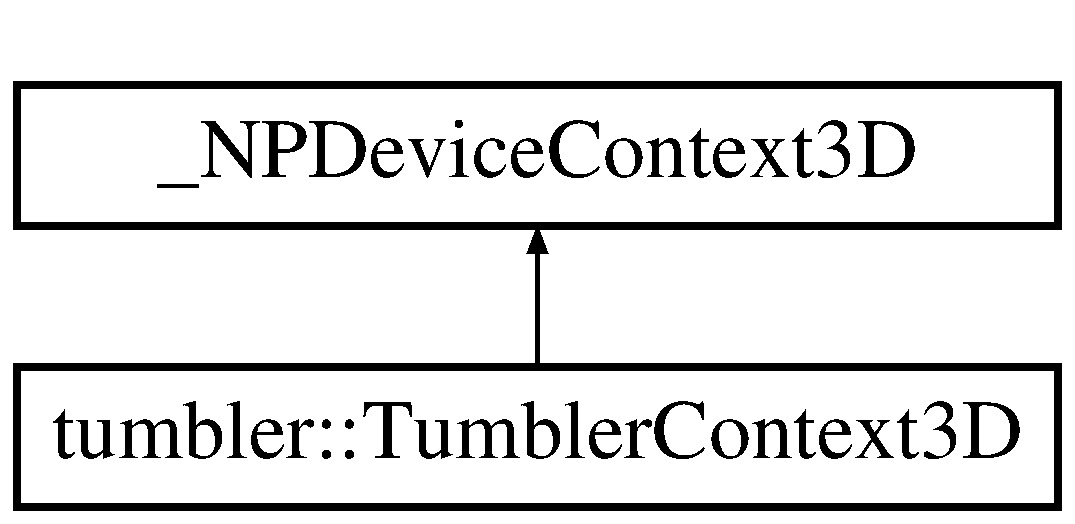
\includegraphics[height=2cm]{struct___n_p_device_context3_d}
\end{center}
\end{figure}
\subsection*{Public Attributes}
\begin{DoxyCompactItemize}
\item 
void $\ast$ \hyperlink{struct___n_p_device_context3_d_a98ffca8489323d94761d36927edbdc3c}{reserved}
\item 
bool \hyperlink{struct___n_p_device_context3_d_a652fa21fe68686fa83e81530d53e113e}{waitForProgress}
\item 
void $\ast$ \hyperlink{struct___n_p_device_context3_d_a92feeedd3fa2e4f14a9a0883e0883869}{commandBuffer}
\item 
int32\_\-t \hyperlink{struct___n_p_device_context3_d_af3d1a17e3a16355d530a2960d5167c7d}{commandBufferSize}
\item 
int32\_\-t \hyperlink{struct___n_p_device_context3_d_a94db0e726b7e3e3a421816ac896a8a51}{getOffset}
\item 
int32\_\-t \hyperlink{struct___n_p_device_context3_d_a95a001a05b4eb06f052a747f5521d2df}{putOffset}
\item 
int32\_\-t \hyperlink{struct___n_p_device_context3_d_a830ebfce87462205435ee2330f95b587}{token}
\item 
\hyperlink{npapi__extensions_8h_a619585c201cffd2cf885f5962c18acad}{NPDeviceContext3DRepaintPtr} \hyperlink{struct___n_p_device_context3_d_af5ba5d8f7cf171c710986a37dce757c8}{repaintCallback}
\item 
\hyperlink{npapi__extensions_8h_a906aa19cdf5fda7001f724a41118229a}{NPDeviceContext3DError} \hyperlink{struct___n_p_device_context3_d_a441e48d904459693f94a49f56ac9e419}{error}
\end{DoxyCompactItemize}


\subsection{Detailed Description}


Definition at line 759 of file npapi\_\-extensions.h.



\subsection{Member Data Documentation}
\hypertarget{struct___n_p_device_context3_d_a92feeedd3fa2e4f14a9a0883e0883869}{
\index{\_\-NPDeviceContext3D@{\_\-NPDeviceContext3D}!commandBuffer@{commandBuffer}}
\index{commandBuffer@{commandBuffer}!_NPDeviceContext3D@{\_\-NPDeviceContext3D}}
\subsubsection[{commandBuffer}]{\setlength{\rightskip}{0pt plus 5cm}void$\ast$ {\bf \_\-NPDeviceContext3D::commandBuffer}}}
\label{struct___n_p_device_context3_d_a92feeedd3fa2e4f14a9a0883e0883869}


Definition at line 774 of file npapi\_\-extensions.h.

\hypertarget{struct___n_p_device_context3_d_af3d1a17e3a16355d530a2960d5167c7d}{
\index{\_\-NPDeviceContext3D@{\_\-NPDeviceContext3D}!commandBufferSize@{commandBufferSize}}
\index{commandBufferSize@{commandBufferSize}!_NPDeviceContext3D@{\_\-NPDeviceContext3D}}
\subsubsection[{commandBufferSize}]{\setlength{\rightskip}{0pt plus 5cm}int32\_\-t {\bf \_\-NPDeviceContext3D::commandBufferSize}}}
\label{struct___n_p_device_context3_d_af3d1a17e3a16355d530a2960d5167c7d}


Definition at line 775 of file npapi\_\-extensions.h.

\hypertarget{struct___n_p_device_context3_d_a441e48d904459693f94a49f56ac9e419}{
\index{\_\-NPDeviceContext3D@{\_\-NPDeviceContext3D}!error@{error}}
\index{error@{error}!_NPDeviceContext3D@{\_\-NPDeviceContext3D}}
\subsubsection[{error}]{\setlength{\rightskip}{0pt plus 5cm}{\bf NPDeviceContext3DError} {\bf \_\-NPDeviceContext3D::error}}}
\label{struct___n_p_device_context3_d_a441e48d904459693f94a49f56ac9e419}


Definition at line 792 of file npapi\_\-extensions.h.

\hypertarget{struct___n_p_device_context3_d_a94db0e726b7e3e3a421816ac896a8a51}{
\index{\_\-NPDeviceContext3D@{\_\-NPDeviceContext3D}!getOffset@{getOffset}}
\index{getOffset@{getOffset}!_NPDeviceContext3D@{\_\-NPDeviceContext3D}}
\subsubsection[{getOffset}]{\setlength{\rightskip}{0pt plus 5cm}int32\_\-t {\bf \_\-NPDeviceContext3D::getOffset}}}
\label{struct___n_p_device_context3_d_a94db0e726b7e3e3a421816ac896a8a51}


Definition at line 778 of file npapi\_\-extensions.h.

\hypertarget{struct___n_p_device_context3_d_a95a001a05b4eb06f052a747f5521d2df}{
\index{\_\-NPDeviceContext3D@{\_\-NPDeviceContext3D}!putOffset@{putOffset}}
\index{putOffset@{putOffset}!_NPDeviceContext3D@{\_\-NPDeviceContext3D}}
\subsubsection[{putOffset}]{\setlength{\rightskip}{0pt plus 5cm}int32\_\-t {\bf \_\-NPDeviceContext3D::putOffset}}}
\label{struct___n_p_device_context3_d_a95a001a05b4eb06f052a747f5521d2df}


Definition at line 781 of file npapi\_\-extensions.h.

\hypertarget{struct___n_p_device_context3_d_af5ba5d8f7cf171c710986a37dce757c8}{
\index{\_\-NPDeviceContext3D@{\_\-NPDeviceContext3D}!repaintCallback@{repaintCallback}}
\index{repaintCallback@{repaintCallback}!_NPDeviceContext3D@{\_\-NPDeviceContext3D}}
\subsubsection[{repaintCallback}]{\setlength{\rightskip}{0pt plus 5cm}{\bf NPDeviceContext3DRepaintPtr} {\bf \_\-NPDeviceContext3D::repaintCallback}}}
\label{struct___n_p_device_context3_d_af5ba5d8f7cf171c710986a37dce757c8}


Definition at line 789 of file npapi\_\-extensions.h.

\hypertarget{struct___n_p_device_context3_d_a98ffca8489323d94761d36927edbdc3c}{
\index{\_\-NPDeviceContext3D@{\_\-NPDeviceContext3D}!reserved@{reserved}}
\index{reserved@{reserved}!_NPDeviceContext3D@{\_\-NPDeviceContext3D}}
\subsubsection[{reserved}]{\setlength{\rightskip}{0pt plus 5cm}void$\ast$ {\bf \_\-NPDeviceContext3D::reserved}}}
\label{struct___n_p_device_context3_d_a98ffca8489323d94761d36927edbdc3c}


Definition at line 761 of file npapi\_\-extensions.h.

\hypertarget{struct___n_p_device_context3_d_a830ebfce87462205435ee2330f95b587}{
\index{\_\-NPDeviceContext3D@{\_\-NPDeviceContext3D}!token@{token}}
\index{token@{token}!_NPDeviceContext3D@{\_\-NPDeviceContext3D}}
\subsubsection[{token}]{\setlength{\rightskip}{0pt plus 5cm}int32\_\-t {\bf \_\-NPDeviceContext3D::token}}}
\label{struct___n_p_device_context3_d_a830ebfce87462205435ee2330f95b587}


Definition at line 784 of file npapi\_\-extensions.h.

\hypertarget{struct___n_p_device_context3_d_a652fa21fe68686fa83e81530d53e113e}{
\index{\_\-NPDeviceContext3D@{\_\-NPDeviceContext3D}!waitForProgress@{waitForProgress}}
\index{waitForProgress@{waitForProgress}!_NPDeviceContext3D@{\_\-NPDeviceContext3D}}
\subsubsection[{waitForProgress}]{\setlength{\rightskip}{0pt plus 5cm}bool {\bf \_\-NPDeviceContext3D::waitForProgress}}}
\label{struct___n_p_device_context3_d_a652fa21fe68686fa83e81530d53e113e}


Definition at line 771 of file npapi\_\-extensions.h.



The documentation for this struct was generated from the following file:\begin{DoxyCompactItemize}
\item 
/home/derek/dev/cell-\/grid-\/game/nacl/crml/crml/core/\hyperlink{npapi__extensions_8h}{npapi\_\-extensions.h}\end{DoxyCompactItemize}

\hypertarget{struct___n_p_device_context3_d_config}{
\section{\_\-NPDeviceContext3DConfig Struct Reference}
\label{struct___n_p_device_context3_d_config}\index{\_\-NPDeviceContext3DConfig@{\_\-NPDeviceContext3DConfig}}
}


{\ttfamily \#include $<$npapi\_\-extensions.h$>$}

\subsection*{Public Attributes}
\begin{DoxyCompactItemize}
\item 
int32\_\-t \hyperlink{struct___n_p_device_context3_d_config_a0075edbd3e0c70d8db09dc0270c9bc76}{commandBufferSize}
\end{DoxyCompactItemize}


\subsection{Detailed Description}


Definition at line 724 of file npapi\_\-extensions.h.



\subsection{Member Data Documentation}
\hypertarget{struct___n_p_device_context3_d_config_a0075edbd3e0c70d8db09dc0270c9bc76}{
\index{\_\-NPDeviceContext3DConfig@{\_\-NPDeviceContext3DConfig}!commandBufferSize@{commandBufferSize}}
\index{commandBufferSize@{commandBufferSize}!_NPDeviceContext3DConfig@{\_\-NPDeviceContext3DConfig}}
\subsubsection[{commandBufferSize}]{\setlength{\rightskip}{0pt plus 5cm}int32\_\-t {\bf \_\-NPDeviceContext3DConfig::commandBufferSize}}}
\label{struct___n_p_device_context3_d_config_a0075edbd3e0c70d8db09dc0270c9bc76}


Definition at line 725 of file npapi\_\-extensions.h.



The documentation for this struct was generated from the following file:\begin{DoxyCompactItemize}
\item 
/home/derek/dev/cell-\/grid-\/game/nacl/crml/crml/core/\hyperlink{npapi__extensions_8h}{npapi\_\-extensions.h}\end{DoxyCompactItemize}

\hypertarget{struct___n_p_device_context_audio}{
\section{\_\-NPDeviceContextAudio Struct Reference}
\label{struct___n_p_device_context_audio}\index{\_\-NPDeviceContextAudio@{\_\-NPDeviceContextAudio}}
}


{\ttfamily \#include $<$npapi\_\-extensions.h$>$}

\subsection*{Public Attributes}
\begin{DoxyCompactItemize}
\item 
\hyperlink{struct___n_p_device_context_audio_config}{NPDeviceContextAudioConfig} \hyperlink{struct___n_p_device_context_audio_a77a64d9efc16465139b00f0939cebb71}{config}
\item 
void $\ast$ \hyperlink{struct___n_p_device_context_audio_a059607d2ba7cc02d5cdc10fc7e4b2b89}{outBuffer}
\item 
void $\ast$ \hyperlink{struct___n_p_device_context_audio_a8366d3cc305d9c97076ae202fa7eb4f3}{inBuffer}
\item 
void $\ast$ \hyperlink{struct___n_p_device_context_audio_a125bbc1c103ad897b7f2479d6ac34b6b}{reserved}
\end{DoxyCompactItemize}


\subsection{Detailed Description}


Definition at line 944 of file npapi\_\-extensions.h.



\subsection{Member Data Documentation}
\hypertarget{struct___n_p_device_context_audio_a77a64d9efc16465139b00f0939cebb71}{
\index{\_\-NPDeviceContextAudio@{\_\-NPDeviceContextAudio}!config@{config}}
\index{config@{config}!_NPDeviceContextAudio@{\_\-NPDeviceContextAudio}}
\subsubsection[{config}]{\setlength{\rightskip}{0pt plus 5cm}{\bf NPDeviceContextAudioConfig} {\bf \_\-NPDeviceContextAudio::config}}}
\label{struct___n_p_device_context_audio_a77a64d9efc16465139b00f0939cebb71}


Definition at line 945 of file npapi\_\-extensions.h.

\hypertarget{struct___n_p_device_context_audio_a8366d3cc305d9c97076ae202fa7eb4f3}{
\index{\_\-NPDeviceContextAudio@{\_\-NPDeviceContextAudio}!inBuffer@{inBuffer}}
\index{inBuffer@{inBuffer}!_NPDeviceContextAudio@{\_\-NPDeviceContextAudio}}
\subsubsection[{inBuffer}]{\setlength{\rightskip}{0pt plus 5cm}void$\ast$ {\bf \_\-NPDeviceContextAudio::inBuffer}}}
\label{struct___n_p_device_context_audio_a8366d3cc305d9c97076ae202fa7eb4f3}


Definition at line 947 of file npapi\_\-extensions.h.

\hypertarget{struct___n_p_device_context_audio_a059607d2ba7cc02d5cdc10fc7e4b2b89}{
\index{\_\-NPDeviceContextAudio@{\_\-NPDeviceContextAudio}!outBuffer@{outBuffer}}
\index{outBuffer@{outBuffer}!_NPDeviceContextAudio@{\_\-NPDeviceContextAudio}}
\subsubsection[{outBuffer}]{\setlength{\rightskip}{0pt plus 5cm}void$\ast$ {\bf \_\-NPDeviceContextAudio::outBuffer}}}
\label{struct___n_p_device_context_audio_a059607d2ba7cc02d5cdc10fc7e4b2b89}


Definition at line 946 of file npapi\_\-extensions.h.

\hypertarget{struct___n_p_device_context_audio_a125bbc1c103ad897b7f2479d6ac34b6b}{
\index{\_\-NPDeviceContextAudio@{\_\-NPDeviceContextAudio}!reserved@{reserved}}
\index{reserved@{reserved}!_NPDeviceContextAudio@{\_\-NPDeviceContextAudio}}
\subsubsection[{reserved}]{\setlength{\rightskip}{0pt plus 5cm}void$\ast$ {\bf \_\-NPDeviceContextAudio::reserved}}}
\label{struct___n_p_device_context_audio_a125bbc1c103ad897b7f2479d6ac34b6b}


Definition at line 948 of file npapi\_\-extensions.h.



The documentation for this struct was generated from the following file:\begin{DoxyCompactItemize}
\item 
/home/derek/dev/cell-\/grid-\/game/nacl/crml/crml/core/\hyperlink{npapi__extensions_8h}{npapi\_\-extensions.h}\end{DoxyCompactItemize}

\hypertarget{struct___n_p_device_context_audio_config}{
\section{\_\-NPDeviceContextAudioConfig Struct Reference}
\label{struct___n_p_device_context_audio_config}\index{\_\-NPDeviceContextAudioConfig@{\_\-NPDeviceContextAudioConfig}}
}


{\ttfamily \#include $<$npapi\_\-extensions.h$>$}

\subsection*{Public Attributes}
\begin{DoxyCompactItemize}
\item 
int32\_\-t \hyperlink{struct___n_p_device_context_audio_config_ae8f165b45aa2bb33a84d4e62c320afef}{sampleRate}
\item 
int32\_\-t \hyperlink{struct___n_p_device_context_audio_config_a72368bc2db5c560fcfcec9f048fe7e93}{sampleType}
\item 
int32\_\-t \hyperlink{struct___n_p_device_context_audio_config_adc7b8d1ae23a27b833dd9816ca76c9b2}{outputChannelMap}
\item 
int32\_\-t \hyperlink{struct___n_p_device_context_audio_config_a69c0328c3256924a80490c75b643cfd9}{inputChannelMap}
\item 
int32\_\-t \hyperlink{struct___n_p_device_context_audio_config_a9845d796ed525af2eef523a8246d5fff}{sampleFrameCount}
\item 
uint32\_\-t \hyperlink{struct___n_p_device_context_audio_config_a4456ec356a3d5da2b9d05d8de19868ee}{startThread}
\item 
uint32\_\-t \hyperlink{struct___n_p_device_context_audio_config_a50ce2ce4d00b584205cdfe725d43c760}{flags}
\item 
\hyperlink{npapi__extensions_8h_ac16a100eeec4f1d8a44e1d4e4a55cd31}{NPAudioCallback} \hyperlink{struct___n_p_device_context_audio_config_a913925b7c8aceb040e26433e9b68b577}{callback}
\item 
void $\ast$ \hyperlink{struct___n_p_device_context_audio_config_a02dc164c09c13d1a97adde1544a0a787}{userData}
\end{DoxyCompactItemize}


\subsection{Detailed Description}


Definition at line 932 of file npapi\_\-extensions.h.



\subsection{Member Data Documentation}
\hypertarget{struct___n_p_device_context_audio_config_a913925b7c8aceb040e26433e9b68b577}{
\index{\_\-NPDeviceContextAudioConfig@{\_\-NPDeviceContextAudioConfig}!callback@{callback}}
\index{callback@{callback}!_NPDeviceContextAudioConfig@{\_\-NPDeviceContextAudioConfig}}
\subsubsection[{callback}]{\setlength{\rightskip}{0pt plus 5cm}{\bf NPAudioCallback} {\bf \_\-NPDeviceContextAudioConfig::callback}}}
\label{struct___n_p_device_context_audio_config_a913925b7c8aceb040e26433e9b68b577}


Definition at line 940 of file npapi\_\-extensions.h.

\hypertarget{struct___n_p_device_context_audio_config_a50ce2ce4d00b584205cdfe725d43c760}{
\index{\_\-NPDeviceContextAudioConfig@{\_\-NPDeviceContextAudioConfig}!flags@{flags}}
\index{flags@{flags}!_NPDeviceContextAudioConfig@{\_\-NPDeviceContextAudioConfig}}
\subsubsection[{flags}]{\setlength{\rightskip}{0pt plus 5cm}uint32\_\-t {\bf \_\-NPDeviceContextAudioConfig::flags}}}
\label{struct___n_p_device_context_audio_config_a50ce2ce4d00b584205cdfe725d43c760}


Definition at line 939 of file npapi\_\-extensions.h.

\hypertarget{struct___n_p_device_context_audio_config_a69c0328c3256924a80490c75b643cfd9}{
\index{\_\-NPDeviceContextAudioConfig@{\_\-NPDeviceContextAudioConfig}!inputChannelMap@{inputChannelMap}}
\index{inputChannelMap@{inputChannelMap}!_NPDeviceContextAudioConfig@{\_\-NPDeviceContextAudioConfig}}
\subsubsection[{inputChannelMap}]{\setlength{\rightskip}{0pt plus 5cm}int32\_\-t {\bf \_\-NPDeviceContextAudioConfig::inputChannelMap}}}
\label{struct___n_p_device_context_audio_config_a69c0328c3256924a80490c75b643cfd9}


Definition at line 936 of file npapi\_\-extensions.h.

\hypertarget{struct___n_p_device_context_audio_config_adc7b8d1ae23a27b833dd9816ca76c9b2}{
\index{\_\-NPDeviceContextAudioConfig@{\_\-NPDeviceContextAudioConfig}!outputChannelMap@{outputChannelMap}}
\index{outputChannelMap@{outputChannelMap}!_NPDeviceContextAudioConfig@{\_\-NPDeviceContextAudioConfig}}
\subsubsection[{outputChannelMap}]{\setlength{\rightskip}{0pt plus 5cm}int32\_\-t {\bf \_\-NPDeviceContextAudioConfig::outputChannelMap}}}
\label{struct___n_p_device_context_audio_config_adc7b8d1ae23a27b833dd9816ca76c9b2}


Definition at line 935 of file npapi\_\-extensions.h.

\hypertarget{struct___n_p_device_context_audio_config_a9845d796ed525af2eef523a8246d5fff}{
\index{\_\-NPDeviceContextAudioConfig@{\_\-NPDeviceContextAudioConfig}!sampleFrameCount@{sampleFrameCount}}
\index{sampleFrameCount@{sampleFrameCount}!_NPDeviceContextAudioConfig@{\_\-NPDeviceContextAudioConfig}}
\subsubsection[{sampleFrameCount}]{\setlength{\rightskip}{0pt plus 5cm}int32\_\-t {\bf \_\-NPDeviceContextAudioConfig::sampleFrameCount}}}
\label{struct___n_p_device_context_audio_config_a9845d796ed525af2eef523a8246d5fff}


Definition at line 937 of file npapi\_\-extensions.h.

\hypertarget{struct___n_p_device_context_audio_config_ae8f165b45aa2bb33a84d4e62c320afef}{
\index{\_\-NPDeviceContextAudioConfig@{\_\-NPDeviceContextAudioConfig}!sampleRate@{sampleRate}}
\index{sampleRate@{sampleRate}!_NPDeviceContextAudioConfig@{\_\-NPDeviceContextAudioConfig}}
\subsubsection[{sampleRate}]{\setlength{\rightskip}{0pt plus 5cm}int32\_\-t {\bf \_\-NPDeviceContextAudioConfig::sampleRate}}}
\label{struct___n_p_device_context_audio_config_ae8f165b45aa2bb33a84d4e62c320afef}


Definition at line 933 of file npapi\_\-extensions.h.

\hypertarget{struct___n_p_device_context_audio_config_a72368bc2db5c560fcfcec9f048fe7e93}{
\index{\_\-NPDeviceContextAudioConfig@{\_\-NPDeviceContextAudioConfig}!sampleType@{sampleType}}
\index{sampleType@{sampleType}!_NPDeviceContextAudioConfig@{\_\-NPDeviceContextAudioConfig}}
\subsubsection[{sampleType}]{\setlength{\rightskip}{0pt plus 5cm}int32\_\-t {\bf \_\-NPDeviceContextAudioConfig::sampleType}}}
\label{struct___n_p_device_context_audio_config_a72368bc2db5c560fcfcec9f048fe7e93}


Definition at line 934 of file npapi\_\-extensions.h.

\hypertarget{struct___n_p_device_context_audio_config_a4456ec356a3d5da2b9d05d8de19868ee}{
\index{\_\-NPDeviceContextAudioConfig@{\_\-NPDeviceContextAudioConfig}!startThread@{startThread}}
\index{startThread@{startThread}!_NPDeviceContextAudioConfig@{\_\-NPDeviceContextAudioConfig}}
\subsubsection[{startThread}]{\setlength{\rightskip}{0pt plus 5cm}uint32\_\-t {\bf \_\-NPDeviceContextAudioConfig::startThread}}}
\label{struct___n_p_device_context_audio_config_a4456ec356a3d5da2b9d05d8de19868ee}


Definition at line 938 of file npapi\_\-extensions.h.

\hypertarget{struct___n_p_device_context_audio_config_a02dc164c09c13d1a97adde1544a0a787}{
\index{\_\-NPDeviceContextAudioConfig@{\_\-NPDeviceContextAudioConfig}!userData@{userData}}
\index{userData@{userData}!_NPDeviceContextAudioConfig@{\_\-NPDeviceContextAudioConfig}}
\subsubsection[{userData}]{\setlength{\rightskip}{0pt plus 5cm}void$\ast$ {\bf \_\-NPDeviceContextAudioConfig::userData}}}
\label{struct___n_p_device_context_audio_config_a02dc164c09c13d1a97adde1544a0a787}


Definition at line 941 of file npapi\_\-extensions.h.



The documentation for this struct was generated from the following file:\begin{DoxyCompactItemize}
\item 
/home/derek/dev/cell-\/grid-\/game/nacl/crml/crml/core/\hyperlink{npapi__extensions_8h}{npapi\_\-extensions.h}\end{DoxyCompactItemize}

\hypertarget{struct___n_p_device_event}{
\section{\_\-NPDeviceEvent Struct Reference}
\label{struct___n_p_device_event}\index{\_\-NPDeviceEvent@{\_\-NPDeviceEvent}}
}


{\ttfamily \#include $<$npapi\_\-extensions.h$>$}

\subsection*{Public Attributes}
\begin{DoxyCompactItemize}
\item 
uint32\_\-t \hyperlink{struct___n_p_device_event_a3fdf3b1d49f5717880ebb0714f865271}{device\_\-uid}
\item 
uint32\_\-t \hyperlink{struct___n_p_device_event_ad8659828b3af02ef9e65dbc9fac6b069}{subtype}
\end{DoxyCompactItemize}


\subsection{Detailed Description}


Definition at line 100 of file npapi\_\-extensions.h.



\subsection{Member Data Documentation}
\hypertarget{struct___n_p_device_event_a3fdf3b1d49f5717880ebb0714f865271}{
\index{\_\-NPDeviceEvent@{\_\-NPDeviceEvent}!device\_\-uid@{device\_\-uid}}
\index{device\_\-uid@{device\_\-uid}!_NPDeviceEvent@{\_\-NPDeviceEvent}}
\subsubsection[{device\_\-uid}]{\setlength{\rightskip}{0pt plus 5cm}uint32\_\-t {\bf \_\-NPDeviceEvent::device\_\-uid}}}
\label{struct___n_p_device_event_a3fdf3b1d49f5717880ebb0714f865271}


Definition at line 101 of file npapi\_\-extensions.h.

\hypertarget{struct___n_p_device_event_ad8659828b3af02ef9e65dbc9fac6b069}{
\index{\_\-NPDeviceEvent@{\_\-NPDeviceEvent}!subtype@{subtype}}
\index{subtype@{subtype}!_NPDeviceEvent@{\_\-NPDeviceEvent}}
\subsubsection[{subtype}]{\setlength{\rightskip}{0pt plus 5cm}uint32\_\-t {\bf \_\-NPDeviceEvent::subtype}}}
\label{struct___n_p_device_event_ad8659828b3af02ef9e65dbc9fac6b069}


Definition at line 102 of file npapi\_\-extensions.h.



The documentation for this struct was generated from the following file:\begin{DoxyCompactItemize}
\item 
/home/derek/dev/cell-\/grid-\/game/nacl/crml/crml/core/\hyperlink{npapi__extensions_8h}{npapi\_\-extensions.h}\end{DoxyCompactItemize}

\hypertarget{struct___n_p_embed_print}{
\section{\_\-NPEmbedPrint Struct Reference}
\label{struct___n_p_embed_print}\index{\_\-NPEmbedPrint@{\_\-NPEmbedPrint}}
}


{\ttfamily \#include $<$npapi.h$>$}

\subsection*{Public Attributes}
\begin{DoxyCompactItemize}
\item 
\hyperlink{struct___n_p_window}{NPWindow} \hyperlink{struct___n_p_embed_print_a875099b1a13499d56ae6c84ade550a94}{window}
\item 
void $\ast$ \hyperlink{struct___n_p_embed_print_a147fecd7cac88b8873814bc493241b6e}{platformPrint}
\end{DoxyCompactItemize}


\subsection{Detailed Description}


Definition at line 505 of file npapi.h.



\subsection{Member Data Documentation}
\hypertarget{struct___n_p_embed_print_a147fecd7cac88b8873814bc493241b6e}{
\index{\_\-NPEmbedPrint@{\_\-NPEmbedPrint}!platformPrint@{platformPrint}}
\index{platformPrint@{platformPrint}!_NPEmbedPrint@{\_\-NPEmbedPrint}}
\subsubsection[{platformPrint}]{\setlength{\rightskip}{0pt plus 5cm}void$\ast$ {\bf \_\-NPEmbedPrint::platformPrint}}}
\label{struct___n_p_embed_print_a147fecd7cac88b8873814bc493241b6e}


Definition at line 508 of file npapi.h.

\hypertarget{struct___n_p_embed_print_a875099b1a13499d56ae6c84ade550a94}{
\index{\_\-NPEmbedPrint@{\_\-NPEmbedPrint}!window@{window}}
\index{window@{window}!_NPEmbedPrint@{\_\-NPEmbedPrint}}
\subsubsection[{window}]{\setlength{\rightskip}{0pt plus 5cm}{\bf NPWindow} {\bf \_\-NPEmbedPrint::window}}}
\label{struct___n_p_embed_print_a875099b1a13499d56ae6c84ade550a94}


Definition at line 507 of file npapi.h.



The documentation for this struct was generated from the following file:\begin{DoxyCompactItemize}
\item 
/home/derek/dev/cell-\/grid-\/game/nacl/crml/crml/core/\hyperlink{npapi_8h}{npapi.h}\end{DoxyCompactItemize}

\hypertarget{struct___n_p_focus_event}{
\section{\_\-NPFocusEvent Struct Reference}
\label{struct___n_p_focus_event}\index{\_\-NPFocusEvent@{\_\-NPFocusEvent}}
}


{\ttfamily \#include $<$npapi\_\-extensions.h$>$}

\subsection*{Public Attributes}
\begin{DoxyCompactItemize}
\item 
int32\_\-t \hyperlink{struct___n_p_focus_event_af4f66adf55aa4501d2a8b67dbc421210}{value}
\end{DoxyCompactItemize}


\subsection{Detailed Description}


Definition at line 110 of file npapi\_\-extensions.h.



\subsection{Member Data Documentation}
\hypertarget{struct___n_p_focus_event_af4f66adf55aa4501d2a8b67dbc421210}{
\index{\_\-NPFocusEvent@{\_\-NPFocusEvent}!value@{value}}
\index{value@{value}!_NPFocusEvent@{\_\-NPFocusEvent}}
\subsubsection[{value}]{\setlength{\rightskip}{0pt plus 5cm}int32\_\-t {\bf \_\-NPFocusEvent::value}}}
\label{struct___n_p_focus_event_af4f66adf55aa4501d2a8b67dbc421210}


Definition at line 111 of file npapi\_\-extensions.h.



The documentation for this struct was generated from the following file:\begin{DoxyCompactItemize}
\item 
/home/derek/dev/cell-\/grid-\/game/nacl/crml/crml/core/\hyperlink{npapi__extensions_8h}{npapi\_\-extensions.h}\end{DoxyCompactItemize}

\hypertarget{struct___n_p_font_description}{
\section{\_\-NPFontDescription Struct Reference}
\label{struct___n_p_font_description}\index{\_\-NPFontDescription@{\_\-NPFontDescription}}
}


{\ttfamily \#include $<$npapi\_\-extensions.h$>$}

\subsection*{Public Attributes}
\begin{DoxyCompactItemize}
\item 
const char $\ast$ \hyperlink{struct___n_p_font_description_aeca685fa53dc898a3f38d55dc2cf3941}{face}
\item 
int \hyperlink{struct___n_p_font_description_ab23cb8515f8fb97a71c2114706284361}{weight}
\item 
bool \hyperlink{struct___n_p_font_description_aa0b5f70dec32b8a74627b7bc210219f5}{italic}
\item 
\hyperlink{npapi__extensions_8h_a3eae6a1f6a13d35171a4bd5f6c6b35a8}{NPPitch} \hyperlink{struct___n_p_font_description_a669fa154e09a6a682c727bf6bccc028b}{pitch}
\item 
\hyperlink{npapi__extensions_8h_a34cbc00a891faea17015ea04c0c30083}{NPFamily} \hyperlink{struct___n_p_font_description_ac78f86d50687284c1b20b3ea05f26501}{family}
\item 
\hyperlink{npapi__extensions_8h_a8d338781e5a4a188e3cb597be4e5bbe2}{NPCharset} \hyperlink{struct___n_p_font_description_a1e9e61b07f5df852ef3a5908cd35a242}{charset}
\end{DoxyCompactItemize}


\subsection{Detailed Description}


Definition at line 662 of file npapi\_\-extensions.h.



\subsection{Member Data Documentation}
\hypertarget{struct___n_p_font_description_a1e9e61b07f5df852ef3a5908cd35a242}{
\index{\_\-NPFontDescription@{\_\-NPFontDescription}!charset@{charset}}
\index{charset@{charset}!_NPFontDescription@{\_\-NPFontDescription}}
\subsubsection[{charset}]{\setlength{\rightskip}{0pt plus 5cm}{\bf NPCharset} {\bf \_\-NPFontDescription::charset}}}
\label{struct___n_p_font_description_a1e9e61b07f5df852ef3a5908cd35a242}


Definition at line 668 of file npapi\_\-extensions.h.

\hypertarget{struct___n_p_font_description_aeca685fa53dc898a3f38d55dc2cf3941}{
\index{\_\-NPFontDescription@{\_\-NPFontDescription}!face@{face}}
\index{face@{face}!_NPFontDescription@{\_\-NPFontDescription}}
\subsubsection[{face}]{\setlength{\rightskip}{0pt plus 5cm}const char$\ast$ {\bf \_\-NPFontDescription::face}}}
\label{struct___n_p_font_description_aeca685fa53dc898a3f38d55dc2cf3941}


Definition at line 663 of file npapi\_\-extensions.h.

\hypertarget{struct___n_p_font_description_ac78f86d50687284c1b20b3ea05f26501}{
\index{\_\-NPFontDescription@{\_\-NPFontDescription}!family@{family}}
\index{family@{family}!_NPFontDescription@{\_\-NPFontDescription}}
\subsubsection[{family}]{\setlength{\rightskip}{0pt plus 5cm}{\bf NPFamily} {\bf \_\-NPFontDescription::family}}}
\label{struct___n_p_font_description_ac78f86d50687284c1b20b3ea05f26501}


Definition at line 667 of file npapi\_\-extensions.h.

\hypertarget{struct___n_p_font_description_aa0b5f70dec32b8a74627b7bc210219f5}{
\index{\_\-NPFontDescription@{\_\-NPFontDescription}!italic@{italic}}
\index{italic@{italic}!_NPFontDescription@{\_\-NPFontDescription}}
\subsubsection[{italic}]{\setlength{\rightskip}{0pt plus 5cm}bool {\bf \_\-NPFontDescription::italic}}}
\label{struct___n_p_font_description_aa0b5f70dec32b8a74627b7bc210219f5}


Definition at line 665 of file npapi\_\-extensions.h.

\hypertarget{struct___n_p_font_description_a669fa154e09a6a682c727bf6bccc028b}{
\index{\_\-NPFontDescription@{\_\-NPFontDescription}!pitch@{pitch}}
\index{pitch@{pitch}!_NPFontDescription@{\_\-NPFontDescription}}
\subsubsection[{pitch}]{\setlength{\rightskip}{0pt plus 5cm}{\bf NPPitch} {\bf \_\-NPFontDescription::pitch}}}
\label{struct___n_p_font_description_a669fa154e09a6a682c727bf6bccc028b}


Definition at line 666 of file npapi\_\-extensions.h.

\hypertarget{struct___n_p_font_description_ab23cb8515f8fb97a71c2114706284361}{
\index{\_\-NPFontDescription@{\_\-NPFontDescription}!weight@{weight}}
\index{weight@{weight}!_NPFontDescription@{\_\-NPFontDescription}}
\subsubsection[{weight}]{\setlength{\rightskip}{0pt plus 5cm}int {\bf \_\-NPFontDescription::weight}}}
\label{struct___n_p_font_description_ab23cb8515f8fb97a71c2114706284361}


Definition at line 664 of file npapi\_\-extensions.h.



The documentation for this struct was generated from the following file:\begin{DoxyCompactItemize}
\item 
/home/derek/dev/cell-\/grid-\/game/nacl/crml/crml/core/\hyperlink{npapi__extensions_8h}{npapi\_\-extensions.h}\end{DoxyCompactItemize}

\hypertarget{struct___n_p_font_extensions}{
\section{\_\-NPFontExtensions Struct Reference}
\label{struct___n_p_font_extensions}\index{\_\-NPFontExtensions@{\_\-NPFontExtensions}}
}


{\ttfamily \#include $<$npapi\_\-extensions.h$>$}

\subsection*{Public Attributes}
\begin{DoxyCompactItemize}
\item 
\hyperlink{npapi__extensions_8h_a34e4527ad657576de1f6ade509b9bdf0}{NPMatchFontWithFallbackPtr} \hyperlink{struct___n_p_font_extensions_a76de211ff3a72e2ece70f6c54d81a816}{matchFontWithFallback}
\item 
\hyperlink{npapi__extensions_8h_aa4528a94d7c4edaf308a784b25310069}{GetFontTablePtr} \hyperlink{struct___n_p_font_extensions_a7e7d1715bdf84093be3e08f98a986b2b}{getFontTable}
\item 
\hyperlink{npapi__extensions_8h_a18516feaf8eb67200682c7b55f0844a5}{NPDestroyFontPtr} \hyperlink{struct___n_p_font_extensions_a1e3bbc4b7ee955799f9805e8a0ccc3dc}{destroyFont}
\end{DoxyCompactItemize}


\subsection{Detailed Description}


Definition at line 694 of file npapi\_\-extensions.h.



\subsection{Member Data Documentation}
\hypertarget{struct___n_p_font_extensions_a1e3bbc4b7ee955799f9805e8a0ccc3dc}{
\index{\_\-NPFontExtensions@{\_\-NPFontExtensions}!destroyFont@{destroyFont}}
\index{destroyFont@{destroyFont}!_NPFontExtensions@{\_\-NPFontExtensions}}
\subsubsection[{destroyFont}]{\setlength{\rightskip}{0pt plus 5cm}{\bf NPDestroyFontPtr} {\bf \_\-NPFontExtensions::destroyFont}}}
\label{struct___n_p_font_extensions_a1e3bbc4b7ee955799f9805e8a0ccc3dc}


Definition at line 697 of file npapi\_\-extensions.h.

\hypertarget{struct___n_p_font_extensions_a7e7d1715bdf84093be3e08f98a986b2b}{
\index{\_\-NPFontExtensions@{\_\-NPFontExtensions}!getFontTable@{getFontTable}}
\index{getFontTable@{getFontTable}!_NPFontExtensions@{\_\-NPFontExtensions}}
\subsubsection[{getFontTable}]{\setlength{\rightskip}{0pt plus 5cm}{\bf GetFontTablePtr} {\bf \_\-NPFontExtensions::getFontTable}}}
\label{struct___n_p_font_extensions_a7e7d1715bdf84093be3e08f98a986b2b}


Definition at line 696 of file npapi\_\-extensions.h.

\hypertarget{struct___n_p_font_extensions_a76de211ff3a72e2ece70f6c54d81a816}{
\index{\_\-NPFontExtensions@{\_\-NPFontExtensions}!matchFontWithFallback@{matchFontWithFallback}}
\index{matchFontWithFallback@{matchFontWithFallback}!_NPFontExtensions@{\_\-NPFontExtensions}}
\subsubsection[{matchFontWithFallback}]{\setlength{\rightskip}{0pt plus 5cm}{\bf NPMatchFontWithFallbackPtr} {\bf \_\-NPFontExtensions::matchFontWithFallback}}}
\label{struct___n_p_font_extensions_a76de211ff3a72e2ece70f6c54d81a816}


Definition at line 695 of file npapi\_\-extensions.h.



The documentation for this struct was generated from the following file:\begin{DoxyCompactItemize}
\item 
/home/derek/dev/cell-\/grid-\/game/nacl/crml/crml/core/\hyperlink{npapi__extensions_8h}{npapi\_\-extensions.h}\end{DoxyCompactItemize}

\hypertarget{struct___n_p_full_print}{
\section{\_\-NPFullPrint Struct Reference}
\label{struct___n_p_full_print}\index{\_\-NPFullPrint@{\_\-NPFullPrint}}
}


{\ttfamily \#include $<$npapi.h$>$}

\subsection*{Public Attributes}
\begin{DoxyCompactItemize}
\item 
\hyperlink{npapi_8h_acaaa85dcdc33ec2865fb0544f1792142}{NPBool} \hyperlink{struct___n_p_full_print_a3ca77a50210f8e9e8232992b3ab7682e}{pluginPrinted}
\item 
\hyperlink{npapi_8h_acaaa85dcdc33ec2865fb0544f1792142}{NPBool} \hyperlink{struct___n_p_full_print_a809c29777645db1a739e48a30803c1f1}{printOne}
\item 
void $\ast$ \hyperlink{struct___n_p_full_print_a747b4c22896b774a1746715dce29c609}{platformPrint}
\end{DoxyCompactItemize}


\subsection{Detailed Description}


Definition at line 497 of file npapi.h.



\subsection{Member Data Documentation}
\hypertarget{struct___n_p_full_print_a747b4c22896b774a1746715dce29c609}{
\index{\_\-NPFullPrint@{\_\-NPFullPrint}!platformPrint@{platformPrint}}
\index{platformPrint@{platformPrint}!_NPFullPrint@{\_\-NPFullPrint}}
\subsubsection[{platformPrint}]{\setlength{\rightskip}{0pt plus 5cm}void$\ast$ {\bf \_\-NPFullPrint::platformPrint}}}
\label{struct___n_p_full_print_a747b4c22896b774a1746715dce29c609}


Definition at line 502 of file npapi.h.

\hypertarget{struct___n_p_full_print_a3ca77a50210f8e9e8232992b3ab7682e}{
\index{\_\-NPFullPrint@{\_\-NPFullPrint}!pluginPrinted@{pluginPrinted}}
\index{pluginPrinted@{pluginPrinted}!_NPFullPrint@{\_\-NPFullPrint}}
\subsubsection[{pluginPrinted}]{\setlength{\rightskip}{0pt plus 5cm}{\bf NPBool} {\bf \_\-NPFullPrint::pluginPrinted}}}
\label{struct___n_p_full_print_a3ca77a50210f8e9e8232992b3ab7682e}


Definition at line 499 of file npapi.h.

\hypertarget{struct___n_p_full_print_a809c29777645db1a739e48a30803c1f1}{
\index{\_\-NPFullPrint@{\_\-NPFullPrint}!printOne@{printOne}}
\index{printOne@{printOne}!_NPFullPrint@{\_\-NPFullPrint}}
\subsubsection[{printOne}]{\setlength{\rightskip}{0pt plus 5cm}{\bf NPBool} {\bf \_\-NPFullPrint::printOne}}}
\label{struct___n_p_full_print_a809c29777645db1a739e48a30803c1f1}


Definition at line 500 of file npapi.h.



The documentation for this struct was generated from the following file:\begin{DoxyCompactItemize}
\item 
/home/derek/dev/cell-\/grid-\/game/nacl/crml/crml/core/\hyperlink{npapi_8h}{npapi.h}\end{DoxyCompactItemize}

\hypertarget{struct___n_p_image_expose}{
\section{\_\-NPImageExpose Struct Reference}
\label{struct___n_p_image_expose}\index{\_\-NPImageExpose@{\_\-NPImageExpose}}
}


{\ttfamily \#include $<$npapi.h$>$}

\subsection*{Public Attributes}
\begin{DoxyCompactItemize}
\item 
char $\ast$ \hyperlink{struct___n_p_image_expose_a4261d6867119c1ffe0bd4fe44cbaa4d0}{data}
\item 
int32\_\-t \hyperlink{struct___n_p_image_expose_a615500c6ef3cea7b86f61a02bd8dfbcf}{stride}
\item 
int32\_\-t \hyperlink{struct___n_p_image_expose_aaef2311fadc6309c258e045087706697}{depth}
\item 
int32\_\-t \hyperlink{struct___n_p_image_expose_a636eff0e6eb37cc897f3968e2bbcd645}{x}
\item 
int32\_\-t \hyperlink{struct___n_p_image_expose_a25c47ac7da24f57ef6bba671e1b8d33b}{y}
\item 
uint32\_\-t \hyperlink{struct___n_p_image_expose_ac250a8831a9bc7b97ea911baa38a17b5}{width}
\item 
uint32\_\-t \hyperlink{struct___n_p_image_expose_a6f672c7697b1e6a029278bacacd7936a}{height}
\item 
\hyperlink{struct___n_p_size}{NPSize} \hyperlink{struct___n_p_image_expose_a38e94219212019a5e5f3fb87b6634e82}{dataSize}
\item 
float \hyperlink{struct___n_p_image_expose_a7ccc8c007a7033f1cf6620bf05d917c4}{translateX}
\item 
float \hyperlink{struct___n_p_image_expose_ab7a799a5a3cf7efeaca5eb0fc1d5265d}{translateY}
\item 
float \hyperlink{struct___n_p_image_expose_a459e533407f02b3b01de9307a26acf70}{scaleX}
\item 
float \hyperlink{struct___n_p_image_expose_a758b274482a925e928a9c452bf500ede}{scaleY}
\end{DoxyCompactItemize}


\subsection{Detailed Description}


Definition at line 481 of file npapi.h.



\subsection{Member Data Documentation}
\hypertarget{struct___n_p_image_expose_a4261d6867119c1ffe0bd4fe44cbaa4d0}{
\index{\_\-NPImageExpose@{\_\-NPImageExpose}!data@{data}}
\index{data@{data}!_NPImageExpose@{\_\-NPImageExpose}}
\subsubsection[{data}]{\setlength{\rightskip}{0pt plus 5cm}char$\ast$ {\bf \_\-NPImageExpose::data}}}
\label{struct___n_p_image_expose_a4261d6867119c1ffe0bd4fe44cbaa4d0}


Definition at line 483 of file npapi.h.

\hypertarget{struct___n_p_image_expose_a38e94219212019a5e5f3fb87b6634e82}{
\index{\_\-NPImageExpose@{\_\-NPImageExpose}!dataSize@{dataSize}}
\index{dataSize@{dataSize}!_NPImageExpose@{\_\-NPImageExpose}}
\subsubsection[{dataSize}]{\setlength{\rightskip}{0pt plus 5cm}{\bf NPSize} {\bf \_\-NPImageExpose::dataSize}}}
\label{struct___n_p_image_expose_a38e94219212019a5e5f3fb87b6634e82}


Definition at line 490 of file npapi.h.

\hypertarget{struct___n_p_image_expose_aaef2311fadc6309c258e045087706697}{
\index{\_\-NPImageExpose@{\_\-NPImageExpose}!depth@{depth}}
\index{depth@{depth}!_NPImageExpose@{\_\-NPImageExpose}}
\subsubsection[{depth}]{\setlength{\rightskip}{0pt plus 5cm}int32\_\-t {\bf \_\-NPImageExpose::depth}}}
\label{struct___n_p_image_expose_aaef2311fadc6309c258e045087706697}


Definition at line 485 of file npapi.h.

\hypertarget{struct___n_p_image_expose_a6f672c7697b1e6a029278bacacd7936a}{
\index{\_\-NPImageExpose@{\_\-NPImageExpose}!height@{height}}
\index{height@{height}!_NPImageExpose@{\_\-NPImageExpose}}
\subsubsection[{height}]{\setlength{\rightskip}{0pt plus 5cm}uint32\_\-t {\bf \_\-NPImageExpose::height}}}
\label{struct___n_p_image_expose_a6f672c7697b1e6a029278bacacd7936a}


Definition at line 489 of file npapi.h.

\hypertarget{struct___n_p_image_expose_a459e533407f02b3b01de9307a26acf70}{
\index{\_\-NPImageExpose@{\_\-NPImageExpose}!scaleX@{scaleX}}
\index{scaleX@{scaleX}!_NPImageExpose@{\_\-NPImageExpose}}
\subsubsection[{scaleX}]{\setlength{\rightskip}{0pt plus 5cm}float {\bf \_\-NPImageExpose::scaleX}}}
\label{struct___n_p_image_expose_a459e533407f02b3b01de9307a26acf70}


Definition at line 493 of file npapi.h.

\hypertarget{struct___n_p_image_expose_a758b274482a925e928a9c452bf500ede}{
\index{\_\-NPImageExpose@{\_\-NPImageExpose}!scaleY@{scaleY}}
\index{scaleY@{scaleY}!_NPImageExpose@{\_\-NPImageExpose}}
\subsubsection[{scaleY}]{\setlength{\rightskip}{0pt plus 5cm}float {\bf \_\-NPImageExpose::scaleY}}}
\label{struct___n_p_image_expose_a758b274482a925e928a9c452bf500ede}


Definition at line 494 of file npapi.h.

\hypertarget{struct___n_p_image_expose_a615500c6ef3cea7b86f61a02bd8dfbcf}{
\index{\_\-NPImageExpose@{\_\-NPImageExpose}!stride@{stride}}
\index{stride@{stride}!_NPImageExpose@{\_\-NPImageExpose}}
\subsubsection[{stride}]{\setlength{\rightskip}{0pt plus 5cm}int32\_\-t {\bf \_\-NPImageExpose::stride}}}
\label{struct___n_p_image_expose_a615500c6ef3cea7b86f61a02bd8dfbcf}


Definition at line 484 of file npapi.h.

\hypertarget{struct___n_p_image_expose_a7ccc8c007a7033f1cf6620bf05d917c4}{
\index{\_\-NPImageExpose@{\_\-NPImageExpose}!translateX@{translateX}}
\index{translateX@{translateX}!_NPImageExpose@{\_\-NPImageExpose}}
\subsubsection[{translateX}]{\setlength{\rightskip}{0pt plus 5cm}float {\bf \_\-NPImageExpose::translateX}}}
\label{struct___n_p_image_expose_a7ccc8c007a7033f1cf6620bf05d917c4}


Definition at line 491 of file npapi.h.

\hypertarget{struct___n_p_image_expose_ab7a799a5a3cf7efeaca5eb0fc1d5265d}{
\index{\_\-NPImageExpose@{\_\-NPImageExpose}!translateY@{translateY}}
\index{translateY@{translateY}!_NPImageExpose@{\_\-NPImageExpose}}
\subsubsection[{translateY}]{\setlength{\rightskip}{0pt plus 5cm}float {\bf \_\-NPImageExpose::translateY}}}
\label{struct___n_p_image_expose_ab7a799a5a3cf7efeaca5eb0fc1d5265d}


Definition at line 492 of file npapi.h.

\hypertarget{struct___n_p_image_expose_ac250a8831a9bc7b97ea911baa38a17b5}{
\index{\_\-NPImageExpose@{\_\-NPImageExpose}!width@{width}}
\index{width@{width}!_NPImageExpose@{\_\-NPImageExpose}}
\subsubsection[{width}]{\setlength{\rightskip}{0pt plus 5cm}uint32\_\-t {\bf \_\-NPImageExpose::width}}}
\label{struct___n_p_image_expose_ac250a8831a9bc7b97ea911baa38a17b5}


Definition at line 488 of file npapi.h.

\hypertarget{struct___n_p_image_expose_a636eff0e6eb37cc897f3968e2bbcd645}{
\index{\_\-NPImageExpose@{\_\-NPImageExpose}!x@{x}}
\index{x@{x}!_NPImageExpose@{\_\-NPImageExpose}}
\subsubsection[{x}]{\setlength{\rightskip}{0pt plus 5cm}int32\_\-t {\bf \_\-NPImageExpose::x}}}
\label{struct___n_p_image_expose_a636eff0e6eb37cc897f3968e2bbcd645}


Definition at line 486 of file npapi.h.

\hypertarget{struct___n_p_image_expose_a25c47ac7da24f57ef6bba671e1b8d33b}{
\index{\_\-NPImageExpose@{\_\-NPImageExpose}!y@{y}}
\index{y@{y}!_NPImageExpose@{\_\-NPImageExpose}}
\subsubsection[{y}]{\setlength{\rightskip}{0pt plus 5cm}int32\_\-t {\bf \_\-NPImageExpose::y}}}
\label{struct___n_p_image_expose_a25c47ac7da24f57ef6bba671e1b8d33b}


Definition at line 487 of file npapi.h.



The documentation for this struct was generated from the following file:\begin{DoxyCompactItemize}
\item 
/home/derek/dev/cell-\/grid-\/game/nacl/crml/crml/core/\hyperlink{npapi_8h}{npapi.h}\end{DoxyCompactItemize}

\hypertarget{struct___n_p_key_event}{
\section{\_\-NPKeyEvent Struct Reference}
\label{struct___n_p_key_event}\index{\_\-NPKeyEvent@{\_\-NPKeyEvent}}
}


{\ttfamily \#include $<$npapi\_\-extensions.h$>$}

\subsection*{Public Attributes}
\begin{DoxyCompactItemize}
\item 
uint32\_\-t \hyperlink{struct___n_p_key_event_a3495aa4058a75498f442ab300b30c36d}{modifier}
\item 
uint32\_\-t \hyperlink{struct___n_p_key_event_a69797b62fafa508f0a351eb470fd8404}{normalizedKeyCode}
\end{DoxyCompactItemize}


\subsection{Detailed Description}


Definition at line 68 of file npapi\_\-extensions.h.



\subsection{Member Data Documentation}
\hypertarget{struct___n_p_key_event_a3495aa4058a75498f442ab300b30c36d}{
\index{\_\-NPKeyEvent@{\_\-NPKeyEvent}!modifier@{modifier}}
\index{modifier@{modifier}!_NPKeyEvent@{\_\-NPKeyEvent}}
\subsubsection[{modifier}]{\setlength{\rightskip}{0pt plus 5cm}uint32\_\-t {\bf \_\-NPKeyEvent::modifier}}}
\label{struct___n_p_key_event_a3495aa4058a75498f442ab300b30c36d}


Definition at line 70 of file npapi\_\-extensions.h.

\hypertarget{struct___n_p_key_event_a69797b62fafa508f0a351eb470fd8404}{
\index{\_\-NPKeyEvent@{\_\-NPKeyEvent}!normalizedKeyCode@{normalizedKeyCode}}
\index{normalizedKeyCode@{normalizedKeyCode}!_NPKeyEvent@{\_\-NPKeyEvent}}
\subsubsection[{normalizedKeyCode}]{\setlength{\rightskip}{0pt plus 5cm}uint32\_\-t {\bf \_\-NPKeyEvent::normalizedKeyCode}}}
\label{struct___n_p_key_event_a69797b62fafa508f0a351eb470fd8404}


Definition at line 71 of file npapi\_\-extensions.h.



The documentation for this struct was generated from the following file:\begin{DoxyCompactItemize}
\item 
/home/derek/dev/cell-\/grid-\/game/nacl/crml/crml/core/\hyperlink{npapi__extensions_8h}{npapi\_\-extensions.h}\end{DoxyCompactItemize}

\hypertarget{struct___n_p_minimize_event}{
\section{\_\-NPMinimizeEvent Struct Reference}
\label{struct___n_p_minimize_event}\index{\_\-NPMinimizeEvent@{\_\-NPMinimizeEvent}}
}


{\ttfamily \#include $<$npapi\_\-extensions.h$>$}

\subsection*{Public Attributes}
\begin{DoxyCompactItemize}
\item 
int32\_\-t \hyperlink{struct___n_p_minimize_event_a2cbc0399cffd9b9d7b2b5e056ac61b02}{value}
\end{DoxyCompactItemize}


\subsection{Detailed Description}


Definition at line 106 of file npapi\_\-extensions.h.



\subsection{Member Data Documentation}
\hypertarget{struct___n_p_minimize_event_a2cbc0399cffd9b9d7b2b5e056ac61b02}{
\index{\_\-NPMinimizeEvent@{\_\-NPMinimizeEvent}!value@{value}}
\index{value@{value}!_NPMinimizeEvent@{\_\-NPMinimizeEvent}}
\subsubsection[{value}]{\setlength{\rightskip}{0pt plus 5cm}int32\_\-t {\bf \_\-NPMinimizeEvent::value}}}
\label{struct___n_p_minimize_event_a2cbc0399cffd9b9d7b2b5e056ac61b02}


Definition at line 107 of file npapi\_\-extensions.h.



The documentation for this struct was generated from the following file:\begin{DoxyCompactItemize}
\item 
/home/derek/dev/cell-\/grid-\/game/nacl/crml/crml/core/\hyperlink{npapi__extensions_8h}{npapi\_\-extensions.h}\end{DoxyCompactItemize}

\hypertarget{struct___n_p_mouse_event}{
\section{\_\-NPMouseEvent Struct Reference}
\label{struct___n_p_mouse_event}\index{\_\-NPMouseEvent@{\_\-NPMouseEvent}}
}


{\ttfamily \#include $<$npapi\_\-extensions.h$>$}

\subsection*{Public Attributes}
\begin{DoxyCompactItemize}
\item 
uint32\_\-t \hyperlink{struct___n_p_mouse_event_acd6d4f0ca5929f06c5d14bab34afaf42}{modifier}
\item 
int32\_\-t \hyperlink{struct___n_p_mouse_event_a90ec6535781ec12980e249c2ff15abe4}{button}
\item 
int32\_\-t \hyperlink{struct___n_p_mouse_event_a8d3fd458faf6af0179fd231ed40dd8b9}{x}
\item 
int32\_\-t \hyperlink{struct___n_p_mouse_event_a2b4778764228e697f81345dccb6ec783}{y}
\item 
int32\_\-t \hyperlink{struct___n_p_mouse_event_acafa461f9ccac3cf9ca2aee1859359de}{clickCount}
\end{DoxyCompactItemize}


\subsection{Detailed Description}


Definition at line 81 of file npapi\_\-extensions.h.



\subsection{Member Data Documentation}
\hypertarget{struct___n_p_mouse_event_a90ec6535781ec12980e249c2ff15abe4}{
\index{\_\-NPMouseEvent@{\_\-NPMouseEvent}!button@{button}}
\index{button@{button}!_NPMouseEvent@{\_\-NPMouseEvent}}
\subsubsection[{button}]{\setlength{\rightskip}{0pt plus 5cm}int32\_\-t {\bf \_\-NPMouseEvent::button}}}
\label{struct___n_p_mouse_event_a90ec6535781ec12980e249c2ff15abe4}


Definition at line 84 of file npapi\_\-extensions.h.

\hypertarget{struct___n_p_mouse_event_acafa461f9ccac3cf9ca2aee1859359de}{
\index{\_\-NPMouseEvent@{\_\-NPMouseEvent}!clickCount@{clickCount}}
\index{clickCount@{clickCount}!_NPMouseEvent@{\_\-NPMouseEvent}}
\subsubsection[{clickCount}]{\setlength{\rightskip}{0pt plus 5cm}int32\_\-t {\bf \_\-NPMouseEvent::clickCount}}}
\label{struct___n_p_mouse_event_acafa461f9ccac3cf9ca2aee1859359de}


Definition at line 87 of file npapi\_\-extensions.h.

\hypertarget{struct___n_p_mouse_event_acd6d4f0ca5929f06c5d14bab34afaf42}{
\index{\_\-NPMouseEvent@{\_\-NPMouseEvent}!modifier@{modifier}}
\index{modifier@{modifier}!_NPMouseEvent@{\_\-NPMouseEvent}}
\subsubsection[{modifier}]{\setlength{\rightskip}{0pt plus 5cm}uint32\_\-t {\bf \_\-NPMouseEvent::modifier}}}
\label{struct___n_p_mouse_event_acd6d4f0ca5929f06c5d14bab34afaf42}


Definition at line 83 of file npapi\_\-extensions.h.

\hypertarget{struct___n_p_mouse_event_a8d3fd458faf6af0179fd231ed40dd8b9}{
\index{\_\-NPMouseEvent@{\_\-NPMouseEvent}!x@{x}}
\index{x@{x}!_NPMouseEvent@{\_\-NPMouseEvent}}
\subsubsection[{x}]{\setlength{\rightskip}{0pt plus 5cm}int32\_\-t {\bf \_\-NPMouseEvent::x}}}
\label{struct___n_p_mouse_event_a8d3fd458faf6af0179fd231ed40dd8b9}


Definition at line 85 of file npapi\_\-extensions.h.

\hypertarget{struct___n_p_mouse_event_a2b4778764228e697f81345dccb6ec783}{
\index{\_\-NPMouseEvent@{\_\-NPMouseEvent}!y@{y}}
\index{y@{y}!_NPMouseEvent@{\_\-NPMouseEvent}}
\subsubsection[{y}]{\setlength{\rightskip}{0pt plus 5cm}int32\_\-t {\bf \_\-NPMouseEvent::y}}}
\label{struct___n_p_mouse_event_a2b4778764228e697f81345dccb6ec783}


Definition at line 86 of file npapi\_\-extensions.h.



The documentation for this struct was generated from the following file:\begin{DoxyCompactItemize}
\item 
/home/derek/dev/cell-\/grid-\/game/nacl/crml/crml/core/\hyperlink{npapi__extensions_8h}{npapi\_\-extensions.h}\end{DoxyCompactItemize}

\hypertarget{struct___n_p_mouse_wheel_event}{
\section{\_\-NPMouseWheelEvent Struct Reference}
\label{struct___n_p_mouse_wheel_event}\index{\_\-NPMouseWheelEvent@{\_\-NPMouseWheelEvent}}
}


{\ttfamily \#include $<$npapi\_\-extensions.h$>$}

\subsection*{Public Attributes}
\begin{DoxyCompactItemize}
\item 
uint32\_\-t \hyperlink{struct___n_p_mouse_wheel_event_aebfe75b9fd698e72eded59a431cb6976}{modifier}
\item 
float \hyperlink{struct___n_p_mouse_wheel_event_acb1f05cb87caff0e49ba2d7f131f0222}{deltaX}
\item 
float \hyperlink{struct___n_p_mouse_wheel_event_a57c3e96087783814df9687807b474b2b}{deltaY}
\item 
float \hyperlink{struct___n_p_mouse_wheel_event_af31de66fa204cc6541fafca99055218c}{wheelTicksX}
\item 
float \hyperlink{struct___n_p_mouse_wheel_event_a49f5b57beb96322c9a3a13e5e064184d}{wheelTicksY}
\item 
uint32\_\-t \hyperlink{struct___n_p_mouse_wheel_event_aa790a7baeea6d6a73ae416855b037875}{scrollByPage}
\end{DoxyCompactItemize}


\subsection{Detailed Description}


Definition at line 90 of file npapi\_\-extensions.h.



\subsection{Member Data Documentation}
\hypertarget{struct___n_p_mouse_wheel_event_acb1f05cb87caff0e49ba2d7f131f0222}{
\index{\_\-NPMouseWheelEvent@{\_\-NPMouseWheelEvent}!deltaX@{deltaX}}
\index{deltaX@{deltaX}!_NPMouseWheelEvent@{\_\-NPMouseWheelEvent}}
\subsubsection[{deltaX}]{\setlength{\rightskip}{0pt plus 5cm}float {\bf \_\-NPMouseWheelEvent::deltaX}}}
\label{struct___n_p_mouse_wheel_event_acb1f05cb87caff0e49ba2d7f131f0222}


Definition at line 93 of file npapi\_\-extensions.h.

\hypertarget{struct___n_p_mouse_wheel_event_a57c3e96087783814df9687807b474b2b}{
\index{\_\-NPMouseWheelEvent@{\_\-NPMouseWheelEvent}!deltaY@{deltaY}}
\index{deltaY@{deltaY}!_NPMouseWheelEvent@{\_\-NPMouseWheelEvent}}
\subsubsection[{deltaY}]{\setlength{\rightskip}{0pt plus 5cm}float {\bf \_\-NPMouseWheelEvent::deltaY}}}
\label{struct___n_p_mouse_wheel_event_a57c3e96087783814df9687807b474b2b}


Definition at line 94 of file npapi\_\-extensions.h.

\hypertarget{struct___n_p_mouse_wheel_event_aebfe75b9fd698e72eded59a431cb6976}{
\index{\_\-NPMouseWheelEvent@{\_\-NPMouseWheelEvent}!modifier@{modifier}}
\index{modifier@{modifier}!_NPMouseWheelEvent@{\_\-NPMouseWheelEvent}}
\subsubsection[{modifier}]{\setlength{\rightskip}{0pt plus 5cm}uint32\_\-t {\bf \_\-NPMouseWheelEvent::modifier}}}
\label{struct___n_p_mouse_wheel_event_aebfe75b9fd698e72eded59a431cb6976}


Definition at line 92 of file npapi\_\-extensions.h.

\hypertarget{struct___n_p_mouse_wheel_event_aa790a7baeea6d6a73ae416855b037875}{
\index{\_\-NPMouseWheelEvent@{\_\-NPMouseWheelEvent}!scrollByPage@{scrollByPage}}
\index{scrollByPage@{scrollByPage}!_NPMouseWheelEvent@{\_\-NPMouseWheelEvent}}
\subsubsection[{scrollByPage}]{\setlength{\rightskip}{0pt plus 5cm}uint32\_\-t {\bf \_\-NPMouseWheelEvent::scrollByPage}}}
\label{struct___n_p_mouse_wheel_event_aa790a7baeea6d6a73ae416855b037875}


Definition at line 97 of file npapi\_\-extensions.h.

\hypertarget{struct___n_p_mouse_wheel_event_af31de66fa204cc6541fafca99055218c}{
\index{\_\-NPMouseWheelEvent@{\_\-NPMouseWheelEvent}!wheelTicksX@{wheelTicksX}}
\index{wheelTicksX@{wheelTicksX}!_NPMouseWheelEvent@{\_\-NPMouseWheelEvent}}
\subsubsection[{wheelTicksX}]{\setlength{\rightskip}{0pt plus 5cm}float {\bf \_\-NPMouseWheelEvent::wheelTicksX}}}
\label{struct___n_p_mouse_wheel_event_af31de66fa204cc6541fafca99055218c}


Definition at line 95 of file npapi\_\-extensions.h.

\hypertarget{struct___n_p_mouse_wheel_event_a49f5b57beb96322c9a3a13e5e064184d}{
\index{\_\-NPMouseWheelEvent@{\_\-NPMouseWheelEvent}!wheelTicksY@{wheelTicksY}}
\index{wheelTicksY@{wheelTicksY}!_NPMouseWheelEvent@{\_\-NPMouseWheelEvent}}
\subsubsection[{wheelTicksY}]{\setlength{\rightskip}{0pt plus 5cm}float {\bf \_\-NPMouseWheelEvent::wheelTicksY}}}
\label{struct___n_p_mouse_wheel_event_a49f5b57beb96322c9a3a13e5e064184d}


Definition at line 96 of file npapi\_\-extensions.h.



The documentation for this struct was generated from the following file:\begin{DoxyCompactItemize}
\item 
/home/derek/dev/cell-\/grid-\/game/nacl/crml/crml/core/\hyperlink{npapi__extensions_8h}{npapi\_\-extensions.h}\end{DoxyCompactItemize}

\hypertarget{struct___n_p_netscape_funcs}{
\section{\_\-NPNetscapeFuncs Struct Reference}
\label{struct___n_p_netscape_funcs}\index{\_\-NPNetscapeFuncs@{\_\-NPNetscapeFuncs}}
}


{\ttfamily \#include $<$npupp.h$>$}

\subsection*{Public Attributes}
\begin{DoxyCompactItemize}
\item 
uint16\_\-t \hyperlink{struct___n_p_netscape_funcs_ae42a298a051cff335a2fef0f1ffd1fdb}{size}
\item 
uint16\_\-t \hyperlink{struct___n_p_netscape_funcs_a86d9a0fc8a59532aca76b188920b253f}{version}
\item 
NPN\_\-GetURLUPP \hyperlink{struct___n_p_netscape_funcs_ad4c72959fe044df64499e35f18991987}{geturl}
\item 
NPN\_\-PostURLUPP \hyperlink{struct___n_p_netscape_funcs_a4ab71f86b7c6f444afa64dec6f7ba76f}{posturl}
\item 
NPN\_\-RequestReadUPP \hyperlink{struct___n_p_netscape_funcs_a8e7709c440b46b66a5f5e47006b3a9b1}{requestread}
\item 
NPN\_\-NewStreamUPP \hyperlink{struct___n_p_netscape_funcs_afe8b90e6099d477f62d78dd1ceb22e81}{newstream}
\item 
NPN\_\-WriteUPP \hyperlink{struct___n_p_netscape_funcs_acba5d605d7ce8877eac02c6791194c93}{write}
\item 
NPN\_\-DestroyStreamUPP \hyperlink{struct___n_p_netscape_funcs_a2cf0d236a9bde9312b5241e282419403}{destroystream}
\item 
NPN\_\-StatusUPP \hyperlink{struct___n_p_netscape_funcs_a8cbd5081e68ebbbfada3a825f0383645}{status}
\item 
NPN\_\-UserAgentUPP \hyperlink{struct___n_p_netscape_funcs_a03b50f7c28ca7a833972e367ec9c5593}{uagent}
\item 
NPN\_\-MemAllocUPP \hyperlink{struct___n_p_netscape_funcs_a5097004a4e957a8a19b8dab5b621d6a5}{memalloc}
\item 
NPN\_\-MemFreeUPP \hyperlink{struct___n_p_netscape_funcs_a2a3ffd689c7d1b70e6ed94e5fafb50c6}{memfree}
\item 
NPN\_\-MemFlushUPP \hyperlink{struct___n_p_netscape_funcs_a5f7f7c54b1e720d7f3321d6e4e9e43ea}{memflush}
\item 
NPN\_\-ReloadPluginsUPP \hyperlink{struct___n_p_netscape_funcs_aa85340e417d93dfcc7708bbcfa3d9c12}{reloadplugins}
\item 
NPN\_\-GetJavaEnvUPP \hyperlink{struct___n_p_netscape_funcs_a3b0a3e92ed9740cac77d82fdd8b8d475}{getJavaEnv}
\item 
NPN\_\-GetJavaPeerUPP \hyperlink{struct___n_p_netscape_funcs_a6975746fc043d1ec514d3703a227d161}{getJavaPeer}
\item 
NPN\_\-GetURLNotifyUPP \hyperlink{struct___n_p_netscape_funcs_ae7f75d56c2d0608c7fcd638119d727ac}{geturlnotify}
\item 
NPN\_\-PostURLNotifyUPP \hyperlink{struct___n_p_netscape_funcs_a2e52b2a642eb0b8d9cacebf9d412c5ac}{posturlnotify}
\item 
NPN\_\-GetValueUPP \hyperlink{struct___n_p_netscape_funcs_a137b9d7552558dfddb1da2ba754ed073}{getvalue}
\item 
NPN\_\-SetValueUPP \hyperlink{struct___n_p_netscape_funcs_a95308df023af6ede425bd220371d2b50}{setvalue}
\item 
NPN\_\-InvalidateRectUPP \hyperlink{struct___n_p_netscape_funcs_a02a38e747a2da4b9736b24d822c10d6c}{invalidaterect}
\item 
NPN\_\-InvalidateRegionUPP \hyperlink{struct___n_p_netscape_funcs_ac382022e7d9c2c262454fe7288956e0d}{invalidateregion}
\item 
NPN\_\-ForceRedrawUPP \hyperlink{struct___n_p_netscape_funcs_aaa78ba91b0ac4e1a5d0b8902f013b8a8}{forceredraw}
\item 
NPN\_\-GetStringIdentifierUPP \hyperlink{struct___n_p_netscape_funcs_a60933fa78617d624dad58fbad07682e8}{getstringidentifier}
\item 
NPN\_\-GetStringIdentifiersUPP \hyperlink{struct___n_p_netscape_funcs_acd52b8aad9b9c097d7ef87e48843f3b8}{getstringidentifiers}
\item 
NPN\_\-GetIntIdentifierUPP \hyperlink{struct___n_p_netscape_funcs_ae7a860e929ae8b25d57fd2b658896da8}{getintidentifier}
\item 
NPN\_\-IdentifierIsStringUPP \hyperlink{struct___n_p_netscape_funcs_a7f1e30538e4d3869f932baec501978fc}{identifierisstring}
\item 
NPN\_\-UTF8FromIdentifierUPP \hyperlink{struct___n_p_netscape_funcs_ad25232852fd00d9d06492a14550b4c4c}{utf8fromidentifier}
\item 
NPN\_\-IntFromIdentifierUPP \hyperlink{struct___n_p_netscape_funcs_a8faaf389bec059a0f491051ea964cdb9}{intfromidentifier}
\item 
NPN\_\-CreateObjectUPP \hyperlink{struct___n_p_netscape_funcs_a92e8a72c044a7118346d278c74c5d5f7}{createobject}
\item 
NPN\_\-RetainObjectUPP \hyperlink{struct___n_p_netscape_funcs_a8bfc6725884dc636d136276a5514f972}{retainobject}
\item 
NPN\_\-ReleaseObjectUPP \hyperlink{struct___n_p_netscape_funcs_a54de30bc5da955596a5d9b7e906ec379}{releaseobject}
\item 
NPN\_\-InvokeUPP \hyperlink{struct___n_p_netscape_funcs_a35679bfb5cc423fb174de970cd7a6c33}{invoke}
\item 
NPN\_\-InvokeDefaultUPP \hyperlink{struct___n_p_netscape_funcs_a5635ae6c76d3886e8a016b6a4cbc8fb9}{invokeDefault}
\item 
NPN\_\-EvaluateUPP \hyperlink{struct___n_p_netscape_funcs_ad585928d0f332de3f0193e8bf5f4a5a6}{evaluate}
\item 
NPN\_\-GetPropertyUPP \hyperlink{struct___n_p_netscape_funcs_ac0f681694d72e58f5cd6c3cefee939ea}{getproperty}
\item 
NPN\_\-SetPropertyUPP \hyperlink{struct___n_p_netscape_funcs_a9dda4f053e35c4eaef4576901d7ffef8}{setproperty}
\item 
NPN\_\-RemovePropertyUPP \hyperlink{struct___n_p_netscape_funcs_a068280bbc940b066b586e61de6ee2c6a}{removeproperty}
\item 
NPN\_\-HasPropertyUPP \hyperlink{struct___n_p_netscape_funcs_aedfb4f76b683b697d87a1c0ba8c97c5d}{hasproperty}
\item 
NPN\_\-HasMethodUPP \hyperlink{struct___n_p_netscape_funcs_afcbe130a9fd1f9fbec374b28e485035a}{hasmethod}
\item 
NPN\_\-ReleaseVariantValueUPP \hyperlink{struct___n_p_netscape_funcs_a50af16220fecfff27b2ddeefd48d9637}{releasevariantvalue}
\item 
NPN\_\-SetExceptionUPP \hyperlink{struct___n_p_netscape_funcs_afb9d942fd173a2951286a811be4eab5d}{setexception}
\item 
NPN\_\-PushPopupsEnabledStateUPP \hyperlink{struct___n_p_netscape_funcs_af3a5dd5183774fce6b81d0cb0503517b}{pushpopupsenabledstate}
\item 
NPN\_\-PopPopupsEnabledStateUPP \hyperlink{struct___n_p_netscape_funcs_a4e7dab223330e0d1c8a5596d11fc4816}{poppopupsenabledstate}
\item 
NPN\_\-EnumerateUPP \hyperlink{struct___n_p_netscape_funcs_a4be53a2cf3fc4e6b487ee6ff32621fd8}{enumerate}
\item 
NPN\_\-PluginThreadAsyncCallUPP \hyperlink{struct___n_p_netscape_funcs_af08a09078a4d662d344fd294124b80f5}{pluginthreadasynccall}
\item 
NPN\_\-ConstructUPP \hyperlink{struct___n_p_netscape_funcs_a30e9cb377bb00c30c605e5abfddf71f9}{construct}
\end{DoxyCompactItemize}


\subsection{Detailed Description}


Definition at line 540 of file npupp.h.



\subsection{Member Data Documentation}
\hypertarget{struct___n_p_netscape_funcs_a30e9cb377bb00c30c605e5abfddf71f9}{
\index{\_\-NPNetscapeFuncs@{\_\-NPNetscapeFuncs}!construct@{construct}}
\index{construct@{construct}!_NPNetscapeFuncs@{\_\-NPNetscapeFuncs}}
\subsubsection[{construct}]{\setlength{\rightskip}{0pt plus 5cm}NPN\_\-ConstructUPP {\bf \_\-NPNetscapeFuncs::construct}}}
\label{struct___n_p_netscape_funcs_a30e9cb377bb00c30c605e5abfddf71f9}


Definition at line 587 of file npupp.h.

\hypertarget{struct___n_p_netscape_funcs_a92e8a72c044a7118346d278c74c5d5f7}{
\index{\_\-NPNetscapeFuncs@{\_\-NPNetscapeFuncs}!createobject@{createobject}}
\index{createobject@{createobject}!_NPNetscapeFuncs@{\_\-NPNetscapeFuncs}}
\subsubsection[{createobject}]{\setlength{\rightskip}{0pt plus 5cm}NPN\_\-CreateObjectUPP {\bf \_\-NPNetscapeFuncs::createobject}}}
\label{struct___n_p_netscape_funcs_a92e8a72c044a7118346d278c74c5d5f7}


Definition at line 570 of file npupp.h.

\hypertarget{struct___n_p_netscape_funcs_a2cf0d236a9bde9312b5241e282419403}{
\index{\_\-NPNetscapeFuncs@{\_\-NPNetscapeFuncs}!destroystream@{destroystream}}
\index{destroystream@{destroystream}!_NPNetscapeFuncs@{\_\-NPNetscapeFuncs}}
\subsubsection[{destroystream}]{\setlength{\rightskip}{0pt plus 5cm}NPN\_\-DestroyStreamUPP {\bf \_\-NPNetscapeFuncs::destroystream}}}
\label{struct___n_p_netscape_funcs_a2cf0d236a9bde9312b5241e282419403}


Definition at line 548 of file npupp.h.

\hypertarget{struct___n_p_netscape_funcs_a4be53a2cf3fc4e6b487ee6ff32621fd8}{
\index{\_\-NPNetscapeFuncs@{\_\-NPNetscapeFuncs}!enumerate@{enumerate}}
\index{enumerate@{enumerate}!_NPNetscapeFuncs@{\_\-NPNetscapeFuncs}}
\subsubsection[{enumerate}]{\setlength{\rightskip}{0pt plus 5cm}NPN\_\-EnumerateUPP {\bf \_\-NPNetscapeFuncs::enumerate}}}
\label{struct___n_p_netscape_funcs_a4be53a2cf3fc4e6b487ee6ff32621fd8}


Definition at line 585 of file npupp.h.

\hypertarget{struct___n_p_netscape_funcs_ad585928d0f332de3f0193e8bf5f4a5a6}{
\index{\_\-NPNetscapeFuncs@{\_\-NPNetscapeFuncs}!evaluate@{evaluate}}
\index{evaluate@{evaluate}!_NPNetscapeFuncs@{\_\-NPNetscapeFuncs}}
\subsubsection[{evaluate}]{\setlength{\rightskip}{0pt plus 5cm}NPN\_\-EvaluateUPP {\bf \_\-NPNetscapeFuncs::evaluate}}}
\label{struct___n_p_netscape_funcs_ad585928d0f332de3f0193e8bf5f4a5a6}


Definition at line 575 of file npupp.h.

\hypertarget{struct___n_p_netscape_funcs_aaa78ba91b0ac4e1a5d0b8902f013b8a8}{
\index{\_\-NPNetscapeFuncs@{\_\-NPNetscapeFuncs}!forceredraw@{forceredraw}}
\index{forceredraw@{forceredraw}!_NPNetscapeFuncs@{\_\-NPNetscapeFuncs}}
\subsubsection[{forceredraw}]{\setlength{\rightskip}{0pt plus 5cm}NPN\_\-ForceRedrawUPP {\bf \_\-NPNetscapeFuncs::forceredraw}}}
\label{struct___n_p_netscape_funcs_aaa78ba91b0ac4e1a5d0b8902f013b8a8}


Definition at line 563 of file npupp.h.

\hypertarget{struct___n_p_netscape_funcs_ae7a860e929ae8b25d57fd2b658896da8}{
\index{\_\-NPNetscapeFuncs@{\_\-NPNetscapeFuncs}!getintidentifier@{getintidentifier}}
\index{getintidentifier@{getintidentifier}!_NPNetscapeFuncs@{\_\-NPNetscapeFuncs}}
\subsubsection[{getintidentifier}]{\setlength{\rightskip}{0pt plus 5cm}NPN\_\-GetIntIdentifierUPP {\bf \_\-NPNetscapeFuncs::getintidentifier}}}
\label{struct___n_p_netscape_funcs_ae7a860e929ae8b25d57fd2b658896da8}


Definition at line 566 of file npupp.h.

\hypertarget{struct___n_p_netscape_funcs_a3b0a3e92ed9740cac77d82fdd8b8d475}{
\index{\_\-NPNetscapeFuncs@{\_\-NPNetscapeFuncs}!getJavaEnv@{getJavaEnv}}
\index{getJavaEnv@{getJavaEnv}!_NPNetscapeFuncs@{\_\-NPNetscapeFuncs}}
\subsubsection[{getJavaEnv}]{\setlength{\rightskip}{0pt plus 5cm}NPN\_\-GetJavaEnvUPP {\bf \_\-NPNetscapeFuncs::getJavaEnv}}}
\label{struct___n_p_netscape_funcs_a3b0a3e92ed9740cac77d82fdd8b8d475}


Definition at line 555 of file npupp.h.

\hypertarget{struct___n_p_netscape_funcs_a6975746fc043d1ec514d3703a227d161}{
\index{\_\-NPNetscapeFuncs@{\_\-NPNetscapeFuncs}!getJavaPeer@{getJavaPeer}}
\index{getJavaPeer@{getJavaPeer}!_NPNetscapeFuncs@{\_\-NPNetscapeFuncs}}
\subsubsection[{getJavaPeer}]{\setlength{\rightskip}{0pt plus 5cm}NPN\_\-GetJavaPeerUPP {\bf \_\-NPNetscapeFuncs::getJavaPeer}}}
\label{struct___n_p_netscape_funcs_a6975746fc043d1ec514d3703a227d161}


Definition at line 556 of file npupp.h.

\hypertarget{struct___n_p_netscape_funcs_ac0f681694d72e58f5cd6c3cefee939ea}{
\index{\_\-NPNetscapeFuncs@{\_\-NPNetscapeFuncs}!getproperty@{getproperty}}
\index{getproperty@{getproperty}!_NPNetscapeFuncs@{\_\-NPNetscapeFuncs}}
\subsubsection[{getproperty}]{\setlength{\rightskip}{0pt plus 5cm}NPN\_\-GetPropertyUPP {\bf \_\-NPNetscapeFuncs::getproperty}}}
\label{struct___n_p_netscape_funcs_ac0f681694d72e58f5cd6c3cefee939ea}


Definition at line 576 of file npupp.h.

\hypertarget{struct___n_p_netscape_funcs_a60933fa78617d624dad58fbad07682e8}{
\index{\_\-NPNetscapeFuncs@{\_\-NPNetscapeFuncs}!getstringidentifier@{getstringidentifier}}
\index{getstringidentifier@{getstringidentifier}!_NPNetscapeFuncs@{\_\-NPNetscapeFuncs}}
\subsubsection[{getstringidentifier}]{\setlength{\rightskip}{0pt plus 5cm}NPN\_\-GetStringIdentifierUPP {\bf \_\-NPNetscapeFuncs::getstringidentifier}}}
\label{struct___n_p_netscape_funcs_a60933fa78617d624dad58fbad07682e8}


Definition at line 564 of file npupp.h.

\hypertarget{struct___n_p_netscape_funcs_acd52b8aad9b9c097d7ef87e48843f3b8}{
\index{\_\-NPNetscapeFuncs@{\_\-NPNetscapeFuncs}!getstringidentifiers@{getstringidentifiers}}
\index{getstringidentifiers@{getstringidentifiers}!_NPNetscapeFuncs@{\_\-NPNetscapeFuncs}}
\subsubsection[{getstringidentifiers}]{\setlength{\rightskip}{0pt plus 5cm}NPN\_\-GetStringIdentifiersUPP {\bf \_\-NPNetscapeFuncs::getstringidentifiers}}}
\label{struct___n_p_netscape_funcs_acd52b8aad9b9c097d7ef87e48843f3b8}


Definition at line 565 of file npupp.h.

\hypertarget{struct___n_p_netscape_funcs_ad4c72959fe044df64499e35f18991987}{
\index{\_\-NPNetscapeFuncs@{\_\-NPNetscapeFuncs}!geturl@{geturl}}
\index{geturl@{geturl}!_NPNetscapeFuncs@{\_\-NPNetscapeFuncs}}
\subsubsection[{geturl}]{\setlength{\rightskip}{0pt plus 5cm}NPN\_\-GetURLUPP {\bf \_\-NPNetscapeFuncs::geturl}}}
\label{struct___n_p_netscape_funcs_ad4c72959fe044df64499e35f18991987}


Definition at line 543 of file npupp.h.

\hypertarget{struct___n_p_netscape_funcs_ae7f75d56c2d0608c7fcd638119d727ac}{
\index{\_\-NPNetscapeFuncs@{\_\-NPNetscapeFuncs}!geturlnotify@{geturlnotify}}
\index{geturlnotify@{geturlnotify}!_NPNetscapeFuncs@{\_\-NPNetscapeFuncs}}
\subsubsection[{geturlnotify}]{\setlength{\rightskip}{0pt plus 5cm}NPN\_\-GetURLNotifyUPP {\bf \_\-NPNetscapeFuncs::geturlnotify}}}
\label{struct___n_p_netscape_funcs_ae7f75d56c2d0608c7fcd638119d727ac}


Definition at line 557 of file npupp.h.

\hypertarget{struct___n_p_netscape_funcs_a137b9d7552558dfddb1da2ba754ed073}{
\index{\_\-NPNetscapeFuncs@{\_\-NPNetscapeFuncs}!getvalue@{getvalue}}
\index{getvalue@{getvalue}!_NPNetscapeFuncs@{\_\-NPNetscapeFuncs}}
\subsubsection[{getvalue}]{\setlength{\rightskip}{0pt plus 5cm}NPN\_\-GetValueUPP {\bf \_\-NPNetscapeFuncs::getvalue}}}
\label{struct___n_p_netscape_funcs_a137b9d7552558dfddb1da2ba754ed073}


Definition at line 559 of file npupp.h.

\hypertarget{struct___n_p_netscape_funcs_afcbe130a9fd1f9fbec374b28e485035a}{
\index{\_\-NPNetscapeFuncs@{\_\-NPNetscapeFuncs}!hasmethod@{hasmethod}}
\index{hasmethod@{hasmethod}!_NPNetscapeFuncs@{\_\-NPNetscapeFuncs}}
\subsubsection[{hasmethod}]{\setlength{\rightskip}{0pt plus 5cm}NPN\_\-HasMethodUPP {\bf \_\-NPNetscapeFuncs::hasmethod}}}
\label{struct___n_p_netscape_funcs_afcbe130a9fd1f9fbec374b28e485035a}


Definition at line 580 of file npupp.h.

\hypertarget{struct___n_p_netscape_funcs_aedfb4f76b683b697d87a1c0ba8c97c5d}{
\index{\_\-NPNetscapeFuncs@{\_\-NPNetscapeFuncs}!hasproperty@{hasproperty}}
\index{hasproperty@{hasproperty}!_NPNetscapeFuncs@{\_\-NPNetscapeFuncs}}
\subsubsection[{hasproperty}]{\setlength{\rightskip}{0pt plus 5cm}NPN\_\-HasPropertyUPP {\bf \_\-NPNetscapeFuncs::hasproperty}}}
\label{struct___n_p_netscape_funcs_aedfb4f76b683b697d87a1c0ba8c97c5d}


Definition at line 579 of file npupp.h.

\hypertarget{struct___n_p_netscape_funcs_a7f1e30538e4d3869f932baec501978fc}{
\index{\_\-NPNetscapeFuncs@{\_\-NPNetscapeFuncs}!identifierisstring@{identifierisstring}}
\index{identifierisstring@{identifierisstring}!_NPNetscapeFuncs@{\_\-NPNetscapeFuncs}}
\subsubsection[{identifierisstring}]{\setlength{\rightskip}{0pt plus 5cm}NPN\_\-IdentifierIsStringUPP {\bf \_\-NPNetscapeFuncs::identifierisstring}}}
\label{struct___n_p_netscape_funcs_a7f1e30538e4d3869f932baec501978fc}


Definition at line 567 of file npupp.h.

\hypertarget{struct___n_p_netscape_funcs_a8faaf389bec059a0f491051ea964cdb9}{
\index{\_\-NPNetscapeFuncs@{\_\-NPNetscapeFuncs}!intfromidentifier@{intfromidentifier}}
\index{intfromidentifier@{intfromidentifier}!_NPNetscapeFuncs@{\_\-NPNetscapeFuncs}}
\subsubsection[{intfromidentifier}]{\setlength{\rightskip}{0pt plus 5cm}NPN\_\-IntFromIdentifierUPP {\bf \_\-NPNetscapeFuncs::intfromidentifier}}}
\label{struct___n_p_netscape_funcs_a8faaf389bec059a0f491051ea964cdb9}


Definition at line 569 of file npupp.h.

\hypertarget{struct___n_p_netscape_funcs_a02a38e747a2da4b9736b24d822c10d6c}{
\index{\_\-NPNetscapeFuncs@{\_\-NPNetscapeFuncs}!invalidaterect@{invalidaterect}}
\index{invalidaterect@{invalidaterect}!_NPNetscapeFuncs@{\_\-NPNetscapeFuncs}}
\subsubsection[{invalidaterect}]{\setlength{\rightskip}{0pt plus 5cm}NPN\_\-InvalidateRectUPP {\bf \_\-NPNetscapeFuncs::invalidaterect}}}
\label{struct___n_p_netscape_funcs_a02a38e747a2da4b9736b24d822c10d6c}


Definition at line 561 of file npupp.h.

\hypertarget{struct___n_p_netscape_funcs_ac382022e7d9c2c262454fe7288956e0d}{
\index{\_\-NPNetscapeFuncs@{\_\-NPNetscapeFuncs}!invalidateregion@{invalidateregion}}
\index{invalidateregion@{invalidateregion}!_NPNetscapeFuncs@{\_\-NPNetscapeFuncs}}
\subsubsection[{invalidateregion}]{\setlength{\rightskip}{0pt plus 5cm}NPN\_\-InvalidateRegionUPP {\bf \_\-NPNetscapeFuncs::invalidateregion}}}
\label{struct___n_p_netscape_funcs_ac382022e7d9c2c262454fe7288956e0d}


Definition at line 562 of file npupp.h.

\hypertarget{struct___n_p_netscape_funcs_a35679bfb5cc423fb174de970cd7a6c33}{
\index{\_\-NPNetscapeFuncs@{\_\-NPNetscapeFuncs}!invoke@{invoke}}
\index{invoke@{invoke}!_NPNetscapeFuncs@{\_\-NPNetscapeFuncs}}
\subsubsection[{invoke}]{\setlength{\rightskip}{0pt plus 5cm}NPN\_\-InvokeUPP {\bf \_\-NPNetscapeFuncs::invoke}}}
\label{struct___n_p_netscape_funcs_a35679bfb5cc423fb174de970cd7a6c33}


Definition at line 573 of file npupp.h.

\hypertarget{struct___n_p_netscape_funcs_a5635ae6c76d3886e8a016b6a4cbc8fb9}{
\index{\_\-NPNetscapeFuncs@{\_\-NPNetscapeFuncs}!invokeDefault@{invokeDefault}}
\index{invokeDefault@{invokeDefault}!_NPNetscapeFuncs@{\_\-NPNetscapeFuncs}}
\subsubsection[{invokeDefault}]{\setlength{\rightskip}{0pt plus 5cm}NPN\_\-InvokeDefaultUPP {\bf \_\-NPNetscapeFuncs::invokeDefault}}}
\label{struct___n_p_netscape_funcs_a5635ae6c76d3886e8a016b6a4cbc8fb9}


Definition at line 574 of file npupp.h.

\hypertarget{struct___n_p_netscape_funcs_a5097004a4e957a8a19b8dab5b621d6a5}{
\index{\_\-NPNetscapeFuncs@{\_\-NPNetscapeFuncs}!memalloc@{memalloc}}
\index{memalloc@{memalloc}!_NPNetscapeFuncs@{\_\-NPNetscapeFuncs}}
\subsubsection[{memalloc}]{\setlength{\rightskip}{0pt plus 5cm}NPN\_\-MemAllocUPP {\bf \_\-NPNetscapeFuncs::memalloc}}}
\label{struct___n_p_netscape_funcs_a5097004a4e957a8a19b8dab5b621d6a5}


Definition at line 551 of file npupp.h.

\hypertarget{struct___n_p_netscape_funcs_a5f7f7c54b1e720d7f3321d6e4e9e43ea}{
\index{\_\-NPNetscapeFuncs@{\_\-NPNetscapeFuncs}!memflush@{memflush}}
\index{memflush@{memflush}!_NPNetscapeFuncs@{\_\-NPNetscapeFuncs}}
\subsubsection[{memflush}]{\setlength{\rightskip}{0pt plus 5cm}NPN\_\-MemFlushUPP {\bf \_\-NPNetscapeFuncs::memflush}}}
\label{struct___n_p_netscape_funcs_a5f7f7c54b1e720d7f3321d6e4e9e43ea}


Definition at line 553 of file npupp.h.

\hypertarget{struct___n_p_netscape_funcs_a2a3ffd689c7d1b70e6ed94e5fafb50c6}{
\index{\_\-NPNetscapeFuncs@{\_\-NPNetscapeFuncs}!memfree@{memfree}}
\index{memfree@{memfree}!_NPNetscapeFuncs@{\_\-NPNetscapeFuncs}}
\subsubsection[{memfree}]{\setlength{\rightskip}{0pt plus 5cm}NPN\_\-MemFreeUPP {\bf \_\-NPNetscapeFuncs::memfree}}}
\label{struct___n_p_netscape_funcs_a2a3ffd689c7d1b70e6ed94e5fafb50c6}


Definition at line 552 of file npupp.h.

\hypertarget{struct___n_p_netscape_funcs_afe8b90e6099d477f62d78dd1ceb22e81}{
\index{\_\-NPNetscapeFuncs@{\_\-NPNetscapeFuncs}!newstream@{newstream}}
\index{newstream@{newstream}!_NPNetscapeFuncs@{\_\-NPNetscapeFuncs}}
\subsubsection[{newstream}]{\setlength{\rightskip}{0pt plus 5cm}NPN\_\-NewStreamUPP {\bf \_\-NPNetscapeFuncs::newstream}}}
\label{struct___n_p_netscape_funcs_afe8b90e6099d477f62d78dd1ceb22e81}


Definition at line 546 of file npupp.h.

\hypertarget{struct___n_p_netscape_funcs_af08a09078a4d662d344fd294124b80f5}{
\index{\_\-NPNetscapeFuncs@{\_\-NPNetscapeFuncs}!pluginthreadasynccall@{pluginthreadasynccall}}
\index{pluginthreadasynccall@{pluginthreadasynccall}!_NPNetscapeFuncs@{\_\-NPNetscapeFuncs}}
\subsubsection[{pluginthreadasynccall}]{\setlength{\rightskip}{0pt plus 5cm}NPN\_\-PluginThreadAsyncCallUPP {\bf \_\-NPNetscapeFuncs::pluginthreadasynccall}}}
\label{struct___n_p_netscape_funcs_af08a09078a4d662d344fd294124b80f5}


Definition at line 586 of file npupp.h.

\hypertarget{struct___n_p_netscape_funcs_a4e7dab223330e0d1c8a5596d11fc4816}{
\index{\_\-NPNetscapeFuncs@{\_\-NPNetscapeFuncs}!poppopupsenabledstate@{poppopupsenabledstate}}
\index{poppopupsenabledstate@{poppopupsenabledstate}!_NPNetscapeFuncs@{\_\-NPNetscapeFuncs}}
\subsubsection[{poppopupsenabledstate}]{\setlength{\rightskip}{0pt plus 5cm}NPN\_\-PopPopupsEnabledStateUPP {\bf \_\-NPNetscapeFuncs::poppopupsenabledstate}}}
\label{struct___n_p_netscape_funcs_a4e7dab223330e0d1c8a5596d11fc4816}


Definition at line 584 of file npupp.h.

\hypertarget{struct___n_p_netscape_funcs_a4ab71f86b7c6f444afa64dec6f7ba76f}{
\index{\_\-NPNetscapeFuncs@{\_\-NPNetscapeFuncs}!posturl@{posturl}}
\index{posturl@{posturl}!_NPNetscapeFuncs@{\_\-NPNetscapeFuncs}}
\subsubsection[{posturl}]{\setlength{\rightskip}{0pt plus 5cm}NPN\_\-PostURLUPP {\bf \_\-NPNetscapeFuncs::posturl}}}
\label{struct___n_p_netscape_funcs_a4ab71f86b7c6f444afa64dec6f7ba76f}


Definition at line 544 of file npupp.h.

\hypertarget{struct___n_p_netscape_funcs_a2e52b2a642eb0b8d9cacebf9d412c5ac}{
\index{\_\-NPNetscapeFuncs@{\_\-NPNetscapeFuncs}!posturlnotify@{posturlnotify}}
\index{posturlnotify@{posturlnotify}!_NPNetscapeFuncs@{\_\-NPNetscapeFuncs}}
\subsubsection[{posturlnotify}]{\setlength{\rightskip}{0pt plus 5cm}NPN\_\-PostURLNotifyUPP {\bf \_\-NPNetscapeFuncs::posturlnotify}}}
\label{struct___n_p_netscape_funcs_a2e52b2a642eb0b8d9cacebf9d412c5ac}


Definition at line 558 of file npupp.h.

\hypertarget{struct___n_p_netscape_funcs_af3a5dd5183774fce6b81d0cb0503517b}{
\index{\_\-NPNetscapeFuncs@{\_\-NPNetscapeFuncs}!pushpopupsenabledstate@{pushpopupsenabledstate}}
\index{pushpopupsenabledstate@{pushpopupsenabledstate}!_NPNetscapeFuncs@{\_\-NPNetscapeFuncs}}
\subsubsection[{pushpopupsenabledstate}]{\setlength{\rightskip}{0pt plus 5cm}NPN\_\-PushPopupsEnabledStateUPP {\bf \_\-NPNetscapeFuncs::pushpopupsenabledstate}}}
\label{struct___n_p_netscape_funcs_af3a5dd5183774fce6b81d0cb0503517b}


Definition at line 583 of file npupp.h.

\hypertarget{struct___n_p_netscape_funcs_a54de30bc5da955596a5d9b7e906ec379}{
\index{\_\-NPNetscapeFuncs@{\_\-NPNetscapeFuncs}!releaseobject@{releaseobject}}
\index{releaseobject@{releaseobject}!_NPNetscapeFuncs@{\_\-NPNetscapeFuncs}}
\subsubsection[{releaseobject}]{\setlength{\rightskip}{0pt plus 5cm}NPN\_\-ReleaseObjectUPP {\bf \_\-NPNetscapeFuncs::releaseobject}}}
\label{struct___n_p_netscape_funcs_a54de30bc5da955596a5d9b7e906ec379}


Definition at line 572 of file npupp.h.

\hypertarget{struct___n_p_netscape_funcs_a50af16220fecfff27b2ddeefd48d9637}{
\index{\_\-NPNetscapeFuncs@{\_\-NPNetscapeFuncs}!releasevariantvalue@{releasevariantvalue}}
\index{releasevariantvalue@{releasevariantvalue}!_NPNetscapeFuncs@{\_\-NPNetscapeFuncs}}
\subsubsection[{releasevariantvalue}]{\setlength{\rightskip}{0pt plus 5cm}NPN\_\-ReleaseVariantValueUPP {\bf \_\-NPNetscapeFuncs::releasevariantvalue}}}
\label{struct___n_p_netscape_funcs_a50af16220fecfff27b2ddeefd48d9637}


Definition at line 581 of file npupp.h.

\hypertarget{struct___n_p_netscape_funcs_aa85340e417d93dfcc7708bbcfa3d9c12}{
\index{\_\-NPNetscapeFuncs@{\_\-NPNetscapeFuncs}!reloadplugins@{reloadplugins}}
\index{reloadplugins@{reloadplugins}!_NPNetscapeFuncs@{\_\-NPNetscapeFuncs}}
\subsubsection[{reloadplugins}]{\setlength{\rightskip}{0pt plus 5cm}NPN\_\-ReloadPluginsUPP {\bf \_\-NPNetscapeFuncs::reloadplugins}}}
\label{struct___n_p_netscape_funcs_aa85340e417d93dfcc7708bbcfa3d9c12}


Definition at line 554 of file npupp.h.

\hypertarget{struct___n_p_netscape_funcs_a068280bbc940b066b586e61de6ee2c6a}{
\index{\_\-NPNetscapeFuncs@{\_\-NPNetscapeFuncs}!removeproperty@{removeproperty}}
\index{removeproperty@{removeproperty}!_NPNetscapeFuncs@{\_\-NPNetscapeFuncs}}
\subsubsection[{removeproperty}]{\setlength{\rightskip}{0pt plus 5cm}NPN\_\-RemovePropertyUPP {\bf \_\-NPNetscapeFuncs::removeproperty}}}
\label{struct___n_p_netscape_funcs_a068280bbc940b066b586e61de6ee2c6a}


Definition at line 578 of file npupp.h.

\hypertarget{struct___n_p_netscape_funcs_a8e7709c440b46b66a5f5e47006b3a9b1}{
\index{\_\-NPNetscapeFuncs@{\_\-NPNetscapeFuncs}!requestread@{requestread}}
\index{requestread@{requestread}!_NPNetscapeFuncs@{\_\-NPNetscapeFuncs}}
\subsubsection[{requestread}]{\setlength{\rightskip}{0pt plus 5cm}NPN\_\-RequestReadUPP {\bf \_\-NPNetscapeFuncs::requestread}}}
\label{struct___n_p_netscape_funcs_a8e7709c440b46b66a5f5e47006b3a9b1}


Definition at line 545 of file npupp.h.

\hypertarget{struct___n_p_netscape_funcs_a8bfc6725884dc636d136276a5514f972}{
\index{\_\-NPNetscapeFuncs@{\_\-NPNetscapeFuncs}!retainobject@{retainobject}}
\index{retainobject@{retainobject}!_NPNetscapeFuncs@{\_\-NPNetscapeFuncs}}
\subsubsection[{retainobject}]{\setlength{\rightskip}{0pt plus 5cm}NPN\_\-RetainObjectUPP {\bf \_\-NPNetscapeFuncs::retainobject}}}
\label{struct___n_p_netscape_funcs_a8bfc6725884dc636d136276a5514f972}


Definition at line 571 of file npupp.h.

\hypertarget{struct___n_p_netscape_funcs_afb9d942fd173a2951286a811be4eab5d}{
\index{\_\-NPNetscapeFuncs@{\_\-NPNetscapeFuncs}!setexception@{setexception}}
\index{setexception@{setexception}!_NPNetscapeFuncs@{\_\-NPNetscapeFuncs}}
\subsubsection[{setexception}]{\setlength{\rightskip}{0pt plus 5cm}NPN\_\-SetExceptionUPP {\bf \_\-NPNetscapeFuncs::setexception}}}
\label{struct___n_p_netscape_funcs_afb9d942fd173a2951286a811be4eab5d}


Definition at line 582 of file npupp.h.

\hypertarget{struct___n_p_netscape_funcs_a9dda4f053e35c4eaef4576901d7ffef8}{
\index{\_\-NPNetscapeFuncs@{\_\-NPNetscapeFuncs}!setproperty@{setproperty}}
\index{setproperty@{setproperty}!_NPNetscapeFuncs@{\_\-NPNetscapeFuncs}}
\subsubsection[{setproperty}]{\setlength{\rightskip}{0pt plus 5cm}NPN\_\-SetPropertyUPP {\bf \_\-NPNetscapeFuncs::setproperty}}}
\label{struct___n_p_netscape_funcs_a9dda4f053e35c4eaef4576901d7ffef8}


Definition at line 577 of file npupp.h.

\hypertarget{struct___n_p_netscape_funcs_a95308df023af6ede425bd220371d2b50}{
\index{\_\-NPNetscapeFuncs@{\_\-NPNetscapeFuncs}!setvalue@{setvalue}}
\index{setvalue@{setvalue}!_NPNetscapeFuncs@{\_\-NPNetscapeFuncs}}
\subsubsection[{setvalue}]{\setlength{\rightskip}{0pt plus 5cm}NPN\_\-SetValueUPP {\bf \_\-NPNetscapeFuncs::setvalue}}}
\label{struct___n_p_netscape_funcs_a95308df023af6ede425bd220371d2b50}


Definition at line 560 of file npupp.h.

\hypertarget{struct___n_p_netscape_funcs_ae42a298a051cff335a2fef0f1ffd1fdb}{
\index{\_\-NPNetscapeFuncs@{\_\-NPNetscapeFuncs}!size@{size}}
\index{size@{size}!_NPNetscapeFuncs@{\_\-NPNetscapeFuncs}}
\subsubsection[{size}]{\setlength{\rightskip}{0pt plus 5cm}uint16\_\-t {\bf \_\-NPNetscapeFuncs::size}}}
\label{struct___n_p_netscape_funcs_ae42a298a051cff335a2fef0f1ffd1fdb}


Definition at line 541 of file npupp.h.

\hypertarget{struct___n_p_netscape_funcs_a8cbd5081e68ebbbfada3a825f0383645}{
\index{\_\-NPNetscapeFuncs@{\_\-NPNetscapeFuncs}!status@{status}}
\index{status@{status}!_NPNetscapeFuncs@{\_\-NPNetscapeFuncs}}
\subsubsection[{status}]{\setlength{\rightskip}{0pt plus 5cm}NPN\_\-StatusUPP {\bf \_\-NPNetscapeFuncs::status}}}
\label{struct___n_p_netscape_funcs_a8cbd5081e68ebbbfada3a825f0383645}


Definition at line 549 of file npupp.h.

\hypertarget{struct___n_p_netscape_funcs_a03b50f7c28ca7a833972e367ec9c5593}{
\index{\_\-NPNetscapeFuncs@{\_\-NPNetscapeFuncs}!uagent@{uagent}}
\index{uagent@{uagent}!_NPNetscapeFuncs@{\_\-NPNetscapeFuncs}}
\subsubsection[{uagent}]{\setlength{\rightskip}{0pt plus 5cm}NPN\_\-UserAgentUPP {\bf \_\-NPNetscapeFuncs::uagent}}}
\label{struct___n_p_netscape_funcs_a03b50f7c28ca7a833972e367ec9c5593}


Definition at line 550 of file npupp.h.

\hypertarget{struct___n_p_netscape_funcs_ad25232852fd00d9d06492a14550b4c4c}{
\index{\_\-NPNetscapeFuncs@{\_\-NPNetscapeFuncs}!utf8fromidentifier@{utf8fromidentifier}}
\index{utf8fromidentifier@{utf8fromidentifier}!_NPNetscapeFuncs@{\_\-NPNetscapeFuncs}}
\subsubsection[{utf8fromidentifier}]{\setlength{\rightskip}{0pt plus 5cm}NPN\_\-UTF8FromIdentifierUPP {\bf \_\-NPNetscapeFuncs::utf8fromidentifier}}}
\label{struct___n_p_netscape_funcs_ad25232852fd00d9d06492a14550b4c4c}


Definition at line 568 of file npupp.h.

\hypertarget{struct___n_p_netscape_funcs_a86d9a0fc8a59532aca76b188920b253f}{
\index{\_\-NPNetscapeFuncs@{\_\-NPNetscapeFuncs}!version@{version}}
\index{version@{version}!_NPNetscapeFuncs@{\_\-NPNetscapeFuncs}}
\subsubsection[{version}]{\setlength{\rightskip}{0pt plus 5cm}uint16\_\-t {\bf \_\-NPNetscapeFuncs::version}}}
\label{struct___n_p_netscape_funcs_a86d9a0fc8a59532aca76b188920b253f}


Definition at line 542 of file npupp.h.

\hypertarget{struct___n_p_netscape_funcs_acba5d605d7ce8877eac02c6791194c93}{
\index{\_\-NPNetscapeFuncs@{\_\-NPNetscapeFuncs}!write@{write}}
\index{write@{write}!_NPNetscapeFuncs@{\_\-NPNetscapeFuncs}}
\subsubsection[{write}]{\setlength{\rightskip}{0pt plus 5cm}NPN\_\-WriteUPP {\bf \_\-NPNetscapeFuncs::write}}}
\label{struct___n_p_netscape_funcs_acba5d605d7ce8877eac02c6791194c93}


Definition at line 547 of file npupp.h.



The documentation for this struct was generated from the following file:\begin{DoxyCompactItemize}
\item 
/home/derek/dev/cell-\/grid-\/game/nacl/crml/crml/core/\hyperlink{npupp_8h}{npupp.h}\end{DoxyCompactItemize}

\hypertarget{struct___n_p_p}{
\section{\_\-NPP Struct Reference}
\label{struct___n_p_p}\index{\_\-NPP@{\_\-NPP}}
}


{\ttfamily \#include $<$npapi.h$>$}

\subsection*{Public Attributes}
\begin{DoxyCompactItemize}
\item 
void $\ast$ \hyperlink{struct___n_p_p_aaa6688d5b2a25be78d23122713ba9669}{pdata}
\item 
void $\ast$ \hyperlink{struct___n_p_p_a5a30fd63122dc07580ef5db2913feec8}{ndata}
\end{DoxyCompactItemize}


\subsection{Detailed Description}


Definition at line 196 of file npapi.h.



\subsection{Member Data Documentation}
\hypertarget{struct___n_p_p_a5a30fd63122dc07580ef5db2913feec8}{
\index{\_\-NPP@{\_\-NPP}!ndata@{ndata}}
\index{ndata@{ndata}!_NPP@{\_\-NPP}}
\subsubsection[{ndata}]{\setlength{\rightskip}{0pt plus 5cm}void$\ast$ {\bf \_\-NPP::ndata}}}
\label{struct___n_p_p_a5a30fd63122dc07580ef5db2913feec8}


Definition at line 199 of file npapi.h.

\hypertarget{struct___n_p_p_aaa6688d5b2a25be78d23122713ba9669}{
\index{\_\-NPP@{\_\-NPP}!pdata@{pdata}}
\index{pdata@{pdata}!_NPP@{\_\-NPP}}
\subsubsection[{pdata}]{\setlength{\rightskip}{0pt plus 5cm}void$\ast$ {\bf \_\-NPP::pdata}}}
\label{struct___n_p_p_aaa6688d5b2a25be78d23122713ba9669}


Definition at line 198 of file npapi.h.



The documentation for this struct was generated from the following file:\begin{DoxyCompactItemize}
\item 
/home/derek/dev/cell-\/grid-\/game/nacl/crml/crml/core/\hyperlink{npapi_8h}{npapi.h}\end{DoxyCompactItemize}

\hypertarget{struct___n_p_pepper_event}{
\section{\_\-NPPepperEvent Struct Reference}
\label{struct___n_p_pepper_event}\index{\_\-NPPepperEvent@{\_\-NPPepperEvent}}
}


{\ttfamily \#include $<$npapi\_\-extensions.h$>$}

\subsection*{Public Attributes}
\begin{DoxyCompactItemize}
\item 
uint32\_\-t \hyperlink{struct___n_p_pepper_event_aa6436fed961910c5be5893569334f937}{size}
\item 
int32\_\-t \hyperlink{struct___n_p_pepper_event_a12e186ade338a56a93d852bdad6f5c7a}{type}
\item 
double \hyperlink{struct___n_p_pepper_event_a1792505a7022b4d29d567c7ba474aa8c}{timeStampSeconds}
\item 
\begin{tabbing}
xx\=xx\=xx\=xx\=xx\=xx\=xx\=xx\=xx\=\kill
union \{\\
\>\hyperlink{struct___n_p_key_event}{NPKeyEvent} \hyperlink{struct___n_p_pepper_event_a2892f0885f8c7e8bed5500472fb16b88}{key}\\
\>\hyperlink{struct___n_p_character_event}{NPCharacterEvent} \hyperlink{struct___n_p_pepper_event_afc0494334dc72989113311fa74a638ec}{character}\\
\>\hyperlink{struct___n_p_mouse_event}{NPMouseEvent} \hyperlink{struct___n_p_pepper_event_aadfc1a87c80619b59daddc56bafe0574}{mouse}\\
\>\hyperlink{struct___n_p_mouse_wheel_event}{NPMouseWheelEvent} \hyperlink{struct___n_p_pepper_event_a8ed6a3d4515f83b58e79c6780a28827f}{wheel}\\
\>\hyperlink{struct___n_p_minimize_event}{NPMinimizeEvent} \hyperlink{struct___n_p_pepper_event_aaf163b2d91536ab2c5a5b06040a3afb9}{minimize}\\
\>\hyperlink{struct___n_p_focus_event}{NPFocusEvent} \hyperlink{struct___n_p_pepper_event_acb9862d36b1248b68657e26c9e59624f}{focus}\\
\>\hyperlink{struct___n_p_device_event}{NPDeviceEvent} \hyperlink{struct___n_p_pepper_event_ad7aeb1cb905712a3155e78d90901c151}{device}\\
\} \hyperlink{struct___n_p_pepper_event_a0b3d13b8bf33be03ad0d9f710a54d423}{u}\\

\end{tabbing}\end{DoxyCompactItemize}


\subsection{Detailed Description}


Definition at line 114 of file npapi\_\-extensions.h.



\subsection{Member Data Documentation}
\hypertarget{struct___n_p_pepper_event_afc0494334dc72989113311fa74a638ec}{
\index{\_\-NPPepperEvent@{\_\-NPPepperEvent}!character@{character}}
\index{character@{character}!_NPPepperEvent@{\_\-NPPepperEvent}}
\subsubsection[{character}]{\setlength{\rightskip}{0pt plus 5cm}{\bf NPCharacterEvent} {\bf \_\-NPPepperEvent::character}}}
\label{struct___n_p_pepper_event_afc0494334dc72989113311fa74a638ec}


Definition at line 121 of file npapi\_\-extensions.h.

\hypertarget{struct___n_p_pepper_event_ad7aeb1cb905712a3155e78d90901c151}{
\index{\_\-NPPepperEvent@{\_\-NPPepperEvent}!device@{device}}
\index{device@{device}!_NPPepperEvent@{\_\-NPPepperEvent}}
\subsubsection[{device}]{\setlength{\rightskip}{0pt plus 5cm}{\bf NPDeviceEvent} {\bf \_\-NPPepperEvent::device}}}
\label{struct___n_p_pepper_event_ad7aeb1cb905712a3155e78d90901c151}


Definition at line 126 of file npapi\_\-extensions.h.

\hypertarget{struct___n_p_pepper_event_acb9862d36b1248b68657e26c9e59624f}{
\index{\_\-NPPepperEvent@{\_\-NPPepperEvent}!focus@{focus}}
\index{focus@{focus}!_NPPepperEvent@{\_\-NPPepperEvent}}
\subsubsection[{focus}]{\setlength{\rightskip}{0pt plus 5cm}{\bf NPFocusEvent} {\bf \_\-NPPepperEvent::focus}}}
\label{struct___n_p_pepper_event_acb9862d36b1248b68657e26c9e59624f}


Definition at line 125 of file npapi\_\-extensions.h.

\hypertarget{struct___n_p_pepper_event_a2892f0885f8c7e8bed5500472fb16b88}{
\index{\_\-NPPepperEvent@{\_\-NPPepperEvent}!key@{key}}
\index{key@{key}!_NPPepperEvent@{\_\-NPPepperEvent}}
\subsubsection[{key}]{\setlength{\rightskip}{0pt plus 5cm}{\bf NPKeyEvent} {\bf \_\-NPPepperEvent::key}}}
\label{struct___n_p_pepper_event_a2892f0885f8c7e8bed5500472fb16b88}


Definition at line 120 of file npapi\_\-extensions.h.

\hypertarget{struct___n_p_pepper_event_aaf163b2d91536ab2c5a5b06040a3afb9}{
\index{\_\-NPPepperEvent@{\_\-NPPepperEvent}!minimize@{minimize}}
\index{minimize@{minimize}!_NPPepperEvent@{\_\-NPPepperEvent}}
\subsubsection[{minimize}]{\setlength{\rightskip}{0pt plus 5cm}{\bf NPMinimizeEvent} {\bf \_\-NPPepperEvent::minimize}}}
\label{struct___n_p_pepper_event_aaf163b2d91536ab2c5a5b06040a3afb9}


Definition at line 124 of file npapi\_\-extensions.h.

\hypertarget{struct___n_p_pepper_event_aadfc1a87c80619b59daddc56bafe0574}{
\index{\_\-NPPepperEvent@{\_\-NPPepperEvent}!mouse@{mouse}}
\index{mouse@{mouse}!_NPPepperEvent@{\_\-NPPepperEvent}}
\subsubsection[{mouse}]{\setlength{\rightskip}{0pt plus 5cm}{\bf NPMouseEvent} {\bf \_\-NPPepperEvent::mouse}}}
\label{struct___n_p_pepper_event_aadfc1a87c80619b59daddc56bafe0574}


Definition at line 122 of file npapi\_\-extensions.h.

\hypertarget{struct___n_p_pepper_event_aa6436fed961910c5be5893569334f937}{
\index{\_\-NPPepperEvent@{\_\-NPPepperEvent}!size@{size}}
\index{size@{size}!_NPPepperEvent@{\_\-NPPepperEvent}}
\subsubsection[{size}]{\setlength{\rightskip}{0pt plus 5cm}uint32\_\-t {\bf \_\-NPPepperEvent::size}}}
\label{struct___n_p_pepper_event_aa6436fed961910c5be5893569334f937}


Definition at line 116 of file npapi\_\-extensions.h.

\hypertarget{struct___n_p_pepper_event_a1792505a7022b4d29d567c7ba474aa8c}{
\index{\_\-NPPepperEvent@{\_\-NPPepperEvent}!timeStampSeconds@{timeStampSeconds}}
\index{timeStampSeconds@{timeStampSeconds}!_NPPepperEvent@{\_\-NPPepperEvent}}
\subsubsection[{timeStampSeconds}]{\setlength{\rightskip}{0pt plus 5cm}double {\bf \_\-NPPepperEvent::timeStampSeconds}}}
\label{struct___n_p_pepper_event_a1792505a7022b4d29d567c7ba474aa8c}


Definition at line 118 of file npapi\_\-extensions.h.

\hypertarget{struct___n_p_pepper_event_a12e186ade338a56a93d852bdad6f5c7a}{
\index{\_\-NPPepperEvent@{\_\-NPPepperEvent}!type@{type}}
\index{type@{type}!_NPPepperEvent@{\_\-NPPepperEvent}}
\subsubsection[{type}]{\setlength{\rightskip}{0pt plus 5cm}int32\_\-t {\bf \_\-NPPepperEvent::type}}}
\label{struct___n_p_pepper_event_a12e186ade338a56a93d852bdad6f5c7a}


Definition at line 117 of file npapi\_\-extensions.h.

\hypertarget{struct___n_p_pepper_event_a0b3d13b8bf33be03ad0d9f710a54d423}{
\index{\_\-NPPepperEvent@{\_\-NPPepperEvent}!u@{u}}
\index{u@{u}!_NPPepperEvent@{\_\-NPPepperEvent}}
\subsubsection[{u}]{\setlength{\rightskip}{0pt plus 5cm}union \{ ... \}   {\bf \_\-NPPepperEvent::u}}}
\label{struct___n_p_pepper_event_a0b3d13b8bf33be03ad0d9f710a54d423}
\hypertarget{struct___n_p_pepper_event_a8ed6a3d4515f83b58e79c6780a28827f}{
\index{\_\-NPPepperEvent@{\_\-NPPepperEvent}!wheel@{wheel}}
\index{wheel@{wheel}!_NPPepperEvent@{\_\-NPPepperEvent}}
\subsubsection[{wheel}]{\setlength{\rightskip}{0pt plus 5cm}{\bf NPMouseWheelEvent} {\bf \_\-NPPepperEvent::wheel}}}
\label{struct___n_p_pepper_event_a8ed6a3d4515f83b58e79c6780a28827f}


Definition at line 123 of file npapi\_\-extensions.h.



The documentation for this struct was generated from the following file:\begin{DoxyCompactItemize}
\item 
/home/derek/dev/cell-\/grid-\/game/nacl/crml/crml/core/\hyperlink{npapi__extensions_8h}{npapi\_\-extensions.h}\end{DoxyCompactItemize}

\hypertarget{struct___n_p_p_extensions}{
\section{\_\-NPPExtensions Struct Reference}
\label{struct___n_p_p_extensions}\index{\_\-NPPExtensions@{\_\-NPPExtensions}}
}


{\ttfamily \#include $<$npapi\_\-extensions.h$>$}

\subsection*{Public Attributes}
\begin{DoxyCompactItemize}
\item 
\hyperlink{npapi__extensions_8h_a42e6862ee4614a5f45e3158bf882b6ba}{NPPGetPrintExtensionsPtr} \hyperlink{struct___n_p_p_extensions_a21ea206ff20cb3c897fcb11fa262b3b4}{getPrintExtensions}
\item 
\hyperlink{npapi__extensions_8h_aeb4bff85058ef043c6c55eacdeb7fc08}{NPPGetFindExtensionsPtr} \hyperlink{struct___n_p_p_extensions_a03864b2c16eec21e2442aae19ef5e9cb}{getFindExtensions}
\item 
\hyperlink{npapi__extensions_8h_a9bb4d9f7a42a25495ba0046eabf49cf6}{NPPZoomPtr} \hyperlink{struct___n_p_p_extensions_a7fd866d61d275480af61b5d949b5a52d}{zoom}
\item 
\hyperlink{npapi__extensions_8h_a27a03ca543630aa9b10afb5a0d0c6bd7}{NPPWidgetPropertyChangedPtr} \hyperlink{struct___n_p_p_extensions_a5d699ab8f68df471355fb5f63f2ad763}{widgetPropertyChanged}
\item 
\hyperlink{npapi__extensions_8h_aedba5dce93f8bbc6144acce81353a1c8}{NPPGetSelectionPtr} \hyperlink{struct___n_p_p_extensions_aa0cff5c427406f7438b7442c69840a78}{getSelection}
\end{DoxyCompactItemize}


\subsection{Detailed Description}


Definition at line 1067 of file npapi\_\-extensions.h.



\subsection{Member Data Documentation}
\hypertarget{struct___n_p_p_extensions_a03864b2c16eec21e2442aae19ef5e9cb}{
\index{\_\-NPPExtensions@{\_\-NPPExtensions}!getFindExtensions@{getFindExtensions}}
\index{getFindExtensions@{getFindExtensions}!_NPPExtensions@{\_\-NPPExtensions}}
\subsubsection[{getFindExtensions}]{\setlength{\rightskip}{0pt plus 5cm}{\bf NPPGetFindExtensionsPtr} {\bf \_\-NPPExtensions::getFindExtensions}}}
\label{struct___n_p_p_extensions_a03864b2c16eec21e2442aae19ef5e9cb}


Definition at line 1069 of file npapi\_\-extensions.h.

\hypertarget{struct___n_p_p_extensions_a21ea206ff20cb3c897fcb11fa262b3b4}{
\index{\_\-NPPExtensions@{\_\-NPPExtensions}!getPrintExtensions@{getPrintExtensions}}
\index{getPrintExtensions@{getPrintExtensions}!_NPPExtensions@{\_\-NPPExtensions}}
\subsubsection[{getPrintExtensions}]{\setlength{\rightskip}{0pt plus 5cm}{\bf NPPGetPrintExtensionsPtr} {\bf \_\-NPPExtensions::getPrintExtensions}}}
\label{struct___n_p_p_extensions_a21ea206ff20cb3c897fcb11fa262b3b4}


Definition at line 1068 of file npapi\_\-extensions.h.

\hypertarget{struct___n_p_p_extensions_aa0cff5c427406f7438b7442c69840a78}{
\index{\_\-NPPExtensions@{\_\-NPPExtensions}!getSelection@{getSelection}}
\index{getSelection@{getSelection}!_NPPExtensions@{\_\-NPPExtensions}}
\subsubsection[{getSelection}]{\setlength{\rightskip}{0pt plus 5cm}{\bf NPPGetSelectionPtr} {\bf \_\-NPPExtensions::getSelection}}}
\label{struct___n_p_p_extensions_aa0cff5c427406f7438b7442c69840a78}


Definition at line 1072 of file npapi\_\-extensions.h.

\hypertarget{struct___n_p_p_extensions_a5d699ab8f68df471355fb5f63f2ad763}{
\index{\_\-NPPExtensions@{\_\-NPPExtensions}!widgetPropertyChanged@{widgetPropertyChanged}}
\index{widgetPropertyChanged@{widgetPropertyChanged}!_NPPExtensions@{\_\-NPPExtensions}}
\subsubsection[{widgetPropertyChanged}]{\setlength{\rightskip}{0pt plus 5cm}{\bf NPPWidgetPropertyChangedPtr} {\bf \_\-NPPExtensions::widgetPropertyChanged}}}
\label{struct___n_p_p_extensions_a5d699ab8f68df471355fb5f63f2ad763}


Definition at line 1071 of file npapi\_\-extensions.h.

\hypertarget{struct___n_p_p_extensions_a7fd866d61d275480af61b5d949b5a52d}{
\index{\_\-NPPExtensions@{\_\-NPPExtensions}!zoom@{zoom}}
\index{zoom@{zoom}!_NPPExtensions@{\_\-NPPExtensions}}
\subsubsection[{zoom}]{\setlength{\rightskip}{0pt plus 5cm}{\bf NPPZoomPtr} {\bf \_\-NPPExtensions::zoom}}}
\label{struct___n_p_p_extensions_a7fd866d61d275480af61b5d949b5a52d}


Definition at line 1070 of file npapi\_\-extensions.h.



The documentation for this struct was generated from the following file:\begin{DoxyCompactItemize}
\item 
/home/derek/dev/cell-\/grid-\/game/nacl/crml/crml/core/\hyperlink{npapi__extensions_8h}{npapi\_\-extensions.h}\end{DoxyCompactItemize}

\hypertarget{struct___n_p_p_find_extensions}{
\section{\_\-NPPFindExtensions Struct Reference}
\label{struct___n_p_p_find_extensions}\index{\_\-NPPFindExtensions@{\_\-NPPFindExtensions}}
}


{\ttfamily \#include $<$npapi\_\-extensions.h$>$}

\subsection*{Public Attributes}
\begin{DoxyCompactItemize}
\item 
\hyperlink{npapi__extensions_8h_a83120f743e8de769e389550822523f51}{NPPStartFindPtr} \hyperlink{struct___n_p_p_find_extensions_a81b270222f796f8df0dc7cf771c854bb}{startFind}
\item 
\hyperlink{npapi__extensions_8h_af3581e5704f4303fdb93ed502f59a9f5}{NPPSelectFindResultPtr} \hyperlink{struct___n_p_p_find_extensions_a34f28c41eb8e73fd5c16aeffb5aa1938}{selectFindResult}
\item 
\hyperlink{npapi__extensions_8h_a79111add50d7429acdfa26ad0a55e4ae}{NPPStopFindPtr} \hyperlink{struct___n_p_p_find_extensions_a86a735fce593c126bd79a5cabf8cccfe}{stopFind}
\end{DoxyCompactItemize}


\subsection{Detailed Description}


Definition at line 1029 of file npapi\_\-extensions.h.



\subsection{Member Data Documentation}
\hypertarget{struct___n_p_p_find_extensions_a34f28c41eb8e73fd5c16aeffb5aa1938}{
\index{\_\-NPPFindExtensions@{\_\-NPPFindExtensions}!selectFindResult@{selectFindResult}}
\index{selectFindResult@{selectFindResult}!_NPPFindExtensions@{\_\-NPPFindExtensions}}
\subsubsection[{selectFindResult}]{\setlength{\rightskip}{0pt plus 5cm}{\bf NPPSelectFindResultPtr} {\bf \_\-NPPFindExtensions::selectFindResult}}}
\label{struct___n_p_p_find_extensions_a34f28c41eb8e73fd5c16aeffb5aa1938}


Definition at line 1031 of file npapi\_\-extensions.h.

\hypertarget{struct___n_p_p_find_extensions_a81b270222f796f8df0dc7cf771c854bb}{
\index{\_\-NPPFindExtensions@{\_\-NPPFindExtensions}!startFind@{startFind}}
\index{startFind@{startFind}!_NPPFindExtensions@{\_\-NPPFindExtensions}}
\subsubsection[{startFind}]{\setlength{\rightskip}{0pt plus 5cm}{\bf NPPStartFindPtr} {\bf \_\-NPPFindExtensions::startFind}}}
\label{struct___n_p_p_find_extensions_a81b270222f796f8df0dc7cf771c854bb}


Definition at line 1030 of file npapi\_\-extensions.h.

\hypertarget{struct___n_p_p_find_extensions_a86a735fce593c126bd79a5cabf8cccfe}{
\index{\_\-NPPFindExtensions@{\_\-NPPFindExtensions}!stopFind@{stopFind}}
\index{stopFind@{stopFind}!_NPPFindExtensions@{\_\-NPPFindExtensions}}
\subsubsection[{stopFind}]{\setlength{\rightskip}{0pt plus 5cm}{\bf NPPStopFindPtr} {\bf \_\-NPPFindExtensions::stopFind}}}
\label{struct___n_p_p_find_extensions_a86a735fce593c126bd79a5cabf8cccfe}


Definition at line 1032 of file npapi\_\-extensions.h.



The documentation for this struct was generated from the following file:\begin{DoxyCompactItemize}
\item 
/home/derek/dev/cell-\/grid-\/game/nacl/crml/crml/core/\hyperlink{npapi__extensions_8h}{npapi\_\-extensions.h}\end{DoxyCompactItemize}

\hypertarget{struct___n_p_plugin_funcs}{
\section{\_\-NPPluginFuncs Struct Reference}
\label{struct___n_p_plugin_funcs}\index{\_\-NPPluginFuncs@{\_\-NPPluginFuncs}}
}


{\ttfamily \#include $<$npupp.h$>$}

\subsection*{Public Attributes}
\begin{DoxyCompactItemize}
\item 
uint16\_\-t \hyperlink{struct___n_p_plugin_funcs_ae56a05ff9615e602eeb6d750417b45ab}{size}
\item 
uint16\_\-t \hyperlink{struct___n_p_plugin_funcs_a86672b8f4c5e096d3858729fe12b97ae}{version}
\item 
NPP\_\-NewUPP \hyperlink{struct___n_p_plugin_funcs_a9aa4547435f9bffb2bc4174e5fac4155}{newp}
\item 
NPP\_\-DestroyUPP \hyperlink{struct___n_p_plugin_funcs_ae3b003906703936e083abbf151c689d3}{destroy}
\item 
NPP\_\-SetWindowUPP \hyperlink{struct___n_p_plugin_funcs_a6dd430e8402ff3904d58926dcb9b9243}{setwindow}
\item 
NPP\_\-NewStreamUPP \hyperlink{struct___n_p_plugin_funcs_a02578ccd3efa3691a1c17052e3525b64}{newstream}
\item 
NPP\_\-DestroyStreamUPP \hyperlink{struct___n_p_plugin_funcs_aaa1e8bcace0ebc3c7a6b487405a791f9}{destroystream}
\item 
NPP\_\-StreamAsFileUPP \hyperlink{struct___n_p_plugin_funcs_a8b9664b4af58ab81a4766159b5cfbdda}{asfile}
\item 
NPP\_\-WriteReadyUPP \hyperlink{struct___n_p_plugin_funcs_a34bbf1ebb2413c678eb003bb3781e005}{writeready}
\item 
NPP\_\-WriteUPP \hyperlink{struct___n_p_plugin_funcs_a0e4c5a8fc923e8bf77c7a6b957349dd3}{write}
\item 
NPP\_\-PrintUPP \hyperlink{struct___n_p_plugin_funcs_a61315ce968aa63b51556f77583e2d5a3}{print}
\item 
NPP\_\-HandleEventUPP \hyperlink{struct___n_p_plugin_funcs_a31a76dc9538baea794c00953c18ad2a9}{event}
\item 
NPP\_\-URLNotifyUPP \hyperlink{struct___n_p_plugin_funcs_abcc20eb63b3b3cb631bbb107bc91fa8e}{urlnotify}
\item 
void $\ast$ \hyperlink{struct___n_p_plugin_funcs_af5b980573ff4092423a02ec7bc742f60}{javaClass}
\item 
NPP\_\-GetValueUPP \hyperlink{struct___n_p_plugin_funcs_a15984d23dc460b1ec0c25505ddf00841}{getvalue}
\item 
NPP\_\-SetValueUPP \hyperlink{struct___n_p_plugin_funcs_a614987720847ebc92393044fbfe88994}{setvalue}
\end{DoxyCompactItemize}


\subsection{Detailed Description}


Definition at line 518 of file npupp.h.



\subsection{Member Data Documentation}
\hypertarget{struct___n_p_plugin_funcs_a8b9664b4af58ab81a4766159b5cfbdda}{
\index{\_\-NPPluginFuncs@{\_\-NPPluginFuncs}!asfile@{asfile}}
\index{asfile@{asfile}!_NPPluginFuncs@{\_\-NPPluginFuncs}}
\subsubsection[{asfile}]{\setlength{\rightskip}{0pt plus 5cm}NPP\_\-StreamAsFileUPP {\bf \_\-NPPluginFuncs::asfile}}}
\label{struct___n_p_plugin_funcs_a8b9664b4af58ab81a4766159b5cfbdda}


Definition at line 526 of file npupp.h.

\hypertarget{struct___n_p_plugin_funcs_ae3b003906703936e083abbf151c689d3}{
\index{\_\-NPPluginFuncs@{\_\-NPPluginFuncs}!destroy@{destroy}}
\index{destroy@{destroy}!_NPPluginFuncs@{\_\-NPPluginFuncs}}
\subsubsection[{destroy}]{\setlength{\rightskip}{0pt plus 5cm}NPP\_\-DestroyUPP {\bf \_\-NPPluginFuncs::destroy}}}
\label{struct___n_p_plugin_funcs_ae3b003906703936e083abbf151c689d3}


Definition at line 522 of file npupp.h.

\hypertarget{struct___n_p_plugin_funcs_aaa1e8bcace0ebc3c7a6b487405a791f9}{
\index{\_\-NPPluginFuncs@{\_\-NPPluginFuncs}!destroystream@{destroystream}}
\index{destroystream@{destroystream}!_NPPluginFuncs@{\_\-NPPluginFuncs}}
\subsubsection[{destroystream}]{\setlength{\rightskip}{0pt plus 5cm}NPP\_\-DestroyStreamUPP {\bf \_\-NPPluginFuncs::destroystream}}}
\label{struct___n_p_plugin_funcs_aaa1e8bcace0ebc3c7a6b487405a791f9}


Definition at line 525 of file npupp.h.

\hypertarget{struct___n_p_plugin_funcs_a31a76dc9538baea794c00953c18ad2a9}{
\index{\_\-NPPluginFuncs@{\_\-NPPluginFuncs}!event@{event}}
\index{event@{event}!_NPPluginFuncs@{\_\-NPPluginFuncs}}
\subsubsection[{event}]{\setlength{\rightskip}{0pt plus 5cm}NPP\_\-HandleEventUPP {\bf \_\-NPPluginFuncs::event}}}
\label{struct___n_p_plugin_funcs_a31a76dc9538baea794c00953c18ad2a9}


Definition at line 530 of file npupp.h.

\hypertarget{struct___n_p_plugin_funcs_a15984d23dc460b1ec0c25505ddf00841}{
\index{\_\-NPPluginFuncs@{\_\-NPPluginFuncs}!getvalue@{getvalue}}
\index{getvalue@{getvalue}!_NPPluginFuncs@{\_\-NPPluginFuncs}}
\subsubsection[{getvalue}]{\setlength{\rightskip}{0pt plus 5cm}NPP\_\-GetValueUPP {\bf \_\-NPPluginFuncs::getvalue}}}
\label{struct___n_p_plugin_funcs_a15984d23dc460b1ec0c25505ddf00841}


Definition at line 536 of file npupp.h.

\hypertarget{struct___n_p_plugin_funcs_af5b980573ff4092423a02ec7bc742f60}{
\index{\_\-NPPluginFuncs@{\_\-NPPluginFuncs}!javaClass@{javaClass}}
\index{javaClass@{javaClass}!_NPPluginFuncs@{\_\-NPPluginFuncs}}
\subsubsection[{javaClass}]{\setlength{\rightskip}{0pt plus 5cm}void$\ast$ {\bf \_\-NPPluginFuncs::javaClass}}}
\label{struct___n_p_plugin_funcs_af5b980573ff4092423a02ec7bc742f60}


Definition at line 535 of file npupp.h.

\hypertarget{struct___n_p_plugin_funcs_a9aa4547435f9bffb2bc4174e5fac4155}{
\index{\_\-NPPluginFuncs@{\_\-NPPluginFuncs}!newp@{newp}}
\index{newp@{newp}!_NPPluginFuncs@{\_\-NPPluginFuncs}}
\subsubsection[{newp}]{\setlength{\rightskip}{0pt plus 5cm}NPP\_\-NewUPP {\bf \_\-NPPluginFuncs::newp}}}
\label{struct___n_p_plugin_funcs_a9aa4547435f9bffb2bc4174e5fac4155}


Definition at line 521 of file npupp.h.

\hypertarget{struct___n_p_plugin_funcs_a02578ccd3efa3691a1c17052e3525b64}{
\index{\_\-NPPluginFuncs@{\_\-NPPluginFuncs}!newstream@{newstream}}
\index{newstream@{newstream}!_NPPluginFuncs@{\_\-NPPluginFuncs}}
\subsubsection[{newstream}]{\setlength{\rightskip}{0pt plus 5cm}NPP\_\-NewStreamUPP {\bf \_\-NPPluginFuncs::newstream}}}
\label{struct___n_p_plugin_funcs_a02578ccd3efa3691a1c17052e3525b64}


Definition at line 524 of file npupp.h.

\hypertarget{struct___n_p_plugin_funcs_a61315ce968aa63b51556f77583e2d5a3}{
\index{\_\-NPPluginFuncs@{\_\-NPPluginFuncs}!print@{print}}
\index{print@{print}!_NPPluginFuncs@{\_\-NPPluginFuncs}}
\subsubsection[{print}]{\setlength{\rightskip}{0pt plus 5cm}NPP\_\-PrintUPP {\bf \_\-NPPluginFuncs::print}}}
\label{struct___n_p_plugin_funcs_a61315ce968aa63b51556f77583e2d5a3}


Definition at line 529 of file npupp.h.

\hypertarget{struct___n_p_plugin_funcs_a614987720847ebc92393044fbfe88994}{
\index{\_\-NPPluginFuncs@{\_\-NPPluginFuncs}!setvalue@{setvalue}}
\index{setvalue@{setvalue}!_NPPluginFuncs@{\_\-NPPluginFuncs}}
\subsubsection[{setvalue}]{\setlength{\rightskip}{0pt plus 5cm}NPP\_\-SetValueUPP {\bf \_\-NPPluginFuncs::setvalue}}}
\label{struct___n_p_plugin_funcs_a614987720847ebc92393044fbfe88994}


Definition at line 537 of file npupp.h.

\hypertarget{struct___n_p_plugin_funcs_a6dd430e8402ff3904d58926dcb9b9243}{
\index{\_\-NPPluginFuncs@{\_\-NPPluginFuncs}!setwindow@{setwindow}}
\index{setwindow@{setwindow}!_NPPluginFuncs@{\_\-NPPluginFuncs}}
\subsubsection[{setwindow}]{\setlength{\rightskip}{0pt plus 5cm}NPP\_\-SetWindowUPP {\bf \_\-NPPluginFuncs::setwindow}}}
\label{struct___n_p_plugin_funcs_a6dd430e8402ff3904d58926dcb9b9243}


Definition at line 523 of file npupp.h.

\hypertarget{struct___n_p_plugin_funcs_ae56a05ff9615e602eeb6d750417b45ab}{
\index{\_\-NPPluginFuncs@{\_\-NPPluginFuncs}!size@{size}}
\index{size@{size}!_NPPluginFuncs@{\_\-NPPluginFuncs}}
\subsubsection[{size}]{\setlength{\rightskip}{0pt plus 5cm}uint16\_\-t {\bf \_\-NPPluginFuncs::size}}}
\label{struct___n_p_plugin_funcs_ae56a05ff9615e602eeb6d750417b45ab}


Definition at line 519 of file npupp.h.

\hypertarget{struct___n_p_plugin_funcs_abcc20eb63b3b3cb631bbb107bc91fa8e}{
\index{\_\-NPPluginFuncs@{\_\-NPPluginFuncs}!urlnotify@{urlnotify}}
\index{urlnotify@{urlnotify}!_NPPluginFuncs@{\_\-NPPluginFuncs}}
\subsubsection[{urlnotify}]{\setlength{\rightskip}{0pt plus 5cm}NPP\_\-URLNotifyUPP {\bf \_\-NPPluginFuncs::urlnotify}}}
\label{struct___n_p_plugin_funcs_abcc20eb63b3b3cb631bbb107bc91fa8e}


Definition at line 531 of file npupp.h.

\hypertarget{struct___n_p_plugin_funcs_a86672b8f4c5e096d3858729fe12b97ae}{
\index{\_\-NPPluginFuncs@{\_\-NPPluginFuncs}!version@{version}}
\index{version@{version}!_NPPluginFuncs@{\_\-NPPluginFuncs}}
\subsubsection[{version}]{\setlength{\rightskip}{0pt plus 5cm}uint16\_\-t {\bf \_\-NPPluginFuncs::version}}}
\label{struct___n_p_plugin_funcs_a86672b8f4c5e096d3858729fe12b97ae}


Definition at line 520 of file npupp.h.

\hypertarget{struct___n_p_plugin_funcs_a0e4c5a8fc923e8bf77c7a6b957349dd3}{
\index{\_\-NPPluginFuncs@{\_\-NPPluginFuncs}!write@{write}}
\index{write@{write}!_NPPluginFuncs@{\_\-NPPluginFuncs}}
\subsubsection[{write}]{\setlength{\rightskip}{0pt plus 5cm}NPP\_\-WriteUPP {\bf \_\-NPPluginFuncs::write}}}
\label{struct___n_p_plugin_funcs_a0e4c5a8fc923e8bf77c7a6b957349dd3}


Definition at line 528 of file npupp.h.

\hypertarget{struct___n_p_plugin_funcs_a34bbf1ebb2413c678eb003bb3781e005}{
\index{\_\-NPPluginFuncs@{\_\-NPPluginFuncs}!writeready@{writeready}}
\index{writeready@{writeready}!_NPPluginFuncs@{\_\-NPPluginFuncs}}
\subsubsection[{writeready}]{\setlength{\rightskip}{0pt plus 5cm}NPP\_\-WriteReadyUPP {\bf \_\-NPPluginFuncs::writeready}}}
\label{struct___n_p_plugin_funcs_a34bbf1ebb2413c678eb003bb3781e005}


Definition at line 527 of file npupp.h.



The documentation for this struct was generated from the following file:\begin{DoxyCompactItemize}
\item 
/home/derek/dev/cell-\/grid-\/game/nacl/crml/crml/core/\hyperlink{npupp_8h}{npupp.h}\end{DoxyCompactItemize}

\hypertarget{struct___n_p_p_print_extensions}{
\section{\_\-NPPPrintExtensions Struct Reference}
\label{struct___n_p_p_print_extensions}\index{\_\-NPPPrintExtensions@{\_\-NPPPrintExtensions}}
}


{\ttfamily \#include $<$npapi\_\-extensions.h$>$}

\subsection*{Public Attributes}
\begin{DoxyCompactItemize}
\item 
\hyperlink{npapi__extensions_8h_ac4ce3082b0e9d4ba0cd69b296a69a946}{NPPPrintBeginPtr} \hyperlink{struct___n_p_p_print_extensions_adc640a1e956dbf4b1805fc016c232245}{printBegin}
\item 
\hyperlink{npapi__extensions_8h_a73f0f82629c1090966640bc461193624}{NPPGetRasterDimensionsPtr} \hyperlink{struct___n_p_p_print_extensions_af934e8e509cabea2983c09f475061379}{getRasterDimensions}
\item 
\hyperlink{npapi__extensions_8h_a93b16a0532f2d7748c59b5987709a0e5}{NPPPrintPageRasterPtr} \hyperlink{struct___n_p_p_print_extensions_a0ebae32fa147d33669f1454511171122}{printPageRaster}
\item 
\hyperlink{npapi__extensions_8h_afab984aad3dfedabd2b9aae4c8250a8d}{NPPPrintEndPtr} \hyperlink{struct___n_p_p_print_extensions_aa50681f978976055b93ce16a2dfa33be}{printEnd}
\item 
\hyperlink{npapi__extensions_8h_a0aa9a3a1bb215dc36d466efdab898789}{NPPrintPagesAsPDFPtr} \hyperlink{struct___n_p_p_print_extensions_ad4295879540311ab6186f58718dc61df}{printPagesAsPDF}
\end{DoxyCompactItemize}


\subsection{Detailed Description}


Definition at line 997 of file npapi\_\-extensions.h.



\subsection{Member Data Documentation}
\hypertarget{struct___n_p_p_print_extensions_af934e8e509cabea2983c09f475061379}{
\index{\_\-NPPPrintExtensions@{\_\-NPPPrintExtensions}!getRasterDimensions@{getRasterDimensions}}
\index{getRasterDimensions@{getRasterDimensions}!_NPPPrintExtensions@{\_\-NPPPrintExtensions}}
\subsubsection[{getRasterDimensions}]{\setlength{\rightskip}{0pt plus 5cm}{\bf NPPGetRasterDimensionsPtr} {\bf \_\-NPPPrintExtensions::getRasterDimensions}}}
\label{struct___n_p_p_print_extensions_af934e8e509cabea2983c09f475061379}


Definition at line 999 of file npapi\_\-extensions.h.

\hypertarget{struct___n_p_p_print_extensions_adc640a1e956dbf4b1805fc016c232245}{
\index{\_\-NPPPrintExtensions@{\_\-NPPPrintExtensions}!printBegin@{printBegin}}
\index{printBegin@{printBegin}!_NPPPrintExtensions@{\_\-NPPPrintExtensions}}
\subsubsection[{printBegin}]{\setlength{\rightskip}{0pt plus 5cm}{\bf NPPPrintBeginPtr} {\bf \_\-NPPPrintExtensions::printBegin}}}
\label{struct___n_p_p_print_extensions_adc640a1e956dbf4b1805fc016c232245}


Definition at line 998 of file npapi\_\-extensions.h.

\hypertarget{struct___n_p_p_print_extensions_aa50681f978976055b93ce16a2dfa33be}{
\index{\_\-NPPPrintExtensions@{\_\-NPPPrintExtensions}!printEnd@{printEnd}}
\index{printEnd@{printEnd}!_NPPPrintExtensions@{\_\-NPPPrintExtensions}}
\subsubsection[{printEnd}]{\setlength{\rightskip}{0pt plus 5cm}{\bf NPPPrintEndPtr} {\bf \_\-NPPPrintExtensions::printEnd}}}
\label{struct___n_p_p_print_extensions_aa50681f978976055b93ce16a2dfa33be}


Definition at line 1001 of file npapi\_\-extensions.h.

\hypertarget{struct___n_p_p_print_extensions_a0ebae32fa147d33669f1454511171122}{
\index{\_\-NPPPrintExtensions@{\_\-NPPPrintExtensions}!printPageRaster@{printPageRaster}}
\index{printPageRaster@{printPageRaster}!_NPPPrintExtensions@{\_\-NPPPrintExtensions}}
\subsubsection[{printPageRaster}]{\setlength{\rightskip}{0pt plus 5cm}{\bf NPPPrintPageRasterPtr} {\bf \_\-NPPPrintExtensions::printPageRaster}}}
\label{struct___n_p_p_print_extensions_a0ebae32fa147d33669f1454511171122}


Definition at line 1000 of file npapi\_\-extensions.h.

\hypertarget{struct___n_p_p_print_extensions_ad4295879540311ab6186f58718dc61df}{
\index{\_\-NPPPrintExtensions@{\_\-NPPPrintExtensions}!printPagesAsPDF@{printPagesAsPDF}}
\index{printPagesAsPDF@{printPagesAsPDF}!_NPPPrintExtensions@{\_\-NPPPrintExtensions}}
\subsubsection[{printPagesAsPDF}]{\setlength{\rightskip}{0pt plus 5cm}{\bf NPPrintPagesAsPDFPtr} {\bf \_\-NPPPrintExtensions::printPagesAsPDF}}}
\label{struct___n_p_p_print_extensions_ad4295879540311ab6186f58718dc61df}


Definition at line 1002 of file npapi\_\-extensions.h.



The documentation for this struct was generated from the following file:\begin{DoxyCompactItemize}
\item 
/home/derek/dev/cell-\/grid-\/game/nacl/crml/crml/core/\hyperlink{npapi__extensions_8h}{npapi\_\-extensions.h}\end{DoxyCompactItemize}

\hypertarget{struct___n_p_print}{
\section{\_\-NPPrint Struct Reference}
\label{struct___n_p_print}\index{\_\-NPPrint@{\_\-NPPrint}}
}


{\ttfamily \#include $<$npapi.h$>$}

\subsection*{Public Attributes}
\begin{DoxyCompactItemize}
\item 
uint16\_\-t \hyperlink{struct___n_p_print_ab35f85800a5a202edecad010baaf7a54}{mode}
\item 
\begin{tabbing}
xx\=xx\=xx\=xx\=xx\=xx\=xx\=xx\=xx\=\kill
union \{\\
\>\hyperlink{struct___n_p_full_print}{NPFullPrint} \hyperlink{struct___n_p_print_a115d1a36b9d19039a25689290949f654}{fullPrint}\\
\>\hyperlink{struct___n_p_embed_print}{NPEmbedPrint} \hyperlink{struct___n_p_print_afe1ab85defd77b5d27c30a1143205ab7}{embedPrint}\\
\} \hyperlink{struct___n_p_print_a3b01da2a510ff500419839fd0dcbe51a}{print}\\

\end{tabbing}\end{DoxyCompactItemize}


\subsection{Detailed Description}


Definition at line 511 of file npapi.h.



\subsection{Member Data Documentation}
\hypertarget{struct___n_p_print_afe1ab85defd77b5d27c30a1143205ab7}{
\index{\_\-NPPrint@{\_\-NPPrint}!embedPrint@{embedPrint}}
\index{embedPrint@{embedPrint}!_NPPrint@{\_\-NPPrint}}
\subsubsection[{embedPrint}]{\setlength{\rightskip}{0pt plus 5cm}{\bf NPEmbedPrint} {\bf \_\-NPPrint::embedPrint}}}
\label{struct___n_p_print_afe1ab85defd77b5d27c30a1143205ab7}


Definition at line 517 of file npapi.h.

\hypertarget{struct___n_p_print_a115d1a36b9d19039a25689290949f654}{
\index{\_\-NPPrint@{\_\-NPPrint}!fullPrint@{fullPrint}}
\index{fullPrint@{fullPrint}!_NPPrint@{\_\-NPPrint}}
\subsubsection[{fullPrint}]{\setlength{\rightskip}{0pt plus 5cm}{\bf NPFullPrint} {\bf \_\-NPPrint::fullPrint}}}
\label{struct___n_p_print_a115d1a36b9d19039a25689290949f654}


Definition at line 516 of file npapi.h.

\hypertarget{struct___n_p_print_ab35f85800a5a202edecad010baaf7a54}{
\index{\_\-NPPrint@{\_\-NPPrint}!mode@{mode}}
\index{mode@{mode}!_NPPrint@{\_\-NPPrint}}
\subsubsection[{mode}]{\setlength{\rightskip}{0pt plus 5cm}uint16\_\-t {\bf \_\-NPPrint::mode}}}
\label{struct___n_p_print_ab35f85800a5a202edecad010baaf7a54}


Definition at line 513 of file npapi.h.

\hypertarget{struct___n_p_print_a3b01da2a510ff500419839fd0dcbe51a}{
\index{\_\-NPPrint@{\_\-NPPrint}!print@{print}}
\index{print@{print}!_NPPrint@{\_\-NPPrint}}
\subsubsection[{print}]{\setlength{\rightskip}{0pt plus 5cm}union \{ ... \}   {\bf \_\-NPPrint::print}}}
\label{struct___n_p_print_a3b01da2a510ff500419839fd0dcbe51a}


The documentation for this struct was generated from the following file:\begin{DoxyCompactItemize}
\item 
/home/derek/dev/cell-\/grid-\/game/nacl/crml/crml/core/\hyperlink{npapi_8h}{npapi.h}\end{DoxyCompactItemize}

\hypertarget{struct___n_p_print_page_number_range}{
\section{\_\-NPPrintPageNumberRange Struct Reference}
\label{struct___n_p_print_page_number_range}\index{\_\-NPPrintPageNumberRange@{\_\-NPPrintPageNumberRange}}
}


{\ttfamily \#include $<$npapi\_\-extensions.h$>$}

\subsection*{Public Attributes}
\begin{DoxyCompactItemize}
\item 
int32\_\-t \hyperlink{struct___n_p_print_page_number_range_abd83aaf872131e8400b85b5f20b641e4}{firstPageNumber}
\item 
int32\_\-t \hyperlink{struct___n_p_print_page_number_range_a0b3c9c006c66f2f322cbd8db8fb5b1d8}{lastPageNumber}
\end{DoxyCompactItemize}


\subsection{Detailed Description}


Definition at line 955 of file npapi\_\-extensions.h.



\subsection{Member Data Documentation}
\hypertarget{struct___n_p_print_page_number_range_abd83aaf872131e8400b85b5f20b641e4}{
\index{\_\-NPPrintPageNumberRange@{\_\-NPPrintPageNumberRange}!firstPageNumber@{firstPageNumber}}
\index{firstPageNumber@{firstPageNumber}!_NPPrintPageNumberRange@{\_\-NPPrintPageNumberRange}}
\subsubsection[{firstPageNumber}]{\setlength{\rightskip}{0pt plus 5cm}int32\_\-t {\bf \_\-NPPrintPageNumberRange::firstPageNumber}}}
\label{struct___n_p_print_page_number_range_abd83aaf872131e8400b85b5f20b641e4}


Definition at line 956 of file npapi\_\-extensions.h.

\hypertarget{struct___n_p_print_page_number_range_a0b3c9c006c66f2f322cbd8db8fb5b1d8}{
\index{\_\-NPPrintPageNumberRange@{\_\-NPPrintPageNumberRange}!lastPageNumber@{lastPageNumber}}
\index{lastPageNumber@{lastPageNumber}!_NPPrintPageNumberRange@{\_\-NPPrintPageNumberRange}}
\subsubsection[{lastPageNumber}]{\setlength{\rightskip}{0pt plus 5cm}int32\_\-t {\bf \_\-NPPrintPageNumberRange::lastPageNumber}}}
\label{struct___n_p_print_page_number_range_a0b3c9c006c66f2f322cbd8db8fb5b1d8}


Definition at line 957 of file npapi\_\-extensions.h.



The documentation for this struct was generated from the following file:\begin{DoxyCompactItemize}
\item 
/home/derek/dev/cell-\/grid-\/game/nacl/crml/crml/core/\hyperlink{npapi__extensions_8h}{npapi\_\-extensions.h}\end{DoxyCompactItemize}

\hypertarget{struct___n_p_rect}{
\section{\_\-NPRect Struct Reference}
\label{struct___n_p_rect}\index{\_\-NPRect@{\_\-NPRect}}
}


{\ttfamily \#include $<$npapi.h$>$}

\subsection*{Public Attributes}
\begin{DoxyCompactItemize}
\item 
uint16\_\-t \hyperlink{struct___n_p_rect_af26bc130dfcbdf146f088c83a3d086d9}{top}
\item 
uint16\_\-t \hyperlink{struct___n_p_rect_a1826abedd1c293aa024e4076bc82594a}{left}
\item 
uint16\_\-t \hyperlink{struct___n_p_rect_a57f8ab1e02699596e144c491682222fc}{bottom}
\item 
uint16\_\-t \hyperlink{struct___n_p_rect_aef857a950aa142671e4b70a0376cd521}{right}
\end{DoxyCompactItemize}


\subsection{Detailed Description}


Definition at line 237 of file npapi.h.



\subsection{Member Data Documentation}
\hypertarget{struct___n_p_rect_a57f8ab1e02699596e144c491682222fc}{
\index{\_\-NPRect@{\_\-NPRect}!bottom@{bottom}}
\index{bottom@{bottom}!_NPRect@{\_\-NPRect}}
\subsubsection[{bottom}]{\setlength{\rightskip}{0pt plus 5cm}uint16\_\-t {\bf \_\-NPRect::bottom}}}
\label{struct___n_p_rect_a57f8ab1e02699596e144c491682222fc}


Definition at line 241 of file npapi.h.

\hypertarget{struct___n_p_rect_a1826abedd1c293aa024e4076bc82594a}{
\index{\_\-NPRect@{\_\-NPRect}!left@{left}}
\index{left@{left}!_NPRect@{\_\-NPRect}}
\subsubsection[{left}]{\setlength{\rightskip}{0pt plus 5cm}uint16\_\-t {\bf \_\-NPRect::left}}}
\label{struct___n_p_rect_a1826abedd1c293aa024e4076bc82594a}


Definition at line 240 of file npapi.h.

\hypertarget{struct___n_p_rect_aef857a950aa142671e4b70a0376cd521}{
\index{\_\-NPRect@{\_\-NPRect}!right@{right}}
\index{right@{right}!_NPRect@{\_\-NPRect}}
\subsubsection[{right}]{\setlength{\rightskip}{0pt plus 5cm}uint16\_\-t {\bf \_\-NPRect::right}}}
\label{struct___n_p_rect_aef857a950aa142671e4b70a0376cd521}


Definition at line 242 of file npapi.h.

\hypertarget{struct___n_p_rect_af26bc130dfcbdf146f088c83a3d086d9}{
\index{\_\-NPRect@{\_\-NPRect}!top@{top}}
\index{top@{top}!_NPRect@{\_\-NPRect}}
\subsubsection[{top}]{\setlength{\rightskip}{0pt plus 5cm}uint16\_\-t {\bf \_\-NPRect::top}}}
\label{struct___n_p_rect_af26bc130dfcbdf146f088c83a3d086d9}


Definition at line 239 of file npapi.h.



The documentation for this struct was generated from the following file:\begin{DoxyCompactItemize}
\item 
/home/derek/dev/cell-\/grid-\/game/nacl/crml/crml/core/\hyperlink{npapi_8h}{npapi.h}\end{DoxyCompactItemize}

\hypertarget{struct___n_p_rect32}{
\section{\_\-NPRect32 Struct Reference}
\label{struct___n_p_rect32}\index{\_\-NPRect32@{\_\-NPRect32}}
}


{\ttfamily \#include $<$npapi\_\-extensions.h$>$}

\subsection*{Public Attributes}
\begin{DoxyCompactItemize}
\item 
uint32\_\-t \hyperlink{struct___n_p_rect32_aad5fdab264c55fd147ddf01407162cc6}{top}
\item 
uint32\_\-t \hyperlink{struct___n_p_rect32_a230a77d1efc61c110acba3972010a457}{left}
\item 
uint32\_\-t \hyperlink{struct___n_p_rect32_a97d53a860b888ecd6fef2ea8ba7f63d7}{bottom}
\item 
uint32\_\-t \hyperlink{struct___n_p_rect32_add79a8f646aedef1922117689f857020}{right}
\end{DoxyCompactItemize}


\subsection{Detailed Description}


Definition at line 436 of file npapi\_\-extensions.h.



\subsection{Member Data Documentation}
\hypertarget{struct___n_p_rect32_a97d53a860b888ecd6fef2ea8ba7f63d7}{
\index{\_\-NPRect32@{\_\-NPRect32}!bottom@{bottom}}
\index{bottom@{bottom}!_NPRect32@{\_\-NPRect32}}
\subsubsection[{bottom}]{\setlength{\rightskip}{0pt plus 5cm}uint32\_\-t {\bf \_\-NPRect32::bottom}}}
\label{struct___n_p_rect32_a97d53a860b888ecd6fef2ea8ba7f63d7}


Definition at line 440 of file npapi\_\-extensions.h.

\hypertarget{struct___n_p_rect32_a230a77d1efc61c110acba3972010a457}{
\index{\_\-NPRect32@{\_\-NPRect32}!left@{left}}
\index{left@{left}!_NPRect32@{\_\-NPRect32}}
\subsubsection[{left}]{\setlength{\rightskip}{0pt plus 5cm}uint32\_\-t {\bf \_\-NPRect32::left}}}
\label{struct___n_p_rect32_a230a77d1efc61c110acba3972010a457}


Definition at line 439 of file npapi\_\-extensions.h.

\hypertarget{struct___n_p_rect32_add79a8f646aedef1922117689f857020}{
\index{\_\-NPRect32@{\_\-NPRect32}!right@{right}}
\index{right@{right}!_NPRect32@{\_\-NPRect32}}
\subsubsection[{right}]{\setlength{\rightskip}{0pt plus 5cm}uint32\_\-t {\bf \_\-NPRect32::right}}}
\label{struct___n_p_rect32_add79a8f646aedef1922117689f857020}


Definition at line 441 of file npapi\_\-extensions.h.

\hypertarget{struct___n_p_rect32_aad5fdab264c55fd147ddf01407162cc6}{
\index{\_\-NPRect32@{\_\-NPRect32}!top@{top}}
\index{top@{top}!_NPRect32@{\_\-NPRect32}}
\subsubsection[{top}]{\setlength{\rightskip}{0pt plus 5cm}uint32\_\-t {\bf \_\-NPRect32::top}}}
\label{struct___n_p_rect32_aad5fdab264c55fd147ddf01407162cc6}


Definition at line 438 of file npapi\_\-extensions.h.



The documentation for this struct was generated from the following file:\begin{DoxyCompactItemize}
\item 
/home/derek/dev/cell-\/grid-\/game/nacl/crml/crml/core/\hyperlink{npapi__extensions_8h}{npapi\_\-extensions.h}\end{DoxyCompactItemize}

\hypertarget{struct___n_p_saved_data}{
\section{\_\-NPSavedData Struct Reference}
\label{struct___n_p_saved_data}\index{\_\-NPSavedData@{\_\-NPSavedData}}
}


{\ttfamily \#include $<$npapi.h$>$}

\subsection*{Public Attributes}
\begin{DoxyCompactItemize}
\item 
int32\_\-t \hyperlink{struct___n_p_saved_data_aa23b15e0b958019ac7dc5bce5a96db6b}{len}
\item 
void $\ast$ \hyperlink{struct___n_p_saved_data_acbee6e01aa8846a70ba05709b78fa6bc}{buf}
\end{DoxyCompactItemize}


\subsection{Detailed Description}


Definition at line 231 of file npapi.h.



\subsection{Member Data Documentation}
\hypertarget{struct___n_p_saved_data_acbee6e01aa8846a70ba05709b78fa6bc}{
\index{\_\-NPSavedData@{\_\-NPSavedData}!buf@{buf}}
\index{buf@{buf}!_NPSavedData@{\_\-NPSavedData}}
\subsubsection[{buf}]{\setlength{\rightskip}{0pt plus 5cm}void$\ast$ {\bf \_\-NPSavedData::buf}}}
\label{struct___n_p_saved_data_acbee6e01aa8846a70ba05709b78fa6bc}


Definition at line 234 of file npapi.h.

\hypertarget{struct___n_p_saved_data_aa23b15e0b958019ac7dc5bce5a96db6b}{
\index{\_\-NPSavedData@{\_\-NPSavedData}!len@{len}}
\index{len@{len}!_NPSavedData@{\_\-NPSavedData}}
\subsubsection[{len}]{\setlength{\rightskip}{0pt plus 5cm}int32\_\-t {\bf \_\-NPSavedData::len}}}
\label{struct___n_p_saved_data_aa23b15e0b958019ac7dc5bce5a96db6b}


Definition at line 233 of file npapi.h.



The documentation for this struct was generated from the following file:\begin{DoxyCompactItemize}
\item 
/home/derek/dev/cell-\/grid-\/game/nacl/crml/crml/core/\hyperlink{npapi_8h}{npapi.h}\end{DoxyCompactItemize}

\hypertarget{struct___n_p_scrollbar_create_params}{
\section{\_\-NPScrollbarCreateParams Struct Reference}
\label{struct___n_p_scrollbar_create_params}\index{\_\-NPScrollbarCreateParams@{\_\-NPScrollbarCreateParams}}
}


{\ttfamily \#include $<$npapi\_\-extensions.h$>$}

\subsection*{Public Attributes}
\begin{DoxyCompactItemize}
\item 
bool \hyperlink{struct___n_p_scrollbar_create_params_a25f2638542841b91b122fc338931d154}{vertical}
\end{DoxyCompactItemize}


\subsection{Detailed Description}


Definition at line 432 of file npapi\_\-extensions.h.



\subsection{Member Data Documentation}
\hypertarget{struct___n_p_scrollbar_create_params_a25f2638542841b91b122fc338931d154}{
\index{\_\-NPScrollbarCreateParams@{\_\-NPScrollbarCreateParams}!vertical@{vertical}}
\index{vertical@{vertical}!_NPScrollbarCreateParams@{\_\-NPScrollbarCreateParams}}
\subsubsection[{vertical}]{\setlength{\rightskip}{0pt plus 5cm}bool {\bf \_\-NPScrollbarCreateParams::vertical}}}
\label{struct___n_p_scrollbar_create_params_a25f2638542841b91b122fc338931d154}


Definition at line 433 of file npapi\_\-extensions.h.



The documentation for this struct was generated from the following file:\begin{DoxyCompactItemize}
\item 
/home/derek/dev/cell-\/grid-\/game/nacl/crml/crml/core/\hyperlink{npapi__extensions_8h}{npapi\_\-extensions.h}\end{DoxyCompactItemize}

\hypertarget{struct___n_p_scrollbar_tick_marks}{
\section{\_\-NPScrollbarTickMarks Struct Reference}
\label{struct___n_p_scrollbar_tick_marks}\index{\_\-NPScrollbarTickMarks@{\_\-NPScrollbarTickMarks}}
}


{\ttfamily \#include $<$npapi\_\-extensions.h$>$}

\subsection*{Public Attributes}
\begin{DoxyCompactItemize}
\item 
uint32\_\-t \hyperlink{struct___n_p_scrollbar_tick_marks_ab87d2b3199425315c7d1dc65ce512be3}{count}
\item 
\hyperlink{struct___n_p_rect32}{NPRect32} $\ast$ \hyperlink{struct___n_p_scrollbar_tick_marks_ad9cac69ef29769fccc05791ab75a40b1}{tickmarks}
\end{DoxyCompactItemize}


\subsection{Detailed Description}


Definition at line 444 of file npapi\_\-extensions.h.



\subsection{Member Data Documentation}
\hypertarget{struct___n_p_scrollbar_tick_marks_ab87d2b3199425315c7d1dc65ce512be3}{
\index{\_\-NPScrollbarTickMarks@{\_\-NPScrollbarTickMarks}!count@{count}}
\index{count@{count}!_NPScrollbarTickMarks@{\_\-NPScrollbarTickMarks}}
\subsubsection[{count}]{\setlength{\rightskip}{0pt plus 5cm}uint32\_\-t {\bf \_\-NPScrollbarTickMarks::count}}}
\label{struct___n_p_scrollbar_tick_marks_ab87d2b3199425315c7d1dc65ce512be3}


Definition at line 445 of file npapi\_\-extensions.h.

\hypertarget{struct___n_p_scrollbar_tick_marks_ad9cac69ef29769fccc05791ab75a40b1}{
\index{\_\-NPScrollbarTickMarks@{\_\-NPScrollbarTickMarks}!tickmarks@{tickmarks}}
\index{tickmarks@{tickmarks}!_NPScrollbarTickMarks@{\_\-NPScrollbarTickMarks}}
\subsubsection[{tickmarks}]{\setlength{\rightskip}{0pt plus 5cm}{\bf NPRect32}$\ast$ {\bf \_\-NPScrollbarTickMarks::tickmarks}}}
\label{struct___n_p_scrollbar_tick_marks_ad9cac69ef29769fccc05791ab75a40b1}


Definition at line 446 of file npapi\_\-extensions.h.



The documentation for this struct was generated from the following file:\begin{DoxyCompactItemize}
\item 
/home/derek/dev/cell-\/grid-\/game/nacl/crml/crml/core/\hyperlink{npapi__extensions_8h}{npapi\_\-extensions.h}\end{DoxyCompactItemize}

\hypertarget{struct___n_p_size}{
\section{\_\-NPSize Struct Reference}
\label{struct___n_p_size}\index{\_\-NPSize@{\_\-NPSize}}
}


{\ttfamily \#include $<$npapi.h$>$}

\subsection*{Public Attributes}
\begin{DoxyCompactItemize}
\item 
int32\_\-t \hyperlink{struct___n_p_size_a4f3ac6a4b529274d4985c43cc324cdf5}{width}
\item 
int32\_\-t \hyperlink{struct___n_p_size_a4ddfb83d602bf6f5eb7bf39cb02914ed}{height}
\end{DoxyCompactItemize}


\subsection{Detailed Description}


Definition at line 245 of file npapi.h.



\subsection{Member Data Documentation}
\hypertarget{struct___n_p_size_a4ddfb83d602bf6f5eb7bf39cb02914ed}{
\index{\_\-NPSize@{\_\-NPSize}!height@{height}}
\index{height@{height}!_NPSize@{\_\-NPSize}}
\subsubsection[{height}]{\setlength{\rightskip}{0pt plus 5cm}int32\_\-t {\bf \_\-NPSize::height}}}
\label{struct___n_p_size_a4ddfb83d602bf6f5eb7bf39cb02914ed}


Definition at line 248 of file npapi.h.

\hypertarget{struct___n_p_size_a4f3ac6a4b529274d4985c43cc324cdf5}{
\index{\_\-NPSize@{\_\-NPSize}!width@{width}}
\index{width@{width}!_NPSize@{\_\-NPSize}}
\subsubsection[{width}]{\setlength{\rightskip}{0pt plus 5cm}int32\_\-t {\bf \_\-NPSize::width}}}
\label{struct___n_p_size_a4f3ac6a4b529274d4985c43cc324cdf5}


Definition at line 247 of file npapi.h.



The documentation for this struct was generated from the following file:\begin{DoxyCompactItemize}
\item 
/home/derek/dev/cell-\/grid-\/game/nacl/crml/crml/core/\hyperlink{npapi_8h}{npapi.h}\end{DoxyCompactItemize}

\hypertarget{struct___n_p_stream}{
\section{\_\-NPStream Struct Reference}
\label{struct___n_p_stream}\index{\_\-NPStream@{\_\-NPStream}}
}


{\ttfamily \#include $<$npapi.h$>$}

\subsection*{Public Attributes}
\begin{DoxyCompactItemize}
\item 
void $\ast$ \hyperlink{struct___n_p_stream_a140226c99a9260cc421166c426973d31}{pdata}
\item 
void $\ast$ \hyperlink{struct___n_p_stream_a54536dc05130cae4e6fea0d000eec74e}{ndata}
\item 
const char $\ast$ \hyperlink{struct___n_p_stream_a9a7484e81a72b591f97bb176536c5a83}{url}
\item 
uint32\_\-t \hyperlink{struct___n_p_stream_af8fa91dfcb5ee537bfff7c9a615736bc}{end}
\item 
uint32\_\-t \hyperlink{struct___n_p_stream_aebb004f9e61be47fa87ffd114e18ba39}{lastmodified}
\item 
void $\ast$ \hyperlink{struct___n_p_stream_af1d340c461ec06c3b763a644b63e7d0f}{notifyData}
\item 
const char $\ast$ \hyperlink{struct___n_p_stream_a5a7c75fa7838035e29cfe03822e5a38c}{headers}
\end{DoxyCompactItemize}


\subsection{Detailed Description}


Definition at line 204 of file npapi.h.



\subsection{Member Data Documentation}
\hypertarget{struct___n_p_stream_af8fa91dfcb5ee537bfff7c9a615736bc}{
\index{\_\-NPStream@{\_\-NPStream}!end@{end}}
\index{end@{end}!_NPStream@{\_\-NPStream}}
\subsubsection[{end}]{\setlength{\rightskip}{0pt plus 5cm}uint32\_\-t {\bf \_\-NPStream::end}}}
\label{struct___n_p_stream_af8fa91dfcb5ee537bfff7c9a615736bc}


Definition at line 209 of file npapi.h.

\hypertarget{struct___n_p_stream_a5a7c75fa7838035e29cfe03822e5a38c}{
\index{\_\-NPStream@{\_\-NPStream}!headers@{headers}}
\index{headers@{headers}!_NPStream@{\_\-NPStream}}
\subsubsection[{headers}]{\setlength{\rightskip}{0pt plus 5cm}const char$\ast$ {\bf \_\-NPStream::headers}}}
\label{struct___n_p_stream_a5a7c75fa7838035e29cfe03822e5a38c}


Definition at line 212 of file npapi.h.

\hypertarget{struct___n_p_stream_aebb004f9e61be47fa87ffd114e18ba39}{
\index{\_\-NPStream@{\_\-NPStream}!lastmodified@{lastmodified}}
\index{lastmodified@{lastmodified}!_NPStream@{\_\-NPStream}}
\subsubsection[{lastmodified}]{\setlength{\rightskip}{0pt plus 5cm}uint32\_\-t {\bf \_\-NPStream::lastmodified}}}
\label{struct___n_p_stream_aebb004f9e61be47fa87ffd114e18ba39}


Definition at line 210 of file npapi.h.

\hypertarget{struct___n_p_stream_a54536dc05130cae4e6fea0d000eec74e}{
\index{\_\-NPStream@{\_\-NPStream}!ndata@{ndata}}
\index{ndata@{ndata}!_NPStream@{\_\-NPStream}}
\subsubsection[{ndata}]{\setlength{\rightskip}{0pt plus 5cm}void$\ast$ {\bf \_\-NPStream::ndata}}}
\label{struct___n_p_stream_a54536dc05130cae4e6fea0d000eec74e}


Definition at line 207 of file npapi.h.

\hypertarget{struct___n_p_stream_af1d340c461ec06c3b763a644b63e7d0f}{
\index{\_\-NPStream@{\_\-NPStream}!notifyData@{notifyData}}
\index{notifyData@{notifyData}!_NPStream@{\_\-NPStream}}
\subsubsection[{notifyData}]{\setlength{\rightskip}{0pt plus 5cm}void$\ast$ {\bf \_\-NPStream::notifyData}}}
\label{struct___n_p_stream_af1d340c461ec06c3b763a644b63e7d0f}


Definition at line 211 of file npapi.h.

\hypertarget{struct___n_p_stream_a140226c99a9260cc421166c426973d31}{
\index{\_\-NPStream@{\_\-NPStream}!pdata@{pdata}}
\index{pdata@{pdata}!_NPStream@{\_\-NPStream}}
\subsubsection[{pdata}]{\setlength{\rightskip}{0pt plus 5cm}void$\ast$ {\bf \_\-NPStream::pdata}}}
\label{struct___n_p_stream_a140226c99a9260cc421166c426973d31}


Definition at line 206 of file npapi.h.

\hypertarget{struct___n_p_stream_a9a7484e81a72b591f97bb176536c5a83}{
\index{\_\-NPStream@{\_\-NPStream}!url@{url}}
\index{url@{url}!_NPStream@{\_\-NPStream}}
\subsubsection[{url}]{\setlength{\rightskip}{0pt plus 5cm}const char$\ast$ {\bf \_\-NPStream::url}}}
\label{struct___n_p_stream_a9a7484e81a72b591f97bb176536c5a83}


Definition at line 208 of file npapi.h.



The documentation for this struct was generated from the following file:\begin{DoxyCompactItemize}
\item 
/home/derek/dev/cell-\/grid-\/game/nacl/crml/crml/core/\hyperlink{npapi_8h}{npapi.h}\end{DoxyCompactItemize}

\hypertarget{struct___n_p_string}{
\section{\_\-NPString Struct Reference}
\label{struct___n_p_string}\index{\_\-NPString@{\_\-NPString}}
}


{\ttfamily \#include $<$npruntime.h$>$}

\subsection*{Public Attributes}
\begin{DoxyCompactItemize}
\item 
const \hyperlink{npruntime_8h_a066f20dfec6b18e91931750b4a7bd65d}{NPUTF8} $\ast$ \hyperlink{struct___n_p_string_a5e6b1c34a19eb86eeb01558e8d09866f}{UTF8Characters}
\item 
uint32\_\-t \hyperlink{struct___n_p_string_a3f802a73c760b2a05173a3d63a56f972}{UTF8Length}
\end{DoxyCompactItemize}


\subsection{Detailed Description}


Definition at line 87 of file npruntime.h.



\subsection{Member Data Documentation}
\hypertarget{struct___n_p_string_a5e6b1c34a19eb86eeb01558e8d09866f}{
\index{\_\-NPString@{\_\-NPString}!UTF8Characters@{UTF8Characters}}
\index{UTF8Characters@{UTF8Characters}!_NPString@{\_\-NPString}}
\subsubsection[{UTF8Characters}]{\setlength{\rightskip}{0pt plus 5cm}const {\bf NPUTF8}$\ast$ {\bf \_\-NPString::UTF8Characters}}}
\label{struct___n_p_string_a5e6b1c34a19eb86eeb01558e8d09866f}


Definition at line 88 of file npruntime.h.

\hypertarget{struct___n_p_string_a3f802a73c760b2a05173a3d63a56f972}{
\index{\_\-NPString@{\_\-NPString}!UTF8Length@{UTF8Length}}
\index{UTF8Length@{UTF8Length}!_NPString@{\_\-NPString}}
\subsubsection[{UTF8Length}]{\setlength{\rightskip}{0pt plus 5cm}uint32\_\-t {\bf \_\-NPString::UTF8Length}}}
\label{struct___n_p_string_a3f802a73c760b2a05173a3d63a56f972}


Definition at line 89 of file npruntime.h.



The documentation for this struct was generated from the following file:\begin{DoxyCompactItemize}
\item 
/home/derek/dev/cell-\/grid-\/game/nacl/crml/crml/core/\hyperlink{npruntime_8h}{npruntime.h}\end{DoxyCompactItemize}

\hypertarget{struct___n_p_variant}{
\section{\_\-NPVariant Struct Reference}
\label{struct___n_p_variant}\index{\_\-NPVariant@{\_\-NPVariant}}
}


{\ttfamily \#include $<$npruntime.h$>$}

\subsection*{Public Attributes}
\begin{DoxyCompactItemize}
\item 
\hyperlink{npruntime_8h_ac7d60e54d09402208354d7700187916d}{NPVariantType} \hyperlink{struct___n_p_variant_a70be375a4c0bb8071628ad21682e3f70}{type}
\item 
\begin{tabbing}
xx\=xx\=xx\=xx\=xx\=xx\=xx\=xx\=xx\=\kill
union \{\\
\>bool \hyperlink{struct___n_p_variant_a080199c3605623896342d345cfd25080}{boolValue}\\
\>int32\_t \hyperlink{struct___n_p_variant_a0099a5d52f1601aa7d4c15df4aa42f05}{intValue}\\
\>double \hyperlink{struct___n_p_variant_a8977f45878e22f3b9a51ee0f19998fbe}{doubleValue}\\
\>\hyperlink{struct___n_p_string}{NPString} \hyperlink{struct___n_p_variant_a1d5497be17b1b6d84a5830c2160e82ca}{stringValue}\\
\>\hyperlink{struct_n_p_object}{NPObject} $\ast$ \hyperlink{struct___n_p_variant_a061fbdaf1fdb181af2329408edd0aa74}{objectValue}\\
\} \hyperlink{struct___n_p_variant_a4b26515a9d3d12fced174514d8fcc39f}{value}\\

\end{tabbing}\end{DoxyCompactItemize}


\subsection{Detailed Description}


Definition at line 102 of file npruntime.h.



\subsection{Member Data Documentation}
\hypertarget{struct___n_p_variant_a080199c3605623896342d345cfd25080}{
\index{\_\-NPVariant@{\_\-NPVariant}!boolValue@{boolValue}}
\index{boolValue@{boolValue}!_NPVariant@{\_\-NPVariant}}
\subsubsection[{boolValue}]{\setlength{\rightskip}{0pt plus 5cm}bool {\bf \_\-NPVariant::boolValue}}}
\label{struct___n_p_variant_a080199c3605623896342d345cfd25080}


Definition at line 105 of file npruntime.h.

\hypertarget{struct___n_p_variant_a8977f45878e22f3b9a51ee0f19998fbe}{
\index{\_\-NPVariant@{\_\-NPVariant}!doubleValue@{doubleValue}}
\index{doubleValue@{doubleValue}!_NPVariant@{\_\-NPVariant}}
\subsubsection[{doubleValue}]{\setlength{\rightskip}{0pt plus 5cm}double {\bf \_\-NPVariant::doubleValue}}}
\label{struct___n_p_variant_a8977f45878e22f3b9a51ee0f19998fbe}


Definition at line 107 of file npruntime.h.

\hypertarget{struct___n_p_variant_a0099a5d52f1601aa7d4c15df4aa42f05}{
\index{\_\-NPVariant@{\_\-NPVariant}!intValue@{intValue}}
\index{intValue@{intValue}!_NPVariant@{\_\-NPVariant}}
\subsubsection[{intValue}]{\setlength{\rightskip}{0pt plus 5cm}int32\_\-t {\bf \_\-NPVariant::intValue}}}
\label{struct___n_p_variant_a0099a5d52f1601aa7d4c15df4aa42f05}


Definition at line 106 of file npruntime.h.

\hypertarget{struct___n_p_variant_a061fbdaf1fdb181af2329408edd0aa74}{
\index{\_\-NPVariant@{\_\-NPVariant}!objectValue@{objectValue}}
\index{objectValue@{objectValue}!_NPVariant@{\_\-NPVariant}}
\subsubsection[{objectValue}]{\setlength{\rightskip}{0pt plus 5cm}{\bf NPObject}$\ast$ {\bf \_\-NPVariant::objectValue}}}
\label{struct___n_p_variant_a061fbdaf1fdb181af2329408edd0aa74}


Definition at line 109 of file npruntime.h.

\hypertarget{struct___n_p_variant_a1d5497be17b1b6d84a5830c2160e82ca}{
\index{\_\-NPVariant@{\_\-NPVariant}!stringValue@{stringValue}}
\index{stringValue@{stringValue}!_NPVariant@{\_\-NPVariant}}
\subsubsection[{stringValue}]{\setlength{\rightskip}{0pt plus 5cm}{\bf NPString} {\bf \_\-NPVariant::stringValue}}}
\label{struct___n_p_variant_a1d5497be17b1b6d84a5830c2160e82ca}


Definition at line 108 of file npruntime.h.

\hypertarget{struct___n_p_variant_a70be375a4c0bb8071628ad21682e3f70}{
\index{\_\-NPVariant@{\_\-NPVariant}!type@{type}}
\index{type@{type}!_NPVariant@{\_\-NPVariant}}
\subsubsection[{type}]{\setlength{\rightskip}{0pt plus 5cm}{\bf NPVariantType} {\bf \_\-NPVariant::type}}}
\label{struct___n_p_variant_a70be375a4c0bb8071628ad21682e3f70}


Definition at line 103 of file npruntime.h.

\hypertarget{struct___n_p_variant_a4b26515a9d3d12fced174514d8fcc39f}{
\index{\_\-NPVariant@{\_\-NPVariant}!value@{value}}
\index{value@{value}!_NPVariant@{\_\-NPVariant}}
\subsubsection[{value}]{\setlength{\rightskip}{0pt plus 5cm}union \{ ... \}   {\bf \_\-NPVariant::value}}}
\label{struct___n_p_variant_a4b26515a9d3d12fced174514d8fcc39f}


The documentation for this struct was generated from the following file:\begin{DoxyCompactItemize}
\item 
/home/derek/dev/cell-\/grid-\/game/nacl/crml/crml/core/\hyperlink{npruntime_8h}{npruntime.h}\end{DoxyCompactItemize}

\hypertarget{struct___n_p_widget_extensions}{
\section{\_\-NPWidgetExtensions Struct Reference}
\label{struct___n_p_widget_extensions}\index{\_\-NPWidgetExtensions@{\_\-NPWidgetExtensions}}
}


{\ttfamily \#include $<$npapi\_\-extensions.h$>$}

\subsection*{Public Attributes}
\begin{DoxyCompactItemize}
\item 
\hyperlink{npapi__extensions_8h_abff4046dcfab965b3e91b0bc6f81a191}{NPCreateWidgetPtr} \hyperlink{struct___n_p_widget_extensions_ab6dda813076e419413bf48db9a22422e}{createWidget}
\item 
\hyperlink{npapi__extensions_8h_ad465d3f058b0f8c3dcfee2e2575dfb64}{NPDestroyWidgetPtr} \hyperlink{struct___n_p_widget_extensions_a640abaafa2cb5544233a5cbd892c90c0}{destroyWidget}
\item 
\hyperlink{npapi__extensions_8h_ab0aa503371ea560cdf1ca8b7b2e18af3}{NPPaintWidgetPtr} \hyperlink{struct___n_p_widget_extensions_aceadbaa0477e07b76bd8d94f32c1547a}{paintWidget}
\item 
\hyperlink{npapi__extensions_8h_a160e9c388ac38a57286619e69985d82a}{NPHandleWidgetEventPtr} \hyperlink{struct___n_p_widget_extensions_a2bb38c0a960ee8e8d3d80a77ea77087a}{handleWidgetEvent}
\item 
\hyperlink{npapi__extensions_8h_a9a52de31fde3f4099fe5f5be01b799a7}{NPGetWidgetPropertyPtr} \hyperlink{struct___n_p_widget_extensions_a8f9e66275fd10db4471a6edb2f9fd6e9}{getWidgetProperty}
\item 
\hyperlink{npapi__extensions_8h_a9a53efaef2e5ec6314c2c0a436212677}{NPSetWidgetPropertyPtr} \hyperlink{struct___n_p_widget_extensions_a7645f4bcbe3ec7d3c1286487d9a2eb65}{setWidgetProperty}
\end{DoxyCompactItemize}


\subsection{Detailed Description}


Definition at line 507 of file npapi\_\-extensions.h.



\subsection{Member Data Documentation}
\hypertarget{struct___n_p_widget_extensions_ab6dda813076e419413bf48db9a22422e}{
\index{\_\-NPWidgetExtensions@{\_\-NPWidgetExtensions}!createWidget@{createWidget}}
\index{createWidget@{createWidget}!_NPWidgetExtensions@{\_\-NPWidgetExtensions}}
\subsubsection[{createWidget}]{\setlength{\rightskip}{0pt plus 5cm}{\bf NPCreateWidgetPtr} {\bf \_\-NPWidgetExtensions::createWidget}}}
\label{struct___n_p_widget_extensions_ab6dda813076e419413bf48db9a22422e}


Definition at line 508 of file npapi\_\-extensions.h.

\hypertarget{struct___n_p_widget_extensions_a640abaafa2cb5544233a5cbd892c90c0}{
\index{\_\-NPWidgetExtensions@{\_\-NPWidgetExtensions}!destroyWidget@{destroyWidget}}
\index{destroyWidget@{destroyWidget}!_NPWidgetExtensions@{\_\-NPWidgetExtensions}}
\subsubsection[{destroyWidget}]{\setlength{\rightskip}{0pt plus 5cm}{\bf NPDestroyWidgetPtr} {\bf \_\-NPWidgetExtensions::destroyWidget}}}
\label{struct___n_p_widget_extensions_a640abaafa2cb5544233a5cbd892c90c0}


Definition at line 509 of file npapi\_\-extensions.h.

\hypertarget{struct___n_p_widget_extensions_a8f9e66275fd10db4471a6edb2f9fd6e9}{
\index{\_\-NPWidgetExtensions@{\_\-NPWidgetExtensions}!getWidgetProperty@{getWidgetProperty}}
\index{getWidgetProperty@{getWidgetProperty}!_NPWidgetExtensions@{\_\-NPWidgetExtensions}}
\subsubsection[{getWidgetProperty}]{\setlength{\rightskip}{0pt plus 5cm}{\bf NPGetWidgetPropertyPtr} {\bf \_\-NPWidgetExtensions::getWidgetProperty}}}
\label{struct___n_p_widget_extensions_a8f9e66275fd10db4471a6edb2f9fd6e9}


Definition at line 512 of file npapi\_\-extensions.h.

\hypertarget{struct___n_p_widget_extensions_a2bb38c0a960ee8e8d3d80a77ea77087a}{
\index{\_\-NPWidgetExtensions@{\_\-NPWidgetExtensions}!handleWidgetEvent@{handleWidgetEvent}}
\index{handleWidgetEvent@{handleWidgetEvent}!_NPWidgetExtensions@{\_\-NPWidgetExtensions}}
\subsubsection[{handleWidgetEvent}]{\setlength{\rightskip}{0pt plus 5cm}{\bf NPHandleWidgetEventPtr} {\bf \_\-NPWidgetExtensions::handleWidgetEvent}}}
\label{struct___n_p_widget_extensions_a2bb38c0a960ee8e8d3d80a77ea77087a}


Definition at line 511 of file npapi\_\-extensions.h.

\hypertarget{struct___n_p_widget_extensions_aceadbaa0477e07b76bd8d94f32c1547a}{
\index{\_\-NPWidgetExtensions@{\_\-NPWidgetExtensions}!paintWidget@{paintWidget}}
\index{paintWidget@{paintWidget}!_NPWidgetExtensions@{\_\-NPWidgetExtensions}}
\subsubsection[{paintWidget}]{\setlength{\rightskip}{0pt plus 5cm}{\bf NPPaintWidgetPtr} {\bf \_\-NPWidgetExtensions::paintWidget}}}
\label{struct___n_p_widget_extensions_aceadbaa0477e07b76bd8d94f32c1547a}


Definition at line 510 of file npapi\_\-extensions.h.

\hypertarget{struct___n_p_widget_extensions_a7645f4bcbe3ec7d3c1286487d9a2eb65}{
\index{\_\-NPWidgetExtensions@{\_\-NPWidgetExtensions}!setWidgetProperty@{setWidgetProperty}}
\index{setWidgetProperty@{setWidgetProperty}!_NPWidgetExtensions@{\_\-NPWidgetExtensions}}
\subsubsection[{setWidgetProperty}]{\setlength{\rightskip}{0pt plus 5cm}{\bf NPSetWidgetPropertyPtr} {\bf \_\-NPWidgetExtensions::setWidgetProperty}}}
\label{struct___n_p_widget_extensions_a7645f4bcbe3ec7d3c1286487d9a2eb65}


Definition at line 513 of file npapi\_\-extensions.h.



The documentation for this struct was generated from the following file:\begin{DoxyCompactItemize}
\item 
/home/derek/dev/cell-\/grid-\/game/nacl/crml/crml/core/\hyperlink{npapi__extensions_8h}{npapi\_\-extensions.h}\end{DoxyCompactItemize}

\hypertarget{struct___n_p_window}{
\section{\_\-NPWindow Struct Reference}
\label{struct___n_p_window}\index{\_\-NPWindow@{\_\-NPWindow}}
}


{\ttfamily \#include $<$npapi.h$>$}

\subsection*{Public Attributes}
\begin{DoxyCompactItemize}
\item 
void $\ast$ \hyperlink{struct___n_p_window_aba7452f14f927e3261ad97861838b494}{window}
\item 
int32\_\-t \hyperlink{struct___n_p_window_ad07051b09df8bba4340460148e2712d3}{x}
\item 
int32\_\-t \hyperlink{struct___n_p_window_ab5ab51089045b5a16323e36ea26a0c5a}{y}
\item 
uint32\_\-t \hyperlink{struct___n_p_window_a108a91a5fdc3e8130e0d40406612bd65}{width}
\item 
uint32\_\-t \hyperlink{struct___n_p_window_a971f3f5aecbf2d5b0796bb0b6c4339c1}{height}
\item 
\hyperlink{struct___n_p_rect}{NPRect} \hyperlink{struct___n_p_window_ab14c9414e8c203c36724868ef4a6fe4b}{clipRect}
\item 
\hyperlink{npapi_8h_a92d3d7179cbf46985d550adc3274a5da}{NPWindowType} \hyperlink{struct___n_p_window_a56b609c5f878624bae8fa3840cff0ea4}{type}
\end{DoxyCompactItemize}


\subsection{Detailed Description}


Definition at line 465 of file npapi.h.



\subsection{Member Data Documentation}
\hypertarget{struct___n_p_window_ab14c9414e8c203c36724868ef4a6fe4b}{
\index{\_\-NPWindow@{\_\-NPWindow}!clipRect@{clipRect}}
\index{clipRect@{clipRect}!_NPWindow@{\_\-NPWindow}}
\subsubsection[{clipRect}]{\setlength{\rightskip}{0pt plus 5cm}{\bf NPRect} {\bf \_\-NPWindow::clipRect}}}
\label{struct___n_p_window_ab14c9414e8c203c36724868ef4a6fe4b}


Definition at line 474 of file npapi.h.

\hypertarget{struct___n_p_window_a971f3f5aecbf2d5b0796bb0b6c4339c1}{
\index{\_\-NPWindow@{\_\-NPWindow}!height@{height}}
\index{height@{height}!_NPWindow@{\_\-NPWindow}}
\subsubsection[{height}]{\setlength{\rightskip}{0pt plus 5cm}uint32\_\-t {\bf \_\-NPWindow::height}}}
\label{struct___n_p_window_a971f3f5aecbf2d5b0796bb0b6c4339c1}


Definition at line 473 of file npapi.h.

\hypertarget{struct___n_p_window_a56b609c5f878624bae8fa3840cff0ea4}{
\index{\_\-NPWindow@{\_\-NPWindow}!type@{type}}
\index{type@{type}!_NPWindow@{\_\-NPWindow}}
\subsubsection[{type}]{\setlength{\rightskip}{0pt plus 5cm}{\bf NPWindowType} {\bf \_\-NPWindow::type}}}
\label{struct___n_p_window_a56b609c5f878624bae8fa3840cff0ea4}


Definition at line 478 of file npapi.h.

\hypertarget{struct___n_p_window_a108a91a5fdc3e8130e0d40406612bd65}{
\index{\_\-NPWindow@{\_\-NPWindow}!width@{width}}
\index{width@{width}!_NPWindow@{\_\-NPWindow}}
\subsubsection[{width}]{\setlength{\rightskip}{0pt plus 5cm}uint32\_\-t {\bf \_\-NPWindow::width}}}
\label{struct___n_p_window_a108a91a5fdc3e8130e0d40406612bd65}


Definition at line 472 of file npapi.h.

\hypertarget{struct___n_p_window_aba7452f14f927e3261ad97861838b494}{
\index{\_\-NPWindow@{\_\-NPWindow}!window@{window}}
\index{window@{window}!_NPWindow@{\_\-NPWindow}}
\subsubsection[{window}]{\setlength{\rightskip}{0pt plus 5cm}void$\ast$ {\bf \_\-NPWindow::window}}}
\label{struct___n_p_window_aba7452f14f927e3261ad97861838b494}


Definition at line 467 of file npapi.h.

\hypertarget{struct___n_p_window_ad07051b09df8bba4340460148e2712d3}{
\index{\_\-NPWindow@{\_\-NPWindow}!x@{x}}
\index{x@{x}!_NPWindow@{\_\-NPWindow}}
\subsubsection[{x}]{\setlength{\rightskip}{0pt plus 5cm}int32\_\-t {\bf \_\-NPWindow::x}}}
\label{struct___n_p_window_ad07051b09df8bba4340460148e2712d3}


Definition at line 470 of file npapi.h.

\hypertarget{struct___n_p_window_ab5ab51089045b5a16323e36ea26a0c5a}{
\index{\_\-NPWindow@{\_\-NPWindow}!y@{y}}
\index{y@{y}!_NPWindow@{\_\-NPWindow}}
\subsubsection[{y}]{\setlength{\rightskip}{0pt plus 5cm}int32\_\-t {\bf \_\-NPWindow::y}}}
\label{struct___n_p_window_ab5ab51089045b5a16323e36ea26a0c5a}


Definition at line 471 of file npapi.h.



The documentation for this struct was generated from the following file:\begin{DoxyCompactItemize}
\item 
/home/derek/dev/cell-\/grid-\/game/nacl/crml/crml/core/\hyperlink{npapi_8h}{npapi.h}\end{DoxyCompactItemize}

\hypertarget{classscm_1_1_clock}{
\section{scm::Clock Class Reference}
\label{classscm_1_1_clock}\index{scm::Clock@{scm::Clock}}
}


{\ttfamily \#include $<$clock.h$>$}

\subsection*{Public Member Functions}
\begin{DoxyCompactItemize}
\item 
\hyperlink{classscm_1_1_clock_a8d74f05ccdc06fb6c0ceb9a9304523d4}{Clock} ()
\item 
void \hyperlink{classscm_1_1_clock_a2cba6acacbe895ce53d40c25bc156427}{Reset} ()
\item 
double \hyperlink{classscm_1_1_clock_a69a85c72b329ac5840f0dcea13167c70}{ElapsedSec} ()
\item 
double \hyperlink{classscm_1_1_clock_a84f0eb2cc75d6354da139aaf23affe84}{ElapsedMilli} ()
\item 
double \hyperlink{classscm_1_1_clock_a4aa1a9c3a67a29ea36df1d96c4e704a8}{ElapsedMicro} ()
\item 
double \hyperlink{classscm_1_1_clock_a088b92be330ad4be554ad0af3f60423d}{ElapsedNano} ()
\end{DoxyCompactItemize}


\subsection{Detailed Description}


Definition at line 11 of file clock.h.



\subsection{Constructor \& Destructor Documentation}
\hypertarget{classscm_1_1_clock_a8d74f05ccdc06fb6c0ceb9a9304523d4}{
\index{scm::Clock@{scm::Clock}!Clock@{Clock}}
\index{Clock@{Clock}!scm::Clock@{scm::Clock}}
\subsubsection[{Clock}]{\setlength{\rightskip}{0pt plus 5cm}scm::Clock::Clock ()}}
\label{classscm_1_1_clock_a8d74f05ccdc06fb6c0ceb9a9304523d4}


Definition at line 14 of file clock.cc.



\subsection{Member Function Documentation}
\hypertarget{classscm_1_1_clock_a4aa1a9c3a67a29ea36df1d96c4e704a8}{
\index{scm::Clock@{scm::Clock}!ElapsedMicro@{ElapsedMicro}}
\index{ElapsedMicro@{ElapsedMicro}!scm::Clock@{scm::Clock}}
\subsubsection[{ElapsedMicro}]{\setlength{\rightskip}{0pt plus 5cm}double scm::Clock::ElapsedMicro ()}}
\label{classscm_1_1_clock_a4aa1a9c3a67a29ea36df1d96c4e704a8}


Definition at line 30 of file clock.cc.

\hypertarget{classscm_1_1_clock_a84f0eb2cc75d6354da139aaf23affe84}{
\index{scm::Clock@{scm::Clock}!ElapsedMilli@{ElapsedMilli}}
\index{ElapsedMilli@{ElapsedMilli}!scm::Clock@{scm::Clock}}
\subsubsection[{ElapsedMilli}]{\setlength{\rightskip}{0pt plus 5cm}double scm::Clock::ElapsedMilli ()}}
\label{classscm_1_1_clock_a84f0eb2cc75d6354da139aaf23affe84}


Definition at line 26 of file clock.cc.

\hypertarget{classscm_1_1_clock_a088b92be330ad4be554ad0af3f60423d}{
\index{scm::Clock@{scm::Clock}!ElapsedNano@{ElapsedNano}}
\index{ElapsedNano@{ElapsedNano}!scm::Clock@{scm::Clock}}
\subsubsection[{ElapsedNano}]{\setlength{\rightskip}{0pt plus 5cm}double scm::Clock::ElapsedNano ()}}
\label{classscm_1_1_clock_a088b92be330ad4be554ad0af3f60423d}


Definition at line 34 of file clock.cc.

\hypertarget{classscm_1_1_clock_a69a85c72b329ac5840f0dcea13167c70}{
\index{scm::Clock@{scm::Clock}!ElapsedSec@{ElapsedSec}}
\index{ElapsedSec@{ElapsedSec}!scm::Clock@{scm::Clock}}
\subsubsection[{ElapsedSec}]{\setlength{\rightskip}{0pt plus 5cm}double scm::Clock::ElapsedSec ()}}
\label{classscm_1_1_clock_a69a85c72b329ac5840f0dcea13167c70}


Definition at line 22 of file clock.cc.

\hypertarget{classscm_1_1_clock_a2cba6acacbe895ce53d40c25bc156427}{
\index{scm::Clock@{scm::Clock}!Reset@{Reset}}
\index{Reset@{Reset}!scm::Clock@{scm::Clock}}
\subsubsection[{Reset}]{\setlength{\rightskip}{0pt plus 5cm}void scm::Clock::Reset ()}}
\label{classscm_1_1_clock_a2cba6acacbe895ce53d40c25bc156427}


Definition at line 18 of file clock.cc.



The documentation for this class was generated from the following files:\begin{DoxyCompactItemize}
\item 
/home/derek/dev/crml/crml/src/sys/\hyperlink{clock_8h}{clock.h}\item 
/home/derek/dev/crml/crml/src/sys/\hyperlink{clock_8cc}{clock.cc}\end{DoxyCompactItemize}

\hypertarget{struct_context}{
\section{Context Struct Reference}
\label{struct_context}\index{Context@{Context}}
}
\subsection*{Public Attributes}
\begin{DoxyCompactItemize}
\item 
\hyperlink{md5_8cc_acbd4acd0d29e2d6c43104827f77d9cd2}{uint32} \hyperlink{struct_context_a8065a4f6307f1c308177d840074317f0}{buf} \mbox{[}4\mbox{]}
\item 
\hyperlink{md5_8cc_acbd4acd0d29e2d6c43104827f77d9cd2}{uint32} \hyperlink{struct_context_a515c9568ac3a8a9cfa078e1517b0a330}{bits} \mbox{[}2\mbox{]}
\item 
unsigned char \hyperlink{struct_context_aa61c772c852c42003af44ec1c6bb56dc}{in} \mbox{[}64\mbox{]}
\end{DoxyCompactItemize}


\subsection{Detailed Description}


Definition at line 29 of file md5.cc.



\subsection{Member Data Documentation}
\hypertarget{struct_context_a515c9568ac3a8a9cfa078e1517b0a330}{
\index{Context@{Context}!bits@{bits}}
\index{bits@{bits}!Context@{Context}}
\subsubsection[{bits}]{\setlength{\rightskip}{0pt plus 5cm}{\bf uint32} {\bf Context::bits}\mbox{[}2\mbox{]}}}
\label{struct_context_a515c9568ac3a8a9cfa078e1517b0a330}


Definition at line 31 of file md5.cc.

\hypertarget{struct_context_a8065a4f6307f1c308177d840074317f0}{
\index{Context@{Context}!buf@{buf}}
\index{buf@{buf}!Context@{Context}}
\subsubsection[{buf}]{\setlength{\rightskip}{0pt plus 5cm}{\bf uint32} {\bf Context::buf}\mbox{[}4\mbox{]}}}
\label{struct_context_a8065a4f6307f1c308177d840074317f0}


Definition at line 30 of file md5.cc.

\hypertarget{struct_context_aa61c772c852c42003af44ec1c6bb56dc}{
\index{Context@{Context}!in@{in}}
\index{in@{in}!Context@{Context}}
\subsubsection[{in}]{\setlength{\rightskip}{0pt plus 5cm}unsigned char {\bf Context::in}\mbox{[}64\mbox{]}}}
\label{struct_context_aa61c772c852c42003af44ec1c6bb56dc}


Definition at line 32 of file md5.cc.



The documentation for this struct was generated from the following file:\begin{DoxyCompactItemize}
\item 
/home/derek/dev/cell-\/grid-\/game/nacl/crml/crml/sys/\hyperlink{md5_8cc}{md5.cc}\end{DoxyCompactItemize}

\hypertarget{classcrml_1_1_core}{
\section{crml::Core Class Reference}
\label{classcrml_1_1_core}\index{crml::Core@{crml::Core}}
}


The \hyperlink{classcrml_1_1_core}{Core} object which wires all subsystems and maintains an open channel with javascript.  




{\ttfamily \#include $<$core.h$>$}

\subsection*{Public Member Functions}
\begin{DoxyCompactItemize}
\item 
\hyperlink{classcrml_1_1_core_a114b61db0d73f1661af6541697480ec7}{Core} ()
\item 
\hyperlink{classcrml_1_1_core_ac7d8f9cf90da2e7443a4d029aff56e1b}{$\sim$Core} ()
\item 
void \hyperlink{classcrml_1_1_core_abd19dcc900bcca0b9ad0cf3a831329f9}{InitEvent} ()
\begin{DoxyCompactList}\small\item\em Initialize an event system. \item\end{DoxyCompactList}\end{DoxyCompactItemize}


\subsection{Detailed Description}
The \hyperlink{classcrml_1_1_core}{Core} object which wires all subsystems and maintains an open channel with javascript. 

Definition at line 14 of file core.h.



\subsection{Constructor \& Destructor Documentation}
\hypertarget{classcrml_1_1_core_a114b61db0d73f1661af6541697480ec7}{
\index{crml::Core@{crml::Core}!Core@{Core}}
\index{Core@{Core}!crml::Core@{crml::Core}}
\subsubsection[{Core}]{\setlength{\rightskip}{0pt plus 5cm}crml::Core::Core ()}}
\label{classcrml_1_1_core_a114b61db0d73f1661af6541697480ec7}
\hypertarget{classcrml_1_1_core_ac7d8f9cf90da2e7443a4d029aff56e1b}{
\index{crml::Core@{crml::Core}!$\sim$Core@{$\sim$Core}}
\index{$\sim$Core@{$\sim$Core}!crml::Core@{crml::Core}}
\subsubsection[{$\sim$Core}]{\setlength{\rightskip}{0pt plus 5cm}crml::Core::$\sim$Core ()}}
\label{classcrml_1_1_core_ac7d8f9cf90da2e7443a4d029aff56e1b}


\subsection{Member Function Documentation}
\hypertarget{classcrml_1_1_core_abd19dcc900bcca0b9ad0cf3a831329f9}{
\index{crml::Core@{crml::Core}!InitEvent@{InitEvent}}
\index{InitEvent@{InitEvent}!crml::Core@{crml::Core}}
\subsubsection[{InitEvent}]{\setlength{\rightskip}{0pt plus 5cm}void crml::Core::InitEvent ()}}
\label{classcrml_1_1_core_abd19dcc900bcca0b9ad0cf3a831329f9}


Initialize an event system. 



The documentation for this class was generated from the following file:\begin{DoxyCompactItemize}
\item 
/home/derek/dev/crml/crml/src/core/\hyperlink{core_8h}{core.h}\end{DoxyCompactItemize}

\hypertarget{classtumbler_1_1_cube}{
\section{tumbler::Cube Class Reference}
\label{classtumbler_1_1_cube}\index{tumbler::Cube@{tumbler::Cube}}
}


{\ttfamily \#include $<$cube.h$>$}

\subsection*{Public Member Functions}
\begin{DoxyCompactItemize}
\item 
\hyperlink{classtumbler_1_1_cube_ac48d6e76d4b68b24f5fbffd445ba43f1}{Cube} ()
\item 
\hyperlink{classtumbler_1_1_cube_a7f17b53d8eeb3e0803e42904d4b16c88}{$\sim$Cube} ()
\item 
void \hyperlink{classtumbler_1_1_cube_a62b97b480f8cbccf49cfe650c19590ec}{PrepareOpenGL} ()
\item 
void \hyperlink{classtumbler_1_1_cube_aa618965575cca4ce046576220d7e45d7}{Resize} (int width, int height)
\item 
void \hyperlink{classtumbler_1_1_cube_aa5004f01ce9403a31e1fb601efacfdde}{Draw} ()
\item 
const int \hyperlink{classtumbler_1_1_cube_ab943f389a373cb1388662e5f6a6b784e}{width} () const 
\item 
const int \hyperlink{classtumbler_1_1_cube_ab00828281d24db3ce0065cb52f253938}{height} () const 
\item 
void \hyperlink{classtumbler_1_1_cube_a2d995236d8986a916ad365c53bc54ad2}{GetOrientation} (float $\ast$orientation) const 
\item 
void \hyperlink{classtumbler_1_1_cube_af2dfb9b62408f6c2773a88653c753860}{SetOrientation} (const float $\ast$orientation)
\end{DoxyCompactItemize}


\subsection{Detailed Description}


Definition at line 16 of file cube.h.



\subsection{Constructor \& Destructor Documentation}
\hypertarget{classtumbler_1_1_cube_ac48d6e76d4b68b24f5fbffd445ba43f1}{
\index{tumbler::Cube@{tumbler::Cube}!Cube@{Cube}}
\index{Cube@{Cube}!tumbler::Cube@{tumbler::Cube}}
\subsubsection[{Cube}]{\setlength{\rightskip}{0pt plus 5cm}tumbler::Cube::Cube ()}}
\label{classtumbler_1_1_cube_ac48d6e76d4b68b24f5fbffd445ba43f1}


Definition at line 17 of file cube.cc.

\hypertarget{classtumbler_1_1_cube_a7f17b53d8eeb3e0803e42904d4b16c88}{
\index{tumbler::Cube@{tumbler::Cube}!$\sim$Cube@{$\sim$Cube}}
\index{$\sim$Cube@{$\sim$Cube}!tumbler::Cube@{tumbler::Cube}}
\subsubsection[{$\sim$Cube}]{\setlength{\rightskip}{0pt plus 5cm}tumbler::Cube::$\sim$Cube ()}}
\label{classtumbler_1_1_cube_a7f17b53d8eeb3e0803e42904d4b16c88}


Definition at line 26 of file cube.cc.



\subsection{Member Function Documentation}
\hypertarget{classtumbler_1_1_cube_aa5004f01ce9403a31e1fb601efacfdde}{
\index{tumbler::Cube@{tumbler::Cube}!Draw@{Draw}}
\index{Draw@{Draw}!tumbler::Cube@{tumbler::Cube}}
\subsubsection[{Draw}]{\setlength{\rightskip}{0pt plus 5cm}void tumbler::Cube::Draw ()}}
\label{classtumbler_1_1_cube_aa5004f01ce9403a31e1fb601efacfdde}


Definition at line 49 of file cube.cc.

\hypertarget{classtumbler_1_1_cube_a2d995236d8986a916ad365c53bc54ad2}{
\index{tumbler::Cube@{tumbler::Cube}!GetOrientation@{GetOrientation}}
\index{GetOrientation@{GetOrientation}!tumbler::Cube@{tumbler::Cube}}
\subsubsection[{GetOrientation}]{\setlength{\rightskip}{0pt plus 5cm}void tumbler::Cube::GetOrientation (float $\ast$ {\em orientation}) const\hspace{0.3cm}{\ttfamily  \mbox{[}inline\mbox{]}}}}
\label{classtumbler_1_1_cube_a2d995236d8986a916ad365c53bc54ad2}


Definition at line 47 of file cube.h.

\hypertarget{classtumbler_1_1_cube_ab00828281d24db3ce0065cb52f253938}{
\index{tumbler::Cube@{tumbler::Cube}!height@{height}}
\index{height@{height}!tumbler::Cube@{tumbler::Cube}}
\subsubsection[{height}]{\setlength{\rightskip}{0pt plus 5cm}const int tumbler::Cube::height () const\hspace{0.3cm}{\ttfamily  \mbox{[}inline\mbox{]}}}}
\label{classtumbler_1_1_cube_ab00828281d24db3ce0065cb52f253938}


Definition at line 42 of file cube.h.

\hypertarget{classtumbler_1_1_cube_a62b97b480f8cbccf49cfe650c19590ec}{
\index{tumbler::Cube@{tumbler::Cube}!PrepareOpenGL@{PrepareOpenGL}}
\index{PrepareOpenGL@{PrepareOpenGL}!tumbler::Cube@{tumbler::Cube}}
\subsubsection[{PrepareOpenGL}]{\setlength{\rightskip}{0pt plus 5cm}void tumbler::Cube::PrepareOpenGL ()}}
\label{classtumbler_1_1_cube_a62b97b480f8cbccf49cfe650c19590ec}


Definition at line 31 of file cube.cc.

\hypertarget{classtumbler_1_1_cube_aa618965575cca4ce046576220d7e45d7}{
\index{tumbler::Cube@{tumbler::Cube}!Resize@{Resize}}
\index{Resize@{Resize}!tumbler::Cube@{tumbler::Cube}}
\subsubsection[{Resize}]{\setlength{\rightskip}{0pt plus 5cm}void tumbler::Cube::Resize (int {\em width}, \/  int {\em height})}}
\label{classtumbler_1_1_cube_aa618965575cca4ce046576220d7e45d7}


Definition at line 38 of file cube.cc.

\hypertarget{classtumbler_1_1_cube_af2dfb9b62408f6c2773a88653c753860}{
\index{tumbler::Cube@{tumbler::Cube}!SetOrientation@{SetOrientation}}
\index{SetOrientation@{SetOrientation}!tumbler::Cube@{tumbler::Cube}}
\subsubsection[{SetOrientation}]{\setlength{\rightskip}{0pt plus 5cm}void tumbler::Cube::SetOrientation (const float $\ast$ {\em orientation})\hspace{0.3cm}{\ttfamily  \mbox{[}inline\mbox{]}}}}
\label{classtumbler_1_1_cube_af2dfb9b62408f6c2773a88653c753860}


Definition at line 53 of file cube.h.

\hypertarget{classtumbler_1_1_cube_ab943f389a373cb1388662e5f6a6b784e}{
\index{tumbler::Cube@{tumbler::Cube}!width@{width}}
\index{width@{width}!tumbler::Cube@{tumbler::Cube}}
\subsubsection[{width}]{\setlength{\rightskip}{0pt plus 5cm}const int tumbler::Cube::width () const\hspace{0.3cm}{\ttfamily  \mbox{[}inline\mbox{]}}}}
\label{classtumbler_1_1_cube_ab943f389a373cb1388662e5f6a6b784e}


Definition at line 38 of file cube.h.



The documentation for this class was generated from the following files:\begin{DoxyCompactItemize}
\item 
/home/derek/dev/crml/crml/lib/tumbler/\hyperlink{cube_8h}{cube.h}\item 
/home/derek/dev/crml/crml/lib/tumbler/\hyperlink{cube_8cc}{cube.cc}\end{DoxyCompactItemize}

\hypertarget{classcrml_1_1_display}{
\section{crml::Display Class Reference}
\label{classcrml_1_1_display}\index{crml::Display@{crml::Display}}
}


{\ttfamily \#include $<$display.hpp$>$}

\subsection*{Public Member Functions}
\begin{DoxyCompactItemize}
\item 
\hyperlink{classcrml_1_1_display_a7ace484d6186f2ea1929a801bb0b926f}{Display} ()
\item 
\hyperlink{classcrml_1_1_display_a0e2d1255255be803ee04e0880ca79bea}{$\sim$Display} ()
\end{DoxyCompactItemize}


\subsection{Detailed Description}


Definition at line 8 of file display.hpp.



\subsection{Constructor \& Destructor Documentation}
\hypertarget{classcrml_1_1_display_a7ace484d6186f2ea1929a801bb0b926f}{
\index{crml::Display@{crml::Display}!Display@{Display}}
\index{Display@{Display}!crml::Display@{crml::Display}}
\subsubsection[{Display}]{\setlength{\rightskip}{0pt plus 5cm}crml::Display::Display ()}}
\label{classcrml_1_1_display_a7ace484d6186f2ea1929a801bb0b926f}
\hypertarget{classcrml_1_1_display_a0e2d1255255be803ee04e0880ca79bea}{
\index{crml::Display@{crml::Display}!$\sim$Display@{$\sim$Display}}
\index{$\sim$Display@{$\sim$Display}!crml::Display@{crml::Display}}
\subsubsection[{$\sim$Display}]{\setlength{\rightskip}{0pt plus 5cm}crml::Display::$\sim$Display ()}}
\label{classcrml_1_1_display_a0e2d1255255be803ee04e0880ca79bea}


The documentation for this class was generated from the following file:\begin{DoxyCompactItemize}
\item 
/home/derek/dev/crml/crml/src/gfx/\hyperlink{display_8hpp}{display.hpp}\end{DoxyCompactItemize}

\hypertarget{classscm_1_1_error}{
\section{scm::Error Class Reference}
\label{classscm_1_1_error}\index{scm::Error@{scm::Error}}
}


{\ttfamily \#include $<$error.h$>$}

Inheritance diagram for scm::Error:\begin{figure}[H]
\begin{center}
\leavevmode
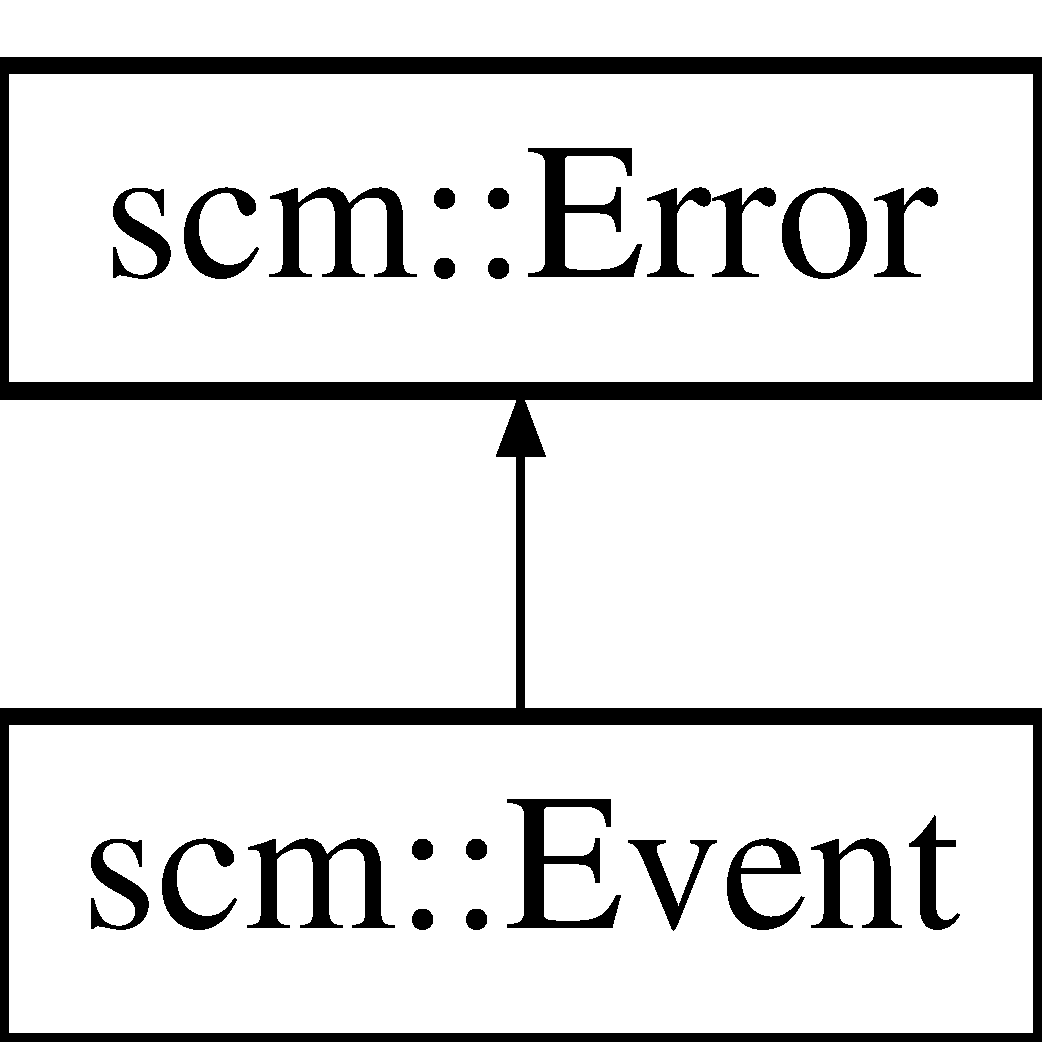
\includegraphics[height=2cm]{classscm_1_1_error}
\end{center}
\end{figure}
\subsection*{Public Member Functions}
\begin{DoxyCompactItemize}
\item 
\hyperlink{classscm_1_1_error_a9c6aa255ce180155a748f304f83830d3}{Error} (\hyperlink{namespacescm_a13a6ecf77ceb7b5b3a38e0fada54aa99}{ErrString} es)
\item 
virtual bool \hyperlink{classscm_1_1_error_a2660b73f9671be3f286bed9d622a926a}{Ok} ()=0
\item 
\hyperlink{namespacescm_a13a6ecf77ceb7b5b3a38e0fada54aa99}{ErrString} \hyperlink{classscm_1_1_error_a8fa002269b2ea7b0af4581951a7908f0}{Err} ()
\item 
void \hyperlink{classscm_1_1_error_aa4309b2556e84bd9bc6c7871f3be2f7a}{Err} (\hyperlink{namespacescm_a13a6ecf77ceb7b5b3a38e0fada54aa99}{ErrString} es)
\item 
void \hyperlink{classscm_1_1_error_a4dc4a630569665a615a0bfb321b65238}{ReportErr} ()
\item 
void \hyperlink{classscm_1_1_error_ace08c93643469a92cb3ca1e0fb1ca583}{SetReportErr} (\hyperlink{namespacescm_a13a6ecf77ceb7b5b3a38e0fada54aa99}{ErrString} es)
\item 
void \hyperlink{classscm_1_1_error_a3d3598611ee2955f3144ec2602b69677}{ClassName} (std::string cn)
\end{DoxyCompactItemize}


\subsection{Detailed Description}


Definition at line 9 of file error.h.



\subsection{Constructor \& Destructor Documentation}
\hypertarget{classscm_1_1_error_a9c6aa255ce180155a748f304f83830d3}{
\index{scm::Error@{scm::Error}!Error@{Error}}
\index{Error@{Error}!scm::Error@{scm::Error}}
\subsubsection[{Error}]{\setlength{\rightskip}{0pt plus 5cm}scm::Error::Error ({\bf ErrString} {\em es})}}
\label{classscm_1_1_error_a9c6aa255ce180155a748f304f83830d3}


Definition at line 11 of file error.cc.



\subsection{Member Function Documentation}
\hypertarget{classscm_1_1_error_a3d3598611ee2955f3144ec2602b69677}{
\index{scm::Error@{scm::Error}!ClassName@{ClassName}}
\index{ClassName@{ClassName}!scm::Error@{scm::Error}}
\subsubsection[{ClassName}]{\setlength{\rightskip}{0pt plus 5cm}void scm::Error::ClassName (std::string {\em cn})\hspace{0.3cm}{\ttfamily  \mbox{[}inline\mbox{]}}}}
\label{classscm_1_1_error_a3d3598611ee2955f3144ec2602b69677}


Definition at line 25 of file error.h.

\hypertarget{classscm_1_1_error_aa4309b2556e84bd9bc6c7871f3be2f7a}{
\index{scm::Error@{scm::Error}!Err@{Err}}
\index{Err@{Err}!scm::Error@{scm::Error}}
\subsubsection[{Err}]{\setlength{\rightskip}{0pt plus 5cm}void scm::Error::Err ({\bf scm::ErrString} {\em es})}}
\label{classscm_1_1_error_aa4309b2556e84bd9bc6c7871f3be2f7a}


Definition at line 21 of file error.cc.

\hypertarget{classscm_1_1_error_a8fa002269b2ea7b0af4581951a7908f0}{
\index{scm::Error@{scm::Error}!Err@{Err}}
\index{Err@{Err}!scm::Error@{scm::Error}}
\subsubsection[{Err}]{\setlength{\rightskip}{0pt plus 5cm}{\bf ErrString} scm::Error::Err ()}}
\label{classscm_1_1_error_a8fa002269b2ea7b0af4581951a7908f0}


Definition at line 15 of file error.cc.

\hypertarget{classscm_1_1_error_a2660b73f9671be3f286bed9d622a926a}{
\index{scm::Error@{scm::Error}!Ok@{Ok}}
\index{Ok@{Ok}!scm::Error@{scm::Error}}
\subsubsection[{Ok}]{\setlength{\rightskip}{0pt plus 5cm}virtual bool scm::Error::Ok ()\hspace{0.3cm}{\ttfamily  \mbox{[}pure virtual\mbox{]}}}}
\label{classscm_1_1_error_a2660b73f9671be3f286bed9d622a926a}


Implemented in \hyperlink{classscm_1_1_event_a95400a0d0218dfb664c028d1130a5d14}{scm::Event}.

\hypertarget{classscm_1_1_error_a4dc4a630569665a615a0bfb321b65238}{
\index{scm::Error@{scm::Error}!ReportErr@{ReportErr}}
\index{ReportErr@{ReportErr}!scm::Error@{scm::Error}}
\subsubsection[{ReportErr}]{\setlength{\rightskip}{0pt plus 5cm}void scm::Error::ReportErr ()}}
\label{classscm_1_1_error_a4dc4a630569665a615a0bfb321b65238}


Definition at line 29 of file error.cc.

\hypertarget{classscm_1_1_error_ace08c93643469a92cb3ca1e0fb1ca583}{
\index{scm::Error@{scm::Error}!SetReportErr@{SetReportErr}}
\index{SetReportErr@{SetReportErr}!scm::Error@{scm::Error}}
\subsubsection[{SetReportErr}]{\setlength{\rightskip}{0pt plus 5cm}void scm::Error::SetReportErr ({\bf ErrString} {\em es})}}
\label{classscm_1_1_error_ace08c93643469a92cb3ca1e0fb1ca583}


Definition at line 33 of file error.cc.



The documentation for this class was generated from the following files:\begin{DoxyCompactItemize}
\item 
/home/derek/dev/crml/crml/src/sys/\hyperlink{error_8h}{error.h}\item 
/home/derek/dev/crml/crml/src/sys/\hyperlink{error_8cc}{error.cc}\end{DoxyCompactItemize}

\hypertarget{classscm_1_1_event}{
\section{scm::Event Class Reference}
\label{classscm_1_1_event}\index{scm::Event@{scm::Event}}
}


{\ttfamily \#include $<$event.h$>$}

Inheritance diagram for scm::Event:\begin{figure}[H]
\begin{center}
\leavevmode
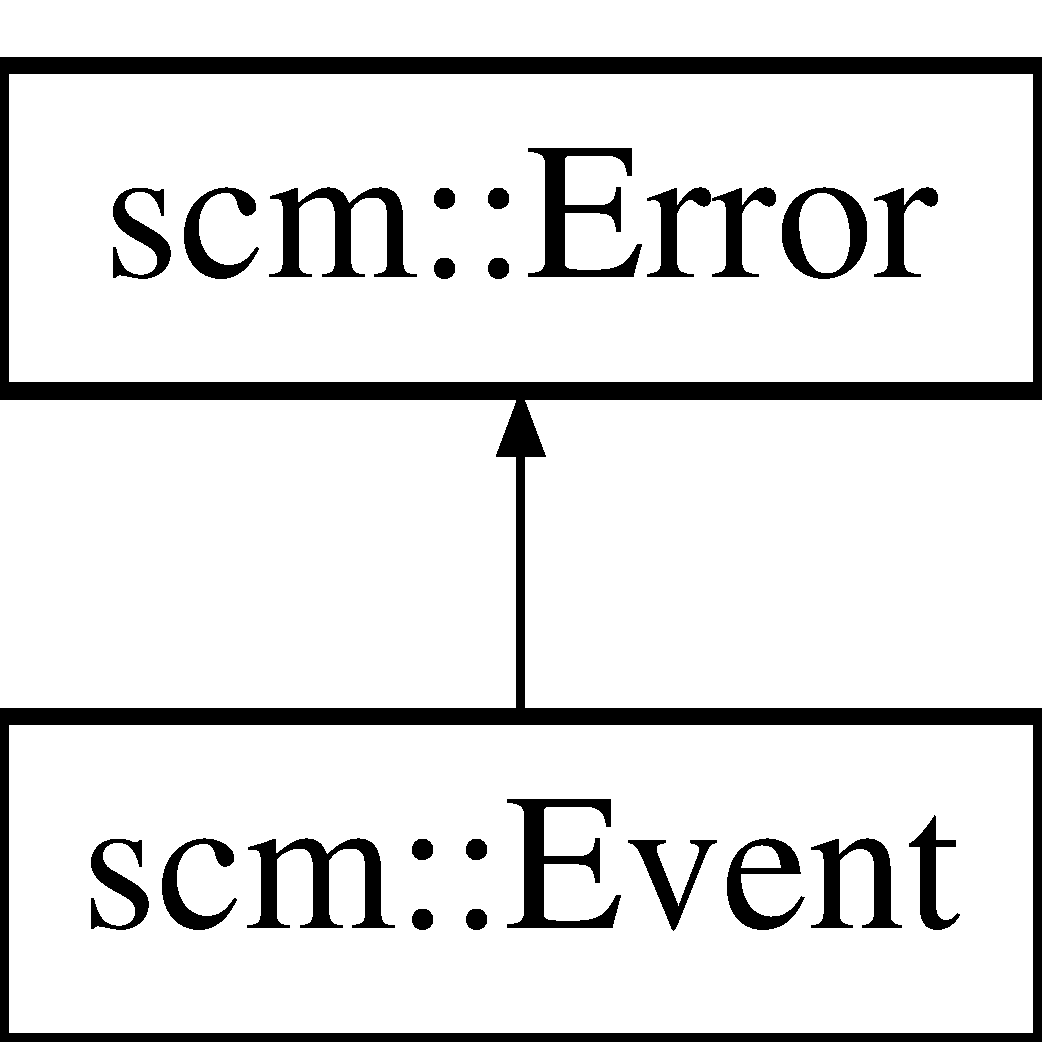
\includegraphics[height=2cm]{classscm_1_1_event}
\end{center}
\end{figure}
\subsection*{Public Member Functions}
\begin{DoxyCompactItemize}
\item 
\hyperlink{classscm_1_1_event_ae0b0fbe856c9fbce52b50e08860946e8}{Event} ()
\item 
\hyperlink{classscm_1_1_event_a4f22bf217daf2b5e3670e987579fb152}{$\sim$Event} ()
\item 
void \hyperlink{classscm_1_1_event_a2dfdf12d5b7918b2102e7ce1c4142ed3}{Init} ()
\item 
void \hyperlink{classscm_1_1_event_a1e1aa9fbe9b5e7e7c9b0ff8f0ba74cd2}{PushEvent} (\hyperlink{struct___n_p_pepper_event}{NPPepperEvent} $\ast$evt)
\item 
bool \hyperlink{classscm_1_1_event_ae736ee83efd335726cad841b6082e491}{Empty} ()
\item 
void \hyperlink{classscm_1_1_event_aba1e9492e1d03bd67afb9c8943e89fe9}{Drain} ()
\item 
\hyperlink{struct___n_p_pepper_event}{NPPepperEvent} $\ast$ \hyperlink{classscm_1_1_event_aaa7905956b3d789fa16cc7a73490dc5e}{PopEvent} ()
\item 
virtual bool \hyperlink{classscm_1_1_event_a95400a0d0218dfb664c028d1130a5d14}{Ok} ()
\end{DoxyCompactItemize}


\subsection{Detailed Description}


Definition at line 19 of file event.h.



\subsection{Constructor \& Destructor Documentation}
\hypertarget{classscm_1_1_event_ae0b0fbe856c9fbce52b50e08860946e8}{
\index{scm::Event@{scm::Event}!Event@{Event}}
\index{Event@{Event}!scm::Event@{scm::Event}}
\subsubsection[{Event}]{\setlength{\rightskip}{0pt plus 5cm}scm::Event::Event ()\hspace{0.3cm}{\ttfamily  \mbox{[}inline, explicit\mbox{]}}}}
\label{classscm_1_1_event_ae0b0fbe856c9fbce52b50e08860946e8}


Definition at line 21 of file event.h.

\hypertarget{classscm_1_1_event_a4f22bf217daf2b5e3670e987579fb152}{
\index{scm::Event@{scm::Event}!$\sim$Event@{$\sim$Event}}
\index{$\sim$Event@{$\sim$Event}!scm::Event@{scm::Event}}
\subsubsection[{$\sim$Event}]{\setlength{\rightskip}{0pt plus 5cm}scm::Event::$\sim$Event ()}}
\label{classscm_1_1_event_a4f22bf217daf2b5e3670e987579fb152}


Definition at line 17 of file event.cc.



\subsection{Member Function Documentation}
\hypertarget{classscm_1_1_event_aba1e9492e1d03bd67afb9c8943e89fe9}{
\index{scm::Event@{scm::Event}!Drain@{Drain}}
\index{Drain@{Drain}!scm::Event@{scm::Event}}
\subsubsection[{Drain}]{\setlength{\rightskip}{0pt plus 5cm}void scm::Event::Drain ()}}
\label{classscm_1_1_event_aba1e9492e1d03bd67afb9c8943e89fe9}


Definition at line 59 of file event.cc.

\hypertarget{classscm_1_1_event_ae736ee83efd335726cad841b6082e491}{
\index{scm::Event@{scm::Event}!Empty@{Empty}}
\index{Empty@{Empty}!scm::Event@{scm::Event}}
\subsubsection[{Empty}]{\setlength{\rightskip}{0pt plus 5cm}bool scm::Event::Empty ()}}
\label{classscm_1_1_event_ae736ee83efd335726cad841b6082e491}


Definition at line 26 of file event.cc.

\hypertarget{classscm_1_1_event_a2dfdf12d5b7918b2102e7ce1c4142ed3}{
\index{scm::Event@{scm::Event}!Init@{Init}}
\index{Init@{Init}!scm::Event@{scm::Event}}
\subsubsection[{Init}]{\setlength{\rightskip}{0pt plus 5cm}void scm::Event::Init ()}}
\label{classscm_1_1_event_a2dfdf12d5b7918b2102e7ce1c4142ed3}


Definition at line 21 of file event.cc.

\hypertarget{classscm_1_1_event_a95400a0d0218dfb664c028d1130a5d14}{
\index{scm::Event@{scm::Event}!Ok@{Ok}}
\index{Ok@{Ok}!scm::Event@{scm::Event}}
\subsubsection[{Ok}]{\setlength{\rightskip}{0pt plus 5cm}bool scm::Event::Ok ()\hspace{0.3cm}{\ttfamily  \mbox{[}virtual\mbox{]}}}}
\label{classscm_1_1_event_a95400a0d0218dfb664c028d1130a5d14}


Implements \hyperlink{classscm_1_1_error_a2660b73f9671be3f286bed9d622a926a}{scm::Error}.



Definition at line 13 of file event.cc.

\hypertarget{classscm_1_1_event_aaa7905956b3d789fa16cc7a73490dc5e}{
\index{scm::Event@{scm::Event}!PopEvent@{PopEvent}}
\index{PopEvent@{PopEvent}!scm::Event@{scm::Event}}
\subsubsection[{PopEvent}]{\setlength{\rightskip}{0pt plus 5cm}{\bf NPPepperEvent} $\ast$ scm::Event::PopEvent ()}}
\label{classscm_1_1_event_aaa7905956b3d789fa16cc7a73490dc5e}


Definition at line 50 of file event.cc.

\hypertarget{classscm_1_1_event_a1e1aa9fbe9b5e7e7c9b0ff8f0ba74cd2}{
\index{scm::Event@{scm::Event}!PushEvent@{PushEvent}}
\index{PushEvent@{PushEvent}!scm::Event@{scm::Event}}
\subsubsection[{PushEvent}]{\setlength{\rightskip}{0pt plus 5cm}void scm::Event::PushEvent ({\bf NPPepperEvent} $\ast$ {\em evt})}}
\label{classscm_1_1_event_a1e1aa9fbe9b5e7e7c9b0ff8f0ba74cd2}


Definition at line 65 of file event.cc.



The documentation for this class was generated from the following files:\begin{DoxyCompactItemize}
\item 
/home/derek/dev/cell-\/grid-\/game/nacl/crml/crml/evt/\hyperlink{event_8h}{event.h}\item 
/home/derek/dev/cell-\/grid-\/game/nacl/crml/crml/evt/\hyperlink{event_8cc}{event.cc}\end{DoxyCompactItemize}

\hypertarget{class_event_handler}{
\section{EventHandler Class Reference}
\label{class_event_handler}\index{EventHandler@{EventHandler}}
}


{\ttfamily \#include $<$event\_\-handler.h$>$}

\subsection*{Public Member Functions}
\begin{DoxyCompactItemize}
\item 
\hyperlink{class_event_handler_a6b7f9af8b5c3c4128047d35467ca0da0}{EventHandler} (\hyperlink{struct___n_p_p}{NPP} npp)
\item 
\hyperlink{class_event_handler_a3decb8cd88ba8af2b9b0b0f0f2fcd722}{$\sim$EventHandler} ()
\item 
bool \hyperlink{class_event_handler_a18771c6be120edf9d912a4003066b8b3}{addText} (const char $\ast$cstr)
\item 
int \hyperlink{class_event_handler_a2fcafd6f528017d8a814f9c384e2e057}{handle} (void $\ast$event)
\item 
bool \hyperlink{class_event_handler_a2f334e3eb39be72751e342619489e695}{is\_\-text\_\-box\_\-set} ()
\item 
bool \hyperlink{class_event_handler_aa09c0b995aa6c774d4a33be13be0cbf2}{set\_\-text\_\-box} (NPObject $\ast$text\_\-box\_\-object)
\item 
void \hyperlink{class_event_handler_a67d149352861c0a8fe603a14585d1003}{Init} (\hyperlink{classscm_1_1_event}{scm::Event} $\ast$)
\end{DoxyCompactItemize}


\subsection{Detailed Description}


Definition at line 34 of file event\_\-handler.h.



\subsection{Constructor \& Destructor Documentation}
\hypertarget{class_event_handler_a6b7f9af8b5c3c4128047d35467ca0da0}{
\index{EventHandler@{EventHandler}!EventHandler@{EventHandler}}
\index{EventHandler@{EventHandler}!EventHandler@{EventHandler}}
\subsubsection[{EventHandler}]{\setlength{\rightskip}{0pt plus 5cm}EventHandler::EventHandler ({\bf NPP} {\em npp})\hspace{0.3cm}{\ttfamily  \mbox{[}explicit\mbox{]}}}}
\label{class_event_handler_a6b7f9af8b5c3c4128047d35467ca0da0}


Definition at line 57 of file event\_\-handler.cc.

\hypertarget{class_event_handler_a3decb8cd88ba8af2b9b0b0f0f2fcd722}{
\index{EventHandler@{EventHandler}!$\sim$EventHandler@{$\sim$EventHandler}}
\index{$\sim$EventHandler@{$\sim$EventHandler}!EventHandler@{EventHandler}}
\subsubsection[{$\sim$EventHandler}]{\setlength{\rightskip}{0pt plus 5cm}EventHandler::$\sim$EventHandler ()}}
\label{class_event_handler_a3decb8cd88ba8af2b9b0b0f0f2fcd722}


Definition at line 62 of file event\_\-handler.cc.



\subsection{Member Function Documentation}
\hypertarget{class_event_handler_a18771c6be120edf9d912a4003066b8b3}{
\index{EventHandler@{EventHandler}!addText@{addText}}
\index{addText@{addText}!EventHandler@{EventHandler}}
\subsubsection[{addText}]{\setlength{\rightskip}{0pt plus 5cm}bool EventHandler::addText (const char $\ast$ {\em cstr})}}
\label{class_event_handler_a18771c6be120edf9d912a4003066b8b3}


Definition at line 71 of file event\_\-handler.cc.

\hypertarget{class_event_handler_a2fcafd6f528017d8a814f9c384e2e057}{
\index{EventHandler@{EventHandler}!handle@{handle}}
\index{handle@{handle}!EventHandler@{EventHandler}}
\subsubsection[{handle}]{\setlength{\rightskip}{0pt plus 5cm}int EventHandler::handle (void $\ast$ {\em event})}}
\label{class_event_handler_a2fcafd6f528017d8a814f9c384e2e057}


Definition at line 121 of file event\_\-handler.cc.

\hypertarget{class_event_handler_a67d149352861c0a8fe603a14585d1003}{
\index{EventHandler@{EventHandler}!Init@{Init}}
\index{Init@{Init}!EventHandler@{EventHandler}}
\subsubsection[{Init}]{\setlength{\rightskip}{0pt plus 5cm}void EventHandler::Init ({\bf scm::Event} $\ast$ {\em sys})}}
\label{class_event_handler_a67d149352861c0a8fe603a14585d1003}


Definition at line 65 of file event\_\-handler.cc.

\hypertarget{class_event_handler_a2f334e3eb39be72751e342619489e695}{
\index{EventHandler@{EventHandler}!is\_\-text\_\-box\_\-set@{is\_\-text\_\-box\_\-set}}
\index{is\_\-text\_\-box\_\-set@{is\_\-text\_\-box\_\-set}!EventHandler@{EventHandler}}
\subsubsection[{is\_\-text\_\-box\_\-set}]{\setlength{\rightskip}{0pt plus 5cm}bool EventHandler::is\_\-text\_\-box\_\-set ()}}
\label{class_event_handler_a2f334e3eb39be72751e342619489e695}


Definition at line 187 of file event\_\-handler.cc.

\hypertarget{class_event_handler_aa09c0b995aa6c774d4a33be13be0cbf2}{
\index{EventHandler@{EventHandler}!set\_\-text\_\-box@{set\_\-text\_\-box}}
\index{set\_\-text\_\-box@{set\_\-text\_\-box}!EventHandler@{EventHandler}}
\subsubsection[{set\_\-text\_\-box}]{\setlength{\rightskip}{0pt plus 5cm}bool EventHandler::set\_\-text\_\-box (NPObject $\ast$ {\em text\_\-box\_\-object})}}
\label{class_event_handler_aa09c0b995aa6c774d4a33be13be0cbf2}


Definition at line 193 of file event\_\-handler.cc.



The documentation for this class was generated from the following files:\begin{DoxyCompactItemize}
\item 
/home/derek/dev/cell-\/grid-\/game/nacl/crml/crml/evt/\hyperlink{event__handler_8h}{event\_\-handler.h}\item 
/home/derek/dev/cell-\/grid-\/game/nacl/crml/crml/evt/\hyperlink{event__handler_8cc}{event\_\-handler.cc}\end{DoxyCompactItemize}

\hypertarget{struct_hello_world}{
\section{HelloWorld Struct Reference}
\label{struct_hello_world}\index{HelloWorld@{HelloWorld}}
}
\subsection*{Public Attributes}
\begin{DoxyCompactItemize}
\item 
\hyperlink{struct___n_p_p}{NPP} \hyperlink{struct_hello_world_a8546fa606713a22cd373527986469eba}{npp}
\item 
\hyperlink{struct_n_p_object}{NPObject} $\ast$ \hyperlink{struct_hello_world_ab53916603277423408f4e4997b3b5733}{npobject}
\end{DoxyCompactItemize}


\subsection{Detailed Description}


Definition at line 13 of file npp\_\-gate.cc.



\subsection{Member Data Documentation}
\hypertarget{struct_hello_world_ab53916603277423408f4e4997b3b5733}{
\index{HelloWorld@{HelloWorld}!npobject@{npobject}}
\index{npobject@{npobject}!HelloWorld@{HelloWorld}}
\subsubsection[{npobject}]{\setlength{\rightskip}{0pt plus 5cm}{\bf NPObject}$\ast$ {\bf HelloWorld::npobject}}}
\label{struct_hello_world_ab53916603277423408f4e4997b3b5733}


Definition at line 15 of file npp\_\-gate.cc.

\hypertarget{struct_hello_world_a8546fa606713a22cd373527986469eba}{
\index{HelloWorld@{HelloWorld}!npp@{npp}}
\index{npp@{npp}!HelloWorld@{HelloWorld}}
\subsubsection[{npp}]{\setlength{\rightskip}{0pt plus 5cm}{\bf NPP} {\bf HelloWorld::npp}}}
\label{struct_hello_world_a8546fa606713a22cd373527986469eba}


Definition at line 14 of file npp\_\-gate.cc.



The documentation for this struct was generated from the following file:\begin{DoxyCompactItemize}
\item 
/home/derek/dev/cell-\/grid-\/game/nacl/crml/crml/sys/\hyperlink{sys_2npp__gate_8cc}{npp\_\-gate.cc}\end{DoxyCompactItemize}

\hypertarget{class_hello_world_instance}{
\section{HelloWorldInstance Class Reference}
\label{class_hello_world_instance}\index{HelloWorldInstance@{HelloWorldInstance}}
}
\subsection*{Public Member Functions}
\begin{DoxyCompactItemize}
\item 
\hyperlink{class_hello_world_instance_add03eac81a09900135582a464bfcd8f8}{HelloWorldInstance} (PP\_\-Instance instance)
\item 
virtual \hyperlink{class_hello_world_instance_ab82a0f1aa35b3f8fbc2e107af026bfc5}{$\sim$HelloWorldInstance} ()
\item 
virtual pp::Var \hyperlink{class_hello_world_instance_ac489a6775aead72dc1b17d22d1eb6688}{GetInstanceObject} ()
\end{DoxyCompactItemize}


\subsection{Detailed Description}


Definition at line 102 of file hello\_\-world.cc.



\subsection{Constructor \& Destructor Documentation}
\hypertarget{class_hello_world_instance_add03eac81a09900135582a464bfcd8f8}{
\index{HelloWorldInstance@{HelloWorldInstance}!HelloWorldInstance@{HelloWorldInstance}}
\index{HelloWorldInstance@{HelloWorldInstance}!HelloWorldInstance@{HelloWorldInstance}}
\subsubsection[{HelloWorldInstance}]{\setlength{\rightskip}{0pt plus 5cm}HelloWorldInstance::HelloWorldInstance (PP\_\-Instance {\em instance})\hspace{0.3cm}{\ttfamily  \mbox{[}inline\mbox{]}}}}
\label{class_hello_world_instance_add03eac81a09900135582a464bfcd8f8}


Definition at line 104 of file hello\_\-world.cc.

\hypertarget{class_hello_world_instance_ab82a0f1aa35b3f8fbc2e107af026bfc5}{
\index{HelloWorldInstance@{HelloWorldInstance}!$\sim$HelloWorldInstance@{$\sim$HelloWorldInstance}}
\index{$\sim$HelloWorldInstance@{$\sim$HelloWorldInstance}!HelloWorldInstance@{HelloWorldInstance}}
\subsubsection[{$\sim$HelloWorldInstance}]{\setlength{\rightskip}{0pt plus 5cm}virtual HelloWorldInstance::$\sim$HelloWorldInstance ()\hspace{0.3cm}{\ttfamily  \mbox{[}inline, virtual\mbox{]}}}}
\label{class_hello_world_instance_ab82a0f1aa35b3f8fbc2e107af026bfc5}


Definition at line 105 of file hello\_\-world.cc.



\subsection{Member Function Documentation}
\hypertarget{class_hello_world_instance_ac489a6775aead72dc1b17d22d1eb6688}{
\index{HelloWorldInstance@{HelloWorldInstance}!GetInstanceObject@{GetInstanceObject}}
\index{GetInstanceObject@{GetInstanceObject}!HelloWorldInstance@{HelloWorldInstance}}
\subsubsection[{GetInstanceObject}]{\setlength{\rightskip}{0pt plus 5cm}virtual pp::Var HelloWorldInstance::GetInstanceObject ()\hspace{0.3cm}{\ttfamily  \mbox{[}inline, virtual\mbox{]}}}}
\label{class_hello_world_instance_ac489a6775aead72dc1b17d22d1eb6688}


Definition at line 108 of file hello\_\-world.cc.



The documentation for this class was generated from the following file:\begin{DoxyCompactItemize}
\item 
/home/derek/dev/crml/crml/test/hello\_\-world/\hyperlink{hello__world_8cc}{hello\_\-world.cc}\end{DoxyCompactItemize}

\hypertarget{class_hello_world_module}{
\section{HelloWorldModule Class Reference}
\label{class_hello_world_module}\index{HelloWorldModule@{HelloWorldModule}}
}
\subsection*{Public Member Functions}
\begin{DoxyCompactItemize}
\item 
\hyperlink{class_hello_world_module_a51bebf2cbff1d8914b988101781bd01d}{HelloWorldModule} ()
\item 
virtual \hyperlink{class_hello_world_module_a2458f9ee6a26568e54c6bd3a0323abcf}{$\sim$HelloWorldModule} ()
\item 
virtual pp::Instance $\ast$ \hyperlink{class_hello_world_module_a6ee0eeeb3ed2f95b819adfd4df33c47f}{CreateInstance} (PP\_\-Instance instance)
\end{DoxyCompactItemize}


\subsection{Detailed Description}


Definition at line 117 of file hello\_\-world.cc.



\subsection{Constructor \& Destructor Documentation}
\hypertarget{class_hello_world_module_a51bebf2cbff1d8914b988101781bd01d}{
\index{HelloWorldModule@{HelloWorldModule}!HelloWorldModule@{HelloWorldModule}}
\index{HelloWorldModule@{HelloWorldModule}!HelloWorldModule@{HelloWorldModule}}
\subsubsection[{HelloWorldModule}]{\setlength{\rightskip}{0pt plus 5cm}HelloWorldModule::HelloWorldModule ()\hspace{0.3cm}{\ttfamily  \mbox{[}inline\mbox{]}}}}
\label{class_hello_world_module_a51bebf2cbff1d8914b988101781bd01d}


Definition at line 119 of file hello\_\-world.cc.

\hypertarget{class_hello_world_module_a2458f9ee6a26568e54c6bd3a0323abcf}{
\index{HelloWorldModule@{HelloWorldModule}!$\sim$HelloWorldModule@{$\sim$HelloWorldModule}}
\index{$\sim$HelloWorldModule@{$\sim$HelloWorldModule}!HelloWorldModule@{HelloWorldModule}}
\subsubsection[{$\sim$HelloWorldModule}]{\setlength{\rightskip}{0pt plus 5cm}virtual HelloWorldModule::$\sim$HelloWorldModule ()\hspace{0.3cm}{\ttfamily  \mbox{[}inline, virtual\mbox{]}}}}
\label{class_hello_world_module_a2458f9ee6a26568e54c6bd3a0323abcf}


Definition at line 120 of file hello\_\-world.cc.



\subsection{Member Function Documentation}
\hypertarget{class_hello_world_module_a6ee0eeeb3ed2f95b819adfd4df33c47f}{
\index{HelloWorldModule@{HelloWorldModule}!CreateInstance@{CreateInstance}}
\index{CreateInstance@{CreateInstance}!HelloWorldModule@{HelloWorldModule}}
\subsubsection[{CreateInstance}]{\setlength{\rightskip}{0pt plus 5cm}virtual pp::Instance$\ast$ HelloWorldModule::CreateInstance (PP\_\-Instance {\em instance})\hspace{0.3cm}{\ttfamily  \mbox{[}inline, virtual\mbox{]}}}}
\label{class_hello_world_module_a6ee0eeeb3ed2f95b819adfd4df33c47f}


Definition at line 123 of file hello\_\-world.cc.



The documentation for this class was generated from the following file:\begin{DoxyCompactItemize}
\item 
/home/derek/dev/cell-\/grid-\/game/nacl/crml/crml/test/hello\_\-world/\hyperlink{hello__world_8cc}{hello\_\-world.cc}\end{DoxyCompactItemize}

\hypertarget{class_hello_world_scriptable_object}{
\section{HelloWorldScriptableObject Class Reference}
\label{class_hello_world_scriptable_object}\index{HelloWorldScriptableObject@{HelloWorldScriptableObject}}
}
\subsection*{Public Member Functions}
\begin{DoxyCompactItemize}
\item 
virtual bool \hyperlink{class_hello_world_scriptable_object_a0af23165c74483e47f97877cbb51e79a}{HasMethod} (const pp::Var \&method, pp::Var $\ast$exception)
\item 
virtual pp::Var \hyperlink{class_hello_world_scriptable_object_a217b4b958a4bfb250dd8ac588ab794ad}{Call} (const pp::Var \&method, const std::vector$<$ pp::Var $>$ \&args, pp::Var $\ast$exception)
\end{DoxyCompactItemize}


\subsection{Detailed Description}


Definition at line 53 of file hello\_\-world.cc.



\subsection{Member Function Documentation}
\hypertarget{class_hello_world_scriptable_object_a217b4b958a4bfb250dd8ac588ab794ad}{
\index{HelloWorldScriptableObject@{HelloWorldScriptableObject}!Call@{Call}}
\index{Call@{Call}!HelloWorldScriptableObject@{HelloWorldScriptableObject}}
\subsubsection[{Call}]{\setlength{\rightskip}{0pt plus 5cm}pp::Var HelloWorldScriptableObject::Call (const pp::Var \& {\em method}, \/  const std::vector$<$ pp::Var $>$ \& {\em args}, \/  pp::Var $\ast$ {\em exception})\hspace{0.3cm}{\ttfamily  \mbox{[}virtual\mbox{]}}}}
\label{class_hello_world_scriptable_object_a217b4b958a4bfb250dd8ac588ab794ad}


Definition at line 77 of file hello\_\-world.cc.

\hypertarget{class_hello_world_scriptable_object_a0af23165c74483e47f97877cbb51e79a}{
\index{HelloWorldScriptableObject@{HelloWorldScriptableObject}!HasMethod@{HasMethod}}
\index{HasMethod@{HasMethod}!HelloWorldScriptableObject@{HelloWorldScriptableObject}}
\subsubsection[{HasMethod}]{\setlength{\rightskip}{0pt plus 5cm}bool HelloWorldScriptableObject::HasMethod (const pp::Var \& {\em method}, \/  pp::Var $\ast$ {\em exception})\hspace{0.3cm}{\ttfamily  \mbox{[}virtual\mbox{]}}}}
\label{class_hello_world_scriptable_object_a0af23165c74483e47f97877cbb51e79a}


Definition at line 66 of file hello\_\-world.cc.



The documentation for this class was generated from the following file:\begin{DoxyCompactItemize}
\item 
/home/derek/dev/cell-\/grid-\/game/nacl/crml/crml/test/hello\_\-world/\hyperlink{hello__world_8cc}{hello\_\-world.cc}\end{DoxyCompactItemize}

\hypertarget{classscm_1_1_hex_store}{
\section{scm::HexStore Class Reference}
\label{classscm_1_1_hex_store}\index{scm::HexStore@{scm::HexStore}}
}


{\ttfamily \#include $<$hex\_\-store.h$>$}

\subsection*{Public Member Functions}
\begin{DoxyCompactItemize}
\item 
\hyperlink{classscm_1_1_hex_store_ae3ea77bf45ef55916e02aba5f5d280f5}{HexStore} ()
\item 
\hyperlink{classscm_1_1_hex_store_ac418965e7e9ee7569bb03b7230bad1bd}{$\sim$HexStore} ()
\item 
bool \hyperlink{classscm_1_1_hex_store_ae8d894818fe0859462b63f2e34d08a33}{Ok} ()
\item 
int \hyperlink{classscm_1_1_hex_store_a85cbfdc7f9a41355db174d3b96382d79}{Err} ()
\item 
void \hyperlink{classscm_1_1_hex_store_ac98d4c0f37c642e6b45262ec1db62d80}{ReportErr} ()
\item 
void \hyperlink{classscm_1_1_hex_store_aa1792118dbb32383976d6906c69c9e71}{Store} (std::string, std::string)
\item 
int \hyperlink{classscm_1_1_hex_store_a277a7c2220511ad3c0e447802589def1}{ValLength} (std::string)
\item 
bool \hyperlink{classscm_1_1_hex_store_a2c7a1fc73741e0b3613516388b562475}{EmptyVal} (std::string)
\item 
void \hyperlink{classscm_1_1_hex_store_ac086449d331c2e0dd6eaf11a003ffe99}{Append} (std::string, std::string)
\item 
std::string \hyperlink{classscm_1_1_hex_store_acdc20757093a52e3f7748dea41d185b2}{GetValue} (std::string)
\item 
const char $\ast$ \hyperlink{classscm_1_1_hex_store_a5e12c88428e17be9bb8f6c08ab107e57}{ByteArray} (std::string)
\end{DoxyCompactItemize}


\subsection{Detailed Description}


Definition at line 19 of file hex\_\-store.h.



\subsection{Constructor \& Destructor Documentation}
\hypertarget{classscm_1_1_hex_store_ae3ea77bf45ef55916e02aba5f5d280f5}{
\index{scm::HexStore@{scm::HexStore}!HexStore@{HexStore}}
\index{HexStore@{HexStore}!scm::HexStore@{scm::HexStore}}
\subsubsection[{HexStore}]{\setlength{\rightskip}{0pt plus 5cm}scm::HexStore::HexStore ()}}
\label{classscm_1_1_hex_store_ae3ea77bf45ef55916e02aba5f5d280f5}


Definition at line 11 of file hex\_\-store.cc.

\hypertarget{classscm_1_1_hex_store_ac418965e7e9ee7569bb03b7230bad1bd}{
\index{scm::HexStore@{scm::HexStore}!$\sim$HexStore@{$\sim$HexStore}}
\index{$\sim$HexStore@{$\sim$HexStore}!scm::HexStore@{scm::HexStore}}
\subsubsection[{$\sim$HexStore}]{\setlength{\rightskip}{0pt plus 5cm}scm::HexStore::$\sim$HexStore ()}}
\label{classscm_1_1_hex_store_ac418965e7e9ee7569bb03b7230bad1bd}


Definition at line 12 of file hex\_\-store.cc.



\subsection{Member Function Documentation}
\hypertarget{classscm_1_1_hex_store_ac086449d331c2e0dd6eaf11a003ffe99}{
\index{scm::HexStore@{scm::HexStore}!Append@{Append}}
\index{Append@{Append}!scm::HexStore@{scm::HexStore}}
\subsubsection[{Append}]{\setlength{\rightskip}{0pt plus 5cm}void scm::HexStore::Append (std::string {\em key}, \/  std::string {\em val})}}
\label{classscm_1_1_hex_store_ac086449d331c2e0dd6eaf11a003ffe99}


Definition at line 67 of file hex\_\-store.cc.

\hypertarget{classscm_1_1_hex_store_a5e12c88428e17be9bb8f6c08ab107e57}{
\index{scm::HexStore@{scm::HexStore}!ByteArray@{ByteArray}}
\index{ByteArray@{ByteArray}!scm::HexStore@{scm::HexStore}}
\subsubsection[{ByteArray}]{\setlength{\rightskip}{0pt plus 5cm}const char $\ast$ scm::HexStore::ByteArray (std::string {\em key})}}
\label{classscm_1_1_hex_store_a5e12c88428e17be9bb8f6c08ab107e57}


Definition at line 79 of file hex\_\-store.cc.

\hypertarget{classscm_1_1_hex_store_a2c7a1fc73741e0b3613516388b562475}{
\index{scm::HexStore@{scm::HexStore}!EmptyVal@{EmptyVal}}
\index{EmptyVal@{EmptyVal}!scm::HexStore@{scm::HexStore}}
\subsubsection[{EmptyVal}]{\setlength{\rightskip}{0pt plus 5cm}bool scm::HexStore::EmptyVal (std::string {\em key})}}
\label{classscm_1_1_hex_store_a2c7a1fc73741e0b3613516388b562475}


Definition at line 45 of file hex\_\-store.cc.

\hypertarget{classscm_1_1_hex_store_a85cbfdc7f9a41355db174d3b96382d79}{
\index{scm::HexStore@{scm::HexStore}!Err@{Err}}
\index{Err@{Err}!scm::HexStore@{scm::HexStore}}
\subsubsection[{Err}]{\setlength{\rightskip}{0pt plus 5cm}int scm::HexStore::Err ()}}
\label{classscm_1_1_hex_store_a85cbfdc7f9a41355db174d3b96382d79}


Definition at line 15 of file hex\_\-store.cc.

\hypertarget{classscm_1_1_hex_store_acdc20757093a52e3f7748dea41d185b2}{
\index{scm::HexStore@{scm::HexStore}!GetValue@{GetValue}}
\index{GetValue@{GetValue}!scm::HexStore@{scm::HexStore}}
\subsubsection[{GetValue}]{\setlength{\rightskip}{0pt plus 5cm}std::string scm::HexStore::GetValue (std::string {\em key})}}
\label{classscm_1_1_hex_store_acdc20757093a52e3f7748dea41d185b2}


Definition at line 58 of file hex\_\-store.cc.

\hypertarget{classscm_1_1_hex_store_ae8d894818fe0859462b63f2e34d08a33}{
\index{scm::HexStore@{scm::HexStore}!Ok@{Ok}}
\index{Ok@{Ok}!scm::HexStore@{scm::HexStore}}
\subsubsection[{Ok}]{\setlength{\rightskip}{0pt plus 5cm}bool scm::HexStore::Ok ()}}
\label{classscm_1_1_hex_store_ae8d894818fe0859462b63f2e34d08a33}


Definition at line 19 of file hex\_\-store.cc.

\hypertarget{classscm_1_1_hex_store_ac98d4c0f37c642e6b45262ec1db62d80}{
\index{scm::HexStore@{scm::HexStore}!ReportErr@{ReportErr}}
\index{ReportErr@{ReportErr}!scm::HexStore@{scm::HexStore}}
\subsubsection[{ReportErr}]{\setlength{\rightskip}{0pt plus 5cm}void scm::HexStore::ReportErr ()}}
\label{classscm_1_1_hex_store_ac98d4c0f37c642e6b45262ec1db62d80}


Definition at line 23 of file hex\_\-store.cc.

\hypertarget{classscm_1_1_hex_store_aa1792118dbb32383976d6906c69c9e71}{
\index{scm::HexStore@{scm::HexStore}!Store@{Store}}
\index{Store@{Store}!scm::HexStore@{scm::HexStore}}
\subsubsection[{Store}]{\setlength{\rightskip}{0pt plus 5cm}void scm::HexStore::Store (std::string {\em key}, \/  std::string {\em val})}}
\label{classscm_1_1_hex_store_aa1792118dbb32383976d6906c69c9e71}


Definition at line 40 of file hex\_\-store.cc.

\hypertarget{classscm_1_1_hex_store_a277a7c2220511ad3c0e447802589def1}{
\index{scm::HexStore@{scm::HexStore}!ValLength@{ValLength}}
\index{ValLength@{ValLength}!scm::HexStore@{scm::HexStore}}
\subsubsection[{ValLength}]{\setlength{\rightskip}{0pt plus 5cm}int scm::HexStore::ValLength (std::string {\em key})}}
\label{classscm_1_1_hex_store_a277a7c2220511ad3c0e447802589def1}


Definition at line 49 of file hex\_\-store.cc.



The documentation for this class was generated from the following files:\begin{DoxyCompactItemize}
\item 
/home/derek/dev/cell-\/grid-\/game/nacl/crml/crml/sys/\hyperlink{hex__store_8h}{hex\_\-store.h}\item 
/home/derek/dev/cell-\/grid-\/game/nacl/crml/crml/sys/\hyperlink{hex__store_8cc}{hex\_\-store.cc}\end{DoxyCompactItemize}

\hypertarget{classscm_1_1_mainloop}{
\section{scm::Mainloop Class Reference}
\label{classscm_1_1_mainloop}\index{scm::Mainloop@{scm::Mainloop}}
}


{\ttfamily \#include $<$loop.h$>$}

\subsection*{Public Member Functions}
\begin{DoxyCompactItemize}
\item 
\hyperlink{classscm_1_1_mainloop_abacbb3c174abded439ddf745e840dd29}{Mainloop} ()
\item 
\hyperlink{classscm_1_1_mainloop_a0638591ae4a2df7e99d2ba586ad5edfe}{$\sim$Mainloop} ()
\item 
void \hyperlink{classscm_1_1_mainloop_a7e332605f463847553999278a975d650}{Go} ()
\item 
\hyperlink{namespacescm_aec9fbdb87d677e6e822d612ed3e3a20b}{MainloopErr} \hyperlink{classscm_1_1_mainloop_a47a4747a4529b29b2337942496bc4e61}{SetFramesPerSecond} (double)
\item 
\hyperlink{namespacescm_aec9fbdb87d677e6e822d612ed3e3a20b}{MainloopErr} \hyperlink{classscm_1_1_mainloop_a3b4177ac538fb42bc7bed6bb5e84a6dc}{Init} (\hyperlink{class_plugin_object}{PluginObject} $\ast$)
\item 
\hyperlink{namespacescm_aec9fbdb87d677e6e822d612ed3e3a20b}{MainloopErr} \hyperlink{classscm_1_1_mainloop_ab4e2e2a9df321c2761d24690a503cc06}{Init2D} (NPDevice $\ast$)
\end{DoxyCompactItemize}


\subsection{Detailed Description}


Definition at line 19 of file loop.h.



\subsection{Constructor \& Destructor Documentation}
\hypertarget{classscm_1_1_mainloop_abacbb3c174abded439ddf745e840dd29}{
\index{scm::Mainloop@{scm::Mainloop}!Mainloop@{Mainloop}}
\index{Mainloop@{Mainloop}!scm::Mainloop@{scm::Mainloop}}
\subsubsection[{Mainloop}]{\setlength{\rightskip}{0pt plus 5cm}scm::Mainloop::Mainloop ()}}
\label{classscm_1_1_mainloop_abacbb3c174abded439ddf745e840dd29}


Definition at line 6 of file loop.cc.

\hypertarget{classscm_1_1_mainloop_a0638591ae4a2df7e99d2ba586ad5edfe}{
\index{scm::Mainloop@{scm::Mainloop}!$\sim$Mainloop@{$\sim$Mainloop}}
\index{$\sim$Mainloop@{$\sim$Mainloop}!scm::Mainloop@{scm::Mainloop}}
\subsubsection[{$\sim$Mainloop}]{\setlength{\rightskip}{0pt plus 5cm}scm::Mainloop::$\sim$Mainloop ()}}
\label{classscm_1_1_mainloop_a0638591ae4a2df7e99d2ba586ad5edfe}


Definition at line 12 of file loop.cc.



\subsection{Member Function Documentation}
\hypertarget{classscm_1_1_mainloop_a7e332605f463847553999278a975d650}{
\index{scm::Mainloop@{scm::Mainloop}!Go@{Go}}
\index{Go@{Go}!scm::Mainloop@{scm::Mainloop}}
\subsubsection[{Go}]{\setlength{\rightskip}{0pt plus 5cm}void scm::Mainloop::Go ()}}
\label{classscm_1_1_mainloop_a7e332605f463847553999278a975d650}


Definition at line 23 of file loop.cc.

\hypertarget{classscm_1_1_mainloop_a3b4177ac538fb42bc7bed6bb5e84a6dc}{
\index{scm::Mainloop@{scm::Mainloop}!Init@{Init}}
\index{Init@{Init}!scm::Mainloop@{scm::Mainloop}}
\subsubsection[{Init}]{\setlength{\rightskip}{0pt plus 5cm}{\bf MainloopErr} scm::Mainloop::Init ({\bf PluginObject} $\ast$ {\em po})}}
\label{classscm_1_1_mainloop_a3b4177ac538fb42bc7bed6bb5e84a6dc}


Definition at line 53 of file loop.cc.

\hypertarget{classscm_1_1_mainloop_ab4e2e2a9df321c2761d24690a503cc06}{
\index{scm::Mainloop@{scm::Mainloop}!Init2D@{Init2D}}
\index{Init2D@{Init2D}!scm::Mainloop@{scm::Mainloop}}
\subsubsection[{Init2D}]{\setlength{\rightskip}{0pt plus 5cm}{\bf MainloopErr} scm::Mainloop::Init2D (NPDevice $\ast$ {\em device2d})}}
\label{classscm_1_1_mainloop_ab4e2e2a9df321c2761d24690a503cc06}


Definition at line 39 of file loop.cc.

\hypertarget{classscm_1_1_mainloop_a47a4747a4529b29b2337942496bc4e61}{
\index{scm::Mainloop@{scm::Mainloop}!SetFramesPerSecond@{SetFramesPerSecond}}
\index{SetFramesPerSecond@{SetFramesPerSecond}!scm::Mainloop@{scm::Mainloop}}
\subsubsection[{SetFramesPerSecond}]{\setlength{\rightskip}{0pt plus 5cm}{\bf MainloopErr} scm::Mainloop::SetFramesPerSecond (double {\em fps})}}
\label{classscm_1_1_mainloop_a47a4747a4529b29b2337942496bc4e61}


Definition at line 47 of file loop.cc.



The documentation for this class was generated from the following files:\begin{DoxyCompactItemize}
\item 
/home/derek/dev/cell-\/grid-\/game/nacl/crml/crml/sys/\hyperlink{loop_8h}{loop.h}\item 
/home/derek/dev/cell-\/grid-\/game/nacl/crml/crml/sys/\hyperlink{loop_8cc}{loop.cc}\end{DoxyCompactItemize}

\hypertarget{struct_m_d5_digest__struct}{
\section{MD5Digest\_\-struct Struct Reference}
\label{struct_m_d5_digest__struct}\index{MD5Digest\_\-struct@{MD5Digest\_\-struct}}
}


{\ttfamily \#include $<$md5.h$>$}

\subsection*{Public Attributes}
\begin{DoxyCompactItemize}
\item 
unsigned char \hyperlink{struct_m_d5_digest__struct_a47ba426c0b835e8947717e860464b255}{a} \mbox{[}16\mbox{]}
\end{DoxyCompactItemize}


\subsection{Detailed Description}


Definition at line 34 of file md5.h.



\subsection{Member Data Documentation}
\hypertarget{struct_m_d5_digest__struct_a47ba426c0b835e8947717e860464b255}{
\index{MD5Digest\_\-struct@{MD5Digest\_\-struct}!a@{a}}
\index{a@{a}!MD5Digest_struct@{MD5Digest\_\-struct}}
\subsubsection[{a}]{\setlength{\rightskip}{0pt plus 5cm}unsigned char {\bf MD5Digest\_\-struct::a}\mbox{[}16\mbox{]}}}
\label{struct_m_d5_digest__struct_a47ba426c0b835e8947717e860464b255}


Definition at line 35 of file md5.h.



The documentation for this struct was generated from the following file:\begin{DoxyCompactItemize}
\item 
/home/derek/dev/cell-\/grid-\/game/nacl/crml/crml/sys/\hyperlink{md5_8h}{md5.h}\end{DoxyCompactItemize}

\hypertarget{struct_n_p_class}{
\section{NPClass Struct Reference}
\label{struct_n_p_class}\index{NPClass@{NPClass}}
}


{\ttfamily \#include $<$npruntime.h$>$}

\subsection*{Public Attributes}
\begin{DoxyCompactItemize}
\item 
uint32\_\-t \hyperlink{struct_n_p_class_a449b18ae2a318605881bd3a95506f4a3}{structVersion}
\item 
\hyperlink{npruntime_8h_aa76f2b5e9706333941ffa0ee06adfd0e}{NPAllocateFunctionPtr} \hyperlink{struct_n_p_class_aadb6db95a941e877d1bcdd16d4546464}{allocate}
\item 
\hyperlink{npruntime_8h_a7263e708e876b1c2b94dbe813efab59d}{NPDeallocateFunctionPtr} \hyperlink{struct_n_p_class_a9d6f7068e17c4788fc7057c4c96f0732}{deallocate}
\item 
\hyperlink{npruntime_8h_a1d6756e923caba4ce21e3c19a44aa60b}{NPInvalidateFunctionPtr} \hyperlink{struct_n_p_class_ac4475babe4b741353aef2b9edc876c17}{invalidate}
\item 
\hyperlink{npruntime_8h_af1dc491c0dc1ba94beb165b2da07033c}{NPHasMethodFunctionPtr} \hyperlink{struct_n_p_class_aa59d4bb55b6a5635a1adf5258209dd8b}{hasMethod}
\item 
\hyperlink{npruntime_8h_a7199507ea64f871670cdff6315f9fc7f}{NPInvokeFunctionPtr} \hyperlink{struct_n_p_class_a900be8995f5aa9aa871e311f49fb9fb9}{invoke}
\item 
\hyperlink{npruntime_8h_a0e8125d3ed1910aec5e4222dcc0d3268}{NPInvokeDefaultFunctionPtr} \hyperlink{struct_n_p_class_a8389ce604422deff95ad46f2332f288e}{invokeDefault}
\item 
\hyperlink{npruntime_8h_ae86161d253a04bade71320a4956f0ae1}{NPHasPropertyFunctionPtr} \hyperlink{struct_n_p_class_a8a0d2cfeacb08cfd00f166ca3a5ae12d}{hasProperty}
\item 
\hyperlink{npruntime_8h_a3524df19dbbd307619fa7eb74ab78b57}{NPGetPropertyFunctionPtr} \hyperlink{struct_n_p_class_a0f9451c93e48b9be7db5f49a1703ac09}{getProperty}
\item 
\hyperlink{npruntime_8h_a88d08dd620e00343807e27b1b4dbca3b}{NPSetPropertyFunctionPtr} \hyperlink{struct_n_p_class_ace75075a0c879d88182c73636d725533}{setProperty}
\item 
\hyperlink{npruntime_8h_a95bfc3871d7370fa312607a3f939eabb}{NPRemovePropertyFunctionPtr} \hyperlink{struct_n_p_class_abfd93f88c9a41e31be0f8419531ecf71}{removeProperty}
\item 
\hyperlink{npruntime_8h_aa6b7dbbc8077446e0543ee90bc5e8426}{NPEnumerationFunctionPtr} \hyperlink{struct_n_p_class_ad1e58581066ef685a5a82c7227a4b27a}{enumerate}
\item 
\hyperlink{npruntime_8h_a58f88c14c27e08060a358087e5d9fba9}{NPConstructFunctionPtr} \hyperlink{struct_n_p_class_a56806740859bd4e6e3e8262a43208cfd}{construct}
\end{DoxyCompactItemize}


\subsection{Detailed Description}


Definition at line 297 of file npruntime.h.



\subsection{Member Data Documentation}
\hypertarget{struct_n_p_class_aadb6db95a941e877d1bcdd16d4546464}{
\index{NPClass@{NPClass}!allocate@{allocate}}
\index{allocate@{allocate}!NPClass@{NPClass}}
\subsubsection[{allocate}]{\setlength{\rightskip}{0pt plus 5cm}{\bf NPAllocateFunctionPtr} {\bf NPClass::allocate}}}
\label{struct_n_p_class_aadb6db95a941e877d1bcdd16d4546464}


Definition at line 300 of file npruntime.h.

\hypertarget{struct_n_p_class_a56806740859bd4e6e3e8262a43208cfd}{
\index{NPClass@{NPClass}!construct@{construct}}
\index{construct@{construct}!NPClass@{NPClass}}
\subsubsection[{construct}]{\setlength{\rightskip}{0pt plus 5cm}{\bf NPConstructFunctionPtr} {\bf NPClass::construct}}}
\label{struct_n_p_class_a56806740859bd4e6e3e8262a43208cfd}


Definition at line 311 of file npruntime.h.

\hypertarget{struct_n_p_class_a9d6f7068e17c4788fc7057c4c96f0732}{
\index{NPClass@{NPClass}!deallocate@{deallocate}}
\index{deallocate@{deallocate}!NPClass@{NPClass}}
\subsubsection[{deallocate}]{\setlength{\rightskip}{0pt plus 5cm}{\bf NPDeallocateFunctionPtr} {\bf NPClass::deallocate}}}
\label{struct_n_p_class_a9d6f7068e17c4788fc7057c4c96f0732}


Definition at line 301 of file npruntime.h.

\hypertarget{struct_n_p_class_ad1e58581066ef685a5a82c7227a4b27a}{
\index{NPClass@{NPClass}!enumerate@{enumerate}}
\index{enumerate@{enumerate}!NPClass@{NPClass}}
\subsubsection[{enumerate}]{\setlength{\rightskip}{0pt plus 5cm}{\bf NPEnumerationFunctionPtr} {\bf NPClass::enumerate}}}
\label{struct_n_p_class_ad1e58581066ef685a5a82c7227a4b27a}


Definition at line 310 of file npruntime.h.

\hypertarget{struct_n_p_class_a0f9451c93e48b9be7db5f49a1703ac09}{
\index{NPClass@{NPClass}!getProperty@{getProperty}}
\index{getProperty@{getProperty}!NPClass@{NPClass}}
\subsubsection[{getProperty}]{\setlength{\rightskip}{0pt plus 5cm}{\bf NPGetPropertyFunctionPtr} {\bf NPClass::getProperty}}}
\label{struct_n_p_class_a0f9451c93e48b9be7db5f49a1703ac09}


Definition at line 307 of file npruntime.h.

\hypertarget{struct_n_p_class_aa59d4bb55b6a5635a1adf5258209dd8b}{
\index{NPClass@{NPClass}!hasMethod@{hasMethod}}
\index{hasMethod@{hasMethod}!NPClass@{NPClass}}
\subsubsection[{hasMethod}]{\setlength{\rightskip}{0pt plus 5cm}{\bf NPHasMethodFunctionPtr} {\bf NPClass::hasMethod}}}
\label{struct_n_p_class_aa59d4bb55b6a5635a1adf5258209dd8b}


Definition at line 303 of file npruntime.h.

\hypertarget{struct_n_p_class_a8a0d2cfeacb08cfd00f166ca3a5ae12d}{
\index{NPClass@{NPClass}!hasProperty@{hasProperty}}
\index{hasProperty@{hasProperty}!NPClass@{NPClass}}
\subsubsection[{hasProperty}]{\setlength{\rightskip}{0pt plus 5cm}{\bf NPHasPropertyFunctionPtr} {\bf NPClass::hasProperty}}}
\label{struct_n_p_class_a8a0d2cfeacb08cfd00f166ca3a5ae12d}


Definition at line 306 of file npruntime.h.

\hypertarget{struct_n_p_class_ac4475babe4b741353aef2b9edc876c17}{
\index{NPClass@{NPClass}!invalidate@{invalidate}}
\index{invalidate@{invalidate}!NPClass@{NPClass}}
\subsubsection[{invalidate}]{\setlength{\rightskip}{0pt plus 5cm}{\bf NPInvalidateFunctionPtr} {\bf NPClass::invalidate}}}
\label{struct_n_p_class_ac4475babe4b741353aef2b9edc876c17}


Definition at line 302 of file npruntime.h.

\hypertarget{struct_n_p_class_a900be8995f5aa9aa871e311f49fb9fb9}{
\index{NPClass@{NPClass}!invoke@{invoke}}
\index{invoke@{invoke}!NPClass@{NPClass}}
\subsubsection[{invoke}]{\setlength{\rightskip}{0pt plus 5cm}{\bf NPInvokeFunctionPtr} {\bf NPClass::invoke}}}
\label{struct_n_p_class_a900be8995f5aa9aa871e311f49fb9fb9}


Definition at line 304 of file npruntime.h.

\hypertarget{struct_n_p_class_a8389ce604422deff95ad46f2332f288e}{
\index{NPClass@{NPClass}!invokeDefault@{invokeDefault}}
\index{invokeDefault@{invokeDefault}!NPClass@{NPClass}}
\subsubsection[{invokeDefault}]{\setlength{\rightskip}{0pt plus 5cm}{\bf NPInvokeDefaultFunctionPtr} {\bf NPClass::invokeDefault}}}
\label{struct_n_p_class_a8389ce604422deff95ad46f2332f288e}


Definition at line 305 of file npruntime.h.

\hypertarget{struct_n_p_class_abfd93f88c9a41e31be0f8419531ecf71}{
\index{NPClass@{NPClass}!removeProperty@{removeProperty}}
\index{removeProperty@{removeProperty}!NPClass@{NPClass}}
\subsubsection[{removeProperty}]{\setlength{\rightskip}{0pt plus 5cm}{\bf NPRemovePropertyFunctionPtr} {\bf NPClass::removeProperty}}}
\label{struct_n_p_class_abfd93f88c9a41e31be0f8419531ecf71}


Definition at line 309 of file npruntime.h.

\hypertarget{struct_n_p_class_ace75075a0c879d88182c73636d725533}{
\index{NPClass@{NPClass}!setProperty@{setProperty}}
\index{setProperty@{setProperty}!NPClass@{NPClass}}
\subsubsection[{setProperty}]{\setlength{\rightskip}{0pt plus 5cm}{\bf NPSetPropertyFunctionPtr} {\bf NPClass::setProperty}}}
\label{struct_n_p_class_ace75075a0c879d88182c73636d725533}


Definition at line 308 of file npruntime.h.

\hypertarget{struct_n_p_class_a449b18ae2a318605881bd3a95506f4a3}{
\index{NPClass@{NPClass}!structVersion@{structVersion}}
\index{structVersion@{structVersion}!NPClass@{NPClass}}
\subsubsection[{structVersion}]{\setlength{\rightskip}{0pt plus 5cm}uint32\_\-t {\bf NPClass::structVersion}}}
\label{struct_n_p_class_a449b18ae2a318605881bd3a95506f4a3}


Definition at line 299 of file npruntime.h.



The documentation for this struct was generated from the following file:\begin{DoxyCompactItemize}
\item 
/home/derek/dev/cell-\/grid-\/game/nacl/crml/crml/core/\hyperlink{npruntime_8h}{npruntime.h}\end{DoxyCompactItemize}

\hypertarget{struct_n_p_device}{
\section{NPDevice Struct Reference}
\label{struct_n_p_device}\index{NPDevice@{NPDevice}}
}


{\ttfamily \#include $<$npapi\_\-extensions.h$>$}

\subsection*{Public Attributes}
\begin{DoxyCompactItemize}
\item 
\hyperlink{npapi__extensions_8h_a048052d99502d616b23a7d4744600618}{NPDeviceQueryCapabilityPtr} \hyperlink{struct_n_p_device_ae8f9e9b905ed833cbd2fd0c23d9a9b2b}{queryCapability}
\item 
\hyperlink{npapi__extensions_8h_acd6318131a9d90e0ddfbae5b341f18a7}{NPDeviceQueryConfigPtr} \hyperlink{struct_n_p_device_af7a4897fbaa468bafc56ec99883dd0e8}{queryConfig}
\item 
\hyperlink{npapi__extensions_8h_ab43b75c14de2dbcd6fff653c6c2b718f}{NPDeviceInitializeContextPtr} \hyperlink{struct_n_p_device_ab2a7fb558580435d75ba659245c2933b}{initializeContext}
\item 
\hyperlink{npapi__extensions_8h_a7454cddd29af1e03fee6956298f3a0fb}{NPDeviceSetStateContextPtr} \hyperlink{struct_n_p_device_aac2938686b27ae8226241777ac3a08e4}{setStateContext}
\item 
\hyperlink{npapi__extensions_8h_aa45815351f353c0424a2b69733206a71}{NPDeviceGetStateContextPtr} \hyperlink{struct_n_p_device_a87e416564b0860d3a51f494ee392466e}{getStateContext}
\item 
\hyperlink{npapi__extensions_8h_aedbb7b875a59c38191ae3e448dccf885}{NPDeviceFlushContextPtr} \hyperlink{struct_n_p_device_a2640def6763551de0f6311f8a45ea5f2}{flushContext}
\item 
\hyperlink{npapi__extensions_8h_ae5a0f8b1ce7f30a7c919aa180e6e8f61}{NPDeviceDestroyContextPtr} \hyperlink{struct_n_p_device_a041234ca1d9cabfd58473ad825765175}{destroyContext}
\item 
\hyperlink{npapi__extensions_8h_a7c82e5512e772db685c46d1597157ab4}{NPDeviceCreateBufferPtr} \hyperlink{struct_n_p_device_a115b39b51998f67d7a44cb9e2ae654ff}{createBuffer}
\item 
\hyperlink{npapi__extensions_8h_a60dc39f005eec39bf1efd43149fde911}{NPDeviceDestroyBufferPtr} \hyperlink{struct_n_p_device_a86b73ff8acb883d14656b00bc6c0ce85}{destroyBuffer}
\item 
\hyperlink{npapi__extensions_8h_ad14ca40b2289d2bd9e7c55cb02448b5e}{NPDeviceMapBufferPtr} \hyperlink{struct_n_p_device_a90bcf80db7548761df5e9688747c1e5f}{mapBuffer}
\item 
\hyperlink{npapi__extensions_8h_ade5ff8d3cb504dfbf245dcaebc7cd3b2}{NPDeviceGetNumConfigsPtr} \hyperlink{struct_n_p_device_a86902b4ee5515b618b22e600741556d0}{getNumConfigs}
\item 
\hyperlink{npapi__extensions_8h_a660df27bed370abf3baebb56c704200a}{NPDeviceGetConfigAttribsPtr} \hyperlink{struct_n_p_device_a7f8d7a0ae8a78afb5de685b0af8d3f96}{getConfigAttribs}
\item 
\hyperlink{npapi__extensions_8h_a36b356d09b5e82da40ec7ad19bd42bc6}{NPDeviceCreateContextPtr} \hyperlink{struct_n_p_device_a8b4e07ce1c1ae97fdc633ffd73fee9a3}{createContext}
\item 
\hyperlink{npapi__extensions_8h_a003fb978f531f551765fb44894197b51}{NPDeviceRegisterCallbackPtr} \hyperlink{struct_n_p_device_aa90f4b508a73bcea3589b47df92f5b47}{registerCallback}
\item 
\hyperlink{npapi__extensions_8h_afd16b06e76a421e061954c742082cd1c}{NPDeviceSynchronizeContextPtr} \hyperlink{struct_n_p_device_a2ac8d1580ecf9da82b0f7e3ad5b1374e}{synchronizeContext}
\end{DoxyCompactItemize}


\subsection{Detailed Description}


Definition at line 382 of file npapi\_\-extensions.h.



\subsection{Member Data Documentation}
\hypertarget{struct_n_p_device_a115b39b51998f67d7a44cb9e2ae654ff}{
\index{NPDevice@{NPDevice}!createBuffer@{createBuffer}}
\index{createBuffer@{createBuffer}!NPDevice@{NPDevice}}
\subsubsection[{createBuffer}]{\setlength{\rightskip}{0pt plus 5cm}{\bf NPDeviceCreateBufferPtr} {\bf NPDevice::createBuffer}}}
\label{struct_n_p_device_a115b39b51998f67d7a44cb9e2ae654ff}


Definition at line 390 of file npapi\_\-extensions.h.

\hypertarget{struct_n_p_device_a8b4e07ce1c1ae97fdc633ffd73fee9a3}{
\index{NPDevice@{NPDevice}!createContext@{createContext}}
\index{createContext@{createContext}!NPDevice@{NPDevice}}
\subsubsection[{createContext}]{\setlength{\rightskip}{0pt plus 5cm}{\bf NPDeviceCreateContextPtr} {\bf NPDevice::createContext}}}
\label{struct_n_p_device_a8b4e07ce1c1ae97fdc633ffd73fee9a3}


Definition at line 397 of file npapi\_\-extensions.h.

\hypertarget{struct_n_p_device_a86b73ff8acb883d14656b00bc6c0ce85}{
\index{NPDevice@{NPDevice}!destroyBuffer@{destroyBuffer}}
\index{destroyBuffer@{destroyBuffer}!NPDevice@{NPDevice}}
\subsubsection[{destroyBuffer}]{\setlength{\rightskip}{0pt plus 5cm}{\bf NPDeviceDestroyBufferPtr} {\bf NPDevice::destroyBuffer}}}
\label{struct_n_p_device_a86b73ff8acb883d14656b00bc6c0ce85}


Definition at line 391 of file npapi\_\-extensions.h.

\hypertarget{struct_n_p_device_a041234ca1d9cabfd58473ad825765175}{
\index{NPDevice@{NPDevice}!destroyContext@{destroyContext}}
\index{destroyContext@{destroyContext}!NPDevice@{NPDevice}}
\subsubsection[{destroyContext}]{\setlength{\rightskip}{0pt plus 5cm}{\bf NPDeviceDestroyContextPtr} {\bf NPDevice::destroyContext}}}
\label{struct_n_p_device_a041234ca1d9cabfd58473ad825765175}


Definition at line 389 of file npapi\_\-extensions.h.

\hypertarget{struct_n_p_device_a2640def6763551de0f6311f8a45ea5f2}{
\index{NPDevice@{NPDevice}!flushContext@{flushContext}}
\index{flushContext@{flushContext}!NPDevice@{NPDevice}}
\subsubsection[{flushContext}]{\setlength{\rightskip}{0pt plus 5cm}{\bf NPDeviceFlushContextPtr} {\bf NPDevice::flushContext}}}
\label{struct_n_p_device_a2640def6763551de0f6311f8a45ea5f2}


Definition at line 388 of file npapi\_\-extensions.h.

\hypertarget{struct_n_p_device_a7f8d7a0ae8a78afb5de685b0af8d3f96}{
\index{NPDevice@{NPDevice}!getConfigAttribs@{getConfigAttribs}}
\index{getConfigAttribs@{getConfigAttribs}!NPDevice@{NPDevice}}
\subsubsection[{getConfigAttribs}]{\setlength{\rightskip}{0pt plus 5cm}{\bf NPDeviceGetConfigAttribsPtr} {\bf NPDevice::getConfigAttribs}}}
\label{struct_n_p_device_a7f8d7a0ae8a78afb5de685b0af8d3f96}


Definition at line 396 of file npapi\_\-extensions.h.

\hypertarget{struct_n_p_device_a86902b4ee5515b618b22e600741556d0}{
\index{NPDevice@{NPDevice}!getNumConfigs@{getNumConfigs}}
\index{getNumConfigs@{getNumConfigs}!NPDevice@{NPDevice}}
\subsubsection[{getNumConfigs}]{\setlength{\rightskip}{0pt plus 5cm}{\bf NPDeviceGetNumConfigsPtr} {\bf NPDevice::getNumConfigs}}}
\label{struct_n_p_device_a86902b4ee5515b618b22e600741556d0}


Definition at line 395 of file npapi\_\-extensions.h.

\hypertarget{struct_n_p_device_a87e416564b0860d3a51f494ee392466e}{
\index{NPDevice@{NPDevice}!getStateContext@{getStateContext}}
\index{getStateContext@{getStateContext}!NPDevice@{NPDevice}}
\subsubsection[{getStateContext}]{\setlength{\rightskip}{0pt plus 5cm}{\bf NPDeviceGetStateContextPtr} {\bf NPDevice::getStateContext}}}
\label{struct_n_p_device_a87e416564b0860d3a51f494ee392466e}


Definition at line 387 of file npapi\_\-extensions.h.

\hypertarget{struct_n_p_device_ab2a7fb558580435d75ba659245c2933b}{
\index{NPDevice@{NPDevice}!initializeContext@{initializeContext}}
\index{initializeContext@{initializeContext}!NPDevice@{NPDevice}}
\subsubsection[{initializeContext}]{\setlength{\rightskip}{0pt plus 5cm}{\bf NPDeviceInitializeContextPtr} {\bf NPDevice::initializeContext}}}
\label{struct_n_p_device_ab2a7fb558580435d75ba659245c2933b}


Definition at line 385 of file npapi\_\-extensions.h.

\hypertarget{struct_n_p_device_a90bcf80db7548761df5e9688747c1e5f}{
\index{NPDevice@{NPDevice}!mapBuffer@{mapBuffer}}
\index{mapBuffer@{mapBuffer}!NPDevice@{NPDevice}}
\subsubsection[{mapBuffer}]{\setlength{\rightskip}{0pt plus 5cm}{\bf NPDeviceMapBufferPtr} {\bf NPDevice::mapBuffer}}}
\label{struct_n_p_device_a90bcf80db7548761df5e9688747c1e5f}


Definition at line 392 of file npapi\_\-extensions.h.

\hypertarget{struct_n_p_device_ae8f9e9b905ed833cbd2fd0c23d9a9b2b}{
\index{NPDevice@{NPDevice}!queryCapability@{queryCapability}}
\index{queryCapability@{queryCapability}!NPDevice@{NPDevice}}
\subsubsection[{queryCapability}]{\setlength{\rightskip}{0pt plus 5cm}{\bf NPDeviceQueryCapabilityPtr} {\bf NPDevice::queryCapability}}}
\label{struct_n_p_device_ae8f9e9b905ed833cbd2fd0c23d9a9b2b}


Definition at line 383 of file npapi\_\-extensions.h.

\hypertarget{struct_n_p_device_af7a4897fbaa468bafc56ec99883dd0e8}{
\index{NPDevice@{NPDevice}!queryConfig@{queryConfig}}
\index{queryConfig@{queryConfig}!NPDevice@{NPDevice}}
\subsubsection[{queryConfig}]{\setlength{\rightskip}{0pt plus 5cm}{\bf NPDeviceQueryConfigPtr} {\bf NPDevice::queryConfig}}}
\label{struct_n_p_device_af7a4897fbaa468bafc56ec99883dd0e8}


Definition at line 384 of file npapi\_\-extensions.h.

\hypertarget{struct_n_p_device_aa90f4b508a73bcea3589b47df92f5b47}{
\index{NPDevice@{NPDevice}!registerCallback@{registerCallback}}
\index{registerCallback@{registerCallback}!NPDevice@{NPDevice}}
\subsubsection[{registerCallback}]{\setlength{\rightskip}{0pt plus 5cm}{\bf NPDeviceRegisterCallbackPtr} {\bf NPDevice::registerCallback}}}
\label{struct_n_p_device_aa90f4b508a73bcea3589b47df92f5b47}


Definition at line 399 of file npapi\_\-extensions.h.

\hypertarget{struct_n_p_device_aac2938686b27ae8226241777ac3a08e4}{
\index{NPDevice@{NPDevice}!setStateContext@{setStateContext}}
\index{setStateContext@{setStateContext}!NPDevice@{NPDevice}}
\subsubsection[{setStateContext}]{\setlength{\rightskip}{0pt plus 5cm}{\bf NPDeviceSetStateContextPtr} {\bf NPDevice::setStateContext}}}
\label{struct_n_p_device_aac2938686b27ae8226241777ac3a08e4}


Definition at line 386 of file npapi\_\-extensions.h.

\hypertarget{struct_n_p_device_a2ac8d1580ecf9da82b0f7e3ad5b1374e}{
\index{NPDevice@{NPDevice}!synchronizeContext@{synchronizeContext}}
\index{synchronizeContext@{synchronizeContext}!NPDevice@{NPDevice}}
\subsubsection[{synchronizeContext}]{\setlength{\rightskip}{0pt plus 5cm}{\bf NPDeviceSynchronizeContextPtr} {\bf NPDevice::synchronizeContext}}}
\label{struct_n_p_device_a2ac8d1580ecf9da82b0f7e3ad5b1374e}


Definition at line 400 of file npapi\_\-extensions.h.



The documentation for this struct was generated from the following file:\begin{DoxyCompactItemize}
\item 
/home/derek/dev/cell-\/grid-\/game/nacl/crml/crml/core/\hyperlink{npapi__extensions_8h}{npapi\_\-extensions.h}\end{DoxyCompactItemize}

\hypertarget{struct_n_p_n_extensions}{
\section{NPNExtensions Struct Reference}
\label{struct_n_p_n_extensions}\index{NPNExtensions@{NPNExtensions}}
}


{\ttfamily \#include $<$npapi\_\-extensions.h$>$}

\subsection*{Public Attributes}
\begin{DoxyCompactItemize}
\item 
\hyperlink{npapi__extensions_8h_a718039334715c01ec9d651fab6873762}{NPAcquireDevicePtr} \hyperlink{struct_n_p_n_extensions_aac32128f303a0affff3f9ee28834d643}{acquireDevice}
\item 
\hyperlink{npapi__extensions_8h_a669d08b972f7ac19bfb551f575940803}{NPNumberOfFindResultsChangedPtr} \hyperlink{struct_n_p_n_extensions_ad74b140a965a2dbade0cd188e3585d29}{numberOfFindResultsChanged}
\item 
\hyperlink{npapi__extensions_8h_a1b4c4cc3146e0723b7f0c0d5189b9200}{NPSelectedFindResultChangedPtr} \hyperlink{struct_n_p_n_extensions_aa1be39296fd71b183738a876c59bc4a9}{selectedFindResultChanged}
\item 
\hyperlink{npapi__extensions_8h_a0ab0de5413eb4d975ac9a22df04d9909}{NPChooseFilePtr} \hyperlink{struct_n_p_n_extensions_a76ad1f3f35ed05ae67ab266ee8ca74d8}{chooseFile}
\item 
\hyperlink{npapi__extensions_8h_a953f27eab35003c42c2caabbf8ea6603}{NPGetWidgetExtensionsPtr} \hyperlink{struct_n_p_n_extensions_ac03f0c4046b3419a575dfe1bb3d79e0a}{getWidgetExtensions}
\item 
\hyperlink{npapi__extensions_8h_a21eebf919613dec3d7790905d9bd1dd8}{NPSetCursorPtr} \hyperlink{struct_n_p_n_extensions_a9e7532a93dcb451d4591b263dd7a42c3}{setCursor}
\item 
\hyperlink{npapi__extensions_8h_a4df1919745f7f62ef1710b25f14dd9ac}{NPGetFontExtensionsPtr} \hyperlink{struct_n_p_n_extensions_a0bd6f792efd096c2e3ae79b5a11f5d90}{getFontExtensions}
\end{DoxyCompactItemize}


\subsection{Detailed Description}


Definition at line 704 of file npapi\_\-extensions.h.



\subsection{Member Data Documentation}
\hypertarget{struct_n_p_n_extensions_aac32128f303a0affff3f9ee28834d643}{
\index{NPNExtensions@{NPNExtensions}!acquireDevice@{acquireDevice}}
\index{acquireDevice@{acquireDevice}!NPNExtensions@{NPNExtensions}}
\subsubsection[{acquireDevice}]{\setlength{\rightskip}{0pt plus 5cm}{\bf NPAcquireDevicePtr} {\bf NPNExtensions::acquireDevice}}}
\label{struct_n_p_n_extensions_aac32128f303a0affff3f9ee28834d643}


Definition at line 706 of file npapi\_\-extensions.h.

\hypertarget{struct_n_p_n_extensions_a76ad1f3f35ed05ae67ab266ee8ca74d8}{
\index{NPNExtensions@{NPNExtensions}!chooseFile@{chooseFile}}
\index{chooseFile@{chooseFile}!NPNExtensions@{NPNExtensions}}
\subsubsection[{chooseFile}]{\setlength{\rightskip}{0pt plus 5cm}{\bf NPChooseFilePtr} {\bf NPNExtensions::chooseFile}}}
\label{struct_n_p_n_extensions_a76ad1f3f35ed05ae67ab266ee8ca74d8}


Definition at line 711 of file npapi\_\-extensions.h.

\hypertarget{struct_n_p_n_extensions_a0bd6f792efd096c2e3ae79b5a11f5d90}{
\index{NPNExtensions@{NPNExtensions}!getFontExtensions@{getFontExtensions}}
\index{getFontExtensions@{getFontExtensions}!NPNExtensions@{NPNExtensions}}
\subsubsection[{getFontExtensions}]{\setlength{\rightskip}{0pt plus 5cm}{\bf NPGetFontExtensionsPtr} {\bf NPNExtensions::getFontExtensions}}}
\label{struct_n_p_n_extensions_a0bd6f792efd096c2e3ae79b5a11f5d90}


Definition at line 717 of file npapi\_\-extensions.h.

\hypertarget{struct_n_p_n_extensions_ac03f0c4046b3419a575dfe1bb3d79e0a}{
\index{NPNExtensions@{NPNExtensions}!getWidgetExtensions@{getWidgetExtensions}}
\index{getWidgetExtensions@{getWidgetExtensions}!NPNExtensions@{NPNExtensions}}
\subsubsection[{getWidgetExtensions}]{\setlength{\rightskip}{0pt plus 5cm}{\bf NPGetWidgetExtensionsPtr} {\bf NPNExtensions::getWidgetExtensions}}}
\label{struct_n_p_n_extensions_ac03f0c4046b3419a575dfe1bb3d79e0a}


Definition at line 713 of file npapi\_\-extensions.h.

\hypertarget{struct_n_p_n_extensions_ad74b140a965a2dbade0cd188e3585d29}{
\index{NPNExtensions@{NPNExtensions}!numberOfFindResultsChanged@{numberOfFindResultsChanged}}
\index{numberOfFindResultsChanged@{numberOfFindResultsChanged}!NPNExtensions@{NPNExtensions}}
\subsubsection[{numberOfFindResultsChanged}]{\setlength{\rightskip}{0pt plus 5cm}{\bf NPNumberOfFindResultsChangedPtr} {\bf NPNExtensions::numberOfFindResultsChanged}}}
\label{struct_n_p_n_extensions_ad74b140a965a2dbade0cd188e3585d29}


Definition at line 708 of file npapi\_\-extensions.h.

\hypertarget{struct_n_p_n_extensions_aa1be39296fd71b183738a876c59bc4a9}{
\index{NPNExtensions@{NPNExtensions}!selectedFindResultChanged@{selectedFindResultChanged}}
\index{selectedFindResultChanged@{selectedFindResultChanged}!NPNExtensions@{NPNExtensions}}
\subsubsection[{selectedFindResultChanged}]{\setlength{\rightskip}{0pt plus 5cm}{\bf NPSelectedFindResultChangedPtr} {\bf NPNExtensions::selectedFindResultChanged}}}
\label{struct_n_p_n_extensions_aa1be39296fd71b183738a876c59bc4a9}


Definition at line 709 of file npapi\_\-extensions.h.

\hypertarget{struct_n_p_n_extensions_a9e7532a93dcb451d4591b263dd7a42c3}{
\index{NPNExtensions@{NPNExtensions}!setCursor@{setCursor}}
\index{setCursor@{setCursor}!NPNExtensions@{NPNExtensions}}
\subsubsection[{setCursor}]{\setlength{\rightskip}{0pt plus 5cm}{\bf NPSetCursorPtr} {\bf NPNExtensions::setCursor}}}
\label{struct_n_p_n_extensions_a9e7532a93dcb451d4591b263dd7a42c3}


Definition at line 715 of file npapi\_\-extensions.h.



The documentation for this struct was generated from the following file:\begin{DoxyCompactItemize}
\item 
/home/derek/dev/cell-\/grid-\/game/nacl/crml/crml/core/\hyperlink{npapi__extensions_8h}{npapi\_\-extensions.h}\end{DoxyCompactItemize}

\hypertarget{struct_n_p_object}{
\section{NPObject Struct Reference}
\label{struct_n_p_object}\index{NPObject@{NPObject}}
}


{\ttfamily \#include $<$npruntime.h$>$}

Inheritance diagram for NPObject:\begin{figure}[H]
\begin{center}
\leavevmode
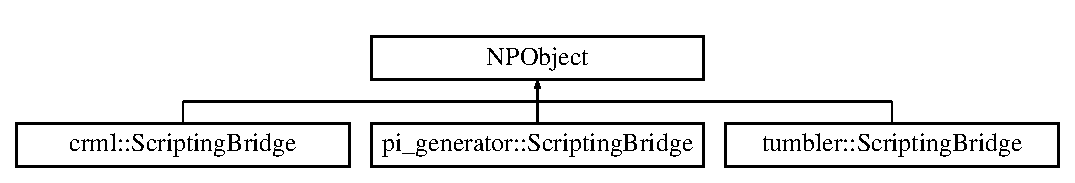
\includegraphics[height=2cm]{struct_n_p_object}
\end{center}
\end{figure}
\subsection*{Public Attributes}
\begin{DoxyCompactItemize}
\item 
\hyperlink{struct_n_p_class}{NPClass} $\ast$ \hyperlink{struct_n_p_object_a2c62da9b2fbf0399ee207289c326541b}{\_\-class}
\item 
uint32\_\-t \hyperlink{struct_n_p_object_a0f9e1d517ff19eebbdb732487a99bae2}{referenceCount}
\end{DoxyCompactItemize}


\subsection{Detailed Description}


Definition at line 325 of file npruntime.h.



\subsection{Member Data Documentation}
\hypertarget{struct_n_p_object_a2c62da9b2fbf0399ee207289c326541b}{
\index{NPObject@{NPObject}!\_\-class@{\_\-class}}
\index{\_\-class@{\_\-class}!NPObject@{NPObject}}
\subsubsection[{\_\-class}]{\setlength{\rightskip}{0pt plus 5cm}{\bf NPClass}$\ast$ {\bf NPObject::\_\-class}}}
\label{struct_n_p_object_a2c62da9b2fbf0399ee207289c326541b}


Definition at line 326 of file npruntime.h.

\hypertarget{struct_n_p_object_a0f9e1d517ff19eebbdb732487a99bae2}{
\index{NPObject@{NPObject}!referenceCount@{referenceCount}}
\index{referenceCount@{referenceCount}!NPObject@{NPObject}}
\subsubsection[{referenceCount}]{\setlength{\rightskip}{0pt plus 5cm}uint32\_\-t {\bf NPObject::referenceCount}}}
\label{struct_n_p_object_a0f9e1d517ff19eebbdb732487a99bae2}


Definition at line 327 of file npruntime.h.



The documentation for this struct was generated from the following file:\begin{DoxyCompactItemize}
\item 
/home/derek/dev/cell-\/grid-\/game/nacl/crml/crml/core/\hyperlink{npruntime_8h}{npruntime.h}\end{DoxyCompactItemize}

\hypertarget{classpi__generator_1_1_pi_generator}{
\section{pi\_\-generator::PiGenerator Class Reference}
\label{classpi__generator_1_1_pi_generator}\index{pi\_\-generator::PiGenerator@{pi\_\-generator::PiGenerator}}
}


{\ttfamily \#include $<$pi\_\-generator.h$>$}

\subsection*{Public Member Functions}
\begin{DoxyCompactItemize}
\item 
\hyperlink{classpi__generator_1_1_pi_generator_a0f5a55bbb942dee1b185447f0a7e24be}{PiGenerator} (\hyperlink{struct___n_p_p}{NPP} npp)
\item 
\hyperlink{classpi__generator_1_1_pi_generator_ac7d9c07492fd86678b8f66643e1e8c1e}{$\sim$PiGenerator} ()
\item 
NPObject $\ast$ \hyperlink{classpi__generator_1_1_pi_generator_ac65f31616ae3d223bdc01b91aea91762}{GetScriptableObject} ()
\item 
\hyperlink{npapi_8h_a56715bc92ac93f0447a05f852ce18828}{NPError} \hyperlink{classpi__generator_1_1_pi_generator_ad19c9de44971a5c08ee8e26a45598f38}{SetWindow} (\hyperlink{struct___n_p_window}{NPWindow} $\ast$window)
\item 
bool \hyperlink{classpi__generator_1_1_pi_generator_a47540afa1d21ef0b6e6ea7d986b71243}{Paint} ()
\item 
bool \hyperlink{classpi__generator_1_1_pi_generator_a02e8796485d878cbe8a42dcc2b204c4a}{quit} () const 
\item 
double \hyperlink{classpi__generator_1_1_pi_generator_a74119d27c1a01b50b91677f8089a0103}{pi} () const 
\item 
void $\ast$ \hyperlink{classpi__generator_1_1_pi_generator_a3e4279bb7732861b21ab6d1dcfc27429}{pixels} () const 
\item 
int \hyperlink{classpi__generator_1_1_pi_generator_ae3b2d276f4cf6209d7653f6fc4437fc4}{width} () const 
\item 
int \hyperlink{classpi__generator_1_1_pi_generator_a7cdc6f6c02a01a63e813c8357e901fb9}{height} () const 
\end{DoxyCompactItemize}


\subsection{Detailed Description}


Definition at line 22 of file pi\_\-generator.h.



\subsection{Constructor \& Destructor Documentation}
\hypertarget{classpi__generator_1_1_pi_generator_a0f5a55bbb942dee1b185447f0a7e24be}{
\index{pi\_\-generator::PiGenerator@{pi\_\-generator::PiGenerator}!PiGenerator@{PiGenerator}}
\index{PiGenerator@{PiGenerator}!pi_generator::PiGenerator@{pi\_\-generator::PiGenerator}}
\subsubsection[{PiGenerator}]{\setlength{\rightskip}{0pt plus 5cm}pi\_\-generator::PiGenerator::PiGenerator ({\bf NPP} {\em npp})\hspace{0.3cm}{\ttfamily  \mbox{[}explicit\mbox{]}}}}
\label{classpi__generator_1_1_pi_generator_a0f5a55bbb942dee1b185447f0a7e24be}


Definition at line 32 of file pi\_\-generator.cc.

\hypertarget{classpi__generator_1_1_pi_generator_ac7d9c07492fd86678b8f66643e1e8c1e}{
\index{pi\_\-generator::PiGenerator@{pi\_\-generator::PiGenerator}!$\sim$PiGenerator@{$\sim$PiGenerator}}
\index{$\sim$PiGenerator@{$\sim$PiGenerator}!pi_generator::PiGenerator@{pi\_\-generator::PiGenerator}}
\subsubsection[{$\sim$PiGenerator}]{\setlength{\rightskip}{0pt plus 5cm}pi\_\-generator::PiGenerator::$\sim$PiGenerator ()}}
\label{classpi__generator_1_1_pi_generator_ac7d9c07492fd86678b8f66643e1e8c1e}


Definition at line 43 of file pi\_\-generator.cc.



\subsection{Member Function Documentation}
\hypertarget{classpi__generator_1_1_pi_generator_ac65f31616ae3d223bdc01b91aea91762}{
\index{pi\_\-generator::PiGenerator@{pi\_\-generator::PiGenerator}!GetScriptableObject@{GetScriptableObject}}
\index{GetScriptableObject@{GetScriptableObject}!pi_generator::PiGenerator@{pi\_\-generator::PiGenerator}}
\subsubsection[{GetScriptableObject}]{\setlength{\rightskip}{0pt plus 5cm}NPObject $\ast$ pi\_\-generator::PiGenerator::GetScriptableObject ()}}
\label{classpi__generator_1_1_pi_generator_ac65f31616ae3d223bdc01b91aea91762}


Definition at line 54 of file pi\_\-generator.cc.

\hypertarget{classpi__generator_1_1_pi_generator_a7cdc6f6c02a01a63e813c8357e901fb9}{
\index{pi\_\-generator::PiGenerator@{pi\_\-generator::PiGenerator}!height@{height}}
\index{height@{height}!pi_generator::PiGenerator@{pi\_\-generator::PiGenerator}}
\subsubsection[{height}]{\setlength{\rightskip}{0pt plus 5cm}int pi\_\-generator::PiGenerator::height () const\hspace{0.3cm}{\ttfamily  \mbox{[}inline\mbox{]}}}}
\label{classpi__generator_1_1_pi_generator_a7cdc6f6c02a01a63e813c8357e901fb9}


Definition at line 42 of file pi\_\-generator.h.

\hypertarget{classpi__generator_1_1_pi_generator_a47540afa1d21ef0b6e6ea7d986b71243}{
\index{pi\_\-generator::PiGenerator@{pi\_\-generator::PiGenerator}!Paint@{Paint}}
\index{Paint@{Paint}!pi_generator::PiGenerator@{pi\_\-generator::PiGenerator}}
\subsubsection[{Paint}]{\setlength{\rightskip}{0pt plus 5cm}bool pi\_\-generator::PiGenerator::Paint ()}}
\label{classpi__generator_1_1_pi_generator_a47540afa1d21ef0b6e6ea7d986b71243}


Definition at line 78 of file pi\_\-generator.cc.

\hypertarget{classpi__generator_1_1_pi_generator_a74119d27c1a01b50b91677f8089a0103}{
\index{pi\_\-generator::PiGenerator@{pi\_\-generator::PiGenerator}!pi@{pi}}
\index{pi@{pi}!pi_generator::PiGenerator@{pi\_\-generator::PiGenerator}}
\subsubsection[{pi}]{\setlength{\rightskip}{0pt plus 5cm}double pi\_\-generator::PiGenerator::pi () const\hspace{0.3cm}{\ttfamily  \mbox{[}inline\mbox{]}}}}
\label{classpi__generator_1_1_pi_generator_a74119d27c1a01b50b91677f8089a0103}


Definition at line 33 of file pi\_\-generator.h.

\hypertarget{classpi__generator_1_1_pi_generator_a3e4279bb7732861b21ab6d1dcfc27429}{
\index{pi\_\-generator::PiGenerator@{pi\_\-generator::PiGenerator}!pixels@{pixels}}
\index{pixels@{pixels}!pi_generator::PiGenerator@{pi\_\-generator::PiGenerator}}
\subsubsection[{pixels}]{\setlength{\rightskip}{0pt plus 5cm}void$\ast$ pi\_\-generator::PiGenerator::pixels () const\hspace{0.3cm}{\ttfamily  \mbox{[}inline\mbox{]}}}}
\label{classpi__generator_1_1_pi_generator_a3e4279bb7732861b21ab6d1dcfc27429}


Definition at line 36 of file pi\_\-generator.h.

\hypertarget{classpi__generator_1_1_pi_generator_a02e8796485d878cbe8a42dcc2b204c4a}{
\index{pi\_\-generator::PiGenerator@{pi\_\-generator::PiGenerator}!quit@{quit}}
\index{quit@{quit}!pi_generator::PiGenerator@{pi\_\-generator::PiGenerator}}
\subsubsection[{quit}]{\setlength{\rightskip}{0pt plus 5cm}bool pi\_\-generator::PiGenerator::quit () const\hspace{0.3cm}{\ttfamily  \mbox{[}inline\mbox{]}}}}
\label{classpi__generator_1_1_pi_generator_a02e8796485d878cbe8a42dcc2b204c4a}


Definition at line 30 of file pi\_\-generator.h.

\hypertarget{classpi__generator_1_1_pi_generator_ad19c9de44971a5c08ee8e26a45598f38}{
\index{pi\_\-generator::PiGenerator@{pi\_\-generator::PiGenerator}!SetWindow@{SetWindow}}
\index{SetWindow@{SetWindow}!pi_generator::PiGenerator@{pi\_\-generator::PiGenerator}}
\subsubsection[{SetWindow}]{\setlength{\rightskip}{0pt plus 5cm}{\bf NPError} pi\_\-generator::PiGenerator::SetWindow ({\bf NPWindow} $\ast$ {\em window})}}
\label{classpi__generator_1_1_pi_generator_ad19c9de44971a5c08ee8e26a45598f38}


Definition at line 65 of file pi\_\-generator.cc.

\hypertarget{classpi__generator_1_1_pi_generator_ae3b2d276f4cf6209d7653f6fc4437fc4}{
\index{pi\_\-generator::PiGenerator@{pi\_\-generator::PiGenerator}!width@{width}}
\index{width@{width}!pi_generator::PiGenerator@{pi\_\-generator::PiGenerator}}
\subsubsection[{width}]{\setlength{\rightskip}{0pt plus 5cm}int pi\_\-generator::PiGenerator::width () const\hspace{0.3cm}{\ttfamily  \mbox{[}inline\mbox{]}}}}
\label{classpi__generator_1_1_pi_generator_ae3b2d276f4cf6209d7653f6fc4437fc4}


Definition at line 39 of file pi\_\-generator.h.



The documentation for this class was generated from the following files:\begin{DoxyCompactItemize}
\item 
/home/derek/dev/cell-\/grid-\/game/nacl/crml/crml/test/pi\_\-generator/\hyperlink{pi__generator_8h}{pi\_\-generator.h}\item 
/home/derek/dev/cell-\/grid-\/game/nacl/crml/crml/test/pi\_\-generator/\hyperlink{pi__generator_8cc}{pi\_\-generator.cc}\end{DoxyCompactItemize}

\hypertarget{class_plugin_object}{
\section{PluginObject Class Reference}
\label{class_plugin_object}\index{PluginObject@{PluginObject}}
}


{\ttfamily \#include $<$plugin\_\-object.h$>$}

\subsection*{Public Member Functions}
\begin{DoxyCompactItemize}
\item 
\hyperlink{class_plugin_object_ab24118f5b174beacb1b7f652bbbcf78d}{PluginObject} (\hyperlink{struct___n_p_p}{NPP} npp)
\item 
\hyperlink{class_plugin_object_ab2a72410c84a20133db4dec8ca92b277}{$\sim$PluginObject} ()
\item 
NPObject $\ast$ \hyperlink{class_plugin_object_ac551056ed0941b76c4161ba71e4cf449}{header} ()
\item 
\hyperlink{struct___n_p_p}{NPP} \hyperlink{class_plugin_object_a1a051ee92618bae8134b4d273d1d9982}{npp} () const 
\item 
void \hyperlink{class_plugin_object_a5e103c3aefcd2afb642c2414b92311ac}{New} (\hyperlink{npapi_8h_a6ab16d9f607aeb576061783638ae2973}{NPMIMEType} pluginType, int16\_\-t argc, char $\ast$argn\mbox{[}$\,$\mbox{]}, char $\ast$argv\mbox{[}$\,$\mbox{]})
\item 
void \hyperlink{class_plugin_object_a2a2774a67eadffc3f78d60e6c0559cf0}{SetWindow} (const \hyperlink{struct___n_p_window}{NPWindow} \&window)
\item 
bool \hyperlink{class_plugin_object_a4f594d05bd890649ca0f87ce30f03d26}{IsChecksumCheckSuccess} ()
\item 
std::string \hyperlink{class_plugin_object_a0ab936e960c08282554224a4570540aa}{ReportChecksum} ()
\item 
NPDevice $\ast$ \hyperlink{class_plugin_object_a0678b6675237f65d7679a400759b5c29}{GetDevice2D} ()
\item 
NPDeviceContext2D $\ast$ \hyperlink{class_plugin_object_ad121e4145b1f1cdcf878208919859e31}{GetContext2D} ()
\end{DoxyCompactItemize}
\subsection*{Static Public Member Functions}
\begin{DoxyCompactItemize}
\item 
static NPClass $\ast$ \hyperlink{class_plugin_object_a4b017230102036f1626af06df4864a95}{GetPluginClass} ()
\end{DoxyCompactItemize}
\subsection*{Protected Member Functions}
\begin{DoxyCompactItemize}
\item 
bool \hyperlink{class_plugin_object_add4437ed89953c9617ef7bd07ae32194}{InitializeCommandBuffer} ()
\item 
\hyperlink{class_plugin_object_ae85850715a04982f81d10136eca3b4f0}{PluginObject} (const \hyperlink{class_plugin_object}{PluginObject} \&)
\item 
void \hyperlink{class_plugin_object_a45243a3f962f41eb71fe0eeba7501262}{operator=} (const \hyperlink{class_plugin_object}{PluginObject} \&)
\end{DoxyCompactItemize}
\subsection*{Protected Attributes}
\begin{DoxyCompactItemize}
\item 
NPObject \hyperlink{class_plugin_object_a2d49cd1ca32c2522400d2505bd3e357e}{header\_\-}
\item 
\hyperlink{struct___n_p_p}{NPP} \hyperlink{class_plugin_object_a73abf33dbc703aaab8c133b4fc16a6f4}{npp\_\-}
\item 
NPObject $\ast$ \hyperlink{class_plugin_object_aa643ef173ea31331094fbf809d87b70d}{test\_\-object\_\-}
\item 
int \hyperlink{class_plugin_object_a60f6c920af50735f647d1715d7a27384}{dimensions\_\-}
\item 
NPDevice $\ast$ \hyperlink{class_plugin_object_a32c9649b557037cc8fbbf95f8c126c15}{device2d\_\-}
\item 
NPDevice $\ast$ \hyperlink{class_plugin_object_af2fd117655e58027408e3cde1f7283fb}{device3d\_\-}
\item 
PGLContext \hyperlink{class_plugin_object_a3819f8c68ea54fa3717c1487e288ee88}{pgl\_\-context\_\-}
\item 
NPDevice $\ast$ \hyperlink{class_plugin_object_aec43fcb4f77ce50598bb1851b100d045}{deviceaudio\_\-}
\item 
NPDeviceContextAudio \hyperlink{class_plugin_object_a29a7c72b105825ff135a29c9af9206f2}{context\_\-audio\_\-}
\item 
NPDeviceContext2D $\ast$ \hyperlink{class_plugin_object_ac4e47e096e7046c00152e0979a120059}{context2d\_\-}
\item 
unsigned int \hyperlink{class_plugin_object_ac792c1966624836cbbadf26eaeae4e52}{device2d\_\-checksum\_\-}
\item 
unsigned int \hyperlink{class_plugin_object_a1efe762777df7a3fc4b879d723598ef7}{plugin2d\_\-checksum\_\-}
\item 
int \hyperlink{class_plugin_object_a2aa3a91e29c0c89a9c887aaba1f1b9d0}{width\_\-}
\item 
int \hyperlink{class_plugin_object_af5872be14fbb29cf6cdf6df495766dd1}{height\_\-}
\end{DoxyCompactItemize}


\subsection{Detailed Description}


Definition at line 38 of file plugin\_\-object.h.



\subsection{Constructor \& Destructor Documentation}
\hypertarget{class_plugin_object_ab24118f5b174beacb1b7f652bbbcf78d}{
\index{PluginObject@{PluginObject}!PluginObject@{PluginObject}}
\index{PluginObject@{PluginObject}!PluginObject@{PluginObject}}
\subsubsection[{PluginObject}]{\setlength{\rightskip}{0pt plus 5cm}PluginObject::PluginObject ({\bf NPP} {\em npp})\hspace{0.3cm}{\ttfamily  \mbox{[}explicit\mbox{]}}}}
\label{class_plugin_object_ab24118f5b174beacb1b7f652bbbcf78d}


Definition at line 432 of file plugin\_\-object.cc.

\hypertarget{class_plugin_object_ab2a72410c84a20133db4dec8ca92b277}{
\index{PluginObject@{PluginObject}!$\sim$PluginObject@{$\sim$PluginObject}}
\index{$\sim$PluginObject@{$\sim$PluginObject}!PluginObject@{PluginObject}}
\subsubsection[{$\sim$PluginObject}]{\setlength{\rightskip}{0pt plus 5cm}PluginObject::$\sim$PluginObject ()}}
\label{class_plugin_object_ab2a72410c84a20133db4dec8ca92b277}


Definition at line 442 of file plugin\_\-object.cc.

\hypertarget{class_plugin_object_ae85850715a04982f81d10136eca3b4f0}{
\index{PluginObject@{PluginObject}!PluginObject@{PluginObject}}
\index{PluginObject@{PluginObject}!PluginObject@{PluginObject}}
\subsubsection[{PluginObject}]{\setlength{\rightskip}{0pt plus 5cm}PluginObject::PluginObject (const {\bf PluginObject} \&)\hspace{0.3cm}{\ttfamily  \mbox{[}protected\mbox{]}}}}
\label{class_plugin_object_ae85850715a04982f81d10136eca3b4f0}


\subsection{Member Function Documentation}
\hypertarget{class_plugin_object_ad121e4145b1f1cdcf878208919859e31}{
\index{PluginObject@{PluginObject}!GetContext2D@{GetContext2D}}
\index{GetContext2D@{GetContext2D}!PluginObject@{PluginObject}}
\subsubsection[{GetContext2D}]{\setlength{\rightskip}{0pt plus 5cm}NPDeviceContext2D $\ast$ PluginObject::GetContext2D ()}}
\label{class_plugin_object_ad121e4145b1f1cdcf878208919859e31}


Definition at line 502 of file plugin\_\-object.cc.

\hypertarget{class_plugin_object_a0678b6675237f65d7679a400759b5c29}{
\index{PluginObject@{PluginObject}!GetDevice2D@{GetDevice2D}}
\index{GetDevice2D@{GetDevice2D}!PluginObject@{PluginObject}}
\subsubsection[{GetDevice2D}]{\setlength{\rightskip}{0pt plus 5cm}NPDevice $\ast$ PluginObject::GetDevice2D ()}}
\label{class_plugin_object_a0678b6675237f65d7679a400759b5c29}


Definition at line 564 of file plugin\_\-object.cc.

\hypertarget{class_plugin_object_a4b017230102036f1626af06df4864a95}{
\index{PluginObject@{PluginObject}!GetPluginClass@{GetPluginClass}}
\index{GetPluginClass@{GetPluginClass}!PluginObject@{PluginObject}}
\subsubsection[{GetPluginClass}]{\setlength{\rightskip}{0pt plus 5cm}NPClass $\ast$ PluginObject::GetPluginClass ()\hspace{0.3cm}{\ttfamily  \mbox{[}static\mbox{]}}}}
\label{class_plugin_object_a4b017230102036f1626af06df4864a95}


Definition at line 450 of file plugin\_\-object.cc.

\hypertarget{class_plugin_object_ac551056ed0941b76c4161ba71e4cf449}{
\index{PluginObject@{PluginObject}!header@{header}}
\index{header@{header}!PluginObject@{PluginObject}}
\subsubsection[{header}]{\setlength{\rightskip}{0pt plus 5cm}NPObject$\ast$ PluginObject::header ()\hspace{0.3cm}{\ttfamily  \mbox{[}inline\mbox{]}}}}
\label{class_plugin_object_ac551056ed0941b76c4161ba71e4cf449}


Definition at line 45 of file plugin\_\-object.h.

\hypertarget{class_plugin_object_add4437ed89953c9617ef7bd07ae32194}{
\index{PluginObject@{PluginObject}!InitializeCommandBuffer@{InitializeCommandBuffer}}
\index{InitializeCommandBuffer@{InitializeCommandBuffer}!PluginObject@{PluginObject}}
\subsubsection[{InitializeCommandBuffer}]{\setlength{\rightskip}{0pt plus 5cm}bool PluginObject::InitializeCommandBuffer ()\hspace{0.3cm}{\ttfamily  \mbox{[}protected\mbox{]}}}}
\label{class_plugin_object_add4437ed89953c9617ef7bd07ae32194}
\hypertarget{class_plugin_object_a4f594d05bd890649ca0f87ce30f03d26}{
\index{PluginObject@{PluginObject}!IsChecksumCheckSuccess@{IsChecksumCheckSuccess}}
\index{IsChecksumCheckSuccess@{IsChecksumCheckSuccess}!PluginObject@{PluginObject}}
\subsubsection[{IsChecksumCheckSuccess}]{\setlength{\rightskip}{0pt plus 5cm}bool PluginObject::IsChecksumCheckSuccess ()}}
\label{class_plugin_object_a4f594d05bd890649ca0f87ce30f03d26}


Definition at line 569 of file plugin\_\-object.cc.

\hypertarget{class_plugin_object_a5e103c3aefcd2afb642c2414b92311ac}{
\index{PluginObject@{PluginObject}!New@{New}}
\index{New@{New}!PluginObject@{PluginObject}}
\subsubsection[{New}]{\setlength{\rightskip}{0pt plus 5cm}void PluginObject::New ({\bf NPMIMEType} {\em pluginType}, \/  int16\_\-t {\em argc}, \/  char $\ast$ {\em argn}\mbox{[}$\,$\mbox{]}, \/  char $\ast$ {\em argv}\mbox{[}$\,$\mbox{]})}}
\label{class_plugin_object_a5e103c3aefcd2afb642c2414b92311ac}


Definition at line 464 of file plugin\_\-object.cc.

\hypertarget{class_plugin_object_a1a051ee92618bae8134b4d273d1d9982}{
\index{PluginObject@{PluginObject}!npp@{npp}}
\index{npp@{npp}!PluginObject@{PluginObject}}
\subsubsection[{npp}]{\setlength{\rightskip}{0pt plus 5cm}{\bf NPP} PluginObject::npp () const\hspace{0.3cm}{\ttfamily  \mbox{[}inline\mbox{]}}}}
\label{class_plugin_object_a1a051ee92618bae8134b4d273d1d9982}


Definition at line 46 of file plugin\_\-object.h.

\hypertarget{class_plugin_object_a45243a3f962f41eb71fe0eeba7501262}{
\index{PluginObject@{PluginObject}!operator=@{operator=}}
\index{operator=@{operator=}!PluginObject@{PluginObject}}
\subsubsection[{operator=}]{\setlength{\rightskip}{0pt plus 5cm}void PluginObject::operator= (const {\bf PluginObject} \&)\hspace{0.3cm}{\ttfamily  \mbox{[}protected\mbox{]}}}}
\label{class_plugin_object_a45243a3f962f41eb71fe0eeba7501262}
\hypertarget{class_plugin_object_a0ab936e960c08282554224a4570540aa}{
\index{PluginObject@{PluginObject}!ReportChecksum@{ReportChecksum}}
\index{ReportChecksum@{ReportChecksum}!PluginObject@{PluginObject}}
\subsubsection[{ReportChecksum}]{\setlength{\rightskip}{0pt plus 5cm}std::string PluginObject::ReportChecksum ()}}
\label{class_plugin_object_a0ab936e960c08282554224a4570540aa}


Definition at line 576 of file plugin\_\-object.cc.

\hypertarget{class_plugin_object_a2a2774a67eadffc3f78d60e6c0559cf0}{
\index{PluginObject@{PluginObject}!SetWindow@{SetWindow}}
\index{SetWindow@{SetWindow}!PluginObject@{PluginObject}}
\subsubsection[{SetWindow}]{\setlength{\rightskip}{0pt plus 5cm}void PluginObject::SetWindow (const {\bf NPWindow} \& {\em window})}}
\label{class_plugin_object_a2a2774a67eadffc3f78d60e6c0559cf0}


Definition at line 507 of file plugin\_\-object.cc.



\subsection{Member Data Documentation}
\hypertarget{class_plugin_object_ac4e47e096e7046c00152e0979a120059}{
\index{PluginObject@{PluginObject}!context2d\_\-@{context2d\_\-}}
\index{context2d\_\-@{context2d\_\-}!PluginObject@{PluginObject}}
\subsubsection[{context2d\_\-}]{\setlength{\rightskip}{0pt plus 5cm}NPDeviceContext2D$\ast$ {\bf PluginObject::context2d\_\-}\hspace{0.3cm}{\ttfamily  \mbox{[}protected\mbox{]}}}}
\label{class_plugin_object_ac4e47e096e7046c00152e0979a120059}


Definition at line 74 of file plugin\_\-object.h.

\hypertarget{class_plugin_object_a29a7c72b105825ff135a29c9af9206f2}{
\index{PluginObject@{PluginObject}!context\_\-audio\_\-@{context\_\-audio\_\-}}
\index{context\_\-audio\_\-@{context\_\-audio\_\-}!PluginObject@{PluginObject}}
\subsubsection[{context\_\-audio\_\-}]{\setlength{\rightskip}{0pt plus 5cm}NPDeviceContextAudio {\bf PluginObject::context\_\-audio\_\-}\hspace{0.3cm}{\ttfamily  \mbox{[}protected\mbox{]}}}}
\label{class_plugin_object_a29a7c72b105825ff135a29c9af9206f2}


Definition at line 72 of file plugin\_\-object.h.

\hypertarget{class_plugin_object_a32c9649b557037cc8fbbf95f8c126c15}{
\index{PluginObject@{PluginObject}!device2d\_\-@{device2d\_\-}}
\index{device2d\_\-@{device2d\_\-}!PluginObject@{PluginObject}}
\subsubsection[{device2d\_\-}]{\setlength{\rightskip}{0pt plus 5cm}NPDevice$\ast$ {\bf PluginObject::device2d\_\-}\hspace{0.3cm}{\ttfamily  \mbox{[}protected\mbox{]}}}}
\label{class_plugin_object_a32c9649b557037cc8fbbf95f8c126c15}


Definition at line 64 of file plugin\_\-object.h.

\hypertarget{class_plugin_object_ac792c1966624836cbbadf26eaeae4e52}{
\index{PluginObject@{PluginObject}!device2d\_\-checksum\_\-@{device2d\_\-checksum\_\-}}
\index{device2d\_\-checksum\_\-@{device2d\_\-checksum\_\-}!PluginObject@{PluginObject}}
\subsubsection[{device2d\_\-checksum\_\-}]{\setlength{\rightskip}{0pt plus 5cm}unsigned int {\bf PluginObject::device2d\_\-checksum\_\-}\hspace{0.3cm}{\ttfamily  \mbox{[}protected\mbox{]}}}}
\label{class_plugin_object_ac792c1966624836cbbadf26eaeae4e52}


Definition at line 76 of file plugin\_\-object.h.

\hypertarget{class_plugin_object_af2fd117655e58027408e3cde1f7283fb}{
\index{PluginObject@{PluginObject}!device3d\_\-@{device3d\_\-}}
\index{device3d\_\-@{device3d\_\-}!PluginObject@{PluginObject}}
\subsubsection[{device3d\_\-}]{\setlength{\rightskip}{0pt plus 5cm}NPDevice$\ast$ {\bf PluginObject::device3d\_\-}\hspace{0.3cm}{\ttfamily  \mbox{[}protected\mbox{]}}}}
\label{class_plugin_object_af2fd117655e58027408e3cde1f7283fb}


Definition at line 65 of file plugin\_\-object.h.

\hypertarget{class_plugin_object_aec43fcb4f77ce50598bb1851b100d045}{
\index{PluginObject@{PluginObject}!deviceaudio\_\-@{deviceaudio\_\-}}
\index{deviceaudio\_\-@{deviceaudio\_\-}!PluginObject@{PluginObject}}
\subsubsection[{deviceaudio\_\-}]{\setlength{\rightskip}{0pt plus 5cm}NPDevice$\ast$ {\bf PluginObject::deviceaudio\_\-}\hspace{0.3cm}{\ttfamily  \mbox{[}protected\mbox{]}}}}
\label{class_plugin_object_aec43fcb4f77ce50598bb1851b100d045}


Definition at line 69 of file plugin\_\-object.h.

\hypertarget{class_plugin_object_a60f6c920af50735f647d1715d7a27384}{
\index{PluginObject@{PluginObject}!dimensions\_\-@{dimensions\_\-}}
\index{dimensions\_\-@{dimensions\_\-}!PluginObject@{PluginObject}}
\subsubsection[{dimensions\_\-}]{\setlength{\rightskip}{0pt plus 5cm}int {\bf PluginObject::dimensions\_\-}\hspace{0.3cm}{\ttfamily  \mbox{[}protected\mbox{]}}}}
\label{class_plugin_object_a60f6c920af50735f647d1715d7a27384}


Definition at line 62 of file plugin\_\-object.h.

\hypertarget{class_plugin_object_a2d49cd1ca32c2522400d2505bd3e357e}{
\index{PluginObject@{PluginObject}!header\_\-@{header\_\-}}
\index{header\_\-@{header\_\-}!PluginObject@{PluginObject}}
\subsubsection[{header\_\-}]{\setlength{\rightskip}{0pt plus 5cm}NPObject {\bf PluginObject::header\_\-}\hspace{0.3cm}{\ttfamily  \mbox{[}protected\mbox{]}}}}
\label{class_plugin_object_a2d49cd1ca32c2522400d2505bd3e357e}


Definition at line 59 of file plugin\_\-object.h.

\hypertarget{class_plugin_object_af5872be14fbb29cf6cdf6df495766dd1}{
\index{PluginObject@{PluginObject}!height\_\-@{height\_\-}}
\index{height\_\-@{height\_\-}!PluginObject@{PluginObject}}
\subsubsection[{height\_\-}]{\setlength{\rightskip}{0pt plus 5cm}int {\bf PluginObject::height\_\-}\hspace{0.3cm}{\ttfamily  \mbox{[}protected\mbox{]}}}}
\label{class_plugin_object_af5872be14fbb29cf6cdf6df495766dd1}


Definition at line 80 of file plugin\_\-object.h.

\hypertarget{class_plugin_object_a73abf33dbc703aaab8c133b4fc16a6f4}{
\index{PluginObject@{PluginObject}!npp\_\-@{npp\_\-}}
\index{npp\_\-@{npp\_\-}!PluginObject@{PluginObject}}
\subsubsection[{npp\_\-}]{\setlength{\rightskip}{0pt plus 5cm}{\bf NPP} {\bf PluginObject::npp\_\-}\hspace{0.3cm}{\ttfamily  \mbox{[}protected\mbox{]}}}}
\label{class_plugin_object_a73abf33dbc703aaab8c133b4fc16a6f4}


Definition at line 60 of file plugin\_\-object.h.

\hypertarget{class_plugin_object_a3819f8c68ea54fa3717c1487e288ee88}{
\index{PluginObject@{PluginObject}!pgl\_\-context\_\-@{pgl\_\-context\_\-}}
\index{pgl\_\-context\_\-@{pgl\_\-context\_\-}!PluginObject@{PluginObject}}
\subsubsection[{pgl\_\-context\_\-}]{\setlength{\rightskip}{0pt plus 5cm}PGLContext {\bf PluginObject::pgl\_\-context\_\-}\hspace{0.3cm}{\ttfamily  \mbox{[}protected\mbox{]}}}}
\label{class_plugin_object_a3819f8c68ea54fa3717c1487e288ee88}


Definition at line 67 of file plugin\_\-object.h.

\hypertarget{class_plugin_object_a1efe762777df7a3fc4b879d723598ef7}{
\index{PluginObject@{PluginObject}!plugin2d\_\-checksum\_\-@{plugin2d\_\-checksum\_\-}}
\index{plugin2d\_\-checksum\_\-@{plugin2d\_\-checksum\_\-}!PluginObject@{PluginObject}}
\subsubsection[{plugin2d\_\-checksum\_\-}]{\setlength{\rightskip}{0pt plus 5cm}unsigned int {\bf PluginObject::plugin2d\_\-checksum\_\-}\hspace{0.3cm}{\ttfamily  \mbox{[}protected\mbox{]}}}}
\label{class_plugin_object_a1efe762777df7a3fc4b879d723598ef7}


Definition at line 77 of file plugin\_\-object.h.

\hypertarget{class_plugin_object_aa643ef173ea31331094fbf809d87b70d}{
\index{PluginObject@{PluginObject}!test\_\-object\_\-@{test\_\-object\_\-}}
\index{test\_\-object\_\-@{test\_\-object\_\-}!PluginObject@{PluginObject}}
\subsubsection[{test\_\-object\_\-}]{\setlength{\rightskip}{0pt plus 5cm}NPObject$\ast$ {\bf PluginObject::test\_\-object\_\-}\hspace{0.3cm}{\ttfamily  \mbox{[}protected\mbox{]}}}}
\label{class_plugin_object_aa643ef173ea31331094fbf809d87b70d}


Definition at line 61 of file plugin\_\-object.h.

\hypertarget{class_plugin_object_a2aa3a91e29c0c89a9c887aaba1f1b9d0}{
\index{PluginObject@{PluginObject}!width\_\-@{width\_\-}}
\index{width\_\-@{width\_\-}!PluginObject@{PluginObject}}
\subsubsection[{width\_\-}]{\setlength{\rightskip}{0pt plus 5cm}int {\bf PluginObject::width\_\-}\hspace{0.3cm}{\ttfamily  \mbox{[}protected\mbox{]}}}}
\label{class_plugin_object_a2aa3a91e29c0c89a9c887aaba1f1b9d0}


Definition at line 79 of file plugin\_\-object.h.



The documentation for this class was generated from the following files:\begin{DoxyCompactItemize}
\item 
/home/derek/dev/cell-\/grid-\/game/nacl/crml/crml/core/\hyperlink{plugin__object_8h}{plugin\_\-object.h}\item 
/home/derek/dev/cell-\/grid-\/game/nacl/crml/crml/core/\hyperlink{plugin__object_8cc}{plugin\_\-object.cc}\end{DoxyCompactItemize}

\hypertarget{classhttpd_1_1_quittable_h_t_t_p_handler}{
\section{httpd::QuittableHTTPHandler Class Reference}
\label{classhttpd_1_1_quittable_h_t_t_p_handler}\index{httpd::QuittableHTTPHandler@{httpd::QuittableHTTPHandler}}
}
\subsection*{Public Member Functions}
\begin{DoxyCompactItemize}
\item 
def \hyperlink{classhttpd_1_1_quittable_h_t_t_p_handler_addc36268dbff72748204a5baae7a6e5b}{do\_\-GET}
\item 
def \hyperlink{classhttpd_1_1_quittable_h_t_t_p_handler_addc36268dbff72748204a5baae7a6e5b}{do\_\-GET}
\end{DoxyCompactItemize}


\subsection{Detailed Description}


Definition at line 73 of file httpd.py.



\subsection{Member Function Documentation}
\hypertarget{classhttpd_1_1_quittable_h_t_t_p_handler_addc36268dbff72748204a5baae7a6e5b}{
\index{httpd::QuittableHTTPHandler@{httpd::QuittableHTTPHandler}!do\_\-GET@{do\_\-GET}}
\index{do\_\-GET@{do\_\-GET}!httpd::QuittableHTTPHandler@{httpd::QuittableHTTPHandler}}
\subsubsection[{do\_\-GET}]{\setlength{\rightskip}{0pt plus 5cm}def httpd::QuittableHTTPHandler::do\_\-GET ( {\em self})}}
\label{classhttpd_1_1_quittable_h_t_t_p_handler_addc36268dbff72748204a5baae7a6e5b}


Definition at line 74 of file httpd.py.

\hypertarget{classhttpd_1_1_quittable_h_t_t_p_handler_addc36268dbff72748204a5baae7a6e5b}{
\index{httpd::QuittableHTTPHandler@{httpd::QuittableHTTPHandler}!do\_\-GET@{do\_\-GET}}
\index{do\_\-GET@{do\_\-GET}!httpd::QuittableHTTPHandler@{httpd::QuittableHTTPHandler}}
\subsubsection[{do\_\-GET}]{\setlength{\rightskip}{0pt plus 5cm}def httpd::QuittableHTTPHandler::do\_\-GET ( {\em self})}}
\label{classhttpd_1_1_quittable_h_t_t_p_handler_addc36268dbff72748204a5baae7a6e5b}


Definition at line 74 of file httpd.py.



The documentation for this class was generated from the following files:\begin{DoxyCompactItemize}
\item 
/home/derek/dev/crml/crml/src/web/\hyperlink{src_2web_2httpd_8py}{httpd.py}\item 
/home/derek/dev/crml/crml/test/\hyperlink{test_2httpd_8py}{httpd.py}\end{DoxyCompactItemize}

\hypertarget{classhttpd_1_1_quittable_h_t_t_p_server}{
\section{httpd::QuittableHTTPServer Class Reference}
\label{classhttpd_1_1_quittable_h_t_t_p_server}\index{httpd::QuittableHTTPServer@{httpd::QuittableHTTPServer}}
}
\subsection*{Public Member Functions}
\begin{DoxyCompactItemize}
\item 
def \hyperlink{classhttpd_1_1_quittable_h_t_t_p_server_ad7da0003b17805e7e629fa09a3a8f187}{serve\_\-forever}
\item 
def \hyperlink{classhttpd_1_1_quittable_h_t_t_p_server_a7d527531f10ecbcb1db670cf816bbcbd}{shutdown}
\end{DoxyCompactItemize}
\subsection*{Public Attributes}
\begin{DoxyCompactItemize}
\item 
\hyperlink{classhttpd_1_1_quittable_h_t_t_p_server_a72e565dcba798dfd43d18268e92075a8}{is\_\-running}
\end{DoxyCompactItemize}


\subsection{Detailed Description}


Definition at line 50 of file httpd.py.



\subsection{Member Function Documentation}
\hypertarget{classhttpd_1_1_quittable_h_t_t_p_server_ad7da0003b17805e7e629fa09a3a8f187}{
\index{httpd::QuittableHTTPServer@{httpd::QuittableHTTPServer}!serve\_\-forever@{serve\_\-forever}}
\index{serve\_\-forever@{serve\_\-forever}!httpd::QuittableHTTPServer@{httpd::QuittableHTTPServer}}
\subsubsection[{serve\_\-forever}]{\setlength{\rightskip}{0pt plus 5cm}def httpd::QuittableHTTPServer::serve\_\-forever ( {\em self})}}
\label{classhttpd_1_1_quittable_h_t_t_p_server_ad7da0003b17805e7e629fa09a3a8f187}


Definition at line 51 of file httpd.py.

\hypertarget{classhttpd_1_1_quittable_h_t_t_p_server_a7d527531f10ecbcb1db670cf816bbcbd}{
\index{httpd::QuittableHTTPServer@{httpd::QuittableHTTPServer}!shutdown@{shutdown}}
\index{shutdown@{shutdown}!httpd::QuittableHTTPServer@{httpd::QuittableHTTPServer}}
\subsubsection[{shutdown}]{\setlength{\rightskip}{0pt plus 5cm}def httpd::QuittableHTTPServer::shutdown ( {\em self})}}
\label{classhttpd_1_1_quittable_h_t_t_p_server_a7d527531f10ecbcb1db670cf816bbcbd}


Definition at line 56 of file httpd.py.



\subsection{Member Data Documentation}
\hypertarget{classhttpd_1_1_quittable_h_t_t_p_server_a72e565dcba798dfd43d18268e92075a8}{
\index{httpd::QuittableHTTPServer@{httpd::QuittableHTTPServer}!is\_\-running@{is\_\-running}}
\index{is\_\-running@{is\_\-running}!httpd::QuittableHTTPServer@{httpd::QuittableHTTPServer}}
\subsubsection[{is\_\-running}]{\setlength{\rightskip}{0pt plus 5cm}{\bf httpd::QuittableHTTPServer::is\_\-running}}}
\label{classhttpd_1_1_quittable_h_t_t_p_server_a72e565dcba798dfd43d18268e92075a8}


Definition at line 52 of file httpd.py.



The documentation for this class was generated from the following file:\begin{DoxyCompactItemize}
\item 
/home/derek/dev/cell-\/grid-\/game/nacl/crml/crml/web/\hyperlink{httpd_8py}{httpd.py}\end{DoxyCompactItemize}

\hypertarget{classcrml_1_1_scripting_bridge}{
\section{crml::ScriptingBridge Class Reference}
\label{classcrml_1_1_scripting_bridge}\index{crml::ScriptingBridge@{crml::ScriptingBridge}}
}


{\ttfamily \#include $<$scripting\_\-bridge.h$>$}

Inheritance diagram for crml::ScriptingBridge:\begin{figure}[H]
\begin{center}
\leavevmode
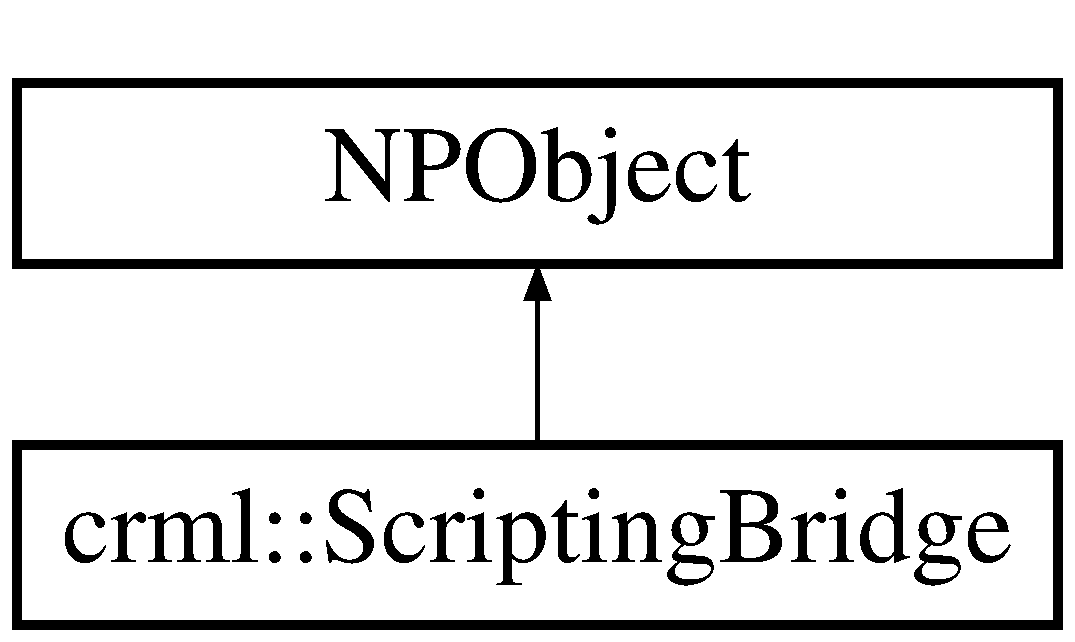
\includegraphics[height=2cm]{classcrml_1_1_scripting_bridge}
\end{center}
\end{figure}
\subsection*{Public Types}
\begin{DoxyCompactItemize}
\item 
typedef bool(ScriptingBridge::$\ast$ \hyperlink{classcrml_1_1_scripting_bridge_a914d759a85c8280e66b435b824c6f06e}{Method} )(const \hyperlink{struct___n_p_variant}{NPVariant} $\ast$args, uint32\_\-t arg\_\-count, \hyperlink{struct___n_p_variant}{NPVariant} $\ast$result)
\item 
typedef bool(ScriptingBridge::$\ast$ \hyperlink{classcrml_1_1_scripting_bridge_a784ee1ef915801e5c5facde3d6c70aef}{Property} )(\hyperlink{struct___n_p_variant}{NPVariant} $\ast$result)
\end{DoxyCompactItemize}
\subsection*{Public Member Functions}
\begin{DoxyCompactItemize}
\item 
\hyperlink{classcrml_1_1_scripting_bridge_acffa45f2fbbf75e2899dad0715694965}{ScriptingBridge} (\hyperlink{struct___n_p_p}{NPP} npp)
\item 
virtual \hyperlink{classcrml_1_1_scripting_bridge_a2762a9e0d5c5c4c4e43b7740a88b4964}{$\sim$ScriptingBridge} ()
\item 
void \hyperlink{classcrml_1_1_scripting_bridge_ad03efd11014ce3a9aeb0909d9d315f86}{Invalidate} ()
\item 
bool \hyperlink{classcrml_1_1_scripting_bridge_aa8546ab90cbe399399733a53495ec9b3}{HasMethod} (\hyperlink{npruntime_8h_a3ce51391e08bd3e24128c342b1d055b9}{NPIdentifier} name)
\item 
bool \hyperlink{classcrml_1_1_scripting_bridge_ac76ef418e8199808e99a562f678d670c}{Invoke} (\hyperlink{npruntime_8h_a3ce51391e08bd3e24128c342b1d055b9}{NPIdentifier} name, const \hyperlink{struct___n_p_variant}{NPVariant} $\ast$args, uint32\_\-t arg\_\-count, \hyperlink{struct___n_p_variant}{NPVariant} $\ast$result)
\item 
bool \hyperlink{classcrml_1_1_scripting_bridge_a3e96aad4ad401ace8b78213f68faf29b}{InvokeDefault} (const \hyperlink{struct___n_p_variant}{NPVariant} $\ast$args, uint32\_\-t arg\_\-count, \hyperlink{struct___n_p_variant}{NPVariant} $\ast$result)
\item 
bool \hyperlink{classcrml_1_1_scripting_bridge_a349e22860ef3ce03412e1914cccc12ba}{HasProperty} (\hyperlink{npruntime_8h_a3ce51391e08bd3e24128c342b1d055b9}{NPIdentifier} name)
\item 
bool \hyperlink{classcrml_1_1_scripting_bridge_a9e52acfa32559fa8dfa41cf2898a1ba6}{GetProperty} (\hyperlink{npruntime_8h_a3ce51391e08bd3e24128c342b1d055b9}{NPIdentifier} name, \hyperlink{struct___n_p_variant}{NPVariant} $\ast$result)
\item 
bool \hyperlink{classcrml_1_1_scripting_bridge_acbdfa02a2c2e6c6358fbaa825b725230}{SetProperty} (\hyperlink{npruntime_8h_a3ce51391e08bd3e24128c342b1d055b9}{NPIdentifier} name, const \hyperlink{struct___n_p_variant}{NPVariant} $\ast$value)
\item 
bool \hyperlink{classcrml_1_1_scripting_bridge_a406ed77fb660dc3879a71e3ebb59b0a4}{RemoveProperty} (\hyperlink{npruntime_8h_a3ce51391e08bd3e24128c342b1d055b9}{NPIdentifier} name)
\item 
bool \hyperlink{classcrml_1_1_scripting_bridge_a0de2960917327478a47eee5d7f780107}{Paint} (const \hyperlink{struct___n_p_variant}{NPVariant} $\ast$args, uint32\_\-t arg\_\-count, \hyperlink{struct___n_p_variant}{NPVariant} $\ast$result)
\end{DoxyCompactItemize}
\subsection*{Static Public Member Functions}
\begin{DoxyCompactItemize}
\item 
static bool \hyperlink{classcrml_1_1_scripting_bridge_a578877afcfdf32ca1330732bbf6739ad}{InitializeIdentifiers} ()
\end{DoxyCompactItemize}
\subsection*{Static Public Attributes}
\begin{DoxyCompactItemize}
\item 
static \hyperlink{struct_n_p_class}{NPClass} \hyperlink{classcrml_1_1_scripting_bridge_a1a005096b44959f11d3759a6c3540534}{np\_\-class}
\end{DoxyCompactItemize}


\subsection{Detailed Description}


Definition at line 12 of file scripting\_\-bridge.h.



\subsection{Member Typedef Documentation}
\hypertarget{classcrml_1_1_scripting_bridge_a914d759a85c8280e66b435b824c6f06e}{
\index{crml::ScriptingBridge@{crml::ScriptingBridge}!Method@{Method}}
\index{Method@{Method}!crml::ScriptingBridge@{crml::ScriptingBridge}}
\subsubsection[{Method}]{\setlength{\rightskip}{0pt plus 5cm}typedef bool(ScriptingBridge::$\ast$ {\bf crml::ScriptingBridge::Method})(const {\bf NPVariant} $\ast$args, uint32\_\-t arg\_\-count, {\bf NPVariant} $\ast$result)}}
\label{classcrml_1_1_scripting_bridge_a914d759a85c8280e66b435b824c6f06e}


Definition at line 14 of file scripting\_\-bridge.h.

\hypertarget{classcrml_1_1_scripting_bridge_a784ee1ef915801e5c5facde3d6c70aef}{
\index{crml::ScriptingBridge@{crml::ScriptingBridge}!Property@{Property}}
\index{Property@{Property}!crml::ScriptingBridge@{crml::ScriptingBridge}}
\subsubsection[{Property}]{\setlength{\rightskip}{0pt plus 5cm}typedef bool(ScriptingBridge::$\ast$ {\bf crml::ScriptingBridge::Property})({\bf NPVariant} $\ast$result)}}
\label{classcrml_1_1_scripting_bridge_a784ee1ef915801e5c5facde3d6c70aef}


Definition at line 17 of file scripting\_\-bridge.h.



\subsection{Constructor \& Destructor Documentation}
\hypertarget{classcrml_1_1_scripting_bridge_acffa45f2fbbf75e2899dad0715694965}{
\index{crml::ScriptingBridge@{crml::ScriptingBridge}!ScriptingBridge@{ScriptingBridge}}
\index{ScriptingBridge@{ScriptingBridge}!crml::ScriptingBridge@{crml::ScriptingBridge}}
\subsubsection[{ScriptingBridge}]{\setlength{\rightskip}{0pt plus 5cm}crml::ScriptingBridge::ScriptingBridge ({\bf NPP} {\em npp})\hspace{0.3cm}{\ttfamily  \mbox{[}inline, explicit\mbox{]}}}}
\label{classcrml_1_1_scripting_bridge_acffa45f2fbbf75e2899dad0715694965}


Definition at line 19 of file scripting\_\-bridge.h.

\hypertarget{classcrml_1_1_scripting_bridge_a2762a9e0d5c5c4c4e43b7740a88b4964}{
\index{crml::ScriptingBridge@{crml::ScriptingBridge}!$\sim$ScriptingBridge@{$\sim$ScriptingBridge}}
\index{$\sim$ScriptingBridge@{$\sim$ScriptingBridge}!crml::ScriptingBridge@{crml::ScriptingBridge}}
\subsubsection[{$\sim$ScriptingBridge}]{\setlength{\rightskip}{0pt plus 5cm}virtual crml::ScriptingBridge::$\sim$ScriptingBridge ()\hspace{0.3cm}{\ttfamily  \mbox{[}virtual\mbox{]}}}}
\label{classcrml_1_1_scripting_bridge_a2762a9e0d5c5c4c4e43b7740a88b4964}


\subsection{Member Function Documentation}
\hypertarget{classcrml_1_1_scripting_bridge_a9e52acfa32559fa8dfa41cf2898a1ba6}{
\index{crml::ScriptingBridge@{crml::ScriptingBridge}!GetProperty@{GetProperty}}
\index{GetProperty@{GetProperty}!crml::ScriptingBridge@{crml::ScriptingBridge}}
\subsubsection[{GetProperty}]{\setlength{\rightskip}{0pt plus 5cm}bool crml::ScriptingBridge::GetProperty ({\bf NPIdentifier} {\em name}, \/  {\bf NPVariant} $\ast$ {\em result})}}
\label{classcrml_1_1_scripting_bridge_a9e52acfa32559fa8dfa41cf2898a1ba6}
\hypertarget{classcrml_1_1_scripting_bridge_aa8546ab90cbe399399733a53495ec9b3}{
\index{crml::ScriptingBridge@{crml::ScriptingBridge}!HasMethod@{HasMethod}}
\index{HasMethod@{HasMethod}!crml::ScriptingBridge@{crml::ScriptingBridge}}
\subsubsection[{HasMethod}]{\setlength{\rightskip}{0pt plus 5cm}bool crml::ScriptingBridge::HasMethod ({\bf NPIdentifier} {\em name})}}
\label{classcrml_1_1_scripting_bridge_aa8546ab90cbe399399733a53495ec9b3}
\hypertarget{classcrml_1_1_scripting_bridge_a349e22860ef3ce03412e1914cccc12ba}{
\index{crml::ScriptingBridge@{crml::ScriptingBridge}!HasProperty@{HasProperty}}
\index{HasProperty@{HasProperty}!crml::ScriptingBridge@{crml::ScriptingBridge}}
\subsubsection[{HasProperty}]{\setlength{\rightskip}{0pt plus 5cm}bool crml::ScriptingBridge::HasProperty ({\bf NPIdentifier} {\em name})}}
\label{classcrml_1_1_scripting_bridge_a349e22860ef3ce03412e1914cccc12ba}
\hypertarget{classcrml_1_1_scripting_bridge_a578877afcfdf32ca1330732bbf6739ad}{
\index{crml::ScriptingBridge@{crml::ScriptingBridge}!InitializeIdentifiers@{InitializeIdentifiers}}
\index{InitializeIdentifiers@{InitializeIdentifiers}!crml::ScriptingBridge@{crml::ScriptingBridge}}
\subsubsection[{InitializeIdentifiers}]{\setlength{\rightskip}{0pt plus 5cm}static bool crml::ScriptingBridge::InitializeIdentifiers ()\hspace{0.3cm}{\ttfamily  \mbox{[}static\mbox{]}}}}
\label{classcrml_1_1_scripting_bridge_a578877afcfdf32ca1330732bbf6739ad}
\hypertarget{classcrml_1_1_scripting_bridge_ad03efd11014ce3a9aeb0909d9d315f86}{
\index{crml::ScriptingBridge@{crml::ScriptingBridge}!Invalidate@{Invalidate}}
\index{Invalidate@{Invalidate}!crml::ScriptingBridge@{crml::ScriptingBridge}}
\subsubsection[{Invalidate}]{\setlength{\rightskip}{0pt plus 5cm}void crml::ScriptingBridge::Invalidate ()}}
\label{classcrml_1_1_scripting_bridge_ad03efd11014ce3a9aeb0909d9d315f86}
\hypertarget{classcrml_1_1_scripting_bridge_ac76ef418e8199808e99a562f678d670c}{
\index{crml::ScriptingBridge@{crml::ScriptingBridge}!Invoke@{Invoke}}
\index{Invoke@{Invoke}!crml::ScriptingBridge@{crml::ScriptingBridge}}
\subsubsection[{Invoke}]{\setlength{\rightskip}{0pt plus 5cm}bool crml::ScriptingBridge::Invoke ({\bf NPIdentifier} {\em name}, \/  const {\bf NPVariant} $\ast$ {\em args}, \/  uint32\_\-t {\em arg\_\-count}, \/  {\bf NPVariant} $\ast$ {\em result})}}
\label{classcrml_1_1_scripting_bridge_ac76ef418e8199808e99a562f678d670c}
\hypertarget{classcrml_1_1_scripting_bridge_a3e96aad4ad401ace8b78213f68faf29b}{
\index{crml::ScriptingBridge@{crml::ScriptingBridge}!InvokeDefault@{InvokeDefault}}
\index{InvokeDefault@{InvokeDefault}!crml::ScriptingBridge@{crml::ScriptingBridge}}
\subsubsection[{InvokeDefault}]{\setlength{\rightskip}{0pt plus 5cm}bool crml::ScriptingBridge::InvokeDefault (const {\bf NPVariant} $\ast$ {\em args}, \/  uint32\_\-t {\em arg\_\-count}, \/  {\bf NPVariant} $\ast$ {\em result})}}
\label{classcrml_1_1_scripting_bridge_a3e96aad4ad401ace8b78213f68faf29b}
\hypertarget{classcrml_1_1_scripting_bridge_a0de2960917327478a47eee5d7f780107}{
\index{crml::ScriptingBridge@{crml::ScriptingBridge}!Paint@{Paint}}
\index{Paint@{Paint}!crml::ScriptingBridge@{crml::ScriptingBridge}}
\subsubsection[{Paint}]{\setlength{\rightskip}{0pt plus 5cm}bool crml::ScriptingBridge::Paint (const {\bf NPVariant} $\ast$ {\em args}, \/  uint32\_\-t {\em arg\_\-count}, \/  {\bf NPVariant} $\ast$ {\em result})}}
\label{classcrml_1_1_scripting_bridge_a0de2960917327478a47eee5d7f780107}
\hypertarget{classcrml_1_1_scripting_bridge_a406ed77fb660dc3879a71e3ebb59b0a4}{
\index{crml::ScriptingBridge@{crml::ScriptingBridge}!RemoveProperty@{RemoveProperty}}
\index{RemoveProperty@{RemoveProperty}!crml::ScriptingBridge@{crml::ScriptingBridge}}
\subsubsection[{RemoveProperty}]{\setlength{\rightskip}{0pt plus 5cm}bool crml::ScriptingBridge::RemoveProperty ({\bf NPIdentifier} {\em name})}}
\label{classcrml_1_1_scripting_bridge_a406ed77fb660dc3879a71e3ebb59b0a4}
\hypertarget{classcrml_1_1_scripting_bridge_acbdfa02a2c2e6c6358fbaa825b725230}{
\index{crml::ScriptingBridge@{crml::ScriptingBridge}!SetProperty@{SetProperty}}
\index{SetProperty@{SetProperty}!crml::ScriptingBridge@{crml::ScriptingBridge}}
\subsubsection[{SetProperty}]{\setlength{\rightskip}{0pt plus 5cm}bool crml::ScriptingBridge::SetProperty ({\bf NPIdentifier} {\em name}, \/  const {\bf NPVariant} $\ast$ {\em value})}}
\label{classcrml_1_1_scripting_bridge_acbdfa02a2c2e6c6358fbaa825b725230}


\subsection{Member Data Documentation}
\hypertarget{classcrml_1_1_scripting_bridge_a1a005096b44959f11d3759a6c3540534}{
\index{crml::ScriptingBridge@{crml::ScriptingBridge}!np\_\-class@{np\_\-class}}
\index{np\_\-class@{np\_\-class}!crml::ScriptingBridge@{crml::ScriptingBridge}}
\subsubsection[{np\_\-class}]{\setlength{\rightskip}{0pt plus 5cm}{\bf NPClass} {\bf crml::ScriptingBridge::np\_\-class}\hspace{0.3cm}{\ttfamily  \mbox{[}static\mbox{]}}}}
\label{classcrml_1_1_scripting_bridge_a1a005096b44959f11d3759a6c3540534}


Definition at line 40 of file scripting\_\-bridge.h.



The documentation for this class was generated from the following file:\begin{DoxyCompactItemize}
\item 
/home/derek/dev/cell-\/grid-\/game/nacl/crml/crml/core/\hyperlink{core_2scripting__bridge_8h}{scripting\_\-bridge.h}\end{DoxyCompactItemize}

\hypertarget{classtumbler_1_1_scripting_bridge}{
\section{tumbler::ScriptingBridge Class Reference}
\label{classtumbler_1_1_scripting_bridge}\index{tumbler::ScriptingBridge@{tumbler::ScriptingBridge}}
}


{\ttfamily \#include $<$scripting\_\-bridge.h$>$}

\subsection*{Public Types}
\begin{DoxyCompactItemize}
\item 
typedef bool(ScriptingBridge::$\ast$ \hyperlink{classtumbler_1_1_scripting_bridge_addb1badb0e891b38c6d90767342b5bb3}{Method} )(const NPVariant $\ast$args, uint32\_\-t arg\_\-count, NPVariant $\ast$result)
\item 
typedef bool(ScriptingBridge::$\ast$ \hyperlink{classtumbler_1_1_scripting_bridge_ad7507ce0e5c8f49fde790c743447f3c3}{Property} )(NPVariant $\ast$result)
\end{DoxyCompactItemize}
\subsection*{Public Member Functions}
\begin{DoxyCompactItemize}
\item 
\hyperlink{classtumbler_1_1_scripting_bridge_aa7abb8784b22a793d795e872841b4bac}{ScriptingBridge} (\hyperlink{struct___n_p_p}{NPP} npp)
\item 
virtual \hyperlink{classtumbler_1_1_scripting_bridge_abe0d3eec9a772e0bc7f906cbc432d58d}{$\sim$ScriptingBridge} ()
\item 
virtual void \hyperlink{classtumbler_1_1_scripting_bridge_a79ca9287d682b30670932c235ce025b4}{Invalidate} ()
\item 
virtual bool \hyperlink{classtumbler_1_1_scripting_bridge_acd4789c8a9668e86ad02949ac7e88481}{HasMethod} (NPIdentifier name)
\item 
virtual bool \hyperlink{classtumbler_1_1_scripting_bridge_a70638ad7da4726fb8ccbc6f49868fafc}{Invoke} (NPIdentifier name, const NPVariant $\ast$args, uint32\_\-t arg\_\-count, NPVariant $\ast$result)
\item 
virtual bool \hyperlink{classtumbler_1_1_scripting_bridge_abc3713f16c739bb1c547def1afc5c93c}{InvokeDefault} (const NPVariant $\ast$args, uint32\_\-t arg\_\-count, NPVariant $\ast$result)
\item 
virtual bool \hyperlink{classtumbler_1_1_scripting_bridge_af5fea670d935111ef96b2ecc3adc8576}{HasProperty} (NPIdentifier name)
\item 
virtual bool \hyperlink{classtumbler_1_1_scripting_bridge_a7f8c653d8a5cb632eae37e1d59459c31}{GetProperty} (NPIdentifier name, NPVariant $\ast$result)
\item 
virtual bool \hyperlink{classtumbler_1_1_scripting_bridge_a841486a4fe8e3245dd8d1711e2c72dd3}{SetProperty} (NPIdentifier name, const NPVariant $\ast$value)
\item 
virtual bool \hyperlink{classtumbler_1_1_scripting_bridge_a58c45c6be183d37e0fa26de95b4410a1}{RemoveProperty} (NPIdentifier name)
\item 
bool \hyperlink{classtumbler_1_1_scripting_bridge_ace2d208ee47d10881e48945a1b9deb1e}{GetCameraOrientation} (const NPVariant $\ast$args, uint32\_\-t arg\_\-count, NPVariant $\ast$result)
\item 
bool \hyperlink{classtumbler_1_1_scripting_bridge_a9e3ffd7304dc607ddecad7cb8774009a}{SetCameraOrientation} (const NPVariant $\ast$args, uint32\_\-t arg\_\-count, NPVariant $\ast$value)
\end{DoxyCompactItemize}
\subsection*{Static Public Member Functions}
\begin{DoxyCompactItemize}
\item 
static bool \hyperlink{classtumbler_1_1_scripting_bridge_a9653f59bae05d24f2f319a2764a7ce61}{InitializeIdentifiers} ()
\end{DoxyCompactItemize}
\subsection*{Static Public Attributes}
\begin{DoxyCompactItemize}
\item 
static NPClass \hyperlink{classtumbler_1_1_scripting_bridge_a4cd00d35febde2739ee85287f39981ac}{np\_\-class}
\end{DoxyCompactItemize}


\subsection{Detailed Description}


Definition at line 23 of file scripting\_\-bridge.h.



\subsection{Member Typedef Documentation}
\hypertarget{classtumbler_1_1_scripting_bridge_addb1badb0e891b38c6d90767342b5bb3}{
\index{tumbler::ScriptingBridge@{tumbler::ScriptingBridge}!Method@{Method}}
\index{Method@{Method}!tumbler::ScriptingBridge@{tumbler::ScriptingBridge}}
\subsubsection[{Method}]{\setlength{\rightskip}{0pt plus 5cm}typedef bool(ScriptingBridge::$\ast$ {\bf tumbler::ScriptingBridge::Method})(const NPVariant $\ast$args, uint32\_\-t arg\_\-count, NPVariant $\ast$result)}}
\label{classtumbler_1_1_scripting_bridge_addb1badb0e891b38c6d90767342b5bb3}


Definition at line 25 of file scripting\_\-bridge.h.

\hypertarget{classtumbler_1_1_scripting_bridge_ad7507ce0e5c8f49fde790c743447f3c3}{
\index{tumbler::ScriptingBridge@{tumbler::ScriptingBridge}!Property@{Property}}
\index{Property@{Property}!tumbler::ScriptingBridge@{tumbler::ScriptingBridge}}
\subsubsection[{Property}]{\setlength{\rightskip}{0pt plus 5cm}typedef bool(ScriptingBridge::$\ast$ {\bf tumbler::ScriptingBridge::Property})(NPVariant $\ast$result)}}
\label{classtumbler_1_1_scripting_bridge_ad7507ce0e5c8f49fde790c743447f3c3}


Definition at line 28 of file scripting\_\-bridge.h.



\subsection{Constructor \& Destructor Documentation}
\hypertarget{classtumbler_1_1_scripting_bridge_aa7abb8784b22a793d795e872841b4bac}{
\index{tumbler::ScriptingBridge@{tumbler::ScriptingBridge}!ScriptingBridge@{ScriptingBridge}}
\index{ScriptingBridge@{ScriptingBridge}!tumbler::ScriptingBridge@{tumbler::ScriptingBridge}}
\subsubsection[{ScriptingBridge}]{\setlength{\rightskip}{0pt plus 5cm}tumbler::ScriptingBridge::ScriptingBridge ({\bf NPP} {\em npp})\hspace{0.3cm}{\ttfamily  \mbox{[}explicit\mbox{]}}}}
\label{classtumbler_1_1_scripting_bridge_aa7abb8784b22a793d795e872841b4bac}


Definition at line 54 of file scripting\_\-bridge.cc.

\hypertarget{classtumbler_1_1_scripting_bridge_abe0d3eec9a772e0bc7f906cbc432d58d}{
\index{tumbler::ScriptingBridge@{tumbler::ScriptingBridge}!$\sim$ScriptingBridge@{$\sim$ScriptingBridge}}
\index{$\sim$ScriptingBridge@{$\sim$ScriptingBridge}!tumbler::ScriptingBridge@{tumbler::ScriptingBridge}}
\subsubsection[{$\sim$ScriptingBridge}]{\setlength{\rightskip}{0pt plus 5cm}tumbler::ScriptingBridge::$\sim$ScriptingBridge ()\hspace{0.3cm}{\ttfamily  \mbox{[}virtual\mbox{]}}}}
\label{classtumbler_1_1_scripting_bridge_abe0d3eec9a772e0bc7f906cbc432d58d}


Definition at line 60 of file scripting\_\-bridge.cc.



\subsection{Member Function Documentation}
\hypertarget{classtumbler_1_1_scripting_bridge_ace2d208ee47d10881e48945a1b9deb1e}{
\index{tumbler::ScriptingBridge@{tumbler::ScriptingBridge}!GetCameraOrientation@{GetCameraOrientation}}
\index{GetCameraOrientation@{GetCameraOrientation}!tumbler::ScriptingBridge@{tumbler::ScriptingBridge}}
\subsubsection[{GetCameraOrientation}]{\setlength{\rightskip}{0pt plus 5cm}bool tumbler::ScriptingBridge::GetCameraOrientation (const NPVariant $\ast$ {\em args}, \/  uint32\_\-t {\em arg\_\-count}, \/  NPVariant $\ast$ {\em result})}}
\label{classtumbler_1_1_scripting_bridge_ace2d208ee47d10881e48945a1b9deb1e}


Definition at line 133 of file scripting\_\-bridge.cc.

\hypertarget{classtumbler_1_1_scripting_bridge_a7f8c653d8a5cb632eae37e1d59459c31}{
\index{tumbler::ScriptingBridge@{tumbler::ScriptingBridge}!GetProperty@{GetProperty}}
\index{GetProperty@{GetProperty}!tumbler::ScriptingBridge@{tumbler::ScriptingBridge}}
\subsubsection[{GetProperty}]{\setlength{\rightskip}{0pt plus 5cm}bool tumbler::ScriptingBridge::GetProperty (NPIdentifier {\em name}, \/  NPVariant $\ast$ {\em result})\hspace{0.3cm}{\ttfamily  \mbox{[}virtual\mbox{]}}}}
\label{classtumbler_1_1_scripting_bridge_a7f8c653d8a5cb632eae37e1d59459c31}


Definition at line 84 of file scripting\_\-bridge.cc.

\hypertarget{classtumbler_1_1_scripting_bridge_acd4789c8a9668e86ad02949ac7e88481}{
\index{tumbler::ScriptingBridge@{tumbler::ScriptingBridge}!HasMethod@{HasMethod}}
\index{HasMethod@{HasMethod}!tumbler::ScriptingBridge@{tumbler::ScriptingBridge}}
\subsubsection[{HasMethod}]{\setlength{\rightskip}{0pt plus 5cm}bool tumbler::ScriptingBridge::HasMethod (NPIdentifier {\em name})\hspace{0.3cm}{\ttfamily  \mbox{[}virtual\mbox{]}}}}
\label{classtumbler_1_1_scripting_bridge_acd4789c8a9668e86ad02949ac7e88481}


Definition at line 68 of file scripting\_\-bridge.cc.

\hypertarget{classtumbler_1_1_scripting_bridge_af5fea670d935111ef96b2ecc3adc8576}{
\index{tumbler::ScriptingBridge@{tumbler::ScriptingBridge}!HasProperty@{HasProperty}}
\index{HasProperty@{HasProperty}!tumbler::ScriptingBridge@{tumbler::ScriptingBridge}}
\subsubsection[{HasProperty}]{\setlength{\rightskip}{0pt plus 5cm}bool tumbler::ScriptingBridge::HasProperty (NPIdentifier {\em name})\hspace{0.3cm}{\ttfamily  \mbox{[}virtual\mbox{]}}}}
\label{classtumbler_1_1_scripting_bridge_af5fea670d935111ef96b2ecc3adc8576}


Definition at line 76 of file scripting\_\-bridge.cc.

\hypertarget{classtumbler_1_1_scripting_bridge_a9653f59bae05d24f2f319a2764a7ce61}{
\index{tumbler::ScriptingBridge@{tumbler::ScriptingBridge}!InitializeIdentifiers@{InitializeIdentifiers}}
\index{InitializeIdentifiers@{InitializeIdentifiers}!tumbler::ScriptingBridge@{tumbler::ScriptingBridge}}
\subsubsection[{InitializeIdentifiers}]{\setlength{\rightskip}{0pt plus 5cm}bool tumbler::ScriptingBridge::InitializeIdentifiers ()\hspace{0.3cm}{\ttfamily  \mbox{[}static\mbox{]}}}}
\label{classtumbler_1_1_scripting_bridge_a9653f59bae05d24f2f319a2764a7ce61}


Definition at line 28 of file scripting\_\-bridge.cc.

\hypertarget{classtumbler_1_1_scripting_bridge_a79ca9287d682b30670932c235ce025b4}{
\index{tumbler::ScriptingBridge@{tumbler::ScriptingBridge}!Invalidate@{Invalidate}}
\index{Invalidate@{Invalidate}!tumbler::ScriptingBridge@{tumbler::ScriptingBridge}}
\subsubsection[{Invalidate}]{\setlength{\rightskip}{0pt plus 5cm}void tumbler::ScriptingBridge::Invalidate ()\hspace{0.3cm}{\ttfamily  \mbox{[}virtual\mbox{]}}}}
\label{classtumbler_1_1_scripting_bridge_a79ca9287d682b30670932c235ce025b4}


Definition at line 129 of file scripting\_\-bridge.cc.

\hypertarget{classtumbler_1_1_scripting_bridge_a70638ad7da4726fb8ccbc6f49868fafc}{
\index{tumbler::ScriptingBridge@{tumbler::ScriptingBridge}!Invoke@{Invoke}}
\index{Invoke@{Invoke}!tumbler::ScriptingBridge@{tumbler::ScriptingBridge}}
\subsubsection[{Invoke}]{\setlength{\rightskip}{0pt plus 5cm}bool tumbler::ScriptingBridge::Invoke (NPIdentifier {\em name}, \/  const NPVariant $\ast$ {\em args}, \/  uint32\_\-t {\em arg\_\-count}, \/  NPVariant $\ast$ {\em result})\hspace{0.3cm}{\ttfamily  \mbox{[}virtual\mbox{]}}}}
\label{classtumbler_1_1_scripting_bridge_a70638ad7da4726fb8ccbc6f49868fafc}


Definition at line 118 of file scripting\_\-bridge.cc.

\hypertarget{classtumbler_1_1_scripting_bridge_abc3713f16c739bb1c547def1afc5c93c}{
\index{tumbler::ScriptingBridge@{tumbler::ScriptingBridge}!InvokeDefault@{InvokeDefault}}
\index{InvokeDefault@{InvokeDefault}!tumbler::ScriptingBridge@{tumbler::ScriptingBridge}}
\subsubsection[{InvokeDefault}]{\setlength{\rightskip}{0pt plus 5cm}bool tumbler::ScriptingBridge::InvokeDefault (const NPVariant $\ast$ {\em args}, \/  uint32\_\-t {\em arg\_\-count}, \/  NPVariant $\ast$ {\em result})\hspace{0.3cm}{\ttfamily  \mbox{[}virtual\mbox{]}}}}
\label{classtumbler_1_1_scripting_bridge_abc3713f16c739bb1c547def1afc5c93c}


Definition at line 110 of file scripting\_\-bridge.cc.

\hypertarget{classtumbler_1_1_scripting_bridge_a58c45c6be183d37e0fa26de95b4410a1}{
\index{tumbler::ScriptingBridge@{tumbler::ScriptingBridge}!RemoveProperty@{RemoveProperty}}
\index{RemoveProperty@{RemoveProperty}!tumbler::ScriptingBridge@{tumbler::ScriptingBridge}}
\subsubsection[{RemoveProperty}]{\setlength{\rightskip}{0pt plus 5cm}bool tumbler::ScriptingBridge::RemoveProperty (NPIdentifier {\em name})\hspace{0.3cm}{\ttfamily  \mbox{[}virtual\mbox{]}}}}
\label{classtumbler_1_1_scripting_bridge_a58c45c6be183d37e0fa26de95b4410a1}


Definition at line 104 of file scripting\_\-bridge.cc.

\hypertarget{classtumbler_1_1_scripting_bridge_a9e3ffd7304dc607ddecad7cb8774009a}{
\index{tumbler::ScriptingBridge@{tumbler::ScriptingBridge}!SetCameraOrientation@{SetCameraOrientation}}
\index{SetCameraOrientation@{SetCameraOrientation}!tumbler::ScriptingBridge@{tumbler::ScriptingBridge}}
\subsubsection[{SetCameraOrientation}]{\setlength{\rightskip}{0pt plus 5cm}bool tumbler::ScriptingBridge::SetCameraOrientation (const NPVariant $\ast$ {\em args}, \/  uint32\_\-t {\em arg\_\-count}, \/  NPVariant $\ast$ {\em value})}}
\label{classtumbler_1_1_scripting_bridge_a9e3ffd7304dc607ddecad7cb8774009a}


Definition at line 171 of file scripting\_\-bridge.cc.

\hypertarget{classtumbler_1_1_scripting_bridge_a841486a4fe8e3245dd8d1711e2c72dd3}{
\index{tumbler::ScriptingBridge@{tumbler::ScriptingBridge}!SetProperty@{SetProperty}}
\index{SetProperty@{SetProperty}!tumbler::ScriptingBridge@{tumbler::ScriptingBridge}}
\subsubsection[{SetProperty}]{\setlength{\rightskip}{0pt plus 5cm}bool tumbler::ScriptingBridge::SetProperty (NPIdentifier {\em name}, \/  const NPVariant $\ast$ {\em value})\hspace{0.3cm}{\ttfamily  \mbox{[}virtual\mbox{]}}}}
\label{classtumbler_1_1_scripting_bridge_a841486a4fe8e3245dd8d1711e2c72dd3}


Definition at line 98 of file scripting\_\-bridge.cc.



\subsection{Member Data Documentation}
\hypertarget{classtumbler_1_1_scripting_bridge_a4cd00d35febde2739ee85287f39981ac}{
\index{tumbler::ScriptingBridge@{tumbler::ScriptingBridge}!np\_\-class@{np\_\-class}}
\index{np\_\-class@{np\_\-class}!tumbler::ScriptingBridge@{tumbler::ScriptingBridge}}
\subsubsection[{np\_\-class}]{\setlength{\rightskip}{0pt plus 5cm}NPClass {\bf tumbler::ScriptingBridge::np\_\-class}\hspace{0.3cm}{\ttfamily  \mbox{[}static\mbox{]}}}}
\label{classtumbler_1_1_scripting_bridge_a4cd00d35febde2739ee85287f39981ac}
{\bfseries Initial value:}
\begin{DoxyCode}
 {
  NP_CLASS_STRUCT_VERSION,
  tumbler::Allocate,
  tumbler::Deallocate,
  tumbler::Invalidate,
  tumbler::HasMethod,
  tumbler::Invoke,
  tumbler::InvokeDefault,
  tumbler::HasProperty,
  tumbler::GetProperty,
  tumbler::SetProperty,
  tumbler::RemoveProperty
}
\end{DoxyCode}


Definition at line 51 of file scripting\_\-bridge.h.



The documentation for this class was generated from the following files:\begin{DoxyCompactItemize}
\item 
/home/derek/dev/cell-\/grid-\/game/nacl/crml/crml/lib/tumbler/\hyperlink{lib_2tumbler_2scripting__bridge_8h}{scripting\_\-bridge.h}\item 
/home/derek/dev/cell-\/grid-\/game/nacl/crml/crml/lib/tumbler/\hyperlink{lib_2tumbler_2scripting__bridge_8cc}{scripting\_\-bridge.cc}\end{DoxyCompactItemize}

\hypertarget{classpi__generator_1_1_scripting_bridge}{
\section{pi\_\-generator::ScriptingBridge Class Reference}
\label{classpi__generator_1_1_scripting_bridge}\index{pi\_\-generator::ScriptingBridge@{pi\_\-generator::ScriptingBridge}}
}


{\ttfamily \#include $<$scripting\_\-bridge.h$>$}

Inheritance diagram for pi\_\-generator::ScriptingBridge:\begin{figure}[H]
\begin{center}
\leavevmode
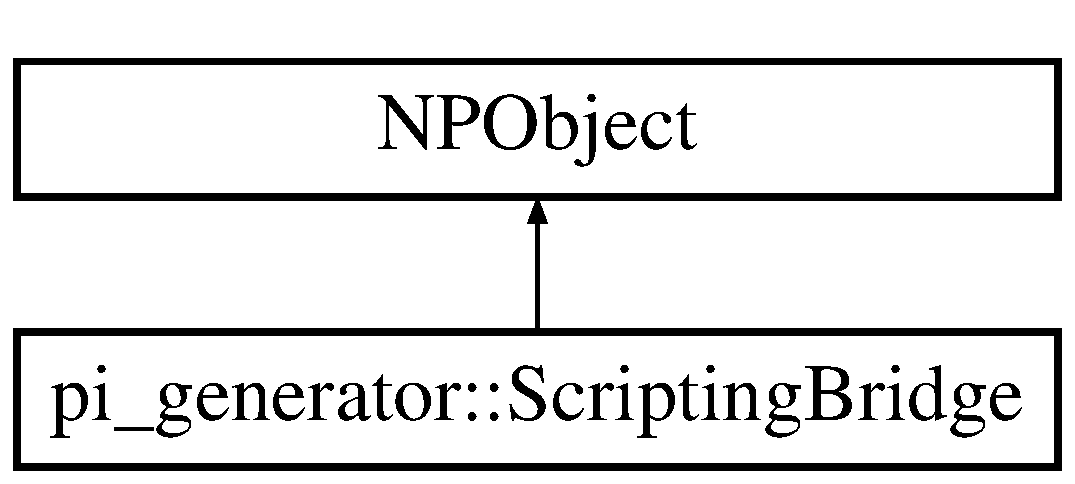
\includegraphics[height=2cm]{classpi__generator_1_1_scripting_bridge}
\end{center}
\end{figure}
\subsection*{Public Types}
\begin{DoxyCompactItemize}
\item 
typedef bool(ScriptingBridge::$\ast$ \hyperlink{classpi__generator_1_1_scripting_bridge_a48f5f7b0dfb3daabcdbfb3f7b667fd39}{Method} )(const \hyperlink{struct___n_p_variant}{NPVariant} $\ast$args, uint32\_\-t arg\_\-count, \hyperlink{struct___n_p_variant}{NPVariant} $\ast$result)
\item 
typedef bool(ScriptingBridge::$\ast$ \hyperlink{classpi__generator_1_1_scripting_bridge_abcd8cffa7f26f348e68cde316038245f}{Property} )(\hyperlink{struct___n_p_variant}{NPVariant} $\ast$result)
\end{DoxyCompactItemize}
\subsection*{Public Member Functions}
\begin{DoxyCompactItemize}
\item 
\hyperlink{classpi__generator_1_1_scripting_bridge_abcc778b6a4c482dff1ed271d7e776e42}{ScriptingBridge} (\hyperlink{struct___n_p_p}{NPP} npp)
\item 
virtual \hyperlink{classpi__generator_1_1_scripting_bridge_a605567080f40ddb9a6c2fa4ea9f2e876}{$\sim$ScriptingBridge} ()
\item 
virtual void \hyperlink{classpi__generator_1_1_scripting_bridge_a581ae88aa4acbefc30ae563452ab2fd5}{Invalidate} ()
\item 
virtual bool \hyperlink{classpi__generator_1_1_scripting_bridge_aaa99f91c8ced5df6fac0700516cdd058}{HasMethod} (\hyperlink{npruntime_8h_a3ce51391e08bd3e24128c342b1d055b9}{NPIdentifier} name)
\item 
virtual bool \hyperlink{classpi__generator_1_1_scripting_bridge_a3518781037308ae1d63bcdf5cc77a3de}{Invoke} (\hyperlink{npruntime_8h_a3ce51391e08bd3e24128c342b1d055b9}{NPIdentifier} name, const \hyperlink{struct___n_p_variant}{NPVariant} $\ast$args, uint32\_\-t arg\_\-count, \hyperlink{struct___n_p_variant}{NPVariant} $\ast$result)
\item 
virtual bool \hyperlink{classpi__generator_1_1_scripting_bridge_a0589fe559ec8b9297e37239233e238be}{InvokeDefault} (const \hyperlink{struct___n_p_variant}{NPVariant} $\ast$args, uint32\_\-t arg\_\-count, \hyperlink{struct___n_p_variant}{NPVariant} $\ast$result)
\item 
virtual bool \hyperlink{classpi__generator_1_1_scripting_bridge_a55f52d9e5e377367881e919db10b019f}{HasProperty} (\hyperlink{npruntime_8h_a3ce51391e08bd3e24128c342b1d055b9}{NPIdentifier} name)
\item 
virtual bool \hyperlink{classpi__generator_1_1_scripting_bridge_ab97693ce171c216783e79debb3b192cc}{GetProperty} (\hyperlink{npruntime_8h_a3ce51391e08bd3e24128c342b1d055b9}{NPIdentifier} name, \hyperlink{struct___n_p_variant}{NPVariant} $\ast$result)
\item 
virtual bool \hyperlink{classpi__generator_1_1_scripting_bridge_aa87ffdeb58a36a1e352814132d4a020a}{SetProperty} (\hyperlink{npruntime_8h_a3ce51391e08bd3e24128c342b1d055b9}{NPIdentifier} name, const \hyperlink{struct___n_p_variant}{NPVariant} $\ast$value)
\item 
virtual bool \hyperlink{classpi__generator_1_1_scripting_bridge_ab1a46993e1a36b9857d48776f7085aa2}{RemoveProperty} (\hyperlink{npruntime_8h_a3ce51391e08bd3e24128c342b1d055b9}{NPIdentifier} name)
\item 
bool \hyperlink{classpi__generator_1_1_scripting_bridge_afcd2c9c3e990cae2d713e8bb5d84048d}{Paint} (const \hyperlink{struct___n_p_variant}{NPVariant} $\ast$args, uint32\_\-t arg\_\-count, \hyperlink{struct___n_p_variant}{NPVariant} $\ast$result)
\end{DoxyCompactItemize}
\subsection*{Static Public Member Functions}
\begin{DoxyCompactItemize}
\item 
static bool \hyperlink{classpi__generator_1_1_scripting_bridge_a76184c7bc22d728d207e275b5f980d67}{InitializeIdentifiers} ()
\end{DoxyCompactItemize}
\subsection*{Static Public Attributes}
\begin{DoxyCompactItemize}
\item 
static \hyperlink{struct_n_p_class}{NPClass} \hyperlink{classpi__generator_1_1_scripting_bridge_a1756e8dff7625cda7697f3e9725ede25}{np\_\-class}
\end{DoxyCompactItemize}


\subsection{Detailed Description}


Definition at line 23 of file scripting\_\-bridge.h.



\subsection{Member Typedef Documentation}
\hypertarget{classpi__generator_1_1_scripting_bridge_a48f5f7b0dfb3daabcdbfb3f7b667fd39}{
\index{pi\_\-generator::ScriptingBridge@{pi\_\-generator::ScriptingBridge}!Method@{Method}}
\index{Method@{Method}!pi_generator::ScriptingBridge@{pi\_\-generator::ScriptingBridge}}
\subsubsection[{Method}]{\setlength{\rightskip}{0pt plus 5cm}typedef bool(ScriptingBridge::$\ast$ {\bf pi\_\-generator::ScriptingBridge::Method})(const {\bf NPVariant} $\ast$args, uint32\_\-t arg\_\-count, {\bf NPVariant} $\ast$result)}}
\label{classpi__generator_1_1_scripting_bridge_a48f5f7b0dfb3daabcdbfb3f7b667fd39}


Definition at line 25 of file scripting\_\-bridge.h.

\hypertarget{classpi__generator_1_1_scripting_bridge_abcd8cffa7f26f348e68cde316038245f}{
\index{pi\_\-generator::ScriptingBridge@{pi\_\-generator::ScriptingBridge}!Property@{Property}}
\index{Property@{Property}!pi_generator::ScriptingBridge@{pi\_\-generator::ScriptingBridge}}
\subsubsection[{Property}]{\setlength{\rightskip}{0pt plus 5cm}typedef bool(ScriptingBridge::$\ast$ {\bf pi\_\-generator::ScriptingBridge::Property})({\bf NPVariant} $\ast$result)}}
\label{classpi__generator_1_1_scripting_bridge_abcd8cffa7f26f348e68cde316038245f}


Definition at line 28 of file scripting\_\-bridge.h.



\subsection{Constructor \& Destructor Documentation}
\hypertarget{classpi__generator_1_1_scripting_bridge_abcc778b6a4c482dff1ed271d7e776e42}{
\index{pi\_\-generator::ScriptingBridge@{pi\_\-generator::ScriptingBridge}!ScriptingBridge@{ScriptingBridge}}
\index{ScriptingBridge@{ScriptingBridge}!pi_generator::ScriptingBridge@{pi\_\-generator::ScriptingBridge}}
\subsubsection[{ScriptingBridge}]{\setlength{\rightskip}{0pt plus 5cm}pi\_\-generator::ScriptingBridge::ScriptingBridge ({\bf NPP} {\em npp})\hspace{0.3cm}{\ttfamily  \mbox{[}inline, explicit\mbox{]}}}}
\label{classpi__generator_1_1_scripting_bridge_abcc778b6a4c482dff1ed271d7e776e42}


Definition at line 30 of file scripting\_\-bridge.h.

\hypertarget{classpi__generator_1_1_scripting_bridge_a605567080f40ddb9a6c2fa4ea9f2e876}{
\index{pi\_\-generator::ScriptingBridge@{pi\_\-generator::ScriptingBridge}!$\sim$ScriptingBridge@{$\sim$ScriptingBridge}}
\index{$\sim$ScriptingBridge@{$\sim$ScriptingBridge}!pi_generator::ScriptingBridge@{pi\_\-generator::ScriptingBridge}}
\subsubsection[{$\sim$ScriptingBridge}]{\setlength{\rightskip}{0pt plus 5cm}pi\_\-generator::ScriptingBridge::$\sim$ScriptingBridge ()\hspace{0.3cm}{\ttfamily  \mbox{[}virtual\mbox{]}}}}
\label{classpi__generator_1_1_scripting_bridge_a605567080f40ddb9a6c2fa4ea9f2e876}


Definition at line 43 of file scripting\_\-bridge.cc.



\subsection{Member Function Documentation}
\hypertarget{classpi__generator_1_1_scripting_bridge_ab97693ce171c216783e79debb3b192cc}{
\index{pi\_\-generator::ScriptingBridge@{pi\_\-generator::ScriptingBridge}!GetProperty@{GetProperty}}
\index{GetProperty@{GetProperty}!pi_generator::ScriptingBridge@{pi\_\-generator::ScriptingBridge}}
\subsubsection[{GetProperty}]{\setlength{\rightskip}{0pt plus 5cm}bool pi\_\-generator::ScriptingBridge::GetProperty ({\bf NPIdentifier} {\em name}, \/  {\bf NPVariant} $\ast$ {\em result})\hspace{0.3cm}{\ttfamily  \mbox{[}virtual\mbox{]}}}}
\label{classpi__generator_1_1_scripting_bridge_ab97693ce171c216783e79debb3b192cc}


Definition at line 64 of file scripting\_\-bridge.cc.

\hypertarget{classpi__generator_1_1_scripting_bridge_aaa99f91c8ced5df6fac0700516cdd058}{
\index{pi\_\-generator::ScriptingBridge@{pi\_\-generator::ScriptingBridge}!HasMethod@{HasMethod}}
\index{HasMethod@{HasMethod}!pi_generator::ScriptingBridge@{pi\_\-generator::ScriptingBridge}}
\subsubsection[{HasMethod}]{\setlength{\rightskip}{0pt plus 5cm}bool pi\_\-generator::ScriptingBridge::HasMethod ({\bf NPIdentifier} {\em name})\hspace{0.3cm}{\ttfamily  \mbox{[}virtual\mbox{]}}}}
\label{classpi__generator_1_1_scripting_bridge_aaa99f91c8ced5df6fac0700516cdd058}


Definition at line 48 of file scripting\_\-bridge.cc.

\hypertarget{classpi__generator_1_1_scripting_bridge_a55f52d9e5e377367881e919db10b019f}{
\index{pi\_\-generator::ScriptingBridge@{pi\_\-generator::ScriptingBridge}!HasProperty@{HasProperty}}
\index{HasProperty@{HasProperty}!pi_generator::ScriptingBridge@{pi\_\-generator::ScriptingBridge}}
\subsubsection[{HasProperty}]{\setlength{\rightskip}{0pt plus 5cm}bool pi\_\-generator::ScriptingBridge::HasProperty ({\bf NPIdentifier} {\em name})\hspace{0.3cm}{\ttfamily  \mbox{[}virtual\mbox{]}}}}
\label{classpi__generator_1_1_scripting_bridge_a55f52d9e5e377367881e919db10b019f}


Definition at line 56 of file scripting\_\-bridge.cc.

\hypertarget{classpi__generator_1_1_scripting_bridge_a76184c7bc22d728d207e275b5f980d67}{
\index{pi\_\-generator::ScriptingBridge@{pi\_\-generator::ScriptingBridge}!InitializeIdentifiers@{InitializeIdentifiers}}
\index{InitializeIdentifiers@{InitializeIdentifiers}!pi_generator::ScriptingBridge@{pi\_\-generator::ScriptingBridge}}
\subsubsection[{InitializeIdentifiers}]{\setlength{\rightskip}{0pt plus 5cm}bool pi\_\-generator::ScriptingBridge::InitializeIdentifiers ()\hspace{0.3cm}{\ttfamily  \mbox{[}static\mbox{]}}}}
\label{classpi__generator_1_1_scripting_bridge_a76184c7bc22d728d207e275b5f980d67}


Definition at line 22 of file scripting\_\-bridge.cc.

\hypertarget{classpi__generator_1_1_scripting_bridge_a581ae88aa4acbefc30ae563452ab2fd5}{
\index{pi\_\-generator::ScriptingBridge@{pi\_\-generator::ScriptingBridge}!Invalidate@{Invalidate}}
\index{Invalidate@{Invalidate}!pi_generator::ScriptingBridge@{pi\_\-generator::ScriptingBridge}}
\subsubsection[{Invalidate}]{\setlength{\rightskip}{0pt plus 5cm}void pi\_\-generator::ScriptingBridge::Invalidate ()\hspace{0.3cm}{\ttfamily  \mbox{[}virtual\mbox{]}}}}
\label{classpi__generator_1_1_scripting_bridge_a581ae88aa4acbefc30ae563452ab2fd5}


Definition at line 110 of file scripting\_\-bridge.cc.

\hypertarget{classpi__generator_1_1_scripting_bridge_a3518781037308ae1d63bcdf5cc77a3de}{
\index{pi\_\-generator::ScriptingBridge@{pi\_\-generator::ScriptingBridge}!Invoke@{Invoke}}
\index{Invoke@{Invoke}!pi_generator::ScriptingBridge@{pi\_\-generator::ScriptingBridge}}
\subsubsection[{Invoke}]{\setlength{\rightskip}{0pt plus 5cm}bool pi\_\-generator::ScriptingBridge::Invoke ({\bf NPIdentifier} {\em name}, \/  const {\bf NPVariant} $\ast$ {\em args}, \/  uint32\_\-t {\em arg\_\-count}, \/  {\bf NPVariant} $\ast$ {\em result})\hspace{0.3cm}{\ttfamily  \mbox{[}virtual\mbox{]}}}}
\label{classpi__generator_1_1_scripting_bridge_a3518781037308ae1d63bcdf5cc77a3de}


Definition at line 97 of file scripting\_\-bridge.cc.

\hypertarget{classpi__generator_1_1_scripting_bridge_a0589fe559ec8b9297e37239233e238be}{
\index{pi\_\-generator::ScriptingBridge@{pi\_\-generator::ScriptingBridge}!InvokeDefault@{InvokeDefault}}
\index{InvokeDefault@{InvokeDefault}!pi_generator::ScriptingBridge@{pi\_\-generator::ScriptingBridge}}
\subsubsection[{InvokeDefault}]{\setlength{\rightskip}{0pt plus 5cm}bool pi\_\-generator::ScriptingBridge::InvokeDefault (const {\bf NPVariant} $\ast$ {\em args}, \/  uint32\_\-t {\em arg\_\-count}, \/  {\bf NPVariant} $\ast$ {\em result})\hspace{0.3cm}{\ttfamily  \mbox{[}virtual\mbox{]}}}}
\label{classpi__generator_1_1_scripting_bridge_a0589fe559ec8b9297e37239233e238be}


Definition at line 89 of file scripting\_\-bridge.cc.

\hypertarget{classpi__generator_1_1_scripting_bridge_afcd2c9c3e990cae2d713e8bb5d84048d}{
\index{pi\_\-generator::ScriptingBridge@{pi\_\-generator::ScriptingBridge}!Paint@{Paint}}
\index{Paint@{Paint}!pi_generator::ScriptingBridge@{pi\_\-generator::ScriptingBridge}}
\subsubsection[{Paint}]{\setlength{\rightskip}{0pt plus 5cm}bool pi\_\-generator::ScriptingBridge::Paint (const {\bf NPVariant} $\ast$ {\em args}, \/  uint32\_\-t {\em arg\_\-count}, \/  {\bf NPVariant} $\ast$ {\em result})}}
\label{classpi__generator_1_1_scripting_bridge_afcd2c9c3e990cae2d713e8bb5d84048d}


Definition at line 114 of file scripting\_\-bridge.cc.

\hypertarget{classpi__generator_1_1_scripting_bridge_ab1a46993e1a36b9857d48776f7085aa2}{
\index{pi\_\-generator::ScriptingBridge@{pi\_\-generator::ScriptingBridge}!RemoveProperty@{RemoveProperty}}
\index{RemoveProperty@{RemoveProperty}!pi_generator::ScriptingBridge@{pi\_\-generator::ScriptingBridge}}
\subsubsection[{RemoveProperty}]{\setlength{\rightskip}{0pt plus 5cm}bool pi\_\-generator::ScriptingBridge::RemoveProperty ({\bf NPIdentifier} {\em name})\hspace{0.3cm}{\ttfamily  \mbox{[}virtual\mbox{]}}}}
\label{classpi__generator_1_1_scripting_bridge_ab1a46993e1a36b9857d48776f7085aa2}


Definition at line 83 of file scripting\_\-bridge.cc.

\hypertarget{classpi__generator_1_1_scripting_bridge_aa87ffdeb58a36a1e352814132d4a020a}{
\index{pi\_\-generator::ScriptingBridge@{pi\_\-generator::ScriptingBridge}!SetProperty@{SetProperty}}
\index{SetProperty@{SetProperty}!pi_generator::ScriptingBridge@{pi\_\-generator::ScriptingBridge}}
\subsubsection[{SetProperty}]{\setlength{\rightskip}{0pt plus 5cm}bool pi\_\-generator::ScriptingBridge::SetProperty ({\bf NPIdentifier} {\em name}, \/  const {\bf NPVariant} $\ast$ {\em value})\hspace{0.3cm}{\ttfamily  \mbox{[}virtual\mbox{]}}}}
\label{classpi__generator_1_1_scripting_bridge_aa87ffdeb58a36a1e352814132d4a020a}


Definition at line 77 of file scripting\_\-bridge.cc.



\subsection{Member Data Documentation}
\hypertarget{classpi__generator_1_1_scripting_bridge_a1756e8dff7625cda7697f3e9725ede25}{
\index{pi\_\-generator::ScriptingBridge@{pi\_\-generator::ScriptingBridge}!np\_\-class@{np\_\-class}}
\index{np\_\-class@{np\_\-class}!pi_generator::ScriptingBridge@{pi\_\-generator::ScriptingBridge}}
\subsubsection[{np\_\-class}]{\setlength{\rightskip}{0pt plus 5cm}{\bf NPClass} {\bf pi\_\-generator::ScriptingBridge::np\_\-class}\hspace{0.3cm}{\ttfamily  \mbox{[}static\mbox{]}}}}
\label{classpi__generator_1_1_scripting_bridge_a1756e8dff7625cda7697f3e9725ede25}
{\bfseries Initial value:}
\begin{DoxyCode}
 {
  NP_CLASS_STRUCT_VERSION,
  pi_generator::Allocate,
  pi_generator::Deallocate,
  pi_generator::Invalidate,
  pi_generator::HasMethod,
  pi_generator::Invoke,
  pi_generator::InvokeDefault,
  pi_generator::HasProperty,
  pi_generator::GetProperty,
  pi_generator::SetProperty,
  pi_generator::RemoveProperty
}
\end{DoxyCode}


Definition at line 51 of file scripting\_\-bridge.h.



The documentation for this class was generated from the following files:\begin{DoxyCompactItemize}
\item 
/home/derek/dev/cell-\/grid-\/game/nacl/crml/crml/test/pi\_\-generator/\hyperlink{test_2pi__generator_2scripting__bridge_8h}{scripting\_\-bridge.h}\item 
/home/derek/dev/cell-\/grid-\/game/nacl/crml/crml/core/\hyperlink{core_2scripting__bridge_8cc}{scripting\_\-bridge.cc}\item 
/home/derek/dev/cell-\/grid-\/game/nacl/crml/crml/test/pi\_\-generator/\hyperlink{test_2pi__generator_2scripting__bridge_8cc}{scripting\_\-bridge.cc}\end{DoxyCompactItemize}

\hypertarget{struct_test_object}{
\section{TestObject Struct Reference}
\label{struct_test_object}\index{TestObject@{TestObject}}
}


{\ttfamily \#include $<$test\_\-object.h$>$}

\subsection*{Public Attributes}
\begin{DoxyCompactItemize}
\item 
NPObject \hyperlink{struct_test_object_a23d7a50afe1b29f85b5d663cbfc763b2}{header}
\item 
NPObject $\ast$ \hyperlink{struct_test_object_a375c492938a3abf12d768b8578549861}{test\_\-object}
\end{DoxyCompactItemize}


\subsection{Detailed Description}


Definition at line 32 of file test\_\-object.h.



\subsection{Member Data Documentation}
\hypertarget{struct_test_object_a23d7a50afe1b29f85b5d663cbfc763b2}{
\index{TestObject@{TestObject}!header@{header}}
\index{header@{header}!TestObject@{TestObject}}
\subsubsection[{header}]{\setlength{\rightskip}{0pt plus 5cm}NPObject {\bf TestObject::header}}}
\label{struct_test_object_a23d7a50afe1b29f85b5d663cbfc763b2}


Definition at line 33 of file test\_\-object.h.

\hypertarget{struct_test_object_a375c492938a3abf12d768b8578549861}{
\index{TestObject@{TestObject}!test\_\-object@{test\_\-object}}
\index{test\_\-object@{test\_\-object}!TestObject@{TestObject}}
\subsubsection[{test\_\-object}]{\setlength{\rightskip}{0pt plus 5cm}NPObject $\ast$ {\bf TestObject::test\_\-object}}}
\label{struct_test_object_a375c492938a3abf12d768b8578549861}


Definition at line 34 of file test\_\-object.h.



The documentation for this struct was generated from the following files:\begin{DoxyCompactItemize}
\item 
/home/derek/dev/cell-\/grid-\/game/nacl/crml/crml/sys/\hyperlink{sys_2test__object_8h}{test\_\-object.h}\item 
/home/derek/dev/cell-\/grid-\/game/nacl/crml/crml/test/\hyperlink{test_2test__object_8h}{test\_\-object.h}\end{DoxyCompactItemize}

\hypertarget{classtumbler_1_1_tumbler}{
\section{tumbler::Tumbler Class Reference}
\label{classtumbler_1_1_tumbler}\index{tumbler::Tumbler@{tumbler::Tumbler}}
}


{\ttfamily \#include $<$tumbler.h$>$}

\subsection*{Public Member Functions}
\begin{DoxyCompactItemize}
\item 
\hyperlink{classtumbler_1_1_tumbler_a4f5dd0baa068ccb8214b0e477f7cd94b}{Tumbler} (NPP npp)
\item 
\hyperlink{classtumbler_1_1_tumbler_a80349e180aa825c15d63bada00c6e9a8}{$\sim$Tumbler} ()
\item 
NPObject $\ast$ \hyperlink{classtumbler_1_1_tumbler_ad438453c62d1edcbdd5cb39a38143a0b}{GetScriptableObject} ()
\item 
NPError \hyperlink{classtumbler_1_1_tumbler_a6aba2f3cfa10be35c0a789924343b1b0}{SetWindow} (const NPWindow \&window)
\item 
void \hyperlink{classtumbler_1_1_tumbler_ab721f5f95ce020ce6680033771ed4577}{PostRedrawNotification} ()
\item 
bool \hyperlink{classtumbler_1_1_tumbler_a8da0b0b0e85708487c55f6ca5c999da1}{DrawSelf} ()
\item 
bool \hyperlink{classtumbler_1_1_tumbler_a5e01d6cde9baab4e5c2aa4b834733bf2}{GetCameraOrientation} (float $\ast$orientation) const 
\item 
bool \hyperlink{classtumbler_1_1_tumbler_a2657d32f15492fc56406d1750172ca8c}{SetCameraOrientation} (const float $\ast$orientation)
\end{DoxyCompactItemize}


\subsection{Detailed Description}


Definition at line 38 of file tumbler.h.



\subsection{Constructor \& Destructor Documentation}
\hypertarget{classtumbler_1_1_tumbler_a4f5dd0baa068ccb8214b0e477f7cd94b}{
\index{tumbler::Tumbler@{tumbler::Tumbler}!Tumbler@{Tumbler}}
\index{Tumbler@{Tumbler}!tumbler::Tumbler@{tumbler::Tumbler}}
\subsubsection[{Tumbler}]{\setlength{\rightskip}{0pt plus 5cm}tumbler::Tumbler::Tumbler (NPP {\em npp})\hspace{0.3cm}{\ttfamily  \mbox{[}explicit\mbox{]}}}}
\label{classtumbler_1_1_tumbler_a4f5dd0baa068ccb8214b0e477f7cd94b}


Definition at line 38 of file tumbler.cc.

\hypertarget{classtumbler_1_1_tumbler_a80349e180aa825c15d63bada00c6e9a8}{
\index{tumbler::Tumbler@{tumbler::Tumbler}!$\sim$Tumbler@{$\sim$Tumbler}}
\index{$\sim$Tumbler@{$\sim$Tumbler}!tumbler::Tumbler@{tumbler::Tumbler}}
\subsubsection[{$\sim$Tumbler}]{\setlength{\rightskip}{0pt plus 5cm}tumbler::Tumbler::$\sim$Tumbler ()}}
\label{classtumbler_1_1_tumbler_a80349e180aa825c15d63bada00c6e9a8}


Definition at line 48 of file tumbler.cc.



\subsection{Member Function Documentation}
\hypertarget{classtumbler_1_1_tumbler_a8da0b0b0e85708487c55f6ca5c999da1}{
\index{tumbler::Tumbler@{tumbler::Tumbler}!DrawSelf@{DrawSelf}}
\index{DrawSelf@{DrawSelf}!tumbler::Tumbler@{tumbler::Tumbler}}
\subsubsection[{DrawSelf}]{\setlength{\rightskip}{0pt plus 5cm}bool tumbler::Tumbler::DrawSelf ()}}
\label{classtumbler_1_1_tumbler_a8da0b0b0e85708487c55f6ca5c999da1}


Definition at line 90 of file tumbler.cc.

\hypertarget{classtumbler_1_1_tumbler_a5e01d6cde9baab4e5c2aa4b834733bf2}{
\index{tumbler::Tumbler@{tumbler::Tumbler}!GetCameraOrientation@{GetCameraOrientation}}
\index{GetCameraOrientation@{GetCameraOrientation}!tumbler::Tumbler@{tumbler::Tumbler}}
\subsubsection[{GetCameraOrientation}]{\setlength{\rightskip}{0pt plus 5cm}bool tumbler::Tumbler::GetCameraOrientation (float $\ast$ {\em orientation}) const}}
\label{classtumbler_1_1_tumbler_a5e01d6cde9baab4e5c2aa4b834733bf2}


Definition at line 109 of file tumbler.cc.

\hypertarget{classtumbler_1_1_tumbler_ad438453c62d1edcbdd5cb39a38143a0b}{
\index{tumbler::Tumbler@{tumbler::Tumbler}!GetScriptableObject@{GetScriptableObject}}
\index{GetScriptableObject@{GetScriptableObject}!tumbler::Tumbler@{tumbler::Tumbler}}
\subsubsection[{GetScriptableObject}]{\setlength{\rightskip}{0pt plus 5cm}NPObject $\ast$ tumbler::Tumbler::GetScriptableObject ()}}
\label{classtumbler_1_1_tumbler_ad438453c62d1edcbdd5cb39a38143a0b}


Definition at line 60 of file tumbler.cc.

\hypertarget{classtumbler_1_1_tumbler_ab721f5f95ce020ce6680033771ed4577}{
\index{tumbler::Tumbler@{tumbler::Tumbler}!PostRedrawNotification@{PostRedrawNotification}}
\index{PostRedrawNotification@{PostRedrawNotification}!tumbler::Tumbler@{tumbler::Tumbler}}
\subsubsection[{PostRedrawNotification}]{\setlength{\rightskip}{0pt plus 5cm}void tumbler::Tumbler::PostRedrawNotification ()}}
\label{classtumbler_1_1_tumbler_ab721f5f95ce020ce6680033771ed4577}


Definition at line 86 of file tumbler.cc.

\hypertarget{classtumbler_1_1_tumbler_a2657d32f15492fc56406d1750172ca8c}{
\index{tumbler::Tumbler@{tumbler::Tumbler}!SetCameraOrientation@{SetCameraOrientation}}
\index{SetCameraOrientation@{SetCameraOrientation}!tumbler::Tumbler@{tumbler::Tumbler}}
\subsubsection[{SetCameraOrientation}]{\setlength{\rightskip}{0pt plus 5cm}bool tumbler::Tumbler::SetCameraOrientation (const float $\ast$ {\em orientation})}}
\label{classtumbler_1_1_tumbler_a2657d32f15492fc56406d1750172ca8c}


Definition at line 117 of file tumbler.cc.

\hypertarget{classtumbler_1_1_tumbler_a6aba2f3cfa10be35c0a789924343b1b0}{
\index{tumbler::Tumbler@{tumbler::Tumbler}!SetWindow@{SetWindow}}
\index{SetWindow@{SetWindow}!tumbler::Tumbler@{tumbler::Tumbler}}
\subsubsection[{SetWindow}]{\setlength{\rightskip}{0pt plus 5cm}NPError tumbler::Tumbler::SetWindow (const NPWindow \& {\em window})}}
\label{classtumbler_1_1_tumbler_a6aba2f3cfa10be35c0a789924343b1b0}


Definition at line 71 of file tumbler.cc.



The documentation for this class was generated from the following files:\begin{DoxyCompactItemize}
\item 
/home/derek/dev/crml/crml/lib/tumbler/\hyperlink{tumbler_8h}{tumbler.h}\item 
/home/derek/dev/crml/crml/lib/tumbler/\hyperlink{tumbler_8cc}{tumbler.cc}\end{DoxyCompactItemize}

\hypertarget{structtumbler_1_1_tumbler_context3_d}{
\section{tumbler::TumblerContext3D Struct Reference}
\label{structtumbler_1_1_tumbler_context3_d}\index{tumbler::TumblerContext3D@{tumbler::TumblerContext3D}}
}


{\ttfamily \#include $<$tumbler.h$>$}

\subsection*{Public Attributes}
\begin{DoxyCompactItemize}
\item 
void $\ast$ \hyperlink{structtumbler_1_1_tumbler_context3_d_a1274a5b24b002c4e264bc7ee9298e85d}{user\_\-data\_\-}
\end{DoxyCompactItemize}


\subsection{Detailed Description}


Definition at line 34 of file tumbler.h.



\subsection{Member Data Documentation}
\hypertarget{structtumbler_1_1_tumbler_context3_d_a1274a5b24b002c4e264bc7ee9298e85d}{
\index{tumbler::TumblerContext3D@{tumbler::TumblerContext3D}!user\_\-data\_\-@{user\_\-data\_\-}}
\index{user\_\-data\_\-@{user\_\-data\_\-}!tumbler::TumblerContext3D@{tumbler::TumblerContext3D}}
\subsubsection[{user\_\-data\_\-}]{\setlength{\rightskip}{0pt plus 5cm}void$\ast$ {\bf tumbler::TumblerContext3D::user\_\-data\_\-}}}
\label{structtumbler_1_1_tumbler_context3_d_a1274a5b24b002c4e264bc7ee9298e85d}


Definition at line 35 of file tumbler.h.



The documentation for this struct was generated from the following file:\begin{DoxyCompactItemize}
\item 
/home/derek/dev/crml/crml/lib/tumbler/\hyperlink{tumbler_8h}{tumbler.h}\end{DoxyCompactItemize}

\chapter{File Documentation}
\hypertarget{hello_8cc}{
\section{/home/derek/dev/cell-\/grid-\/game/nacl/crml/crml/build/hello.cc File Reference}
\label{hello_8cc}\index{/home/derek/dev/cell-\/grid-\/game/nacl/crml/crml/build/hello.cc@{/home/derek/dev/cell-\/grid-\/game/nacl/crml/crml/build/hello.cc}}
}
{\ttfamily \#include $<$iostream$>$}\par
\subsection*{Functions}
\begin{DoxyCompactItemize}
\item 
std::string \hyperlink{hello_8cc_ad922e75020deee80170f86f860b5905a}{hexdecode} (std::string)
\item 
int \hyperlink{hello_8cc_ae66f6b31b5ad750f1fe042a706a4e3d4}{main} ()
\end{DoxyCompactItemize}


\subsection{Function Documentation}
\hypertarget{hello_8cc_ad922e75020deee80170f86f860b5905a}{
\index{hello.cc@{hello.cc}!hexdecode@{hexdecode}}
\index{hexdecode@{hexdecode}!hello.cc@{hello.cc}}
\subsubsection[{hexdecode}]{\setlength{\rightskip}{0pt plus 5cm}std::string hexdecode (std::string)}}
\label{hello_8cc_ad922e75020deee80170f86f860b5905a}


Definition at line 46 of file hexdecode.cc.

\hypertarget{hello_8cc_ae66f6b31b5ad750f1fe042a706a4e3d4}{
\index{hello.cc@{hello.cc}!main@{main}}
\index{main@{main}!hello.cc@{hello.cc}}
\subsubsection[{main}]{\setlength{\rightskip}{0pt plus 5cm}int main ()}}
\label{hello_8cc_ae66f6b31b5ad750f1fe042a706a4e3d4}


Definition at line 5 of file hello.cc.


\hypertarget{core_8h}{
\section{/home/derek/dev/cell-\/grid-\/game/nacl/crml/crml/core/core.h File Reference}
\label{core_8h}\index{/home/derek/dev/cell-\/grid-\/game/nacl/crml/crml/core/core.h@{/home/derek/dev/cell-\/grid-\/game/nacl/crml/crml/core/core.h}}
}
\subsection*{Classes}
\begin{DoxyCompactItemize}
\item 
class \hyperlink{classcrml_1_1_core}{crml::Core}
\begin{DoxyCompactList}\small\item\em The \hyperlink{classcrml_1_1_core}{Core} object which wires all subsystems and maintains an open channel with javascript. \item\end{DoxyCompactList}\end{DoxyCompactItemize}
\subsection*{Namespaces}
\begin{DoxyCompactItemize}
\item 
namespace \hyperlink{namespacecrml}{crml}
\end{DoxyCompactItemize}

\hypertarget{nacl__macros_8h}{
\section{/home/derek/dev/cell-\/grid-\/game/nacl/crml/crml/core/nacl\_\-macros.h File Reference}
\label{nacl__macros_8h}\index{/home/derek/dev/cell-\/grid-\/game/nacl/crml/crml/core/nacl\_\-macros.h@{/home/derek/dev/cell-\/grid-\/game/nacl/crml/crml/core/nacl\_\-macros.h}}
}
{\ttfamily \#include $<$stdlib.h$>$}\par
\subsection*{Defines}
\begin{DoxyCompactItemize}
\item 
\#define \hyperlink{nacl__macros_8h_adf354c0329c28f6c403e56848dd9d2df}{NACL\_\-ARRAY\_\-SIZE\_\-UNSAFE}(arr)~((sizeof arr)/sizeof arr\mbox{[}0\mbox{]})
\item 
\#define \hyperlink{nacl__macros_8h_a5c932ef314189f0a509d279a83c949a4}{NACL\_\-ASSERT\_\-IS\_\-ARRAY}(arr)
\item 
\#define \hyperlink{nacl__macros_8h_ae4c39134b9463bd7ba877e0d812fdf6b}{NACL\_\-ARRAY\_\-SIZE}(arr)~NACL\_\-ARRAY\_\-SIZE\_\-UNSAFE(arr)
\item 
\#define \hyperlink{nacl__macros_8h_a23263f5965a3c42982bcfd35b160b2e6}{NACL\_\-ASSERT\_\-IS\_\-POINTER}(ptr)~do \{ if (0) \{ ++ptr; \} \} while (0)
\item 
\#define \hyperlink{nacl__macros_8h_a03dfabcb731517256cc8037301a4bbf6}{NACL\_\-ASSERT\_\-SAME\_\-SIZE}(t1, t2)
\item 
\#define \hyperlink{nacl__macros_8h_af099bc858885cc07068796b91997177d}{NACL\_\-UMAX\_\-VAL}(T)~((T) -\/1)
\item 
\#define \hyperlink{nacl__macros_8h_a16169ad0458b172a2ef2a3ad79233ee5}{NACL\_\-MAX\_\-VAL}(T)~((T) (((u \#\# T) -\/1) $>$$>$ 1))
\item 
\#define \hyperlink{nacl__macros_8h_a8700a419c98364b6f8d13c3ffa200cfc}{NACL\_\-UMIN\_\-VAL}(T)~((T) 0)
\item 
\#define \hyperlink{nacl__macros_8h_aa301cbfdf6debc8102ff99e381c3d857}{NACL\_\-MIN\_\-VAL}(T)~((T) $\sim$NACL\_\-MAX\_\-VAL(T))
\item 
\#define \hyperlink{nacl__macros_8h_a5595c5e0048ed5698c0eeef3fd2468ca}{NACL\_\-NANOS\_\-PER\_\-MICRO}~1000
\item 
\#define \hyperlink{nacl__macros_8h_a96fba197fc9829fba81ab0ecbf2ed044}{NACL\_\-100\_\-NANOS\_\-PER\_\-MILLI}~(10 $\ast$ 1000)
\item 
\#define \hyperlink{nacl__macros_8h_adc3779b215d4284406a7e4c58773c44d}{NACL\_\-NANOS\_\-PER\_\-MILLI}~(1000 $\ast$ 1000)
\item 
\#define \hyperlink{nacl__macros_8h_a83a1e567faa9c215885c0a096fffd77a}{NACL\_\-MICROS\_\-PER\_\-UNIT}~(1000 $\ast$ 1000)
\item 
\#define \hyperlink{nacl__macros_8h_affb63becc478fef278629abae0b22fc5}{NACL\_\-MILLIS\_\-PER\_\-UNIT}~1000
\item 
\#define \hyperlink{nacl__macros_8h_aed31fc49401725e4b6767ffdfead336f}{NACL\_\-UNIT\_\-CONVERT\_\-ROUND}(v, m)~(((v) + (m) -\/ 1)/(m))
\end{DoxyCompactItemize}


\subsection{Define Documentation}
\hypertarget{nacl__macros_8h_a96fba197fc9829fba81ab0ecbf2ed044}{
\index{nacl\_\-macros.h@{nacl\_\-macros.h}!NACL\_\-100\_\-NANOS\_\-PER\_\-MILLI@{NACL\_\-100\_\-NANOS\_\-PER\_\-MILLI}}
\index{NACL\_\-100\_\-NANOS\_\-PER\_\-MILLI@{NACL\_\-100\_\-NANOS\_\-PER\_\-MILLI}!nacl_macros.h@{nacl\_\-macros.h}}
\subsubsection[{NACL\_\-100\_\-NANOS\_\-PER\_\-MILLI}]{\setlength{\rightskip}{0pt plus 5cm}\#define NACL\_\-100\_\-NANOS\_\-PER\_\-MILLI~(10 $\ast$ 1000)}}
\label{nacl__macros_8h_a96fba197fc9829fba81ab0ecbf2ed044}


Definition at line 211 of file nacl\_\-macros.h.

\hypertarget{nacl__macros_8h_ae4c39134b9463bd7ba877e0d812fdf6b}{
\index{nacl\_\-macros.h@{nacl\_\-macros.h}!NACL\_\-ARRAY\_\-SIZE@{NACL\_\-ARRAY\_\-SIZE}}
\index{NACL\_\-ARRAY\_\-SIZE@{NACL\_\-ARRAY\_\-SIZE}!nacl_macros.h@{nacl\_\-macros.h}}
\subsubsection[{NACL\_\-ARRAY\_\-SIZE}]{\setlength{\rightskip}{0pt plus 5cm}\#define NACL\_\-ARRAY\_\-SIZE(arr)~NACL\_\-ARRAY\_\-SIZE\_\-UNSAFE(arr)}}
\label{nacl__macros_8h_ae4c39134b9463bd7ba877e0d812fdf6b}


Definition at line 158 of file nacl\_\-macros.h.

\hypertarget{nacl__macros_8h_adf354c0329c28f6c403e56848dd9d2df}{
\index{nacl\_\-macros.h@{nacl\_\-macros.h}!NACL\_\-ARRAY\_\-SIZE\_\-UNSAFE@{NACL\_\-ARRAY\_\-SIZE\_\-UNSAFE}}
\index{NACL\_\-ARRAY\_\-SIZE\_\-UNSAFE@{NACL\_\-ARRAY\_\-SIZE\_\-UNSAFE}!nacl_macros.h@{nacl\_\-macros.h}}
\subsubsection[{NACL\_\-ARRAY\_\-SIZE\_\-UNSAFE}]{\setlength{\rightskip}{0pt plus 5cm}\#define NACL\_\-ARRAY\_\-SIZE\_\-UNSAFE(arr)~((sizeof arr)/sizeof arr\mbox{[}0\mbox{]})}}
\label{nacl__macros_8h_adf354c0329c28f6c403e56848dd9d2df}


Definition at line 20 of file nacl\_\-macros.h.

\hypertarget{nacl__macros_8h_a5c932ef314189f0a509d279a83c949a4}{
\index{nacl\_\-macros.h@{nacl\_\-macros.h}!NACL\_\-ASSERT\_\-IS\_\-ARRAY@{NACL\_\-ASSERT\_\-IS\_\-ARRAY}}
\index{NACL\_\-ASSERT\_\-IS\_\-ARRAY@{NACL\_\-ASSERT\_\-IS\_\-ARRAY}!nacl_macros.h@{nacl\_\-macros.h}}
\subsubsection[{NACL\_\-ASSERT\_\-IS\_\-ARRAY}]{\setlength{\rightskip}{0pt plus 5cm}\#define NACL\_\-ASSERT\_\-IS\_\-ARRAY(arr)}}
\label{nacl__macros_8h_a5c932ef314189f0a509d279a83c949a4}


Definition at line 157 of file nacl\_\-macros.h.

\hypertarget{nacl__macros_8h_a23263f5965a3c42982bcfd35b160b2e6}{
\index{nacl\_\-macros.h@{nacl\_\-macros.h}!NACL\_\-ASSERT\_\-IS\_\-POINTER@{NACL\_\-ASSERT\_\-IS\_\-POINTER}}
\index{NACL\_\-ASSERT\_\-IS\_\-POINTER@{NACL\_\-ASSERT\_\-IS\_\-POINTER}!nacl_macros.h@{nacl\_\-macros.h}}
\subsubsection[{NACL\_\-ASSERT\_\-IS\_\-POINTER}]{\setlength{\rightskip}{0pt plus 5cm}\#define NACL\_\-ASSERT\_\-IS\_\-POINTER(ptr)~do \{ if (0) \{ ++ptr; \} \} while (0)}}
\label{nacl__macros_8h_a23263f5965a3c42982bcfd35b160b2e6}


Definition at line 168 of file nacl\_\-macros.h.

\hypertarget{nacl__macros_8h_a03dfabcb731517256cc8037301a4bbf6}{
\index{nacl\_\-macros.h@{nacl\_\-macros.h}!NACL\_\-ASSERT\_\-SAME\_\-SIZE@{NACL\_\-ASSERT\_\-SAME\_\-SIZE}}
\index{NACL\_\-ASSERT\_\-SAME\_\-SIZE@{NACL\_\-ASSERT\_\-SAME\_\-SIZE}!nacl_macros.h@{nacl\_\-macros.h}}
\subsubsection[{NACL\_\-ASSERT\_\-SAME\_\-SIZE}]{\setlength{\rightskip}{0pt plus 5cm}\#define NACL\_\-ASSERT\_\-SAME\_\-SIZE(t1, \/  t2)}}
\label{nacl__macros_8h_a03dfabcb731517256cc8037301a4bbf6}
{\bfseries Value:}
\begin{DoxyCode}
do { char tested_types_are_not_the_same_size[sizeof(t1) == sizeof(t2)]; \
       (void) tested_types_are_not_the_same_size; } while (0)
\end{DoxyCode}


Definition at line 179 of file nacl\_\-macros.h.

\hypertarget{nacl__macros_8h_a16169ad0458b172a2ef2a3ad79233ee5}{
\index{nacl\_\-macros.h@{nacl\_\-macros.h}!NACL\_\-MAX\_\-VAL@{NACL\_\-MAX\_\-VAL}}
\index{NACL\_\-MAX\_\-VAL@{NACL\_\-MAX\_\-VAL}!nacl_macros.h@{nacl\_\-macros.h}}
\subsubsection[{NACL\_\-MAX\_\-VAL}]{\setlength{\rightskip}{0pt plus 5cm}\#define NACL\_\-MAX\_\-VAL(T)~((T) (((u \#\# T) -\/1) $>$$>$ 1))}}
\label{nacl__macros_8h_a16169ad0458b172a2ef2a3ad79233ee5}


Definition at line 201 of file nacl\_\-macros.h.

\hypertarget{nacl__macros_8h_a83a1e567faa9c215885c0a096fffd77a}{
\index{nacl\_\-macros.h@{nacl\_\-macros.h}!NACL\_\-MICROS\_\-PER\_\-UNIT@{NACL\_\-MICROS\_\-PER\_\-UNIT}}
\index{NACL\_\-MICROS\_\-PER\_\-UNIT@{NACL\_\-MICROS\_\-PER\_\-UNIT}!nacl_macros.h@{nacl\_\-macros.h}}
\subsubsection[{NACL\_\-MICROS\_\-PER\_\-UNIT}]{\setlength{\rightskip}{0pt plus 5cm}\#define NACL\_\-MICROS\_\-PER\_\-UNIT~(1000 $\ast$ 1000)}}
\label{nacl__macros_8h_a83a1e567faa9c215885c0a096fffd77a}


Definition at line 213 of file nacl\_\-macros.h.

\hypertarget{nacl__macros_8h_affb63becc478fef278629abae0b22fc5}{
\index{nacl\_\-macros.h@{nacl\_\-macros.h}!NACL\_\-MILLIS\_\-PER\_\-UNIT@{NACL\_\-MILLIS\_\-PER\_\-UNIT}}
\index{NACL\_\-MILLIS\_\-PER\_\-UNIT@{NACL\_\-MILLIS\_\-PER\_\-UNIT}!nacl_macros.h@{nacl\_\-macros.h}}
\subsubsection[{NACL\_\-MILLIS\_\-PER\_\-UNIT}]{\setlength{\rightskip}{0pt plus 5cm}\#define NACL\_\-MILLIS\_\-PER\_\-UNIT~1000}}
\label{nacl__macros_8h_affb63becc478fef278629abae0b22fc5}


Definition at line 214 of file nacl\_\-macros.h.

\hypertarget{nacl__macros_8h_aa301cbfdf6debc8102ff99e381c3d857}{
\index{nacl\_\-macros.h@{nacl\_\-macros.h}!NACL\_\-MIN\_\-VAL@{NACL\_\-MIN\_\-VAL}}
\index{NACL\_\-MIN\_\-VAL@{NACL\_\-MIN\_\-VAL}!nacl_macros.h@{nacl\_\-macros.h}}
\subsubsection[{NACL\_\-MIN\_\-VAL}]{\setlength{\rightskip}{0pt plus 5cm}\#define NACL\_\-MIN\_\-VAL(T)~((T) $\sim$NACL\_\-MAX\_\-VAL(T))}}
\label{nacl__macros_8h_aa301cbfdf6debc8102ff99e381c3d857}


Definition at line 203 of file nacl\_\-macros.h.

\hypertarget{nacl__macros_8h_a5595c5e0048ed5698c0eeef3fd2468ca}{
\index{nacl\_\-macros.h@{nacl\_\-macros.h}!NACL\_\-NANOS\_\-PER\_\-MICRO@{NACL\_\-NANOS\_\-PER\_\-MICRO}}
\index{NACL\_\-NANOS\_\-PER\_\-MICRO@{NACL\_\-NANOS\_\-PER\_\-MICRO}!nacl_macros.h@{nacl\_\-macros.h}}
\subsubsection[{NACL\_\-NANOS\_\-PER\_\-MICRO}]{\setlength{\rightskip}{0pt plus 5cm}\#define NACL\_\-NANOS\_\-PER\_\-MICRO~1000}}
\label{nacl__macros_8h_a5595c5e0048ed5698c0eeef3fd2468ca}


Definition at line 210 of file nacl\_\-macros.h.

\hypertarget{nacl__macros_8h_adc3779b215d4284406a7e4c58773c44d}{
\index{nacl\_\-macros.h@{nacl\_\-macros.h}!NACL\_\-NANOS\_\-PER\_\-MILLI@{NACL\_\-NANOS\_\-PER\_\-MILLI}}
\index{NACL\_\-NANOS\_\-PER\_\-MILLI@{NACL\_\-NANOS\_\-PER\_\-MILLI}!nacl_macros.h@{nacl\_\-macros.h}}
\subsubsection[{NACL\_\-NANOS\_\-PER\_\-MILLI}]{\setlength{\rightskip}{0pt plus 5cm}\#define NACL\_\-NANOS\_\-PER\_\-MILLI~(1000 $\ast$ 1000)}}
\label{nacl__macros_8h_adc3779b215d4284406a7e4c58773c44d}


Definition at line 212 of file nacl\_\-macros.h.

\hypertarget{nacl__macros_8h_af099bc858885cc07068796b91997177d}{
\index{nacl\_\-macros.h@{nacl\_\-macros.h}!NACL\_\-UMAX\_\-VAL@{NACL\_\-UMAX\_\-VAL}}
\index{NACL\_\-UMAX\_\-VAL@{NACL\_\-UMAX\_\-VAL}!nacl_macros.h@{nacl\_\-macros.h}}
\subsubsection[{NACL\_\-UMAX\_\-VAL}]{\setlength{\rightskip}{0pt plus 5cm}\#define NACL\_\-UMAX\_\-VAL(T)~((T) -\/1)}}
\label{nacl__macros_8h_af099bc858885cc07068796b91997177d}


Definition at line 200 of file nacl\_\-macros.h.

\hypertarget{nacl__macros_8h_a8700a419c98364b6f8d13c3ffa200cfc}{
\index{nacl\_\-macros.h@{nacl\_\-macros.h}!NACL\_\-UMIN\_\-VAL@{NACL\_\-UMIN\_\-VAL}}
\index{NACL\_\-UMIN\_\-VAL@{NACL\_\-UMIN\_\-VAL}!nacl_macros.h@{nacl\_\-macros.h}}
\subsubsection[{NACL\_\-UMIN\_\-VAL}]{\setlength{\rightskip}{0pt plus 5cm}\#define NACL\_\-UMIN\_\-VAL(T)~((T) 0)}}
\label{nacl__macros_8h_a8700a419c98364b6f8d13c3ffa200cfc}


Definition at line 202 of file nacl\_\-macros.h.

\hypertarget{nacl__macros_8h_aed31fc49401725e4b6767ffdfead336f}{
\index{nacl\_\-macros.h@{nacl\_\-macros.h}!NACL\_\-UNIT\_\-CONVERT\_\-ROUND@{NACL\_\-UNIT\_\-CONVERT\_\-ROUND}}
\index{NACL\_\-UNIT\_\-CONVERT\_\-ROUND@{NACL\_\-UNIT\_\-CONVERT\_\-ROUND}!nacl_macros.h@{nacl\_\-macros.h}}
\subsubsection[{NACL\_\-UNIT\_\-CONVERT\_\-ROUND}]{\setlength{\rightskip}{0pt plus 5cm}\#define NACL\_\-UNIT\_\-CONVERT\_\-ROUND(v, \/  m)~(((v) + (m) -\/ 1)/(m))}}
\label{nacl__macros_8h_aed31fc49401725e4b6767ffdfead336f}


Definition at line 215 of file nacl\_\-macros.h.


\hypertarget{nacl__syscalls_8h}{
\section{/home/derek/dev/cell-\/grid-\/game/nacl/crml/crml/core/nacl\_\-syscalls.h File Reference}
\label{nacl__syscalls_8h}\index{/home/derek/dev/cell-\/grid-\/game/nacl/crml/crml/core/nacl\_\-syscalls.h@{/home/derek/dev/cell-\/grid-\/game/nacl/crml/crml/core/nacl\_\-syscalls.h}}
}
{\ttfamily \#include $<$sys/types.h$>$}\par
{\ttfamily \#include $<$sys/stat.h$>$}\par
{\ttfamily \#include $<$time.h$>$}\par
\subsection*{Functions}
\begin{DoxyCompactItemize}
\item 
void \hyperlink{group__syscalls_ga4430741655c04cf7d609fd935f52a28a}{null\_\-syscall} (void)
\item 
int \hyperlink{group__syscalls_ga0bc065c5cd7178fb88c67a4d02f61deb}{open} (char const $\ast$pathname, int flags,...)
\item 
int \hyperlink{group__syscalls_gab919bda3c5fc0afcf6e3417b840da6e9}{close} (int desc)
\item 
int \hyperlink{group__syscalls_ga709fa54ec765f9f1702f48b43d875a08}{read} (int desc, void $\ast$buf, size\_\-t count)
\item 
int \hyperlink{group__syscalls_ga3b0897fd20782dd7792b88d189e9d4df}{write} (int desc, void const $\ast$buf, size\_\-t count)
\item 
off\_\-t \hyperlink{group__syscalls_gab953b420ed5fc8595d05e52d5bc5a474}{lseek} (int desc, off\_\-t offset, int whence)
\item 
int \hyperlink{group__syscalls_ga546661554019fd9554cf4526305c24fd}{ioctl} (int desc, int request, void $\ast$arg)
\item 
void $\ast$ \hyperlink{group__syscalls_gafdb60e6e9d2dd663e3cc8a13ef796877}{sysbrk} (void $\ast$new\_\-break)
\item 
void $\ast$ \hyperlink{group__syscalls_ga8937a334d42232a0804ed450bb3b8e27}{mmap} (void $\ast$start, size\_\-t length, int prot, int flags, int desc, off\_\-t offset)
\item 
int \hyperlink{group__syscalls_ga559e66a4492a6cb9c6ef5cd07edb8955}{munmap} (void $\ast$start, size\_\-t length)
\item 
void \hyperlink{group__syscalls_gabc96bd69b58b2deaddb484478d911c1b}{\_\-exit} (int status)
\item 
void \hyperlink{group__syscalls_ga87c2438941819bb3cc31658aa9eb66fe}{thread\_\-exit} (void)
\item 
int \hyperlink{group__syscalls_ga2f316a4ad94a242df56b01953677015d}{gettimeofday} (struct timeval $\ast$tv, void $\ast$tz)
\item 
clock\_\-t \hyperlink{group__syscalls_gade863cfcca9ee19f20ca95796f8ddc1e}{clock} (void)
\item 
int \hyperlink{group__syscalls_ga1b63fa141b202a0b01cfef8421aa48d6}{nanosleep} (const struct timespec $\ast$req, struct timespec $\ast$rem)
\item 
int \hyperlink{group__syscalls_ga3dc1b07404b646712a144e2057359876}{stat} (const char $\ast$path, struct stat $\ast$buf)
\item 
int \hyperlink{group__syscalls_ga09d2f0c23245cbe6d78e532bbb7644a0}{srpc\_\-get\_\-fd} (void)
\item 
int \hyperlink{group__syscalls_ga860564306c0be29e7894d9633f866ab8}{imc\_\-makeboundsock} (int sock\_\-and\_\-addr\mbox{[}2\mbox{]})
\item 
int \hyperlink{group__syscalls_gab16585276c20a165a3b70df3eb7b21b8}{imc\_\-accept} (int desc)
\item 
int \hyperlink{group__syscalls_ga8d0d3a853d9db5850b9996111a81455c}{imc\_\-connect} (int desc)
\item 
int \hyperlink{group__syscalls_gaeebbaffd8770c75e4cd8648621dc2e77}{imc\_\-sendmsg} (int desc, struct NaClImcMsgHdr const $\ast$nmhp, int flags)
\item 
int \hyperlink{group__syscalls_gac935e49fda12e4f012fcb9eea3475f5c}{imc\_\-recvmsg} (int desc, struct NaClImcMsgHdr $\ast$nmhp, int flags)
\item 
int \hyperlink{group__syscalls_ga182a6da37d09ec51dcd181dd5a393fba}{imc\_\-mem\_\-obj\_\-create} (size\_\-t nbytes)
\item 
int \hyperlink{group__syscalls_ga80848569a6564f83a78a2975af2e621f}{imc\_\-socketpair} (int pair\mbox{[}2\mbox{]})
\item 
int \hyperlink{group__syscalls_ga357cd4b34c13011749dfffb42b489f09}{sched\_\-yield} (void)
\item 
int \hyperlink{group__syscalls_ga0767bb3577482bd018fad742f12fd35a}{nacl\_\-dyncode\_\-copy} (void $\ast$dest, const void $\ast$src, size\_\-t size)
\end{DoxyCompactItemize}


\subsection{Detailed Description}
Defines \href{group__syscalls.html}{\tt Service Runtime Calls}. The ABI is implicitly defined. 

Definition in file \hyperlink{nacl__syscalls_8h_source}{nacl\_\-syscalls.h}.


\hypertarget{npapi_8h}{
\section{/home/derek/dev/cell-\/grid-\/game/nacl/crml/crml/core/npapi.h File Reference}
\label{npapi_8h}\index{/home/derek/dev/cell-\/grid-\/game/nacl/crml/crml/core/npapi.h@{/home/derek/dev/cell-\/grid-\/game/nacl/crml/crml/core/npapi.h}}
}
{\ttfamily \#include \char`\"{}nptypes.h\char`\"{}}\par
{\ttfamily \#include \char`\"{}base/basictypes.h\char`\"{}}\par
\subsection*{Classes}
\begin{DoxyCompactItemize}
\item 
struct \hyperlink{struct___n_p_p}{\_\-NPP}
\item 
struct \hyperlink{struct___n_p_stream}{\_\-NPStream}
\item 
struct \hyperlink{struct___n_p_byte_range}{\_\-NPByteRange}
\item 
struct \hyperlink{struct___n_p_saved_data}{\_\-NPSavedData}
\item 
struct \hyperlink{struct___n_p_rect}{\_\-NPRect}
\item 
struct \hyperlink{struct___n_p_size}{\_\-NPSize}
\item 
struct \hyperlink{struct___n_p_window}{\_\-NPWindow}
\item 
struct \hyperlink{struct___n_p_image_expose}{\_\-NPImageExpose}
\item 
struct \hyperlink{struct___n_p_full_print}{\_\-NPFullPrint}
\item 
struct \hyperlink{struct___n_p_embed_print}{\_\-NPEmbedPrint}
\item 
struct \hyperlink{struct___n_p_print}{\_\-NPPrint}
\end{DoxyCompactItemize}
\subsection*{Defines}
\begin{DoxyCompactItemize}
\item 
\#define \hyperlink{npapi_8h_ab47457c1e7904b9dfa7c18e8c76a5f89}{NP\_\-VERSION\_\-MAJOR}~0
\item 
\#define \hyperlink{npapi_8h_a6eef261b755a9ebbf594d6605e43eb88}{NP\_\-VERSION\_\-MINOR}~23
\item 
\#define \hyperlink{npapi_8h_a590263a039d0a19f89efc92a3b0a08db}{NP\_\-INFO\_\-ProductVersion}~1
\item 
\#define \hyperlink{npapi_8h_a4ed3322968f34638a15746b93054464d}{NP\_\-INFO\_\-MIMEType}~2
\item 
\#define \hyperlink{npapi_8h_ae5382c6f6cfb8fafbd3e453d5f1a7f49}{NP\_\-INFO\_\-FileOpenName}~3
\item 
\#define \hyperlink{npapi_8h_ae71364168aee8580f1f41d882ebfa151}{NP\_\-INFO\_\-FileExtents}~4
\item 
\#define \hyperlink{npapi_8h_a5f56f2dc6cae93f7be261b802ba6ad69}{NP\_\-INFO\_\-FileDescription}~5
\item 
\#define \hyperlink{npapi_8h_a5b25023189682f1b13108f6013d37cf3}{NP\_\-INFO\_\-ProductName}~6
\item 
\#define \hyperlink{npapi_8h_a2dda813211ff61f6308b107cb4cb51fb}{NP\_\-INFO\_\-CompanyName}~7
\item 
\#define \hyperlink{npapi_8h_a61317bef320a3cc8c139ebc3a8a8e3b6}{NP\_\-INFO\_\-FileVersion}~8
\item 
\#define \hyperlink{npapi_8h_ae7b3cf8fbd53ed73bf244142bc96ba58}{NP\_\-INFO\_\-InternalName}~9
\item 
\#define \hyperlink{npapi_8h_a1bbe7ba66da129de6cc1a1a701325af7}{NP\_\-INFO\_\-LegalCopyright}~10
\item 
\#define \hyperlink{npapi_8h_a7f86e98a9668fa83c4c855ca0acfe7a3}{NP\_\-INFO\_\-OriginalFilename}~11
\item 
\#define \hyperlink{npapi_8h_a82943ecb6df2e55db7bf17220802a07f}{kNPEventNotHandled}~0
\item 
\#define \hyperlink{npapi_8h_ad2b7bf24d627055e8e03c1b80f2e359c}{kNPEventHandled}~1
\item 
\#define \hyperlink{npapi_8h_aafa8dbb0b2b95bcc7dbb8e6f4723535d}{kNPEventStartIME}~2
\item 
\#define \hyperlink{npapi_8h_a5dd6bd57a666e694b46601b2dc339f62}{NP\_\-ABI\_\-GCC3\_\-MASK}~0x10000000
\item 
\#define \hyperlink{npapi_8h_a942625c4ee32c820694213952a867e0f}{\_\-NP\_\-ABI\_\-MIXIN\_\-FOR\_\-GCC3}~0
\item 
\#define \hyperlink{npapi_8h_ad9bcf10196e71201d37c9b614026b9d1}{\_\-NP\_\-ABI\_\-MIXIN\_\-FOR\_\-MACHO}~0
\item 
\#define \hyperlink{npapi_8h_a696786d809cb2d524d8a06a7e504acd3}{NP\_\-ABI\_\-MASK}~(\_\-NP\_\-ABI\_\-MIXIN\_\-FOR\_\-GCC3 $|$ \_\-NP\_\-ABI\_\-MIXIN\_\-FOR\_\-MACHO)
\item 
\#define \hyperlink{npapi_8h_ab8578fcf4424b3b2125925d63fa0b8a1}{NP\_\-EMBED}~1
\item 
\#define \hyperlink{npapi_8h_a36ccc978c591253b34651f04089d8345}{NP\_\-FULL}~2
\item 
\#define \hyperlink{npapi_8h_a2dac9ddf9cbf9ac5fe0737e5e60d961d}{NP\_\-NORMAL}~1
\item 
\#define \hyperlink{npapi_8h_ab4c6989a49ac0081db1b5d0ca41bb445}{NP\_\-SEEK}~2
\item 
\#define \hyperlink{npapi_8h_ab82e12708b0632077476043a2d435414}{NP\_\-ASFILE}~3
\item 
\#define \hyperlink{npapi_8h_a489493eb2b974faff74123936c102560}{NP\_\-ASFILEONLY}~4
\item 
\#define \hyperlink{npapi_8h_ab22d2aaac7cd578af4d1f907450c342f}{NP\_\-MAXREADY}~(((unsigned)($\sim$0)$<$$<$1)$>$$>$1)
\item 
\#define \hyperlink{npapi_8h_abddad8e165630ba591ed226c5a780c4f}{NPERR\_\-BASE}~0
\item 
\#define \hyperlink{npapi_8h_a6b839d62e078f61fdf40486c64b1c520}{NPERR\_\-NO\_\-ERROR}~(NPERR\_\-BASE + 0)
\item 
\#define \hyperlink{npapi_8h_afd50cf77fc400453ebd5df7bb53bdd1c}{NPERR\_\-GENERIC\_\-ERROR}~(NPERR\_\-BASE + 1)
\item 
\#define \hyperlink{npapi_8h_a70233755ff49571b6bd1215ae8bdbfd2}{NPERR\_\-INVALID\_\-INSTANCE\_\-ERROR}~(NPERR\_\-BASE + 2)
\item 
\#define \hyperlink{npapi_8h_a757e22701d17ce0ae9c83425ae16e7f1}{NPERR\_\-INVALID\_\-FUNCTABLE\_\-ERROR}~(NPERR\_\-BASE + 3)
\item 
\#define \hyperlink{npapi_8h_af8fe97ac91f3488763ef35bfb4c658d6}{NPERR\_\-MODULE\_\-LOAD\_\-FAILED\_\-ERROR}~(NPERR\_\-BASE + 4)
\item 
\#define \hyperlink{npapi_8h_acf0a4e2e15a39cdb0c1a037cb9e48a98}{NPERR\_\-OUT\_\-OF\_\-MEMORY\_\-ERROR}~(NPERR\_\-BASE + 5)
\item 
\#define \hyperlink{npapi_8h_a6e682e9e564348c7bc0c3f9518eb4942}{NPERR\_\-INVALID\_\-PLUGIN\_\-ERROR}~(NPERR\_\-BASE + 6)
\item 
\#define \hyperlink{npapi_8h_a784abeee9aa7f443eef48ac2412cb6e6}{NPERR\_\-INVALID\_\-PLUGIN\_\-DIR\_\-ERROR}~(NPERR\_\-BASE + 7)
\item 
\#define \hyperlink{npapi_8h_aaa85433a925da980b0685f514907d5ee}{NPERR\_\-INCOMPATIBLE\_\-VERSION\_\-ERROR}~(NPERR\_\-BASE + 8)
\item 
\#define \hyperlink{npapi_8h_ae14022d45651bae344ad36f21ab65519}{NPERR\_\-INVALID\_\-PARAM}~(NPERR\_\-BASE + 9)
\item 
\#define \hyperlink{npapi_8h_a1180f220c59d836ca4196c81609bc34c}{NPERR\_\-INVALID\_\-URL}~(NPERR\_\-BASE + 10)
\item 
\#define \hyperlink{npapi_8h_a7cabc2be3d6cb054bbadeb49f3064f7a}{NPERR\_\-FILE\_\-NOT\_\-FOUND}~(NPERR\_\-BASE + 11)
\item 
\#define \hyperlink{npapi_8h_a0bb1e54a68a1aed79b262e16b4cb0493}{NPERR\_\-NO\_\-DATA}~(NPERR\_\-BASE + 12)
\item 
\#define \hyperlink{npapi_8h_ab56c8df2c1ded5884eab89e19e3d925a}{NPERR\_\-STREAM\_\-NOT\_\-SEEKABLE}~(NPERR\_\-BASE + 13)
\item 
\#define \hyperlink{npapi_8h_ac81ffc2a9b3488f898d11fd15f6550b7}{NPRES\_\-BASE}~0
\item 
\#define \hyperlink{npapi_8h_a2fd73f2b178c94ec294bfa816ccc74f1}{NPRES\_\-DONE}~(NPRES\_\-BASE + 0)
\item 
\#define \hyperlink{npapi_8h_a1bd4ef3a4885080741de0319a90d9bc6}{NPRES\_\-NETWORK\_\-ERR}~(NPRES\_\-BASE + 1)
\item 
\#define \hyperlink{npapi_8h_a52fe2860902f682a90e3030754c971b8}{NPRES\_\-USER\_\-BREAK}~(NPRES\_\-BASE + 2)
\item 
\#define \hyperlink{npapi_8h_a55ab1d801c2a34a062bfad972129dcd7}{NP\_\-NOERR}~NP\_\-NOERR\_\-is\_\-obsolete\_\-use\_\-NPERR\_\-NO\_\-ERROR
\item 
\#define \hyperlink{npapi_8h_afaa3e619aea40e0cd85ae2f677423b7e}{NP\_\-EINVAL}~NP\_\-EINVAL\_\-is\_\-obsolete\_\-use\_\-NPERR\_\-GENERIC\_\-ERROR
\item 
\#define \hyperlink{npapi_8h_a915edb1dc9a8038a9e7ef4195e788607}{NP\_\-EABORT}~NP\_\-EABORT\_\-is\_\-obsolete\_\-use\_\-NPRES\_\-USER\_\-BREAK
\item 
\#define \hyperlink{npapi_8h_a2d8ad2139244d73fed88c51eb9f4b08c}{NPVERS\_\-HAS\_\-STREAMOUTPUT}~8
\item 
\#define \hyperlink{npapi_8h_a9a20f8722b82f67c001ce219f04ed08a}{NPVERS\_\-HAS\_\-NOTIFICATION}~9
\item 
\#define \hyperlink{npapi_8h_ac03e171ecc94aa8613b296bd7753c33d}{NPVERS\_\-HAS\_\-LIVECONNECT}~9
\item 
\#define \hyperlink{npapi_8h_ac4be885716ab4a3885e3fa08a6548de7}{NPVERS\_\-68K\_\-HAS\_\-LIVECONNECT}~11
\item 
\#define \hyperlink{npapi_8h_ad9347278b5c2e7c3f75e88dac32f5f42}{NPVERS\_\-HAS\_\-WINDOWLESS}~11
\item 
\#define \hyperlink{npapi_8h_a88852478d04920a0d1417cae572b3cf6}{NPVERS\_\-HAS\_\-XPCONNECT\_\-SCRIPTING}~13
\item 
\#define \hyperlink{npapi_8h_a352e1ca9c4f1f24e37bfd47c21421ea0}{NPVERS\_\-HAS\_\-NPRUNTIME\_\-SCRIPTING}~14
\item 
\#define \hyperlink{npapi_8h_af6261b20aee8f093a4b297a788c0b117}{NPVERS\_\-HAS\_\-FORM\_\-VALUES}~15
\item 
\#define \hyperlink{npapi_8h_a3040c2778c5114228047af3dd8cdc119}{NPVERS\_\-HAS\_\-POPUPS\_\-ENABLED\_\-STATE}~16
\item 
\#define \hyperlink{npapi_8h_ad4efc5152a2fea4c34769ffe81af4599}{NPVERS\_\-HAS\_\-RESPONSE\_\-HEADERS}~17
\item 
\#define \hyperlink{npapi_8h_ac4560d9307995b151564a1d7f26b8e5c}{NPVERS\_\-HAS\_\-NPOBJECT\_\-ENUM}~18
\item 
\#define \hyperlink{npapi_8h_afdf50945d150b57868936f4e4a1b50dc}{NPVERS\_\-HAS\_\-PLUGIN\_\-THREAD\_\-ASYNC\_\-CALL}~19
\item 
\#define \hyperlink{npapi_8h_aa7a0e448a3cf73cd00c1cd6cb07cf388}{NPVERS\_\-HAS\_\-ALL\_\-NETWORK\_\-STREAMS}~20
\item 
\#define \hyperlink{npapi_8h_a38dc91e0e96a58d8445605f32f41178f}{NPVERS\_\-HAS\_\-URL\_\-AND\_\-AUTH\_\-INFO}~21
\item 
\#define \hyperlink{npapi_8h_a98925733b885277512fd1c7dcff44f52}{NPVERS\_\-HAS\_\-PRIVATE\_\-MODE}~22
\item 
\#define \hyperlink{npapi_8h_a643831a141c8e7ace2d21baccf802139}{NPVERS\_\-MACOSX\_\-HAS\_\-COCOA\_\-EVENTS}~23
\item 
\#define \hyperlink{npapi_8h_a37c52b55943657ba99be9528e424c1b2}{NP\_\-LOADDS}
\end{DoxyCompactItemize}
\subsection*{Typedefs}
\begin{DoxyCompactItemize}
\item 
typedef unsigned char \hyperlink{npapi_8h_acaaa85dcdc33ec2865fb0544f1792142}{NPBool}
\item 
typedef int16\_\-t \hyperlink{npapi_8h_a56715bc92ac93f0447a05f852ce18828}{NPError}
\item 
typedef int16\_\-t \hyperlink{npapi_8h_ac61a9865800672fc414fcc3c95c5f9c2}{NPReason}
\item 
typedef char $\ast$ \hyperlink{npapi_8h_a6ab16d9f607aeb576061783638ae2973}{NPMIMEType}
\item 
typedef struct \hyperlink{struct___n_p_p}{\_\-NPP} \hyperlink{npapi_8h_a9a98065d4a62b2e3ae39dbaf9b3ab07e}{NPP\_\-t}
\item 
typedef \hyperlink{struct___n_p_p}{NPP\_\-t} $\ast$ \hyperlink{npapi_8h_ad93e58efc010f9b2cd7e92b8de0c6ac3}{NPP}
\item 
typedef struct \hyperlink{struct___n_p_stream}{\_\-NPStream} \hyperlink{npapi_8h_a1f12916c566517d77cd34bff77f300fc}{NPStream}
\item 
typedef struct \hyperlink{struct___n_p_byte_range}{\_\-NPByteRange} \hyperlink{npapi_8h_a241768a6b969a80710a7b8d1e57a3684}{NPByteRange}
\item 
typedef struct \hyperlink{struct___n_p_saved_data}{\_\-NPSavedData} \hyperlink{npapi_8h_ace6d3ef9e9c95b254e6bd2ddc42c063b}{NPSavedData}
\item 
typedef struct \hyperlink{struct___n_p_rect}{\_\-NPRect} \hyperlink{npapi_8h_aa81784e15c5241cf2bd8d7aaee180a1f}{NPRect}
\item 
typedef struct \hyperlink{struct___n_p_size}{\_\-NPSize} \hyperlink{npapi_8h_a3491d9d270bdfbddc9fe08ce43ee9c9d}{NPSize}
\item 
typedef struct \hyperlink{struct___n_p_window}{\_\-NPWindow} \hyperlink{npapi_8h_a40cf0dc408ee49290fb1c1cb822cfb61}{NPWindow}
\item 
typedef struct \hyperlink{struct___n_p_image_expose}{\_\-NPImageExpose} \hyperlink{npapi_8h_a671ceedff5d5e961bc19fc3de589b5a2}{NPImageExpose}
\item 
typedef struct \hyperlink{struct___n_p_full_print}{\_\-NPFullPrint} \hyperlink{npapi_8h_a99a07739ffa4fd65b19208272d39674a}{NPFullPrint}
\item 
typedef struct \hyperlink{struct___n_p_embed_print}{\_\-NPEmbedPrint} \hyperlink{npapi_8h_aa44ffe1ef6da223f36d72d9f33d037f5}{NPEmbedPrint}
\item 
typedef struct \hyperlink{struct___n_p_print}{\_\-NPPrint} \hyperlink{npapi_8h_ad99c1bbd7e716640c6deccec501ae2ae}{NPPrint}
\item 
typedef void $\ast$ \hyperlink{npapi_8h_ad8065a5f107ec6fca5b319bd14637579}{NPEvent}
\item 
typedef void $\ast$ \hyperlink{npapi_8h_a74fa1137f3963131289e50616025a316}{NPRegion}
\item 
typedef struct \_\-NPNSString \hyperlink{npapi_8h_ab31fe7637ed7d090c5e4fc6ed3e56f45}{NPNSString}
\item 
typedef struct \_\-NPNSWindow \hyperlink{npapi_8h_a18843b5e1cdfb108ba13ed289d2a57ca}{NPNSWindow}
\item 
typedef struct \_\-NPNSMenu \hyperlink{npapi_8h_ad3d66c8eae511dbef3a7eaa8ad73bca9}{NPNSMenu}
\item 
typedef void $\ast$ \hyperlink{npapi_8h_ad67b8e4bdc755b1357507624a5533d6a}{NPMenu}
\end{DoxyCompactItemize}
\subsection*{Enumerations}
\begin{DoxyCompactItemize}
\item 
enum \hyperlink{npapi_8h_a1b56dde896277605195e0fad69cbca7d}{NPPVariable} \{ \par
\hyperlink{npapi_8h_a1b56dde896277605195e0fad69cbca7dafe7fadd19cdeb53c59cccc5e4e9e9c4c}{NPPVpluginNameString} =  1, 
\hyperlink{npapi_8h_a1b56dde896277605195e0fad69cbca7da41eb5b965a6b66e15f0d01434d621e64}{NPPVpluginDescriptionString}, 
\hyperlink{npapi_8h_a1b56dde896277605195e0fad69cbca7daba84cf45d02cb6f2044692cd82ffa377}{NPPVpluginWindowBool}, 
\hyperlink{npapi_8h_a1b56dde896277605195e0fad69cbca7daf3f173d8d20569a41b2448cd459d6a11}{NPPVpluginTransparentBool}, 
\par
\hyperlink{npapi_8h_a1b56dde896277605195e0fad69cbca7dafecec5aa3adb7decf4969c5b8c2cbd9a}{NPPVjavaClass}, 
\hyperlink{npapi_8h_a1b56dde896277605195e0fad69cbca7da40bcf7fbe82cef7b0943f88d46e34f98}{NPPVpluginWindowSize}, 
\hyperlink{npapi_8h_a1b56dde896277605195e0fad69cbca7da17f6c2eb20f091e78a551ef7e203d10d}{NPPVpluginTimerInterval}, 
\hyperlink{npapi_8h_a1b56dde896277605195e0fad69cbca7da473003f41e872402f9b016b5eb8c869e}{NPPVpluginScriptableInstance} =  (10 $|$ NP\_\-ABI\_\-MASK), 
\par
\hyperlink{npapi_8h_a1b56dde896277605195e0fad69cbca7daafa1db166a4330c3ddda84ae5860464a}{NPPVpluginScriptableIID} =  11, 
\hyperlink{npapi_8h_a1b56dde896277605195e0fad69cbca7da218579cc86f3ccb8d6fffa2d21611a09}{NPPVjavascriptPushCallerBool} =  12, 
\hyperlink{npapi_8h_a1b56dde896277605195e0fad69cbca7da7bbf0fea27bed9ff63a15f1fc0f060b4}{NPPVpluginKeepLibraryInMemory} =  13, 
\hyperlink{npapi_8h_a1b56dde896277605195e0fad69cbca7da0040cdc80c484d5e7117503b9c9f0bd0}{NPPVpluginNeedsXEmbed} =  14, 
\par
\hyperlink{npapi_8h_a1b56dde896277605195e0fad69cbca7da2e8132bf2930a8a89321f1caac78b11d}{NPPVpluginScriptableNPObject} =  15, 
\hyperlink{npapi_8h_a1b56dde896277605195e0fad69cbca7da36aa5fdd881de309b19a14b6c08cb4f8}{NPPVformValue} =  16, 
\hyperlink{npapi_8h_a1b56dde896277605195e0fad69cbca7da9994658709cdedcf9ac39d0ceb24cd66}{NPPVpluginUrlRequestsDisplayedBool} =  17, 
\hyperlink{npapi_8h_a1b56dde896277605195e0fad69cbca7da7f03bef18062fee787e4dff681aa7355}{NPPVpluginWantsAllNetworkStreams} =  18, 
\par
\hyperlink{npapi_8h_a1b56dde896277605195e0fad69cbca7da7b4dfa9e6c853fbdc48505b051e5eaac}{NPPVpluginNativeAccessibleAtkPlugId} =  19, 
\hyperlink{npapi_8h_a1b56dde896277605195e0fad69cbca7da9e78d227809baab0e7c0e3f4f3a6cd40}{NPPVpluginCancelSrcStream} =  20
 \}
\item 
enum \hyperlink{npapi_8h_ac6ceb0585e9b642ef0ee915918ae07c5}{NPNVariable} \{ \par
\hyperlink{npapi_8h_ac6ceb0585e9b642ef0ee915918ae07c5aff0ce1c9dbbaedce88db1b889be11d6f}{NPNVxDisplay} =  1, 
\hyperlink{npapi_8h_ac6ceb0585e9b642ef0ee915918ae07c5a347cf87f69a0a42d25b74eeccfb89051}{NPNVxtAppContext}, 
\hyperlink{npapi_8h_ac6ceb0585e9b642ef0ee915918ae07c5a7b0af0c4404af66f7d8925401b68d7fc}{NPNVnetscapeWindow}, 
\hyperlink{npapi_8h_ac6ceb0585e9b642ef0ee915918ae07c5a9297356963d9ae32d1f18686ce4773c2}{NPNVjavascriptEnabledBool}, 
\par
\hyperlink{npapi_8h_ac6ceb0585e9b642ef0ee915918ae07c5ac318311362506bc022e85dd7835737f5}{NPNVasdEnabledBool}, 
\hyperlink{npapi_8h_ac6ceb0585e9b642ef0ee915918ae07c5a974446580b2c2634697836586c675582}{NPNVisOfflineBool}, 
\hyperlink{npapi_8h_ac6ceb0585e9b642ef0ee915918ae07c5af8b98df37ced867aee3ccd3612b03a5f}{NPNVserviceManager} =  (10 $|$ NP\_\-ABI\_\-MASK), 
\hyperlink{npapi_8h_ac6ceb0585e9b642ef0ee915918ae07c5a3c85c580ea34ee72691dd9ac0af4965f}{NPNVDOMElement} =  (11 $|$ NP\_\-ABI\_\-MASK), 
\par
\hyperlink{npapi_8h_ac6ceb0585e9b642ef0ee915918ae07c5af3ea0386b38835626a8979420e2d520c}{NPNVDOMWindow} =  (12 $|$ NP\_\-ABI\_\-MASK), 
\hyperlink{npapi_8h_ac6ceb0585e9b642ef0ee915918ae07c5a6914475dabee1e604e2a19081ef4cf0f}{NPNVToolkit} =  (13 $|$ NP\_\-ABI\_\-MASK), 
\hyperlink{npapi_8h_ac6ceb0585e9b642ef0ee915918ae07c5aee9acec7c6fc6b7a8c5d953bdd11122d}{NPNVSupportsXEmbedBool} =  14, 
\hyperlink{npapi_8h_ac6ceb0585e9b642ef0ee915918ae07c5a09590385eb9871aee64e08e2753d188e}{NPNVWindowNPObject} =  15, 
\par
\hyperlink{npapi_8h_ac6ceb0585e9b642ef0ee915918ae07c5a7f8e1e776bc908970840fa38a0dd5605}{NPNVPluginElementNPObject} =  16, 
\hyperlink{npapi_8h_ac6ceb0585e9b642ef0ee915918ae07c5a2ebb39ba4c56d114fac7f5d93efcb782}{NPNVSupportsWindowless} =  17, 
\hyperlink{npapi_8h_ac6ceb0585e9b642ef0ee915918ae07c5aba5085eac8ca983677f1d7cb75f2799f}{NPNVprivateModeBool} =  18
 \}
\item 
enum \hyperlink{npapi_8h_acf9736d6e150a99ac9ccd3a37d1aee0c}{NPNURLVariable} \{ \hyperlink{npapi_8h_acf9736d6e150a99ac9ccd3a37d1aee0ca4ea9139e34fa3790baf6b6535cd46c79}{NPNURLVCookie} =  501, 
\hyperlink{npapi_8h_acf9736d6e150a99ac9ccd3a37d1aee0ca661533b40404c2d80650d51e746f86c2}{NPNURLVProxy}
 \}
\item 
enum \hyperlink{npapi_8h_a1e47b0cd787b6fb1abba6f9429001a90}{NPNToolkitType} \{ \hyperlink{npapi_8h_a1e47b0cd787b6fb1abba6f9429001a90a13d1b7fcf1013d998f23a891db08e37b}{NPNVGtk12} =  1, 
\hyperlink{npapi_8h_a1e47b0cd787b6fb1abba6f9429001a90ad1b651d51b6652a551754278cafdacca}{NPNVGtk2}
 \}
\item 
enum \hyperlink{npapi_8h_a92d3d7179cbf46985d550adc3274a5da}{NPWindowType} \{ \hyperlink{npapi_8h_a92d3d7179cbf46985d550adc3274a5daa99a19ebe4ef46443bc6f1a2fd880f54b}{NPWindowTypeWindow} =  1, 
\hyperlink{npapi_8h_a92d3d7179cbf46985d550adc3274a5daaa6952a23fc1e5315c6675ade0e8a8ce2}{NPWindowTypeDrawable}
 \}
\item 
enum \hyperlink{npapi_8h_a2a6dd13b070a0405c4e0cdc47b1aacda}{NPCoordinateSpace} \{ \par
\hyperlink{npapi_8h_a2a6dd13b070a0405c4e0cdc47b1aacdaac00fed3fcce9d4bc90340b0e71bc45e0}{NPCoordinateSpacePlugin} =  1, 
\hyperlink{npapi_8h_a2a6dd13b070a0405c4e0cdc47b1aacdaadb9201f3774369152c2d0f20d1f701d6}{NPCoordinateSpaceWindow}, 
\hyperlink{npapi_8h_a2a6dd13b070a0405c4e0cdc47b1aacdaad52d2ea6805086b3d9e830633083bdbd}{NPCoordinateSpaceFlippedWindow}, 
\hyperlink{npapi_8h_a2a6dd13b070a0405c4e0cdc47b1aacdaa15b021486a50b84621e856e389f218be}{NPCoordinateSpaceScreen}, 
\par
\hyperlink{npapi_8h_a2a6dd13b070a0405c4e0cdc47b1aacdaab1cd6953c33a408d9dfda5cfe82c13b2}{NPCoordinateSpaceFlippedScreen}
 \}
\end{DoxyCompactItemize}
\subsection*{Functions}
\begin{DoxyCompactItemize}
\item 
\hyperlink{npapi_8h_a56715bc92ac93f0447a05f852ce18828}{NPError} NP\_\-LOADDS \hyperlink{npapi_8h_a4fd00215da5d7ed9e0151fd48c881031}{NPP\_\-Initialize} (void)
\item 
void NP\_\-LOADDS \hyperlink{npapi_8h_a6720b17f17b90de5d95bdad6f788d152}{NPP\_\-Shutdown} (void)
\item 
\hyperlink{npapi_8h_a56715bc92ac93f0447a05f852ce18828}{NPError} NP\_\-LOADDS \hyperlink{npapi_8h_a777d05edd2b732666f949f37a19cead7}{NPP\_\-New} (\hyperlink{npapi_8h_a6ab16d9f607aeb576061783638ae2973}{NPMIMEType} pluginType, \hyperlink{struct___n_p_p}{NPP} instance, uint16\_\-t mode, int16\_\-t argc, char $\ast$argn\mbox{[}$\,$\mbox{]}, char $\ast$argv\mbox{[}$\,$\mbox{]}, \hyperlink{struct___n_p_saved_data}{NPSavedData} $\ast$saved)
\item 
\hyperlink{npapi_8h_a56715bc92ac93f0447a05f852ce18828}{NPError} NP\_\-LOADDS \hyperlink{npapi_8h_a905945385e6f98640775f167d80c9475}{NPP\_\-Destroy} (\hyperlink{struct___n_p_p}{NPP} instance, \hyperlink{struct___n_p_saved_data}{NPSavedData} $\ast$$\ast$save)
\item 
\hyperlink{npapi_8h_a56715bc92ac93f0447a05f852ce18828}{NPError} NP\_\-LOADDS \hyperlink{npapi_8h_ab6b2dce9b2edc3f564e2927fe5ecfd08}{NPP\_\-SetWindow} (\hyperlink{struct___n_p_p}{NPP} instance, \hyperlink{struct___n_p_window}{NPWindow} $\ast$window)
\item 
\hyperlink{npapi_8h_a56715bc92ac93f0447a05f852ce18828}{NPError} NP\_\-LOADDS \hyperlink{npapi_8h_ab58e9686a363daece548dbc124c6bac1}{NPP\_\-NewStream} (\hyperlink{struct___n_p_p}{NPP} instance, \hyperlink{npapi_8h_a6ab16d9f607aeb576061783638ae2973}{NPMIMEType} type, \hyperlink{struct___n_p_stream}{NPStream} $\ast$stream, \hyperlink{npapi_8h_acaaa85dcdc33ec2865fb0544f1792142}{NPBool} seekable, uint16\_\-t $\ast$stype)
\item 
\hyperlink{npapi_8h_a56715bc92ac93f0447a05f852ce18828}{NPError} NP\_\-LOADDS \hyperlink{npapi_8h_a47a71f07b8445643a916fdc554cd2d4c}{NPP\_\-DestroyStream} (\hyperlink{struct___n_p_p}{NPP} instance, \hyperlink{struct___n_p_stream}{NPStream} $\ast$stream, \hyperlink{npapi_8h_ac61a9865800672fc414fcc3c95c5f9c2}{NPReason} reason)
\item 
int32\_\-t NP\_\-LOADDS \hyperlink{npapi_8h_a40c243093541fd079ee2731697dddaa0}{NPP\_\-WriteReady} (\hyperlink{struct___n_p_p}{NPP} instance, \hyperlink{struct___n_p_stream}{NPStream} $\ast$stream)
\item 
int32\_\-t NP\_\-LOADDS \hyperlink{npapi_8h_acddda12a97b75bf53f5a03c272f08783}{NPP\_\-Write} (\hyperlink{struct___n_p_p}{NPP} instance, \hyperlink{struct___n_p_stream}{NPStream} $\ast$stream, int32\_\-t offset, int32\_\-t len, void $\ast$buffer)
\item 
void NP\_\-LOADDS \hyperlink{npapi_8h_a45806535645f1139fdf7342e7d0c86ef}{NPP\_\-StreamAsFile} (\hyperlink{struct___n_p_p}{NPP} instance, \hyperlink{struct___n_p_stream}{NPStream} $\ast$stream, const char $\ast$fname)
\item 
void NP\_\-LOADDS \hyperlink{npapi_8h_ae38537757368e78995dd26d64760e190}{NPP\_\-Print} (\hyperlink{struct___n_p_p}{NPP} instance, \hyperlink{struct___n_p_print}{NPPrint} $\ast$platformPrint)
\item 
int16\_\-t NP\_\-LOADDS \hyperlink{npapi_8h_ac777bd3f9b9a7923c4ef755fa7f3e2fd}{NPP\_\-HandleEvent} (\hyperlink{struct___n_p_p}{NPP} instance, void $\ast$event)
\item 
void NP\_\-LOADDS \hyperlink{npapi_8h_acc9fb3ec9486b43d8e8e7c2a5234675d}{NPP\_\-URLNotify} (\hyperlink{struct___n_p_p}{NPP} instance, const char $\ast$url, \hyperlink{npapi_8h_ac61a9865800672fc414fcc3c95c5f9c2}{NPReason} reason, void $\ast$notifyData)
\item 
\hyperlink{npapi_8h_a56715bc92ac93f0447a05f852ce18828}{NPError} NP\_\-LOADDS \hyperlink{npapi_8h_a995de20595303d2ec0bc501f64248875}{NPP\_\-GetValue} (\hyperlink{struct___n_p_p}{NPP} instance, \hyperlink{npapi_8h_a1b56dde896277605195e0fad69cbca7d}{NPPVariable} variable, void $\ast$value)
\item 
\hyperlink{npapi_8h_a56715bc92ac93f0447a05f852ce18828}{NPError} NP\_\-LOADDS \hyperlink{npapi_8h_a0047f4cecd3414eb5979f29cfa7dd880}{NPP\_\-SetValue} (\hyperlink{struct___n_p_p}{NPP} instance, \hyperlink{npapi_8h_ac6ceb0585e9b642ef0ee915918ae07c5}{NPNVariable} variable, void $\ast$value)
\item 
void NP\_\-LOADDS \hyperlink{npapi_8h_a1953d511090983b637862884ddd0b9aa}{NPN\_\-Version} (int $\ast$plugin\_\-major, int $\ast$plugin\_\-minor, int $\ast$netscape\_\-major, int $\ast$netscape\_\-minor)
\item 
\hyperlink{npapi_8h_a56715bc92ac93f0447a05f852ce18828}{NPError} NP\_\-LOADDS \hyperlink{npapi_8h_a6b6d0f15dbb7ff52e10d57ea196ccb8d}{NPN\_\-GetURLNotify} (\hyperlink{struct___n_p_p}{NPP} instance, const char $\ast$url, const char $\ast$target, void $\ast$notifyData)
\item 
\hyperlink{npapi_8h_a56715bc92ac93f0447a05f852ce18828}{NPError} NP\_\-LOADDS \hyperlink{npapi_8h_a1da3dad7dc28abed88d9f2fc10f27c22}{NPN\_\-GetURL} (\hyperlink{struct___n_p_p}{NPP} instance, const char $\ast$url, const char $\ast$target)
\item 
\hyperlink{npapi_8h_a56715bc92ac93f0447a05f852ce18828}{NPError} NP\_\-LOADDS \hyperlink{npapi_8h_ad02fc5fa534c8b5ed8cab339afccd29e}{NPN\_\-PostURLNotify} (\hyperlink{struct___n_p_p}{NPP} instance, const char $\ast$url, const char $\ast$target, uint32\_\-t len, const char $\ast$buf, \hyperlink{npapi_8h_acaaa85dcdc33ec2865fb0544f1792142}{NPBool} file, void $\ast$notifyData)
\item 
\hyperlink{npapi_8h_a56715bc92ac93f0447a05f852ce18828}{NPError} NP\_\-LOADDS \hyperlink{npapi_8h_ac01bf772757060d001dc2808968563f9}{NPN\_\-PostURL} (\hyperlink{struct___n_p_p}{NPP} instance, const char $\ast$url, const char $\ast$target, uint32\_\-t len, const char $\ast$buf, \hyperlink{npapi_8h_acaaa85dcdc33ec2865fb0544f1792142}{NPBool} file)
\item 
\hyperlink{npapi_8h_a56715bc92ac93f0447a05f852ce18828}{NPError} NP\_\-LOADDS \hyperlink{npapi_8h_addd44069de713ded99a17a2e60db1b50}{NPN\_\-RequestRead} (\hyperlink{struct___n_p_stream}{NPStream} $\ast$stream, \hyperlink{struct___n_p_byte_range}{NPByteRange} $\ast$rangeList)
\item 
\hyperlink{npapi_8h_a56715bc92ac93f0447a05f852ce18828}{NPError} NP\_\-LOADDS \hyperlink{npapi_8h_aa67873c8ec60d1d2c37e3b87cb7b1058}{NPN\_\-NewStream} (\hyperlink{struct___n_p_p}{NPP} instance, \hyperlink{npapi_8h_a6ab16d9f607aeb576061783638ae2973}{NPMIMEType} type, const char $\ast$target, \hyperlink{struct___n_p_stream}{NPStream} $\ast$$\ast$stream)
\item 
int32\_\-t NP\_\-LOADDS \hyperlink{npapi_8h_a6f11cfecab47c055d9c968387f0b8231}{NPN\_\-Write} (\hyperlink{struct___n_p_p}{NPP} instance, \hyperlink{struct___n_p_stream}{NPStream} $\ast$stream, int32\_\-t len, void $\ast$buffer)
\item 
\hyperlink{npapi_8h_a56715bc92ac93f0447a05f852ce18828}{NPError} NP\_\-LOADDS \hyperlink{npapi_8h_a1431ee6d4c225a4decce78e2d9b8f38e}{NPN\_\-DestroyStream} (\hyperlink{struct___n_p_p}{NPP} instance, \hyperlink{struct___n_p_stream}{NPStream} $\ast$stream, \hyperlink{npapi_8h_ac61a9865800672fc414fcc3c95c5f9c2}{NPReason} reason)
\item 
void NP\_\-LOADDS \hyperlink{npapi_8h_a5c55bcd09f78c12f5ac0429b7bc03757}{NPN\_\-Status} (\hyperlink{struct___n_p_p}{NPP} instance, const char $\ast$message)
\item 
const char $\ast$NP\_\-LOADDS \hyperlink{npapi_8h_a86b044f4b0f3b25a607c61b884f53525}{NPN\_\-UserAgent} (\hyperlink{struct___n_p_p}{NPP} instance)
\item 
void $\ast$NP\_\-LOADDS \hyperlink{npapi_8h_a891dcc0692dd6f097659e5e2b7b555d2}{NPN\_\-MemAlloc} (uint32\_\-t size)
\item 
void NP\_\-LOADDS \hyperlink{npapi_8h_aad187842843cf8edb39e04db8db3ee6a}{NPN\_\-MemFree} (void $\ast$ptr)
\item 
uint32\_\-t NP\_\-LOADDS \hyperlink{npapi_8h_a6dcf5fc4752c3d76ec81d9a84fd0af1d}{NPN\_\-MemFlush} (uint32\_\-t size)
\item 
void NP\_\-LOADDS \hyperlink{npapi_8h_a0766a52cd6e8ef563bc46b979d27a2c5}{NPN\_\-ReloadPlugins} (\hyperlink{npapi_8h_acaaa85dcdc33ec2865fb0544f1792142}{NPBool} reloadPages)
\item 
\hyperlink{npapi_8h_a56715bc92ac93f0447a05f852ce18828}{NPError} NP\_\-LOADDS \hyperlink{npapi_8h_acce38523daea527eb7cb21a212277fd4}{NPN\_\-GetValue} (\hyperlink{struct___n_p_p}{NPP} instance, \hyperlink{npapi_8h_ac6ceb0585e9b642ef0ee915918ae07c5}{NPNVariable} variable, void $\ast$value)
\item 
\hyperlink{npapi_8h_a56715bc92ac93f0447a05f852ce18828}{NPError} NP\_\-LOADDS \hyperlink{npapi_8h_a0bd64b4bc3b4cca500d390c246c92c3b}{NPN\_\-SetValue} (\hyperlink{struct___n_p_p}{NPP} instance, \hyperlink{npapi_8h_a1b56dde896277605195e0fad69cbca7d}{NPPVariable} variable, void $\ast$value)
\item 
void NP\_\-LOADDS \hyperlink{npapi_8h_abe6658ed01076b78cabdb40583531d50}{NPN\_\-InvalidateRect} (\hyperlink{struct___n_p_p}{NPP} instance, \hyperlink{struct___n_p_rect}{NPRect} $\ast$invalidRect)
\item 
void NP\_\-LOADDS \hyperlink{npapi_8h_af569858fd174b563bf6368f805da01cc}{NPN\_\-InvalidateRegion} (\hyperlink{struct___n_p_p}{NPP} instance, \hyperlink{npapi_8h_a74fa1137f3963131289e50616025a316}{NPRegion} invalidRegion)
\item 
void NP\_\-LOADDS \hyperlink{npapi_8h_a4d08057051d5058b9f58046ab8badb74}{NPN\_\-ForceRedraw} (\hyperlink{struct___n_p_p}{NPP} instance)
\item 
void NP\_\-LOADDS \hyperlink{npapi_8h_a14f2044d6e5c1dd3cbdb9942cf0d9a65}{NPN\_\-PushPopupsEnabledState} (\hyperlink{struct___n_p_p}{NPP} instance, \hyperlink{npapi_8h_acaaa85dcdc33ec2865fb0544f1792142}{NPBool} enabled)
\item 
void NP\_\-LOADDS \hyperlink{npapi_8h_af04862afb51e420a030f950617c6d375}{NPN\_\-PopPopupsEnabledState} (\hyperlink{struct___n_p_p}{NPP} instance)
\item 
void NP\_\-LOADDS \hyperlink{npapi_8h_ace7bc5dcf35b36af93000e7f37c1b2ad}{NPN\_\-PluginThreadAsyncCall} (\hyperlink{struct___n_p_p}{NPP} instance, void($\ast$func)(void $\ast$), void $\ast$userData)
\item 
\hyperlink{npapi_8h_a56715bc92ac93f0447a05f852ce18828}{NPError} NP\_\-LOADDS \hyperlink{npapi_8h_a196053ca47894b69e94207bd41615f6a}{NPN\_\-GetValueForURL} (\hyperlink{struct___n_p_p}{NPP} instance, \hyperlink{npapi_8h_acf9736d6e150a99ac9ccd3a37d1aee0c}{NPNURLVariable} variable, const char $\ast$url, char $\ast$$\ast$value, uint32\_\-t $\ast$len)
\item 
\hyperlink{npapi_8h_a56715bc92ac93f0447a05f852ce18828}{NPError} NP\_\-LOADDS \hyperlink{npapi_8h_adc5a76d07ef9b3066191ee55febe7fad}{NPN\_\-SetValueForURL} (\hyperlink{struct___n_p_p}{NPP} instance, \hyperlink{npapi_8h_acf9736d6e150a99ac9ccd3a37d1aee0c}{NPNURLVariable} variable, const char $\ast$url, const char $\ast$value, uint32\_\-t len)
\item 
\hyperlink{npapi_8h_a56715bc92ac93f0447a05f852ce18828}{NPError} NP\_\-LOADDS \hyperlink{npapi_8h_a17476b6f41cbde8b1439bd3c8442bbc0}{NPN\_\-GetAuthenticationInfo} (\hyperlink{struct___n_p_p}{NPP} instance, const char $\ast$protocol, const char $\ast$host, int32\_\-t port, const char $\ast$scheme, const char $\ast$realm, char $\ast$$\ast$username, uint32\_\-t $\ast$ulen, char $\ast$$\ast$password, uint32\_\-t $\ast$plen)
\item 
uint32\_\-t NP\_\-LOADDS \hyperlink{npapi_8h_adcc77893a9dc318dc11e8f33bf7b04fa}{NPN\_\-ScheduleTimer} (\hyperlink{struct___n_p_p}{NPP} instance, uint32\_\-t interval, \hyperlink{npapi_8h_acaaa85dcdc33ec2865fb0544f1792142}{NPBool} repeat, void($\ast$timerFunc)(\hyperlink{struct___n_p_p}{NPP} npp, uint32\_\-t timerID))
\item 
void NP\_\-LOADDS \hyperlink{npapi_8h_ae93ceecc4f6310a5c6c1de19e1afb483}{NPN\_\-UnscheduleTimer} (\hyperlink{struct___n_p_p}{NPP} instance, uint32\_\-t timerID)
\item 
\hyperlink{npapi_8h_a56715bc92ac93f0447a05f852ce18828}{NPError} NP\_\-LOADDS \hyperlink{npapi_8h_aeea62547064e1e48b0514d00ab50436a}{NPN\_\-PopUpContextMenu} (\hyperlink{struct___n_p_p}{NPP} instance, \hyperlink{npapi_8h_ad67b8e4bdc755b1357507624a5533d6a}{NPMenu} $\ast$menu)
\item 
\hyperlink{npapi_8h_acaaa85dcdc33ec2865fb0544f1792142}{NPBool} NP\_\-LOADDS \hyperlink{npapi_8h_a0ce222dda3476a32cca12a9150270c19}{NPN\_\-ConvertPoint} (\hyperlink{struct___n_p_p}{NPP} instance, double sourceX, double sourceY, \hyperlink{npapi_8h_a2a6dd13b070a0405c4e0cdc47b1aacda}{NPCoordinateSpace} sourceSpace, double $\ast$destX, double $\ast$destY, \hyperlink{npapi_8h_a2a6dd13b070a0405c4e0cdc47b1aacda}{NPCoordinateSpace} destSpace)
\end{DoxyCompactItemize}


\subsection{Define Documentation}
\hypertarget{npapi_8h_a942625c4ee32c820694213952a867e0f}{
\index{npapi.h@{npapi.h}!\_\-NP\_\-ABI\_\-MIXIN\_\-FOR\_\-GCC3@{\_\-NP\_\-ABI\_\-MIXIN\_\-FOR\_\-GCC3}}
\index{\_\-NP\_\-ABI\_\-MIXIN\_\-FOR\_\-GCC3@{\_\-NP\_\-ABI\_\-MIXIN\_\-FOR\_\-GCC3}!npapi.h@{npapi.h}}
\subsubsection[{\_\-NP\_\-ABI\_\-MIXIN\_\-FOR\_\-GCC3}]{\setlength{\rightskip}{0pt plus 5cm}\#define \_\-NP\_\-ABI\_\-MIXIN\_\-FOR\_\-GCC3~0}}
\label{npapi_8h_a942625c4ee32c820694213952a867e0f}


Definition at line 329 of file npapi.h.

\hypertarget{npapi_8h_ad9bcf10196e71201d37c9b614026b9d1}{
\index{npapi.h@{npapi.h}!\_\-NP\_\-ABI\_\-MIXIN\_\-FOR\_\-MACHO@{\_\-NP\_\-ABI\_\-MIXIN\_\-FOR\_\-MACHO}}
\index{\_\-NP\_\-ABI\_\-MIXIN\_\-FOR\_\-MACHO@{\_\-NP\_\-ABI\_\-MIXIN\_\-FOR\_\-MACHO}!npapi.h@{npapi.h}}
\subsubsection[{\_\-NP\_\-ABI\_\-MIXIN\_\-FOR\_\-MACHO}]{\setlength{\rightskip}{0pt plus 5cm}\#define \_\-NP\_\-ABI\_\-MIXIN\_\-FOR\_\-MACHO~0}}
\label{npapi_8h_ad9bcf10196e71201d37c9b614026b9d1}


Definition at line 336 of file npapi.h.

\hypertarget{npapi_8h_ad2b7bf24d627055e8e03c1b80f2e359c}{
\index{npapi.h@{npapi.h}!kNPEventHandled@{kNPEventHandled}}
\index{kNPEventHandled@{kNPEventHandled}!npapi.h@{npapi.h}}
\subsubsection[{kNPEventHandled}]{\setlength{\rightskip}{0pt plus 5cm}\#define kNPEventHandled~1}}
\label{npapi_8h_ad2b7bf24d627055e8e03c1b80f2e359c}


Definition at line 253 of file npapi.h.

\hypertarget{npapi_8h_a82943ecb6df2e55db7bf17220802a07f}{
\index{npapi.h@{npapi.h}!kNPEventNotHandled@{kNPEventNotHandled}}
\index{kNPEventNotHandled@{kNPEventNotHandled}!npapi.h@{npapi.h}}
\subsubsection[{kNPEventNotHandled}]{\setlength{\rightskip}{0pt plus 5cm}\#define kNPEventNotHandled~0}}
\label{npapi_8h_a82943ecb6df2e55db7bf17220802a07f}


Definition at line 252 of file npapi.h.

\hypertarget{npapi_8h_aafa8dbb0b2b95bcc7dbb8e6f4723535d}{
\index{npapi.h@{npapi.h}!kNPEventStartIME@{kNPEventStartIME}}
\index{kNPEventStartIME@{kNPEventStartIME}!npapi.h@{npapi.h}}
\subsubsection[{kNPEventStartIME}]{\setlength{\rightskip}{0pt plus 5cm}\#define kNPEventStartIME~2}}
\label{npapi_8h_aafa8dbb0b2b95bcc7dbb8e6f4723535d}


Definition at line 255 of file npapi.h.

\hypertarget{npapi_8h_a5dd6bd57a666e694b46601b2dc339f62}{
\index{npapi.h@{npapi.h}!NP\_\-ABI\_\-GCC3\_\-MASK@{NP\_\-ABI\_\-GCC3\_\-MASK}}
\index{NP\_\-ABI\_\-GCC3\_\-MASK@{NP\_\-ABI\_\-GCC3\_\-MASK}!npapi.h@{npapi.h}}
\subsubsection[{NP\_\-ABI\_\-GCC3\_\-MASK}]{\setlength{\rightskip}{0pt plus 5cm}\#define NP\_\-ABI\_\-GCC3\_\-MASK~0x10000000}}
\label{npapi_8h_a5dd6bd57a666e694b46601b2dc339f62}


Definition at line 321 of file npapi.h.

\hypertarget{npapi_8h_a696786d809cb2d524d8a06a7e504acd3}{
\index{npapi.h@{npapi.h}!NP\_\-ABI\_\-MASK@{NP\_\-ABI\_\-MASK}}
\index{NP\_\-ABI\_\-MASK@{NP\_\-ABI\_\-MASK}!npapi.h@{npapi.h}}
\subsubsection[{NP\_\-ABI\_\-MASK}]{\setlength{\rightskip}{0pt plus 5cm}\#define NP\_\-ABI\_\-MASK~(\_\-NP\_\-ABI\_\-MIXIN\_\-FOR\_\-GCC3 $|$ \_\-NP\_\-ABI\_\-MIXIN\_\-FOR\_\-MACHO)}}
\label{npapi_8h_a696786d809cb2d524d8a06a7e504acd3}


Definition at line 339 of file npapi.h.

\hypertarget{npapi_8h_ab82e12708b0632077476043a2d435414}{
\index{npapi.h@{npapi.h}!NP\_\-ASFILE@{NP\_\-ASFILE}}
\index{NP\_\-ASFILE@{NP\_\-ASFILE}!npapi.h@{npapi.h}}
\subsubsection[{NP\_\-ASFILE}]{\setlength{\rightskip}{0pt plus 5cm}\#define NP\_\-ASFILE~3}}
\label{npapi_8h_ab82e12708b0632077476043a2d435414}


Definition at line 704 of file npapi.h.

\hypertarget{npapi_8h_a489493eb2b974faff74123936c102560}{
\index{npapi.h@{npapi.h}!NP\_\-ASFILEONLY@{NP\_\-ASFILEONLY}}
\index{NP\_\-ASFILEONLY@{NP\_\-ASFILEONLY}!npapi.h@{npapi.h}}
\subsubsection[{NP\_\-ASFILEONLY}]{\setlength{\rightskip}{0pt plus 5cm}\#define NP\_\-ASFILEONLY~4}}
\label{npapi_8h_a489493eb2b974faff74123936c102560}


Definition at line 705 of file npapi.h.

\hypertarget{npapi_8h_a915edb1dc9a8038a9e7ef4195e788607}{
\index{npapi.h@{npapi.h}!NP\_\-EABORT@{NP\_\-EABORT}}
\index{NP\_\-EABORT@{NP\_\-EABORT}!npapi.h@{npapi.h}}
\subsubsection[{NP\_\-EABORT}]{\setlength{\rightskip}{0pt plus 5cm}\#define NP\_\-EABORT~NP\_\-EABORT\_\-is\_\-obsolete\_\-use\_\-NPRES\_\-USER\_\-BREAK}}
\label{npapi_8h_a915edb1dc9a8038a9e7ef4195e788607}


Definition at line 751 of file npapi.h.

\hypertarget{npapi_8h_afaa3e619aea40e0cd85ae2f677423b7e}{
\index{npapi.h@{npapi.h}!NP\_\-EINVAL@{NP\_\-EINVAL}}
\index{NP\_\-EINVAL@{NP\_\-EINVAL}!npapi.h@{npapi.h}}
\subsubsection[{NP\_\-EINVAL}]{\setlength{\rightskip}{0pt plus 5cm}\#define NP\_\-EINVAL~NP\_\-EINVAL\_\-is\_\-obsolete\_\-use\_\-NPERR\_\-GENERIC\_\-ERROR}}
\label{npapi_8h_afaa3e619aea40e0cd85ae2f677423b7e}


Definition at line 750 of file npapi.h.

\hypertarget{npapi_8h_ab8578fcf4424b3b2125925d63fa0b8a1}{
\index{npapi.h@{npapi.h}!NP\_\-EMBED@{NP\_\-EMBED}}
\index{NP\_\-EMBED@{NP\_\-EMBED}!npapi.h@{npapi.h}}
\subsubsection[{NP\_\-EMBED}]{\setlength{\rightskip}{0pt plus 5cm}\#define NP\_\-EMBED~1}}
\label{npapi_8h_ab8578fcf4424b3b2125925d63fa0b8a1}


Definition at line 696 of file npapi.h.

\hypertarget{npapi_8h_a36ccc978c591253b34651f04089d8345}{
\index{npapi.h@{npapi.h}!NP\_\-FULL@{NP\_\-FULL}}
\index{NP\_\-FULL@{NP\_\-FULL}!npapi.h@{npapi.h}}
\subsubsection[{NP\_\-FULL}]{\setlength{\rightskip}{0pt plus 5cm}\#define NP\_\-FULL~2}}
\label{npapi_8h_a36ccc978c591253b34651f04089d8345}


Definition at line 697 of file npapi.h.

\hypertarget{npapi_8h_a2dda813211ff61f6308b107cb4cb51fb}{
\index{npapi.h@{npapi.h}!NP\_\-INFO\_\-CompanyName@{NP\_\-INFO\_\-CompanyName}}
\index{NP\_\-INFO\_\-CompanyName@{NP\_\-INFO\_\-CompanyName}!npapi.h@{npapi.h}}
\subsubsection[{NP\_\-INFO\_\-CompanyName}]{\setlength{\rightskip}{0pt plus 5cm}\#define NP\_\-INFO\_\-CompanyName~7}}
\label{npapi_8h_a2dda813211ff61f6308b107cb4cb51fb}


Definition at line 166 of file npapi.h.

\hypertarget{npapi_8h_a5f56f2dc6cae93f7be261b802ba6ad69}{
\index{npapi.h@{npapi.h}!NP\_\-INFO\_\-FileDescription@{NP\_\-INFO\_\-FileDescription}}
\index{NP\_\-INFO\_\-FileDescription@{NP\_\-INFO\_\-FileDescription}!npapi.h@{npapi.h}}
\subsubsection[{NP\_\-INFO\_\-FileDescription}]{\setlength{\rightskip}{0pt plus 5cm}\#define NP\_\-INFO\_\-FileDescription~5}}
\label{npapi_8h_a5f56f2dc6cae93f7be261b802ba6ad69}


Definition at line 163 of file npapi.h.

\hypertarget{npapi_8h_ae71364168aee8580f1f41d882ebfa151}{
\index{npapi.h@{npapi.h}!NP\_\-INFO\_\-FileExtents@{NP\_\-INFO\_\-FileExtents}}
\index{NP\_\-INFO\_\-FileExtents@{NP\_\-INFO\_\-FileExtents}!npapi.h@{npapi.h}}
\subsubsection[{NP\_\-INFO\_\-FileExtents}]{\setlength{\rightskip}{0pt plus 5cm}\#define NP\_\-INFO\_\-FileExtents~4}}
\label{npapi_8h_ae71364168aee8580f1f41d882ebfa151}


Definition at line 161 of file npapi.h.

\hypertarget{npapi_8h_ae5382c6f6cfb8fafbd3e453d5f1a7f49}{
\index{npapi.h@{npapi.h}!NP\_\-INFO\_\-FileOpenName@{NP\_\-INFO\_\-FileOpenName}}
\index{NP\_\-INFO\_\-FileOpenName@{NP\_\-INFO\_\-FileOpenName}!npapi.h@{npapi.h}}
\subsubsection[{NP\_\-INFO\_\-FileOpenName}]{\setlength{\rightskip}{0pt plus 5cm}\#define NP\_\-INFO\_\-FileOpenName~3}}
\label{npapi_8h_ae5382c6f6cfb8fafbd3e453d5f1a7f49}


Definition at line 160 of file npapi.h.

\hypertarget{npapi_8h_a61317bef320a3cc8c139ebc3a8a8e3b6}{
\index{npapi.h@{npapi.h}!NP\_\-INFO\_\-FileVersion@{NP\_\-INFO\_\-FileVersion}}
\index{NP\_\-INFO\_\-FileVersion@{NP\_\-INFO\_\-FileVersion}!npapi.h@{npapi.h}}
\subsubsection[{NP\_\-INFO\_\-FileVersion}]{\setlength{\rightskip}{0pt plus 5cm}\#define NP\_\-INFO\_\-FileVersion~8}}
\label{npapi_8h_a61317bef320a3cc8c139ebc3a8a8e3b6}


Definition at line 167 of file npapi.h.

\hypertarget{npapi_8h_ae7b3cf8fbd53ed73bf244142bc96ba58}{
\index{npapi.h@{npapi.h}!NP\_\-INFO\_\-InternalName@{NP\_\-INFO\_\-InternalName}}
\index{NP\_\-INFO\_\-InternalName@{NP\_\-INFO\_\-InternalName}!npapi.h@{npapi.h}}
\subsubsection[{NP\_\-INFO\_\-InternalName}]{\setlength{\rightskip}{0pt plus 5cm}\#define NP\_\-INFO\_\-InternalName~9}}
\label{npapi_8h_ae7b3cf8fbd53ed73bf244142bc96ba58}


Definition at line 168 of file npapi.h.

\hypertarget{npapi_8h_a1bbe7ba66da129de6cc1a1a701325af7}{
\index{npapi.h@{npapi.h}!NP\_\-INFO\_\-LegalCopyright@{NP\_\-INFO\_\-LegalCopyright}}
\index{NP\_\-INFO\_\-LegalCopyright@{NP\_\-INFO\_\-LegalCopyright}!npapi.h@{npapi.h}}
\subsubsection[{NP\_\-INFO\_\-LegalCopyright}]{\setlength{\rightskip}{0pt plus 5cm}\#define NP\_\-INFO\_\-LegalCopyright~10}}
\label{npapi_8h_a1bbe7ba66da129de6cc1a1a701325af7}


Definition at line 169 of file npapi.h.

\hypertarget{npapi_8h_a4ed3322968f34638a15746b93054464d}{
\index{npapi.h@{npapi.h}!NP\_\-INFO\_\-MIMEType@{NP\_\-INFO\_\-MIMEType}}
\index{NP\_\-INFO\_\-MIMEType@{NP\_\-INFO\_\-MIMEType}!npapi.h@{npapi.h}}
\subsubsection[{NP\_\-INFO\_\-MIMEType}]{\setlength{\rightskip}{0pt plus 5cm}\#define NP\_\-INFO\_\-MIMEType~2}}
\label{npapi_8h_a4ed3322968f34638a15746b93054464d}


Definition at line 159 of file npapi.h.

\hypertarget{npapi_8h_a7f86e98a9668fa83c4c855ca0acfe7a3}{
\index{npapi.h@{npapi.h}!NP\_\-INFO\_\-OriginalFilename@{NP\_\-INFO\_\-OriginalFilename}}
\index{NP\_\-INFO\_\-OriginalFilename@{NP\_\-INFO\_\-OriginalFilename}!npapi.h@{npapi.h}}
\subsubsection[{NP\_\-INFO\_\-OriginalFilename}]{\setlength{\rightskip}{0pt plus 5cm}\#define NP\_\-INFO\_\-OriginalFilename~11}}
\label{npapi_8h_a7f86e98a9668fa83c4c855ca0acfe7a3}


Definition at line 170 of file npapi.h.

\hypertarget{npapi_8h_a5b25023189682f1b13108f6013d37cf3}{
\index{npapi.h@{npapi.h}!NP\_\-INFO\_\-ProductName@{NP\_\-INFO\_\-ProductName}}
\index{NP\_\-INFO\_\-ProductName@{NP\_\-INFO\_\-ProductName}!npapi.h@{npapi.h}}
\subsubsection[{NP\_\-INFO\_\-ProductName}]{\setlength{\rightskip}{0pt plus 5cm}\#define NP\_\-INFO\_\-ProductName~6}}
\label{npapi_8h_a5b25023189682f1b13108f6013d37cf3}


Definition at line 164 of file npapi.h.

\hypertarget{npapi_8h_a590263a039d0a19f89efc92a3b0a08db}{
\index{npapi.h@{npapi.h}!NP\_\-INFO\_\-ProductVersion@{NP\_\-INFO\_\-ProductVersion}}
\index{NP\_\-INFO\_\-ProductVersion@{NP\_\-INFO\_\-ProductVersion}!npapi.h@{npapi.h}}
\subsubsection[{NP\_\-INFO\_\-ProductVersion}]{\setlength{\rightskip}{0pt plus 5cm}\#define NP\_\-INFO\_\-ProductVersion~1}}
\label{npapi_8h_a590263a039d0a19f89efc92a3b0a08db}


Definition at line 158 of file npapi.h.

\hypertarget{npapi_8h_a37c52b55943657ba99be9528e424c1b2}{
\index{npapi.h@{npapi.h}!NP\_\-LOADDS@{NP\_\-LOADDS}}
\index{NP\_\-LOADDS@{NP\_\-LOADDS}!npapi.h@{npapi.h}}
\subsubsection[{NP\_\-LOADDS}]{\setlength{\rightskip}{0pt plus 5cm}\#define NP\_\-LOADDS}}
\label{npapi_8h_a37c52b55943657ba99be9528e424c1b2}


Definition at line 780 of file npapi.h.

\hypertarget{npapi_8h_ab22d2aaac7cd578af4d1f907450c342f}{
\index{npapi.h@{npapi.h}!NP\_\-MAXREADY@{NP\_\-MAXREADY}}
\index{NP\_\-MAXREADY@{NP\_\-MAXREADY}!npapi.h@{npapi.h}}
\subsubsection[{NP\_\-MAXREADY}]{\setlength{\rightskip}{0pt plus 5cm}\#define NP\_\-MAXREADY~(((unsigned)($\sim$0)$<$$<$1)$>$$>$1)}}
\label{npapi_8h_ab22d2aaac7cd578af4d1f907450c342f}


Definition at line 707 of file npapi.h.

\hypertarget{npapi_8h_a55ab1d801c2a34a062bfad972129dcd7}{
\index{npapi.h@{npapi.h}!NP\_\-NOERR@{NP\_\-NOERR}}
\index{NP\_\-NOERR@{NP\_\-NOERR}!npapi.h@{npapi.h}}
\subsubsection[{NP\_\-NOERR}]{\setlength{\rightskip}{0pt plus 5cm}\#define NP\_\-NOERR~NP\_\-NOERR\_\-is\_\-obsolete\_\-use\_\-NPERR\_\-NO\_\-ERROR}}
\label{npapi_8h_a55ab1d801c2a34a062bfad972129dcd7}


Definition at line 749 of file npapi.h.

\hypertarget{npapi_8h_a2dac9ddf9cbf9ac5fe0737e5e60d961d}{
\index{npapi.h@{npapi.h}!NP\_\-NORMAL@{NP\_\-NORMAL}}
\index{NP\_\-NORMAL@{NP\_\-NORMAL}!npapi.h@{npapi.h}}
\subsubsection[{NP\_\-NORMAL}]{\setlength{\rightskip}{0pt plus 5cm}\#define NP\_\-NORMAL~1}}
\label{npapi_8h_a2dac9ddf9cbf9ac5fe0737e5e60d961d}


Definition at line 702 of file npapi.h.

\hypertarget{npapi_8h_ab4c6989a49ac0081db1b5d0ca41bb445}{
\index{npapi.h@{npapi.h}!NP\_\-SEEK@{NP\_\-SEEK}}
\index{NP\_\-SEEK@{NP\_\-SEEK}!npapi.h@{npapi.h}}
\subsubsection[{NP\_\-SEEK}]{\setlength{\rightskip}{0pt plus 5cm}\#define NP\_\-SEEK~2}}
\label{npapi_8h_ab4c6989a49ac0081db1b5d0ca41bb445}


Definition at line 703 of file npapi.h.

\hypertarget{npapi_8h_ab47457c1e7904b9dfa7c18e8c76a5f89}{
\index{npapi.h@{npapi.h}!NP\_\-VERSION\_\-MAJOR@{NP\_\-VERSION\_\-MAJOR}}
\index{NP\_\-VERSION\_\-MAJOR@{NP\_\-VERSION\_\-MAJOR}!npapi.h@{npapi.h}}
\subsubsection[{NP\_\-VERSION\_\-MAJOR}]{\setlength{\rightskip}{0pt plus 5cm}\#define NP\_\-VERSION\_\-MAJOR~0}}
\label{npapi_8h_ab47457c1e7904b9dfa7c18e8c76a5f89}


Definition at line 128 of file npapi.h.

\hypertarget{npapi_8h_a6eef261b755a9ebbf594d6605e43eb88}{
\index{npapi.h@{npapi.h}!NP\_\-VERSION\_\-MINOR@{NP\_\-VERSION\_\-MINOR}}
\index{NP\_\-VERSION\_\-MINOR@{NP\_\-VERSION\_\-MINOR}!npapi.h@{npapi.h}}
\subsubsection[{NP\_\-VERSION\_\-MINOR}]{\setlength{\rightskip}{0pt plus 5cm}\#define NP\_\-VERSION\_\-MINOR~23}}
\label{npapi_8h_a6eef261b755a9ebbf594d6605e43eb88}


Definition at line 129 of file npapi.h.

\hypertarget{npapi_8h_abddad8e165630ba591ed226c5a780c4f}{
\index{npapi.h@{npapi.h}!NPERR\_\-BASE@{NPERR\_\-BASE}}
\index{NPERR\_\-BASE@{NPERR\_\-BASE}!npapi.h@{npapi.h}}
\subsubsection[{NPERR\_\-BASE}]{\setlength{\rightskip}{0pt plus 5cm}\#define NPERR\_\-BASE~0}}
\label{npapi_8h_abddad8e165630ba591ed226c5a780c4f}


Definition at line 722 of file npapi.h.

\hypertarget{npapi_8h_a7cabc2be3d6cb054bbadeb49f3064f7a}{
\index{npapi.h@{npapi.h}!NPERR\_\-FILE\_\-NOT\_\-FOUND@{NPERR\_\-FILE\_\-NOT\_\-FOUND}}
\index{NPERR\_\-FILE\_\-NOT\_\-FOUND@{NPERR\_\-FILE\_\-NOT\_\-FOUND}!npapi.h@{npapi.h}}
\subsubsection[{NPERR\_\-FILE\_\-NOT\_\-FOUND}]{\setlength{\rightskip}{0pt plus 5cm}\#define NPERR\_\-FILE\_\-NOT\_\-FOUND~(NPERR\_\-BASE + 11)}}
\label{npapi_8h_a7cabc2be3d6cb054bbadeb49f3064f7a}


Definition at line 734 of file npapi.h.

\hypertarget{npapi_8h_afd50cf77fc400453ebd5df7bb53bdd1c}{
\index{npapi.h@{npapi.h}!NPERR\_\-GENERIC\_\-ERROR@{NPERR\_\-GENERIC\_\-ERROR}}
\index{NPERR\_\-GENERIC\_\-ERROR@{NPERR\_\-GENERIC\_\-ERROR}!npapi.h@{npapi.h}}
\subsubsection[{NPERR\_\-GENERIC\_\-ERROR}]{\setlength{\rightskip}{0pt plus 5cm}\#define NPERR\_\-GENERIC\_\-ERROR~(NPERR\_\-BASE + 1)}}
\label{npapi_8h_afd50cf77fc400453ebd5df7bb53bdd1c}


Definition at line 724 of file npapi.h.

\hypertarget{npapi_8h_aaa85433a925da980b0685f514907d5ee}{
\index{npapi.h@{npapi.h}!NPERR\_\-INCOMPATIBLE\_\-VERSION\_\-ERROR@{NPERR\_\-INCOMPATIBLE\_\-VERSION\_\-ERROR}}
\index{NPERR\_\-INCOMPATIBLE\_\-VERSION\_\-ERROR@{NPERR\_\-INCOMPATIBLE\_\-VERSION\_\-ERROR}!npapi.h@{npapi.h}}
\subsubsection[{NPERR\_\-INCOMPATIBLE\_\-VERSION\_\-ERROR}]{\setlength{\rightskip}{0pt plus 5cm}\#define NPERR\_\-INCOMPATIBLE\_\-VERSION\_\-ERROR~(NPERR\_\-BASE + 8)}}
\label{npapi_8h_aaa85433a925da980b0685f514907d5ee}


Definition at line 731 of file npapi.h.

\hypertarget{npapi_8h_a757e22701d17ce0ae9c83425ae16e7f1}{
\index{npapi.h@{npapi.h}!NPERR\_\-INVALID\_\-FUNCTABLE\_\-ERROR@{NPERR\_\-INVALID\_\-FUNCTABLE\_\-ERROR}}
\index{NPERR\_\-INVALID\_\-FUNCTABLE\_\-ERROR@{NPERR\_\-INVALID\_\-FUNCTABLE\_\-ERROR}!npapi.h@{npapi.h}}
\subsubsection[{NPERR\_\-INVALID\_\-FUNCTABLE\_\-ERROR}]{\setlength{\rightskip}{0pt plus 5cm}\#define NPERR\_\-INVALID\_\-FUNCTABLE\_\-ERROR~(NPERR\_\-BASE + 3)}}
\label{npapi_8h_a757e22701d17ce0ae9c83425ae16e7f1}


Definition at line 726 of file npapi.h.

\hypertarget{npapi_8h_a70233755ff49571b6bd1215ae8bdbfd2}{
\index{npapi.h@{npapi.h}!NPERR\_\-INVALID\_\-INSTANCE\_\-ERROR@{NPERR\_\-INVALID\_\-INSTANCE\_\-ERROR}}
\index{NPERR\_\-INVALID\_\-INSTANCE\_\-ERROR@{NPERR\_\-INVALID\_\-INSTANCE\_\-ERROR}!npapi.h@{npapi.h}}
\subsubsection[{NPERR\_\-INVALID\_\-INSTANCE\_\-ERROR}]{\setlength{\rightskip}{0pt plus 5cm}\#define NPERR\_\-INVALID\_\-INSTANCE\_\-ERROR~(NPERR\_\-BASE + 2)}}
\label{npapi_8h_a70233755ff49571b6bd1215ae8bdbfd2}


Definition at line 725 of file npapi.h.

\hypertarget{npapi_8h_ae14022d45651bae344ad36f21ab65519}{
\index{npapi.h@{npapi.h}!NPERR\_\-INVALID\_\-PARAM@{NPERR\_\-INVALID\_\-PARAM}}
\index{NPERR\_\-INVALID\_\-PARAM@{NPERR\_\-INVALID\_\-PARAM}!npapi.h@{npapi.h}}
\subsubsection[{NPERR\_\-INVALID\_\-PARAM}]{\setlength{\rightskip}{0pt plus 5cm}\#define NPERR\_\-INVALID\_\-PARAM~(NPERR\_\-BASE + 9)}}
\label{npapi_8h_ae14022d45651bae344ad36f21ab65519}


Definition at line 732 of file npapi.h.

\hypertarget{npapi_8h_a784abeee9aa7f443eef48ac2412cb6e6}{
\index{npapi.h@{npapi.h}!NPERR\_\-INVALID\_\-PLUGIN\_\-DIR\_\-ERROR@{NPERR\_\-INVALID\_\-PLUGIN\_\-DIR\_\-ERROR}}
\index{NPERR\_\-INVALID\_\-PLUGIN\_\-DIR\_\-ERROR@{NPERR\_\-INVALID\_\-PLUGIN\_\-DIR\_\-ERROR}!npapi.h@{npapi.h}}
\subsubsection[{NPERR\_\-INVALID\_\-PLUGIN\_\-DIR\_\-ERROR}]{\setlength{\rightskip}{0pt plus 5cm}\#define NPERR\_\-INVALID\_\-PLUGIN\_\-DIR\_\-ERROR~(NPERR\_\-BASE + 7)}}
\label{npapi_8h_a784abeee9aa7f443eef48ac2412cb6e6}


Definition at line 730 of file npapi.h.

\hypertarget{npapi_8h_a6e682e9e564348c7bc0c3f9518eb4942}{
\index{npapi.h@{npapi.h}!NPERR\_\-INVALID\_\-PLUGIN\_\-ERROR@{NPERR\_\-INVALID\_\-PLUGIN\_\-ERROR}}
\index{NPERR\_\-INVALID\_\-PLUGIN\_\-ERROR@{NPERR\_\-INVALID\_\-PLUGIN\_\-ERROR}!npapi.h@{npapi.h}}
\subsubsection[{NPERR\_\-INVALID\_\-PLUGIN\_\-ERROR}]{\setlength{\rightskip}{0pt plus 5cm}\#define NPERR\_\-INVALID\_\-PLUGIN\_\-ERROR~(NPERR\_\-BASE + 6)}}
\label{npapi_8h_a6e682e9e564348c7bc0c3f9518eb4942}


Definition at line 729 of file npapi.h.

\hypertarget{npapi_8h_a1180f220c59d836ca4196c81609bc34c}{
\index{npapi.h@{npapi.h}!NPERR\_\-INVALID\_\-URL@{NPERR\_\-INVALID\_\-URL}}
\index{NPERR\_\-INVALID\_\-URL@{NPERR\_\-INVALID\_\-URL}!npapi.h@{npapi.h}}
\subsubsection[{NPERR\_\-INVALID\_\-URL}]{\setlength{\rightskip}{0pt plus 5cm}\#define NPERR\_\-INVALID\_\-URL~(NPERR\_\-BASE + 10)}}
\label{npapi_8h_a1180f220c59d836ca4196c81609bc34c}


Definition at line 733 of file npapi.h.

\hypertarget{npapi_8h_af8fe97ac91f3488763ef35bfb4c658d6}{
\index{npapi.h@{npapi.h}!NPERR\_\-MODULE\_\-LOAD\_\-FAILED\_\-ERROR@{NPERR\_\-MODULE\_\-LOAD\_\-FAILED\_\-ERROR}}
\index{NPERR\_\-MODULE\_\-LOAD\_\-FAILED\_\-ERROR@{NPERR\_\-MODULE\_\-LOAD\_\-FAILED\_\-ERROR}!npapi.h@{npapi.h}}
\subsubsection[{NPERR\_\-MODULE\_\-LOAD\_\-FAILED\_\-ERROR}]{\setlength{\rightskip}{0pt plus 5cm}\#define NPERR\_\-MODULE\_\-LOAD\_\-FAILED\_\-ERROR~(NPERR\_\-BASE + 4)}}
\label{npapi_8h_af8fe97ac91f3488763ef35bfb4c658d6}


Definition at line 727 of file npapi.h.

\hypertarget{npapi_8h_a0bb1e54a68a1aed79b262e16b4cb0493}{
\index{npapi.h@{npapi.h}!NPERR\_\-NO\_\-DATA@{NPERR\_\-NO\_\-DATA}}
\index{NPERR\_\-NO\_\-DATA@{NPERR\_\-NO\_\-DATA}!npapi.h@{npapi.h}}
\subsubsection[{NPERR\_\-NO\_\-DATA}]{\setlength{\rightskip}{0pt plus 5cm}\#define NPERR\_\-NO\_\-DATA~(NPERR\_\-BASE + 12)}}
\label{npapi_8h_a0bb1e54a68a1aed79b262e16b4cb0493}


Definition at line 735 of file npapi.h.

\hypertarget{npapi_8h_a6b839d62e078f61fdf40486c64b1c520}{
\index{npapi.h@{npapi.h}!NPERR\_\-NO\_\-ERROR@{NPERR\_\-NO\_\-ERROR}}
\index{NPERR\_\-NO\_\-ERROR@{NPERR\_\-NO\_\-ERROR}!npapi.h@{npapi.h}}
\subsubsection[{NPERR\_\-NO\_\-ERROR}]{\setlength{\rightskip}{0pt plus 5cm}\#define NPERR\_\-NO\_\-ERROR~(NPERR\_\-BASE + 0)}}
\label{npapi_8h_a6b839d62e078f61fdf40486c64b1c520}


Definition at line 723 of file npapi.h.

\hypertarget{npapi_8h_acf0a4e2e15a39cdb0c1a037cb9e48a98}{
\index{npapi.h@{npapi.h}!NPERR\_\-OUT\_\-OF\_\-MEMORY\_\-ERROR@{NPERR\_\-OUT\_\-OF\_\-MEMORY\_\-ERROR}}
\index{NPERR\_\-OUT\_\-OF\_\-MEMORY\_\-ERROR@{NPERR\_\-OUT\_\-OF\_\-MEMORY\_\-ERROR}!npapi.h@{npapi.h}}
\subsubsection[{NPERR\_\-OUT\_\-OF\_\-MEMORY\_\-ERROR}]{\setlength{\rightskip}{0pt plus 5cm}\#define NPERR\_\-OUT\_\-OF\_\-MEMORY\_\-ERROR~(NPERR\_\-BASE + 5)}}
\label{npapi_8h_acf0a4e2e15a39cdb0c1a037cb9e48a98}


Definition at line 728 of file npapi.h.

\hypertarget{npapi_8h_ab56c8df2c1ded5884eab89e19e3d925a}{
\index{npapi.h@{npapi.h}!NPERR\_\-STREAM\_\-NOT\_\-SEEKABLE@{NPERR\_\-STREAM\_\-NOT\_\-SEEKABLE}}
\index{NPERR\_\-STREAM\_\-NOT\_\-SEEKABLE@{NPERR\_\-STREAM\_\-NOT\_\-SEEKABLE}!npapi.h@{npapi.h}}
\subsubsection[{NPERR\_\-STREAM\_\-NOT\_\-SEEKABLE}]{\setlength{\rightskip}{0pt plus 5cm}\#define NPERR\_\-STREAM\_\-NOT\_\-SEEKABLE~(NPERR\_\-BASE + 13)}}
\label{npapi_8h_ab56c8df2c1ded5884eab89e19e3d925a}


Definition at line 736 of file npapi.h.

\hypertarget{npapi_8h_ac81ffc2a9b3488f898d11fd15f6550b7}{
\index{npapi.h@{npapi.h}!NPRES\_\-BASE@{NPRES\_\-BASE}}
\index{NPRES\_\-BASE@{NPRES\_\-BASE}!npapi.h@{npapi.h}}
\subsubsection[{NPRES\_\-BASE}]{\setlength{\rightskip}{0pt plus 5cm}\#define NPRES\_\-BASE~0}}
\label{npapi_8h_ac81ffc2a9b3488f898d11fd15f6550b7}


Definition at line 741 of file npapi.h.

\hypertarget{npapi_8h_a2fd73f2b178c94ec294bfa816ccc74f1}{
\index{npapi.h@{npapi.h}!NPRES\_\-DONE@{NPRES\_\-DONE}}
\index{NPRES\_\-DONE@{NPRES\_\-DONE}!npapi.h@{npapi.h}}
\subsubsection[{NPRES\_\-DONE}]{\setlength{\rightskip}{0pt plus 5cm}\#define NPRES\_\-DONE~(NPRES\_\-BASE + 0)}}
\label{npapi_8h_a2fd73f2b178c94ec294bfa816ccc74f1}


Definition at line 742 of file npapi.h.

\hypertarget{npapi_8h_a1bd4ef3a4885080741de0319a90d9bc6}{
\index{npapi.h@{npapi.h}!NPRES\_\-NETWORK\_\-ERR@{NPRES\_\-NETWORK\_\-ERR}}
\index{NPRES\_\-NETWORK\_\-ERR@{NPRES\_\-NETWORK\_\-ERR}!npapi.h@{npapi.h}}
\subsubsection[{NPRES\_\-NETWORK\_\-ERR}]{\setlength{\rightskip}{0pt plus 5cm}\#define NPRES\_\-NETWORK\_\-ERR~(NPRES\_\-BASE + 1)}}
\label{npapi_8h_a1bd4ef3a4885080741de0319a90d9bc6}


Definition at line 743 of file npapi.h.

\hypertarget{npapi_8h_a52fe2860902f682a90e3030754c971b8}{
\index{npapi.h@{npapi.h}!NPRES\_\-USER\_\-BREAK@{NPRES\_\-USER\_\-BREAK}}
\index{NPRES\_\-USER\_\-BREAK@{NPRES\_\-USER\_\-BREAK}!npapi.h@{npapi.h}}
\subsubsection[{NPRES\_\-USER\_\-BREAK}]{\setlength{\rightskip}{0pt plus 5cm}\#define NPRES\_\-USER\_\-BREAK~(NPRES\_\-BASE + 2)}}
\label{npapi_8h_a52fe2860902f682a90e3030754c971b8}


Definition at line 744 of file npapi.h.

\hypertarget{npapi_8h_ac4be885716ab4a3885e3fa08a6548de7}{
\index{npapi.h@{npapi.h}!NPVERS\_\-68K\_\-HAS\_\-LIVECONNECT@{NPVERS\_\-68K\_\-HAS\_\-LIVECONNECT}}
\index{NPVERS\_\-68K\_\-HAS\_\-LIVECONNECT@{NPVERS\_\-68K\_\-HAS\_\-LIVECONNECT}!npapi.h@{npapi.h}}
\subsubsection[{NPVERS\_\-68K\_\-HAS\_\-LIVECONNECT}]{\setlength{\rightskip}{0pt plus 5cm}\#define NPVERS\_\-68K\_\-HAS\_\-LIVECONNECT~11}}
\label{npapi_8h_ac4be885716ab4a3885e3fa08a6548de7}


Definition at line 759 of file npapi.h.

\hypertarget{npapi_8h_aa7a0e448a3cf73cd00c1cd6cb07cf388}{
\index{npapi.h@{npapi.h}!NPVERS\_\-HAS\_\-ALL\_\-NETWORK\_\-STREAMS@{NPVERS\_\-HAS\_\-ALL\_\-NETWORK\_\-STREAMS}}
\index{NPVERS\_\-HAS\_\-ALL\_\-NETWORK\_\-STREAMS@{NPVERS\_\-HAS\_\-ALL\_\-NETWORK\_\-STREAMS}!npapi.h@{npapi.h}}
\subsubsection[{NPVERS\_\-HAS\_\-ALL\_\-NETWORK\_\-STREAMS}]{\setlength{\rightskip}{0pt plus 5cm}\#define NPVERS\_\-HAS\_\-ALL\_\-NETWORK\_\-STREAMS~20}}
\label{npapi_8h_aa7a0e448a3cf73cd00c1cd6cb07cf388}


Definition at line 768 of file npapi.h.

\hypertarget{npapi_8h_af6261b20aee8f093a4b297a788c0b117}{
\index{npapi.h@{npapi.h}!NPVERS\_\-HAS\_\-FORM\_\-VALUES@{NPVERS\_\-HAS\_\-FORM\_\-VALUES}}
\index{NPVERS\_\-HAS\_\-FORM\_\-VALUES@{NPVERS\_\-HAS\_\-FORM\_\-VALUES}!npapi.h@{npapi.h}}
\subsubsection[{NPVERS\_\-HAS\_\-FORM\_\-VALUES}]{\setlength{\rightskip}{0pt plus 5cm}\#define NPVERS\_\-HAS\_\-FORM\_\-VALUES~15}}
\label{npapi_8h_af6261b20aee8f093a4b297a788c0b117}


Definition at line 763 of file npapi.h.

\hypertarget{npapi_8h_ac03e171ecc94aa8613b296bd7753c33d}{
\index{npapi.h@{npapi.h}!NPVERS\_\-HAS\_\-LIVECONNECT@{NPVERS\_\-HAS\_\-LIVECONNECT}}
\index{NPVERS\_\-HAS\_\-LIVECONNECT@{NPVERS\_\-HAS\_\-LIVECONNECT}!npapi.h@{npapi.h}}
\subsubsection[{NPVERS\_\-HAS\_\-LIVECONNECT}]{\setlength{\rightskip}{0pt plus 5cm}\#define NPVERS\_\-HAS\_\-LIVECONNECT~9}}
\label{npapi_8h_ac03e171ecc94aa8613b296bd7753c33d}


Definition at line 758 of file npapi.h.

\hypertarget{npapi_8h_a9a20f8722b82f67c001ce219f04ed08a}{
\index{npapi.h@{npapi.h}!NPVERS\_\-HAS\_\-NOTIFICATION@{NPVERS\_\-HAS\_\-NOTIFICATION}}
\index{NPVERS\_\-HAS\_\-NOTIFICATION@{NPVERS\_\-HAS\_\-NOTIFICATION}!npapi.h@{npapi.h}}
\subsubsection[{NPVERS\_\-HAS\_\-NOTIFICATION}]{\setlength{\rightskip}{0pt plus 5cm}\#define NPVERS\_\-HAS\_\-NOTIFICATION~9}}
\label{npapi_8h_a9a20f8722b82f67c001ce219f04ed08a}


Definition at line 757 of file npapi.h.

\hypertarget{npapi_8h_ac4560d9307995b151564a1d7f26b8e5c}{
\index{npapi.h@{npapi.h}!NPVERS\_\-HAS\_\-NPOBJECT\_\-ENUM@{NPVERS\_\-HAS\_\-NPOBJECT\_\-ENUM}}
\index{NPVERS\_\-HAS\_\-NPOBJECT\_\-ENUM@{NPVERS\_\-HAS\_\-NPOBJECT\_\-ENUM}!npapi.h@{npapi.h}}
\subsubsection[{NPVERS\_\-HAS\_\-NPOBJECT\_\-ENUM}]{\setlength{\rightskip}{0pt plus 5cm}\#define NPVERS\_\-HAS\_\-NPOBJECT\_\-ENUM~18}}
\label{npapi_8h_ac4560d9307995b151564a1d7f26b8e5c}


Definition at line 766 of file npapi.h.

\hypertarget{npapi_8h_a352e1ca9c4f1f24e37bfd47c21421ea0}{
\index{npapi.h@{npapi.h}!NPVERS\_\-HAS\_\-NPRUNTIME\_\-SCRIPTING@{NPVERS\_\-HAS\_\-NPRUNTIME\_\-SCRIPTING}}
\index{NPVERS\_\-HAS\_\-NPRUNTIME\_\-SCRIPTING@{NPVERS\_\-HAS\_\-NPRUNTIME\_\-SCRIPTING}!npapi.h@{npapi.h}}
\subsubsection[{NPVERS\_\-HAS\_\-NPRUNTIME\_\-SCRIPTING}]{\setlength{\rightskip}{0pt plus 5cm}\#define NPVERS\_\-HAS\_\-NPRUNTIME\_\-SCRIPTING~14}}
\label{npapi_8h_a352e1ca9c4f1f24e37bfd47c21421ea0}


Definition at line 762 of file npapi.h.

\hypertarget{npapi_8h_afdf50945d150b57868936f4e4a1b50dc}{
\index{npapi.h@{npapi.h}!NPVERS\_\-HAS\_\-PLUGIN\_\-THREAD\_\-ASYNC\_\-CALL@{NPVERS\_\-HAS\_\-PLUGIN\_\-THREAD\_\-ASYNC\_\-CALL}}
\index{NPVERS\_\-HAS\_\-PLUGIN\_\-THREAD\_\-ASYNC\_\-CALL@{NPVERS\_\-HAS\_\-PLUGIN\_\-THREAD\_\-ASYNC\_\-CALL}!npapi.h@{npapi.h}}
\subsubsection[{NPVERS\_\-HAS\_\-PLUGIN\_\-THREAD\_\-ASYNC\_\-CALL}]{\setlength{\rightskip}{0pt plus 5cm}\#define NPVERS\_\-HAS\_\-PLUGIN\_\-THREAD\_\-ASYNC\_\-CALL~19}}
\label{npapi_8h_afdf50945d150b57868936f4e4a1b50dc}


Definition at line 767 of file npapi.h.

\hypertarget{npapi_8h_a3040c2778c5114228047af3dd8cdc119}{
\index{npapi.h@{npapi.h}!NPVERS\_\-HAS\_\-POPUPS\_\-ENABLED\_\-STATE@{NPVERS\_\-HAS\_\-POPUPS\_\-ENABLED\_\-STATE}}
\index{NPVERS\_\-HAS\_\-POPUPS\_\-ENABLED\_\-STATE@{NPVERS\_\-HAS\_\-POPUPS\_\-ENABLED\_\-STATE}!npapi.h@{npapi.h}}
\subsubsection[{NPVERS\_\-HAS\_\-POPUPS\_\-ENABLED\_\-STATE}]{\setlength{\rightskip}{0pt plus 5cm}\#define NPVERS\_\-HAS\_\-POPUPS\_\-ENABLED\_\-STATE~16}}
\label{npapi_8h_a3040c2778c5114228047af3dd8cdc119}


Definition at line 764 of file npapi.h.

\hypertarget{npapi_8h_a98925733b885277512fd1c7dcff44f52}{
\index{npapi.h@{npapi.h}!NPVERS\_\-HAS\_\-PRIVATE\_\-MODE@{NPVERS\_\-HAS\_\-PRIVATE\_\-MODE}}
\index{NPVERS\_\-HAS\_\-PRIVATE\_\-MODE@{NPVERS\_\-HAS\_\-PRIVATE\_\-MODE}!npapi.h@{npapi.h}}
\subsubsection[{NPVERS\_\-HAS\_\-PRIVATE\_\-MODE}]{\setlength{\rightskip}{0pt plus 5cm}\#define NPVERS\_\-HAS\_\-PRIVATE\_\-MODE~22}}
\label{npapi_8h_a98925733b885277512fd1c7dcff44f52}


Definition at line 770 of file npapi.h.

\hypertarget{npapi_8h_ad4efc5152a2fea4c34769ffe81af4599}{
\index{npapi.h@{npapi.h}!NPVERS\_\-HAS\_\-RESPONSE\_\-HEADERS@{NPVERS\_\-HAS\_\-RESPONSE\_\-HEADERS}}
\index{NPVERS\_\-HAS\_\-RESPONSE\_\-HEADERS@{NPVERS\_\-HAS\_\-RESPONSE\_\-HEADERS}!npapi.h@{npapi.h}}
\subsubsection[{NPVERS\_\-HAS\_\-RESPONSE\_\-HEADERS}]{\setlength{\rightskip}{0pt plus 5cm}\#define NPVERS\_\-HAS\_\-RESPONSE\_\-HEADERS~17}}
\label{npapi_8h_ad4efc5152a2fea4c34769ffe81af4599}


Definition at line 765 of file npapi.h.

\hypertarget{npapi_8h_a2d8ad2139244d73fed88c51eb9f4b08c}{
\index{npapi.h@{npapi.h}!NPVERS\_\-HAS\_\-STREAMOUTPUT@{NPVERS\_\-HAS\_\-STREAMOUTPUT}}
\index{NPVERS\_\-HAS\_\-STREAMOUTPUT@{NPVERS\_\-HAS\_\-STREAMOUTPUT}!npapi.h@{npapi.h}}
\subsubsection[{NPVERS\_\-HAS\_\-STREAMOUTPUT}]{\setlength{\rightskip}{0pt plus 5cm}\#define NPVERS\_\-HAS\_\-STREAMOUTPUT~8}}
\label{npapi_8h_a2d8ad2139244d73fed88c51eb9f4b08c}


Definition at line 756 of file npapi.h.

\hypertarget{npapi_8h_a38dc91e0e96a58d8445605f32f41178f}{
\index{npapi.h@{npapi.h}!NPVERS\_\-HAS\_\-URL\_\-AND\_\-AUTH\_\-INFO@{NPVERS\_\-HAS\_\-URL\_\-AND\_\-AUTH\_\-INFO}}
\index{NPVERS\_\-HAS\_\-URL\_\-AND\_\-AUTH\_\-INFO@{NPVERS\_\-HAS\_\-URL\_\-AND\_\-AUTH\_\-INFO}!npapi.h@{npapi.h}}
\subsubsection[{NPVERS\_\-HAS\_\-URL\_\-AND\_\-AUTH\_\-INFO}]{\setlength{\rightskip}{0pt plus 5cm}\#define NPVERS\_\-HAS\_\-URL\_\-AND\_\-AUTH\_\-INFO~21}}
\label{npapi_8h_a38dc91e0e96a58d8445605f32f41178f}


Definition at line 769 of file npapi.h.

\hypertarget{npapi_8h_ad9347278b5c2e7c3f75e88dac32f5f42}{
\index{npapi.h@{npapi.h}!NPVERS\_\-HAS\_\-WINDOWLESS@{NPVERS\_\-HAS\_\-WINDOWLESS}}
\index{NPVERS\_\-HAS\_\-WINDOWLESS@{NPVERS\_\-HAS\_\-WINDOWLESS}!npapi.h@{npapi.h}}
\subsubsection[{NPVERS\_\-HAS\_\-WINDOWLESS}]{\setlength{\rightskip}{0pt plus 5cm}\#define NPVERS\_\-HAS\_\-WINDOWLESS~11}}
\label{npapi_8h_ad9347278b5c2e7c3f75e88dac32f5f42}


Definition at line 760 of file npapi.h.

\hypertarget{npapi_8h_a88852478d04920a0d1417cae572b3cf6}{
\index{npapi.h@{npapi.h}!NPVERS\_\-HAS\_\-XPCONNECT\_\-SCRIPTING@{NPVERS\_\-HAS\_\-XPCONNECT\_\-SCRIPTING}}
\index{NPVERS\_\-HAS\_\-XPCONNECT\_\-SCRIPTING@{NPVERS\_\-HAS\_\-XPCONNECT\_\-SCRIPTING}!npapi.h@{npapi.h}}
\subsubsection[{NPVERS\_\-HAS\_\-XPCONNECT\_\-SCRIPTING}]{\setlength{\rightskip}{0pt plus 5cm}\#define NPVERS\_\-HAS\_\-XPCONNECT\_\-SCRIPTING~13}}
\label{npapi_8h_a88852478d04920a0d1417cae572b3cf6}


Definition at line 761 of file npapi.h.

\hypertarget{npapi_8h_a643831a141c8e7ace2d21baccf802139}{
\index{npapi.h@{npapi.h}!NPVERS\_\-MACOSX\_\-HAS\_\-COCOA\_\-EVENTS@{NPVERS\_\-MACOSX\_\-HAS\_\-COCOA\_\-EVENTS}}
\index{NPVERS\_\-MACOSX\_\-HAS\_\-COCOA\_\-EVENTS@{NPVERS\_\-MACOSX\_\-HAS\_\-COCOA\_\-EVENTS}!npapi.h@{npapi.h}}
\subsubsection[{NPVERS\_\-MACOSX\_\-HAS\_\-COCOA\_\-EVENTS}]{\setlength{\rightskip}{0pt plus 5cm}\#define NPVERS\_\-MACOSX\_\-HAS\_\-COCOA\_\-EVENTS~23}}
\label{npapi_8h_a643831a141c8e7ace2d21baccf802139}


Definition at line 771 of file npapi.h.



\subsection{Typedef Documentation}
\hypertarget{npapi_8h_acaaa85dcdc33ec2865fb0544f1792142}{
\index{npapi.h@{npapi.h}!NPBool@{NPBool}}
\index{NPBool@{NPBool}!npapi.h@{npapi.h}}
\subsubsection[{NPBool}]{\setlength{\rightskip}{0pt plus 5cm}typedef unsigned char {\bf NPBool}}}
\label{npapi_8h_acaaa85dcdc33ec2865fb0544f1792142}


Definition at line 178 of file npapi.h.

\hypertarget{npapi_8h_a241768a6b969a80710a7b8d1e57a3684}{
\index{npapi.h@{npapi.h}!NPByteRange@{NPByteRange}}
\index{NPByteRange@{NPByteRange}!npapi.h@{npapi.h}}
\subsubsection[{NPByteRange}]{\setlength{\rightskip}{0pt plus 5cm}typedef struct {\bf \_\-NPByteRange}  {\bf NPByteRange}}}
\label{npapi_8h_a241768a6b969a80710a7b8d1e57a3684}
\hypertarget{npapi_8h_aa44ffe1ef6da223f36d72d9f33d037f5}{
\index{npapi.h@{npapi.h}!NPEmbedPrint@{NPEmbedPrint}}
\index{NPEmbedPrint@{NPEmbedPrint}!npapi.h@{npapi.h}}
\subsubsection[{NPEmbedPrint}]{\setlength{\rightskip}{0pt plus 5cm}typedef struct {\bf \_\-NPEmbedPrint}  {\bf NPEmbedPrint}}}
\label{npapi_8h_aa44ffe1ef6da223f36d72d9f33d037f5}
\hypertarget{npapi_8h_a56715bc92ac93f0447a05f852ce18828}{
\index{npapi.h@{npapi.h}!NPError@{NPError}}
\index{NPError@{NPError}!npapi.h@{npapi.h}}
\subsubsection[{NPError}]{\setlength{\rightskip}{0pt plus 5cm}typedef int16\_\-t {\bf NPError}}}
\label{npapi_8h_a56715bc92ac93f0447a05f852ce18828}


Definition at line 179 of file npapi.h.

\hypertarget{npapi_8h_ad8065a5f107ec6fca5b319bd14637579}{
\index{npapi.h@{npapi.h}!NPEvent@{NPEvent}}
\index{NPEvent@{NPEvent}!npapi.h@{npapi.h}}
\subsubsection[{NPEvent}]{\setlength{\rightskip}{0pt plus 5cm}typedef void$\ast$ {\bf NPEvent}}}
\label{npapi_8h_ad8065a5f107ec6fca5b319bd14637579}


Definition at line 547 of file npapi.h.

\hypertarget{npapi_8h_a99a07739ffa4fd65b19208272d39674a}{
\index{npapi.h@{npapi.h}!NPFullPrint@{NPFullPrint}}
\index{NPFullPrint@{NPFullPrint}!npapi.h@{npapi.h}}
\subsubsection[{NPFullPrint}]{\setlength{\rightskip}{0pt plus 5cm}typedef struct {\bf \_\-NPFullPrint}  {\bf NPFullPrint}}}
\label{npapi_8h_a99a07739ffa4fd65b19208272d39674a}
\hypertarget{npapi_8h_a671ceedff5d5e961bc19fc3de589b5a2}{
\index{npapi.h@{npapi.h}!NPImageExpose@{NPImageExpose}}
\index{NPImageExpose@{NPImageExpose}!npapi.h@{npapi.h}}
\subsubsection[{NPImageExpose}]{\setlength{\rightskip}{0pt plus 5cm}typedef struct {\bf \_\-NPImageExpose}  {\bf NPImageExpose}}}
\label{npapi_8h_a671ceedff5d5e961bc19fc3de589b5a2}
\hypertarget{npapi_8h_ad67b8e4bdc755b1357507624a5533d6a}{
\index{npapi.h@{npapi.h}!NPMenu@{NPMenu}}
\index{NPMenu@{NPMenu}!npapi.h@{npapi.h}}
\subsubsection[{NPMenu}]{\setlength{\rightskip}{0pt plus 5cm}typedef void$\ast$ {\bf NPMenu}}}
\label{npapi_8h_ad67b8e4bdc755b1357507624a5533d6a}


Definition at line 576 of file npapi.h.

\hypertarget{npapi_8h_a6ab16d9f607aeb576061783638ae2973}{
\index{npapi.h@{npapi.h}!NPMIMEType@{NPMIMEType}}
\index{NPMIMEType@{NPMIMEType}!npapi.h@{npapi.h}}
\subsubsection[{NPMIMEType}]{\setlength{\rightskip}{0pt plus 5cm}typedef char$\ast$ {\bf NPMIMEType}}}
\label{npapi_8h_a6ab16d9f607aeb576061783638ae2973}


Definition at line 181 of file npapi.h.

\hypertarget{npapi_8h_ad3d66c8eae511dbef3a7eaa8ad73bca9}{
\index{npapi.h@{npapi.h}!NPNSMenu@{NPNSMenu}}
\index{NPNSMenu@{NPNSMenu}!npapi.h@{npapi.h}}
\subsubsection[{NPNSMenu}]{\setlength{\rightskip}{0pt plus 5cm}typedef struct \_\-NPNSMenu {\bf NPNSMenu}}}
\label{npapi_8h_ad3d66c8eae511dbef3a7eaa8ad73bca9}


Definition at line 571 of file npapi.h.

\hypertarget{npapi_8h_ab31fe7637ed7d090c5e4fc6ed3e56f45}{
\index{npapi.h@{npapi.h}!NPNSString@{NPNSString}}
\index{NPNSString@{NPNSString}!npapi.h@{npapi.h}}
\subsubsection[{NPNSString}]{\setlength{\rightskip}{0pt plus 5cm}typedef struct \_\-NPNSString {\bf NPNSString}}}
\label{npapi_8h_ab31fe7637ed7d090c5e4fc6ed3e56f45}


Definition at line 569 of file npapi.h.

\hypertarget{npapi_8h_a18843b5e1cdfb108ba13ed289d2a57ca}{
\index{npapi.h@{npapi.h}!NPNSWindow@{NPNSWindow}}
\index{NPNSWindow@{NPNSWindow}!npapi.h@{npapi.h}}
\subsubsection[{NPNSWindow}]{\setlength{\rightskip}{0pt plus 5cm}typedef struct \_\-NPNSWindow {\bf NPNSWindow}}}
\label{npapi_8h_a18843b5e1cdfb108ba13ed289d2a57ca}


Definition at line 570 of file npapi.h.

\hypertarget{npapi_8h_ad93e58efc010f9b2cd7e92b8de0c6ac3}{
\index{npapi.h@{npapi.h}!NPP@{NPP}}
\index{NPP@{NPP}!npapi.h@{npapi.h}}
\subsubsection[{NPP}]{\setlength{\rightskip}{0pt plus 5cm}typedef {\bf NPP\_\-t}$\ast$ {\bf NPP}}}
\label{npapi_8h_ad93e58efc010f9b2cd7e92b8de0c6ac3}


Definition at line 202 of file npapi.h.

\hypertarget{npapi_8h_a9a98065d4a62b2e3ae39dbaf9b3ab07e}{
\index{npapi.h@{npapi.h}!NPP\_\-t@{NPP\_\-t}}
\index{NPP\_\-t@{NPP\_\-t}!npapi.h@{npapi.h}}
\subsubsection[{NPP\_\-t}]{\setlength{\rightskip}{0pt plus 5cm}typedef struct {\bf \_\-NPP}  {\bf NPP\_\-t}}}
\label{npapi_8h_a9a98065d4a62b2e3ae39dbaf9b3ab07e}
\hypertarget{npapi_8h_ad99c1bbd7e716640c6deccec501ae2ae}{
\index{npapi.h@{npapi.h}!NPPrint@{NPPrint}}
\index{NPPrint@{NPPrint}!npapi.h@{npapi.h}}
\subsubsection[{NPPrint}]{\setlength{\rightskip}{0pt plus 5cm}typedef struct {\bf \_\-NPPrint}  {\bf NPPrint}}}
\label{npapi_8h_ad99c1bbd7e716640c6deccec501ae2ae}
\hypertarget{npapi_8h_ac61a9865800672fc414fcc3c95c5f9c2}{
\index{npapi.h@{npapi.h}!NPReason@{NPReason}}
\index{NPReason@{NPReason}!npapi.h@{npapi.h}}
\subsubsection[{NPReason}]{\setlength{\rightskip}{0pt plus 5cm}typedef int16\_\-t {\bf NPReason}}}
\label{npapi_8h_ac61a9865800672fc414fcc3c95c5f9c2}


Definition at line 180 of file npapi.h.

\hypertarget{npapi_8h_aa81784e15c5241cf2bd8d7aaee180a1f}{
\index{npapi.h@{npapi.h}!NPRect@{NPRect}}
\index{NPRect@{NPRect}!npapi.h@{npapi.h}}
\subsubsection[{NPRect}]{\setlength{\rightskip}{0pt plus 5cm}typedef struct {\bf \_\-NPRect}  {\bf NPRect}}}
\label{npapi_8h_aa81784e15c5241cf2bd8d7aaee180a1f}
\hypertarget{npapi_8h_a74fa1137f3963131289e50616025a316}{
\index{npapi.h@{npapi.h}!NPRegion@{NPRegion}}
\index{NPRegion@{NPRegion}!npapi.h@{npapi.h}}
\subsubsection[{NPRegion}]{\setlength{\rightskip}{0pt plus 5cm}typedef void$\ast$ {\bf NPRegion}}}
\label{npapi_8h_a74fa1137f3963131289e50616025a316}


Definition at line 566 of file npapi.h.

\hypertarget{npapi_8h_ace6d3ef9e9c95b254e6bd2ddc42c063b}{
\index{npapi.h@{npapi.h}!NPSavedData@{NPSavedData}}
\index{NPSavedData@{NPSavedData}!npapi.h@{npapi.h}}
\subsubsection[{NPSavedData}]{\setlength{\rightskip}{0pt plus 5cm}typedef struct {\bf \_\-NPSavedData}  {\bf NPSavedData}}}
\label{npapi_8h_ace6d3ef9e9c95b254e6bd2ddc42c063b}
\hypertarget{npapi_8h_a3491d9d270bdfbddc9fe08ce43ee9c9d}{
\index{npapi.h@{npapi.h}!NPSize@{NPSize}}
\index{NPSize@{NPSize}!npapi.h@{npapi.h}}
\subsubsection[{NPSize}]{\setlength{\rightskip}{0pt plus 5cm}typedef struct {\bf \_\-NPSize}  {\bf NPSize}}}
\label{npapi_8h_a3491d9d270bdfbddc9fe08ce43ee9c9d}
\hypertarget{npapi_8h_a1f12916c566517d77cd34bff77f300fc}{
\index{npapi.h@{npapi.h}!NPStream@{NPStream}}
\index{NPStream@{NPStream}!npapi.h@{npapi.h}}
\subsubsection[{NPStream}]{\setlength{\rightskip}{0pt plus 5cm}typedef struct {\bf \_\-NPStream}  {\bf NPStream}}}
\label{npapi_8h_a1f12916c566517d77cd34bff77f300fc}
\hypertarget{npapi_8h_a40cf0dc408ee49290fb1c1cb822cfb61}{
\index{npapi.h@{npapi.h}!NPWindow@{NPWindow}}
\index{NPWindow@{NPWindow}!npapi.h@{npapi.h}}
\subsubsection[{NPWindow}]{\setlength{\rightskip}{0pt plus 5cm}typedef struct {\bf \_\-NPWindow}  {\bf NPWindow}}}
\label{npapi_8h_a40cf0dc408ee49290fb1c1cb822cfb61}


\subsection{Enumeration Type Documentation}
\hypertarget{npapi_8h_a2a6dd13b070a0405c4e0cdc47b1aacda}{
\index{npapi.h@{npapi.h}!NPCoordinateSpace@{NPCoordinateSpace}}
\index{NPCoordinateSpace@{NPCoordinateSpace}!npapi.h@{npapi.h}}
\subsubsection[{NPCoordinateSpace}]{\setlength{\rightskip}{0pt plus 5cm}enum {\bf NPCoordinateSpace}}}
\label{npapi_8h_a2a6dd13b070a0405c4e0cdc47b1aacda}
\begin{Desc}
\item[Enumerator: ]\par
\begin{description}
\index{NPCoordinateSpacePlugin@{NPCoordinateSpacePlugin}!npapi.h@{npapi.h}}\index{npapi.h@{npapi.h}!NPCoordinateSpacePlugin@{NPCoordinateSpacePlugin}}\item[{\em 
\hypertarget{npapi_8h_a2a6dd13b070a0405c4e0cdc47b1aacdaac00fed3fcce9d4bc90340b0e71bc45e0}{
NPCoordinateSpacePlugin}
\label{npapi_8h_a2a6dd13b070a0405c4e0cdc47b1aacdaac00fed3fcce9d4bc90340b0e71bc45e0}
}]\index{NPCoordinateSpaceWindow@{NPCoordinateSpaceWindow}!npapi.h@{npapi.h}}\index{npapi.h@{npapi.h}!NPCoordinateSpaceWindow@{NPCoordinateSpaceWindow}}\item[{\em 
\hypertarget{npapi_8h_a2a6dd13b070a0405c4e0cdc47b1aacdaadb9201f3774369152c2d0f20d1f701d6}{
NPCoordinateSpaceWindow}
\label{npapi_8h_a2a6dd13b070a0405c4e0cdc47b1aacdaadb9201f3774369152c2d0f20d1f701d6}
}]\index{NPCoordinateSpaceFlippedWindow@{NPCoordinateSpaceFlippedWindow}!npapi.h@{npapi.h}}\index{npapi.h@{npapi.h}!NPCoordinateSpaceFlippedWindow@{NPCoordinateSpaceFlippedWindow}}\item[{\em 
\hypertarget{npapi_8h_a2a6dd13b070a0405c4e0cdc47b1aacdaad52d2ea6805086b3d9e830633083bdbd}{
NPCoordinateSpaceFlippedWindow}
\label{npapi_8h_a2a6dd13b070a0405c4e0cdc47b1aacdaad52d2ea6805086b3d9e830633083bdbd}
}]\index{NPCoordinateSpaceScreen@{NPCoordinateSpaceScreen}!npapi.h@{npapi.h}}\index{npapi.h@{npapi.h}!NPCoordinateSpaceScreen@{NPCoordinateSpaceScreen}}\item[{\em 
\hypertarget{npapi_8h_a2a6dd13b070a0405c4e0cdc47b1aacdaa15b021486a50b84621e856e389f218be}{
NPCoordinateSpaceScreen}
\label{npapi_8h_a2a6dd13b070a0405c4e0cdc47b1aacdaa15b021486a50b84621e856e389f218be}
}]\index{NPCoordinateSpaceFlippedScreen@{NPCoordinateSpaceFlippedScreen}!npapi.h@{npapi.h}}\index{npapi.h@{npapi.h}!NPCoordinateSpaceFlippedScreen@{NPCoordinateSpaceFlippedScreen}}\item[{\em 
\hypertarget{npapi_8h_a2a6dd13b070a0405c4e0cdc47b1aacdaab1cd6953c33a408d9dfda5cfe82c13b2}{
NPCoordinateSpaceFlippedScreen}
\label{npapi_8h_a2a6dd13b070a0405c4e0cdc47b1aacdaab1cd6953c33a408d9dfda5cfe82c13b2}
}]\end{description}
\end{Desc}



Definition at line 579 of file npapi.h.

\hypertarget{npapi_8h_a1e47b0cd787b6fb1abba6f9429001a90}{
\index{npapi.h@{npapi.h}!NPNToolkitType@{NPNToolkitType}}
\index{NPNToolkitType@{NPNToolkitType}!npapi.h@{npapi.h}}
\subsubsection[{NPNToolkitType}]{\setlength{\rightskip}{0pt plus 5cm}enum {\bf NPNToolkitType}}}
\label{npapi_8h_a1e47b0cd787b6fb1abba6f9429001a90}
\begin{Desc}
\item[Enumerator: ]\par
\begin{description}
\index{NPNVGtk12@{NPNVGtk12}!npapi.h@{npapi.h}}\index{npapi.h@{npapi.h}!NPNVGtk12@{NPNVGtk12}}\item[{\em 
\hypertarget{npapi_8h_a1e47b0cd787b6fb1abba6f9429001a90a13d1b7fcf1013d998f23a891db08e37b}{
NPNVGtk12}
\label{npapi_8h_a1e47b0cd787b6fb1abba6f9429001a90a13d1b7fcf1013d998f23a891db08e37b}
}]\index{NPNVGtk2@{NPNVGtk2}!npapi.h@{npapi.h}}\index{npapi.h@{npapi.h}!NPNVGtk2@{NPNVGtk2}}\item[{\em 
\hypertarget{npapi_8h_a1e47b0cd787b6fb1abba6f9429001a90ad1b651d51b6652a551754278cafdacca}{
NPNVGtk2}
\label{npapi_8h_a1e47b0cd787b6fb1abba6f9429001a90ad1b651d51b6652a551754278cafdacca}
}]\end{description}
\end{Desc}



Definition at line 451 of file npapi.h.

\hypertarget{npapi_8h_acf9736d6e150a99ac9ccd3a37d1aee0c}{
\index{npapi.h@{npapi.h}!NPNURLVariable@{NPNURLVariable}}
\index{NPNURLVariable@{NPNURLVariable}!npapi.h@{npapi.h}}
\subsubsection[{NPNURLVariable}]{\setlength{\rightskip}{0pt plus 5cm}enum {\bf NPNURLVariable}}}
\label{npapi_8h_acf9736d6e150a99ac9ccd3a37d1aee0c}
\begin{Desc}
\item[Enumerator: ]\par
\begin{description}
\index{NPNURLVCookie@{NPNURLVCookie}!npapi.h@{npapi.h}}\index{npapi.h@{npapi.h}!NPNURLVCookie@{NPNURLVCookie}}\item[{\em 
\hypertarget{npapi_8h_acf9736d6e150a99ac9ccd3a37d1aee0ca4ea9139e34fa3790baf6b6535cd46c79}{
NPNURLVCookie}
\label{npapi_8h_acf9736d6e150a99ac9ccd3a37d1aee0ca4ea9139e34fa3790baf6b6535cd46c79}
}]\index{NPNURLVProxy@{NPNURLVProxy}!npapi.h@{npapi.h}}\index{npapi.h@{npapi.h}!NPNURLVProxy@{NPNURLVProxy}}\item[{\em 
\hypertarget{npapi_8h_acf9736d6e150a99ac9ccd3a37d1aee0ca661533b40404c2d80650d51e746f86c2}{
NPNURLVProxy}
\label{npapi_8h_acf9736d6e150a99ac9ccd3a37d1aee0ca661533b40404c2d80650d51e746f86c2}
}]\end{description}
\end{Desc}



Definition at line 443 of file npapi.h.

\hypertarget{npapi_8h_ac6ceb0585e9b642ef0ee915918ae07c5}{
\index{npapi.h@{npapi.h}!NPNVariable@{NPNVariable}}
\index{NPNVariable@{NPNVariable}!npapi.h@{npapi.h}}
\subsubsection[{NPNVariable}]{\setlength{\rightskip}{0pt plus 5cm}enum {\bf NPNVariable}}}
\label{npapi_8h_ac6ceb0585e9b642ef0ee915918ae07c5}
\begin{Desc}
\item[Enumerator: ]\par
\begin{description}
\index{NPNVxDisplay@{NPNVxDisplay}!npapi.h@{npapi.h}}\index{npapi.h@{npapi.h}!NPNVxDisplay@{NPNVxDisplay}}\item[{\em 
\hypertarget{npapi_8h_ac6ceb0585e9b642ef0ee915918ae07c5aff0ce1c9dbbaedce88db1b889be11d6f}{
NPNVxDisplay}
\label{npapi_8h_ac6ceb0585e9b642ef0ee915918ae07c5aff0ce1c9dbbaedce88db1b889be11d6f}
}]\index{NPNVxtAppContext@{NPNVxtAppContext}!npapi.h@{npapi.h}}\index{npapi.h@{npapi.h}!NPNVxtAppContext@{NPNVxtAppContext}}\item[{\em 
\hypertarget{npapi_8h_ac6ceb0585e9b642ef0ee915918ae07c5a347cf87f69a0a42d25b74eeccfb89051}{
NPNVxtAppContext}
\label{npapi_8h_ac6ceb0585e9b642ef0ee915918ae07c5a347cf87f69a0a42d25b74eeccfb89051}
}]\index{NPNVnetscapeWindow@{NPNVnetscapeWindow}!npapi.h@{npapi.h}}\index{npapi.h@{npapi.h}!NPNVnetscapeWindow@{NPNVnetscapeWindow}}\item[{\em 
\hypertarget{npapi_8h_ac6ceb0585e9b642ef0ee915918ae07c5a7b0af0c4404af66f7d8925401b68d7fc}{
NPNVnetscapeWindow}
\label{npapi_8h_ac6ceb0585e9b642ef0ee915918ae07c5a7b0af0c4404af66f7d8925401b68d7fc}
}]\index{NPNVjavascriptEnabledBool@{NPNVjavascriptEnabledBool}!npapi.h@{npapi.h}}\index{npapi.h@{npapi.h}!NPNVjavascriptEnabledBool@{NPNVjavascriptEnabledBool}}\item[{\em 
\hypertarget{npapi_8h_ac6ceb0585e9b642ef0ee915918ae07c5a9297356963d9ae32d1f18686ce4773c2}{
NPNVjavascriptEnabledBool}
\label{npapi_8h_ac6ceb0585e9b642ef0ee915918ae07c5a9297356963d9ae32d1f18686ce4773c2}
}]\index{NPNVasdEnabledBool@{NPNVasdEnabledBool}!npapi.h@{npapi.h}}\index{npapi.h@{npapi.h}!NPNVasdEnabledBool@{NPNVasdEnabledBool}}\item[{\em 
\hypertarget{npapi_8h_ac6ceb0585e9b642ef0ee915918ae07c5ac318311362506bc022e85dd7835737f5}{
NPNVasdEnabledBool}
\label{npapi_8h_ac6ceb0585e9b642ef0ee915918ae07c5ac318311362506bc022e85dd7835737f5}
}]\index{NPNVisOfflineBool@{NPNVisOfflineBool}!npapi.h@{npapi.h}}\index{npapi.h@{npapi.h}!NPNVisOfflineBool@{NPNVisOfflineBool}}\item[{\em 
\hypertarget{npapi_8h_ac6ceb0585e9b642ef0ee915918ae07c5a974446580b2c2634697836586c675582}{
NPNVisOfflineBool}
\label{npapi_8h_ac6ceb0585e9b642ef0ee915918ae07c5a974446580b2c2634697836586c675582}
}]\index{NPNVserviceManager@{NPNVserviceManager}!npapi.h@{npapi.h}}\index{npapi.h@{npapi.h}!NPNVserviceManager@{NPNVserviceManager}}\item[{\em 
\hypertarget{npapi_8h_ac6ceb0585e9b642ef0ee915918ae07c5af8b98df37ced867aee3ccd3612b03a5f}{
NPNVserviceManager}
\label{npapi_8h_ac6ceb0585e9b642ef0ee915918ae07c5af8b98df37ced867aee3ccd3612b03a5f}
}]\index{NPNVDOMElement@{NPNVDOMElement}!npapi.h@{npapi.h}}\index{npapi.h@{npapi.h}!NPNVDOMElement@{NPNVDOMElement}}\item[{\em 
\hypertarget{npapi_8h_ac6ceb0585e9b642ef0ee915918ae07c5a3c85c580ea34ee72691dd9ac0af4965f}{
NPNVDOMElement}
\label{npapi_8h_ac6ceb0585e9b642ef0ee915918ae07c5a3c85c580ea34ee72691dd9ac0af4965f}
}]\index{NPNVDOMWindow@{NPNVDOMWindow}!npapi.h@{npapi.h}}\index{npapi.h@{npapi.h}!NPNVDOMWindow@{NPNVDOMWindow}}\item[{\em 
\hypertarget{npapi_8h_ac6ceb0585e9b642ef0ee915918ae07c5af3ea0386b38835626a8979420e2d520c}{
NPNVDOMWindow}
\label{npapi_8h_ac6ceb0585e9b642ef0ee915918ae07c5af3ea0386b38835626a8979420e2d520c}
}]\index{NPNVToolkit@{NPNVToolkit}!npapi.h@{npapi.h}}\index{npapi.h@{npapi.h}!NPNVToolkit@{NPNVToolkit}}\item[{\em 
\hypertarget{npapi_8h_ac6ceb0585e9b642ef0ee915918ae07c5a6914475dabee1e604e2a19081ef4cf0f}{
NPNVToolkit}
\label{npapi_8h_ac6ceb0585e9b642ef0ee915918ae07c5a6914475dabee1e604e2a19081ef4cf0f}
}]\index{NPNVSupportsXEmbedBool@{NPNVSupportsXEmbedBool}!npapi.h@{npapi.h}}\index{npapi.h@{npapi.h}!NPNVSupportsXEmbedBool@{NPNVSupportsXEmbedBool}}\item[{\em 
\hypertarget{npapi_8h_ac6ceb0585e9b642ef0ee915918ae07c5aee9acec7c6fc6b7a8c5d953bdd11122d}{
NPNVSupportsXEmbedBool}
\label{npapi_8h_ac6ceb0585e9b642ef0ee915918ae07c5aee9acec7c6fc6b7a8c5d953bdd11122d}
}]\index{NPNVWindowNPObject@{NPNVWindowNPObject}!npapi.h@{npapi.h}}\index{npapi.h@{npapi.h}!NPNVWindowNPObject@{NPNVWindowNPObject}}\item[{\em 
\hypertarget{npapi_8h_ac6ceb0585e9b642ef0ee915918ae07c5a09590385eb9871aee64e08e2753d188e}{
NPNVWindowNPObject}
\label{npapi_8h_ac6ceb0585e9b642ef0ee915918ae07c5a09590385eb9871aee64e08e2753d188e}
}]\index{NPNVPluginElementNPObject@{NPNVPluginElementNPObject}!npapi.h@{npapi.h}}\index{npapi.h@{npapi.h}!NPNVPluginElementNPObject@{NPNVPluginElementNPObject}}\item[{\em 
\hypertarget{npapi_8h_ac6ceb0585e9b642ef0ee915918ae07c5a7f8e1e776bc908970840fa38a0dd5605}{
NPNVPluginElementNPObject}
\label{npapi_8h_ac6ceb0585e9b642ef0ee915918ae07c5a7f8e1e776bc908970840fa38a0dd5605}
}]\index{NPNVSupportsWindowless@{NPNVSupportsWindowless}!npapi.h@{npapi.h}}\index{npapi.h@{npapi.h}!NPNVSupportsWindowless@{NPNVSupportsWindowless}}\item[{\em 
\hypertarget{npapi_8h_ac6ceb0585e9b642ef0ee915918ae07c5a2ebb39ba4c56d114fac7f5d93efcb782}{
NPNVSupportsWindowless}
\label{npapi_8h_ac6ceb0585e9b642ef0ee915918ae07c5a2ebb39ba4c56d114fac7f5d93efcb782}
}]\index{NPNVprivateModeBool@{NPNVprivateModeBool}!npapi.h@{npapi.h}}\index{npapi.h@{npapi.h}!NPNVprivateModeBool@{NPNVprivateModeBool}}\item[{\em 
\hypertarget{npapi_8h_ac6ceb0585e9b642ef0ee915918ae07c5aba5085eac8ca983677f1d7cb75f2799f}{
NPNVprivateModeBool}
\label{npapi_8h_ac6ceb0585e9b642ef0ee915918ae07c5aba5085eac8ca983677f1d7cb75f2799f}
}]\end{description}
\end{Desc}



Definition at line 399 of file npapi.h.

\hypertarget{npapi_8h_a1b56dde896277605195e0fad69cbca7d}{
\index{npapi.h@{npapi.h}!NPPVariable@{NPPVariable}}
\index{NPPVariable@{NPPVariable}!npapi.h@{npapi.h}}
\subsubsection[{NPPVariable}]{\setlength{\rightskip}{0pt plus 5cm}enum {\bf NPPVariable}}}
\label{npapi_8h_a1b56dde896277605195e0fad69cbca7d}
\begin{Desc}
\item[Enumerator: ]\par
\begin{description}
\index{NPPVpluginNameString@{NPPVpluginNameString}!npapi.h@{npapi.h}}\index{npapi.h@{npapi.h}!NPPVpluginNameString@{NPPVpluginNameString}}\item[{\em 
\hypertarget{npapi_8h_a1b56dde896277605195e0fad69cbca7dafe7fadd19cdeb53c59cccc5e4e9e9c4c}{
NPPVpluginNameString}
\label{npapi_8h_a1b56dde896277605195e0fad69cbca7dafe7fadd19cdeb53c59cccc5e4e9e9c4c}
}]\index{NPPVpluginDescriptionString@{NPPVpluginDescriptionString}!npapi.h@{npapi.h}}\index{npapi.h@{npapi.h}!NPPVpluginDescriptionString@{NPPVpluginDescriptionString}}\item[{\em 
\hypertarget{npapi_8h_a1b56dde896277605195e0fad69cbca7da41eb5b965a6b66e15f0d01434d621e64}{
NPPVpluginDescriptionString}
\label{npapi_8h_a1b56dde896277605195e0fad69cbca7da41eb5b965a6b66e15f0d01434d621e64}
}]\index{NPPVpluginWindowBool@{NPPVpluginWindowBool}!npapi.h@{npapi.h}}\index{npapi.h@{npapi.h}!NPPVpluginWindowBool@{NPPVpluginWindowBool}}\item[{\em 
\hypertarget{npapi_8h_a1b56dde896277605195e0fad69cbca7daba84cf45d02cb6f2044692cd82ffa377}{
NPPVpluginWindowBool}
\label{npapi_8h_a1b56dde896277605195e0fad69cbca7daba84cf45d02cb6f2044692cd82ffa377}
}]\index{NPPVpluginTransparentBool@{NPPVpluginTransparentBool}!npapi.h@{npapi.h}}\index{npapi.h@{npapi.h}!NPPVpluginTransparentBool@{NPPVpluginTransparentBool}}\item[{\em 
\hypertarget{npapi_8h_a1b56dde896277605195e0fad69cbca7daf3f173d8d20569a41b2448cd459d6a11}{
NPPVpluginTransparentBool}
\label{npapi_8h_a1b56dde896277605195e0fad69cbca7daf3f173d8d20569a41b2448cd459d6a11}
}]\index{NPPVjavaClass@{NPPVjavaClass}!npapi.h@{npapi.h}}\index{npapi.h@{npapi.h}!NPPVjavaClass@{NPPVjavaClass}}\item[{\em 
\hypertarget{npapi_8h_a1b56dde896277605195e0fad69cbca7dafecec5aa3adb7decf4969c5b8c2cbd9a}{
NPPVjavaClass}
\label{npapi_8h_a1b56dde896277605195e0fad69cbca7dafecec5aa3adb7decf4969c5b8c2cbd9a}
}]\index{NPPVpluginWindowSize@{NPPVpluginWindowSize}!npapi.h@{npapi.h}}\index{npapi.h@{npapi.h}!NPPVpluginWindowSize@{NPPVpluginWindowSize}}\item[{\em 
\hypertarget{npapi_8h_a1b56dde896277605195e0fad69cbca7da40bcf7fbe82cef7b0943f88d46e34f98}{
NPPVpluginWindowSize}
\label{npapi_8h_a1b56dde896277605195e0fad69cbca7da40bcf7fbe82cef7b0943f88d46e34f98}
}]\index{NPPVpluginTimerInterval@{NPPVpluginTimerInterval}!npapi.h@{npapi.h}}\index{npapi.h@{npapi.h}!NPPVpluginTimerInterval@{NPPVpluginTimerInterval}}\item[{\em 
\hypertarget{npapi_8h_a1b56dde896277605195e0fad69cbca7da17f6c2eb20f091e78a551ef7e203d10d}{
NPPVpluginTimerInterval}
\label{npapi_8h_a1b56dde896277605195e0fad69cbca7da17f6c2eb20f091e78a551ef7e203d10d}
}]\index{NPPVpluginScriptableInstance@{NPPVpluginScriptableInstance}!npapi.h@{npapi.h}}\index{npapi.h@{npapi.h}!NPPVpluginScriptableInstance@{NPPVpluginScriptableInstance}}\item[{\em 
\hypertarget{npapi_8h_a1b56dde896277605195e0fad69cbca7da473003f41e872402f9b016b5eb8c869e}{
NPPVpluginScriptableInstance}
\label{npapi_8h_a1b56dde896277605195e0fad69cbca7da473003f41e872402f9b016b5eb8c869e}
}]\index{NPPVpluginScriptableIID@{NPPVpluginScriptableIID}!npapi.h@{npapi.h}}\index{npapi.h@{npapi.h}!NPPVpluginScriptableIID@{NPPVpluginScriptableIID}}\item[{\em 
\hypertarget{npapi_8h_a1b56dde896277605195e0fad69cbca7daafa1db166a4330c3ddda84ae5860464a}{
NPPVpluginScriptableIID}
\label{npapi_8h_a1b56dde896277605195e0fad69cbca7daafa1db166a4330c3ddda84ae5860464a}
}]\index{NPPVjavascriptPushCallerBool@{NPPVjavascriptPushCallerBool}!npapi.h@{npapi.h}}\index{npapi.h@{npapi.h}!NPPVjavascriptPushCallerBool@{NPPVjavascriptPushCallerBool}}\item[{\em 
\hypertarget{npapi_8h_a1b56dde896277605195e0fad69cbca7da218579cc86f3ccb8d6fffa2d21611a09}{
NPPVjavascriptPushCallerBool}
\label{npapi_8h_a1b56dde896277605195e0fad69cbca7da218579cc86f3ccb8d6fffa2d21611a09}
}]\index{NPPVpluginKeepLibraryInMemory@{NPPVpluginKeepLibraryInMemory}!npapi.h@{npapi.h}}\index{npapi.h@{npapi.h}!NPPVpluginKeepLibraryInMemory@{NPPVpluginKeepLibraryInMemory}}\item[{\em 
\hypertarget{npapi_8h_a1b56dde896277605195e0fad69cbca7da7bbf0fea27bed9ff63a15f1fc0f060b4}{
NPPVpluginKeepLibraryInMemory}
\label{npapi_8h_a1b56dde896277605195e0fad69cbca7da7bbf0fea27bed9ff63a15f1fc0f060b4}
}]\index{NPPVpluginNeedsXEmbed@{NPPVpluginNeedsXEmbed}!npapi.h@{npapi.h}}\index{npapi.h@{npapi.h}!NPPVpluginNeedsXEmbed@{NPPVpluginNeedsXEmbed}}\item[{\em 
\hypertarget{npapi_8h_a1b56dde896277605195e0fad69cbca7da0040cdc80c484d5e7117503b9c9f0bd0}{
NPPVpluginNeedsXEmbed}
\label{npapi_8h_a1b56dde896277605195e0fad69cbca7da0040cdc80c484d5e7117503b9c9f0bd0}
}]\index{NPPVpluginScriptableNPObject@{NPPVpluginScriptableNPObject}!npapi.h@{npapi.h}}\index{npapi.h@{npapi.h}!NPPVpluginScriptableNPObject@{NPPVpluginScriptableNPObject}}\item[{\em 
\hypertarget{npapi_8h_a1b56dde896277605195e0fad69cbca7da2e8132bf2930a8a89321f1caac78b11d}{
NPPVpluginScriptableNPObject}
\label{npapi_8h_a1b56dde896277605195e0fad69cbca7da2e8132bf2930a8a89321f1caac78b11d}
}]\index{NPPVformValue@{NPPVformValue}!npapi.h@{npapi.h}}\index{npapi.h@{npapi.h}!NPPVformValue@{NPPVformValue}}\item[{\em 
\hypertarget{npapi_8h_a1b56dde896277605195e0fad69cbca7da36aa5fdd881de309b19a14b6c08cb4f8}{
NPPVformValue}
\label{npapi_8h_a1b56dde896277605195e0fad69cbca7da36aa5fdd881de309b19a14b6c08cb4f8}
}]\index{NPPVpluginUrlRequestsDisplayedBool@{NPPVpluginUrlRequestsDisplayedBool}!npapi.h@{npapi.h}}\index{npapi.h@{npapi.h}!NPPVpluginUrlRequestsDisplayedBool@{NPPVpluginUrlRequestsDisplayedBool}}\item[{\em 
\hypertarget{npapi_8h_a1b56dde896277605195e0fad69cbca7da9994658709cdedcf9ac39d0ceb24cd66}{
NPPVpluginUrlRequestsDisplayedBool}
\label{npapi_8h_a1b56dde896277605195e0fad69cbca7da9994658709cdedcf9ac39d0ceb24cd66}
}]\index{NPPVpluginWantsAllNetworkStreams@{NPPVpluginWantsAllNetworkStreams}!npapi.h@{npapi.h}}\index{npapi.h@{npapi.h}!NPPVpluginWantsAllNetworkStreams@{NPPVpluginWantsAllNetworkStreams}}\item[{\em 
\hypertarget{npapi_8h_a1b56dde896277605195e0fad69cbca7da7f03bef18062fee787e4dff681aa7355}{
NPPVpluginWantsAllNetworkStreams}
\label{npapi_8h_a1b56dde896277605195e0fad69cbca7da7f03bef18062fee787e4dff681aa7355}
}]\index{NPPVpluginNativeAccessibleAtkPlugId@{NPPVpluginNativeAccessibleAtkPlugId}!npapi.h@{npapi.h}}\index{npapi.h@{npapi.h}!NPPVpluginNativeAccessibleAtkPlugId@{NPPVpluginNativeAccessibleAtkPlugId}}\item[{\em 
\hypertarget{npapi_8h_a1b56dde896277605195e0fad69cbca7da7b4dfa9e6c853fbdc48505b051e5eaac}{
NPPVpluginNativeAccessibleAtkPlugId}
\label{npapi_8h_a1b56dde896277605195e0fad69cbca7da7b4dfa9e6c853fbdc48505b051e5eaac}
}]\index{NPPVpluginCancelSrcStream@{NPPVpluginCancelSrcStream}!npapi.h@{npapi.h}}\index{npapi.h@{npapi.h}!NPPVpluginCancelSrcStream@{NPPVpluginCancelSrcStream}}\item[{\em 
\hypertarget{npapi_8h_a1b56dde896277605195e0fad69cbca7da9e78d227809baab0e7c0e3f4f3a6cd40}{
NPPVpluginCancelSrcStream}
\label{npapi_8h_a1b56dde896277605195e0fad69cbca7da9e78d227809baab0e7c0e3f4f3a6cd40}
}]\end{description}
\end{Desc}



Definition at line 344 of file npapi.h.

\hypertarget{npapi_8h_a92d3d7179cbf46985d550adc3274a5da}{
\index{npapi.h@{npapi.h}!NPWindowType@{NPWindowType}}
\index{NPWindowType@{NPWindowType}!npapi.h@{npapi.h}}
\subsubsection[{NPWindowType}]{\setlength{\rightskip}{0pt plus 5cm}enum {\bf NPWindowType}}}
\label{npapi_8h_a92d3d7179cbf46985d550adc3274a5da}
\begin{Desc}
\item[Enumerator: ]\par
\begin{description}
\index{NPWindowTypeWindow@{NPWindowTypeWindow}!npapi.h@{npapi.h}}\index{npapi.h@{npapi.h}!NPWindowTypeWindow@{NPWindowTypeWindow}}\item[{\em 
\hypertarget{npapi_8h_a92d3d7179cbf46985d550adc3274a5daa99a19ebe4ef46443bc6f1a2fd880f54b}{
NPWindowTypeWindow}
\label{npapi_8h_a92d3d7179cbf46985d550adc3274a5daa99a19ebe4ef46443bc6f1a2fd880f54b}
}]\index{NPWindowTypeDrawable@{NPWindowTypeDrawable}!npapi.h@{npapi.h}}\index{npapi.h@{npapi.h}!NPWindowTypeDrawable@{NPWindowTypeDrawable}}\item[{\em 
\hypertarget{npapi_8h_a92d3d7179cbf46985d550adc3274a5daaa6952a23fc1e5315c6675ade0e8a8ce2}{
NPWindowTypeDrawable}
\label{npapi_8h_a92d3d7179cbf46985d550adc3274a5daaa6952a23fc1e5315c6675ade0e8a8ce2}
}]\end{description}
\end{Desc}



Definition at line 460 of file npapi.h.



\subsection{Function Documentation}
\hypertarget{npapi_8h_a0ce222dda3476a32cca12a9150270c19}{
\index{npapi.h@{npapi.h}!NPN\_\-ConvertPoint@{NPN\_\-ConvertPoint}}
\index{NPN\_\-ConvertPoint@{NPN\_\-ConvertPoint}!npapi.h@{npapi.h}}
\subsubsection[{NPN\_\-ConvertPoint}]{\setlength{\rightskip}{0pt plus 5cm}{\bf NPBool} NP\_\-LOADDS NPN\_\-ConvertPoint ({\bf NPP} {\em instance}, \/  double {\em sourceX}, \/  double {\em sourceY}, \/  {\bf NPCoordinateSpace} {\em sourceSpace}, \/  double $\ast$ {\em destX}, \/  double $\ast$ {\em destY}, \/  {\bf NPCoordinateSpace} {\em destSpace})}}
\label{npapi_8h_a0ce222dda3476a32cca12a9150270c19}
\hypertarget{npapi_8h_a1431ee6d4c225a4decce78e2d9b8f38e}{
\index{npapi.h@{npapi.h}!NPN\_\-DestroyStream@{NPN\_\-DestroyStream}}
\index{NPN\_\-DestroyStream@{NPN\_\-DestroyStream}!npapi.h@{npapi.h}}
\subsubsection[{NPN\_\-DestroyStream}]{\setlength{\rightskip}{0pt plus 5cm}{\bf NPError} NP\_\-LOADDS NPN\_\-DestroyStream ({\bf NPP} {\em instance}, \/  {\bf NPStream} $\ast$ {\em stream}, \/  {\bf NPReason} {\em reason})}}
\label{npapi_8h_a1431ee6d4c225a4decce78e2d9b8f38e}
\hypertarget{npapi_8h_a4d08057051d5058b9f58046ab8badb74}{
\index{npapi.h@{npapi.h}!NPN\_\-ForceRedraw@{NPN\_\-ForceRedraw}}
\index{NPN\_\-ForceRedraw@{NPN\_\-ForceRedraw}!npapi.h@{npapi.h}}
\subsubsection[{NPN\_\-ForceRedraw}]{\setlength{\rightskip}{0pt plus 5cm}void NP\_\-LOADDS NPN\_\-ForceRedraw ({\bf NPP} {\em instance})}}
\label{npapi_8h_a4d08057051d5058b9f58046ab8badb74}
\hypertarget{npapi_8h_a17476b6f41cbde8b1439bd3c8442bbc0}{
\index{npapi.h@{npapi.h}!NPN\_\-GetAuthenticationInfo@{NPN\_\-GetAuthenticationInfo}}
\index{NPN\_\-GetAuthenticationInfo@{NPN\_\-GetAuthenticationInfo}!npapi.h@{npapi.h}}
\subsubsection[{NPN\_\-GetAuthenticationInfo}]{\setlength{\rightskip}{0pt plus 5cm}{\bf NPError} NP\_\-LOADDS NPN\_\-GetAuthenticationInfo ({\bf NPP} {\em instance}, \/  const char $\ast$ {\em protocol}, \/  const char $\ast$ {\em host}, \/  int32\_\-t {\em port}, \/  const char $\ast$ {\em scheme}, \/  const char $\ast$ {\em realm}, \/  char $\ast$$\ast$ {\em username}, \/  uint32\_\-t $\ast$ {\em ulen}, \/  char $\ast$$\ast$ {\em password}, \/  uint32\_\-t $\ast$ {\em plen})}}
\label{npapi_8h_a17476b6f41cbde8b1439bd3c8442bbc0}
\hypertarget{npapi_8h_a1da3dad7dc28abed88d9f2fc10f27c22}{
\index{npapi.h@{npapi.h}!NPN\_\-GetURL@{NPN\_\-GetURL}}
\index{NPN\_\-GetURL@{NPN\_\-GetURL}!npapi.h@{npapi.h}}
\subsubsection[{NPN\_\-GetURL}]{\setlength{\rightskip}{0pt plus 5cm}{\bf NPError} NP\_\-LOADDS NPN\_\-GetURL ({\bf NPP} {\em instance}, \/  const char $\ast$ {\em url}, \/  const char $\ast$ {\em target})}}
\label{npapi_8h_a1da3dad7dc28abed88d9f2fc10f27c22}
\hypertarget{npapi_8h_a6b6d0f15dbb7ff52e10d57ea196ccb8d}{
\index{npapi.h@{npapi.h}!NPN\_\-GetURLNotify@{NPN\_\-GetURLNotify}}
\index{NPN\_\-GetURLNotify@{NPN\_\-GetURLNotify}!npapi.h@{npapi.h}}
\subsubsection[{NPN\_\-GetURLNotify}]{\setlength{\rightskip}{0pt plus 5cm}{\bf NPError} NP\_\-LOADDS NPN\_\-GetURLNotify ({\bf NPP} {\em instance}, \/  const char $\ast$ {\em url}, \/  const char $\ast$ {\em target}, \/  void $\ast$ {\em notifyData})}}
\label{npapi_8h_a6b6d0f15dbb7ff52e10d57ea196ccb8d}
\hypertarget{npapi_8h_acce38523daea527eb7cb21a212277fd4}{
\index{npapi.h@{npapi.h}!NPN\_\-GetValue@{NPN\_\-GetValue}}
\index{NPN\_\-GetValue@{NPN\_\-GetValue}!npapi.h@{npapi.h}}
\subsubsection[{NPN\_\-GetValue}]{\setlength{\rightskip}{0pt plus 5cm}{\bf NPError} NP\_\-LOADDS NPN\_\-GetValue ({\bf NPP} {\em instance}, \/  {\bf NPNVariable} {\em variable}, \/  void $\ast$ {\em value})}}
\label{npapi_8h_acce38523daea527eb7cb21a212277fd4}
\hypertarget{npapi_8h_a196053ca47894b69e94207bd41615f6a}{
\index{npapi.h@{npapi.h}!NPN\_\-GetValueForURL@{NPN\_\-GetValueForURL}}
\index{NPN\_\-GetValueForURL@{NPN\_\-GetValueForURL}!npapi.h@{npapi.h}}
\subsubsection[{NPN\_\-GetValueForURL}]{\setlength{\rightskip}{0pt plus 5cm}{\bf NPError} NP\_\-LOADDS NPN\_\-GetValueForURL ({\bf NPP} {\em instance}, \/  {\bf NPNURLVariable} {\em variable}, \/  const char $\ast$ {\em url}, \/  char $\ast$$\ast$ {\em value}, \/  uint32\_\-t $\ast$ {\em len})}}
\label{npapi_8h_a196053ca47894b69e94207bd41615f6a}
\hypertarget{npapi_8h_abe6658ed01076b78cabdb40583531d50}{
\index{npapi.h@{npapi.h}!NPN\_\-InvalidateRect@{NPN\_\-InvalidateRect}}
\index{NPN\_\-InvalidateRect@{NPN\_\-InvalidateRect}!npapi.h@{npapi.h}}
\subsubsection[{NPN\_\-InvalidateRect}]{\setlength{\rightskip}{0pt plus 5cm}void NP\_\-LOADDS NPN\_\-InvalidateRect ({\bf NPP} {\em instance}, \/  {\bf NPRect} $\ast$ {\em invalidRect})}}
\label{npapi_8h_abe6658ed01076b78cabdb40583531d50}
\hypertarget{npapi_8h_af569858fd174b563bf6368f805da01cc}{
\index{npapi.h@{npapi.h}!NPN\_\-InvalidateRegion@{NPN\_\-InvalidateRegion}}
\index{NPN\_\-InvalidateRegion@{NPN\_\-InvalidateRegion}!npapi.h@{npapi.h}}
\subsubsection[{NPN\_\-InvalidateRegion}]{\setlength{\rightskip}{0pt plus 5cm}void NP\_\-LOADDS NPN\_\-InvalidateRegion ({\bf NPP} {\em instance}, \/  {\bf NPRegion} {\em invalidRegion})}}
\label{npapi_8h_af569858fd174b563bf6368f805da01cc}
\hypertarget{npapi_8h_a891dcc0692dd6f097659e5e2b7b555d2}{
\index{npapi.h@{npapi.h}!NPN\_\-MemAlloc@{NPN\_\-MemAlloc}}
\index{NPN\_\-MemAlloc@{NPN\_\-MemAlloc}!npapi.h@{npapi.h}}
\subsubsection[{NPN\_\-MemAlloc}]{\setlength{\rightskip}{0pt plus 5cm}void$\ast$ NP\_\-LOADDS NPN\_\-MemAlloc (uint32\_\-t {\em size})}}
\label{npapi_8h_a891dcc0692dd6f097659e5e2b7b555d2}
\hypertarget{npapi_8h_a6dcf5fc4752c3d76ec81d9a84fd0af1d}{
\index{npapi.h@{npapi.h}!NPN\_\-MemFlush@{NPN\_\-MemFlush}}
\index{NPN\_\-MemFlush@{NPN\_\-MemFlush}!npapi.h@{npapi.h}}
\subsubsection[{NPN\_\-MemFlush}]{\setlength{\rightskip}{0pt plus 5cm}uint32\_\-t NP\_\-LOADDS NPN\_\-MemFlush (uint32\_\-t {\em size})}}
\label{npapi_8h_a6dcf5fc4752c3d76ec81d9a84fd0af1d}
\hypertarget{npapi_8h_aad187842843cf8edb39e04db8db3ee6a}{
\index{npapi.h@{npapi.h}!NPN\_\-MemFree@{NPN\_\-MemFree}}
\index{NPN\_\-MemFree@{NPN\_\-MemFree}!npapi.h@{npapi.h}}
\subsubsection[{NPN\_\-MemFree}]{\setlength{\rightskip}{0pt plus 5cm}void NP\_\-LOADDS NPN\_\-MemFree (void $\ast$ {\em ptr})}}
\label{npapi_8h_aad187842843cf8edb39e04db8db3ee6a}
\hypertarget{npapi_8h_aa67873c8ec60d1d2c37e3b87cb7b1058}{
\index{npapi.h@{npapi.h}!NPN\_\-NewStream@{NPN\_\-NewStream}}
\index{NPN\_\-NewStream@{NPN\_\-NewStream}!npapi.h@{npapi.h}}
\subsubsection[{NPN\_\-NewStream}]{\setlength{\rightskip}{0pt plus 5cm}{\bf NPError} NP\_\-LOADDS NPN\_\-NewStream ({\bf NPP} {\em instance}, \/  {\bf NPMIMEType} {\em type}, \/  const char $\ast$ {\em target}, \/  {\bf NPStream} $\ast$$\ast$ {\em stream})}}
\label{npapi_8h_aa67873c8ec60d1d2c37e3b87cb7b1058}
\hypertarget{npapi_8h_ace7bc5dcf35b36af93000e7f37c1b2ad}{
\index{npapi.h@{npapi.h}!NPN\_\-PluginThreadAsyncCall@{NPN\_\-PluginThreadAsyncCall}}
\index{NPN\_\-PluginThreadAsyncCall@{NPN\_\-PluginThreadAsyncCall}!npapi.h@{npapi.h}}
\subsubsection[{NPN\_\-PluginThreadAsyncCall}]{\setlength{\rightskip}{0pt plus 5cm}void NP\_\-LOADDS NPN\_\-PluginThreadAsyncCall ({\bf NPP} {\em instance}, \/  void($\ast$)(void $\ast$) {\em func}, \/  void $\ast$ {\em userData})}}
\label{npapi_8h_ace7bc5dcf35b36af93000e7f37c1b2ad}
\hypertarget{npapi_8h_af04862afb51e420a030f950617c6d375}{
\index{npapi.h@{npapi.h}!NPN\_\-PopPopupsEnabledState@{NPN\_\-PopPopupsEnabledState}}
\index{NPN\_\-PopPopupsEnabledState@{NPN\_\-PopPopupsEnabledState}!npapi.h@{npapi.h}}
\subsubsection[{NPN\_\-PopPopupsEnabledState}]{\setlength{\rightskip}{0pt plus 5cm}void NP\_\-LOADDS NPN\_\-PopPopupsEnabledState ({\bf NPP} {\em instance})}}
\label{npapi_8h_af04862afb51e420a030f950617c6d375}
\hypertarget{npapi_8h_aeea62547064e1e48b0514d00ab50436a}{
\index{npapi.h@{npapi.h}!NPN\_\-PopUpContextMenu@{NPN\_\-PopUpContextMenu}}
\index{NPN\_\-PopUpContextMenu@{NPN\_\-PopUpContextMenu}!npapi.h@{npapi.h}}
\subsubsection[{NPN\_\-PopUpContextMenu}]{\setlength{\rightskip}{0pt plus 5cm}{\bf NPError} NP\_\-LOADDS NPN\_\-PopUpContextMenu ({\bf NPP} {\em instance}, \/  {\bf NPMenu} $\ast$ {\em menu})}}
\label{npapi_8h_aeea62547064e1e48b0514d00ab50436a}
\hypertarget{npapi_8h_ac01bf772757060d001dc2808968563f9}{
\index{npapi.h@{npapi.h}!NPN\_\-PostURL@{NPN\_\-PostURL}}
\index{NPN\_\-PostURL@{NPN\_\-PostURL}!npapi.h@{npapi.h}}
\subsubsection[{NPN\_\-PostURL}]{\setlength{\rightskip}{0pt plus 5cm}{\bf NPError} NP\_\-LOADDS NPN\_\-PostURL ({\bf NPP} {\em instance}, \/  const char $\ast$ {\em url}, \/  const char $\ast$ {\em target}, \/  uint32\_\-t {\em len}, \/  const char $\ast$ {\em buf}, \/  {\bf NPBool} {\em file})}}
\label{npapi_8h_ac01bf772757060d001dc2808968563f9}
\hypertarget{npapi_8h_ad02fc5fa534c8b5ed8cab339afccd29e}{
\index{npapi.h@{npapi.h}!NPN\_\-PostURLNotify@{NPN\_\-PostURLNotify}}
\index{NPN\_\-PostURLNotify@{NPN\_\-PostURLNotify}!npapi.h@{npapi.h}}
\subsubsection[{NPN\_\-PostURLNotify}]{\setlength{\rightskip}{0pt plus 5cm}{\bf NPError} NP\_\-LOADDS NPN\_\-PostURLNotify ({\bf NPP} {\em instance}, \/  const char $\ast$ {\em url}, \/  const char $\ast$ {\em target}, \/  uint32\_\-t {\em len}, \/  const char $\ast$ {\em buf}, \/  {\bf NPBool} {\em file}, \/  void $\ast$ {\em notifyData})}}
\label{npapi_8h_ad02fc5fa534c8b5ed8cab339afccd29e}
\hypertarget{npapi_8h_a14f2044d6e5c1dd3cbdb9942cf0d9a65}{
\index{npapi.h@{npapi.h}!NPN\_\-PushPopupsEnabledState@{NPN\_\-PushPopupsEnabledState}}
\index{NPN\_\-PushPopupsEnabledState@{NPN\_\-PushPopupsEnabledState}!npapi.h@{npapi.h}}
\subsubsection[{NPN\_\-PushPopupsEnabledState}]{\setlength{\rightskip}{0pt plus 5cm}void NP\_\-LOADDS NPN\_\-PushPopupsEnabledState ({\bf NPP} {\em instance}, \/  {\bf NPBool} {\em enabled})}}
\label{npapi_8h_a14f2044d6e5c1dd3cbdb9942cf0d9a65}
\hypertarget{npapi_8h_a0766a52cd6e8ef563bc46b979d27a2c5}{
\index{npapi.h@{npapi.h}!NPN\_\-ReloadPlugins@{NPN\_\-ReloadPlugins}}
\index{NPN\_\-ReloadPlugins@{NPN\_\-ReloadPlugins}!npapi.h@{npapi.h}}
\subsubsection[{NPN\_\-ReloadPlugins}]{\setlength{\rightskip}{0pt plus 5cm}void NP\_\-LOADDS NPN\_\-ReloadPlugins ({\bf NPBool} {\em reloadPages})}}
\label{npapi_8h_a0766a52cd6e8ef563bc46b979d27a2c5}
\hypertarget{npapi_8h_addd44069de713ded99a17a2e60db1b50}{
\index{npapi.h@{npapi.h}!NPN\_\-RequestRead@{NPN\_\-RequestRead}}
\index{NPN\_\-RequestRead@{NPN\_\-RequestRead}!npapi.h@{npapi.h}}
\subsubsection[{NPN\_\-RequestRead}]{\setlength{\rightskip}{0pt plus 5cm}{\bf NPError} NP\_\-LOADDS NPN\_\-RequestRead ({\bf NPStream} $\ast$ {\em stream}, \/  {\bf NPByteRange} $\ast$ {\em rangeList})}}
\label{npapi_8h_addd44069de713ded99a17a2e60db1b50}
\hypertarget{npapi_8h_adcc77893a9dc318dc11e8f33bf7b04fa}{
\index{npapi.h@{npapi.h}!NPN\_\-ScheduleTimer@{NPN\_\-ScheduleTimer}}
\index{NPN\_\-ScheduleTimer@{NPN\_\-ScheduleTimer}!npapi.h@{npapi.h}}
\subsubsection[{NPN\_\-ScheduleTimer}]{\setlength{\rightskip}{0pt plus 5cm}uint32\_\-t NP\_\-LOADDS NPN\_\-ScheduleTimer ({\bf NPP} {\em instance}, \/  uint32\_\-t {\em interval}, \/  {\bf NPBool} {\em repeat}, \/  void($\ast$)({\bf NPP} npp, uint32\_\-t timerID) {\em timerFunc})}}
\label{npapi_8h_adcc77893a9dc318dc11e8f33bf7b04fa}
\hypertarget{npapi_8h_a0bd64b4bc3b4cca500d390c246c92c3b}{
\index{npapi.h@{npapi.h}!NPN\_\-SetValue@{NPN\_\-SetValue}}
\index{NPN\_\-SetValue@{NPN\_\-SetValue}!npapi.h@{npapi.h}}
\subsubsection[{NPN\_\-SetValue}]{\setlength{\rightskip}{0pt plus 5cm}{\bf NPError} NP\_\-LOADDS NPN\_\-SetValue ({\bf NPP} {\em instance}, \/  {\bf NPPVariable} {\em variable}, \/  void $\ast$ {\em value})}}
\label{npapi_8h_a0bd64b4bc3b4cca500d390c246c92c3b}
\hypertarget{npapi_8h_adc5a76d07ef9b3066191ee55febe7fad}{
\index{npapi.h@{npapi.h}!NPN\_\-SetValueForURL@{NPN\_\-SetValueForURL}}
\index{NPN\_\-SetValueForURL@{NPN\_\-SetValueForURL}!npapi.h@{npapi.h}}
\subsubsection[{NPN\_\-SetValueForURL}]{\setlength{\rightskip}{0pt plus 5cm}{\bf NPError} NP\_\-LOADDS NPN\_\-SetValueForURL ({\bf NPP} {\em instance}, \/  {\bf NPNURLVariable} {\em variable}, \/  const char $\ast$ {\em url}, \/  const char $\ast$ {\em value}, \/  uint32\_\-t {\em len})}}
\label{npapi_8h_adc5a76d07ef9b3066191ee55febe7fad}
\hypertarget{npapi_8h_a5c55bcd09f78c12f5ac0429b7bc03757}{
\index{npapi.h@{npapi.h}!NPN\_\-Status@{NPN\_\-Status}}
\index{NPN\_\-Status@{NPN\_\-Status}!npapi.h@{npapi.h}}
\subsubsection[{NPN\_\-Status}]{\setlength{\rightskip}{0pt plus 5cm}void NP\_\-LOADDS NPN\_\-Status ({\bf NPP} {\em instance}, \/  const char $\ast$ {\em message})}}
\label{npapi_8h_a5c55bcd09f78c12f5ac0429b7bc03757}
\hypertarget{npapi_8h_ae93ceecc4f6310a5c6c1de19e1afb483}{
\index{npapi.h@{npapi.h}!NPN\_\-UnscheduleTimer@{NPN\_\-UnscheduleTimer}}
\index{NPN\_\-UnscheduleTimer@{NPN\_\-UnscheduleTimer}!npapi.h@{npapi.h}}
\subsubsection[{NPN\_\-UnscheduleTimer}]{\setlength{\rightskip}{0pt plus 5cm}void NP\_\-LOADDS NPN\_\-UnscheduleTimer ({\bf NPP} {\em instance}, \/  uint32\_\-t {\em timerID})}}
\label{npapi_8h_ae93ceecc4f6310a5c6c1de19e1afb483}
\hypertarget{npapi_8h_a86b044f4b0f3b25a607c61b884f53525}{
\index{npapi.h@{npapi.h}!NPN\_\-UserAgent@{NPN\_\-UserAgent}}
\index{NPN\_\-UserAgent@{NPN\_\-UserAgent}!npapi.h@{npapi.h}}
\subsubsection[{NPN\_\-UserAgent}]{\setlength{\rightskip}{0pt plus 5cm}const char$\ast$ NP\_\-LOADDS NPN\_\-UserAgent ({\bf NPP} {\em instance})}}
\label{npapi_8h_a86b044f4b0f3b25a607c61b884f53525}
\hypertarget{npapi_8h_a1953d511090983b637862884ddd0b9aa}{
\index{npapi.h@{npapi.h}!NPN\_\-Version@{NPN\_\-Version}}
\index{NPN\_\-Version@{NPN\_\-Version}!npapi.h@{npapi.h}}
\subsubsection[{NPN\_\-Version}]{\setlength{\rightskip}{0pt plus 5cm}void NP\_\-LOADDS NPN\_\-Version (int $\ast$ {\em plugin\_\-major}, \/  int $\ast$ {\em plugin\_\-minor}, \/  int $\ast$ {\em netscape\_\-major}, \/  int $\ast$ {\em netscape\_\-minor})}}
\label{npapi_8h_a1953d511090983b637862884ddd0b9aa}
\hypertarget{npapi_8h_a6f11cfecab47c055d9c968387f0b8231}{
\index{npapi.h@{npapi.h}!NPN\_\-Write@{NPN\_\-Write}}
\index{NPN\_\-Write@{NPN\_\-Write}!npapi.h@{npapi.h}}
\subsubsection[{NPN\_\-Write}]{\setlength{\rightskip}{0pt plus 5cm}int32\_\-t NP\_\-LOADDS NPN\_\-Write ({\bf NPP} {\em instance}, \/  {\bf NPStream} $\ast$ {\em stream}, \/  int32\_\-t {\em len}, \/  void $\ast$ {\em buffer})}}
\label{npapi_8h_a6f11cfecab47c055d9c968387f0b8231}
\hypertarget{npapi_8h_a905945385e6f98640775f167d80c9475}{
\index{npapi.h@{npapi.h}!NPP\_\-Destroy@{NPP\_\-Destroy}}
\index{NPP\_\-Destroy@{NPP\_\-Destroy}!npapi.h@{npapi.h}}
\subsubsection[{NPP\_\-Destroy}]{\setlength{\rightskip}{0pt plus 5cm}{\bf NPError} NP\_\-LOADDS NPP\_\-Destroy ({\bf NPP} {\em instance}, \/  {\bf NPSavedData} $\ast$$\ast$ {\em save})}}
\label{npapi_8h_a905945385e6f98640775f167d80c9475}


Definition at line 55 of file npp\_\-gate.cc.

\hypertarget{npapi_8h_a47a71f07b8445643a916fdc554cd2d4c}{
\index{npapi.h@{npapi.h}!NPP\_\-DestroyStream@{NPP\_\-DestroyStream}}
\index{NPP\_\-DestroyStream@{NPP\_\-DestroyStream}!npapi.h@{npapi.h}}
\subsubsection[{NPP\_\-DestroyStream}]{\setlength{\rightskip}{0pt plus 5cm}{\bf NPError} NP\_\-LOADDS NPP\_\-DestroyStream ({\bf NPP} {\em instance}, \/  {\bf NPStream} $\ast$ {\em stream}, \/  {\bf NPReason} {\em reason})}}
\label{npapi_8h_a47a71f07b8445643a916fdc554cd2d4c}
\hypertarget{npapi_8h_a995de20595303d2ec0bc501f64248875}{
\index{npapi.h@{npapi.h}!NPP\_\-GetValue@{NPP\_\-GetValue}}
\index{NPP\_\-GetValue@{NPP\_\-GetValue}!npapi.h@{npapi.h}}
\subsubsection[{NPP\_\-GetValue}]{\setlength{\rightskip}{0pt plus 5cm}{\bf NPError} NP\_\-LOADDS NPP\_\-GetValue ({\bf NPP} {\em instance}, \/  {\bf NPPVariable} {\em variable}, \/  void $\ast$ {\em value})}}
\label{npapi_8h_a995de20595303d2ec0bc501f64248875}


Definition at line 90 of file npp\_\-gate.cc.

\hypertarget{npapi_8h_ac777bd3f9b9a7923c4ef755fa7f3e2fd}{
\index{npapi.h@{npapi.h}!NPP\_\-HandleEvent@{NPP\_\-HandleEvent}}
\index{NPP\_\-HandleEvent@{NPP\_\-HandleEvent}!npapi.h@{npapi.h}}
\subsubsection[{NPP\_\-HandleEvent}]{\setlength{\rightskip}{0pt plus 5cm}int16\_\-t NP\_\-LOADDS NPP\_\-HandleEvent ({\bf NPP} {\em instance}, \/  void $\ast$ {\em event})}}
\label{npapi_8h_ac777bd3f9b9a7923c4ef755fa7f3e2fd}


Definition at line 106 of file npp\_\-gate.cc.

\hypertarget{npapi_8h_a4fd00215da5d7ed9e0151fd48c881031}{
\index{npapi.h@{npapi.h}!NPP\_\-Initialize@{NPP\_\-Initialize}}
\index{NPP\_\-Initialize@{NPP\_\-Initialize}!npapi.h@{npapi.h}}
\subsubsection[{NPP\_\-Initialize}]{\setlength{\rightskip}{0pt plus 5cm}{\bf NPError} NP\_\-LOADDS NPP\_\-Initialize (void)}}
\label{npapi_8h_a4fd00215da5d7ed9e0151fd48c881031}
\hypertarget{npapi_8h_a777d05edd2b732666f949f37a19cead7}{
\index{npapi.h@{npapi.h}!NPP\_\-New@{NPP\_\-New}}
\index{NPP\_\-New@{NPP\_\-New}!npapi.h@{npapi.h}}
\subsubsection[{NPP\_\-New}]{\setlength{\rightskip}{0pt plus 5cm}{\bf NPError} NP\_\-LOADDS NPP\_\-New ({\bf NPMIMEType} {\em pluginType}, \/  {\bf NPP} {\em instance}, \/  uint16\_\-t {\em mode}, \/  int16\_\-t {\em argc}, \/  char $\ast$ {\em argn}\mbox{[}$\,$\mbox{]}, \/  char $\ast$ {\em argv}\mbox{[}$\,$\mbox{]}, \/  {\bf NPSavedData} $\ast$ {\em saved})}}
\label{npapi_8h_a777d05edd2b732666f949f37a19cead7}


Definition at line 25 of file npp\_\-gate.cc.

\hypertarget{npapi_8h_ab58e9686a363daece548dbc124c6bac1}{
\index{npapi.h@{npapi.h}!NPP\_\-NewStream@{NPP\_\-NewStream}}
\index{NPP\_\-NewStream@{NPP\_\-NewStream}!npapi.h@{npapi.h}}
\subsubsection[{NPP\_\-NewStream}]{\setlength{\rightskip}{0pt plus 5cm}{\bf NPError} NP\_\-LOADDS NPP\_\-NewStream ({\bf NPP} {\em instance}, \/  {\bf NPMIMEType} {\em type}, \/  {\bf NPStream} $\ast$ {\em stream}, \/  {\bf NPBool} {\em seekable}, \/  uint16\_\-t $\ast$ {\em stype})}}
\label{npapi_8h_ab58e9686a363daece548dbc124c6bac1}
\hypertarget{npapi_8h_ae38537757368e78995dd26d64760e190}{
\index{npapi.h@{npapi.h}!NPP\_\-Print@{NPP\_\-Print}}
\index{NPP\_\-Print@{NPP\_\-Print}!npapi.h@{npapi.h}}
\subsubsection[{NPP\_\-Print}]{\setlength{\rightskip}{0pt plus 5cm}void NP\_\-LOADDS NPP\_\-Print ({\bf NPP} {\em instance}, \/  {\bf NPPrint} $\ast$ {\em platformPrint})}}
\label{npapi_8h_ae38537757368e78995dd26d64760e190}
\hypertarget{npapi_8h_a0047f4cecd3414eb5979f29cfa7dd880}{
\index{npapi.h@{npapi.h}!NPP\_\-SetValue@{NPP\_\-SetValue}}
\index{NPP\_\-SetValue@{NPP\_\-SetValue}!npapi.h@{npapi.h}}
\subsubsection[{NPP\_\-SetValue}]{\setlength{\rightskip}{0pt plus 5cm}{\bf NPError} NP\_\-LOADDS NPP\_\-SetValue ({\bf NPP} {\em instance}, \/  {\bf NPNVariable} {\em variable}, \/  void $\ast$ {\em value})}}
\label{npapi_8h_a0047f4cecd3414eb5979f29cfa7dd880}
\hypertarget{npapi_8h_ab6b2dce9b2edc3f564e2927fe5ecfd08}{
\index{npapi.h@{npapi.h}!NPP\_\-SetWindow@{NPP\_\-SetWindow}}
\index{NPP\_\-SetWindow@{NPP\_\-SetWindow}!npapi.h@{npapi.h}}
\subsubsection[{NPP\_\-SetWindow}]{\setlength{\rightskip}{0pt plus 5cm}{\bf NPError} NP\_\-LOADDS NPP\_\-SetWindow ({\bf NPP} {\em instance}, \/  {\bf NPWindow} $\ast$ {\em window})}}
\label{npapi_8h_ab6b2dce9b2edc3f564e2927fe5ecfd08}


Definition at line 114 of file npp\_\-gate.cc.

\hypertarget{npapi_8h_a6720b17f17b90de5d95bdad6f788d152}{
\index{npapi.h@{npapi.h}!NPP\_\-Shutdown@{NPP\_\-Shutdown}}
\index{NPP\_\-Shutdown@{NPP\_\-Shutdown}!npapi.h@{npapi.h}}
\subsubsection[{NPP\_\-Shutdown}]{\setlength{\rightskip}{0pt plus 5cm}void NP\_\-LOADDS NPP\_\-Shutdown (void)}}
\label{npapi_8h_a6720b17f17b90de5d95bdad6f788d152}
\hypertarget{npapi_8h_a45806535645f1139fdf7342e7d0c86ef}{
\index{npapi.h@{npapi.h}!NPP\_\-StreamAsFile@{NPP\_\-StreamAsFile}}
\index{NPP\_\-StreamAsFile@{NPP\_\-StreamAsFile}!npapi.h@{npapi.h}}
\subsubsection[{NPP\_\-StreamAsFile}]{\setlength{\rightskip}{0pt plus 5cm}void NP\_\-LOADDS NPP\_\-StreamAsFile ({\bf NPP} {\em instance}, \/  {\bf NPStream} $\ast$ {\em stream}, \/  const char $\ast$ {\em fname})}}
\label{npapi_8h_a45806535645f1139fdf7342e7d0c86ef}
\hypertarget{npapi_8h_acc9fb3ec9486b43d8e8e7c2a5234675d}{
\index{npapi.h@{npapi.h}!NPP\_\-URLNotify@{NPP\_\-URLNotify}}
\index{NPP\_\-URLNotify@{NPP\_\-URLNotify}!npapi.h@{npapi.h}}
\subsubsection[{NPP\_\-URLNotify}]{\setlength{\rightskip}{0pt plus 5cm}void NP\_\-LOADDS NPP\_\-URLNotify ({\bf NPP} {\em instance}, \/  const char $\ast$ {\em url}, \/  {\bf NPReason} {\em reason}, \/  void $\ast$ {\em notifyData})}}
\label{npapi_8h_acc9fb3ec9486b43d8e8e7c2a5234675d}
\hypertarget{npapi_8h_acddda12a97b75bf53f5a03c272f08783}{
\index{npapi.h@{npapi.h}!NPP\_\-Write@{NPP\_\-Write}}
\index{NPP\_\-Write@{NPP\_\-Write}!npapi.h@{npapi.h}}
\subsubsection[{NPP\_\-Write}]{\setlength{\rightskip}{0pt plus 5cm}int32\_\-t NP\_\-LOADDS NPP\_\-Write ({\bf NPP} {\em instance}, \/  {\bf NPStream} $\ast$ {\em stream}, \/  int32\_\-t {\em offset}, \/  int32\_\-t {\em len}, \/  void $\ast$ {\em buffer})}}
\label{npapi_8h_acddda12a97b75bf53f5a03c272f08783}
\hypertarget{npapi_8h_a40c243093541fd079ee2731697dddaa0}{
\index{npapi.h@{npapi.h}!NPP\_\-WriteReady@{NPP\_\-WriteReady}}
\index{NPP\_\-WriteReady@{NPP\_\-WriteReady}!npapi.h@{npapi.h}}
\subsubsection[{NPP\_\-WriteReady}]{\setlength{\rightskip}{0pt plus 5cm}int32\_\-t NP\_\-LOADDS NPP\_\-WriteReady ({\bf NPP} {\em instance}, \/  {\bf NPStream} $\ast$ {\em stream})}}
\label{npapi_8h_a40c243093541fd079ee2731697dddaa0}

\hypertarget{npapi__extensions_8h}{
\section{/home/derek/dev/cell-\/grid-\/game/nacl/crml/crml/core/npapi\_\-extensions.h File Reference}
\label{npapi__extensions_8h}\index{/home/derek/dev/cell-\/grid-\/game/nacl/crml/crml/core/npapi\_\-extensions.h@{/home/derek/dev/cell-\/grid-\/game/nacl/crml/crml/core/npapi\_\-extensions.h}}
}
{\ttfamily \#include $<$nacl/npapi.h$>$}\par
{\ttfamily \#include $<$stddef.h$>$}\par
\subsection*{Classes}
\begin{DoxyCompactItemize}
\item 
struct \hyperlink{struct___n_p_key_event}{\_\-NPKeyEvent}
\item 
struct \hyperlink{struct___n_p_character_event}{\_\-NPCharacterEvent}
\item 
struct \hyperlink{struct___n_p_mouse_event}{\_\-NPMouseEvent}
\item 
struct \hyperlink{struct___n_p_mouse_wheel_event}{\_\-NPMouseWheelEvent}
\item 
struct \hyperlink{struct___n_p_device_event}{\_\-NPDeviceEvent}
\item 
struct \hyperlink{struct___n_p_minimize_event}{\_\-NPMinimizeEvent}
\item 
struct \hyperlink{struct___n_p_focus_event}{\_\-NPFocusEvent}
\item 
struct \hyperlink{struct___n_p_pepper_event}{\_\-NPPepperEvent}
\item 
struct \hyperlink{struct___n_p_device_context2_d_config}{\_\-NPDeviceContext2DConfig}
\item 
struct \hyperlink{struct___n_p_device_context2_d}{\_\-NPDeviceContext2D}
\item 
struct \hyperlink{struct___n_p_device_buffer}{\_\-NPDeviceBuffer}
\item 
struct \hyperlink{struct_n_p_device}{NPDevice}
\item 
struct \hyperlink{struct___n_p_scrollbar_create_params}{\_\-NPScrollbarCreateParams}
\item 
struct \hyperlink{struct___n_p_rect32}{\_\-NPRect32}
\item 
struct \hyperlink{struct___n_p_scrollbar_tick_marks}{\_\-NPScrollbarTickMarks}
\item 
struct \hyperlink{struct___n_p_widget_extensions}{\_\-NPWidgetExtensions}
\item 
struct \hyperlink{struct___n_p_font_description}{\_\-NPFontDescription}
\item 
struct \hyperlink{struct___n_p_font_extensions}{\_\-NPFontExtensions}
\item 
struct \hyperlink{struct_n_p_n_extensions}{NPNExtensions}
\item 
struct \hyperlink{struct___n_p_device_context3_d_config}{\_\-NPDeviceContext3DConfig}
\item 
struct \hyperlink{struct___n_p_device_context3_d}{\_\-NPDeviceContext3D}
\item 
struct \hyperlink{struct___n_p_device_context_audio_config}{\_\-NPDeviceContextAudioConfig}
\item 
struct \hyperlink{struct___n_p_device_context_audio}{\_\-NPDeviceContextAudio}
\item 
struct \hyperlink{struct___n_p_print_page_number_range}{\_\-NPPrintPageNumberRange}
\item 
struct \hyperlink{struct___n_p_p_print_extensions}{\_\-NPPPrintExtensions}
\item 
struct \hyperlink{struct___n_p_p_find_extensions}{\_\-NPPFindExtensions}
\item 
struct \hyperlink{struct___n_p_p_extensions}{\_\-NPPExtensions}
\end{DoxyCompactItemize}
\subsection*{Defines}
\begin{DoxyCompactItemize}
\item 
\#define \hyperlink{npapi__extensions_8h_af101125600c9189fbb293566ed8c0ef5}{NPNVPepperExtensions}~((\hyperlink{npapi_8h_ac6ceb0585e9b642ef0ee915918ae07c5}{NPNVariable}) 4000)
\item 
\#define \hyperlink{npapi__extensions_8h_a02dc7840eb0a224ddac370883f3f870c}{NPPVPepperExtensions}~((\hyperlink{npapi_8h_a1b56dde896277605195e0fad69cbca7d}{NPPVariable}) 4001)
\item 
\#define \hyperlink{npapi__extensions_8h_aa2d69250c7545bbd1eae88eedb3d5ed3}{NPPepper2DDevice}~1
\item 
\#define \hyperlink{npapi__extensions_8h_a7f176c6b597f67ac34e2566fe5ff8fcd}{NPPepper3DDevice}~2
\item 
\#define \hyperlink{npapi__extensions_8h_a9ed8afab12f113f8a0d3fb567cf113f6}{NPPepperAudioDevice}~3
\end{DoxyCompactItemize}
\subsection*{Typedefs}
\begin{DoxyCompactItemize}
\item 
typedef void \hyperlink{npapi__extensions_8h_aff49d24cce064681b541c4c137d7f26b}{NPDeviceConfig}
\item 
typedef void \hyperlink{npapi__extensions_8h_a767de32383e08a9cfeb71079e60466bf}{NPDeviceContext}
\item 
typedef void \hyperlink{npapi__extensions_8h_abc0171cecceff1ceff07f3352c4a3888}{NPUserData}
\item 
typedef int32\_\-t \hyperlink{npapi__extensions_8h_af06c24765f895a9b7ac2af96d8db1e61}{NPDeviceID}
\item 
typedef struct \hyperlink{struct___n_p_key_event}{\_\-NPKeyEvent} \hyperlink{npapi__extensions_8h_a54184a21190545a2ecf4b77118d30f54}{NPKeyEvent}
\item 
typedef struct \hyperlink{struct___n_p_character_event}{\_\-NPCharacterEvent} \hyperlink{npapi__extensions_8h_ac31817f3fd946d93f2f027dda3483c61}{NPCharacterEvent}
\item 
typedef struct \hyperlink{struct___n_p_mouse_event}{\_\-NPMouseEvent} \hyperlink{npapi__extensions_8h_af6ff77be2f16da2f914067170e87d9f0}{NPMouseEvent}
\item 
typedef struct \hyperlink{struct___n_p_mouse_wheel_event}{\_\-NPMouseWheelEvent} \hyperlink{npapi__extensions_8h_aaf296c760e39523a65671fe4fa5949e5}{NPMouseWheelEvent}
\item 
typedef struct \hyperlink{struct___n_p_device_event}{\_\-NPDeviceEvent} \hyperlink{npapi__extensions_8h_a18a6a4546a187268ee09ae622ee3bc8e}{NPDeviceEvent}
\item 
typedef struct \hyperlink{struct___n_p_minimize_event}{\_\-NPMinimizeEvent} \hyperlink{npapi__extensions_8h_aca6d6ac772387c9cbd0b43df02141585}{NPMinimizeEvent}
\item 
typedef struct \hyperlink{struct___n_p_focus_event}{\_\-NPFocusEvent} \hyperlink{npapi__extensions_8h_a8781644f16a41fba88358f06f576b088}{NPFocusEvent}
\item 
typedef struct \hyperlink{struct___n_p_pepper_event}{\_\-NPPepperEvent} \hyperlink{npapi__extensions_8h_a56e5558e872ff8e3b782a22adef19474}{NPPepperEvent}
\item 
typedef struct \hyperlink{struct___n_p_device_context2_d_config}{\_\-NPDeviceContext2DConfig} \hyperlink{npapi__extensions_8h_a96b199b60ed2e566be8d515dbd42c865}{NPDeviceContext2DConfig}
\item 
typedef struct \hyperlink{struct___n_p_device_context2_d}{\_\-NPDeviceContext2D} \hyperlink{npapi__extensions_8h_a169aa6149cbd2be74211721750d22cb8}{NPDeviceContext2D}
\item 
typedef struct \hyperlink{struct___n_p_device_buffer}{\_\-NPDeviceBuffer} \hyperlink{npapi__extensions_8h_ae0c4c4a612d4ef7b0bdaef86381a16aa}{NPDeviceBuffer}
\item 
typedef void($\ast$ \hyperlink{npapi__extensions_8h_a1354657486b971aafcd2745c5b97e436}{NPDeviceFlushContextCallbackPtr} )(\hyperlink{struct___n_p_p}{NPP} instance, \hyperlink{npapi__extensions_8h_a767de32383e08a9cfeb71079e60466bf}{NPDeviceContext} $\ast$context, \hyperlink{npapi_8h_a56715bc92ac93f0447a05f852ce18828}{NPError} err, \hyperlink{npapi__extensions_8h_abc0171cecceff1ceff07f3352c4a3888}{NPUserData} $\ast$userData)
\item 
typedef \hyperlink{npapi_8h_a56715bc92ac93f0447a05f852ce18828}{NPError}($\ast$ \hyperlink{npapi__extensions_8h_a048052d99502d616b23a7d4744600618}{NPDeviceQueryCapabilityPtr} )(\hyperlink{struct___n_p_p}{NPP} instance, int32\_\-t capability, int32\_\-t $\ast$value)
\item 
typedef \hyperlink{npapi_8h_a56715bc92ac93f0447a05f852ce18828}{NPError}($\ast$ \hyperlink{npapi__extensions_8h_acd6318131a9d90e0ddfbae5b341f18a7}{NPDeviceQueryConfigPtr} )(\hyperlink{struct___n_p_p}{NPP} instance, const \hyperlink{npapi__extensions_8h_aff49d24cce064681b541c4c137d7f26b}{NPDeviceConfig} $\ast$request, \hyperlink{npapi__extensions_8h_aff49d24cce064681b541c4c137d7f26b}{NPDeviceConfig} $\ast$obtain)
\item 
typedef \hyperlink{npapi_8h_a56715bc92ac93f0447a05f852ce18828}{NPError}($\ast$ \hyperlink{npapi__extensions_8h_ab43b75c14de2dbcd6fff653c6c2b718f}{NPDeviceInitializeContextPtr} )(\hyperlink{struct___n_p_p}{NPP} instance, const \hyperlink{npapi__extensions_8h_aff49d24cce064681b541c4c137d7f26b}{NPDeviceConfig} $\ast$config, \hyperlink{npapi__extensions_8h_a767de32383e08a9cfeb71079e60466bf}{NPDeviceContext} $\ast$context)
\item 
typedef \hyperlink{npapi_8h_a56715bc92ac93f0447a05f852ce18828}{NPError}($\ast$ \hyperlink{npapi__extensions_8h_aa45815351f353c0424a2b69733206a71}{NPDeviceGetStateContextPtr} )(\hyperlink{struct___n_p_p}{NPP} instance, \hyperlink{npapi__extensions_8h_a767de32383e08a9cfeb71079e60466bf}{NPDeviceContext} $\ast$context, int32\_\-t state, intptr\_\-t $\ast$value)
\item 
typedef \hyperlink{npapi_8h_a56715bc92ac93f0447a05f852ce18828}{NPError}($\ast$ \hyperlink{npapi__extensions_8h_a7454cddd29af1e03fee6956298f3a0fb}{NPDeviceSetStateContextPtr} )(\hyperlink{struct___n_p_p}{NPP} instance, \hyperlink{npapi__extensions_8h_a767de32383e08a9cfeb71079e60466bf}{NPDeviceContext} $\ast$context, int32\_\-t state, intptr\_\-t value)
\item 
typedef \hyperlink{npapi_8h_a56715bc92ac93f0447a05f852ce18828}{NPError}($\ast$ \hyperlink{npapi__extensions_8h_aedbb7b875a59c38191ae3e448dccf885}{NPDeviceFlushContextPtr} )(\hyperlink{struct___n_p_p}{NPP} instance, \hyperlink{npapi__extensions_8h_a767de32383e08a9cfeb71079e60466bf}{NPDeviceContext} $\ast$context, \hyperlink{npapi__extensions_8h_a1354657486b971aafcd2745c5b97e436}{NPDeviceFlushContextCallbackPtr} callback, void $\ast$userData)
\item 
typedef \hyperlink{npapi_8h_a56715bc92ac93f0447a05f852ce18828}{NPError}($\ast$ \hyperlink{npapi__extensions_8h_ae5a0f8b1ce7f30a7c919aa180e6e8f61}{NPDeviceDestroyContextPtr} )(\hyperlink{struct___n_p_p}{NPP} instance, \hyperlink{npapi__extensions_8h_a767de32383e08a9cfeb71079e60466bf}{NPDeviceContext} $\ast$context)
\item 
typedef \hyperlink{npapi_8h_a56715bc92ac93f0447a05f852ce18828}{NPError}($\ast$ \hyperlink{npapi__extensions_8h_a7c82e5512e772db685c46d1597157ab4}{NPDeviceCreateBufferPtr} )(\hyperlink{struct___n_p_p}{NPP} instance, \hyperlink{npapi__extensions_8h_a767de32383e08a9cfeb71079e60466bf}{NPDeviceContext} $\ast$context, size\_\-t size, int32\_\-t $\ast$id)
\item 
typedef \hyperlink{npapi_8h_a56715bc92ac93f0447a05f852ce18828}{NPError}($\ast$ \hyperlink{npapi__extensions_8h_a60dc39f005eec39bf1efd43149fde911}{NPDeviceDestroyBufferPtr} )(\hyperlink{struct___n_p_p}{NPP} instance, \hyperlink{npapi__extensions_8h_a767de32383e08a9cfeb71079e60466bf}{NPDeviceContext} $\ast$context, int32\_\-t id)
\item 
typedef \hyperlink{npapi_8h_a56715bc92ac93f0447a05f852ce18828}{NPError}($\ast$ \hyperlink{npapi__extensions_8h_ad14ca40b2289d2bd9e7c55cb02448b5e}{NPDeviceMapBufferPtr} )(\hyperlink{struct___n_p_p}{NPP} instance, \hyperlink{npapi__extensions_8h_a767de32383e08a9cfeb71079e60466bf}{NPDeviceContext} $\ast$context, int32\_\-t id, \hyperlink{struct___n_p_device_buffer}{NPDeviceBuffer} $\ast$buffer)
\item 
typedef struct \hyperlink{struct_n_p_device}{NPDevice} \hyperlink{npapi__extensions_8h_a91fee7dce854160a03a34db32e1775f7}{NPDevice}
\item 
typedef struct \hyperlink{struct_n_p_n_extensions}{NPNExtensions} \hyperlink{npapi__extensions_8h_a53bcdf1b9e111620331810631b7c21c7}{NPNExtensions}
\item 
typedef struct \hyperlink{struct_n_p_n_extensions}{NPNExtensions} \hyperlink{npapi__extensions_8h_a70f0dc879af15b492560d712421b0899}{NPExtensions}
\item 
typedef \hyperlink{npapi_8h_a56715bc92ac93f0447a05f852ce18828}{NPError}($\ast$ \hyperlink{npapi__extensions_8h_ade5ff8d3cb504dfbf245dcaebc7cd3b2}{NPDeviceGetNumConfigsPtr} )(\hyperlink{struct___n_p_p}{NPP} instance, int32\_\-t $\ast$numConfigs)
\item 
typedef \hyperlink{npapi_8h_a56715bc92ac93f0447a05f852ce18828}{NPError}($\ast$ \hyperlink{npapi__extensions_8h_a660df27bed370abf3baebb56c704200a}{NPDeviceGetConfigAttribsPtr} )(\hyperlink{struct___n_p_p}{NPP} instance, int32\_\-t config, int32\_\-t $\ast$attribList)
\item 
typedef \hyperlink{npapi_8h_a56715bc92ac93f0447a05f852ce18828}{NPError}($\ast$ \hyperlink{npapi__extensions_8h_a36b356d09b5e82da40ec7ad19bd42bc6}{NPDeviceCreateContextPtr} )(\hyperlink{struct___n_p_p}{NPP} instance, int32\_\-t config, const int32\_\-t $\ast$attribList, \hyperlink{npapi__extensions_8h_a767de32383e08a9cfeb71079e60466bf}{NPDeviceContext} $\ast$$\ast$context)
\item 
typedef void($\ast$ \hyperlink{npapi__extensions_8h_a6acc2a2e6f6e5937b3b49d61d969dc56}{NPDeviceGenericCallbackPtr} )(void)
\item 
typedef \hyperlink{npapi_8h_a56715bc92ac93f0447a05f852ce18828}{NPError}($\ast$ \hyperlink{npapi__extensions_8h_a003fb978f531f551765fb44894197b51}{NPDeviceRegisterCallbackPtr} )(\hyperlink{struct___n_p_p}{NPP} instance, \hyperlink{npapi__extensions_8h_a767de32383e08a9cfeb71079e60466bf}{NPDeviceContext} $\ast$context, int32\_\-t callbackType, \hyperlink{npapi__extensions_8h_a6acc2a2e6f6e5937b3b49d61d969dc56}{NPDeviceGenericCallbackPtr} callback, void $\ast$callbackData)
\item 
typedef void($\ast$ \hyperlink{npapi__extensions_8h_a068fe5ab6b62db6c7d8b7ee3e756b564}{NPDeviceSynchronizeContextCallbackPtr} )(\hyperlink{struct___n_p_p}{NPP} instance, \hyperlink{npapi__extensions_8h_a767de32383e08a9cfeb71079e60466bf}{NPDeviceContext} $\ast$context, \hyperlink{npapi_8h_a56715bc92ac93f0447a05f852ce18828}{NPError} error, void $\ast$data)
\item 
typedef \hyperlink{npapi_8h_a56715bc92ac93f0447a05f852ce18828}{NPError}($\ast$ \hyperlink{npapi__extensions_8h_afd16b06e76a421e061954c742082cd1c}{NPDeviceSynchronizeContextPtr} )(\hyperlink{struct___n_p_p}{NPP} instance, \hyperlink{npapi__extensions_8h_a767de32383e08a9cfeb71079e60466bf}{NPDeviceContext} $\ast$context, \hyperlink{npapi__extensions_8h_ac3ad6d70d8b6501e504d3980d0e9be7e}{NPDeviceSynchronizationMode} mode, const int32\_\-t $\ast$inputAttribList, int32\_\-t $\ast$outputAttribList, \hyperlink{npapi__extensions_8h_a068fe5ab6b62db6c7d8b7ee3e756b564}{NPDeviceSynchronizeContextCallbackPtr} callback, void $\ast$callbackData)
\item 
typedef \hyperlink{struct_n_p_device}{NPDevice} $\ast$($\ast$ \hyperlink{npapi__extensions_8h_a718039334715c01ec9d651fab6873762}{NPAcquireDevicePtr} )(\hyperlink{struct___n_p_p}{NPP} instance, \hyperlink{npapi__extensions_8h_af06c24765f895a9b7ac2af96d8db1e61}{NPDeviceID} device)
\item 
typedef void($\ast$ \hyperlink{npapi__extensions_8h_a669d08b972f7ac19bfb551f575940803}{NPNumberOfFindResultsChangedPtr} )(\hyperlink{struct___n_p_p}{NPP} instance, int total, bool finalResult)
\item 
typedef void($\ast$ \hyperlink{npapi__extensions_8h_a1b4c4cc3146e0723b7f0c0d5189b9200}{NPSelectedFindResultChangedPtr} )(\hyperlink{struct___n_p_p}{NPP} instance, int index)
\item 
typedef int32\_\-t \hyperlink{npapi__extensions_8h_adfb8f5bdd62cb39bc3544c2a835af6fd}{NPWidgetID}
\item 
typedef struct \hyperlink{struct___n_p_scrollbar_create_params}{\_\-NPScrollbarCreateParams} \hyperlink{npapi__extensions_8h_a36348a1e5e1fa04c1c8b4f51acb51df9}{NPScrollbarCreateParams}
\item 
typedef struct \hyperlink{struct___n_p_rect32}{\_\-NPRect32} \hyperlink{npapi__extensions_8h_a06075cec6e3481127cf38fcaf4a60d5d}{NPRect32}
\item 
typedef struct \hyperlink{struct___n_p_scrollbar_tick_marks}{\_\-NPScrollbarTickMarks} \hyperlink{npapi__extensions_8h_ad6edec5182d7fe205ea963ae3d892339}{NPScrollbarTickMarks}
\item 
typedef \hyperlink{npapi_8h_a56715bc92ac93f0447a05f852ce18828}{NPError}($\ast$ \hyperlink{npapi__extensions_8h_abff4046dcfab965b3e91b0bc6f81a191}{NPCreateWidgetPtr} )(\hyperlink{struct___n_p_p}{NPP} instance, \hyperlink{npapi__extensions_8h_a4e443aad32384692d97110cae9843481}{NPWidgetType} type, void $\ast$params, \hyperlink{npapi__extensions_8h_adfb8f5bdd62cb39bc3544c2a835af6fd}{NPWidgetID} $\ast$id)
\item 
typedef \hyperlink{npapi_8h_a56715bc92ac93f0447a05f852ce18828}{NPError}($\ast$ \hyperlink{npapi__extensions_8h_ad465d3f058b0f8c3dcfee2e2575dfb64}{NPDestroyWidgetPtr} )(\hyperlink{struct___n_p_p}{NPP} instance, \hyperlink{npapi__extensions_8h_adfb8f5bdd62cb39bc3544c2a835af6fd}{NPWidgetID} id)
\item 
typedef \hyperlink{npapi_8h_a56715bc92ac93f0447a05f852ce18828}{NPError}($\ast$ \hyperlink{npapi__extensions_8h_ab0aa503371ea560cdf1ca8b7b2e18af3}{NPPaintWidgetPtr} )(\hyperlink{struct___n_p_p}{NPP} instance, \hyperlink{npapi__extensions_8h_adfb8f5bdd62cb39bc3544c2a835af6fd}{NPWidgetID} id, \hyperlink{struct___n_p_device_context2_d}{NPDeviceContext2D} $\ast$context, \hyperlink{struct___n_p_rect}{NPRect} $\ast$dirty)
\item 
typedef bool($\ast$ \hyperlink{npapi__extensions_8h_a160e9c388ac38a57286619e69985d82a}{NPHandleWidgetEventPtr} )(\hyperlink{struct___n_p_p}{NPP} instance, \hyperlink{npapi__extensions_8h_adfb8f5bdd62cb39bc3544c2a835af6fd}{NPWidgetID} id, \hyperlink{struct___n_p_pepper_event}{NPPepperEvent} $\ast$event)
\item 
typedef \hyperlink{npapi_8h_a56715bc92ac93f0447a05f852ce18828}{NPError}($\ast$ \hyperlink{npapi__extensions_8h_a9a52de31fde3f4099fe5f5be01b799a7}{NPGetWidgetPropertyPtr} )(\hyperlink{struct___n_p_p}{NPP} instance, \hyperlink{npapi__extensions_8h_adfb8f5bdd62cb39bc3544c2a835af6fd}{NPWidgetID} id, \hyperlink{npapi__extensions_8h_ac86c3112e5617ea60fab07fecce57cd2}{NPWidgetProperty} property, void $\ast$value)
\item 
typedef \hyperlink{npapi_8h_a56715bc92ac93f0447a05f852ce18828}{NPError}($\ast$ \hyperlink{npapi__extensions_8h_a9a53efaef2e5ec6314c2c0a436212677}{NPSetWidgetPropertyPtr} )(\hyperlink{struct___n_p_p}{NPP} instance, \hyperlink{npapi__extensions_8h_adfb8f5bdd62cb39bc3544c2a835af6fd}{NPWidgetID} id, \hyperlink{npapi__extensions_8h_ac86c3112e5617ea60fab07fecce57cd2}{NPWidgetProperty} property, void $\ast$value)
\item 
typedef struct \hyperlink{struct___n_p_widget_extensions}{\_\-NPWidgetExtensions} \hyperlink{npapi__extensions_8h_ad6fe595fcb09c88284cfe4e7921d350c}{NPWidgetExtensions}
\item 
typedef \hyperlink{struct___n_p_widget_extensions}{NPWidgetExtensions} $\ast$($\ast$ \hyperlink{npapi__extensions_8h_a953f27eab35003c42c2caabbf8ea6603}{NPGetWidgetExtensionsPtr} )(\hyperlink{struct___n_p_p}{NPP} instance)
\item 
typedef void($\ast$ \hyperlink{npapi__extensions_8h_a7f06df87f25a1a17f7c1f4a809cbd02b}{NPChooseFileCallback} )(const char $\ast$$\ast$filePaths, uint32\_\-t pathCount, void $\ast$userData)
\item 
typedef \hyperlink{npapi_8h_a56715bc92ac93f0447a05f852ce18828}{NPError}($\ast$ \hyperlink{npapi__extensions_8h_a0ab0de5413eb4d975ac9a22df04d9909}{NPChooseFilePtr} )(\hyperlink{struct___n_p_p}{NPP} instance, const char $\ast$mimeTypes, \hyperlink{npapi__extensions_8h_a996c70aa4f311653c38ea4c6db13f91f}{NPChooseFileMode} mode, \hyperlink{npapi__extensions_8h_a7f06df87f25a1a17f7c1f4a809cbd02b}{NPChooseFileCallback} callback, void $\ast$userData)
\item 
typedef \hyperlink{npapi_8h_a56715bc92ac93f0447a05f852ce18828}{NPError}($\ast$ \hyperlink{npapi__extensions_8h_a21eebf919613dec3d7790905d9bd1dd8}{NPSetCursorPtr} )(\hyperlink{struct___n_p_p}{NPP} instance, \hyperlink{npapi__extensions_8h_a20c9cef36786ea86647afc6f2dab4161}{NPCursorType} type)
\item 
typedef int \hyperlink{npapi__extensions_8h_ac35247aaf757ec2b44ec1d67de5b1b04}{NPFontID}
\item 
typedef struct \hyperlink{struct___n_p_font_description}{\_\-NPFontDescription} \hyperlink{npapi__extensions_8h_a694d1344a0ec8cf679cce86765aba47b}{NPFontDescription}
\item 
typedef \hyperlink{npapi_8h_a56715bc92ac93f0447a05f852ce18828}{NPError}($\ast$ \hyperlink{npapi__extensions_8h_a34e4527ad657576de1f6ade509b9bdf0}{NPMatchFontWithFallbackPtr} )(\hyperlink{struct___n_p_p}{NPP} instance, const \hyperlink{struct___n_p_font_description}{NPFontDescription} $\ast$description, \hyperlink{npapi__extensions_8h_ac35247aaf757ec2b44ec1d67de5b1b04}{NPFontID} $\ast$id)
\item 
typedef \hyperlink{npapi_8h_a56715bc92ac93f0447a05f852ce18828}{NPError}($\ast$ \hyperlink{npapi__extensions_8h_aa4528a94d7c4edaf308a784b25310069}{GetFontTablePtr} )(\hyperlink{struct___n_p_p}{NPP} instance, \hyperlink{npapi__extensions_8h_ac35247aaf757ec2b44ec1d67de5b1b04}{NPFontID} id, uint32\_\-t table, void $\ast$output, size\_\-t $\ast$output\_\-length)
\item 
typedef \hyperlink{npapi_8h_a56715bc92ac93f0447a05f852ce18828}{NPError}($\ast$ \hyperlink{npapi__extensions_8h_a18516feaf8eb67200682c7b55f0844a5}{NPDestroyFontPtr} )(\hyperlink{struct___n_p_p}{NPP} instance, \hyperlink{npapi__extensions_8h_ac35247aaf757ec2b44ec1d67de5b1b04}{NPFontID} id)
\item 
typedef struct \hyperlink{struct___n_p_font_extensions}{\_\-NPFontExtensions} \hyperlink{npapi__extensions_8h_a7a5678b906362566db2d9c22ca9a2c0c}{NPFontExtensions}
\item 
typedef \hyperlink{struct___n_p_font_extensions}{NPFontExtensions} $\ast$($\ast$ \hyperlink{npapi__extensions_8h_a4df1919745f7f62ef1710b25f14dd9ac}{NPGetFontExtensionsPtr} )(\hyperlink{struct___n_p_p}{NPP} instance)
\item 
typedef struct \hyperlink{struct___n_p_device_context3_d_config}{\_\-NPDeviceContext3DConfig} \hyperlink{npapi__extensions_8h_a07a86c9f28a529f54933e5efca159227}{NPDeviceContext3DConfig}
\item 
typedef enum \hyperlink{npapi__extensions_8h_ab5399bc87c840ea21d35a3bb9b134304}{\_\-NPDeviceContext3DError} \hyperlink{npapi__extensions_8h_a906aa19cdf5fda7001f724a41118229a}{NPDeviceContext3DError}
\item 
typedef struct \hyperlink{struct___n_p_device_context3_d}{\_\-NPDeviceContext3D} \hyperlink{npapi__extensions_8h_ab4abe9a009fd531352a4fbea8219f529}{NPDeviceContext3D}
\item 
typedef void($\ast$ \hyperlink{npapi__extensions_8h_a619585c201cffd2cf885f5962c18acad}{NPDeviceContext3DRepaintPtr} )(\hyperlink{struct___n_p_p}{NPP} npp, \hyperlink{struct___n_p_device_context3_d}{NPDeviceContext3D} $\ast$context)
\item 
typedef struct \hyperlink{struct___n_p_device_context_audio}{\_\-NPDeviceContextAudio} \hyperlink{npapi__extensions_8h_ad74d13352c45ec6c69f25872975bb397}{NPDeviceContextAudio}
\item 
typedef void($\ast$ \hyperlink{npapi__extensions_8h_ac16a100eeec4f1d8a44e1d4e4a55cd31}{NPAudioCallback} )(\hyperlink{struct___n_p_device_context_audio}{NPDeviceContextAudio} $\ast$context)
\item 
typedef struct \hyperlink{struct___n_p_device_context_audio_config}{\_\-NPDeviceContextAudioConfig} \hyperlink{npapi__extensions_8h_a6979daef08fb2446983e5bd707300898}{NPDeviceContextAudioConfig}
\item 
typedef struct \hyperlink{struct___n_p_print_page_number_range}{\_\-NPPrintPageNumberRange} \hyperlink{npapi__extensions_8h_ace4f9715727a8e7cb5c38f22401a57ca}{NPPrintPageNumberRange}
\item 
typedef \hyperlink{npapi_8h_a56715bc92ac93f0447a05f852ce18828}{NPError}($\ast$ \hyperlink{npapi__extensions_8h_ac4ce3082b0e9d4ba0cd69b296a69a946}{NPPPrintBeginPtr} )(\hyperlink{struct___n_p_p}{NPP} instance, \hyperlink{struct___n_p_rect}{NPRect} $\ast$printableArea, int32\_\-t printerDPI, int32\_\-t $\ast$numPages)
\item 
typedef \hyperlink{npapi_8h_a56715bc92ac93f0447a05f852ce18828}{NPError}($\ast$ \hyperlink{npapi__extensions_8h_a73f0f82629c1090966640bc461193624}{NPPGetRasterDimensionsPtr} )(\hyperlink{struct___n_p_p}{NPP} instance, int32\_\-t pageNumber, int32\_\-t $\ast$widthInPixels, int32\_\-t $\ast$heightInPixels)
\item 
typedef \hyperlink{npapi_8h_a56715bc92ac93f0447a05f852ce18828}{NPError}($\ast$ \hyperlink{npapi__extensions_8h_a93b16a0532f2d7748c59b5987709a0e5}{NPPPrintPageRasterPtr} )(\hyperlink{struct___n_p_p}{NPP} instance, int32\_\-t pageNumber, \hyperlink{struct___n_p_device_context2_d}{NPDeviceContext2D} $\ast$printSurface)
\item 
typedef \hyperlink{npapi_8h_a56715bc92ac93f0447a05f852ce18828}{NPError}($\ast$ \hyperlink{npapi__extensions_8h_afab984aad3dfedabd2b9aae4c8250a8d}{NPPPrintEndPtr} )(\hyperlink{struct___n_p_p}{NPP} instance)
\item 
typedef \hyperlink{npapi_8h_a56715bc92ac93f0447a05f852ce18828}{NPError}($\ast$ \hyperlink{npapi__extensions_8h_a0aa9a3a1bb215dc36d466efdab898789}{NPPrintPagesAsPDFPtr} )(\hyperlink{struct___n_p_p}{NPP} instance, \hyperlink{struct___n_p_print_page_number_range}{NPPrintPageNumberRange} $\ast$page\_\-ranges, int32\_\-t page\_\-range\_\-count, unsigned char $\ast$$\ast$pdf\_\-output, int32\_\-t $\ast$output\_\-size)
\item 
typedef struct \hyperlink{struct___n_p_p_print_extensions}{\_\-NPPPrintExtensions} \hyperlink{npapi__extensions_8h_a2ded5aa224d475daa36354c461e6bc45}{NPPPrintExtensions}
\item 
typedef \hyperlink{struct___n_p_p_print_extensions}{NPPPrintExtensions} $\ast$($\ast$ \hyperlink{npapi__extensions_8h_a42e6862ee4614a5f45e3158bf882b6ba}{NPPGetPrintExtensionsPtr} )(\hyperlink{struct___n_p_p}{NPP} instance)
\item 
typedef \hyperlink{npapi_8h_a56715bc92ac93f0447a05f852ce18828}{NPError}($\ast$ \hyperlink{npapi__extensions_8h_a83120f743e8de769e389550822523f51}{NPPStartFindPtr} )(\hyperlink{struct___n_p_p}{NPP} instance, const char $\ast$text, bool caseSensitive)
\item 
typedef \hyperlink{npapi_8h_a56715bc92ac93f0447a05f852ce18828}{NPError}($\ast$ \hyperlink{npapi__extensions_8h_af3581e5704f4303fdb93ed502f59a9f5}{NPPSelectFindResultPtr} )(\hyperlink{struct___n_p_p}{NPP} instance, bool forward)
\item 
typedef \hyperlink{npapi_8h_a56715bc92ac93f0447a05f852ce18828}{NPError}($\ast$ \hyperlink{npapi__extensions_8h_a79111add50d7429acdfa26ad0a55e4ae}{NPPStopFindPtr} )(\hyperlink{struct___n_p_p}{NPP} instance)
\item 
typedef struct \hyperlink{struct___n_p_p_find_extensions}{\_\-NPPFindExtensions} \hyperlink{npapi__extensions_8h_ae9595289845576ceff9b1c6b5c4095af}{NPPFindExtensions}
\item 
typedef \hyperlink{struct___n_p_p_find_extensions}{NPPFindExtensions} $\ast$($\ast$ \hyperlink{npapi__extensions_8h_aeb4bff85058ef043c6c55eacdeb7fc08}{NPPGetFindExtensionsPtr} )(\hyperlink{struct___n_p_p}{NPP} instance)
\item 
typedef \hyperlink{npapi_8h_a56715bc92ac93f0447a05f852ce18828}{NPError}($\ast$ \hyperlink{npapi__extensions_8h_a9bb4d9f7a42a25495ba0046eabf49cf6}{NPPZoomPtr} )(\hyperlink{struct___n_p_p}{NPP} instance, int factor)
\item 
typedef \hyperlink{npapi_8h_a56715bc92ac93f0447a05f852ce18828}{NPError}($\ast$ \hyperlink{npapi__extensions_8h_a27a03ca543630aa9b10afb5a0d0c6bd7}{NPPWidgetPropertyChangedPtr} )(\hyperlink{struct___n_p_p}{NPP} instance, \hyperlink{npapi__extensions_8h_adfb8f5bdd62cb39bc3544c2a835af6fd}{NPWidgetID} id, \hyperlink{npapi__extensions_8h_ac86c3112e5617ea60fab07fecce57cd2}{NPWidgetProperty} property)
\item 
typedef \hyperlink{npapi_8h_a56715bc92ac93f0447a05f852ce18828}{NPError}($\ast$ \hyperlink{npapi__extensions_8h_aedba5dce93f8bbc6144acce81353a1c8}{NPPGetSelectionPtr} )(\hyperlink{struct___n_p_p}{NPP} instance, \hyperlink{npapi__extensions_8h_adc5452bf7e44f44283e4f400a89c54b8}{NPSelectionType} $\ast$type, void $\ast$$\ast$data)
\item 
typedef struct \hyperlink{struct___n_p_p_extensions}{\_\-NPPExtensions} \hyperlink{npapi__extensions_8h_a4fce3cfd5f89ea1eaff19fdbe4d2ffbf}{NPPExtensions}
\end{DoxyCompactItemize}
\subsection*{Enumerations}
\begin{DoxyCompactItemize}
\item 
enum \hyperlink{npapi__extensions_8h_ae8ae220daf8d448b0572cef14e504d6c}{NPMouseButtons} \{ \hyperlink{npapi__extensions_8h_ae8ae220daf8d448b0572cef14e504d6ca90619b8a1dd79be801ab3a63f8df391f}{NPMouseButton\_\-None} =  -\/1, 
\hyperlink{npapi__extensions_8h_ae8ae220daf8d448b0572cef14e504d6cace386c87669ba3910c359a5b6526ae51}{NPMouseButton\_\-Left} =  0, 
\hyperlink{npapi__extensions_8h_ae8ae220daf8d448b0572cef14e504d6caecf0a660b38ea084d88beff3e6fa0c7d}{NPMouseButton\_\-Middle} =  1, 
\hyperlink{npapi__extensions_8h_ae8ae220daf8d448b0572cef14e504d6cac7233fde605e27bf714ef91c3c53d2df}{NPMouseButton\_\-Right} =  2
 \}
\item 
enum \hyperlink{npapi__extensions_8h_a42572ecedf094f156536d7d6d8e6c590}{NPEventTypes} \{ \par
\hyperlink{npapi__extensions_8h_a42572ecedf094f156536d7d6d8e6c590a567e0b7911ebaf6cd306a9d07b169319}{NPEventType\_\-Undefined} =  -\/1, 
\hyperlink{npapi__extensions_8h_a42572ecedf094f156536d7d6d8e6c590aafb7e97d5a9d7dec34402a346eabedd1}{NPEventType\_\-MouseDown} =  0, 
\hyperlink{npapi__extensions_8h_a42572ecedf094f156536d7d6d8e6c590a8ce3c82485c9538da1e422e1c0556168}{NPEventType\_\-MouseUp} =  1, 
\hyperlink{npapi__extensions_8h_a42572ecedf094f156536d7d6d8e6c590a0f7bc51550d05d5699c78ca5eb996f1f}{NPEventType\_\-MouseMove} =  2, 
\par
\hyperlink{npapi__extensions_8h_a42572ecedf094f156536d7d6d8e6c590ae29e9f84d6ee6899a416d0c5e8b2a329}{NPEventType\_\-MouseEnter} =  3, 
\hyperlink{npapi__extensions_8h_a42572ecedf094f156536d7d6d8e6c590a0743a1ea69036db69a5a32fb24125e90}{NPEventType\_\-MouseLeave} =  4, 
\hyperlink{npapi__extensions_8h_a42572ecedf094f156536d7d6d8e6c590a1683c205fb4f0b29da9d50b6379dad64}{NPEventType\_\-MouseWheel} =  5, 
\hyperlink{npapi__extensions_8h_a42572ecedf094f156536d7d6d8e6c590aba7337b396b7b4d8fd60498fcc3b8d89}{NPEventType\_\-RawKeyDown} =  6, 
\par
\hyperlink{npapi__extensions_8h_a42572ecedf094f156536d7d6d8e6c590a508199f3c8ad17467df53622fba60bd9}{NPEventType\_\-KeyDown} =  7, 
\hyperlink{npapi__extensions_8h_a42572ecedf094f156536d7d6d8e6c590a05aa87a120196887d6c86f444932034a}{NPEventType\_\-KeyUp} =  8, 
\hyperlink{npapi__extensions_8h_a42572ecedf094f156536d7d6d8e6c590aae4c909eab3d58f96df3873d136c77c5}{NPEventType\_\-Char} =  9, 
\hyperlink{npapi__extensions_8h_a42572ecedf094f156536d7d6d8e6c590a909d25300a912a43aff48901ae92feb2}{NPEventType\_\-Minimize} =  10, 
\par
\hyperlink{npapi__extensions_8h_a42572ecedf094f156536d7d6d8e6c590addf7f0ccdbe96be3d21377509bb22708}{NPEventType\_\-Focus} =  11, 
\hyperlink{npapi__extensions_8h_a42572ecedf094f156536d7d6d8e6c590a661e9784ac1b112acb54d5ac5f7614a1}{NPEventType\_\-Device} =  12
 \}
\item 
enum \hyperlink{npapi__extensions_8h_a0a150d8eab15ad60f6a6b56db828ed66}{NPEventModifiers} \{ \par
\hyperlink{npapi__extensions_8h_a0a150d8eab15ad60f6a6b56db828ed66a2a5ec574f16988f6bf2195c52bf7d9b9}{NPEventModifier\_\-ShiftKey} =  1 $<$$<$ 0, 
\hyperlink{npapi__extensions_8h_a0a150d8eab15ad60f6a6b56db828ed66a53f189477943037c82b233bfc90506e9}{NPEventModifier\_\-ControlKey} =  1 $<$$<$ 1, 
\hyperlink{npapi__extensions_8h_a0a150d8eab15ad60f6a6b56db828ed66a1afa17e612af85d4b87e38d4de569441}{NPEventModifier\_\-AltKey} =  1 $<$$<$ 2, 
\hyperlink{npapi__extensions_8h_a0a150d8eab15ad60f6a6b56db828ed66ac7112b366896b87a9b48a3a59e543c5e}{NPEventModifier\_\-MetaKey} =  1 $<$$<$ 3, 
\par
\hyperlink{npapi__extensions_8h_a0a150d8eab15ad60f6a6b56db828ed66af2f7674daa9b9f760276607c9aac8fe5}{NPEventModifier\_\-IsKeyPad} =  1 $<$$<$ 4, 
\hyperlink{npapi__extensions_8h_a0a150d8eab15ad60f6a6b56db828ed66a9d59a9c55fd0c7e1ce66182b0efb557e}{NPEventModifier\_\-IsAutoRepeat} =  1 $<$$<$ 5, 
\hyperlink{npapi__extensions_8h_a0a150d8eab15ad60f6a6b56db828ed66afd5b94c7d55c868df95db6672abdf11b}{NPEventModifier\_\-LeftButtonDown} =  1 $<$$<$ 6, 
\hyperlink{npapi__extensions_8h_a0a150d8eab15ad60f6a6b56db828ed66a42e2dd8af5dcece916dfd5b720804882}{NPEventModifier\_\-MiddleButtonDown} =  1 $<$$<$ 7, 
\par
\hyperlink{npapi__extensions_8h_a0a150d8eab15ad60f6a6b56db828ed66ac00922f58cdb8adf50f69cb0f5e41170}{NPEventModifier\_\-RightButtonDown} =  1 $<$$<$ 8
 \}
\item 
enum \hyperlink{npapi__extensions_8h_ac3ad6d70d8b6501e504d3980d0e9be7e}{NPDeviceSynchronizationMode} \{ \hyperlink{npapi__extensions_8h_ac3ad6d70d8b6501e504d3980d0e9be7ea7f6647154557f662adf80715491769c7}{NPDeviceSynchronizationMode\_\-Cached}, 
\hyperlink{npapi__extensions_8h_ac3ad6d70d8b6501e504d3980d0e9be7ea7355689acf0d66475efb3fe7c8c9dafc}{NPDeviceSynchronizationMode\_\-Immediate}, 
\hyperlink{npapi__extensions_8h_ac3ad6d70d8b6501e504d3980d0e9be7ea5431966adc58b01728987df32a47223b}{NPDeviceSynchronizationMode\_\-Flush}
 \}
\item 
enum \{ \hyperlink{npapi__extensions_8h_adf764cbdea00d65edcd07bb9953ad2b7a867cd8f4efcf8bee29cea4d46d6314c9}{NPAttrib\_\-End} =  0, 
\hyperlink{npapi__extensions_8h_adf764cbdea00d65edcd07bb9953ad2b7a130cba0a0db690fda476efe73a423d90}{NPAttrib\_\-Error} =  0x80000000
 \}
\item 
enum \hyperlink{npapi__extensions_8h_a4e443aad32384692d97110cae9843481}{NPWidgetType} \{ \hyperlink{npapi__extensions_8h_a4e443aad32384692d97110cae9843481a4aa2bf3be302ec6fb1a4feb752ee07a7}{NPWidgetTypeScrollbar} =  0
 \}
\item 
enum \hyperlink{npapi__extensions_8h_ac86c3112e5617ea60fab07fecce57cd2}{NPWidgetProperty} \{ \par
\hyperlink{npapi__extensions_8h_ac86c3112e5617ea60fab07fecce57cd2afd35ea123beefcbfc548e46a9dfe1a5e}{NPWidgetPropertyLocation} =  0, 
\hyperlink{npapi__extensions_8h_ac86c3112e5617ea60fab07fecce57cd2ac9d0e2a185ca8a9a3d7f78fd08e29c07}{NPWidgetPropertyDirtyRect} =  1, 
\hyperlink{npapi__extensions_8h_ac86c3112e5617ea60fab07fecce57cd2aa8696ff63337908029db47ffd64ada46}{NPWidgetPropertyScrollbarThickness} =  2, 
\hyperlink{npapi__extensions_8h_ac86c3112e5617ea60fab07fecce57cd2ac02fa99233cec7eae80fb10d8586c561}{NPWidgetPropertyScrollbarValue} =  3, 
\par
\hyperlink{npapi__extensions_8h_ac86c3112e5617ea60fab07fecce57cd2a9c2dcefc62840b3a8eafd6bb4e88aec5}{NPWidgetPropertyScrollbarDocumentSize} =  4, 
\hyperlink{npapi__extensions_8h_ac86c3112e5617ea60fab07fecce57cd2a0ea6df8738475e26aea3c466fcddffc8}{NPWidgetPropertyScrollbarTickMarks} =  5, 
\hyperlink{npapi__extensions_8h_ac86c3112e5617ea60fab07fecce57cd2a1417434ea3c6ade049c58cfe219862f9}{NPWidgetPropertyScrollbarScrollByLine} =  6, 
\hyperlink{npapi__extensions_8h_ac86c3112e5617ea60fab07fecce57cd2aae973448c17dfa0ec1c97e6dde897ab1}{NPWidgetPropertyScrollbarScrollByPage} =  7, 
\par
\hyperlink{npapi__extensions_8h_ac86c3112e5617ea60fab07fecce57cd2a981c49640d73afc1cabb42139bdb92e1}{NPWidgetPropertyScrollbarScrollByDocument} =  8, 
\hyperlink{npapi__extensions_8h_ac86c3112e5617ea60fab07fecce57cd2aeab6bbe3612bcef6a80d8c06762b59a4}{NPWidgetPropertyScrollbarScrollByPixels} =  9
 \}
\item 
enum \hyperlink{npapi__extensions_8h_a996c70aa4f311653c38ea4c6db13f91f}{NPChooseFileMode} \{ \hyperlink{npapi__extensions_8h_a996c70aa4f311653c38ea4c6db13f91faf1faf107fb91561f32cf2448ac13d04b}{NPChooseFile\_\-Open} =  1, 
\hyperlink{npapi__extensions_8h_a996c70aa4f311653c38ea4c6db13f91fa60fc01076487ee262d545ac3e77ee23e}{NPChooseFile\_\-OpenMultiple} =  2, 
\hyperlink{npapi__extensions_8h_a996c70aa4f311653c38ea4c6db13f91fa9d3ffc981aad4985b6a9c1677a6d47ea}{NPChooseFile\_\-Save} =  3
 \}
\item 
enum \hyperlink{npapi__extensions_8h_a20c9cef36786ea86647afc6f2dab4161}{NPCursorType} \{ \par
\hyperlink{npapi__extensions_8h_a20c9cef36786ea86647afc6f2dab4161a639a3baf60167cf332857f95be5becc9}{NPCursorTypePointer} =  0, 
\hyperlink{npapi__extensions_8h_a20c9cef36786ea86647afc6f2dab4161ab30584f87146bcefbb2b8971f5ff00d2}{NPCursorTypeCross} =  1, 
\hyperlink{npapi__extensions_8h_a20c9cef36786ea86647afc6f2dab4161a30d7fd8fe4b7c4a34fd9393cebead7b2}{NPCursorTypeHand} =  2, 
\hyperlink{npapi__extensions_8h_a20c9cef36786ea86647afc6f2dab4161aa9e70af8c7d636b8a4001b0dba2902d5}{NPCursorTypeIBeam} =  3, 
\par
\hyperlink{npapi__extensions_8h_a20c9cef36786ea86647afc6f2dab4161aa99716433080b38f68de871093ec3ade}{NPCursorTypeWait} =  4, 
\hyperlink{npapi__extensions_8h_a20c9cef36786ea86647afc6f2dab4161a94cd948f88b5aafac7dc935ff04fff85}{NPCursorTypeHelp} =  5, 
\hyperlink{npapi__extensions_8h_a20c9cef36786ea86647afc6f2dab4161a99e067d938bb9da7ba1a3ecd56a95307}{NPCursorTypeEastResize} =  6, 
\hyperlink{npapi__extensions_8h_a20c9cef36786ea86647afc6f2dab4161aa54cc5463063b43e1bbbb6adc7e656f2}{NPCursorTypeNorthResize} =  7, 
\par
\hyperlink{npapi__extensions_8h_a20c9cef36786ea86647afc6f2dab4161a7ff3682125efa8ccc8622a81c84e3ea9}{NPCursorTypeNorthEastResize} =  8, 
\hyperlink{npapi__extensions_8h_a20c9cef36786ea86647afc6f2dab4161a8928cd07755abd9a0de629c2fc8250cb}{NPCursorTypeNorthWestResize} =  9, 
\hyperlink{npapi__extensions_8h_a20c9cef36786ea86647afc6f2dab4161aa918add5833763bb3e9d402613de836d}{NPCursorTypeSouthResize} =  10, 
\hyperlink{npapi__extensions_8h_a20c9cef36786ea86647afc6f2dab4161a5c6ef88c141ff06f28162a3d917b652f}{NPCursorTypeSouthEastResize} =  11, 
\par
\hyperlink{npapi__extensions_8h_a20c9cef36786ea86647afc6f2dab4161aed8b94bbb5586abcfd83425cf54b91b6}{NPCursorTypeSouthWestResize} =  12, 
\hyperlink{npapi__extensions_8h_a20c9cef36786ea86647afc6f2dab4161a43874493d3ca67e252baa633ec2ad356}{NPCursorTypeWestResize} =  13, 
\hyperlink{npapi__extensions_8h_a20c9cef36786ea86647afc6f2dab4161a71f9695e908beeecf16a4a122d9ce427}{NPCursorTypeNorthSouthResize} =  14, 
\hyperlink{npapi__extensions_8h_a20c9cef36786ea86647afc6f2dab4161a6ae2c1c7d93422b07594108010323d85}{NPCursorTypeEastWestResize} =  15, 
\par
\hyperlink{npapi__extensions_8h_a20c9cef36786ea86647afc6f2dab4161ae592fb99844c22e29850bd7ce631d448}{NPCursorTypeNorthEastSouthWestResize} =  16, 
\hyperlink{npapi__extensions_8h_a20c9cef36786ea86647afc6f2dab4161aabb598931247438818e1ff90fd20c8dc}{NPCursorTypeNorthWestSouthEastResize} =  17, 
\hyperlink{npapi__extensions_8h_a20c9cef36786ea86647afc6f2dab4161a7a5f146a7d78e5bc4f978c715a1c9554}{NPCursorTypeColumnResize} =  18, 
\hyperlink{npapi__extensions_8h_a20c9cef36786ea86647afc6f2dab4161a14ea6b72bb0548aec2074fb073cfbafd}{NPCursorTypeRowResize} =  19, 
\par
\hyperlink{npapi__extensions_8h_a20c9cef36786ea86647afc6f2dab4161a5f97a69b1ae86b92b3328f9d57182ddb}{NPCursorTypeMiddlePanning} =  20, 
\hyperlink{npapi__extensions_8h_a20c9cef36786ea86647afc6f2dab4161a5853568be9f267141c3d0c989e8044bb}{NPCursorTypeEastPanning} =  21, 
\hyperlink{npapi__extensions_8h_a20c9cef36786ea86647afc6f2dab4161a60a2ee73fd390222a5f61ae6170f4879}{NPCursorTypeNorthPanning} =  22, 
\hyperlink{npapi__extensions_8h_a20c9cef36786ea86647afc6f2dab4161a5b41091bc1a91355278b3e873f51ab63}{NPCursorTypeNorthEastPanning} =  23, 
\par
\hyperlink{npapi__extensions_8h_a20c9cef36786ea86647afc6f2dab4161a8c8f47867806ded9fc2f4a1f3e133735}{NPCursorTypeNorthWestPanning} =  24, 
\hyperlink{npapi__extensions_8h_a20c9cef36786ea86647afc6f2dab4161a92146e82e26da04b9502e414bb65f6cf}{NPCursorTypeSouthPanning} =  25, 
\hyperlink{npapi__extensions_8h_a20c9cef36786ea86647afc6f2dab4161a5aa65d8617738fd968b6c2e33bc432cb}{NPCursorTypeSouthEastPanning} =  26, 
\hyperlink{npapi__extensions_8h_a20c9cef36786ea86647afc6f2dab4161a5dcbe16158722f5e75ddd474cf9225fd}{NPCursorTypeSouthWestPanning} =  27, 
\par
\hyperlink{npapi__extensions_8h_a20c9cef36786ea86647afc6f2dab4161a71ef21dde6662934a8813cd1eac7a4f2}{NPCursorTypeWestPanning} =  28, 
\hyperlink{npapi__extensions_8h_a20c9cef36786ea86647afc6f2dab4161aa9e7fad86d29316e037d2082718d0334}{NPCursorTypeMove} =  29, 
\hyperlink{npapi__extensions_8h_a20c9cef36786ea86647afc6f2dab4161ae033415623fab92d8799564f62fee349}{NPCursorTypeVerticalText} =  30, 
\hyperlink{npapi__extensions_8h_a20c9cef36786ea86647afc6f2dab4161a0fa54fd4e5c25821c1dce6d67a30ce34}{NPCursorTypeCell} =  31, 
\par
\hyperlink{npapi__extensions_8h_a20c9cef36786ea86647afc6f2dab4161a1740b7c73383c6522b9d20cf6a1e9982}{NPCursorTypeContextMenu} =  32, 
\hyperlink{npapi__extensions_8h_a20c9cef36786ea86647afc6f2dab4161aa40cf238742f9339da564b44f1be62f3}{NPCursorTypeAlias} =  33, 
\hyperlink{npapi__extensions_8h_a20c9cef36786ea86647afc6f2dab4161a83ae23439902a12b667fc9f586056e37}{NPCursorTypeProgress} =  34, 
\hyperlink{npapi__extensions_8h_a20c9cef36786ea86647afc6f2dab4161af5934de7da8b6c6bd7d914c2e69bb163}{NPCursorTypeNoDrop} =  35, 
\par
\hyperlink{npapi__extensions_8h_a20c9cef36786ea86647afc6f2dab4161aea77ce89d19fbed809e27b0ba70d8bc8}{NPCursorTypeCopy} =  36, 
\hyperlink{npapi__extensions_8h_a20c9cef36786ea86647afc6f2dab4161ab0742ea517785bbd18ca82bed831c34e}{NPCursorTypeNone} =  37, 
\hyperlink{npapi__extensions_8h_a20c9cef36786ea86647afc6f2dab4161a578a2551fe28cf60806729af5d988085}{NPCursorTypeNotAllowed} =  38, 
\hyperlink{npapi__extensions_8h_a20c9cef36786ea86647afc6f2dab4161a1f57a1e10972b8450f745eca61c42d7f}{NPCursorTypeZoomIn} =  39, 
\par
\hyperlink{npapi__extensions_8h_a20c9cef36786ea86647afc6f2dab4161ab708960bdd116d1c7c430df47a250d5c}{NPCursorTypeZoomOut} =  40
 \}
\item 
enum \hyperlink{npapi__extensions_8h_a8d338781e5a4a188e3cb597be4e5bbe2}{NPCharset} \{ \par
\hyperlink{npapi__extensions_8h_a8d338781e5a4a188e3cb597be4e5bbe2a848bfd0446318f32b21e9b9450275bf9}{NPCharsetAnsi} =  0, 
\hyperlink{npapi__extensions_8h_a8d338781e5a4a188e3cb597be4e5bbe2a2820ada14c69a35ef61938416f095060}{NPCharsetDefault} =  1, 
\hyperlink{npapi__extensions_8h_a8d338781e5a4a188e3cb597be4e5bbe2a030a5ca4f9dda585c671baa053fba44a}{NPCharsetSymbol} =  2, 
\hyperlink{npapi__extensions_8h_a8d338781e5a4a188e3cb597be4e5bbe2a12c2bfd99efbd70a3f713982dc5faf2f}{NPCharsetMac} =  77, 
\par
\hyperlink{npapi__extensions_8h_a8d338781e5a4a188e3cb597be4e5bbe2aad37a3d42c25897b091144f05e374896}{NPCharsetShiftJIS} =  128, 
\hyperlink{npapi__extensions_8h_a8d338781e5a4a188e3cb597be4e5bbe2a182f72c3e54343e7fe8efec6bd7e40e6}{NPCharsetHangul} =  129, 
\hyperlink{npapi__extensions_8h_a8d338781e5a4a188e3cb597be4e5bbe2a7118a28b1d7f4d0426131dcc4d3e16a8}{NPCharsetJohab} =  130, 
\hyperlink{npapi__extensions_8h_a8d338781e5a4a188e3cb597be4e5bbe2a98938fff1751b6ffed16d7195a91b4d7}{NPCharsetGB2312} = 134, 
\par
\hyperlink{npapi__extensions_8h_a8d338781e5a4a188e3cb597be4e5bbe2a82c3633b3deadc9c951e51705d388ab8}{NPCharsetChineseBIG5} =  136, 
\hyperlink{npapi__extensions_8h_a8d338781e5a4a188e3cb597be4e5bbe2a7bc73ecc11db02a80bde443985de7d84}{NPCharsetGreek} =  161, 
\hyperlink{npapi__extensions_8h_a8d338781e5a4a188e3cb597be4e5bbe2aac5413a0e4d5cf7d73ae5d4359b4f594}{NPCharsetTurkish} =  162, 
\hyperlink{npapi__extensions_8h_a8d338781e5a4a188e3cb597be4e5bbe2acaf046fe71359a610ac18e93103fe801}{NPCharsetVietnamese} =  163, 
\par
\hyperlink{npapi__extensions_8h_a8d338781e5a4a188e3cb597be4e5bbe2a552432b5b386fb4cd58a10c5adcd6866}{NPCharsetHebrew} =  177, 
\hyperlink{npapi__extensions_8h_a8d338781e5a4a188e3cb597be4e5bbe2a649ad2bde664960b350606b0c12401cc}{NPCharsetArabic} =  178, 
\hyperlink{npapi__extensions_8h_a8d338781e5a4a188e3cb597be4e5bbe2abebd50f9e53a3c0edc4d39620b79b62f}{NPCharsetBaltic} =  186, 
\hyperlink{npapi__extensions_8h_a8d338781e5a4a188e3cb597be4e5bbe2af3ea397f848326cef9037500fdaa6045}{NPCharsetRussian} =  204, 
\par
\hyperlink{npapi__extensions_8h_a8d338781e5a4a188e3cb597be4e5bbe2addc49636e45b9f52f1f9523df821e468}{NPCharsetThai} =  222, 
\hyperlink{npapi__extensions_8h_a8d338781e5a4a188e3cb597be4e5bbe2a8d9b1afb83bedb62e5ca537811dd7ba9}{NPCharsetEastEurope} =  238, 
\hyperlink{npapi__extensions_8h_a8d338781e5a4a188e3cb597be4e5bbe2a8dcc9b26b9d9bcaccc597d22283e9df0}{NPCharsetOEM} =  255
 \}
\item 
enum \hyperlink{npapi__extensions_8h_a3eae6a1f6a13d35171a4bd5f6c6b35a8}{NPPitch} \{ \hyperlink{npapi__extensions_8h_a3eae6a1f6a13d35171a4bd5f6c6b35a8ad349b95ef9041379e6e82585515286e8}{NPPitchDefault}, 
\hyperlink{npapi__extensions_8h_a3eae6a1f6a13d35171a4bd5f6c6b35a8a24497990a5f5033bdc8afbaedbfec71d}{NPPitchFixed}
 \}
\item 
enum \hyperlink{npapi__extensions_8h_a34cbc00a891faea17015ea04c0c30083}{NPFamily} \{ \hyperlink{npapi__extensions_8h_a34cbc00a891faea17015ea04c0c30083a0148efe2beac57784caab7b27a339d66}{NPFamilyDefault}, 
\hyperlink{npapi__extensions_8h_a34cbc00a891faea17015ea04c0c30083a9502057771a8ec0625ce161da6a76eae}{NPFamilyRoman}, 
\hyperlink{npapi__extensions_8h_a34cbc00a891faea17015ea04c0c30083a09d48acac0a577506749ef6a82b15cec}{NPFamilyScript}
 \}
\item 
enum \hyperlink{npapi__extensions_8h_ab5399bc87c840ea21d35a3bb9b134304}{\_\-NPDeviceContext3DError} \{ \par
\hyperlink{npapi__extensions_8h_ab5399bc87c840ea21d35a3bb9b134304a9f21dccfe8796b28a405ca401095d1a3}{NPDeviceContext3DError\_\-NoError}, 
\hyperlink{npapi__extensions_8h_ab5399bc87c840ea21d35a3bb9b134304a220f77c5ebc3aa256ac568126115acca}{NPDeviceContext3DError\_\-InvalidSize}, 
\hyperlink{npapi__extensions_8h_ab5399bc87c840ea21d35a3bb9b134304a39ace4fdabba92ea0b9c271191644b9c}{NPDeviceContext3DError\_\-OutOfBounds}, 
\hyperlink{npapi__extensions_8h_ab5399bc87c840ea21d35a3bb9b134304a0374cb1bc3867267f6071421b85b86a9}{NPDeviceContext3DError\_\-UnknownCommand}, 
\par
\hyperlink{npapi__extensions_8h_ab5399bc87c840ea21d35a3bb9b134304a56c4a13e0d802178ba70f5fbbba72099}{NPDeviceContext3DError\_\-InvalidArguments}, 
\hyperlink{npapi__extensions_8h_ab5399bc87c840ea21d35a3bb9b134304a50c5b44f87505ee4ee86fd015069d824}{NPDeviceContext3DError\_\-LostContext}, 
\hyperlink{npapi__extensions_8h_ab5399bc87c840ea21d35a3bb9b134304a9baee0a4de440b64c4d7fdc51ccc3048}{NPDeviceContext3DError\_\-GenericError}
 \}
\item 
enum \{ \hyperlink{npapi__extensions_8h_a99fb83031ce9923c84392b4e92f956b5a1f3b69bc44a98145516116652c16ab27}{NP3DCommandBufferId} =  0
 \}
\item 
enum \{ \par
\hyperlink{npapi__extensions_8h_abc6126af1d45847bc59afa0aa3216b04a83f91224e904529703ee10a38c88de72}{NP3DAttrib\_\-BufferSize} =  0x3020, 
\hyperlink{npapi__extensions_8h_abc6126af1d45847bc59afa0aa3216b04af5466a250b95cb2d960460ef9ba0703f}{NP3DAttrib\_\-AlphaSize} =  0x3021, 
\hyperlink{npapi__extensions_8h_abc6126af1d45847bc59afa0aa3216b04a0f0c13894fd5077ae2e76e19c1d4eebc}{NP3DAttrib\_\-BlueSize} =  0x3022, 
\hyperlink{npapi__extensions_8h_abc6126af1d45847bc59afa0aa3216b04a5e74544a41d659a1ec4f687e0c63e393}{NP3DAttrib\_\-GreenSize} =  0x3023, 
\par
\hyperlink{npapi__extensions_8h_abc6126af1d45847bc59afa0aa3216b04a3d8a1bf2b74774172040076ae569c75b}{NP3DAttrib\_\-RedSize} =  0x3024, 
\hyperlink{npapi__extensions_8h_abc6126af1d45847bc59afa0aa3216b04a70134d71371f7a4be5cfa83c122ae89c}{NP3DAttrib\_\-DepthSize} =  0x3025, 
\hyperlink{npapi__extensions_8h_abc6126af1d45847bc59afa0aa3216b04a1c5628a4f5a95980e16d173bfb1fe555}{NP3DAttrib\_\-StencilSize} =  0x3026, 
\hyperlink{npapi__extensions_8h_abc6126af1d45847bc59afa0aa3216b04a4e6ba810c3f8f4f6fe5bd174f22656fc}{NP3DAttrib\_\-SurfaceType} =  0x3033, 
\par
\hyperlink{npapi__extensions_8h_abc6126af1d45847bc59afa0aa3216b04ab6964cad2be52e1c0c156dafd5586a33}{NP3DAttrib\_\-SwapBehavior} =  0x3093, 
\hyperlink{npapi__extensions_8h_abc6126af1d45847bc59afa0aa3216b04a09cb0857d7003d78f33cf2bbe8d3af54}{NP3DAttrib\_\-MultisampleResolve} =  0x3099, 
\hyperlink{npapi__extensions_8h_abc6126af1d45847bc59afa0aa3216b04a9ec2b1fcfba749e2145f832fb94ba0d3}{NP3DAttrib\_\-CommandBufferSize} =  0x10000000, 
\hyperlink{npapi__extensions_8h_abc6126af1d45847bc59afa0aa3216b04a6fba335a801ea7bb90502946cb76ab4f}{NP3DAttrib\_\-PutOffset}, 
\par
\hyperlink{npapi__extensions_8h_abc6126af1d45847bc59afa0aa3216b04a0d4a7ff74a5d398a83682a5dc4d99625}{NP3DAttrib\_\-GetOffset}, 
\hyperlink{npapi__extensions_8h_abc6126af1d45847bc59afa0aa3216b04a1311b764c5bd20481c657260ede1cbb5}{NP3DAttrib\_\-Token}
 \}
\item 
enum \{ \hyperlink{npapi__extensions_8h_adc29c2ff13d900c2f185ee95427fb06ca6f7b3a36dcb2e325c7686eebd5c15219}{NP3DCallback\_\-Repaint} =  1
 \}
\item 
enum \{ \hyperlink{npapi__extensions_8h_a61dadd085c1777f559549e05962b2c9eae4bddc91f7456d77c0c289d970e8a298}{NP3DSurfaceType\_\-MultisampleResolveBox} =  0x0200, 
\hyperlink{npapi__extensions_8h_a61dadd085c1777f559549e05962b2c9ea46f248272a6717bf75dc782484ce0416}{NP3DSurfaceType\_\-SwapBehaviorPreserved} =  0x0400
 \}
\item 
enum \{ \hyperlink{npapi__extensions_8h_a726ca809ffd3d67ab4b8476646f26635a0c3c917c987951718d42c6fd3ddd03e8}{NP3DSwapBehavior\_\-Preserved} =  0x3094, 
\hyperlink{npapi__extensions_8h_a726ca809ffd3d67ab4b8476646f26635a5848e183e31518908edb617ca7dc991f}{NP3DSwapBehavior\_\-Destroyed} =  0x3095
 \}
\item 
enum \{ \hyperlink{npapi__extensions_8h_a0411cd49bb5b71852cecd93bcbf0ca2da1a1fd5a3b2a92d5399ea29d1ec36f908}{NP3DMultisampleResolve\_\-Default} =  0x309A, 
\hyperlink{npapi__extensions_8h_a0411cd49bb5b71852cecd93bcbf0ca2da87420e7a88526451584d007bef5c4847}{NP3DMultisampleResolve\_\-Box} =  0x309B
 \}
\item 
enum \hyperlink{npapi__extensions_8h_aa759b2287a0a85f0861d673e6afe2840}{NPAudioSampleFrameCounts} \{ \hyperlink{npapi__extensions_8h_aa759b2287a0a85f0861d673e6afe2840aae129f9af4f405a6700e9068037c4353}{NPAudioMinSampleFrameCount} =  64, 
\hyperlink{npapi__extensions_8h_aa759b2287a0a85f0861d673e6afe2840adc27c477bcb63b07359ced23365525c9}{NPAudioMaxSampleFrameCount} =  32768
 \}
\item 
enum \hyperlink{npapi__extensions_8h_a2d3ea3c5b6b24b92c580ef8e116caa0f}{NPAudioSampleRates} \{ \hyperlink{npapi__extensions_8h_a2d3ea3c5b6b24b92c580ef8e116caa0fa91e5c37f4baa9d5662f8fa03ca217a76}{NPAudioSampleRate44100Hz} =  44100, 
\hyperlink{npapi__extensions_8h_a2d3ea3c5b6b24b92c580ef8e116caa0fa7e36663ff5fd5761bf5ad23e47c41bb3}{NPAudioSampleRate48000Hz} =  48000, 
\hyperlink{npapi__extensions_8h_a2d3ea3c5b6b24b92c580ef8e116caa0fa538925b92d2a7624331537be2c1342e9}{NPAudioSampleRate96000Hz} =  96000
 \}
\item 
enum \hyperlink{npapi__extensions_8h_a14952ea320f0406921148fbab7d6d382}{NPAudioSampleTypes} \{ \hyperlink{npapi__extensions_8h_a14952ea320f0406921148fbab7d6d382a953f425b86e0259de99b2fc2f92684bd}{NPAudioSampleTypeInt16} =  0, 
\hyperlink{npapi__extensions_8h_a14952ea320f0406921148fbab7d6d382a67f112a7678ee7d35d49a0858df15adc}{NPAudioSampleTypeFloat32} =  1
 \}
\item 
enum \hyperlink{npapi__extensions_8h_ae176cc84f95555c7c38bf941de2dd3ab}{NPAudioChannels} \{ \par
\hyperlink{npapi__extensions_8h_ae176cc84f95555c7c38bf941de2dd3aba39032a87191ee2bcbbecbf37f1201f32}{NPAudioChannelNone} =  0, 
\hyperlink{npapi__extensions_8h_ae176cc84f95555c7c38bf941de2dd3aba8d777d229c7200f08311a9e21be47d18}{NPAudioChannelMono} =  1, 
\hyperlink{npapi__extensions_8h_ae176cc84f95555c7c38bf941de2dd3abaa27f740684141523d4b21cf3ad87946a}{NPAudioChannelStereo} =  2, 
\hyperlink{npapi__extensions_8h_ae176cc84f95555c7c38bf941de2dd3abae049b7e6d84d9f4515f4d88949e631d5}{NPAudioChannelThree} =  3, 
\par
\hyperlink{npapi__extensions_8h_ae176cc84f95555c7c38bf941de2dd3abaed3acb401e737b0671e11d27636ac505}{NPAudioChannelFour} =  4, 
\hyperlink{npapi__extensions_8h_ae176cc84f95555c7c38bf941de2dd3abab922e14f365e79c3f9cf39d94d1939a7}{NPAudioChannelFive} =  5, 
\hyperlink{npapi__extensions_8h_ae176cc84f95555c7c38bf941de2dd3aba67811686c7e47207ecd69abcfcf6e362}{NPAudioChannelFiveOne} =  6, 
\hyperlink{npapi__extensions_8h_ae176cc84f95555c7c38bf941de2dd3aba73042cf3f4c8d6378910ed72e39cb48f}{NPAudioChannelSeven} =  7, 
\par
\hyperlink{npapi__extensions_8h_ae176cc84f95555c7c38bf941de2dd3aba4f3e92510bbfd5736bd68342e9ec5200}{NPAudioChannelSevenOne} =  8
 \}
\item 
enum \hyperlink{npapi__extensions_8h_aeb415f78a02f852ec50e30ef18235421}{NPAudioContextStates} \{ \hyperlink{npapi__extensions_8h_aeb415f78a02f852ec50e30ef18235421a0df7067261f0edf96b961ccc5df1091b}{NPAudioContextStateCallback} =  0, 
\hyperlink{npapi__extensions_8h_aeb415f78a02f852ec50e30ef18235421ac6052bdfb278af22adac9e9674b9ae30}{NPAudioContextStateUnderrunCounter} =  1
 \}
\item 
enum \hyperlink{npapi__extensions_8h_a2238d95f73e1715d228d292282383bcf}{NPAudioContextStateValues} \{ \hyperlink{npapi__extensions_8h_a2238d95f73e1715d228d292282383bcfa03d5495c7163fe0e09bd6d46055a1d09}{NPAudioCallbackStop} =  0, 
\hyperlink{npapi__extensions_8h_a2238d95f73e1715d228d292282383bcfa57c562b3eaa8247ca40ef16ea1ac0136}{NPAudioCallbackStart} =  1
 \}
\item 
enum \hyperlink{npapi__extensions_8h_a4b9d38847a4e6de5f56a93a8d65541f1}{NPAudioCapabilities} \{ \par
\hyperlink{npapi__extensions_8h_a4b9d38847a4e6de5f56a93a8d65541f1a20f82ee66b5c21d83d3e762469202996}{NPAudioCapabilitySampleRate} =  0, 
\hyperlink{npapi__extensions_8h_a4b9d38847a4e6de5f56a93a8d65541f1a1c67d97ed8c8527c2b2124c7311044cd}{NPAudioCapabilitySampleType} =  1, 
\hyperlink{npapi__extensions_8h_a4b9d38847a4e6de5f56a93a8d65541f1ab6788ba2a3e3c87b582edc0d9e25876e}{NPAudioCapabilitySampleFrameCount} =  2, 
\hyperlink{npapi__extensions_8h_a4b9d38847a4e6de5f56a93a8d65541f1a5094fd91e76da6a15177ea133e7daf97}{NPAudioCapabilitySampleFrameCount44100Hz} =  3, 
\par
\hyperlink{npapi__extensions_8h_a4b9d38847a4e6de5f56a93a8d65541f1aa9271640d734216ece5d59daacc9c461}{NPAudioCapabilitySampleFrameCount48000Hz} =  4, 
\hyperlink{npapi__extensions_8h_a4b9d38847a4e6de5f56a93a8d65541f1a90bffc85b5c19db1ec55d25d87ef9808}{NPAudioCapabilitySampleFrameCount96000Hz} =  5, 
\hyperlink{npapi__extensions_8h_a4b9d38847a4e6de5f56a93a8d65541f1aa47e82329d89a0d9a90eff17e9af9630}{NPAudioCapabilityOutputChannelMap} =  6, 
\hyperlink{npapi__extensions_8h_a4b9d38847a4e6de5f56a93a8d65541f1a56e17628edbdb9b0fec2248b56d3feb3}{NPAudioCapabilityInputChannelMap} =  7
 \}
\item 
enum \hyperlink{npapi__extensions_8h_adc5452bf7e44f44283e4f400a89c54b8}{NPSelectionType} \{ \hyperlink{npapi__extensions_8h_adc5452bf7e44f44283e4f400a89c54b8a3f2cad7ae917588d81178a670edf425b}{NPSelectionTypeAny} =  0, 
\hyperlink{npapi__extensions_8h_adc5452bf7e44f44283e4f400a89c54b8ae1d08a836e6701e9c28ebb850557e278}{NPSelectionTypePlainText} =  1, 
\hyperlink{npapi__extensions_8h_adc5452bf7e44f44283e4f400a89c54b8a832cd147a3f9bd01904684d95abb0427}{NPSelectionTypeHTML} =  2
 \}
\end{DoxyCompactItemize}


\subsection{Define Documentation}
\hypertarget{npapi__extensions_8h_af101125600c9189fbb293566ed8c0ef5}{
\index{npapi\_\-extensions.h@{npapi\_\-extensions.h}!NPNVPepperExtensions@{NPNVPepperExtensions}}
\index{NPNVPepperExtensions@{NPNVPepperExtensions}!npapi_extensions.h@{npapi\_\-extensions.h}}
\subsubsection[{NPNVPepperExtensions}]{\setlength{\rightskip}{0pt plus 5cm}\#define NPNVPepperExtensions~(({\bf NPNVariable}) 4000)}}
\label{npapi__extensions_8h_af101125600c9189fbb293566ed8c0ef5}


Definition at line 16 of file npapi\_\-extensions.h.

\hypertarget{npapi__extensions_8h_aa2d69250c7545bbd1eae88eedb3d5ed3}{
\index{npapi\_\-extensions.h@{npapi\_\-extensions.h}!NPPepper2DDevice@{NPPepper2DDevice}}
\index{NPPepper2DDevice@{NPPepper2DDevice}!npapi_extensions.h@{npapi\_\-extensions.h}}
\subsubsection[{NPPepper2DDevice}]{\setlength{\rightskip}{0pt plus 5cm}\#define NPPepper2DDevice~1}}
\label{npapi__extensions_8h_aa2d69250c7545bbd1eae88eedb3d5ed3}


Definition at line 132 of file npapi\_\-extensions.h.

\hypertarget{npapi__extensions_8h_a7f176c6b597f67ac34e2566fe5ff8fcd}{
\index{npapi\_\-extensions.h@{npapi\_\-extensions.h}!NPPepper3DDevice@{NPPepper3DDevice}}
\index{NPPepper3DDevice@{NPPepper3DDevice}!npapi_extensions.h@{npapi\_\-extensions.h}}
\subsubsection[{NPPepper3DDevice}]{\setlength{\rightskip}{0pt plus 5cm}\#define NPPepper3DDevice~2}}
\label{npapi__extensions_8h_a7f176c6b597f67ac34e2566fe5ff8fcd}


Definition at line 722 of file npapi\_\-extensions.h.

\hypertarget{npapi__extensions_8h_a9ed8afab12f113f8a0d3fb567cf113f6}{
\index{npapi\_\-extensions.h@{npapi\_\-extensions.h}!NPPepperAudioDevice@{NPPepperAudioDevice}}
\index{NPPepperAudioDevice@{NPPepperAudioDevice}!npapi_extensions.h@{npapi\_\-extensions.h}}
\subsubsection[{NPPepperAudioDevice}]{\setlength{\rightskip}{0pt plus 5cm}\#define NPPepperAudioDevice~3}}
\label{npapi__extensions_8h_a9ed8afab12f113f8a0d3fb567cf113f6}


Definition at line 868 of file npapi\_\-extensions.h.

\hypertarget{npapi__extensions_8h_a02dc7840eb0a224ddac370883f3f870c}{
\index{npapi\_\-extensions.h@{npapi\_\-extensions.h}!NPPVPepperExtensions@{NPPVPepperExtensions}}
\index{NPPVPepperExtensions@{NPPVPepperExtensions}!npapi_extensions.h@{npapi\_\-extensions.h}}
\subsubsection[{NPPVPepperExtensions}]{\setlength{\rightskip}{0pt plus 5cm}\#define NPPVPepperExtensions~(({\bf NPPVariable}) 4001)}}
\label{npapi__extensions_8h_a02dc7840eb0a224ddac370883f3f870c}


Definition at line 21 of file npapi\_\-extensions.h.



\subsection{Typedef Documentation}
\hypertarget{npapi__extensions_8h_aa4528a94d7c4edaf308a784b25310069}{
\index{npapi\_\-extensions.h@{npapi\_\-extensions.h}!GetFontTablePtr@{GetFontTablePtr}}
\index{GetFontTablePtr@{GetFontTablePtr}!npapi_extensions.h@{npapi\_\-extensions.h}}
\subsubsection[{GetFontTablePtr}]{\setlength{\rightskip}{0pt plus 5cm}typedef {\bf NPError}($\ast$ {\bf GetFontTablePtr})({\bf NPP} instance, {\bf NPFontID} id, uint32\_\-t table, void $\ast$output, size\_\-t $\ast$output\_\-length)}}
\label{npapi__extensions_8h_aa4528a94d7c4edaf308a784b25310069}


Definition at line 682 of file npapi\_\-extensions.h.

\hypertarget{npapi__extensions_8h_a718039334715c01ec9d651fab6873762}{
\index{npapi\_\-extensions.h@{npapi\_\-extensions.h}!NPAcquireDevicePtr@{NPAcquireDevicePtr}}
\index{NPAcquireDevicePtr@{NPAcquireDevicePtr}!npapi_extensions.h@{npapi\_\-extensions.h}}
\subsubsection[{NPAcquireDevicePtr}]{\setlength{\rightskip}{0pt plus 5cm}typedef {\bf NPDevice}$\ast$($\ast$ {\bf NPAcquireDevicePtr})({\bf NPP} instance, {\bf NPDeviceID} device)}}
\label{npapi__extensions_8h_a718039334715c01ec9d651fab6873762}


Definition at line 407 of file npapi\_\-extensions.h.

\hypertarget{npapi__extensions_8h_ac16a100eeec4f1d8a44e1d4e4a55cd31}{
\index{npapi\_\-extensions.h@{npapi\_\-extensions.h}!NPAudioCallback@{NPAudioCallback}}
\index{NPAudioCallback@{NPAudioCallback}!npapi_extensions.h@{npapi\_\-extensions.h}}
\subsubsection[{NPAudioCallback}]{\setlength{\rightskip}{0pt plus 5cm}typedef void($\ast$ {\bf NPAudioCallback})({\bf NPDeviceContextAudio} $\ast$context)}}
\label{npapi__extensions_8h_ac16a100eeec4f1d8a44e1d4e4a55cd31}


Definition at line 930 of file npapi\_\-extensions.h.

\hypertarget{npapi__extensions_8h_ac31817f3fd946d93f2f027dda3483c61}{
\index{npapi\_\-extensions.h@{npapi\_\-extensions.h}!NPCharacterEvent@{NPCharacterEvent}}
\index{NPCharacterEvent@{NPCharacterEvent}!npapi_extensions.h@{npapi\_\-extensions.h}}
\subsubsection[{NPCharacterEvent}]{\setlength{\rightskip}{0pt plus 5cm}typedef struct {\bf \_\-NPCharacterEvent}  {\bf NPCharacterEvent}}}
\label{npapi__extensions_8h_ac31817f3fd946d93f2f027dda3483c61}
\hypertarget{npapi__extensions_8h_a7f06df87f25a1a17f7c1f4a809cbd02b}{
\index{npapi\_\-extensions.h@{npapi\_\-extensions.h}!NPChooseFileCallback@{NPChooseFileCallback}}
\index{NPChooseFileCallback@{NPChooseFileCallback}!npapi_extensions.h@{npapi\_\-extensions.h}}
\subsubsection[{NPChooseFileCallback}]{\setlength{\rightskip}{0pt plus 5cm}typedef void($\ast$ {\bf NPChooseFileCallback})(const char $\ast$$\ast$filePaths, uint32\_\-t pathCount, void $\ast$userData)}}
\label{npapi__extensions_8h_a7f06df87f25a1a17f7c1f4a809cbd02b}


Definition at line 567 of file npapi\_\-extensions.h.

\hypertarget{npapi__extensions_8h_a0ab0de5413eb4d975ac9a22df04d9909}{
\index{npapi\_\-extensions.h@{npapi\_\-extensions.h}!NPChooseFilePtr@{NPChooseFilePtr}}
\index{NPChooseFilePtr@{NPChooseFilePtr}!npapi_extensions.h@{npapi\_\-extensions.h}}
\subsubsection[{NPChooseFilePtr}]{\setlength{\rightskip}{0pt plus 5cm}typedef {\bf NPError}($\ast$ {\bf NPChooseFilePtr})({\bf NPP} instance, const char $\ast$mimeTypes, {\bf NPChooseFileMode} mode, {\bf NPChooseFileCallback} callback, void $\ast$userData)}}
\label{npapi__extensions_8h_a0ab0de5413eb4d975ac9a22df04d9909}


Definition at line 570 of file npapi\_\-extensions.h.

\hypertarget{npapi__extensions_8h_abff4046dcfab965b3e91b0bc6f81a191}{
\index{npapi\_\-extensions.h@{npapi\_\-extensions.h}!NPCreateWidgetPtr@{NPCreateWidgetPtr}}
\index{NPCreateWidgetPtr@{NPCreateWidgetPtr}!npapi_extensions.h@{npapi\_\-extensions.h}}
\subsubsection[{NPCreateWidgetPtr}]{\setlength{\rightskip}{0pt plus 5cm}typedef {\bf NPError}($\ast$ {\bf NPCreateWidgetPtr})({\bf NPP} instance, {\bf NPWidgetType} type, void $\ast$params,{\bf NPWidgetID} $\ast$id)}}
\label{npapi__extensions_8h_abff4046dcfab965b3e91b0bc6f81a191}


Definition at line 469 of file npapi\_\-extensions.h.

\hypertarget{npapi__extensions_8h_a18516feaf8eb67200682c7b55f0844a5}{
\index{npapi\_\-extensions.h@{npapi\_\-extensions.h}!NPDestroyFontPtr@{NPDestroyFontPtr}}
\index{NPDestroyFontPtr@{NPDestroyFontPtr}!npapi_extensions.h@{npapi\_\-extensions.h}}
\subsubsection[{NPDestroyFontPtr}]{\setlength{\rightskip}{0pt plus 5cm}typedef {\bf NPError}($\ast$ {\bf NPDestroyFontPtr})({\bf NPP} instance, {\bf NPFontID} id)}}
\label{npapi__extensions_8h_a18516feaf8eb67200682c7b55f0844a5}


Definition at line 690 of file npapi\_\-extensions.h.

\hypertarget{npapi__extensions_8h_ad465d3f058b0f8c3dcfee2e2575dfb64}{
\index{npapi\_\-extensions.h@{npapi\_\-extensions.h}!NPDestroyWidgetPtr@{NPDestroyWidgetPtr}}
\index{NPDestroyWidgetPtr@{NPDestroyWidgetPtr}!npapi_extensions.h@{npapi\_\-extensions.h}}
\subsubsection[{NPDestroyWidgetPtr}]{\setlength{\rightskip}{0pt plus 5cm}typedef {\bf NPError}($\ast$ {\bf NPDestroyWidgetPtr})({\bf NPP} instance, {\bf NPWidgetID} id)}}
\label{npapi__extensions_8h_ad465d3f058b0f8c3dcfee2e2575dfb64}


Definition at line 476 of file npapi\_\-extensions.h.

\hypertarget{npapi__extensions_8h_a91fee7dce854160a03a34db32e1775f7}{
\index{npapi\_\-extensions.h@{npapi\_\-extensions.h}!NPDevice@{NPDevice}}
\index{NPDevice@{NPDevice}!npapi_extensions.h@{npapi\_\-extensions.h}}
\subsubsection[{NPDevice}]{\setlength{\rightskip}{0pt plus 5cm}typedef struct {\bf NPDevice} {\bf NPDevice}}}
\label{npapi__extensions_8h_a91fee7dce854160a03a34db32e1775f7}


Definition at line 240 of file npapi\_\-extensions.h.

\hypertarget{npapi__extensions_8h_ae0c4c4a612d4ef7b0bdaef86381a16aa}{
\index{npapi\_\-extensions.h@{npapi\_\-extensions.h}!NPDeviceBuffer@{NPDeviceBuffer}}
\index{NPDeviceBuffer@{NPDeviceBuffer}!npapi_extensions.h@{npapi\_\-extensions.h}}
\subsubsection[{NPDeviceBuffer}]{\setlength{\rightskip}{0pt plus 5cm}typedef struct {\bf \_\-NPDeviceBuffer}  {\bf NPDeviceBuffer}}}
\label{npapi__extensions_8h_ae0c4c4a612d4ef7b0bdaef86381a16aa}
\hypertarget{npapi__extensions_8h_aff49d24cce064681b541c4c137d7f26b}{
\index{npapi\_\-extensions.h@{npapi\_\-extensions.h}!NPDeviceConfig@{NPDeviceConfig}}
\index{NPDeviceConfig@{NPDeviceConfig}!npapi_extensions.h@{npapi\_\-extensions.h}}
\subsubsection[{NPDeviceConfig}]{\setlength{\rightskip}{0pt plus 5cm}typedef void {\bf NPDeviceConfig}}}
\label{npapi__extensions_8h_aff49d24cce064681b541c4c137d7f26b}


Definition at line 23 of file npapi\_\-extensions.h.

\hypertarget{npapi__extensions_8h_a767de32383e08a9cfeb71079e60466bf}{
\index{npapi\_\-extensions.h@{npapi\_\-extensions.h}!NPDeviceContext@{NPDeviceContext}}
\index{NPDeviceContext@{NPDeviceContext}!npapi_extensions.h@{npapi\_\-extensions.h}}
\subsubsection[{NPDeviceContext}]{\setlength{\rightskip}{0pt plus 5cm}typedef void {\bf NPDeviceContext}}}
\label{npapi__extensions_8h_a767de32383e08a9cfeb71079e60466bf}


Definition at line 24 of file npapi\_\-extensions.h.

\hypertarget{npapi__extensions_8h_a169aa6149cbd2be74211721750d22cb8}{
\index{npapi\_\-extensions.h@{npapi\_\-extensions.h}!NPDeviceContext2D@{NPDeviceContext2D}}
\index{NPDeviceContext2D@{NPDeviceContext2D}!npapi_extensions.h@{npapi\_\-extensions.h}}
\subsubsection[{NPDeviceContext2D}]{\setlength{\rightskip}{0pt plus 5cm}typedef struct {\bf \_\-NPDeviceContext2D}  {\bf NPDeviceContext2D}}}
\label{npapi__extensions_8h_a169aa6149cbd2be74211721750d22cb8}
\hypertarget{npapi__extensions_8h_a96b199b60ed2e566be8d515dbd42c865}{
\index{npapi\_\-extensions.h@{npapi\_\-extensions.h}!NPDeviceContext2DConfig@{NPDeviceContext2DConfig}}
\index{NPDeviceContext2DConfig@{NPDeviceContext2DConfig}!npapi_extensions.h@{npapi\_\-extensions.h}}
\subsubsection[{NPDeviceContext2DConfig}]{\setlength{\rightskip}{0pt plus 5cm}typedef struct {\bf \_\-NPDeviceContext2DConfig}  {\bf NPDeviceContext2DConfig}}}
\label{npapi__extensions_8h_a96b199b60ed2e566be8d515dbd42c865}
\hypertarget{npapi__extensions_8h_ab4abe9a009fd531352a4fbea8219f529}{
\index{npapi\_\-extensions.h@{npapi\_\-extensions.h}!NPDeviceContext3D@{NPDeviceContext3D}}
\index{NPDeviceContext3D@{NPDeviceContext3D}!npapi_extensions.h@{npapi\_\-extensions.h}}
\subsubsection[{NPDeviceContext3D}]{\setlength{\rightskip}{0pt plus 5cm}typedef struct {\bf \_\-NPDeviceContext3D} {\bf NPDeviceContext3D}}}
\label{npapi__extensions_8h_ab4abe9a009fd531352a4fbea8219f529}


Definition at line 752 of file npapi\_\-extensions.h.

\hypertarget{npapi__extensions_8h_a07a86c9f28a529f54933e5efca159227}{
\index{npapi\_\-extensions.h@{npapi\_\-extensions.h}!NPDeviceContext3DConfig@{NPDeviceContext3DConfig}}
\index{NPDeviceContext3DConfig@{NPDeviceContext3DConfig}!npapi_extensions.h@{npapi\_\-extensions.h}}
\subsubsection[{NPDeviceContext3DConfig}]{\setlength{\rightskip}{0pt plus 5cm}typedef struct {\bf \_\-NPDeviceContext3DConfig}  {\bf NPDeviceContext3DConfig}}}
\label{npapi__extensions_8h_a07a86c9f28a529f54933e5efca159227}
\hypertarget{npapi__extensions_8h_a906aa19cdf5fda7001f724a41118229a}{
\index{npapi\_\-extensions.h@{npapi\_\-extensions.h}!NPDeviceContext3DError@{NPDeviceContext3DError}}
\index{NPDeviceContext3DError@{NPDeviceContext3DError}!npapi_extensions.h@{npapi\_\-extensions.h}}
\subsubsection[{NPDeviceContext3DError}]{\setlength{\rightskip}{0pt plus 5cm}typedef enum {\bf \_\-NPDeviceContext3DError}  {\bf NPDeviceContext3DError}}}
\label{npapi__extensions_8h_a906aa19cdf5fda7001f724a41118229a}
\hypertarget{npapi__extensions_8h_a619585c201cffd2cf885f5962c18acad}{
\index{npapi\_\-extensions.h@{npapi\_\-extensions.h}!NPDeviceContext3DRepaintPtr@{NPDeviceContext3DRepaintPtr}}
\index{NPDeviceContext3DRepaintPtr@{NPDeviceContext3DRepaintPtr}!npapi_extensions.h@{npapi\_\-extensions.h}}
\subsubsection[{NPDeviceContext3DRepaintPtr}]{\setlength{\rightskip}{0pt plus 5cm}typedef void($\ast$ {\bf NPDeviceContext3DRepaintPtr})({\bf NPP} npp, {\bf NPDeviceContext3D} $\ast$context)}}
\label{npapi__extensions_8h_a619585c201cffd2cf885f5962c18acad}


Definition at line 754 of file npapi\_\-extensions.h.

\hypertarget{npapi__extensions_8h_ad74d13352c45ec6c69f25872975bb397}{
\index{npapi\_\-extensions.h@{npapi\_\-extensions.h}!NPDeviceContextAudio@{NPDeviceContextAudio}}
\index{NPDeviceContextAudio@{NPDeviceContextAudio}!npapi_extensions.h@{npapi\_\-extensions.h}}
\subsubsection[{NPDeviceContextAudio}]{\setlength{\rightskip}{0pt plus 5cm}typedef struct {\bf \_\-NPDeviceContextAudio} {\bf NPDeviceContextAudio}}}
\label{npapi__extensions_8h_ad74d13352c45ec6c69f25872975bb397}


Definition at line 927 of file npapi\_\-extensions.h.

\hypertarget{npapi__extensions_8h_a6979daef08fb2446983e5bd707300898}{
\index{npapi\_\-extensions.h@{npapi\_\-extensions.h}!NPDeviceContextAudioConfig@{NPDeviceContextAudioConfig}}
\index{NPDeviceContextAudioConfig@{NPDeviceContextAudioConfig}!npapi_extensions.h@{npapi\_\-extensions.h}}
\subsubsection[{NPDeviceContextAudioConfig}]{\setlength{\rightskip}{0pt plus 5cm}typedef struct {\bf \_\-NPDeviceContextAudioConfig}  {\bf NPDeviceContextAudioConfig}}}
\label{npapi__extensions_8h_a6979daef08fb2446983e5bd707300898}
\hypertarget{npapi__extensions_8h_a7c82e5512e772db685c46d1597157ab4}{
\index{npapi\_\-extensions.h@{npapi\_\-extensions.h}!NPDeviceCreateBufferPtr@{NPDeviceCreateBufferPtr}}
\index{NPDeviceCreateBufferPtr@{NPDeviceCreateBufferPtr}!npapi_extensions.h@{npapi\_\-extensions.h}}
\subsubsection[{NPDeviceCreateBufferPtr}]{\setlength{\rightskip}{0pt plus 5cm}typedef {\bf NPError}($\ast$ {\bf NPDeviceCreateBufferPtr})({\bf NPP} instance, {\bf NPDeviceContext} $\ast$context, size\_\-t size, int32\_\-t $\ast$id)}}
\label{npapi__extensions_8h_a7c82e5512e772db685c46d1597157ab4}


Definition at line 221 of file npapi\_\-extensions.h.

\hypertarget{npapi__extensions_8h_a36b356d09b5e82da40ec7ad19bd42bc6}{
\index{npapi\_\-extensions.h@{npapi\_\-extensions.h}!NPDeviceCreateContextPtr@{NPDeviceCreateContextPtr}}
\index{NPDeviceCreateContextPtr@{NPDeviceCreateContextPtr}!npapi_extensions.h@{npapi\_\-extensions.h}}
\subsubsection[{NPDeviceCreateContextPtr}]{\setlength{\rightskip}{0pt plus 5cm}typedef {\bf NPError}($\ast$ {\bf NPDeviceCreateContextPtr})({\bf NPP} instance, int32\_\-t config, const int32\_\-t $\ast$attribList, {\bf NPDeviceContext} $\ast$$\ast$context)}}
\label{npapi__extensions_8h_a36b356d09b5e82da40ec7ad19bd42bc6}


Definition at line 293 of file npapi\_\-extensions.h.

\hypertarget{npapi__extensions_8h_a60dc39f005eec39bf1efd43149fde911}{
\index{npapi\_\-extensions.h@{npapi\_\-extensions.h}!NPDeviceDestroyBufferPtr@{NPDeviceDestroyBufferPtr}}
\index{NPDeviceDestroyBufferPtr@{NPDeviceDestroyBufferPtr}!npapi_extensions.h@{npapi\_\-extensions.h}}
\subsubsection[{NPDeviceDestroyBufferPtr}]{\setlength{\rightskip}{0pt plus 5cm}typedef {\bf NPError}($\ast$ {\bf NPDeviceDestroyBufferPtr})({\bf NPP} instance, {\bf NPDeviceContext} $\ast$context, int32\_\-t id)}}
\label{npapi__extensions_8h_a60dc39f005eec39bf1efd43149fde911}


Definition at line 227 of file npapi\_\-extensions.h.

\hypertarget{npapi__extensions_8h_ae5a0f8b1ce7f30a7c919aa180e6e8f61}{
\index{npapi\_\-extensions.h@{npapi\_\-extensions.h}!NPDeviceDestroyContextPtr@{NPDeviceDestroyContextPtr}}
\index{NPDeviceDestroyContextPtr@{NPDeviceDestroyContextPtr}!npapi_extensions.h@{npapi\_\-extensions.h}}
\subsubsection[{NPDeviceDestroyContextPtr}]{\setlength{\rightskip}{0pt plus 5cm}typedef {\bf NPError}($\ast$ {\bf NPDeviceDestroyContextPtr})({\bf NPP} instance, {\bf NPDeviceContext} $\ast$context)}}
\label{npapi__extensions_8h_ae5a0f8b1ce7f30a7c919aa180e6e8f61}


Definition at line 215 of file npapi\_\-extensions.h.

\hypertarget{npapi__extensions_8h_a18a6a4546a187268ee09ae622ee3bc8e}{
\index{npapi\_\-extensions.h@{npapi\_\-extensions.h}!NPDeviceEvent@{NPDeviceEvent}}
\index{NPDeviceEvent@{NPDeviceEvent}!npapi_extensions.h@{npapi\_\-extensions.h}}
\subsubsection[{NPDeviceEvent}]{\setlength{\rightskip}{0pt plus 5cm}typedef struct {\bf \_\-NPDeviceEvent}  {\bf NPDeviceEvent}}}
\label{npapi__extensions_8h_a18a6a4546a187268ee09ae622ee3bc8e}
\hypertarget{npapi__extensions_8h_a1354657486b971aafcd2745c5b97e436}{
\index{npapi\_\-extensions.h@{npapi\_\-extensions.h}!NPDeviceFlushContextCallbackPtr@{NPDeviceFlushContextCallbackPtr}}
\index{NPDeviceFlushContextCallbackPtr@{NPDeviceFlushContextCallbackPtr}!npapi_extensions.h@{npapi\_\-extensions.h}}
\subsubsection[{NPDeviceFlushContextCallbackPtr}]{\setlength{\rightskip}{0pt plus 5cm}typedef void($\ast$ {\bf NPDeviceFlushContextCallbackPtr})({\bf NPP} instance, {\bf NPDeviceContext} $\ast$context, {\bf NPError} err, {\bf NPUserData} $\ast$userData)}}
\label{npapi__extensions_8h_a1354657486b971aafcd2745c5b97e436}


Definition at line 173 of file npapi\_\-extensions.h.

\hypertarget{npapi__extensions_8h_aedbb7b875a59c38191ae3e448dccf885}{
\index{npapi\_\-extensions.h@{npapi\_\-extensions.h}!NPDeviceFlushContextPtr@{NPDeviceFlushContextPtr}}
\index{NPDeviceFlushContextPtr@{NPDeviceFlushContextPtr}!npapi_extensions.h@{npapi\_\-extensions.h}}
\subsubsection[{NPDeviceFlushContextPtr}]{\setlength{\rightskip}{0pt plus 5cm}typedef {\bf NPError}($\ast$ {\bf NPDeviceFlushContextPtr})({\bf NPP} instance, {\bf NPDeviceContext} $\ast$context, {\bf NPDeviceFlushContextCallbackPtr} callback, void $\ast$userData)}}
\label{npapi__extensions_8h_aedbb7b875a59c38191ae3e448dccf885}


Definition at line 208 of file npapi\_\-extensions.h.

\hypertarget{npapi__extensions_8h_a6acc2a2e6f6e5937b3b49d61d969dc56}{
\index{npapi\_\-extensions.h@{npapi\_\-extensions.h}!NPDeviceGenericCallbackPtr@{NPDeviceGenericCallbackPtr}}
\index{NPDeviceGenericCallbackPtr@{NPDeviceGenericCallbackPtr}!npapi_extensions.h@{npapi\_\-extensions.h}}
\subsubsection[{NPDeviceGenericCallbackPtr}]{\setlength{\rightskip}{0pt plus 5cm}typedef void($\ast$ {\bf NPDeviceGenericCallbackPtr})(void)}}
\label{npapi__extensions_8h_a6acc2a2e6f6e5937b3b49d61d969dc56}


Definition at line 306 of file npapi\_\-extensions.h.

\hypertarget{npapi__extensions_8h_a660df27bed370abf3baebb56c704200a}{
\index{npapi\_\-extensions.h@{npapi\_\-extensions.h}!NPDeviceGetConfigAttribsPtr@{NPDeviceGetConfigAttribsPtr}}
\index{NPDeviceGetConfigAttribsPtr@{NPDeviceGetConfigAttribsPtr}!npapi_extensions.h@{npapi\_\-extensions.h}}
\subsubsection[{NPDeviceGetConfigAttribsPtr}]{\setlength{\rightskip}{0pt plus 5cm}typedef {\bf NPError}($\ast$ {\bf NPDeviceGetConfigAttribsPtr})({\bf NPP} instance, int32\_\-t config, int32\_\-t $\ast$attribList)}}
\label{npapi__extensions_8h_a660df27bed370abf3baebb56c704200a}


Definition at line 281 of file npapi\_\-extensions.h.

\hypertarget{npapi__extensions_8h_ade5ff8d3cb504dfbf245dcaebc7cd3b2}{
\index{npapi\_\-extensions.h@{npapi\_\-extensions.h}!NPDeviceGetNumConfigsPtr@{NPDeviceGetNumConfigsPtr}}
\index{NPDeviceGetNumConfigsPtr@{NPDeviceGetNumConfigsPtr}!npapi_extensions.h@{npapi\_\-extensions.h}}
\subsubsection[{NPDeviceGetNumConfigsPtr}]{\setlength{\rightskip}{0pt plus 5cm}typedef {\bf NPError}($\ast$ {\bf NPDeviceGetNumConfigsPtr})({\bf NPP} instance, int32\_\-t $\ast$numConfigs)}}
\label{npapi__extensions_8h_ade5ff8d3cb504dfbf245dcaebc7cd3b2}


Definition at line 266 of file npapi\_\-extensions.h.

\hypertarget{npapi__extensions_8h_aa45815351f353c0424a2b69733206a71}{
\index{npapi\_\-extensions.h@{npapi\_\-extensions.h}!NPDeviceGetStateContextPtr@{NPDeviceGetStateContextPtr}}
\index{NPDeviceGetStateContextPtr@{NPDeviceGetStateContextPtr}!npapi_extensions.h@{npapi\_\-extensions.h}}
\subsubsection[{NPDeviceGetStateContextPtr}]{\setlength{\rightskip}{0pt plus 5cm}typedef {\bf NPError}($\ast$ {\bf NPDeviceGetStateContextPtr})({\bf NPP} instance, {\bf NPDeviceContext} $\ast$context, int32\_\-t state, intptr\_\-t $\ast$value)}}
\label{npapi__extensions_8h_aa45815351f353c0424a2b69733206a71}


Definition at line 195 of file npapi\_\-extensions.h.

\hypertarget{npapi__extensions_8h_af06c24765f895a9b7ac2af96d8db1e61}{
\index{npapi\_\-extensions.h@{npapi\_\-extensions.h}!NPDeviceID@{NPDeviceID}}
\index{NPDeviceID@{NPDeviceID}!npapi_extensions.h@{npapi\_\-extensions.h}}
\subsubsection[{NPDeviceID}]{\setlength{\rightskip}{0pt plus 5cm}typedef int32\_\-t {\bf NPDeviceID}}}
\label{npapi__extensions_8h_af06c24765f895a9b7ac2af96d8db1e61}


Definition at line 28 of file npapi\_\-extensions.h.

\hypertarget{npapi__extensions_8h_ab43b75c14de2dbcd6fff653c6c2b718f}{
\index{npapi\_\-extensions.h@{npapi\_\-extensions.h}!NPDeviceInitializeContextPtr@{NPDeviceInitializeContextPtr}}
\index{NPDeviceInitializeContextPtr@{NPDeviceInitializeContextPtr}!npapi_extensions.h@{npapi\_\-extensions.h}}
\subsubsection[{NPDeviceInitializeContextPtr}]{\setlength{\rightskip}{0pt plus 5cm}typedef {\bf NPError}($\ast$ {\bf NPDeviceInitializeContextPtr})({\bf NPP} instance, const {\bf NPDeviceConfig} $\ast$config, {\bf NPDeviceContext} $\ast$context)}}
\label{npapi__extensions_8h_ab43b75c14de2dbcd6fff653c6c2b718f}


Definition at line 190 of file npapi\_\-extensions.h.

\hypertarget{npapi__extensions_8h_ad14ca40b2289d2bd9e7c55cb02448b5e}{
\index{npapi\_\-extensions.h@{npapi\_\-extensions.h}!NPDeviceMapBufferPtr@{NPDeviceMapBufferPtr}}
\index{NPDeviceMapBufferPtr@{NPDeviceMapBufferPtr}!npapi_extensions.h@{npapi\_\-extensions.h}}
\subsubsection[{NPDeviceMapBufferPtr}]{\setlength{\rightskip}{0pt plus 5cm}typedef {\bf NPError}($\ast$ {\bf NPDeviceMapBufferPtr})({\bf NPP} instance, {\bf NPDeviceContext} $\ast$context, int32\_\-t id, {\bf NPDeviceBuffer} $\ast$buffer)}}
\label{npapi__extensions_8h_ad14ca40b2289d2bd9e7c55cb02448b5e}


Definition at line 232 of file npapi\_\-extensions.h.

\hypertarget{npapi__extensions_8h_a048052d99502d616b23a7d4744600618}{
\index{npapi\_\-extensions.h@{npapi\_\-extensions.h}!NPDeviceQueryCapabilityPtr@{NPDeviceQueryCapabilityPtr}}
\index{NPDeviceQueryCapabilityPtr@{NPDeviceQueryCapabilityPtr}!npapi_extensions.h@{npapi\_\-extensions.h}}
\subsubsection[{NPDeviceQueryCapabilityPtr}]{\setlength{\rightskip}{0pt plus 5cm}typedef {\bf NPError}( $\ast$ {\bf NPDeviceQueryCapabilityPtr})({\bf NPP} instance, int32\_\-t capability, int32\_\-t $\ast$value)}}
\label{npapi__extensions_8h_a048052d99502d616b23a7d4744600618}


Definition at line 181 of file npapi\_\-extensions.h.

\hypertarget{npapi__extensions_8h_acd6318131a9d90e0ddfbae5b341f18a7}{
\index{npapi\_\-extensions.h@{npapi\_\-extensions.h}!NPDeviceQueryConfigPtr@{NPDeviceQueryConfigPtr}}
\index{NPDeviceQueryConfigPtr@{NPDeviceQueryConfigPtr}!npapi_extensions.h@{npapi\_\-extensions.h}}
\subsubsection[{NPDeviceQueryConfigPtr}]{\setlength{\rightskip}{0pt plus 5cm}typedef {\bf NPError}( $\ast$ {\bf NPDeviceQueryConfigPtr})({\bf NPP} instance, const {\bf NPDeviceConfig} $\ast$request, {\bf NPDeviceConfig} $\ast$obtain)}}
\label{npapi__extensions_8h_acd6318131a9d90e0ddfbae5b341f18a7}


Definition at line 186 of file npapi\_\-extensions.h.

\hypertarget{npapi__extensions_8h_a003fb978f531f551765fb44894197b51}{
\index{npapi\_\-extensions.h@{npapi\_\-extensions.h}!NPDeviceRegisterCallbackPtr@{NPDeviceRegisterCallbackPtr}}
\index{NPDeviceRegisterCallbackPtr@{NPDeviceRegisterCallbackPtr}!npapi_extensions.h@{npapi\_\-extensions.h}}
\subsubsection[{NPDeviceRegisterCallbackPtr}]{\setlength{\rightskip}{0pt plus 5cm}typedef {\bf NPError}($\ast$ {\bf NPDeviceRegisterCallbackPtr})({\bf NPP} instance, {\bf NPDeviceContext} $\ast$context, int32\_\-t callbackType, {\bf NPDeviceGenericCallbackPtr} callback, void $\ast$callbackData)}}
\label{npapi__extensions_8h_a003fb978f531f551765fb44894197b51}


Definition at line 319 of file npapi\_\-extensions.h.

\hypertarget{npapi__extensions_8h_a7454cddd29af1e03fee6956298f3a0fb}{
\index{npapi\_\-extensions.h@{npapi\_\-extensions.h}!NPDeviceSetStateContextPtr@{NPDeviceSetStateContextPtr}}
\index{NPDeviceSetStateContextPtr@{NPDeviceSetStateContextPtr}!npapi_extensions.h@{npapi\_\-extensions.h}}
\subsubsection[{NPDeviceSetStateContextPtr}]{\setlength{\rightskip}{0pt plus 5cm}typedef {\bf NPError}($\ast$ {\bf NPDeviceSetStateContextPtr})({\bf NPP} instance, {\bf NPDeviceContext} $\ast$context, int32\_\-t state, intptr\_\-t value)}}
\label{npapi__extensions_8h_a7454cddd29af1e03fee6956298f3a0fb}


Definition at line 201 of file npapi\_\-extensions.h.

\hypertarget{npapi__extensions_8h_a068fe5ab6b62db6c7d8b7ee3e756b564}{
\index{npapi\_\-extensions.h@{npapi\_\-extensions.h}!NPDeviceSynchronizeContextCallbackPtr@{NPDeviceSynchronizeContextCallbackPtr}}
\index{NPDeviceSynchronizeContextCallbackPtr@{NPDeviceSynchronizeContextCallbackPtr}!npapi_extensions.h@{npapi\_\-extensions.h}}
\subsubsection[{NPDeviceSynchronizeContextCallbackPtr}]{\setlength{\rightskip}{0pt plus 5cm}typedef void($\ast$ {\bf NPDeviceSynchronizeContextCallbackPtr})({\bf NPP} instance, {\bf NPDeviceContext} $\ast$context, {\bf NPError} error, void $\ast$data)}}
\label{npapi__extensions_8h_a068fe5ab6b62db6c7d8b7ee3e756b564}


Definition at line 333 of file npapi\_\-extensions.h.

\hypertarget{npapi__extensions_8h_afd16b06e76a421e061954c742082cd1c}{
\index{npapi\_\-extensions.h@{npapi\_\-extensions.h}!NPDeviceSynchronizeContextPtr@{NPDeviceSynchronizeContextPtr}}
\index{NPDeviceSynchronizeContextPtr@{NPDeviceSynchronizeContextPtr}!npapi_extensions.h@{npapi\_\-extensions.h}}
\subsubsection[{NPDeviceSynchronizeContextPtr}]{\setlength{\rightskip}{0pt plus 5cm}typedef {\bf NPError}($\ast$ {\bf NPDeviceSynchronizeContextPtr})({\bf NPP} instance, {\bf NPDeviceContext} $\ast$context, {\bf NPDeviceSynchronizationMode} mode, const int32\_\-t $\ast$inputAttribList, int32\_\-t $\ast$outputAttribList, {\bf NPDeviceSynchronizeContextCallbackPtr} callback, void $\ast$callbackData)}}
\label{npapi__extensions_8h_afd16b06e76a421e061954c742082cd1c}


Definition at line 360 of file npapi\_\-extensions.h.

\hypertarget{npapi__extensions_8h_a70f0dc879af15b492560d712421b0899}{
\index{npapi\_\-extensions.h@{npapi\_\-extensions.h}!NPExtensions@{NPExtensions}}
\index{NPExtensions@{NPExtensions}!npapi_extensions.h@{npapi\_\-extensions.h}}
\subsubsection[{NPExtensions}]{\setlength{\rightskip}{0pt plus 5cm}typedef struct {\bf NPNExtensions} {\bf NPExtensions}}}
\label{npapi__extensions_8h_a70f0dc879af15b492560d712421b0899}


Definition at line 245 of file npapi\_\-extensions.h.

\hypertarget{npapi__extensions_8h_a8781644f16a41fba88358f06f576b088}{
\index{npapi\_\-extensions.h@{npapi\_\-extensions.h}!NPFocusEvent@{NPFocusEvent}}
\index{NPFocusEvent@{NPFocusEvent}!npapi_extensions.h@{npapi\_\-extensions.h}}
\subsubsection[{NPFocusEvent}]{\setlength{\rightskip}{0pt plus 5cm}typedef struct {\bf \_\-NPFocusEvent}  {\bf NPFocusEvent}}}
\label{npapi__extensions_8h_a8781644f16a41fba88358f06f576b088}
\hypertarget{npapi__extensions_8h_a694d1344a0ec8cf679cce86765aba47b}{
\index{npapi\_\-extensions.h@{npapi\_\-extensions.h}!NPFontDescription@{NPFontDescription}}
\index{NPFontDescription@{NPFontDescription}!npapi_extensions.h@{npapi\_\-extensions.h}}
\subsubsection[{NPFontDescription}]{\setlength{\rightskip}{0pt plus 5cm}typedef struct {\bf \_\-NPFontDescription}  {\bf NPFontDescription}}}
\label{npapi__extensions_8h_a694d1344a0ec8cf679cce86765aba47b}
\hypertarget{npapi__extensions_8h_a7a5678b906362566db2d9c22ca9a2c0c}{
\index{npapi\_\-extensions.h@{npapi\_\-extensions.h}!NPFontExtensions@{NPFontExtensions}}
\index{NPFontExtensions@{NPFontExtensions}!npapi_extensions.h@{npapi\_\-extensions.h}}
\subsubsection[{NPFontExtensions}]{\setlength{\rightskip}{0pt plus 5cm}typedef struct {\bf \_\-NPFontExtensions}  {\bf NPFontExtensions}}}
\label{npapi__extensions_8h_a7a5678b906362566db2d9c22ca9a2c0c}
\hypertarget{npapi__extensions_8h_ac35247aaf757ec2b44ec1d67de5b1b04}{
\index{npapi\_\-extensions.h@{npapi\_\-extensions.h}!NPFontID@{NPFontID}}
\index{NPFontID@{NPFontID}!npapi_extensions.h@{npapi\_\-extensions.h}}
\subsubsection[{NPFontID}]{\setlength{\rightskip}{0pt plus 5cm}typedef int {\bf NPFontID}}}
\label{npapi__extensions_8h_ac35247aaf757ec2b44ec1d67de5b1b04}


Definition at line 627 of file npapi\_\-extensions.h.

\hypertarget{npapi__extensions_8h_a4df1919745f7f62ef1710b25f14dd9ac}{
\index{npapi\_\-extensions.h@{npapi\_\-extensions.h}!NPGetFontExtensionsPtr@{NPGetFontExtensionsPtr}}
\index{NPGetFontExtensionsPtr@{NPGetFontExtensionsPtr}!npapi_extensions.h@{npapi\_\-extensions.h}}
\subsubsection[{NPGetFontExtensionsPtr}]{\setlength{\rightskip}{0pt plus 5cm}typedef {\bf NPFontExtensions}$\ast$($\ast$ {\bf NPGetFontExtensionsPtr})({\bf NPP} instance)}}
\label{npapi__extensions_8h_a4df1919745f7f62ef1710b25f14dd9ac}


Definition at line 700 of file npapi\_\-extensions.h.

\hypertarget{npapi__extensions_8h_a953f27eab35003c42c2caabbf8ea6603}{
\index{npapi\_\-extensions.h@{npapi\_\-extensions.h}!NPGetWidgetExtensionsPtr@{NPGetWidgetExtensionsPtr}}
\index{NPGetWidgetExtensionsPtr@{NPGetWidgetExtensionsPtr}!npapi_extensions.h@{npapi\_\-extensions.h}}
\subsubsection[{NPGetWidgetExtensionsPtr}]{\setlength{\rightskip}{0pt plus 5cm}typedef {\bf NPWidgetExtensions}$\ast$($\ast$ {\bf NPGetWidgetExtensionsPtr})({\bf NPP} instance)}}
\label{npapi__extensions_8h_a953f27eab35003c42c2caabbf8ea6603}


Definition at line 516 of file npapi\_\-extensions.h.

\hypertarget{npapi__extensions_8h_a9a52de31fde3f4099fe5f5be01b799a7}{
\index{npapi\_\-extensions.h@{npapi\_\-extensions.h}!NPGetWidgetPropertyPtr@{NPGetWidgetPropertyPtr}}
\index{NPGetWidgetPropertyPtr@{NPGetWidgetPropertyPtr}!npapi_extensions.h@{npapi\_\-extensions.h}}
\subsubsection[{NPGetWidgetPropertyPtr}]{\setlength{\rightskip}{0pt plus 5cm}typedef {\bf NPError}($\ast$ {\bf NPGetWidgetPropertyPtr})({\bf NPP} instance, {\bf NPWidgetID} id, {\bf NPWidgetProperty} property, void $\ast$value)}}
\label{npapi__extensions_8h_a9a52de31fde3f4099fe5f5be01b799a7}


Definition at line 494 of file npapi\_\-extensions.h.

\hypertarget{npapi__extensions_8h_a160e9c388ac38a57286619e69985d82a}{
\index{npapi\_\-extensions.h@{npapi\_\-extensions.h}!NPHandleWidgetEventPtr@{NPHandleWidgetEventPtr}}
\index{NPHandleWidgetEventPtr@{NPHandleWidgetEventPtr}!npapi_extensions.h@{npapi\_\-extensions.h}}
\subsubsection[{NPHandleWidgetEventPtr}]{\setlength{\rightskip}{0pt plus 5cm}typedef bool($\ast$ {\bf NPHandleWidgetEventPtr})({\bf NPP} instance, {\bf NPWidgetID} id, {\bf NPPepperEvent} $\ast$event)}}
\label{npapi__extensions_8h_a160e9c388ac38a57286619e69985d82a}


Definition at line 488 of file npapi\_\-extensions.h.

\hypertarget{npapi__extensions_8h_a54184a21190545a2ecf4b77118d30f54}{
\index{npapi\_\-extensions.h@{npapi\_\-extensions.h}!NPKeyEvent@{NPKeyEvent}}
\index{NPKeyEvent@{NPKeyEvent}!npapi_extensions.h@{npapi\_\-extensions.h}}
\subsubsection[{NPKeyEvent}]{\setlength{\rightskip}{0pt plus 5cm}typedef struct {\bf \_\-NPKeyEvent}  {\bf NPKeyEvent}}}
\label{npapi__extensions_8h_a54184a21190545a2ecf4b77118d30f54}
\hypertarget{npapi__extensions_8h_a34e4527ad657576de1f6ade509b9bdf0}{
\index{npapi\_\-extensions.h@{npapi\_\-extensions.h}!NPMatchFontWithFallbackPtr@{NPMatchFontWithFallbackPtr}}
\index{NPMatchFontWithFallbackPtr@{NPMatchFontWithFallbackPtr}!npapi_extensions.h@{npapi\_\-extensions.h}}
\subsubsection[{NPMatchFontWithFallbackPtr}]{\setlength{\rightskip}{0pt plus 5cm}typedef {\bf NPError}($\ast$ {\bf NPMatchFontWithFallbackPtr})({\bf NPP} instance, const {\bf NPFontDescription} $\ast$description, {\bf NPFontID} $\ast$id)}}
\label{npapi__extensions_8h_a34e4527ad657576de1f6ade509b9bdf0}


Definition at line 672 of file npapi\_\-extensions.h.

\hypertarget{npapi__extensions_8h_aca6d6ac772387c9cbd0b43df02141585}{
\index{npapi\_\-extensions.h@{npapi\_\-extensions.h}!NPMinimizeEvent@{NPMinimizeEvent}}
\index{NPMinimizeEvent@{NPMinimizeEvent}!npapi_extensions.h@{npapi\_\-extensions.h}}
\subsubsection[{NPMinimizeEvent}]{\setlength{\rightskip}{0pt plus 5cm}typedef struct {\bf \_\-NPMinimizeEvent}  {\bf NPMinimizeEvent}}}
\label{npapi__extensions_8h_aca6d6ac772387c9cbd0b43df02141585}
\hypertarget{npapi__extensions_8h_af6ff77be2f16da2f914067170e87d9f0}{
\index{npapi\_\-extensions.h@{npapi\_\-extensions.h}!NPMouseEvent@{NPMouseEvent}}
\index{NPMouseEvent@{NPMouseEvent}!npapi_extensions.h@{npapi\_\-extensions.h}}
\subsubsection[{NPMouseEvent}]{\setlength{\rightskip}{0pt plus 5cm}typedef struct {\bf \_\-NPMouseEvent}  {\bf NPMouseEvent}}}
\label{npapi__extensions_8h_af6ff77be2f16da2f914067170e87d9f0}
\hypertarget{npapi__extensions_8h_aaf296c760e39523a65671fe4fa5949e5}{
\index{npapi\_\-extensions.h@{npapi\_\-extensions.h}!NPMouseWheelEvent@{NPMouseWheelEvent}}
\index{NPMouseWheelEvent@{NPMouseWheelEvent}!npapi_extensions.h@{npapi\_\-extensions.h}}
\subsubsection[{NPMouseWheelEvent}]{\setlength{\rightskip}{0pt plus 5cm}typedef struct {\bf \_\-NPMouseWheelEvent}  {\bf NPMouseWheelEvent}}}
\label{npapi__extensions_8h_aaf296c760e39523a65671fe4fa5949e5}
\hypertarget{npapi__extensions_8h_a53bcdf1b9e111620331810631b7c21c7}{
\index{npapi\_\-extensions.h@{npapi\_\-extensions.h}!NPNExtensions@{NPNExtensions}}
\index{NPNExtensions@{NPNExtensions}!npapi_extensions.h@{npapi\_\-extensions.h}}
\subsubsection[{NPNExtensions}]{\setlength{\rightskip}{0pt plus 5cm}typedef struct {\bf NPNExtensions} {\bf NPNExtensions}}}
\label{npapi__extensions_8h_a53bcdf1b9e111620331810631b7c21c7}


Definition at line 241 of file npapi\_\-extensions.h.

\hypertarget{npapi__extensions_8h_a669d08b972f7ac19bfb551f575940803}{
\index{npapi\_\-extensions.h@{npapi\_\-extensions.h}!NPNumberOfFindResultsChangedPtr@{NPNumberOfFindResultsChangedPtr}}
\index{NPNumberOfFindResultsChangedPtr@{NPNumberOfFindResultsChangedPtr}!npapi_extensions.h@{npapi\_\-extensions.h}}
\subsubsection[{NPNumberOfFindResultsChangedPtr}]{\setlength{\rightskip}{0pt plus 5cm}typedef void($\ast$ {\bf NPNumberOfFindResultsChangedPtr})({\bf NPP} instance, int total, bool finalResult)}}
\label{npapi__extensions_8h_a669d08b972f7ac19bfb551f575940803}


Definition at line 415 of file npapi\_\-extensions.h.

\hypertarget{npapi__extensions_8h_ab0aa503371ea560cdf1ca8b7b2e18af3}{
\index{npapi\_\-extensions.h@{npapi\_\-extensions.h}!NPPaintWidgetPtr@{NPPaintWidgetPtr}}
\index{NPPaintWidgetPtr@{NPPaintWidgetPtr}!npapi_extensions.h@{npapi\_\-extensions.h}}
\subsubsection[{NPPaintWidgetPtr}]{\setlength{\rightskip}{0pt plus 5cm}typedef {\bf NPError}($\ast$ {\bf NPPaintWidgetPtr})({\bf NPP} instance, {\bf NPWidgetID} id, {\bf NPDeviceContext2D} $\ast$context, {\bf NPRect} $\ast$dirty)}}
\label{npapi__extensions_8h_ab0aa503371ea560cdf1ca8b7b2e18af3}


Definition at line 481 of file npapi\_\-extensions.h.

\hypertarget{npapi__extensions_8h_a56e5558e872ff8e3b782a22adef19474}{
\index{npapi\_\-extensions.h@{npapi\_\-extensions.h}!NPPepperEvent@{NPPepperEvent}}
\index{NPPepperEvent@{NPPepperEvent}!npapi_extensions.h@{npapi\_\-extensions.h}}
\subsubsection[{NPPepperEvent}]{\setlength{\rightskip}{0pt plus 5cm}typedef struct {\bf \_\-NPPepperEvent}  {\bf NPPepperEvent}}}
\label{npapi__extensions_8h_a56e5558e872ff8e3b782a22adef19474}
\hypertarget{npapi__extensions_8h_a4fce3cfd5f89ea1eaff19fdbe4d2ffbf}{
\index{npapi\_\-extensions.h@{npapi\_\-extensions.h}!NPPExtensions@{NPPExtensions}}
\index{NPPExtensions@{NPPExtensions}!npapi_extensions.h@{npapi\_\-extensions.h}}
\subsubsection[{NPPExtensions}]{\setlength{\rightskip}{0pt plus 5cm}typedef struct {\bf \_\-NPPExtensions}  {\bf NPPExtensions}}}
\label{npapi__extensions_8h_a4fce3cfd5f89ea1eaff19fdbe4d2ffbf}
\hypertarget{npapi__extensions_8h_ae9595289845576ceff9b1c6b5c4095af}{
\index{npapi\_\-extensions.h@{npapi\_\-extensions.h}!NPPFindExtensions@{NPPFindExtensions}}
\index{NPPFindExtensions@{NPPFindExtensions}!npapi_extensions.h@{npapi\_\-extensions.h}}
\subsubsection[{NPPFindExtensions}]{\setlength{\rightskip}{0pt plus 5cm}typedef struct {\bf \_\-NPPFindExtensions}  {\bf NPPFindExtensions}}}
\label{npapi__extensions_8h_ae9595289845576ceff9b1c6b5c4095af}
\hypertarget{npapi__extensions_8h_aeb4bff85058ef043c6c55eacdeb7fc08}{
\index{npapi\_\-extensions.h@{npapi\_\-extensions.h}!NPPGetFindExtensionsPtr@{NPPGetFindExtensionsPtr}}
\index{NPPGetFindExtensionsPtr@{NPPGetFindExtensionsPtr}!npapi_extensions.h@{npapi\_\-extensions.h}}
\subsubsection[{NPPGetFindExtensionsPtr}]{\setlength{\rightskip}{0pt plus 5cm}typedef {\bf NPPFindExtensions}$\ast$($\ast$ {\bf NPPGetFindExtensionsPtr})({\bf NPP} instance)}}
\label{npapi__extensions_8h_aeb4bff85058ef043c6c55eacdeb7fc08}


Definition at line 1036 of file npapi\_\-extensions.h.

\hypertarget{npapi__extensions_8h_a42e6862ee4614a5f45e3158bf882b6ba}{
\index{npapi\_\-extensions.h@{npapi\_\-extensions.h}!NPPGetPrintExtensionsPtr@{NPPGetPrintExtensionsPtr}}
\index{NPPGetPrintExtensionsPtr@{NPPGetPrintExtensionsPtr}!npapi_extensions.h@{npapi\_\-extensions.h}}
\subsubsection[{NPPGetPrintExtensionsPtr}]{\setlength{\rightskip}{0pt plus 5cm}typedef {\bf NPPPrintExtensions}$\ast$($\ast$ {\bf NPPGetPrintExtensionsPtr})({\bf NPP} instance)}}
\label{npapi__extensions_8h_a42e6862ee4614a5f45e3158bf882b6ba}


Definition at line 1006 of file npapi\_\-extensions.h.

\hypertarget{npapi__extensions_8h_a73f0f82629c1090966640bc461193624}{
\index{npapi\_\-extensions.h@{npapi\_\-extensions.h}!NPPGetRasterDimensionsPtr@{NPPGetRasterDimensionsPtr}}
\index{NPPGetRasterDimensionsPtr@{NPPGetRasterDimensionsPtr}!npapi_extensions.h@{npapi\_\-extensions.h}}
\subsubsection[{NPPGetRasterDimensionsPtr}]{\setlength{\rightskip}{0pt plus 5cm}typedef {\bf NPError}($\ast$ {\bf NPPGetRasterDimensionsPtr})({\bf NPP} instance, int32\_\-t pageNumber, int32\_\-t $\ast$widthInPixels, int32\_\-t $\ast$heightInPixels)}}
\label{npapi__extensions_8h_a73f0f82629c1090966640bc461193624}


Definition at line 971 of file npapi\_\-extensions.h.

\hypertarget{npapi__extensions_8h_aedba5dce93f8bbc6144acce81353a1c8}{
\index{npapi\_\-extensions.h@{npapi\_\-extensions.h}!NPPGetSelectionPtr@{NPPGetSelectionPtr}}
\index{NPPGetSelectionPtr@{NPPGetSelectionPtr}!npapi_extensions.h@{npapi\_\-extensions.h}}
\subsubsection[{NPPGetSelectionPtr}]{\setlength{\rightskip}{0pt plus 5cm}typedef {\bf NPError}($\ast$ {\bf NPPGetSelectionPtr})({\bf NPP} instance, {\bf NPSelectionType} $\ast$type, void $\ast$$\ast$data)}}
\label{npapi__extensions_8h_aedba5dce93f8bbc6144acce81353a1c8}


Definition at line 1062 of file npapi\_\-extensions.h.

\hypertarget{npapi__extensions_8h_ac4ce3082b0e9d4ba0cd69b296a69a946}{
\index{npapi\_\-extensions.h@{npapi\_\-extensions.h}!NPPPrintBeginPtr@{NPPPrintBeginPtr}}
\index{NPPPrintBeginPtr@{NPPPrintBeginPtr}!npapi_extensions.h@{npapi\_\-extensions.h}}
\subsubsection[{NPPPrintBeginPtr}]{\setlength{\rightskip}{0pt plus 5cm}typedef {\bf NPError}($\ast$ {\bf NPPPrintBeginPtr})({\bf NPP} instance, {\bf NPRect} $\ast$printableArea, int32\_\-t printerDPI, int32\_\-t $\ast$numPages)}}
\label{npapi__extensions_8h_ac4ce3082b0e9d4ba0cd69b296a69a946}


Definition at line 965 of file npapi\_\-extensions.h.

\hypertarget{npapi__extensions_8h_afab984aad3dfedabd2b9aae4c8250a8d}{
\index{npapi\_\-extensions.h@{npapi\_\-extensions.h}!NPPPrintEndPtr@{NPPPrintEndPtr}}
\index{NPPPrintEndPtr@{NPPPrintEndPtr}!npapi_extensions.h@{npapi\_\-extensions.h}}
\subsubsection[{NPPPrintEndPtr}]{\setlength{\rightskip}{0pt plus 5cm}typedef {\bf NPError}($\ast$ {\bf NPPPrintEndPtr})({\bf NPP} instance)}}
\label{npapi__extensions_8h_afab984aad3dfedabd2b9aae4c8250a8d}


Definition at line 982 of file npapi\_\-extensions.h.

\hypertarget{npapi__extensions_8h_a2ded5aa224d475daa36354c461e6bc45}{
\index{npapi\_\-extensions.h@{npapi\_\-extensions.h}!NPPPrintExtensions@{NPPPrintExtensions}}
\index{NPPPrintExtensions@{NPPPrintExtensions}!npapi_extensions.h@{npapi\_\-extensions.h}}
\subsubsection[{NPPPrintExtensions}]{\setlength{\rightskip}{0pt plus 5cm}typedef struct {\bf \_\-NPPPrintExtensions}  {\bf NPPPrintExtensions}}}
\label{npapi__extensions_8h_a2ded5aa224d475daa36354c461e6bc45}
\hypertarget{npapi__extensions_8h_a93b16a0532f2d7748c59b5987709a0e5}{
\index{npapi\_\-extensions.h@{npapi\_\-extensions.h}!NPPPrintPageRasterPtr@{NPPPrintPageRasterPtr}}
\index{NPPPrintPageRasterPtr@{NPPPrintPageRasterPtr}!npapi_extensions.h@{npapi\_\-extensions.h}}
\subsubsection[{NPPPrintPageRasterPtr}]{\setlength{\rightskip}{0pt plus 5cm}typedef {\bf NPError}($\ast$ {\bf NPPPrintPageRasterPtr})({\bf NPP} instance, int32\_\-t pageNumber, {\bf NPDeviceContext2D} $\ast$printSurface)}}
\label{npapi__extensions_8h_a93b16a0532f2d7748c59b5987709a0e5}


Definition at line 977 of file npapi\_\-extensions.h.

\hypertarget{npapi__extensions_8h_ace4f9715727a8e7cb5c38f22401a57ca}{
\index{npapi\_\-extensions.h@{npapi\_\-extensions.h}!NPPrintPageNumberRange@{NPPrintPageNumberRange}}
\index{NPPrintPageNumberRange@{NPPrintPageNumberRange}!npapi_extensions.h@{npapi\_\-extensions.h}}
\subsubsection[{NPPrintPageNumberRange}]{\setlength{\rightskip}{0pt plus 5cm}typedef struct {\bf \_\-NPPrintPageNumberRange}  {\bf NPPrintPageNumberRange}}}
\label{npapi__extensions_8h_ace4f9715727a8e7cb5c38f22401a57ca}
\hypertarget{npapi__extensions_8h_a0aa9a3a1bb215dc36d466efdab898789}{
\index{npapi\_\-extensions.h@{npapi\_\-extensions.h}!NPPrintPagesAsPDFPtr@{NPPrintPagesAsPDFPtr}}
\index{NPPrintPagesAsPDFPtr@{NPPrintPagesAsPDFPtr}!npapi_extensions.h@{npapi\_\-extensions.h}}
\subsubsection[{NPPrintPagesAsPDFPtr}]{\setlength{\rightskip}{0pt plus 5cm}typedef {\bf NPError}($\ast$ {\bf NPPrintPagesAsPDFPtr})({\bf NPP} instance, {\bf NPPrintPageNumberRange} $\ast$page\_\-ranges, int32\_\-t page\_\-range\_\-count, unsigned char $\ast$$\ast$pdf\_\-output, int32\_\-t $\ast$output\_\-size)}}
\label{npapi__extensions_8h_a0aa9a3a1bb215dc36d466efdab898789}


Definition at line 986 of file npapi\_\-extensions.h.

\hypertarget{npapi__extensions_8h_af3581e5704f4303fdb93ed502f59a9f5}{
\index{npapi\_\-extensions.h@{npapi\_\-extensions.h}!NPPSelectFindResultPtr@{NPPSelectFindResultPtr}}
\index{NPPSelectFindResultPtr@{NPPSelectFindResultPtr}!npapi_extensions.h@{npapi\_\-extensions.h}}
\subsubsection[{NPPSelectFindResultPtr}]{\setlength{\rightskip}{0pt plus 5cm}typedef {\bf NPError}($\ast$ {\bf NPPSelectFindResultPtr})({\bf NPP} instance, bool forward)}}
\label{npapi__extensions_8h_af3581e5704f4303fdb93ed502f59a9f5}


Definition at line 1020 of file npapi\_\-extensions.h.

\hypertarget{npapi__extensions_8h_a83120f743e8de769e389550822523f51}{
\index{npapi\_\-extensions.h@{npapi\_\-extensions.h}!NPPStartFindPtr@{NPPStartFindPtr}}
\index{NPPStartFindPtr@{NPPStartFindPtr}!npapi_extensions.h@{npapi\_\-extensions.h}}
\subsubsection[{NPPStartFindPtr}]{\setlength{\rightskip}{0pt plus 5cm}typedef {\bf NPError}($\ast$ {\bf NPPStartFindPtr})({\bf NPP} instance, const char $\ast$text, bool caseSensitive)}}
\label{npapi__extensions_8h_a83120f743e8de769e389550822523f51}


Definition at line 1014 of file npapi\_\-extensions.h.

\hypertarget{npapi__extensions_8h_a79111add50d7429acdfa26ad0a55e4ae}{
\index{npapi\_\-extensions.h@{npapi\_\-extensions.h}!NPPStopFindPtr@{NPPStopFindPtr}}
\index{NPPStopFindPtr@{NPPStopFindPtr}!npapi_extensions.h@{npapi\_\-extensions.h}}
\subsubsection[{NPPStopFindPtr}]{\setlength{\rightskip}{0pt plus 5cm}typedef {\bf NPError}($\ast$ {\bf NPPStopFindPtr})({\bf NPP} instance)}}
\label{npapi__extensions_8h_a79111add50d7429acdfa26ad0a55e4ae}


Definition at line 1026 of file npapi\_\-extensions.h.

\hypertarget{npapi__extensions_8h_a27a03ca543630aa9b10afb5a0d0c6bd7}{
\index{npapi\_\-extensions.h@{npapi\_\-extensions.h}!NPPWidgetPropertyChangedPtr@{NPPWidgetPropertyChangedPtr}}
\index{NPPWidgetPropertyChangedPtr@{NPPWidgetPropertyChangedPtr}!npapi_extensions.h@{npapi\_\-extensions.h}}
\subsubsection[{NPPWidgetPropertyChangedPtr}]{\setlength{\rightskip}{0pt plus 5cm}typedef {\bf NPError}($\ast$ {\bf NPPWidgetPropertyChangedPtr})({\bf NPP} instance, {\bf NPWidgetID} id, {\bf NPWidgetProperty} property)}}
\label{npapi__extensions_8h_a27a03ca543630aa9b10afb5a0d0c6bd7}


Definition at line 1043 of file npapi\_\-extensions.h.

\hypertarget{npapi__extensions_8h_a9bb4d9f7a42a25495ba0046eabf49cf6}{
\index{npapi\_\-extensions.h@{npapi\_\-extensions.h}!NPPZoomPtr@{NPPZoomPtr}}
\index{NPPZoomPtr@{NPPZoomPtr}!npapi_extensions.h@{npapi\_\-extensions.h}}
\subsubsection[{NPPZoomPtr}]{\setlength{\rightskip}{0pt plus 5cm}typedef {\bf NPError}($\ast$ {\bf NPPZoomPtr})({\bf NPP} instance, int factor)}}
\label{npapi__extensions_8h_a9bb4d9f7a42a25495ba0046eabf49cf6}


Definition at line 1039 of file npapi\_\-extensions.h.

\hypertarget{npapi__extensions_8h_a06075cec6e3481127cf38fcaf4a60d5d}{
\index{npapi\_\-extensions.h@{npapi\_\-extensions.h}!NPRect32@{NPRect32}}
\index{NPRect32@{NPRect32}!npapi_extensions.h@{npapi\_\-extensions.h}}
\subsubsection[{NPRect32}]{\setlength{\rightskip}{0pt plus 5cm}typedef struct {\bf \_\-NPRect32}  {\bf NPRect32}}}
\label{npapi__extensions_8h_a06075cec6e3481127cf38fcaf4a60d5d}
\hypertarget{npapi__extensions_8h_a36348a1e5e1fa04c1c8b4f51acb51df9}{
\index{npapi\_\-extensions.h@{npapi\_\-extensions.h}!NPScrollbarCreateParams@{NPScrollbarCreateParams}}
\index{NPScrollbarCreateParams@{NPScrollbarCreateParams}!npapi_extensions.h@{npapi\_\-extensions.h}}
\subsubsection[{NPScrollbarCreateParams}]{\setlength{\rightskip}{0pt plus 5cm}typedef struct {\bf \_\-NPScrollbarCreateParams}  {\bf NPScrollbarCreateParams}}}
\label{npapi__extensions_8h_a36348a1e5e1fa04c1c8b4f51acb51df9}
\hypertarget{npapi__extensions_8h_ad6edec5182d7fe205ea963ae3d892339}{
\index{npapi\_\-extensions.h@{npapi\_\-extensions.h}!NPScrollbarTickMarks@{NPScrollbarTickMarks}}
\index{NPScrollbarTickMarks@{NPScrollbarTickMarks}!npapi_extensions.h@{npapi\_\-extensions.h}}
\subsubsection[{NPScrollbarTickMarks}]{\setlength{\rightskip}{0pt plus 5cm}typedef struct {\bf \_\-NPScrollbarTickMarks}  {\bf NPScrollbarTickMarks}}}
\label{npapi__extensions_8h_ad6edec5182d7fe205ea963ae3d892339}
\hypertarget{npapi__extensions_8h_a1b4c4cc3146e0723b7f0c0d5189b9200}{
\index{npapi\_\-extensions.h@{npapi\_\-extensions.h}!NPSelectedFindResultChangedPtr@{NPSelectedFindResultChangedPtr}}
\index{NPSelectedFindResultChangedPtr@{NPSelectedFindResultChangedPtr}!npapi_extensions.h@{npapi\_\-extensions.h}}
\subsubsection[{NPSelectedFindResultChangedPtr}]{\setlength{\rightskip}{0pt plus 5cm}typedef void($\ast$ {\bf NPSelectedFindResultChangedPtr})({\bf NPP} instance, int index)}}
\label{npapi__extensions_8h_a1b4c4cc3146e0723b7f0c0d5189b9200}


Definition at line 421 of file npapi\_\-extensions.h.

\hypertarget{npapi__extensions_8h_a21eebf919613dec3d7790905d9bd1dd8}{
\index{npapi\_\-extensions.h@{npapi\_\-extensions.h}!NPSetCursorPtr@{NPSetCursorPtr}}
\index{NPSetCursorPtr@{NPSetCursorPtr}!npapi_extensions.h@{npapi\_\-extensions.h}}
\subsubsection[{NPSetCursorPtr}]{\setlength{\rightskip}{0pt plus 5cm}typedef {\bf NPError}($\ast$ {\bf NPSetCursorPtr})({\bf NPP} instance, {\bf NPCursorType} type)}}
\label{npapi__extensions_8h_a21eebf919613dec3d7790905d9bd1dd8}


Definition at line 622 of file npapi\_\-extensions.h.

\hypertarget{npapi__extensions_8h_a9a53efaef2e5ec6314c2c0a436212677}{
\index{npapi\_\-extensions.h@{npapi\_\-extensions.h}!NPSetWidgetPropertyPtr@{NPSetWidgetPropertyPtr}}
\index{NPSetWidgetPropertyPtr@{NPSetWidgetPropertyPtr}!npapi_extensions.h@{npapi\_\-extensions.h}}
\subsubsection[{NPSetWidgetPropertyPtr}]{\setlength{\rightskip}{0pt plus 5cm}typedef {\bf NPError}($\ast$ {\bf NPSetWidgetPropertyPtr})({\bf NPP} instance, {\bf NPWidgetID} id, {\bf NPWidgetProperty} property, void $\ast$value)}}
\label{npapi__extensions_8h_a9a53efaef2e5ec6314c2c0a436212677}


Definition at line 501 of file npapi\_\-extensions.h.

\hypertarget{npapi__extensions_8h_abc0171cecceff1ceff07f3352c4a3888}{
\index{npapi\_\-extensions.h@{npapi\_\-extensions.h}!NPUserData@{NPUserData}}
\index{NPUserData@{NPUserData}!npapi_extensions.h@{npapi\_\-extensions.h}}
\subsubsection[{NPUserData}]{\setlength{\rightskip}{0pt plus 5cm}typedef void {\bf NPUserData}}}
\label{npapi__extensions_8h_abc0171cecceff1ceff07f3352c4a3888}


Definition at line 25 of file npapi\_\-extensions.h.

\hypertarget{npapi__extensions_8h_ad6fe595fcb09c88284cfe4e7921d350c}{
\index{npapi\_\-extensions.h@{npapi\_\-extensions.h}!NPWidgetExtensions@{NPWidgetExtensions}}
\index{NPWidgetExtensions@{NPWidgetExtensions}!npapi_extensions.h@{npapi\_\-extensions.h}}
\subsubsection[{NPWidgetExtensions}]{\setlength{\rightskip}{0pt plus 5cm}typedef struct {\bf \_\-NPWidgetExtensions}  {\bf NPWidgetExtensions}}}
\label{npapi__extensions_8h_ad6fe595fcb09c88284cfe4e7921d350c}
\hypertarget{npapi__extensions_8h_adfb8f5bdd62cb39bc3544c2a835af6fd}{
\index{npapi\_\-extensions.h@{npapi\_\-extensions.h}!NPWidgetID@{NPWidgetID}}
\index{NPWidgetID@{NPWidgetID}!npapi_extensions.h@{npapi\_\-extensions.h}}
\subsubsection[{NPWidgetID}]{\setlength{\rightskip}{0pt plus 5cm}typedef int32\_\-t {\bf NPWidgetID}}}
\label{npapi__extensions_8h_adfb8f5bdd62cb39bc3544c2a835af6fd}


Definition at line 426 of file npapi\_\-extensions.h.



\subsection{Enumeration Type Documentation}
\hypertarget{npapi__extensions_8h_adf764cbdea00d65edcd07bb9953ad2b7}{
\subsubsection[{"@1}]{\setlength{\rightskip}{0pt plus 5cm}anonymous enum}}
\label{npapi__extensions_8h_adf764cbdea00d65edcd07bb9953ad2b7}
\begin{Desc}
\item[Enumerator: ]\par
\begin{description}
\index{NPAttrib\_\-End@{NPAttrib\_\-End}!npapi\_\-extensions.h@{npapi\_\-extensions.h}}\index{npapi\_\-extensions.h@{npapi\_\-extensions.h}!NPAttrib\_\-End@{NPAttrib\_\-End}}\item[{\em 
\hypertarget{npapi__extensions_8h_adf764cbdea00d65edcd07bb9953ad2b7a867cd8f4efcf8bee29cea4d46d6314c9}{
NPAttrib\_\-End}
\label{npapi__extensions_8h_adf764cbdea00d65edcd07bb9953ad2b7a867cd8f4efcf8bee29cea4d46d6314c9}
}]\index{NPAttrib\_\-Error@{NPAttrib\_\-Error}!npapi\_\-extensions.h@{npapi\_\-extensions.h}}\index{npapi\_\-extensions.h@{npapi\_\-extensions.h}!NPAttrib\_\-Error@{NPAttrib\_\-Error}}\item[{\em 
\hypertarget{npapi__extensions_8h_adf764cbdea00d65edcd07bb9953ad2b7a130cba0a0db690fda476efe73a423d90}{
NPAttrib\_\-Error}
\label{npapi__extensions_8h_adf764cbdea00d65edcd07bb9953ad2b7a130cba0a0db690fda476efe73a423d90}
}]\end{description}
\end{Desc}



Definition at line 372 of file npapi\_\-extensions.h.

\hypertarget{npapi__extensions_8h_a99fb83031ce9923c84392b4e92f956b5}{
\subsubsection[{"@2}]{\setlength{\rightskip}{0pt plus 5cm}anonymous enum}}
\label{npapi__extensions_8h_a99fb83031ce9923c84392b4e92f956b5}
\begin{Desc}
\item[Enumerator: ]\par
\begin{description}
\index{NP3DCommandBufferId@{NP3DCommandBufferId}!npapi\_\-extensions.h@{npapi\_\-extensions.h}}\index{npapi\_\-extensions.h@{npapi\_\-extensions.h}!NP3DCommandBufferId@{NP3DCommandBufferId}}\item[{\em 
\hypertarget{npapi__extensions_8h_a99fb83031ce9923c84392b4e92f956b5a1f3b69bc44a98145516116652c16ab27}{
NP3DCommandBufferId}
\label{npapi__extensions_8h_a99fb83031ce9923c84392b4e92f956b5a1f3b69bc44a98145516116652c16ab27}
}]\end{description}
\end{Desc}



Definition at line 799 of file npapi\_\-extensions.h.

\hypertarget{npapi__extensions_8h_abc6126af1d45847bc59afa0aa3216b04}{
\subsubsection[{"@3}]{\setlength{\rightskip}{0pt plus 5cm}anonymous enum}}
\label{npapi__extensions_8h_abc6126af1d45847bc59afa0aa3216b04}
\begin{Desc}
\item[Enumerator: ]\par
\begin{description}
\index{NP3DAttrib\_\-BufferSize@{NP3DAttrib\_\-BufferSize}!npapi\_\-extensions.h@{npapi\_\-extensions.h}}\index{npapi\_\-extensions.h@{npapi\_\-extensions.h}!NP3DAttrib\_\-BufferSize@{NP3DAttrib\_\-BufferSize}}\item[{\em 
\hypertarget{npapi__extensions_8h_abc6126af1d45847bc59afa0aa3216b04a83f91224e904529703ee10a38c88de72}{
NP3DAttrib\_\-BufferSize}
\label{npapi__extensions_8h_abc6126af1d45847bc59afa0aa3216b04a83f91224e904529703ee10a38c88de72}
}]\index{NP3DAttrib\_\-AlphaSize@{NP3DAttrib\_\-AlphaSize}!npapi\_\-extensions.h@{npapi\_\-extensions.h}}\index{npapi\_\-extensions.h@{npapi\_\-extensions.h}!NP3DAttrib\_\-AlphaSize@{NP3DAttrib\_\-AlphaSize}}\item[{\em 
\hypertarget{npapi__extensions_8h_abc6126af1d45847bc59afa0aa3216b04af5466a250b95cb2d960460ef9ba0703f}{
NP3DAttrib\_\-AlphaSize}
\label{npapi__extensions_8h_abc6126af1d45847bc59afa0aa3216b04af5466a250b95cb2d960460ef9ba0703f}
}]\index{NP3DAttrib\_\-BlueSize@{NP3DAttrib\_\-BlueSize}!npapi\_\-extensions.h@{npapi\_\-extensions.h}}\index{npapi\_\-extensions.h@{npapi\_\-extensions.h}!NP3DAttrib\_\-BlueSize@{NP3DAttrib\_\-BlueSize}}\item[{\em 
\hypertarget{npapi__extensions_8h_abc6126af1d45847bc59afa0aa3216b04a0f0c13894fd5077ae2e76e19c1d4eebc}{
NP3DAttrib\_\-BlueSize}
\label{npapi__extensions_8h_abc6126af1d45847bc59afa0aa3216b04a0f0c13894fd5077ae2e76e19c1d4eebc}
}]\index{NP3DAttrib\_\-GreenSize@{NP3DAttrib\_\-GreenSize}!npapi\_\-extensions.h@{npapi\_\-extensions.h}}\index{npapi\_\-extensions.h@{npapi\_\-extensions.h}!NP3DAttrib\_\-GreenSize@{NP3DAttrib\_\-GreenSize}}\item[{\em 
\hypertarget{npapi__extensions_8h_abc6126af1d45847bc59afa0aa3216b04a5e74544a41d659a1ec4f687e0c63e393}{
NP3DAttrib\_\-GreenSize}
\label{npapi__extensions_8h_abc6126af1d45847bc59afa0aa3216b04a5e74544a41d659a1ec4f687e0c63e393}
}]\index{NP3DAttrib\_\-RedSize@{NP3DAttrib\_\-RedSize}!npapi\_\-extensions.h@{npapi\_\-extensions.h}}\index{npapi\_\-extensions.h@{npapi\_\-extensions.h}!NP3DAttrib\_\-RedSize@{NP3DAttrib\_\-RedSize}}\item[{\em 
\hypertarget{npapi__extensions_8h_abc6126af1d45847bc59afa0aa3216b04a3d8a1bf2b74774172040076ae569c75b}{
NP3DAttrib\_\-RedSize}
\label{npapi__extensions_8h_abc6126af1d45847bc59afa0aa3216b04a3d8a1bf2b74774172040076ae569c75b}
}]\index{NP3DAttrib\_\-DepthSize@{NP3DAttrib\_\-DepthSize}!npapi\_\-extensions.h@{npapi\_\-extensions.h}}\index{npapi\_\-extensions.h@{npapi\_\-extensions.h}!NP3DAttrib\_\-DepthSize@{NP3DAttrib\_\-DepthSize}}\item[{\em 
\hypertarget{npapi__extensions_8h_abc6126af1d45847bc59afa0aa3216b04a70134d71371f7a4be5cfa83c122ae89c}{
NP3DAttrib\_\-DepthSize}
\label{npapi__extensions_8h_abc6126af1d45847bc59afa0aa3216b04a70134d71371f7a4be5cfa83c122ae89c}
}]\index{NP3DAttrib\_\-StencilSize@{NP3DAttrib\_\-StencilSize}!npapi\_\-extensions.h@{npapi\_\-extensions.h}}\index{npapi\_\-extensions.h@{npapi\_\-extensions.h}!NP3DAttrib\_\-StencilSize@{NP3DAttrib\_\-StencilSize}}\item[{\em 
\hypertarget{npapi__extensions_8h_abc6126af1d45847bc59afa0aa3216b04a1c5628a4f5a95980e16d173bfb1fe555}{
NP3DAttrib\_\-StencilSize}
\label{npapi__extensions_8h_abc6126af1d45847bc59afa0aa3216b04a1c5628a4f5a95980e16d173bfb1fe555}
}]\index{NP3DAttrib\_\-SurfaceType@{NP3DAttrib\_\-SurfaceType}!npapi\_\-extensions.h@{npapi\_\-extensions.h}}\index{npapi\_\-extensions.h@{npapi\_\-extensions.h}!NP3DAttrib\_\-SurfaceType@{NP3DAttrib\_\-SurfaceType}}\item[{\em 
\hypertarget{npapi__extensions_8h_abc6126af1d45847bc59afa0aa3216b04a4e6ba810c3f8f4f6fe5bd174f22656fc}{
NP3DAttrib\_\-SurfaceType}
\label{npapi__extensions_8h_abc6126af1d45847bc59afa0aa3216b04a4e6ba810c3f8f4f6fe5bd174f22656fc}
}]\index{NP3DAttrib\_\-SwapBehavior@{NP3DAttrib\_\-SwapBehavior}!npapi\_\-extensions.h@{npapi\_\-extensions.h}}\index{npapi\_\-extensions.h@{npapi\_\-extensions.h}!NP3DAttrib\_\-SwapBehavior@{NP3DAttrib\_\-SwapBehavior}}\item[{\em 
\hypertarget{npapi__extensions_8h_abc6126af1d45847bc59afa0aa3216b04ab6964cad2be52e1c0c156dafd5586a33}{
NP3DAttrib\_\-SwapBehavior}
\label{npapi__extensions_8h_abc6126af1d45847bc59afa0aa3216b04ab6964cad2be52e1c0c156dafd5586a33}
}]\index{NP3DAttrib\_\-MultisampleResolve@{NP3DAttrib\_\-MultisampleResolve}!npapi\_\-extensions.h@{npapi\_\-extensions.h}}\index{npapi\_\-extensions.h@{npapi\_\-extensions.h}!NP3DAttrib\_\-MultisampleResolve@{NP3DAttrib\_\-MultisampleResolve}}\item[{\em 
\hypertarget{npapi__extensions_8h_abc6126af1d45847bc59afa0aa3216b04a09cb0857d7003d78f33cf2bbe8d3af54}{
NP3DAttrib\_\-MultisampleResolve}
\label{npapi__extensions_8h_abc6126af1d45847bc59afa0aa3216b04a09cb0857d7003d78f33cf2bbe8d3af54}
}]\index{NP3DAttrib\_\-CommandBufferSize@{NP3DAttrib\_\-CommandBufferSize}!npapi\_\-extensions.h@{npapi\_\-extensions.h}}\index{npapi\_\-extensions.h@{npapi\_\-extensions.h}!NP3DAttrib\_\-CommandBufferSize@{NP3DAttrib\_\-CommandBufferSize}}\item[{\em 
\hypertarget{npapi__extensions_8h_abc6126af1d45847bc59afa0aa3216b04a9ec2b1fcfba749e2145f832fb94ba0d3}{
NP3DAttrib\_\-CommandBufferSize}
\label{npapi__extensions_8h_abc6126af1d45847bc59afa0aa3216b04a9ec2b1fcfba749e2145f832fb94ba0d3}
}]\index{NP3DAttrib\_\-PutOffset@{NP3DAttrib\_\-PutOffset}!npapi\_\-extensions.h@{npapi\_\-extensions.h}}\index{npapi\_\-extensions.h@{npapi\_\-extensions.h}!NP3DAttrib\_\-PutOffset@{NP3DAttrib\_\-PutOffset}}\item[{\em 
\hypertarget{npapi__extensions_8h_abc6126af1d45847bc59afa0aa3216b04a6fba335a801ea7bb90502946cb76ab4f}{
NP3DAttrib\_\-PutOffset}
\label{npapi__extensions_8h_abc6126af1d45847bc59afa0aa3216b04a6fba335a801ea7bb90502946cb76ab4f}
}]\index{NP3DAttrib\_\-GetOffset@{NP3DAttrib\_\-GetOffset}!npapi\_\-extensions.h@{npapi\_\-extensions.h}}\index{npapi\_\-extensions.h@{npapi\_\-extensions.h}!NP3DAttrib\_\-GetOffset@{NP3DAttrib\_\-GetOffset}}\item[{\em 
\hypertarget{npapi__extensions_8h_abc6126af1d45847bc59afa0aa3216b04a0d4a7ff74a5d398a83682a5dc4d99625}{
NP3DAttrib\_\-GetOffset}
\label{npapi__extensions_8h_abc6126af1d45847bc59afa0aa3216b04a0d4a7ff74a5d398a83682a5dc4d99625}
}]\index{NP3DAttrib\_\-Token@{NP3DAttrib\_\-Token}!npapi\_\-extensions.h@{npapi\_\-extensions.h}}\index{npapi\_\-extensions.h@{npapi\_\-extensions.h}!NP3DAttrib\_\-Token@{NP3DAttrib\_\-Token}}\item[{\em 
\hypertarget{npapi__extensions_8h_abc6126af1d45847bc59afa0aa3216b04a1311b764c5bd20481c657260ede1cbb5}{
NP3DAttrib\_\-Token}
\label{npapi__extensions_8h_abc6126af1d45847bc59afa0aa3216b04a1311b764c5bd20481c657260ede1cbb5}
}]\end{description}
\end{Desc}



Definition at line 804 of file npapi\_\-extensions.h.

\hypertarget{npapi__extensions_8h_adc29c2ff13d900c2f185ee95427fb06c}{
\subsubsection[{"@4}]{\setlength{\rightskip}{0pt plus 5cm}anonymous enum}}
\label{npapi__extensions_8h_adc29c2ff13d900c2f185ee95427fb06c}
\begin{Desc}
\item[Enumerator: ]\par
\begin{description}
\index{NP3DCallback\_\-Repaint@{NP3DCallback\_\-Repaint}!npapi\_\-extensions.h@{npapi\_\-extensions.h}}\index{npapi\_\-extensions.h@{npapi\_\-extensions.h}!NP3DCallback\_\-Repaint@{NP3DCallback\_\-Repaint}}\item[{\em 
\hypertarget{npapi__extensions_8h_adc29c2ff13d900c2f185ee95427fb06ca6f7b3a36dcb2e325c7686eebd5c15219}{
NP3DCallback\_\-Repaint}
\label{npapi__extensions_8h_adc29c2ff13d900c2f185ee95427fb06ca6f7b3a36dcb2e325c7686eebd5c15219}
}]\end{description}
\end{Desc}



Definition at line 839 of file npapi\_\-extensions.h.

\hypertarget{npapi__extensions_8h_a61dadd085c1777f559549e05962b2c9e}{
\subsubsection[{"@5}]{\setlength{\rightskip}{0pt plus 5cm}anonymous enum}}
\label{npapi__extensions_8h_a61dadd085c1777f559549e05962b2c9e}
\begin{Desc}
\item[Enumerator: ]\par
\begin{description}
\index{NP3DSurfaceType\_\-MultisampleResolveBox@{NP3DSurfaceType\_\-MultisampleResolveBox}!npapi\_\-extensions.h@{npapi\_\-extensions.h}}\index{npapi\_\-extensions.h@{npapi\_\-extensions.h}!NP3DSurfaceType\_\-MultisampleResolveBox@{NP3DSurfaceType\_\-MultisampleResolveBox}}\item[{\em 
\hypertarget{npapi__extensions_8h_a61dadd085c1777f559549e05962b2c9eae4bddc91f7456d77c0c289d970e8a298}{
NP3DSurfaceType\_\-MultisampleResolveBox}
\label{npapi__extensions_8h_a61dadd085c1777f559549e05962b2c9eae4bddc91f7456d77c0c289d970e8a298}
}]\index{NP3DSurfaceType\_\-SwapBehaviorPreserved@{NP3DSurfaceType\_\-SwapBehaviorPreserved}!npapi\_\-extensions.h@{npapi\_\-extensions.h}}\index{npapi\_\-extensions.h@{npapi\_\-extensions.h}!NP3DSurfaceType\_\-SwapBehaviorPreserved@{NP3DSurfaceType\_\-SwapBehaviorPreserved}}\item[{\em 
\hypertarget{npapi__extensions_8h_a61dadd085c1777f559549e05962b2c9ea46f248272a6717bf75dc782484ce0416}{
NP3DSurfaceType\_\-SwapBehaviorPreserved}
\label{npapi__extensions_8h_a61dadd085c1777f559549e05962b2c9ea46f248272a6717bf75dc782484ce0416}
}]\end{description}
\end{Desc}



Definition at line 847 of file npapi\_\-extensions.h.

\hypertarget{npapi__extensions_8h_a726ca809ffd3d67ab4b8476646f26635}{
\subsubsection[{"@6}]{\setlength{\rightskip}{0pt plus 5cm}anonymous enum}}
\label{npapi__extensions_8h_a726ca809ffd3d67ab4b8476646f26635}
\begin{Desc}
\item[Enumerator: ]\par
\begin{description}
\index{NP3DSwapBehavior\_\-Preserved@{NP3DSwapBehavior\_\-Preserved}!npapi\_\-extensions.h@{npapi\_\-extensions.h}}\index{npapi\_\-extensions.h@{npapi\_\-extensions.h}!NP3DSwapBehavior\_\-Preserved@{NP3DSwapBehavior\_\-Preserved}}\item[{\em 
\hypertarget{npapi__extensions_8h_a726ca809ffd3d67ab4b8476646f26635a0c3c917c987951718d42c6fd3ddd03e8}{
NP3DSwapBehavior\_\-Preserved}
\label{npapi__extensions_8h_a726ca809ffd3d67ab4b8476646f26635a0c3c917c987951718d42c6fd3ddd03e8}
}]\index{NP3DSwapBehavior\_\-Destroyed@{NP3DSwapBehavior\_\-Destroyed}!npapi\_\-extensions.h@{npapi\_\-extensions.h}}\index{npapi\_\-extensions.h@{npapi\_\-extensions.h}!NP3DSwapBehavior\_\-Destroyed@{NP3DSwapBehavior\_\-Destroyed}}\item[{\em 
\hypertarget{npapi__extensions_8h_a726ca809ffd3d67ab4b8476646f26635a5848e183e31518908edb617ca7dc991f}{
NP3DSwapBehavior\_\-Destroyed}
\label{npapi__extensions_8h_a726ca809ffd3d67ab4b8476646f26635a5848e183e31518908edb617ca7dc991f}
}]\end{description}
\end{Desc}



Definition at line 853 of file npapi\_\-extensions.h.

\hypertarget{npapi__extensions_8h_a0411cd49bb5b71852cecd93bcbf0ca2d}{
\subsubsection[{"@7}]{\setlength{\rightskip}{0pt plus 5cm}anonymous enum}}
\label{npapi__extensions_8h_a0411cd49bb5b71852cecd93bcbf0ca2d}
\begin{Desc}
\item[Enumerator: ]\par
\begin{description}
\index{NP3DMultisampleResolve\_\-Default@{NP3DMultisampleResolve\_\-Default}!npapi\_\-extensions.h@{npapi\_\-extensions.h}}\index{npapi\_\-extensions.h@{npapi\_\-extensions.h}!NP3DMultisampleResolve\_\-Default@{NP3DMultisampleResolve\_\-Default}}\item[{\em 
\hypertarget{npapi__extensions_8h_a0411cd49bb5b71852cecd93bcbf0ca2da1a1fd5a3b2a92d5399ea29d1ec36f908}{
NP3DMultisampleResolve\_\-Default}
\label{npapi__extensions_8h_a0411cd49bb5b71852cecd93bcbf0ca2da1a1fd5a3b2a92d5399ea29d1ec36f908}
}]\index{NP3DMultisampleResolve\_\-Box@{NP3DMultisampleResolve\_\-Box}!npapi\_\-extensions.h@{npapi\_\-extensions.h}}\index{npapi\_\-extensions.h@{npapi\_\-extensions.h}!NP3DMultisampleResolve\_\-Box@{NP3DMultisampleResolve\_\-Box}}\item[{\em 
\hypertarget{npapi__extensions_8h_a0411cd49bb5b71852cecd93bcbf0ca2da87420e7a88526451584d007bef5c4847}{
NP3DMultisampleResolve\_\-Box}
\label{npapi__extensions_8h_a0411cd49bb5b71852cecd93bcbf0ca2da87420e7a88526451584d007bef5c4847}
}]\end{description}
\end{Desc}



Definition at line 859 of file npapi\_\-extensions.h.

\hypertarget{npapi__extensions_8h_ab5399bc87c840ea21d35a3bb9b134304}{
\index{npapi\_\-extensions.h@{npapi\_\-extensions.h}!\_\-NPDeviceContext3DError@{\_\-NPDeviceContext3DError}}
\index{\_\-NPDeviceContext3DError@{\_\-NPDeviceContext3DError}!npapi_extensions.h@{npapi\_\-extensions.h}}
\subsubsection[{\_\-NPDeviceContext3DError}]{\setlength{\rightskip}{0pt plus 5cm}enum {\bf \_\-NPDeviceContext3DError}}}
\label{npapi__extensions_8h_ab5399bc87c840ea21d35a3bb9b134304}
\begin{Desc}
\item[Enumerator: ]\par
\begin{description}
\index{NPDeviceContext3DError\_\-NoError@{NPDeviceContext3DError\_\-NoError}!npapi\_\-extensions.h@{npapi\_\-extensions.h}}\index{npapi\_\-extensions.h@{npapi\_\-extensions.h}!NPDeviceContext3DError\_\-NoError@{NPDeviceContext3DError\_\-NoError}}\item[{\em 
\hypertarget{npapi__extensions_8h_ab5399bc87c840ea21d35a3bb9b134304a9f21dccfe8796b28a405ca401095d1a3}{
NPDeviceContext3DError\_\-NoError}
\label{npapi__extensions_8h_ab5399bc87c840ea21d35a3bb9b134304a9f21dccfe8796b28a405ca401095d1a3}
}]\index{NPDeviceContext3DError\_\-InvalidSize@{NPDeviceContext3DError\_\-InvalidSize}!npapi\_\-extensions.h@{npapi\_\-extensions.h}}\index{npapi\_\-extensions.h@{npapi\_\-extensions.h}!NPDeviceContext3DError\_\-InvalidSize@{NPDeviceContext3DError\_\-InvalidSize}}\item[{\em 
\hypertarget{npapi__extensions_8h_ab5399bc87c840ea21d35a3bb9b134304a220f77c5ebc3aa256ac568126115acca}{
NPDeviceContext3DError\_\-InvalidSize}
\label{npapi__extensions_8h_ab5399bc87c840ea21d35a3bb9b134304a220f77c5ebc3aa256ac568126115acca}
}]\index{NPDeviceContext3DError\_\-OutOfBounds@{NPDeviceContext3DError\_\-OutOfBounds}!npapi\_\-extensions.h@{npapi\_\-extensions.h}}\index{npapi\_\-extensions.h@{npapi\_\-extensions.h}!NPDeviceContext3DError\_\-OutOfBounds@{NPDeviceContext3DError\_\-OutOfBounds}}\item[{\em 
\hypertarget{npapi__extensions_8h_ab5399bc87c840ea21d35a3bb9b134304a39ace4fdabba92ea0b9c271191644b9c}{
NPDeviceContext3DError\_\-OutOfBounds}
\label{npapi__extensions_8h_ab5399bc87c840ea21d35a3bb9b134304a39ace4fdabba92ea0b9c271191644b9c}
}]\index{NPDeviceContext3DError\_\-UnknownCommand@{NPDeviceContext3DError\_\-UnknownCommand}!npapi\_\-extensions.h@{npapi\_\-extensions.h}}\index{npapi\_\-extensions.h@{npapi\_\-extensions.h}!NPDeviceContext3DError\_\-UnknownCommand@{NPDeviceContext3DError\_\-UnknownCommand}}\item[{\em 
\hypertarget{npapi__extensions_8h_ab5399bc87c840ea21d35a3bb9b134304a0374cb1bc3867267f6071421b85b86a9}{
NPDeviceContext3DError\_\-UnknownCommand}
\label{npapi__extensions_8h_ab5399bc87c840ea21d35a3bb9b134304a0374cb1bc3867267f6071421b85b86a9}
}]\index{NPDeviceContext3DError\_\-InvalidArguments@{NPDeviceContext3DError\_\-InvalidArguments}!npapi\_\-extensions.h@{npapi\_\-extensions.h}}\index{npapi\_\-extensions.h@{npapi\_\-extensions.h}!NPDeviceContext3DError\_\-InvalidArguments@{NPDeviceContext3DError\_\-InvalidArguments}}\item[{\em 
\hypertarget{npapi__extensions_8h_ab5399bc87c840ea21d35a3bb9b134304a56c4a13e0d802178ba70f5fbbba72099}{
NPDeviceContext3DError\_\-InvalidArguments}
\label{npapi__extensions_8h_ab5399bc87c840ea21d35a3bb9b134304a56c4a13e0d802178ba70f5fbbba72099}
}]\index{NPDeviceContext3DError\_\-LostContext@{NPDeviceContext3DError\_\-LostContext}!npapi\_\-extensions.h@{npapi\_\-extensions.h}}\index{npapi\_\-extensions.h@{npapi\_\-extensions.h}!NPDeviceContext3DError\_\-LostContext@{NPDeviceContext3DError\_\-LostContext}}\item[{\em 
\hypertarget{npapi__extensions_8h_ab5399bc87c840ea21d35a3bb9b134304a50c5b44f87505ee4ee86fd015069d824}{
NPDeviceContext3DError\_\-LostContext}
\label{npapi__extensions_8h_ab5399bc87c840ea21d35a3bb9b134304a50c5b44f87505ee4ee86fd015069d824}
}]\index{NPDeviceContext3DError\_\-GenericError@{NPDeviceContext3DError\_\-GenericError}!npapi\_\-extensions.h@{npapi\_\-extensions.h}}\index{npapi\_\-extensions.h@{npapi\_\-extensions.h}!NPDeviceContext3DError\_\-GenericError@{NPDeviceContext3DError\_\-GenericError}}\item[{\em 
\hypertarget{npapi__extensions_8h_ab5399bc87c840ea21d35a3bb9b134304a9baee0a4de440b64c4d7fdc51ccc3048}{
NPDeviceContext3DError\_\-GenericError}
\label{npapi__extensions_8h_ab5399bc87c840ea21d35a3bb9b134304a9baee0a4de440b64c4d7fdc51ccc3048}
}]\end{description}
\end{Desc}



Definition at line 728 of file npapi\_\-extensions.h.

\hypertarget{npapi__extensions_8h_a4b9d38847a4e6de5f56a93a8d65541f1}{
\index{npapi\_\-extensions.h@{npapi\_\-extensions.h}!NPAudioCapabilities@{NPAudioCapabilities}}
\index{NPAudioCapabilities@{NPAudioCapabilities}!npapi_extensions.h@{npapi\_\-extensions.h}}
\subsubsection[{NPAudioCapabilities}]{\setlength{\rightskip}{0pt plus 5cm}enum {\bf NPAudioCapabilities}}}
\label{npapi__extensions_8h_a4b9d38847a4e6de5f56a93a8d65541f1}
\begin{Desc}
\item[Enumerator: ]\par
\begin{description}
\index{NPAudioCapabilitySampleRate@{NPAudioCapabilitySampleRate}!npapi\_\-extensions.h@{npapi\_\-extensions.h}}\index{npapi\_\-extensions.h@{npapi\_\-extensions.h}!NPAudioCapabilitySampleRate@{NPAudioCapabilitySampleRate}}\item[{\em 
\hypertarget{npapi__extensions_8h_a4b9d38847a4e6de5f56a93a8d65541f1a20f82ee66b5c21d83d3e762469202996}{
NPAudioCapabilitySampleRate}
\label{npapi__extensions_8h_a4b9d38847a4e6de5f56a93a8d65541f1a20f82ee66b5c21d83d3e762469202996}
}]\index{NPAudioCapabilitySampleType@{NPAudioCapabilitySampleType}!npapi\_\-extensions.h@{npapi\_\-extensions.h}}\index{npapi\_\-extensions.h@{npapi\_\-extensions.h}!NPAudioCapabilitySampleType@{NPAudioCapabilitySampleType}}\item[{\em 
\hypertarget{npapi__extensions_8h_a4b9d38847a4e6de5f56a93a8d65541f1a1c67d97ed8c8527c2b2124c7311044cd}{
NPAudioCapabilitySampleType}
\label{npapi__extensions_8h_a4b9d38847a4e6de5f56a93a8d65541f1a1c67d97ed8c8527c2b2124c7311044cd}
}]\index{NPAudioCapabilitySampleFrameCount@{NPAudioCapabilitySampleFrameCount}!npapi\_\-extensions.h@{npapi\_\-extensions.h}}\index{npapi\_\-extensions.h@{npapi\_\-extensions.h}!NPAudioCapabilitySampleFrameCount@{NPAudioCapabilitySampleFrameCount}}\item[{\em 
\hypertarget{npapi__extensions_8h_a4b9d38847a4e6de5f56a93a8d65541f1ab6788ba2a3e3c87b582edc0d9e25876e}{
NPAudioCapabilitySampleFrameCount}
\label{npapi__extensions_8h_a4b9d38847a4e6de5f56a93a8d65541f1ab6788ba2a3e3c87b582edc0d9e25876e}
}]\index{NPAudioCapabilitySampleFrameCount44100Hz@{NPAudioCapabilitySampleFrameCount44100Hz}!npapi\_\-extensions.h@{npapi\_\-extensions.h}}\index{npapi\_\-extensions.h@{npapi\_\-extensions.h}!NPAudioCapabilitySampleFrameCount44100Hz@{NPAudioCapabilitySampleFrameCount44100Hz}}\item[{\em 
\hypertarget{npapi__extensions_8h_a4b9d38847a4e6de5f56a93a8d65541f1a5094fd91e76da6a15177ea133e7daf97}{
NPAudioCapabilitySampleFrameCount44100Hz}
\label{npapi__extensions_8h_a4b9d38847a4e6de5f56a93a8d65541f1a5094fd91e76da6a15177ea133e7daf97}
}]\index{NPAudioCapabilitySampleFrameCount48000Hz@{NPAudioCapabilitySampleFrameCount48000Hz}!npapi\_\-extensions.h@{npapi\_\-extensions.h}}\index{npapi\_\-extensions.h@{npapi\_\-extensions.h}!NPAudioCapabilitySampleFrameCount48000Hz@{NPAudioCapabilitySampleFrameCount48000Hz}}\item[{\em 
\hypertarget{npapi__extensions_8h_a4b9d38847a4e6de5f56a93a8d65541f1aa9271640d734216ece5d59daacc9c461}{
NPAudioCapabilitySampleFrameCount48000Hz}
\label{npapi__extensions_8h_a4b9d38847a4e6de5f56a93a8d65541f1aa9271640d734216ece5d59daacc9c461}
}]\index{NPAudioCapabilitySampleFrameCount96000Hz@{NPAudioCapabilitySampleFrameCount96000Hz}!npapi\_\-extensions.h@{npapi\_\-extensions.h}}\index{npapi\_\-extensions.h@{npapi\_\-extensions.h}!NPAudioCapabilitySampleFrameCount96000Hz@{NPAudioCapabilitySampleFrameCount96000Hz}}\item[{\em 
\hypertarget{npapi__extensions_8h_a4b9d38847a4e6de5f56a93a8d65541f1a90bffc85b5c19db1ec55d25d87ef9808}{
NPAudioCapabilitySampleFrameCount96000Hz}
\label{npapi__extensions_8h_a4b9d38847a4e6de5f56a93a8d65541f1a90bffc85b5c19db1ec55d25d87ef9808}
}]\index{NPAudioCapabilityOutputChannelMap@{NPAudioCapabilityOutputChannelMap}!npapi\_\-extensions.h@{npapi\_\-extensions.h}}\index{npapi\_\-extensions.h@{npapi\_\-extensions.h}!NPAudioCapabilityOutputChannelMap@{NPAudioCapabilityOutputChannelMap}}\item[{\em 
\hypertarget{npapi__extensions_8h_a4b9d38847a4e6de5f56a93a8d65541f1aa47e82329d89a0d9a90eff17e9af9630}{
NPAudioCapabilityOutputChannelMap}
\label{npapi__extensions_8h_a4b9d38847a4e6de5f56a93a8d65541f1aa47e82329d89a0d9a90eff17e9af9630}
}]\index{NPAudioCapabilityInputChannelMap@{NPAudioCapabilityInputChannelMap}!npapi\_\-extensions.h@{npapi\_\-extensions.h}}\index{npapi\_\-extensions.h@{npapi\_\-extensions.h}!NPAudioCapabilityInputChannelMap@{NPAudioCapabilityInputChannelMap}}\item[{\em 
\hypertarget{npapi__extensions_8h_a4b9d38847a4e6de5f56a93a8d65541f1a56e17628edbdb9b0fec2248b56d3feb3}{
NPAudioCapabilityInputChannelMap}
\label{npapi__extensions_8h_a4b9d38847a4e6de5f56a93a8d65541f1a56e17628edbdb9b0fec2248b56d3feb3}
}]\end{description}
\end{Desc}



Definition at line 916 of file npapi\_\-extensions.h.

\hypertarget{npapi__extensions_8h_ae176cc84f95555c7c38bf941de2dd3ab}{
\index{npapi\_\-extensions.h@{npapi\_\-extensions.h}!NPAudioChannels@{NPAudioChannels}}
\index{NPAudioChannels@{NPAudioChannels}!npapi_extensions.h@{npapi\_\-extensions.h}}
\subsubsection[{NPAudioChannels}]{\setlength{\rightskip}{0pt plus 5cm}enum {\bf NPAudioChannels}}}
\label{npapi__extensions_8h_ae176cc84f95555c7c38bf941de2dd3ab}
\begin{Desc}
\item[Enumerator: ]\par
\begin{description}
\index{NPAudioChannelNone@{NPAudioChannelNone}!npapi\_\-extensions.h@{npapi\_\-extensions.h}}\index{npapi\_\-extensions.h@{npapi\_\-extensions.h}!NPAudioChannelNone@{NPAudioChannelNone}}\item[{\em 
\hypertarget{npapi__extensions_8h_ae176cc84f95555c7c38bf941de2dd3aba39032a87191ee2bcbbecbf37f1201f32}{
NPAudioChannelNone}
\label{npapi__extensions_8h_ae176cc84f95555c7c38bf941de2dd3aba39032a87191ee2bcbbecbf37f1201f32}
}]\index{NPAudioChannelMono@{NPAudioChannelMono}!npapi\_\-extensions.h@{npapi\_\-extensions.h}}\index{npapi\_\-extensions.h@{npapi\_\-extensions.h}!NPAudioChannelMono@{NPAudioChannelMono}}\item[{\em 
\hypertarget{npapi__extensions_8h_ae176cc84f95555c7c38bf941de2dd3aba8d777d229c7200f08311a9e21be47d18}{
NPAudioChannelMono}
\label{npapi__extensions_8h_ae176cc84f95555c7c38bf941de2dd3aba8d777d229c7200f08311a9e21be47d18}
}]\index{NPAudioChannelStereo@{NPAudioChannelStereo}!npapi\_\-extensions.h@{npapi\_\-extensions.h}}\index{npapi\_\-extensions.h@{npapi\_\-extensions.h}!NPAudioChannelStereo@{NPAudioChannelStereo}}\item[{\em 
\hypertarget{npapi__extensions_8h_ae176cc84f95555c7c38bf941de2dd3abaa27f740684141523d4b21cf3ad87946a}{
NPAudioChannelStereo}
\label{npapi__extensions_8h_ae176cc84f95555c7c38bf941de2dd3abaa27f740684141523d4b21cf3ad87946a}
}]\index{NPAudioChannelThree@{NPAudioChannelThree}!npapi\_\-extensions.h@{npapi\_\-extensions.h}}\index{npapi\_\-extensions.h@{npapi\_\-extensions.h}!NPAudioChannelThree@{NPAudioChannelThree}}\item[{\em 
\hypertarget{npapi__extensions_8h_ae176cc84f95555c7c38bf941de2dd3abae049b7e6d84d9f4515f4d88949e631d5}{
NPAudioChannelThree}
\label{npapi__extensions_8h_ae176cc84f95555c7c38bf941de2dd3abae049b7e6d84d9f4515f4d88949e631d5}
}]\index{NPAudioChannelFour@{NPAudioChannelFour}!npapi\_\-extensions.h@{npapi\_\-extensions.h}}\index{npapi\_\-extensions.h@{npapi\_\-extensions.h}!NPAudioChannelFour@{NPAudioChannelFour}}\item[{\em 
\hypertarget{npapi__extensions_8h_ae176cc84f95555c7c38bf941de2dd3abaed3acb401e737b0671e11d27636ac505}{
NPAudioChannelFour}
\label{npapi__extensions_8h_ae176cc84f95555c7c38bf941de2dd3abaed3acb401e737b0671e11d27636ac505}
}]\index{NPAudioChannelFive@{NPAudioChannelFive}!npapi\_\-extensions.h@{npapi\_\-extensions.h}}\index{npapi\_\-extensions.h@{npapi\_\-extensions.h}!NPAudioChannelFive@{NPAudioChannelFive}}\item[{\em 
\hypertarget{npapi__extensions_8h_ae176cc84f95555c7c38bf941de2dd3abab922e14f365e79c3f9cf39d94d1939a7}{
NPAudioChannelFive}
\label{npapi__extensions_8h_ae176cc84f95555c7c38bf941de2dd3abab922e14f365e79c3f9cf39d94d1939a7}
}]\index{NPAudioChannelFiveOne@{NPAudioChannelFiveOne}!npapi\_\-extensions.h@{npapi\_\-extensions.h}}\index{npapi\_\-extensions.h@{npapi\_\-extensions.h}!NPAudioChannelFiveOne@{NPAudioChannelFiveOne}}\item[{\em 
\hypertarget{npapi__extensions_8h_ae176cc84f95555c7c38bf941de2dd3aba67811686c7e47207ecd69abcfcf6e362}{
NPAudioChannelFiveOne}
\label{npapi__extensions_8h_ae176cc84f95555c7c38bf941de2dd3aba67811686c7e47207ecd69abcfcf6e362}
}]\index{NPAudioChannelSeven@{NPAudioChannelSeven}!npapi\_\-extensions.h@{npapi\_\-extensions.h}}\index{npapi\_\-extensions.h@{npapi\_\-extensions.h}!NPAudioChannelSeven@{NPAudioChannelSeven}}\item[{\em 
\hypertarget{npapi__extensions_8h_ae176cc84f95555c7c38bf941de2dd3aba73042cf3f4c8d6378910ed72e39cb48f}{
NPAudioChannelSeven}
\label{npapi__extensions_8h_ae176cc84f95555c7c38bf941de2dd3aba73042cf3f4c8d6378910ed72e39cb48f}
}]\index{NPAudioChannelSevenOne@{NPAudioChannelSevenOne}!npapi\_\-extensions.h@{npapi\_\-extensions.h}}\index{npapi\_\-extensions.h@{npapi\_\-extensions.h}!NPAudioChannelSevenOne@{NPAudioChannelSevenOne}}\item[{\em 
\hypertarget{npapi__extensions_8h_ae176cc84f95555c7c38bf941de2dd3aba4f3e92510bbfd5736bd68342e9ec5200}{
NPAudioChannelSevenOne}
\label{npapi__extensions_8h_ae176cc84f95555c7c38bf941de2dd3aba4f3e92510bbfd5736bd68342e9ec5200}
}]\end{description}
\end{Desc}



Definition at line 891 of file npapi\_\-extensions.h.

\hypertarget{npapi__extensions_8h_aeb415f78a02f852ec50e30ef18235421}{
\index{npapi\_\-extensions.h@{npapi\_\-extensions.h}!NPAudioContextStates@{NPAudioContextStates}}
\index{NPAudioContextStates@{NPAudioContextStates}!npapi_extensions.h@{npapi\_\-extensions.h}}
\subsubsection[{NPAudioContextStates}]{\setlength{\rightskip}{0pt plus 5cm}enum {\bf NPAudioContextStates}}}
\label{npapi__extensions_8h_aeb415f78a02f852ec50e30ef18235421}
\begin{Desc}
\item[Enumerator: ]\par
\begin{description}
\index{NPAudioContextStateCallback@{NPAudioContextStateCallback}!npapi\_\-extensions.h@{npapi\_\-extensions.h}}\index{npapi\_\-extensions.h@{npapi\_\-extensions.h}!NPAudioContextStateCallback@{NPAudioContextStateCallback}}\item[{\em 
\hypertarget{npapi__extensions_8h_aeb415f78a02f852ec50e30ef18235421a0df7067261f0edf96b961ccc5df1091b}{
NPAudioContextStateCallback}
\label{npapi__extensions_8h_aeb415f78a02f852ec50e30ef18235421a0df7067261f0edf96b961ccc5df1091b}
}]\index{NPAudioContextStateUnderrunCounter@{NPAudioContextStateUnderrunCounter}!npapi\_\-extensions.h@{npapi\_\-extensions.h}}\index{npapi\_\-extensions.h@{npapi\_\-extensions.h}!NPAudioContextStateUnderrunCounter@{NPAudioContextStateUnderrunCounter}}\item[{\em 
\hypertarget{npapi__extensions_8h_aeb415f78a02f852ec50e30ef18235421ac6052bdfb278af22adac9e9674b9ae30}{
NPAudioContextStateUnderrunCounter}
\label{npapi__extensions_8h_aeb415f78a02f852ec50e30ef18235421ac6052bdfb278af22adac9e9674b9ae30}
}]\end{description}
\end{Desc}



Definition at line 904 of file npapi\_\-extensions.h.

\hypertarget{npapi__extensions_8h_a2238d95f73e1715d228d292282383bcf}{
\index{npapi\_\-extensions.h@{npapi\_\-extensions.h}!NPAudioContextStateValues@{NPAudioContextStateValues}}
\index{NPAudioContextStateValues@{NPAudioContextStateValues}!npapi_extensions.h@{npapi\_\-extensions.h}}
\subsubsection[{NPAudioContextStateValues}]{\setlength{\rightskip}{0pt plus 5cm}enum {\bf NPAudioContextStateValues}}}
\label{npapi__extensions_8h_a2238d95f73e1715d228d292282383bcf}
\begin{Desc}
\item[Enumerator: ]\par
\begin{description}
\index{NPAudioCallbackStop@{NPAudioCallbackStop}!npapi\_\-extensions.h@{npapi\_\-extensions.h}}\index{npapi\_\-extensions.h@{npapi\_\-extensions.h}!NPAudioCallbackStop@{NPAudioCallbackStop}}\item[{\em 
\hypertarget{npapi__extensions_8h_a2238d95f73e1715d228d292282383bcfa03d5495c7163fe0e09bd6d46055a1d09}{
NPAudioCallbackStop}
\label{npapi__extensions_8h_a2238d95f73e1715d228d292282383bcfa03d5495c7163fe0e09bd6d46055a1d09}
}]\index{NPAudioCallbackStart@{NPAudioCallbackStart}!npapi\_\-extensions.h@{npapi\_\-extensions.h}}\index{npapi\_\-extensions.h@{npapi\_\-extensions.h}!NPAudioCallbackStart@{NPAudioCallbackStart}}\item[{\em 
\hypertarget{npapi__extensions_8h_a2238d95f73e1715d228d292282383bcfa57c562b3eaa8247ca40ef16ea1ac0136}{
NPAudioCallbackStart}
\label{npapi__extensions_8h_a2238d95f73e1715d228d292282383bcfa57c562b3eaa8247ca40ef16ea1ac0136}
}]\end{description}
\end{Desc}



Definition at line 910 of file npapi\_\-extensions.h.

\hypertarget{npapi__extensions_8h_aa759b2287a0a85f0861d673e6afe2840}{
\index{npapi\_\-extensions.h@{npapi\_\-extensions.h}!NPAudioSampleFrameCounts@{NPAudioSampleFrameCounts}}
\index{NPAudioSampleFrameCounts@{NPAudioSampleFrameCounts}!npapi_extensions.h@{npapi\_\-extensions.h}}
\subsubsection[{NPAudioSampleFrameCounts}]{\setlength{\rightskip}{0pt plus 5cm}enum {\bf NPAudioSampleFrameCounts}}}
\label{npapi__extensions_8h_aa759b2287a0a85f0861d673e6afe2840}
\begin{Desc}
\item[Enumerator: ]\par
\begin{description}
\index{NPAudioMinSampleFrameCount@{NPAudioMinSampleFrameCount}!npapi\_\-extensions.h@{npapi\_\-extensions.h}}\index{npapi\_\-extensions.h@{npapi\_\-extensions.h}!NPAudioMinSampleFrameCount@{NPAudioMinSampleFrameCount}}\item[{\em 
\hypertarget{npapi__extensions_8h_aa759b2287a0a85f0861d673e6afe2840aae129f9af4f405a6700e9068037c4353}{
NPAudioMinSampleFrameCount}
\label{npapi__extensions_8h_aa759b2287a0a85f0861d673e6afe2840aae129f9af4f405a6700e9068037c4353}
}]\index{NPAudioMaxSampleFrameCount@{NPAudioMaxSampleFrameCount}!npapi\_\-extensions.h@{npapi\_\-extensions.h}}\index{npapi\_\-extensions.h@{npapi\_\-extensions.h}!NPAudioMaxSampleFrameCount@{NPAudioMaxSampleFrameCount}}\item[{\em 
\hypertarget{npapi__extensions_8h_aa759b2287a0a85f0861d673e6afe2840adc27c477bcb63b07359ced23365525c9}{
NPAudioMaxSampleFrameCount}
\label{npapi__extensions_8h_aa759b2287a0a85f0861d673e6afe2840adc27c477bcb63b07359ced23365525c9}
}]\end{description}
\end{Desc}



Definition at line 871 of file npapi\_\-extensions.h.

\hypertarget{npapi__extensions_8h_a2d3ea3c5b6b24b92c580ef8e116caa0f}{
\index{npapi\_\-extensions.h@{npapi\_\-extensions.h}!NPAudioSampleRates@{NPAudioSampleRates}}
\index{NPAudioSampleRates@{NPAudioSampleRates}!npapi_extensions.h@{npapi\_\-extensions.h}}
\subsubsection[{NPAudioSampleRates}]{\setlength{\rightskip}{0pt plus 5cm}enum {\bf NPAudioSampleRates}}}
\label{npapi__extensions_8h_a2d3ea3c5b6b24b92c580ef8e116caa0f}
\begin{Desc}
\item[Enumerator: ]\par
\begin{description}
\index{NPAudioSampleRate44100Hz@{NPAudioSampleRate44100Hz}!npapi\_\-extensions.h@{npapi\_\-extensions.h}}\index{npapi\_\-extensions.h@{npapi\_\-extensions.h}!NPAudioSampleRate44100Hz@{NPAudioSampleRate44100Hz}}\item[{\em 
\hypertarget{npapi__extensions_8h_a2d3ea3c5b6b24b92c580ef8e116caa0fa91e5c37f4baa9d5662f8fa03ca217a76}{
NPAudioSampleRate44100Hz}
\label{npapi__extensions_8h_a2d3ea3c5b6b24b92c580ef8e116caa0fa91e5c37f4baa9d5662f8fa03ca217a76}
}]\index{NPAudioSampleRate48000Hz@{NPAudioSampleRate48000Hz}!npapi\_\-extensions.h@{npapi\_\-extensions.h}}\index{npapi\_\-extensions.h@{npapi\_\-extensions.h}!NPAudioSampleRate48000Hz@{NPAudioSampleRate48000Hz}}\item[{\em 
\hypertarget{npapi__extensions_8h_a2d3ea3c5b6b24b92c580ef8e116caa0fa7e36663ff5fd5761bf5ad23e47c41bb3}{
NPAudioSampleRate48000Hz}
\label{npapi__extensions_8h_a2d3ea3c5b6b24b92c580ef8e116caa0fa7e36663ff5fd5761bf5ad23e47c41bb3}
}]\index{NPAudioSampleRate96000Hz@{NPAudioSampleRate96000Hz}!npapi\_\-extensions.h@{npapi\_\-extensions.h}}\index{npapi\_\-extensions.h@{npapi\_\-extensions.h}!NPAudioSampleRate96000Hz@{NPAudioSampleRate96000Hz}}\item[{\em 
\hypertarget{npapi__extensions_8h_a2d3ea3c5b6b24b92c580ef8e116caa0fa538925b92d2a7624331537be2c1342e9}{
NPAudioSampleRate96000Hz}
\label{npapi__extensions_8h_a2d3ea3c5b6b24b92c580ef8e116caa0fa538925b92d2a7624331537be2c1342e9}
}]\end{description}
\end{Desc}



Definition at line 877 of file npapi\_\-extensions.h.

\hypertarget{npapi__extensions_8h_a14952ea320f0406921148fbab7d6d382}{
\index{npapi\_\-extensions.h@{npapi\_\-extensions.h}!NPAudioSampleTypes@{NPAudioSampleTypes}}
\index{NPAudioSampleTypes@{NPAudioSampleTypes}!npapi_extensions.h@{npapi\_\-extensions.h}}
\subsubsection[{NPAudioSampleTypes}]{\setlength{\rightskip}{0pt plus 5cm}enum {\bf NPAudioSampleTypes}}}
\label{npapi__extensions_8h_a14952ea320f0406921148fbab7d6d382}
\begin{Desc}
\item[Enumerator: ]\par
\begin{description}
\index{NPAudioSampleTypeInt16@{NPAudioSampleTypeInt16}!npapi\_\-extensions.h@{npapi\_\-extensions.h}}\index{npapi\_\-extensions.h@{npapi\_\-extensions.h}!NPAudioSampleTypeInt16@{NPAudioSampleTypeInt16}}\item[{\em 
\hypertarget{npapi__extensions_8h_a14952ea320f0406921148fbab7d6d382a953f425b86e0259de99b2fc2f92684bd}{
NPAudioSampleTypeInt16}
\label{npapi__extensions_8h_a14952ea320f0406921148fbab7d6d382a953f425b86e0259de99b2fc2f92684bd}
}]\index{NPAudioSampleTypeFloat32@{NPAudioSampleTypeFloat32}!npapi\_\-extensions.h@{npapi\_\-extensions.h}}\index{npapi\_\-extensions.h@{npapi\_\-extensions.h}!NPAudioSampleTypeFloat32@{NPAudioSampleTypeFloat32}}\item[{\em 
\hypertarget{npapi__extensions_8h_a14952ea320f0406921148fbab7d6d382a67f112a7678ee7d35d49a0858df15adc}{
NPAudioSampleTypeFloat32}
\label{npapi__extensions_8h_a14952ea320f0406921148fbab7d6d382a67f112a7678ee7d35d49a0858df15adc}
}]\end{description}
\end{Desc}



Definition at line 884 of file npapi\_\-extensions.h.

\hypertarget{npapi__extensions_8h_a8d338781e5a4a188e3cb597be4e5bbe2}{
\index{npapi\_\-extensions.h@{npapi\_\-extensions.h}!NPCharset@{NPCharset}}
\index{NPCharset@{NPCharset}!npapi_extensions.h@{npapi\_\-extensions.h}}
\subsubsection[{NPCharset}]{\setlength{\rightskip}{0pt plus 5cm}enum {\bf NPCharset}}}
\label{npapi__extensions_8h_a8d338781e5a4a188e3cb597be4e5bbe2}
\begin{Desc}
\item[Enumerator: ]\par
\begin{description}
\index{NPCharsetAnsi@{NPCharsetAnsi}!npapi\_\-extensions.h@{npapi\_\-extensions.h}}\index{npapi\_\-extensions.h@{npapi\_\-extensions.h}!NPCharsetAnsi@{NPCharsetAnsi}}\item[{\em 
\hypertarget{npapi__extensions_8h_a8d338781e5a4a188e3cb597be4e5bbe2a848bfd0446318f32b21e9b9450275bf9}{
NPCharsetAnsi}
\label{npapi__extensions_8h_a8d338781e5a4a188e3cb597be4e5bbe2a848bfd0446318f32b21e9b9450275bf9}
}]\index{NPCharsetDefault@{NPCharsetDefault}!npapi\_\-extensions.h@{npapi\_\-extensions.h}}\index{npapi\_\-extensions.h@{npapi\_\-extensions.h}!NPCharsetDefault@{NPCharsetDefault}}\item[{\em 
\hypertarget{npapi__extensions_8h_a8d338781e5a4a188e3cb597be4e5bbe2a2820ada14c69a35ef61938416f095060}{
NPCharsetDefault}
\label{npapi__extensions_8h_a8d338781e5a4a188e3cb597be4e5bbe2a2820ada14c69a35ef61938416f095060}
}]\index{NPCharsetSymbol@{NPCharsetSymbol}!npapi\_\-extensions.h@{npapi\_\-extensions.h}}\index{npapi\_\-extensions.h@{npapi\_\-extensions.h}!NPCharsetSymbol@{NPCharsetSymbol}}\item[{\em 
\hypertarget{npapi__extensions_8h_a8d338781e5a4a188e3cb597be4e5bbe2a030a5ca4f9dda585c671baa053fba44a}{
NPCharsetSymbol}
\label{npapi__extensions_8h_a8d338781e5a4a188e3cb597be4e5bbe2a030a5ca4f9dda585c671baa053fba44a}
}]\index{NPCharsetMac@{NPCharsetMac}!npapi\_\-extensions.h@{npapi\_\-extensions.h}}\index{npapi\_\-extensions.h@{npapi\_\-extensions.h}!NPCharsetMac@{NPCharsetMac}}\item[{\em 
\hypertarget{npapi__extensions_8h_a8d338781e5a4a188e3cb597be4e5bbe2a12c2bfd99efbd70a3f713982dc5faf2f}{
NPCharsetMac}
\label{npapi__extensions_8h_a8d338781e5a4a188e3cb597be4e5bbe2a12c2bfd99efbd70a3f713982dc5faf2f}
}]\index{NPCharsetShiftJIS@{NPCharsetShiftJIS}!npapi\_\-extensions.h@{npapi\_\-extensions.h}}\index{npapi\_\-extensions.h@{npapi\_\-extensions.h}!NPCharsetShiftJIS@{NPCharsetShiftJIS}}\item[{\em 
\hypertarget{npapi__extensions_8h_a8d338781e5a4a188e3cb597be4e5bbe2aad37a3d42c25897b091144f05e374896}{
NPCharsetShiftJIS}
\label{npapi__extensions_8h_a8d338781e5a4a188e3cb597be4e5bbe2aad37a3d42c25897b091144f05e374896}
}]\index{NPCharsetHangul@{NPCharsetHangul}!npapi\_\-extensions.h@{npapi\_\-extensions.h}}\index{npapi\_\-extensions.h@{npapi\_\-extensions.h}!NPCharsetHangul@{NPCharsetHangul}}\item[{\em 
\hypertarget{npapi__extensions_8h_a8d338781e5a4a188e3cb597be4e5bbe2a182f72c3e54343e7fe8efec6bd7e40e6}{
NPCharsetHangul}
\label{npapi__extensions_8h_a8d338781e5a4a188e3cb597be4e5bbe2a182f72c3e54343e7fe8efec6bd7e40e6}
}]\index{NPCharsetJohab@{NPCharsetJohab}!npapi\_\-extensions.h@{npapi\_\-extensions.h}}\index{npapi\_\-extensions.h@{npapi\_\-extensions.h}!NPCharsetJohab@{NPCharsetJohab}}\item[{\em 
\hypertarget{npapi__extensions_8h_a8d338781e5a4a188e3cb597be4e5bbe2a7118a28b1d7f4d0426131dcc4d3e16a8}{
NPCharsetJohab}
\label{npapi__extensions_8h_a8d338781e5a4a188e3cb597be4e5bbe2a7118a28b1d7f4d0426131dcc4d3e16a8}
}]\index{NPCharsetGB2312@{NPCharsetGB2312}!npapi\_\-extensions.h@{npapi\_\-extensions.h}}\index{npapi\_\-extensions.h@{npapi\_\-extensions.h}!NPCharsetGB2312@{NPCharsetGB2312}}\item[{\em 
\hypertarget{npapi__extensions_8h_a8d338781e5a4a188e3cb597be4e5bbe2a98938fff1751b6ffed16d7195a91b4d7}{
NPCharsetGB2312}
\label{npapi__extensions_8h_a8d338781e5a4a188e3cb597be4e5bbe2a98938fff1751b6ffed16d7195a91b4d7}
}]\index{NPCharsetChineseBIG5@{NPCharsetChineseBIG5}!npapi\_\-extensions.h@{npapi\_\-extensions.h}}\index{npapi\_\-extensions.h@{npapi\_\-extensions.h}!NPCharsetChineseBIG5@{NPCharsetChineseBIG5}}\item[{\em 
\hypertarget{npapi__extensions_8h_a8d338781e5a4a188e3cb597be4e5bbe2a82c3633b3deadc9c951e51705d388ab8}{
NPCharsetChineseBIG5}
\label{npapi__extensions_8h_a8d338781e5a4a188e3cb597be4e5bbe2a82c3633b3deadc9c951e51705d388ab8}
}]\index{NPCharsetGreek@{NPCharsetGreek}!npapi\_\-extensions.h@{npapi\_\-extensions.h}}\index{npapi\_\-extensions.h@{npapi\_\-extensions.h}!NPCharsetGreek@{NPCharsetGreek}}\item[{\em 
\hypertarget{npapi__extensions_8h_a8d338781e5a4a188e3cb597be4e5bbe2a7bc73ecc11db02a80bde443985de7d84}{
NPCharsetGreek}
\label{npapi__extensions_8h_a8d338781e5a4a188e3cb597be4e5bbe2a7bc73ecc11db02a80bde443985de7d84}
}]\index{NPCharsetTurkish@{NPCharsetTurkish}!npapi\_\-extensions.h@{npapi\_\-extensions.h}}\index{npapi\_\-extensions.h@{npapi\_\-extensions.h}!NPCharsetTurkish@{NPCharsetTurkish}}\item[{\em 
\hypertarget{npapi__extensions_8h_a8d338781e5a4a188e3cb597be4e5bbe2aac5413a0e4d5cf7d73ae5d4359b4f594}{
NPCharsetTurkish}
\label{npapi__extensions_8h_a8d338781e5a4a188e3cb597be4e5bbe2aac5413a0e4d5cf7d73ae5d4359b4f594}
}]\index{NPCharsetVietnamese@{NPCharsetVietnamese}!npapi\_\-extensions.h@{npapi\_\-extensions.h}}\index{npapi\_\-extensions.h@{npapi\_\-extensions.h}!NPCharsetVietnamese@{NPCharsetVietnamese}}\item[{\em 
\hypertarget{npapi__extensions_8h_a8d338781e5a4a188e3cb597be4e5bbe2acaf046fe71359a610ac18e93103fe801}{
NPCharsetVietnamese}
\label{npapi__extensions_8h_a8d338781e5a4a188e3cb597be4e5bbe2acaf046fe71359a610ac18e93103fe801}
}]\index{NPCharsetHebrew@{NPCharsetHebrew}!npapi\_\-extensions.h@{npapi\_\-extensions.h}}\index{npapi\_\-extensions.h@{npapi\_\-extensions.h}!NPCharsetHebrew@{NPCharsetHebrew}}\item[{\em 
\hypertarget{npapi__extensions_8h_a8d338781e5a4a188e3cb597be4e5bbe2a552432b5b386fb4cd58a10c5adcd6866}{
NPCharsetHebrew}
\label{npapi__extensions_8h_a8d338781e5a4a188e3cb597be4e5bbe2a552432b5b386fb4cd58a10c5adcd6866}
}]\index{NPCharsetArabic@{NPCharsetArabic}!npapi\_\-extensions.h@{npapi\_\-extensions.h}}\index{npapi\_\-extensions.h@{npapi\_\-extensions.h}!NPCharsetArabic@{NPCharsetArabic}}\item[{\em 
\hypertarget{npapi__extensions_8h_a8d338781e5a4a188e3cb597be4e5bbe2a649ad2bde664960b350606b0c12401cc}{
NPCharsetArabic}
\label{npapi__extensions_8h_a8d338781e5a4a188e3cb597be4e5bbe2a649ad2bde664960b350606b0c12401cc}
}]\index{NPCharsetBaltic@{NPCharsetBaltic}!npapi\_\-extensions.h@{npapi\_\-extensions.h}}\index{npapi\_\-extensions.h@{npapi\_\-extensions.h}!NPCharsetBaltic@{NPCharsetBaltic}}\item[{\em 
\hypertarget{npapi__extensions_8h_a8d338781e5a4a188e3cb597be4e5bbe2abebd50f9e53a3c0edc4d39620b79b62f}{
NPCharsetBaltic}
\label{npapi__extensions_8h_a8d338781e5a4a188e3cb597be4e5bbe2abebd50f9e53a3c0edc4d39620b79b62f}
}]\index{NPCharsetRussian@{NPCharsetRussian}!npapi\_\-extensions.h@{npapi\_\-extensions.h}}\index{npapi\_\-extensions.h@{npapi\_\-extensions.h}!NPCharsetRussian@{NPCharsetRussian}}\item[{\em 
\hypertarget{npapi__extensions_8h_a8d338781e5a4a188e3cb597be4e5bbe2af3ea397f848326cef9037500fdaa6045}{
NPCharsetRussian}
\label{npapi__extensions_8h_a8d338781e5a4a188e3cb597be4e5bbe2af3ea397f848326cef9037500fdaa6045}
}]\index{NPCharsetThai@{NPCharsetThai}!npapi\_\-extensions.h@{npapi\_\-extensions.h}}\index{npapi\_\-extensions.h@{npapi\_\-extensions.h}!NPCharsetThai@{NPCharsetThai}}\item[{\em 
\hypertarget{npapi__extensions_8h_a8d338781e5a4a188e3cb597be4e5bbe2addc49636e45b9f52f1f9523df821e468}{
NPCharsetThai}
\label{npapi__extensions_8h_a8d338781e5a4a188e3cb597be4e5bbe2addc49636e45b9f52f1f9523df821e468}
}]\index{NPCharsetEastEurope@{NPCharsetEastEurope}!npapi\_\-extensions.h@{npapi\_\-extensions.h}}\index{npapi\_\-extensions.h@{npapi\_\-extensions.h}!NPCharsetEastEurope@{NPCharsetEastEurope}}\item[{\em 
\hypertarget{npapi__extensions_8h_a8d338781e5a4a188e3cb597be4e5bbe2a8d9b1afb83bedb62e5ca537811dd7ba9}{
NPCharsetEastEurope}
\label{npapi__extensions_8h_a8d338781e5a4a188e3cb597be4e5bbe2a8d9b1afb83bedb62e5ca537811dd7ba9}
}]\index{NPCharsetOEM@{NPCharsetOEM}!npapi\_\-extensions.h@{npapi\_\-extensions.h}}\index{npapi\_\-extensions.h@{npapi\_\-extensions.h}!NPCharsetOEM@{NPCharsetOEM}}\item[{\em 
\hypertarget{npapi__extensions_8h_a8d338781e5a4a188e3cb597be4e5bbe2a8dcc9b26b9d9bcaccc597d22283e9df0}{
NPCharsetOEM}
\label{npapi__extensions_8h_a8d338781e5a4a188e3cb597be4e5bbe2a8dcc9b26b9d9bcaccc597d22283e9df0}
}]\end{description}
\end{Desc}



Definition at line 629 of file npapi\_\-extensions.h.

\hypertarget{npapi__extensions_8h_a996c70aa4f311653c38ea4c6db13f91f}{
\index{npapi\_\-extensions.h@{npapi\_\-extensions.h}!NPChooseFileMode@{NPChooseFileMode}}
\index{NPChooseFileMode@{NPChooseFileMode}!npapi_extensions.h@{npapi\_\-extensions.h}}
\subsubsection[{NPChooseFileMode}]{\setlength{\rightskip}{0pt plus 5cm}enum {\bf NPChooseFileMode}}}
\label{npapi__extensions_8h_a996c70aa4f311653c38ea4c6db13f91f}
\begin{Desc}
\item[Enumerator: ]\par
\begin{description}
\index{NPChooseFile\_\-Open@{NPChooseFile\_\-Open}!npapi\_\-extensions.h@{npapi\_\-extensions.h}}\index{npapi\_\-extensions.h@{npapi\_\-extensions.h}!NPChooseFile\_\-Open@{NPChooseFile\_\-Open}}\item[{\em 
\hypertarget{npapi__extensions_8h_a996c70aa4f311653c38ea4c6db13f91faf1faf107fb91561f32cf2448ac13d04b}{
NPChooseFile\_\-Open}
\label{npapi__extensions_8h_a996c70aa4f311653c38ea4c6db13f91faf1faf107fb91561f32cf2448ac13d04b}
}]\index{NPChooseFile\_\-OpenMultiple@{NPChooseFile\_\-OpenMultiple}!npapi\_\-extensions.h@{npapi\_\-extensions.h}}\index{npapi\_\-extensions.h@{npapi\_\-extensions.h}!NPChooseFile\_\-OpenMultiple@{NPChooseFile\_\-OpenMultiple}}\item[{\em 
\hypertarget{npapi__extensions_8h_a996c70aa4f311653c38ea4c6db13f91fa60fc01076487ee262d545ac3e77ee23e}{
NPChooseFile\_\-OpenMultiple}
\label{npapi__extensions_8h_a996c70aa4f311653c38ea4c6db13f91fa60fc01076487ee262d545ac3e77ee23e}
}]\index{NPChooseFile\_\-Save@{NPChooseFile\_\-Save}!npapi\_\-extensions.h@{npapi\_\-extensions.h}}\index{npapi\_\-extensions.h@{npapi\_\-extensions.h}!NPChooseFile\_\-Save@{NPChooseFile\_\-Save}}\item[{\em 
\hypertarget{npapi__extensions_8h_a996c70aa4f311653c38ea4c6db13f91fa9d3ffc981aad4985b6a9c1677a6d47ea}{
NPChooseFile\_\-Save}
\label{npapi__extensions_8h_a996c70aa4f311653c38ea4c6db13f91fa9d3ffc981aad4985b6a9c1677a6d47ea}
}]\end{description}
\end{Desc}



Definition at line 562 of file npapi\_\-extensions.h.

\hypertarget{npapi__extensions_8h_a20c9cef36786ea86647afc6f2dab4161}{
\index{npapi\_\-extensions.h@{npapi\_\-extensions.h}!NPCursorType@{NPCursorType}}
\index{NPCursorType@{NPCursorType}!npapi_extensions.h@{npapi\_\-extensions.h}}
\subsubsection[{NPCursorType}]{\setlength{\rightskip}{0pt plus 5cm}enum {\bf NPCursorType}}}
\label{npapi__extensions_8h_a20c9cef36786ea86647afc6f2dab4161}
\begin{Desc}
\item[Enumerator: ]\par
\begin{description}
\index{NPCursorTypePointer@{NPCursorTypePointer}!npapi\_\-extensions.h@{npapi\_\-extensions.h}}\index{npapi\_\-extensions.h@{npapi\_\-extensions.h}!NPCursorTypePointer@{NPCursorTypePointer}}\item[{\em 
\hypertarget{npapi__extensions_8h_a20c9cef36786ea86647afc6f2dab4161a639a3baf60167cf332857f95be5becc9}{
NPCursorTypePointer}
\label{npapi__extensions_8h_a20c9cef36786ea86647afc6f2dab4161a639a3baf60167cf332857f95be5becc9}
}]\index{NPCursorTypeCross@{NPCursorTypeCross}!npapi\_\-extensions.h@{npapi\_\-extensions.h}}\index{npapi\_\-extensions.h@{npapi\_\-extensions.h}!NPCursorTypeCross@{NPCursorTypeCross}}\item[{\em 
\hypertarget{npapi__extensions_8h_a20c9cef36786ea86647afc6f2dab4161ab30584f87146bcefbb2b8971f5ff00d2}{
NPCursorTypeCross}
\label{npapi__extensions_8h_a20c9cef36786ea86647afc6f2dab4161ab30584f87146bcefbb2b8971f5ff00d2}
}]\index{NPCursorTypeHand@{NPCursorTypeHand}!npapi\_\-extensions.h@{npapi\_\-extensions.h}}\index{npapi\_\-extensions.h@{npapi\_\-extensions.h}!NPCursorTypeHand@{NPCursorTypeHand}}\item[{\em 
\hypertarget{npapi__extensions_8h_a20c9cef36786ea86647afc6f2dab4161a30d7fd8fe4b7c4a34fd9393cebead7b2}{
NPCursorTypeHand}
\label{npapi__extensions_8h_a20c9cef36786ea86647afc6f2dab4161a30d7fd8fe4b7c4a34fd9393cebead7b2}
}]\index{NPCursorTypeIBeam@{NPCursorTypeIBeam}!npapi\_\-extensions.h@{npapi\_\-extensions.h}}\index{npapi\_\-extensions.h@{npapi\_\-extensions.h}!NPCursorTypeIBeam@{NPCursorTypeIBeam}}\item[{\em 
\hypertarget{npapi__extensions_8h_a20c9cef36786ea86647afc6f2dab4161aa9e70af8c7d636b8a4001b0dba2902d5}{
NPCursorTypeIBeam}
\label{npapi__extensions_8h_a20c9cef36786ea86647afc6f2dab4161aa9e70af8c7d636b8a4001b0dba2902d5}
}]\index{NPCursorTypeWait@{NPCursorTypeWait}!npapi\_\-extensions.h@{npapi\_\-extensions.h}}\index{npapi\_\-extensions.h@{npapi\_\-extensions.h}!NPCursorTypeWait@{NPCursorTypeWait}}\item[{\em 
\hypertarget{npapi__extensions_8h_a20c9cef36786ea86647afc6f2dab4161aa99716433080b38f68de871093ec3ade}{
NPCursorTypeWait}
\label{npapi__extensions_8h_a20c9cef36786ea86647afc6f2dab4161aa99716433080b38f68de871093ec3ade}
}]\index{NPCursorTypeHelp@{NPCursorTypeHelp}!npapi\_\-extensions.h@{npapi\_\-extensions.h}}\index{npapi\_\-extensions.h@{npapi\_\-extensions.h}!NPCursorTypeHelp@{NPCursorTypeHelp}}\item[{\em 
\hypertarget{npapi__extensions_8h_a20c9cef36786ea86647afc6f2dab4161a94cd948f88b5aafac7dc935ff04fff85}{
NPCursorTypeHelp}
\label{npapi__extensions_8h_a20c9cef36786ea86647afc6f2dab4161a94cd948f88b5aafac7dc935ff04fff85}
}]\index{NPCursorTypeEastResize@{NPCursorTypeEastResize}!npapi\_\-extensions.h@{npapi\_\-extensions.h}}\index{npapi\_\-extensions.h@{npapi\_\-extensions.h}!NPCursorTypeEastResize@{NPCursorTypeEastResize}}\item[{\em 
\hypertarget{npapi__extensions_8h_a20c9cef36786ea86647afc6f2dab4161a99e067d938bb9da7ba1a3ecd56a95307}{
NPCursorTypeEastResize}
\label{npapi__extensions_8h_a20c9cef36786ea86647afc6f2dab4161a99e067d938bb9da7ba1a3ecd56a95307}
}]\index{NPCursorTypeNorthResize@{NPCursorTypeNorthResize}!npapi\_\-extensions.h@{npapi\_\-extensions.h}}\index{npapi\_\-extensions.h@{npapi\_\-extensions.h}!NPCursorTypeNorthResize@{NPCursorTypeNorthResize}}\item[{\em 
\hypertarget{npapi__extensions_8h_a20c9cef36786ea86647afc6f2dab4161aa54cc5463063b43e1bbbb6adc7e656f2}{
NPCursorTypeNorthResize}
\label{npapi__extensions_8h_a20c9cef36786ea86647afc6f2dab4161aa54cc5463063b43e1bbbb6adc7e656f2}
}]\index{NPCursorTypeNorthEastResize@{NPCursorTypeNorthEastResize}!npapi\_\-extensions.h@{npapi\_\-extensions.h}}\index{npapi\_\-extensions.h@{npapi\_\-extensions.h}!NPCursorTypeNorthEastResize@{NPCursorTypeNorthEastResize}}\item[{\em 
\hypertarget{npapi__extensions_8h_a20c9cef36786ea86647afc6f2dab4161a7ff3682125efa8ccc8622a81c84e3ea9}{
NPCursorTypeNorthEastResize}
\label{npapi__extensions_8h_a20c9cef36786ea86647afc6f2dab4161a7ff3682125efa8ccc8622a81c84e3ea9}
}]\index{NPCursorTypeNorthWestResize@{NPCursorTypeNorthWestResize}!npapi\_\-extensions.h@{npapi\_\-extensions.h}}\index{npapi\_\-extensions.h@{npapi\_\-extensions.h}!NPCursorTypeNorthWestResize@{NPCursorTypeNorthWestResize}}\item[{\em 
\hypertarget{npapi__extensions_8h_a20c9cef36786ea86647afc6f2dab4161a8928cd07755abd9a0de629c2fc8250cb}{
NPCursorTypeNorthWestResize}
\label{npapi__extensions_8h_a20c9cef36786ea86647afc6f2dab4161a8928cd07755abd9a0de629c2fc8250cb}
}]\index{NPCursorTypeSouthResize@{NPCursorTypeSouthResize}!npapi\_\-extensions.h@{npapi\_\-extensions.h}}\index{npapi\_\-extensions.h@{npapi\_\-extensions.h}!NPCursorTypeSouthResize@{NPCursorTypeSouthResize}}\item[{\em 
\hypertarget{npapi__extensions_8h_a20c9cef36786ea86647afc6f2dab4161aa918add5833763bb3e9d402613de836d}{
NPCursorTypeSouthResize}
\label{npapi__extensions_8h_a20c9cef36786ea86647afc6f2dab4161aa918add5833763bb3e9d402613de836d}
}]\index{NPCursorTypeSouthEastResize@{NPCursorTypeSouthEastResize}!npapi\_\-extensions.h@{npapi\_\-extensions.h}}\index{npapi\_\-extensions.h@{npapi\_\-extensions.h}!NPCursorTypeSouthEastResize@{NPCursorTypeSouthEastResize}}\item[{\em 
\hypertarget{npapi__extensions_8h_a20c9cef36786ea86647afc6f2dab4161a5c6ef88c141ff06f28162a3d917b652f}{
NPCursorTypeSouthEastResize}
\label{npapi__extensions_8h_a20c9cef36786ea86647afc6f2dab4161a5c6ef88c141ff06f28162a3d917b652f}
}]\index{NPCursorTypeSouthWestResize@{NPCursorTypeSouthWestResize}!npapi\_\-extensions.h@{npapi\_\-extensions.h}}\index{npapi\_\-extensions.h@{npapi\_\-extensions.h}!NPCursorTypeSouthWestResize@{NPCursorTypeSouthWestResize}}\item[{\em 
\hypertarget{npapi__extensions_8h_a20c9cef36786ea86647afc6f2dab4161aed8b94bbb5586abcfd83425cf54b91b6}{
NPCursorTypeSouthWestResize}
\label{npapi__extensions_8h_a20c9cef36786ea86647afc6f2dab4161aed8b94bbb5586abcfd83425cf54b91b6}
}]\index{NPCursorTypeWestResize@{NPCursorTypeWestResize}!npapi\_\-extensions.h@{npapi\_\-extensions.h}}\index{npapi\_\-extensions.h@{npapi\_\-extensions.h}!NPCursorTypeWestResize@{NPCursorTypeWestResize}}\item[{\em 
\hypertarget{npapi__extensions_8h_a20c9cef36786ea86647afc6f2dab4161a43874493d3ca67e252baa633ec2ad356}{
NPCursorTypeWestResize}
\label{npapi__extensions_8h_a20c9cef36786ea86647afc6f2dab4161a43874493d3ca67e252baa633ec2ad356}
}]\index{NPCursorTypeNorthSouthResize@{NPCursorTypeNorthSouthResize}!npapi\_\-extensions.h@{npapi\_\-extensions.h}}\index{npapi\_\-extensions.h@{npapi\_\-extensions.h}!NPCursorTypeNorthSouthResize@{NPCursorTypeNorthSouthResize}}\item[{\em 
\hypertarget{npapi__extensions_8h_a20c9cef36786ea86647afc6f2dab4161a71f9695e908beeecf16a4a122d9ce427}{
NPCursorTypeNorthSouthResize}
\label{npapi__extensions_8h_a20c9cef36786ea86647afc6f2dab4161a71f9695e908beeecf16a4a122d9ce427}
}]\index{NPCursorTypeEastWestResize@{NPCursorTypeEastWestResize}!npapi\_\-extensions.h@{npapi\_\-extensions.h}}\index{npapi\_\-extensions.h@{npapi\_\-extensions.h}!NPCursorTypeEastWestResize@{NPCursorTypeEastWestResize}}\item[{\em 
\hypertarget{npapi__extensions_8h_a20c9cef36786ea86647afc6f2dab4161a6ae2c1c7d93422b07594108010323d85}{
NPCursorTypeEastWestResize}
\label{npapi__extensions_8h_a20c9cef36786ea86647afc6f2dab4161a6ae2c1c7d93422b07594108010323d85}
}]\index{NPCursorTypeNorthEastSouthWestResize@{NPCursorTypeNorthEastSouthWestResize}!npapi\_\-extensions.h@{npapi\_\-extensions.h}}\index{npapi\_\-extensions.h@{npapi\_\-extensions.h}!NPCursorTypeNorthEastSouthWestResize@{NPCursorTypeNorthEastSouthWestResize}}\item[{\em 
\hypertarget{npapi__extensions_8h_a20c9cef36786ea86647afc6f2dab4161ae592fb99844c22e29850bd7ce631d448}{
NPCursorTypeNorthEastSouthWestResize}
\label{npapi__extensions_8h_a20c9cef36786ea86647afc6f2dab4161ae592fb99844c22e29850bd7ce631d448}
}]\index{NPCursorTypeNorthWestSouthEastResize@{NPCursorTypeNorthWestSouthEastResize}!npapi\_\-extensions.h@{npapi\_\-extensions.h}}\index{npapi\_\-extensions.h@{npapi\_\-extensions.h}!NPCursorTypeNorthWestSouthEastResize@{NPCursorTypeNorthWestSouthEastResize}}\item[{\em 
\hypertarget{npapi__extensions_8h_a20c9cef36786ea86647afc6f2dab4161aabb598931247438818e1ff90fd20c8dc}{
NPCursorTypeNorthWestSouthEastResize}
\label{npapi__extensions_8h_a20c9cef36786ea86647afc6f2dab4161aabb598931247438818e1ff90fd20c8dc}
}]\index{NPCursorTypeColumnResize@{NPCursorTypeColumnResize}!npapi\_\-extensions.h@{npapi\_\-extensions.h}}\index{npapi\_\-extensions.h@{npapi\_\-extensions.h}!NPCursorTypeColumnResize@{NPCursorTypeColumnResize}}\item[{\em 
\hypertarget{npapi__extensions_8h_a20c9cef36786ea86647afc6f2dab4161a7a5f146a7d78e5bc4f978c715a1c9554}{
NPCursorTypeColumnResize}
\label{npapi__extensions_8h_a20c9cef36786ea86647afc6f2dab4161a7a5f146a7d78e5bc4f978c715a1c9554}
}]\index{NPCursorTypeRowResize@{NPCursorTypeRowResize}!npapi\_\-extensions.h@{npapi\_\-extensions.h}}\index{npapi\_\-extensions.h@{npapi\_\-extensions.h}!NPCursorTypeRowResize@{NPCursorTypeRowResize}}\item[{\em 
\hypertarget{npapi__extensions_8h_a20c9cef36786ea86647afc6f2dab4161a14ea6b72bb0548aec2074fb073cfbafd}{
NPCursorTypeRowResize}
\label{npapi__extensions_8h_a20c9cef36786ea86647afc6f2dab4161a14ea6b72bb0548aec2074fb073cfbafd}
}]\index{NPCursorTypeMiddlePanning@{NPCursorTypeMiddlePanning}!npapi\_\-extensions.h@{npapi\_\-extensions.h}}\index{npapi\_\-extensions.h@{npapi\_\-extensions.h}!NPCursorTypeMiddlePanning@{NPCursorTypeMiddlePanning}}\item[{\em 
\hypertarget{npapi__extensions_8h_a20c9cef36786ea86647afc6f2dab4161a5f97a69b1ae86b92b3328f9d57182ddb}{
NPCursorTypeMiddlePanning}
\label{npapi__extensions_8h_a20c9cef36786ea86647afc6f2dab4161a5f97a69b1ae86b92b3328f9d57182ddb}
}]\index{NPCursorTypeEastPanning@{NPCursorTypeEastPanning}!npapi\_\-extensions.h@{npapi\_\-extensions.h}}\index{npapi\_\-extensions.h@{npapi\_\-extensions.h}!NPCursorTypeEastPanning@{NPCursorTypeEastPanning}}\item[{\em 
\hypertarget{npapi__extensions_8h_a20c9cef36786ea86647afc6f2dab4161a5853568be9f267141c3d0c989e8044bb}{
NPCursorTypeEastPanning}
\label{npapi__extensions_8h_a20c9cef36786ea86647afc6f2dab4161a5853568be9f267141c3d0c989e8044bb}
}]\index{NPCursorTypeNorthPanning@{NPCursorTypeNorthPanning}!npapi\_\-extensions.h@{npapi\_\-extensions.h}}\index{npapi\_\-extensions.h@{npapi\_\-extensions.h}!NPCursorTypeNorthPanning@{NPCursorTypeNorthPanning}}\item[{\em 
\hypertarget{npapi__extensions_8h_a20c9cef36786ea86647afc6f2dab4161a60a2ee73fd390222a5f61ae6170f4879}{
NPCursorTypeNorthPanning}
\label{npapi__extensions_8h_a20c9cef36786ea86647afc6f2dab4161a60a2ee73fd390222a5f61ae6170f4879}
}]\index{NPCursorTypeNorthEastPanning@{NPCursorTypeNorthEastPanning}!npapi\_\-extensions.h@{npapi\_\-extensions.h}}\index{npapi\_\-extensions.h@{npapi\_\-extensions.h}!NPCursorTypeNorthEastPanning@{NPCursorTypeNorthEastPanning}}\item[{\em 
\hypertarget{npapi__extensions_8h_a20c9cef36786ea86647afc6f2dab4161a5b41091bc1a91355278b3e873f51ab63}{
NPCursorTypeNorthEastPanning}
\label{npapi__extensions_8h_a20c9cef36786ea86647afc6f2dab4161a5b41091bc1a91355278b3e873f51ab63}
}]\index{NPCursorTypeNorthWestPanning@{NPCursorTypeNorthWestPanning}!npapi\_\-extensions.h@{npapi\_\-extensions.h}}\index{npapi\_\-extensions.h@{npapi\_\-extensions.h}!NPCursorTypeNorthWestPanning@{NPCursorTypeNorthWestPanning}}\item[{\em 
\hypertarget{npapi__extensions_8h_a20c9cef36786ea86647afc6f2dab4161a8c8f47867806ded9fc2f4a1f3e133735}{
NPCursorTypeNorthWestPanning}
\label{npapi__extensions_8h_a20c9cef36786ea86647afc6f2dab4161a8c8f47867806ded9fc2f4a1f3e133735}
}]\index{NPCursorTypeSouthPanning@{NPCursorTypeSouthPanning}!npapi\_\-extensions.h@{npapi\_\-extensions.h}}\index{npapi\_\-extensions.h@{npapi\_\-extensions.h}!NPCursorTypeSouthPanning@{NPCursorTypeSouthPanning}}\item[{\em 
\hypertarget{npapi__extensions_8h_a20c9cef36786ea86647afc6f2dab4161a92146e82e26da04b9502e414bb65f6cf}{
NPCursorTypeSouthPanning}
\label{npapi__extensions_8h_a20c9cef36786ea86647afc6f2dab4161a92146e82e26da04b9502e414bb65f6cf}
}]\index{NPCursorTypeSouthEastPanning@{NPCursorTypeSouthEastPanning}!npapi\_\-extensions.h@{npapi\_\-extensions.h}}\index{npapi\_\-extensions.h@{npapi\_\-extensions.h}!NPCursorTypeSouthEastPanning@{NPCursorTypeSouthEastPanning}}\item[{\em 
\hypertarget{npapi__extensions_8h_a20c9cef36786ea86647afc6f2dab4161a5aa65d8617738fd968b6c2e33bc432cb}{
NPCursorTypeSouthEastPanning}
\label{npapi__extensions_8h_a20c9cef36786ea86647afc6f2dab4161a5aa65d8617738fd968b6c2e33bc432cb}
}]\index{NPCursorTypeSouthWestPanning@{NPCursorTypeSouthWestPanning}!npapi\_\-extensions.h@{npapi\_\-extensions.h}}\index{npapi\_\-extensions.h@{npapi\_\-extensions.h}!NPCursorTypeSouthWestPanning@{NPCursorTypeSouthWestPanning}}\item[{\em 
\hypertarget{npapi__extensions_8h_a20c9cef36786ea86647afc6f2dab4161a5dcbe16158722f5e75ddd474cf9225fd}{
NPCursorTypeSouthWestPanning}
\label{npapi__extensions_8h_a20c9cef36786ea86647afc6f2dab4161a5dcbe16158722f5e75ddd474cf9225fd}
}]\index{NPCursorTypeWestPanning@{NPCursorTypeWestPanning}!npapi\_\-extensions.h@{npapi\_\-extensions.h}}\index{npapi\_\-extensions.h@{npapi\_\-extensions.h}!NPCursorTypeWestPanning@{NPCursorTypeWestPanning}}\item[{\em 
\hypertarget{npapi__extensions_8h_a20c9cef36786ea86647afc6f2dab4161a71ef21dde6662934a8813cd1eac7a4f2}{
NPCursorTypeWestPanning}
\label{npapi__extensions_8h_a20c9cef36786ea86647afc6f2dab4161a71ef21dde6662934a8813cd1eac7a4f2}
}]\index{NPCursorTypeMove@{NPCursorTypeMove}!npapi\_\-extensions.h@{npapi\_\-extensions.h}}\index{npapi\_\-extensions.h@{npapi\_\-extensions.h}!NPCursorTypeMove@{NPCursorTypeMove}}\item[{\em 
\hypertarget{npapi__extensions_8h_a20c9cef36786ea86647afc6f2dab4161aa9e7fad86d29316e037d2082718d0334}{
NPCursorTypeMove}
\label{npapi__extensions_8h_a20c9cef36786ea86647afc6f2dab4161aa9e7fad86d29316e037d2082718d0334}
}]\index{NPCursorTypeVerticalText@{NPCursorTypeVerticalText}!npapi\_\-extensions.h@{npapi\_\-extensions.h}}\index{npapi\_\-extensions.h@{npapi\_\-extensions.h}!NPCursorTypeVerticalText@{NPCursorTypeVerticalText}}\item[{\em 
\hypertarget{npapi__extensions_8h_a20c9cef36786ea86647afc6f2dab4161ae033415623fab92d8799564f62fee349}{
NPCursorTypeVerticalText}
\label{npapi__extensions_8h_a20c9cef36786ea86647afc6f2dab4161ae033415623fab92d8799564f62fee349}
}]\index{NPCursorTypeCell@{NPCursorTypeCell}!npapi\_\-extensions.h@{npapi\_\-extensions.h}}\index{npapi\_\-extensions.h@{npapi\_\-extensions.h}!NPCursorTypeCell@{NPCursorTypeCell}}\item[{\em 
\hypertarget{npapi__extensions_8h_a20c9cef36786ea86647afc6f2dab4161a0fa54fd4e5c25821c1dce6d67a30ce34}{
NPCursorTypeCell}
\label{npapi__extensions_8h_a20c9cef36786ea86647afc6f2dab4161a0fa54fd4e5c25821c1dce6d67a30ce34}
}]\index{NPCursorTypeContextMenu@{NPCursorTypeContextMenu}!npapi\_\-extensions.h@{npapi\_\-extensions.h}}\index{npapi\_\-extensions.h@{npapi\_\-extensions.h}!NPCursorTypeContextMenu@{NPCursorTypeContextMenu}}\item[{\em 
\hypertarget{npapi__extensions_8h_a20c9cef36786ea86647afc6f2dab4161a1740b7c73383c6522b9d20cf6a1e9982}{
NPCursorTypeContextMenu}
\label{npapi__extensions_8h_a20c9cef36786ea86647afc6f2dab4161a1740b7c73383c6522b9d20cf6a1e9982}
}]\index{NPCursorTypeAlias@{NPCursorTypeAlias}!npapi\_\-extensions.h@{npapi\_\-extensions.h}}\index{npapi\_\-extensions.h@{npapi\_\-extensions.h}!NPCursorTypeAlias@{NPCursorTypeAlias}}\item[{\em 
\hypertarget{npapi__extensions_8h_a20c9cef36786ea86647afc6f2dab4161aa40cf238742f9339da564b44f1be62f3}{
NPCursorTypeAlias}
\label{npapi__extensions_8h_a20c9cef36786ea86647afc6f2dab4161aa40cf238742f9339da564b44f1be62f3}
}]\index{NPCursorTypeProgress@{NPCursorTypeProgress}!npapi\_\-extensions.h@{npapi\_\-extensions.h}}\index{npapi\_\-extensions.h@{npapi\_\-extensions.h}!NPCursorTypeProgress@{NPCursorTypeProgress}}\item[{\em 
\hypertarget{npapi__extensions_8h_a20c9cef36786ea86647afc6f2dab4161a83ae23439902a12b667fc9f586056e37}{
NPCursorTypeProgress}
\label{npapi__extensions_8h_a20c9cef36786ea86647afc6f2dab4161a83ae23439902a12b667fc9f586056e37}
}]\index{NPCursorTypeNoDrop@{NPCursorTypeNoDrop}!npapi\_\-extensions.h@{npapi\_\-extensions.h}}\index{npapi\_\-extensions.h@{npapi\_\-extensions.h}!NPCursorTypeNoDrop@{NPCursorTypeNoDrop}}\item[{\em 
\hypertarget{npapi__extensions_8h_a20c9cef36786ea86647afc6f2dab4161af5934de7da8b6c6bd7d914c2e69bb163}{
NPCursorTypeNoDrop}
\label{npapi__extensions_8h_a20c9cef36786ea86647afc6f2dab4161af5934de7da8b6c6bd7d914c2e69bb163}
}]\index{NPCursorTypeCopy@{NPCursorTypeCopy}!npapi\_\-extensions.h@{npapi\_\-extensions.h}}\index{npapi\_\-extensions.h@{npapi\_\-extensions.h}!NPCursorTypeCopy@{NPCursorTypeCopy}}\item[{\em 
\hypertarget{npapi__extensions_8h_a20c9cef36786ea86647afc6f2dab4161aea77ce89d19fbed809e27b0ba70d8bc8}{
NPCursorTypeCopy}
\label{npapi__extensions_8h_a20c9cef36786ea86647afc6f2dab4161aea77ce89d19fbed809e27b0ba70d8bc8}
}]\index{NPCursorTypeNone@{NPCursorTypeNone}!npapi\_\-extensions.h@{npapi\_\-extensions.h}}\index{npapi\_\-extensions.h@{npapi\_\-extensions.h}!NPCursorTypeNone@{NPCursorTypeNone}}\item[{\em 
\hypertarget{npapi__extensions_8h_a20c9cef36786ea86647afc6f2dab4161ab0742ea517785bbd18ca82bed831c34e}{
NPCursorTypeNone}
\label{npapi__extensions_8h_a20c9cef36786ea86647afc6f2dab4161ab0742ea517785bbd18ca82bed831c34e}
}]\index{NPCursorTypeNotAllowed@{NPCursorTypeNotAllowed}!npapi\_\-extensions.h@{npapi\_\-extensions.h}}\index{npapi\_\-extensions.h@{npapi\_\-extensions.h}!NPCursorTypeNotAllowed@{NPCursorTypeNotAllowed}}\item[{\em 
\hypertarget{npapi__extensions_8h_a20c9cef36786ea86647afc6f2dab4161a578a2551fe28cf60806729af5d988085}{
NPCursorTypeNotAllowed}
\label{npapi__extensions_8h_a20c9cef36786ea86647afc6f2dab4161a578a2551fe28cf60806729af5d988085}
}]\index{NPCursorTypeZoomIn@{NPCursorTypeZoomIn}!npapi\_\-extensions.h@{npapi\_\-extensions.h}}\index{npapi\_\-extensions.h@{npapi\_\-extensions.h}!NPCursorTypeZoomIn@{NPCursorTypeZoomIn}}\item[{\em 
\hypertarget{npapi__extensions_8h_a20c9cef36786ea86647afc6f2dab4161a1f57a1e10972b8450f745eca61c42d7f}{
NPCursorTypeZoomIn}
\label{npapi__extensions_8h_a20c9cef36786ea86647afc6f2dab4161a1f57a1e10972b8450f745eca61c42d7f}
}]\index{NPCursorTypeZoomOut@{NPCursorTypeZoomOut}!npapi\_\-extensions.h@{npapi\_\-extensions.h}}\index{npapi\_\-extensions.h@{npapi\_\-extensions.h}!NPCursorTypeZoomOut@{NPCursorTypeZoomOut}}\item[{\em 
\hypertarget{npapi__extensions_8h_a20c9cef36786ea86647afc6f2dab4161ab708960bdd116d1c7c430df47a250d5c}{
NPCursorTypeZoomOut}
\label{npapi__extensions_8h_a20c9cef36786ea86647afc6f2dab4161ab708960bdd116d1c7c430df47a250d5c}
}]\end{description}
\end{Desc}



Definition at line 577 of file npapi\_\-extensions.h.

\hypertarget{npapi__extensions_8h_ac3ad6d70d8b6501e504d3980d0e9be7e}{
\index{npapi\_\-extensions.h@{npapi\_\-extensions.h}!NPDeviceSynchronizationMode@{NPDeviceSynchronizationMode}}
\index{NPDeviceSynchronizationMode@{NPDeviceSynchronizationMode}!npapi_extensions.h@{npapi\_\-extensions.h}}
\subsubsection[{NPDeviceSynchronizationMode}]{\setlength{\rightskip}{0pt plus 5cm}enum {\bf NPDeviceSynchronizationMode}}}
\label{npapi__extensions_8h_ac3ad6d70d8b6501e504d3980d0e9be7e}
\begin{Desc}
\item[Enumerator: ]\par
\begin{description}
\index{NPDeviceSynchronizationMode\_\-Cached@{NPDeviceSynchronizationMode\_\-Cached}!npapi\_\-extensions.h@{npapi\_\-extensions.h}}\index{npapi\_\-extensions.h@{npapi\_\-extensions.h}!NPDeviceSynchronizationMode\_\-Cached@{NPDeviceSynchronizationMode\_\-Cached}}\item[{\em 
\hypertarget{npapi__extensions_8h_ac3ad6d70d8b6501e504d3980d0e9be7ea7f6647154557f662adf80715491769c7}{
NPDeviceSynchronizationMode\_\-Cached}
\label{npapi__extensions_8h_ac3ad6d70d8b6501e504d3980d0e9be7ea7f6647154557f662adf80715491769c7}
}]\index{NPDeviceSynchronizationMode\_\-Immediate@{NPDeviceSynchronizationMode\_\-Immediate}!npapi\_\-extensions.h@{npapi\_\-extensions.h}}\index{npapi\_\-extensions.h@{npapi\_\-extensions.h}!NPDeviceSynchronizationMode\_\-Immediate@{NPDeviceSynchronizationMode\_\-Immediate}}\item[{\em 
\hypertarget{npapi__extensions_8h_ac3ad6d70d8b6501e504d3980d0e9be7ea7355689acf0d66475efb3fe7c8c9dafc}{
NPDeviceSynchronizationMode\_\-Immediate}
\label{npapi__extensions_8h_ac3ad6d70d8b6501e504d3980d0e9be7ea7355689acf0d66475efb3fe7c8c9dafc}
}]\index{NPDeviceSynchronizationMode\_\-Flush@{NPDeviceSynchronizationMode\_\-Flush}!npapi\_\-extensions.h@{npapi\_\-extensions.h}}\index{npapi\_\-extensions.h@{npapi\_\-extensions.h}!NPDeviceSynchronizationMode\_\-Flush@{NPDeviceSynchronizationMode\_\-Flush}}\item[{\em 
\hypertarget{npapi__extensions_8h_ac3ad6d70d8b6501e504d3980d0e9be7ea5431966adc58b01728987df32a47223b}{
NPDeviceSynchronizationMode\_\-Flush}
\label{npapi__extensions_8h_ac3ad6d70d8b6501e504d3980d0e9be7ea5431966adc58b01728987df32a47223b}
}]\end{description}
\end{Desc}



Definition at line 251 of file npapi\_\-extensions.h.

\hypertarget{npapi__extensions_8h_a0a150d8eab15ad60f6a6b56db828ed66}{
\index{npapi\_\-extensions.h@{npapi\_\-extensions.h}!NPEventModifiers@{NPEventModifiers}}
\index{NPEventModifiers@{NPEventModifiers}!npapi_extensions.h@{npapi\_\-extensions.h}}
\subsubsection[{NPEventModifiers}]{\setlength{\rightskip}{0pt plus 5cm}enum {\bf NPEventModifiers}}}
\label{npapi__extensions_8h_a0a150d8eab15ad60f6a6b56db828ed66}
\begin{Desc}
\item[Enumerator: ]\par
\begin{description}
\index{NPEventModifier\_\-ShiftKey@{NPEventModifier\_\-ShiftKey}!npapi\_\-extensions.h@{npapi\_\-extensions.h}}\index{npapi\_\-extensions.h@{npapi\_\-extensions.h}!NPEventModifier\_\-ShiftKey@{NPEventModifier\_\-ShiftKey}}\item[{\em 
\hypertarget{npapi__extensions_8h_a0a150d8eab15ad60f6a6b56db828ed66a2a5ec574f16988f6bf2195c52bf7d9b9}{
NPEventModifier\_\-ShiftKey}
\label{npapi__extensions_8h_a0a150d8eab15ad60f6a6b56db828ed66a2a5ec574f16988f6bf2195c52bf7d9b9}
}]\index{NPEventModifier\_\-ControlKey@{NPEventModifier\_\-ControlKey}!npapi\_\-extensions.h@{npapi\_\-extensions.h}}\index{npapi\_\-extensions.h@{npapi\_\-extensions.h}!NPEventModifier\_\-ControlKey@{NPEventModifier\_\-ControlKey}}\item[{\em 
\hypertarget{npapi__extensions_8h_a0a150d8eab15ad60f6a6b56db828ed66a53f189477943037c82b233bfc90506e9}{
NPEventModifier\_\-ControlKey}
\label{npapi__extensions_8h_a0a150d8eab15ad60f6a6b56db828ed66a53f189477943037c82b233bfc90506e9}
}]\index{NPEventModifier\_\-AltKey@{NPEventModifier\_\-AltKey}!npapi\_\-extensions.h@{npapi\_\-extensions.h}}\index{npapi\_\-extensions.h@{npapi\_\-extensions.h}!NPEventModifier\_\-AltKey@{NPEventModifier\_\-AltKey}}\item[{\em 
\hypertarget{npapi__extensions_8h_a0a150d8eab15ad60f6a6b56db828ed66a1afa17e612af85d4b87e38d4de569441}{
NPEventModifier\_\-AltKey}
\label{npapi__extensions_8h_a0a150d8eab15ad60f6a6b56db828ed66a1afa17e612af85d4b87e38d4de569441}
}]\index{NPEventModifier\_\-MetaKey@{NPEventModifier\_\-MetaKey}!npapi\_\-extensions.h@{npapi\_\-extensions.h}}\index{npapi\_\-extensions.h@{npapi\_\-extensions.h}!NPEventModifier\_\-MetaKey@{NPEventModifier\_\-MetaKey}}\item[{\em 
\hypertarget{npapi__extensions_8h_a0a150d8eab15ad60f6a6b56db828ed66ac7112b366896b87a9b48a3a59e543c5e}{
NPEventModifier\_\-MetaKey}
\label{npapi__extensions_8h_a0a150d8eab15ad60f6a6b56db828ed66ac7112b366896b87a9b48a3a59e543c5e}
}]\index{NPEventModifier\_\-IsKeyPad@{NPEventModifier\_\-IsKeyPad}!npapi\_\-extensions.h@{npapi\_\-extensions.h}}\index{npapi\_\-extensions.h@{npapi\_\-extensions.h}!NPEventModifier\_\-IsKeyPad@{NPEventModifier\_\-IsKeyPad}}\item[{\em 
\hypertarget{npapi__extensions_8h_a0a150d8eab15ad60f6a6b56db828ed66af2f7674daa9b9f760276607c9aac8fe5}{
NPEventModifier\_\-IsKeyPad}
\label{npapi__extensions_8h_a0a150d8eab15ad60f6a6b56db828ed66af2f7674daa9b9f760276607c9aac8fe5}
}]\index{NPEventModifier\_\-IsAutoRepeat@{NPEventModifier\_\-IsAutoRepeat}!npapi\_\-extensions.h@{npapi\_\-extensions.h}}\index{npapi\_\-extensions.h@{npapi\_\-extensions.h}!NPEventModifier\_\-IsAutoRepeat@{NPEventModifier\_\-IsAutoRepeat}}\item[{\em 
\hypertarget{npapi__extensions_8h_a0a150d8eab15ad60f6a6b56db828ed66a9d59a9c55fd0c7e1ce66182b0efb557e}{
NPEventModifier\_\-IsAutoRepeat}
\label{npapi__extensions_8h_a0a150d8eab15ad60f6a6b56db828ed66a9d59a9c55fd0c7e1ce66182b0efb557e}
}]\index{NPEventModifier\_\-LeftButtonDown@{NPEventModifier\_\-LeftButtonDown}!npapi\_\-extensions.h@{npapi\_\-extensions.h}}\index{npapi\_\-extensions.h@{npapi\_\-extensions.h}!NPEventModifier\_\-LeftButtonDown@{NPEventModifier\_\-LeftButtonDown}}\item[{\em 
\hypertarget{npapi__extensions_8h_a0a150d8eab15ad60f6a6b56db828ed66afd5b94c7d55c868df95db6672abdf11b}{
NPEventModifier\_\-LeftButtonDown}
\label{npapi__extensions_8h_a0a150d8eab15ad60f6a6b56db828ed66afd5b94c7d55c868df95db6672abdf11b}
}]\index{NPEventModifier\_\-MiddleButtonDown@{NPEventModifier\_\-MiddleButtonDown}!npapi\_\-extensions.h@{npapi\_\-extensions.h}}\index{npapi\_\-extensions.h@{npapi\_\-extensions.h}!NPEventModifier\_\-MiddleButtonDown@{NPEventModifier\_\-MiddleButtonDown}}\item[{\em 
\hypertarget{npapi__extensions_8h_a0a150d8eab15ad60f6a6b56db828ed66a42e2dd8af5dcece916dfd5b720804882}{
NPEventModifier\_\-MiddleButtonDown}
\label{npapi__extensions_8h_a0a150d8eab15ad60f6a6b56db828ed66a42e2dd8af5dcece916dfd5b720804882}
}]\index{NPEventModifier\_\-RightButtonDown@{NPEventModifier\_\-RightButtonDown}!npapi\_\-extensions.h@{npapi\_\-extensions.h}}\index{npapi\_\-extensions.h@{npapi\_\-extensions.h}!NPEventModifier\_\-RightButtonDown@{NPEventModifier\_\-RightButtonDown}}\item[{\em 
\hypertarget{npapi__extensions_8h_a0a150d8eab15ad60f6a6b56db828ed66ac00922f58cdb8adf50f69cb0f5e41170}{
NPEventModifier\_\-RightButtonDown}
\label{npapi__extensions_8h_a0a150d8eab15ad60f6a6b56db828ed66ac00922f58cdb8adf50f69cb0f5e41170}
}]\end{description}
\end{Desc}



Definition at line 56 of file npapi\_\-extensions.h.

\hypertarget{npapi__extensions_8h_a42572ecedf094f156536d7d6d8e6c590}{
\index{npapi\_\-extensions.h@{npapi\_\-extensions.h}!NPEventTypes@{NPEventTypes}}
\index{NPEventTypes@{NPEventTypes}!npapi_extensions.h@{npapi\_\-extensions.h}}
\subsubsection[{NPEventTypes}]{\setlength{\rightskip}{0pt plus 5cm}enum {\bf NPEventTypes}}}
\label{npapi__extensions_8h_a42572ecedf094f156536d7d6d8e6c590}
\begin{Desc}
\item[Enumerator: ]\par
\begin{description}
\index{NPEventType\_\-Undefined@{NPEventType\_\-Undefined}!npapi\_\-extensions.h@{npapi\_\-extensions.h}}\index{npapi\_\-extensions.h@{npapi\_\-extensions.h}!NPEventType\_\-Undefined@{NPEventType\_\-Undefined}}\item[{\em 
\hypertarget{npapi__extensions_8h_a42572ecedf094f156536d7d6d8e6c590a567e0b7911ebaf6cd306a9d07b169319}{
NPEventType\_\-Undefined}
\label{npapi__extensions_8h_a42572ecedf094f156536d7d6d8e6c590a567e0b7911ebaf6cd306a9d07b169319}
}]\index{NPEventType\_\-MouseDown@{NPEventType\_\-MouseDown}!npapi\_\-extensions.h@{npapi\_\-extensions.h}}\index{npapi\_\-extensions.h@{npapi\_\-extensions.h}!NPEventType\_\-MouseDown@{NPEventType\_\-MouseDown}}\item[{\em 
\hypertarget{npapi__extensions_8h_a42572ecedf094f156536d7d6d8e6c590aafb7e97d5a9d7dec34402a346eabedd1}{
NPEventType\_\-MouseDown}
\label{npapi__extensions_8h_a42572ecedf094f156536d7d6d8e6c590aafb7e97d5a9d7dec34402a346eabedd1}
}]\index{NPEventType\_\-MouseUp@{NPEventType\_\-MouseUp}!npapi\_\-extensions.h@{npapi\_\-extensions.h}}\index{npapi\_\-extensions.h@{npapi\_\-extensions.h}!NPEventType\_\-MouseUp@{NPEventType\_\-MouseUp}}\item[{\em 
\hypertarget{npapi__extensions_8h_a42572ecedf094f156536d7d6d8e6c590a8ce3c82485c9538da1e422e1c0556168}{
NPEventType\_\-MouseUp}
\label{npapi__extensions_8h_a42572ecedf094f156536d7d6d8e6c590a8ce3c82485c9538da1e422e1c0556168}
}]\index{NPEventType\_\-MouseMove@{NPEventType\_\-MouseMove}!npapi\_\-extensions.h@{npapi\_\-extensions.h}}\index{npapi\_\-extensions.h@{npapi\_\-extensions.h}!NPEventType\_\-MouseMove@{NPEventType\_\-MouseMove}}\item[{\em 
\hypertarget{npapi__extensions_8h_a42572ecedf094f156536d7d6d8e6c590a0f7bc51550d05d5699c78ca5eb996f1f}{
NPEventType\_\-MouseMove}
\label{npapi__extensions_8h_a42572ecedf094f156536d7d6d8e6c590a0f7bc51550d05d5699c78ca5eb996f1f}
}]\index{NPEventType\_\-MouseEnter@{NPEventType\_\-MouseEnter}!npapi\_\-extensions.h@{npapi\_\-extensions.h}}\index{npapi\_\-extensions.h@{npapi\_\-extensions.h}!NPEventType\_\-MouseEnter@{NPEventType\_\-MouseEnter}}\item[{\em 
\hypertarget{npapi__extensions_8h_a42572ecedf094f156536d7d6d8e6c590ae29e9f84d6ee6899a416d0c5e8b2a329}{
NPEventType\_\-MouseEnter}
\label{npapi__extensions_8h_a42572ecedf094f156536d7d6d8e6c590ae29e9f84d6ee6899a416d0c5e8b2a329}
}]\index{NPEventType\_\-MouseLeave@{NPEventType\_\-MouseLeave}!npapi\_\-extensions.h@{npapi\_\-extensions.h}}\index{npapi\_\-extensions.h@{npapi\_\-extensions.h}!NPEventType\_\-MouseLeave@{NPEventType\_\-MouseLeave}}\item[{\em 
\hypertarget{npapi__extensions_8h_a42572ecedf094f156536d7d6d8e6c590a0743a1ea69036db69a5a32fb24125e90}{
NPEventType\_\-MouseLeave}
\label{npapi__extensions_8h_a42572ecedf094f156536d7d6d8e6c590a0743a1ea69036db69a5a32fb24125e90}
}]\index{NPEventType\_\-MouseWheel@{NPEventType\_\-MouseWheel}!npapi\_\-extensions.h@{npapi\_\-extensions.h}}\index{npapi\_\-extensions.h@{npapi\_\-extensions.h}!NPEventType\_\-MouseWheel@{NPEventType\_\-MouseWheel}}\item[{\em 
\hypertarget{npapi__extensions_8h_a42572ecedf094f156536d7d6d8e6c590a1683c205fb4f0b29da9d50b6379dad64}{
NPEventType\_\-MouseWheel}
\label{npapi__extensions_8h_a42572ecedf094f156536d7d6d8e6c590a1683c205fb4f0b29da9d50b6379dad64}
}]\index{NPEventType\_\-RawKeyDown@{NPEventType\_\-RawKeyDown}!npapi\_\-extensions.h@{npapi\_\-extensions.h}}\index{npapi\_\-extensions.h@{npapi\_\-extensions.h}!NPEventType\_\-RawKeyDown@{NPEventType\_\-RawKeyDown}}\item[{\em 
\hypertarget{npapi__extensions_8h_a42572ecedf094f156536d7d6d8e6c590aba7337b396b7b4d8fd60498fcc3b8d89}{
NPEventType\_\-RawKeyDown}
\label{npapi__extensions_8h_a42572ecedf094f156536d7d6d8e6c590aba7337b396b7b4d8fd60498fcc3b8d89}
}]\index{NPEventType\_\-KeyDown@{NPEventType\_\-KeyDown}!npapi\_\-extensions.h@{npapi\_\-extensions.h}}\index{npapi\_\-extensions.h@{npapi\_\-extensions.h}!NPEventType\_\-KeyDown@{NPEventType\_\-KeyDown}}\item[{\em 
\hypertarget{npapi__extensions_8h_a42572ecedf094f156536d7d6d8e6c590a508199f3c8ad17467df53622fba60bd9}{
NPEventType\_\-KeyDown}
\label{npapi__extensions_8h_a42572ecedf094f156536d7d6d8e6c590a508199f3c8ad17467df53622fba60bd9}
}]\index{NPEventType\_\-KeyUp@{NPEventType\_\-KeyUp}!npapi\_\-extensions.h@{npapi\_\-extensions.h}}\index{npapi\_\-extensions.h@{npapi\_\-extensions.h}!NPEventType\_\-KeyUp@{NPEventType\_\-KeyUp}}\item[{\em 
\hypertarget{npapi__extensions_8h_a42572ecedf094f156536d7d6d8e6c590a05aa87a120196887d6c86f444932034a}{
NPEventType\_\-KeyUp}
\label{npapi__extensions_8h_a42572ecedf094f156536d7d6d8e6c590a05aa87a120196887d6c86f444932034a}
}]\index{NPEventType\_\-Char@{NPEventType\_\-Char}!npapi\_\-extensions.h@{npapi\_\-extensions.h}}\index{npapi\_\-extensions.h@{npapi\_\-extensions.h}!NPEventType\_\-Char@{NPEventType\_\-Char}}\item[{\em 
\hypertarget{npapi__extensions_8h_a42572ecedf094f156536d7d6d8e6c590aae4c909eab3d58f96df3873d136c77c5}{
NPEventType\_\-Char}
\label{npapi__extensions_8h_a42572ecedf094f156536d7d6d8e6c590aae4c909eab3d58f96df3873d136c77c5}
}]\index{NPEventType\_\-Minimize@{NPEventType\_\-Minimize}!npapi\_\-extensions.h@{npapi\_\-extensions.h}}\index{npapi\_\-extensions.h@{npapi\_\-extensions.h}!NPEventType\_\-Minimize@{NPEventType\_\-Minimize}}\item[{\em 
\hypertarget{npapi__extensions_8h_a42572ecedf094f156536d7d6d8e6c590a909d25300a912a43aff48901ae92feb2}{
NPEventType\_\-Minimize}
\label{npapi__extensions_8h_a42572ecedf094f156536d7d6d8e6c590a909d25300a912a43aff48901ae92feb2}
}]\index{NPEventType\_\-Focus@{NPEventType\_\-Focus}!npapi\_\-extensions.h@{npapi\_\-extensions.h}}\index{npapi\_\-extensions.h@{npapi\_\-extensions.h}!NPEventType\_\-Focus@{NPEventType\_\-Focus}}\item[{\em 
\hypertarget{npapi__extensions_8h_a42572ecedf094f156536d7d6d8e6c590addf7f0ccdbe96be3d21377509bb22708}{
NPEventType\_\-Focus}
\label{npapi__extensions_8h_a42572ecedf094f156536d7d6d8e6c590addf7f0ccdbe96be3d21377509bb22708}
}]\index{NPEventType\_\-Device@{NPEventType\_\-Device}!npapi\_\-extensions.h@{npapi\_\-extensions.h}}\index{npapi\_\-extensions.h@{npapi\_\-extensions.h}!NPEventType\_\-Device@{NPEventType\_\-Device}}\item[{\em 
\hypertarget{npapi__extensions_8h_a42572ecedf094f156536d7d6d8e6c590a661e9784ac1b112acb54d5ac5f7614a1}{
NPEventType\_\-Device}
\label{npapi__extensions_8h_a42572ecedf094f156536d7d6d8e6c590a661e9784ac1b112acb54d5ac5f7614a1}
}]\end{description}
\end{Desc}



Definition at line 39 of file npapi\_\-extensions.h.

\hypertarget{npapi__extensions_8h_a34cbc00a891faea17015ea04c0c30083}{
\index{npapi\_\-extensions.h@{npapi\_\-extensions.h}!NPFamily@{NPFamily}}
\index{NPFamily@{NPFamily}!npapi_extensions.h@{npapi\_\-extensions.h}}
\subsubsection[{NPFamily}]{\setlength{\rightskip}{0pt plus 5cm}enum {\bf NPFamily}}}
\label{npapi__extensions_8h_a34cbc00a891faea17015ea04c0c30083}
\begin{Desc}
\item[Enumerator: ]\par
\begin{description}
\index{NPFamilyDefault@{NPFamilyDefault}!npapi\_\-extensions.h@{npapi\_\-extensions.h}}\index{npapi\_\-extensions.h@{npapi\_\-extensions.h}!NPFamilyDefault@{NPFamilyDefault}}\item[{\em 
\hypertarget{npapi__extensions_8h_a34cbc00a891faea17015ea04c0c30083a0148efe2beac57784caab7b27a339d66}{
NPFamilyDefault}
\label{npapi__extensions_8h_a34cbc00a891faea17015ea04c0c30083a0148efe2beac57784caab7b27a339d66}
}]\index{NPFamilyRoman@{NPFamilyRoman}!npapi\_\-extensions.h@{npapi\_\-extensions.h}}\index{npapi\_\-extensions.h@{npapi\_\-extensions.h}!NPFamilyRoman@{NPFamilyRoman}}\item[{\em 
\hypertarget{npapi__extensions_8h_a34cbc00a891faea17015ea04c0c30083a9502057771a8ec0625ce161da6a76eae}{
NPFamilyRoman}
\label{npapi__extensions_8h_a34cbc00a891faea17015ea04c0c30083a9502057771a8ec0625ce161da6a76eae}
}]\index{NPFamilyScript@{NPFamilyScript}!npapi\_\-extensions.h@{npapi\_\-extensions.h}}\index{npapi\_\-extensions.h@{npapi\_\-extensions.h}!NPFamilyScript@{NPFamilyScript}}\item[{\em 
\hypertarget{npapi__extensions_8h_a34cbc00a891faea17015ea04c0c30083a09d48acac0a577506749ef6a82b15cec}{
NPFamilyScript}
\label{npapi__extensions_8h_a34cbc00a891faea17015ea04c0c30083a09d48acac0a577506749ef6a82b15cec}
}]\end{description}
\end{Desc}



Definition at line 656 of file npapi\_\-extensions.h.

\hypertarget{npapi__extensions_8h_ae8ae220daf8d448b0572cef14e504d6c}{
\index{npapi\_\-extensions.h@{npapi\_\-extensions.h}!NPMouseButtons@{NPMouseButtons}}
\index{NPMouseButtons@{NPMouseButtons}!npapi_extensions.h@{npapi\_\-extensions.h}}
\subsubsection[{NPMouseButtons}]{\setlength{\rightskip}{0pt plus 5cm}enum {\bf NPMouseButtons}}}
\label{npapi__extensions_8h_ae8ae220daf8d448b0572cef14e504d6c}
\begin{Desc}
\item[Enumerator: ]\par
\begin{description}
\index{NPMouseButton\_\-None@{NPMouseButton\_\-None}!npapi\_\-extensions.h@{npapi\_\-extensions.h}}\index{npapi\_\-extensions.h@{npapi\_\-extensions.h}!NPMouseButton\_\-None@{NPMouseButton\_\-None}}\item[{\em 
\hypertarget{npapi__extensions_8h_ae8ae220daf8d448b0572cef14e504d6ca90619b8a1dd79be801ab3a63f8df391f}{
NPMouseButton\_\-None}
\label{npapi__extensions_8h_ae8ae220daf8d448b0572cef14e504d6ca90619b8a1dd79be801ab3a63f8df391f}
}]\index{NPMouseButton\_\-Left@{NPMouseButton\_\-Left}!npapi\_\-extensions.h@{npapi\_\-extensions.h}}\index{npapi\_\-extensions.h@{npapi\_\-extensions.h}!NPMouseButton\_\-Left@{NPMouseButton\_\-Left}}\item[{\em 
\hypertarget{npapi__extensions_8h_ae8ae220daf8d448b0572cef14e504d6cace386c87669ba3910c359a5b6526ae51}{
NPMouseButton\_\-Left}
\label{npapi__extensions_8h_ae8ae220daf8d448b0572cef14e504d6cace386c87669ba3910c359a5b6526ae51}
}]\index{NPMouseButton\_\-Middle@{NPMouseButton\_\-Middle}!npapi\_\-extensions.h@{npapi\_\-extensions.h}}\index{npapi\_\-extensions.h@{npapi\_\-extensions.h}!NPMouseButton\_\-Middle@{NPMouseButton\_\-Middle}}\item[{\em 
\hypertarget{npapi__extensions_8h_ae8ae220daf8d448b0572cef14e504d6caecf0a660b38ea084d88beff3e6fa0c7d}{
NPMouseButton\_\-Middle}
\label{npapi__extensions_8h_ae8ae220daf8d448b0572cef14e504d6caecf0a660b38ea084d88beff3e6fa0c7d}
}]\index{NPMouseButton\_\-Right@{NPMouseButton\_\-Right}!npapi\_\-extensions.h@{npapi\_\-extensions.h}}\index{npapi\_\-extensions.h@{npapi\_\-extensions.h}!NPMouseButton\_\-Right@{NPMouseButton\_\-Right}}\item[{\em 
\hypertarget{npapi__extensions_8h_ae8ae220daf8d448b0572cef14e504d6cac7233fde605e27bf714ef91c3c53d2df}{
NPMouseButton\_\-Right}
\label{npapi__extensions_8h_ae8ae220daf8d448b0572cef14e504d6cac7233fde605e27bf714ef91c3c53d2df}
}]\end{description}
\end{Desc}



Definition at line 32 of file npapi\_\-extensions.h.

\hypertarget{npapi__extensions_8h_a3eae6a1f6a13d35171a4bd5f6c6b35a8}{
\index{npapi\_\-extensions.h@{npapi\_\-extensions.h}!NPPitch@{NPPitch}}
\index{NPPitch@{NPPitch}!npapi_extensions.h@{npapi\_\-extensions.h}}
\subsubsection[{NPPitch}]{\setlength{\rightskip}{0pt plus 5cm}enum {\bf NPPitch}}}
\label{npapi__extensions_8h_a3eae6a1f6a13d35171a4bd5f6c6b35a8}
\begin{Desc}
\item[Enumerator: ]\par
\begin{description}
\index{NPPitchDefault@{NPPitchDefault}!npapi\_\-extensions.h@{npapi\_\-extensions.h}}\index{npapi\_\-extensions.h@{npapi\_\-extensions.h}!NPPitchDefault@{NPPitchDefault}}\item[{\em 
\hypertarget{npapi__extensions_8h_a3eae6a1f6a13d35171a4bd5f6c6b35a8ad349b95ef9041379e6e82585515286e8}{
NPPitchDefault}
\label{npapi__extensions_8h_a3eae6a1f6a13d35171a4bd5f6c6b35a8ad349b95ef9041379e6e82585515286e8}
}]\index{NPPitchFixed@{NPPitchFixed}!npapi\_\-extensions.h@{npapi\_\-extensions.h}}\index{npapi\_\-extensions.h@{npapi\_\-extensions.h}!NPPitchFixed@{NPPitchFixed}}\item[{\em 
\hypertarget{npapi__extensions_8h_a3eae6a1f6a13d35171a4bd5f6c6b35a8a24497990a5f5033bdc8afbaedbfec71d}{
NPPitchFixed}
\label{npapi__extensions_8h_a3eae6a1f6a13d35171a4bd5f6c6b35a8a24497990a5f5033bdc8afbaedbfec71d}
}]\end{description}
\end{Desc}



Definition at line 651 of file npapi\_\-extensions.h.

\hypertarget{npapi__extensions_8h_adc5452bf7e44f44283e4f400a89c54b8}{
\index{npapi\_\-extensions.h@{npapi\_\-extensions.h}!NPSelectionType@{NPSelectionType}}
\index{NPSelectionType@{NPSelectionType}!npapi_extensions.h@{npapi\_\-extensions.h}}
\subsubsection[{NPSelectionType}]{\setlength{\rightskip}{0pt plus 5cm}enum {\bf NPSelectionType}}}
\label{npapi__extensions_8h_adc5452bf7e44f44283e4f400a89c54b8}
\begin{Desc}
\item[Enumerator: ]\par
\begin{description}
\index{NPSelectionTypeAny@{NPSelectionTypeAny}!npapi\_\-extensions.h@{npapi\_\-extensions.h}}\index{npapi\_\-extensions.h@{npapi\_\-extensions.h}!NPSelectionTypeAny@{NPSelectionTypeAny}}\item[{\em 
\hypertarget{npapi__extensions_8h_adc5452bf7e44f44283e4f400a89c54b8a3f2cad7ae917588d81178a670edf425b}{
NPSelectionTypeAny}
\label{npapi__extensions_8h_adc5452bf7e44f44283e4f400a89c54b8a3f2cad7ae917588d81178a670edf425b}
}]\index{NPSelectionTypePlainText@{NPSelectionTypePlainText}!npapi\_\-extensions.h@{npapi\_\-extensions.h}}\index{npapi\_\-extensions.h@{npapi\_\-extensions.h}!NPSelectionTypePlainText@{NPSelectionTypePlainText}}\item[{\em 
\hypertarget{npapi__extensions_8h_adc5452bf7e44f44283e4f400a89c54b8ae1d08a836e6701e9c28ebb850557e278}{
NPSelectionTypePlainText}
\label{npapi__extensions_8h_adc5452bf7e44f44283e4f400a89c54b8ae1d08a836e6701e9c28ebb850557e278}
}]\index{NPSelectionTypeHTML@{NPSelectionTypeHTML}!npapi\_\-extensions.h@{npapi\_\-extensions.h}}\index{npapi\_\-extensions.h@{npapi\_\-extensions.h}!NPSelectionTypeHTML@{NPSelectionTypeHTML}}\item[{\em 
\hypertarget{npapi__extensions_8h_adc5452bf7e44f44283e4f400a89c54b8a832cd147a3f9bd01904684d95abb0427}{
NPSelectionTypeHTML}
\label{npapi__extensions_8h_adc5452bf7e44f44283e4f400a89c54b8a832cd147a3f9bd01904684d95abb0427}
}]\end{description}
\end{Desc}



Definition at line 1049 of file npapi\_\-extensions.h.

\hypertarget{npapi__extensions_8h_ac86c3112e5617ea60fab07fecce57cd2}{
\index{npapi\_\-extensions.h@{npapi\_\-extensions.h}!NPWidgetProperty@{NPWidgetProperty}}
\index{NPWidgetProperty@{NPWidgetProperty}!npapi_extensions.h@{npapi\_\-extensions.h}}
\subsubsection[{NPWidgetProperty}]{\setlength{\rightskip}{0pt plus 5cm}enum {\bf NPWidgetProperty}}}
\label{npapi__extensions_8h_ac86c3112e5617ea60fab07fecce57cd2}
\begin{Desc}
\item[Enumerator: ]\par
\begin{description}
\index{NPWidgetPropertyLocation@{NPWidgetPropertyLocation}!npapi\_\-extensions.h@{npapi\_\-extensions.h}}\index{npapi\_\-extensions.h@{npapi\_\-extensions.h}!NPWidgetPropertyLocation@{NPWidgetPropertyLocation}}\item[{\em 
\hypertarget{npapi__extensions_8h_ac86c3112e5617ea60fab07fecce57cd2afd35ea123beefcbfc548e46a9dfe1a5e}{
NPWidgetPropertyLocation}
\label{npapi__extensions_8h_ac86c3112e5617ea60fab07fecce57cd2afd35ea123beefcbfc548e46a9dfe1a5e}
}]\index{NPWidgetPropertyDirtyRect@{NPWidgetPropertyDirtyRect}!npapi\_\-extensions.h@{npapi\_\-extensions.h}}\index{npapi\_\-extensions.h@{npapi\_\-extensions.h}!NPWidgetPropertyDirtyRect@{NPWidgetPropertyDirtyRect}}\item[{\em 
\hypertarget{npapi__extensions_8h_ac86c3112e5617ea60fab07fecce57cd2ac9d0e2a185ca8a9a3d7f78fd08e29c07}{
NPWidgetPropertyDirtyRect}
\label{npapi__extensions_8h_ac86c3112e5617ea60fab07fecce57cd2ac9d0e2a185ca8a9a3d7f78fd08e29c07}
}]\index{NPWidgetPropertyScrollbarThickness@{NPWidgetPropertyScrollbarThickness}!npapi\_\-extensions.h@{npapi\_\-extensions.h}}\index{npapi\_\-extensions.h@{npapi\_\-extensions.h}!NPWidgetPropertyScrollbarThickness@{NPWidgetPropertyScrollbarThickness}}\item[{\em 
\hypertarget{npapi__extensions_8h_ac86c3112e5617ea60fab07fecce57cd2aa8696ff63337908029db47ffd64ada46}{
NPWidgetPropertyScrollbarThickness}
\label{npapi__extensions_8h_ac86c3112e5617ea60fab07fecce57cd2aa8696ff63337908029db47ffd64ada46}
}]\index{NPWidgetPropertyScrollbarValue@{NPWidgetPropertyScrollbarValue}!npapi\_\-extensions.h@{npapi\_\-extensions.h}}\index{npapi\_\-extensions.h@{npapi\_\-extensions.h}!NPWidgetPropertyScrollbarValue@{NPWidgetPropertyScrollbarValue}}\item[{\em 
\hypertarget{npapi__extensions_8h_ac86c3112e5617ea60fab07fecce57cd2ac02fa99233cec7eae80fb10d8586c561}{
NPWidgetPropertyScrollbarValue}
\label{npapi__extensions_8h_ac86c3112e5617ea60fab07fecce57cd2ac02fa99233cec7eae80fb10d8586c561}
}]\index{NPWidgetPropertyScrollbarDocumentSize@{NPWidgetPropertyScrollbarDocumentSize}!npapi\_\-extensions.h@{npapi\_\-extensions.h}}\index{npapi\_\-extensions.h@{npapi\_\-extensions.h}!NPWidgetPropertyScrollbarDocumentSize@{NPWidgetPropertyScrollbarDocumentSize}}\item[{\em 
\hypertarget{npapi__extensions_8h_ac86c3112e5617ea60fab07fecce57cd2a9c2dcefc62840b3a8eafd6bb4e88aec5}{
NPWidgetPropertyScrollbarDocumentSize}
\label{npapi__extensions_8h_ac86c3112e5617ea60fab07fecce57cd2a9c2dcefc62840b3a8eafd6bb4e88aec5}
}]\index{NPWidgetPropertyScrollbarTickMarks@{NPWidgetPropertyScrollbarTickMarks}!npapi\_\-extensions.h@{npapi\_\-extensions.h}}\index{npapi\_\-extensions.h@{npapi\_\-extensions.h}!NPWidgetPropertyScrollbarTickMarks@{NPWidgetPropertyScrollbarTickMarks}}\item[{\em 
\hypertarget{npapi__extensions_8h_ac86c3112e5617ea60fab07fecce57cd2a0ea6df8738475e26aea3c466fcddffc8}{
NPWidgetPropertyScrollbarTickMarks}
\label{npapi__extensions_8h_ac86c3112e5617ea60fab07fecce57cd2a0ea6df8738475e26aea3c466fcddffc8}
}]\index{NPWidgetPropertyScrollbarScrollByLine@{NPWidgetPropertyScrollbarScrollByLine}!npapi\_\-extensions.h@{npapi\_\-extensions.h}}\index{npapi\_\-extensions.h@{npapi\_\-extensions.h}!NPWidgetPropertyScrollbarScrollByLine@{NPWidgetPropertyScrollbarScrollByLine}}\item[{\em 
\hypertarget{npapi__extensions_8h_ac86c3112e5617ea60fab07fecce57cd2a1417434ea3c6ade049c58cfe219862f9}{
NPWidgetPropertyScrollbarScrollByLine}
\label{npapi__extensions_8h_ac86c3112e5617ea60fab07fecce57cd2a1417434ea3c6ade049c58cfe219862f9}
}]\index{NPWidgetPropertyScrollbarScrollByPage@{NPWidgetPropertyScrollbarScrollByPage}!npapi\_\-extensions.h@{npapi\_\-extensions.h}}\index{npapi\_\-extensions.h@{npapi\_\-extensions.h}!NPWidgetPropertyScrollbarScrollByPage@{NPWidgetPropertyScrollbarScrollByPage}}\item[{\em 
\hypertarget{npapi__extensions_8h_ac86c3112e5617ea60fab07fecce57cd2aae973448c17dfa0ec1c97e6dde897ab1}{
NPWidgetPropertyScrollbarScrollByPage}
\label{npapi__extensions_8h_ac86c3112e5617ea60fab07fecce57cd2aae973448c17dfa0ec1c97e6dde897ab1}
}]\index{NPWidgetPropertyScrollbarScrollByDocument@{NPWidgetPropertyScrollbarScrollByDocument}!npapi\_\-extensions.h@{npapi\_\-extensions.h}}\index{npapi\_\-extensions.h@{npapi\_\-extensions.h}!NPWidgetPropertyScrollbarScrollByDocument@{NPWidgetPropertyScrollbarScrollByDocument}}\item[{\em 
\hypertarget{npapi__extensions_8h_ac86c3112e5617ea60fab07fecce57cd2a981c49640d73afc1cabb42139bdb92e1}{
NPWidgetPropertyScrollbarScrollByDocument}
\label{npapi__extensions_8h_ac86c3112e5617ea60fab07fecce57cd2a981c49640d73afc1cabb42139bdb92e1}
}]\index{NPWidgetPropertyScrollbarScrollByPixels@{NPWidgetPropertyScrollbarScrollByPixels}!npapi\_\-extensions.h@{npapi\_\-extensions.h}}\index{npapi\_\-extensions.h@{npapi\_\-extensions.h}!NPWidgetPropertyScrollbarScrollByPixels@{NPWidgetPropertyScrollbarScrollByPixels}}\item[{\em 
\hypertarget{npapi__extensions_8h_ac86c3112e5617ea60fab07fecce57cd2aeab6bbe3612bcef6a80d8c06762b59a4}{
NPWidgetPropertyScrollbarScrollByPixels}
\label{npapi__extensions_8h_ac86c3112e5617ea60fab07fecce57cd2aeab6bbe3612bcef6a80d8c06762b59a4}
}]\end{description}
\end{Desc}



Definition at line 449 of file npapi\_\-extensions.h.

\hypertarget{npapi__extensions_8h_a4e443aad32384692d97110cae9843481}{
\index{npapi\_\-extensions.h@{npapi\_\-extensions.h}!NPWidgetType@{NPWidgetType}}
\index{NPWidgetType@{NPWidgetType}!npapi_extensions.h@{npapi\_\-extensions.h}}
\subsubsection[{NPWidgetType}]{\setlength{\rightskip}{0pt plus 5cm}enum {\bf NPWidgetType}}}
\label{npapi__extensions_8h_a4e443aad32384692d97110cae9843481}
\begin{Desc}
\item[Enumerator: ]\par
\begin{description}
\index{NPWidgetTypeScrollbar@{NPWidgetTypeScrollbar}!npapi\_\-extensions.h@{npapi\_\-extensions.h}}\index{npapi\_\-extensions.h@{npapi\_\-extensions.h}!NPWidgetTypeScrollbar@{NPWidgetTypeScrollbar}}\item[{\em 
\hypertarget{npapi__extensions_8h_a4e443aad32384692d97110cae9843481a4aa2bf3be302ec6fb1a4feb752ee07a7}{
NPWidgetTypeScrollbar}
\label{npapi__extensions_8h_a4e443aad32384692d97110cae9843481a4aa2bf3be302ec6fb1a4feb752ee07a7}
}]\end{description}
\end{Desc}



Definition at line 428 of file npapi\_\-extensions.h.


\hypertarget{npapi__extensions__private_8h}{
\section{/home/derek/dev/cell-\/grid-\/game/nacl/crml/crml/core/npapi\_\-extensions\_\-private.h File Reference}
\label{npapi__extensions__private_8h}\index{/home/derek/dev/cell-\/grid-\/game/nacl/crml/crml/core/npapi\_\-extensions\_\-private.h@{/home/derek/dev/cell-\/grid-\/game/nacl/crml/crml/core/npapi\_\-extensions\_\-private.h}}
}
{\ttfamily \#include \char`\"{}npapi.h\char`\"{}}\par
{\ttfamily \#include \char`\"{}nptypes.h\char`\"{}}\par
{\ttfamily \#include \char`\"{}base/basictypes.h\char`\"{}}\par
\subsection*{Enumerations}
\begin{DoxyCompactItemize}
\item 
enum \hyperlink{npapi__extensions__private_8h_aeeda2c572374f53dc3f8a9f0ea7e3e93}{NPExtensionsReservedStates} \{ \hyperlink{npapi__extensions__private_8h_aeeda2c572374f53dc3f8a9f0ea7e3e93ab9229234e2bf2a70be409857fdcf61e2}{NPExtensionsReservedStateSharedMemory} =  66536, 
\hyperlink{npapi__extensions__private_8h_aeeda2c572374f53dc3f8a9f0ea7e3e93a5428ff142fff80b01814b7dbc6e8b23d}{NPExtensionsReservedStateSharedMemorySize} =  66537, 
\hyperlink{npapi__extensions__private_8h_aeeda2c572374f53dc3f8a9f0ea7e3e93abef845e1a81b75c65ba63197abe0e150}{NPExtensionsReservedStateSyncChannel} =  66538, 
\hyperlink{npapi__extensions__private_8h_aeeda2c572374f53dc3f8a9f0ea7e3e93ace633cb64ebf7bf514a4cb41ec7c6b82}{NPExtensionsReservedStateSharedMemoryChecksum} =  66539
 \}
\end{DoxyCompactItemize}


\subsection{Enumeration Type Documentation}
\hypertarget{npapi__extensions__private_8h_aeeda2c572374f53dc3f8a9f0ea7e3e93}{
\index{npapi\_\-extensions\_\-private.h@{npapi\_\-extensions\_\-private.h}!NPExtensionsReservedStates@{NPExtensionsReservedStates}}
\index{NPExtensionsReservedStates@{NPExtensionsReservedStates}!npapi_extensions_private.h@{npapi\_\-extensions\_\-private.h}}
\subsubsection[{NPExtensionsReservedStates}]{\setlength{\rightskip}{0pt plus 5cm}enum {\bf NPExtensionsReservedStates}}}
\label{npapi__extensions__private_8h_aeeda2c572374f53dc3f8a9f0ea7e3e93}
\begin{Desc}
\item[Enumerator: ]\par
\begin{description}
\index{NPExtensionsReservedStateSharedMemory@{NPExtensionsReservedStateSharedMemory}!npapi\_\-extensions\_\-private.h@{npapi\_\-extensions\_\-private.h}}\index{npapi\_\-extensions\_\-private.h@{npapi\_\-extensions\_\-private.h}!NPExtensionsReservedStateSharedMemory@{NPExtensionsReservedStateSharedMemory}}\item[{\em 
\hypertarget{npapi__extensions__private_8h_aeeda2c572374f53dc3f8a9f0ea7e3e93ab9229234e2bf2a70be409857fdcf61e2}{
NPExtensionsReservedStateSharedMemory}
\label{npapi__extensions__private_8h_aeeda2c572374f53dc3f8a9f0ea7e3e93ab9229234e2bf2a70be409857fdcf61e2}
}]\index{NPExtensionsReservedStateSharedMemorySize@{NPExtensionsReservedStateSharedMemorySize}!npapi\_\-extensions\_\-private.h@{npapi\_\-extensions\_\-private.h}}\index{npapi\_\-extensions\_\-private.h@{npapi\_\-extensions\_\-private.h}!NPExtensionsReservedStateSharedMemorySize@{NPExtensionsReservedStateSharedMemorySize}}\item[{\em 
\hypertarget{npapi__extensions__private_8h_aeeda2c572374f53dc3f8a9f0ea7e3e93a5428ff142fff80b01814b7dbc6e8b23d}{
NPExtensionsReservedStateSharedMemorySize}
\label{npapi__extensions__private_8h_aeeda2c572374f53dc3f8a9f0ea7e3e93a5428ff142fff80b01814b7dbc6e8b23d}
}]\index{NPExtensionsReservedStateSyncChannel@{NPExtensionsReservedStateSyncChannel}!npapi\_\-extensions\_\-private.h@{npapi\_\-extensions\_\-private.h}}\index{npapi\_\-extensions\_\-private.h@{npapi\_\-extensions\_\-private.h}!NPExtensionsReservedStateSyncChannel@{NPExtensionsReservedStateSyncChannel}}\item[{\em 
\hypertarget{npapi__extensions__private_8h_aeeda2c572374f53dc3f8a9f0ea7e3e93abef845e1a81b75c65ba63197abe0e150}{
NPExtensionsReservedStateSyncChannel}
\label{npapi__extensions__private_8h_aeeda2c572374f53dc3f8a9f0ea7e3e93abef845e1a81b75c65ba63197abe0e150}
}]\index{NPExtensionsReservedStateSharedMemoryChecksum@{NPExtensionsReservedStateSharedMemoryChecksum}!npapi\_\-extensions\_\-private.h@{npapi\_\-extensions\_\-private.h}}\index{npapi\_\-extensions\_\-private.h@{npapi\_\-extensions\_\-private.h}!NPExtensionsReservedStateSharedMemoryChecksum@{NPExtensionsReservedStateSharedMemoryChecksum}}\item[{\em 
\hypertarget{npapi__extensions__private_8h_aeeda2c572374f53dc3f8a9f0ea7e3e93ace633cb64ebf7bf514a4cb41ec7c6b82}{
NPExtensionsReservedStateSharedMemoryChecksum}
\label{npapi__extensions__private_8h_aeeda2c572374f53dc3f8a9f0ea7e3e93ace633cb64ebf7bf514a4cb41ec7c6b82}
}]\end{description}
\end{Desc}



Definition at line 12 of file npapi\_\-extensions\_\-private.h.


\hypertarget{npruntime_8h}{
\section{/home/derek/dev/cell-\/grid-\/game/nacl/crml/crml/core/npruntime.h File Reference}
\label{npruntime_8h}\index{/home/derek/dev/cell-\/grid-\/game/nacl/crml/crml/core/npruntime.h@{/home/derek/dev/cell-\/grid-\/game/nacl/crml/crml/core/npruntime.h}}
}
{\ttfamily \#include $<$nacl/npapi.h$>$}\par
\subsection*{Classes}
\begin{DoxyCompactItemize}
\item 
struct \hyperlink{struct___n_p_string}{\_\-NPString}
\item 
struct \hyperlink{struct___n_p_variant}{\_\-NPVariant}
\item 
struct \hyperlink{struct_n_p_class}{NPClass}
\item 
struct \hyperlink{struct_n_p_object}{NPObject}
\end{DoxyCompactItemize}
\subsection*{Defines}
\begin{DoxyCompactItemize}
\item 
\#define \hyperlink{npruntime_8h_a5c1f7cfb5851a6491f9900f6deb30fa2}{NP\_\-BEGIN\_\-MACRO}~do \{
\item 
\#define \hyperlink{npruntime_8h_a9de0be979bab20b74b0d170b5b20235d}{NP\_\-END\_\-MACRO}~\} while (0)
\item 
\#define \hyperlink{npruntime_8h_aa3e373a6ae4c717bf6175d4f0c2b55a4}{NPVARIANT\_\-IS\_\-VOID}(\_\-v)~((\_\-v).type == NPVariantType\_\-Void)
\item 
\#define \hyperlink{npruntime_8h_a8d8bf773e62da1acd544352ffc8434d8}{NPVARIANT\_\-IS\_\-NULL}(\_\-v)~((\_\-v).type == NPVariantType\_\-Null)
\item 
\#define \hyperlink{npruntime_8h_aafc5981d5eb72c12aa88291c3d55282c}{NPVARIANT\_\-IS\_\-BOOLEAN}(\_\-v)~((\_\-v).type == NPVariantType\_\-Bool)
\item 
\#define \hyperlink{npruntime_8h_acc918b3f69fe9df30134f74bdb3d3950}{NPVARIANT\_\-IS\_\-INT32}(\_\-v)~((\_\-v).type == NPVariantType\_\-Int32)
\item 
\#define \hyperlink{npruntime_8h_aa36c6cc94092f8eb2008fcc6e433fd3e}{NPVARIANT\_\-IS\_\-DOUBLE}(\_\-v)~((\_\-v).type == NPVariantType\_\-Double)
\item 
\#define \hyperlink{npruntime_8h_a0b026a86c4682649b0c7e37ab3faaf49}{NPVARIANT\_\-IS\_\-STRING}(\_\-v)~((\_\-v).type == NPVariantType\_\-String)
\item 
\#define \hyperlink{npruntime_8h_a7538171cc9329477ee61ce4f78da7ca9}{NPVARIANT\_\-IS\_\-OBJECT}(\_\-v)~((\_\-v).type == NPVariantType\_\-Object)
\item 
\#define \hyperlink{npruntime_8h_a7d5b6205ede79a2c7b49445a2f397fc7}{NPVARIANT\_\-TO\_\-BOOLEAN}(\_\-v)~((\_\-v).value.boolValue)
\item 
\#define \hyperlink{npruntime_8h_a718c1315298b5b2bc411c761694099b0}{NPVARIANT\_\-TO\_\-INT32}(\_\-v)~((\_\-v).value.intValue)
\item 
\#define \hyperlink{npruntime_8h_a72d3e382f141e44330d250cd1e5161f3}{NPVARIANT\_\-TO\_\-DOUBLE}(\_\-v)~((\_\-v).value.doubleValue)
\item 
\#define \hyperlink{npruntime_8h_abc2f76997aa0da44d1ac81ed1c404090}{NPVARIANT\_\-TO\_\-STRING}(\_\-v)~((\_\-v).value.stringValue)
\item 
\#define \hyperlink{npruntime_8h_a31a6d36b090dea568b9e99ed5a60d7ea}{NPVARIANT\_\-TO\_\-OBJECT}(\_\-v)~((\_\-v).value.objectValue)
\item 
\#define \hyperlink{npruntime_8h_a535c2e8a27be98cec3eca18919438912}{VOID\_\-TO\_\-NPVARIANT}(\_\-v)
\item 
\#define \hyperlink{npruntime_8h_a2cf0380d89e84e148b8a799dc11418f3}{NULL\_\-TO\_\-NPVARIANT}(\_\-v)
\item 
\#define \hyperlink{npruntime_8h_aaa77ec2245aaf776f3e7a1e34b6607a0}{BOOLEAN\_\-TO\_\-NPVARIANT}(\_\-val, \_\-v)
\item 
\#define \hyperlink{npruntime_8h_af11e893e647eb90da4270dbb1e633f2d}{INT32\_\-TO\_\-NPVARIANT}(\_\-val, \_\-v)
\item 
\#define \hyperlink{npruntime_8h_a5c15076ba02ebc90777684e9b7646a76}{DOUBLE\_\-TO\_\-NPVARIANT}(\_\-val, \_\-v)
\item 
\#define \hyperlink{npruntime_8h_ae1dc65b506f24f15923da9474d265434}{STRINGZ\_\-TO\_\-NPVARIANT}(\_\-val, \_\-v)
\item 
\#define \hyperlink{npruntime_8h_a828fc02de48b95f4b402051ad78cbf9d}{STRINGN\_\-TO\_\-NPVARIANT}(\_\-val, \_\-len, \_\-v)
\item 
\#define \hyperlink{npruntime_8h_adbc4e4813e741dfe32cf617ad16bc79f}{OBJECT\_\-TO\_\-NPVARIANT}(\_\-val, \_\-v)
\item 
\#define \hyperlink{npruntime_8h_a6fca3735dfc4eb8d19ceb582cabd0645}{NP\_\-CLASS\_\-STRUCT\_\-VERSION}~3
\item 
\#define \hyperlink{npruntime_8h_a312e9cb443acff080c714f40542752c1}{NP\_\-CLASS\_\-STRUCT\_\-VERSION\_\-ENUM}~2
\item 
\#define \hyperlink{npruntime_8h_a01d28fdaf4207824831131365c87324b}{NP\_\-CLASS\_\-STRUCT\_\-VERSION\_\-CTOR}~3
\item 
\#define \hyperlink{npruntime_8h_a63d555070bc9def7bfb24d4c6f23d878}{NP\_\-CLASS\_\-STRUCT\_\-VERSION\_\-HAS\_\-ENUM}(npclass)~((npclass)-\/$>$structVersion $>$= NP\_\-CLASS\_\-STRUCT\_\-VERSION\_\-ENUM)
\item 
\#define \hyperlink{npruntime_8h_a26c180ce1e5682404d7a022556b702d5}{NP\_\-CLASS\_\-STRUCT\_\-VERSION\_\-HAS\_\-CTOR}(npclass)~((npclass)-\/$>$structVersion $>$= NP\_\-CLASS\_\-STRUCT\_\-VERSION\_\-CTOR)
\end{DoxyCompactItemize}
\subsection*{Typedefs}
\begin{DoxyCompactItemize}
\item 
typedef struct \hyperlink{struct_n_p_object}{NPObject} \hyperlink{npruntime_8h_ab1dcb998da0afe919bd4a86383465cf0}{NPObject}
\item 
typedef struct \hyperlink{struct_n_p_class}{NPClass} \hyperlink{npruntime_8h_a407f2ae4bbf999810e7960a390ba7f1e}{NPClass}
\item 
typedef char \hyperlink{npruntime_8h_a066f20dfec6b18e91931750b4a7bd65d}{NPUTF8}
\item 
typedef struct \hyperlink{struct___n_p_string}{\_\-NPString} \hyperlink{npruntime_8h_af58cee8a6ec8520167c1f83402c9ef1a}{NPString}
\item 
typedef struct \hyperlink{struct___n_p_variant}{\_\-NPVariant} \hyperlink{npruntime_8h_a37e1ebb63730567006931d785a5cf7d1}{NPVariant}
\item 
typedef void $\ast$ \hyperlink{npruntime_8h_a3ce51391e08bd3e24128c342b1d055b9}{NPIdentifier}
\item 
typedef \hyperlink{struct_n_p_object}{NPObject} $\ast$($\ast$ \hyperlink{npruntime_8h_aa76f2b5e9706333941ffa0ee06adfd0e}{NPAllocateFunctionPtr} )(\hyperlink{struct___n_p_p}{NPP} npp, \hyperlink{struct_n_p_class}{NPClass} $\ast$aClass)
\item 
typedef void($\ast$ \hyperlink{npruntime_8h_a7263e708e876b1c2b94dbe813efab59d}{NPDeallocateFunctionPtr} )(\hyperlink{struct_n_p_object}{NPObject} $\ast$npobj)
\item 
typedef void($\ast$ \hyperlink{npruntime_8h_a1d6756e923caba4ce21e3c19a44aa60b}{NPInvalidateFunctionPtr} )(\hyperlink{struct_n_p_object}{NPObject} $\ast$npobj)
\item 
typedef bool($\ast$ \hyperlink{npruntime_8h_af1dc491c0dc1ba94beb165b2da07033c}{NPHasMethodFunctionPtr} )(\hyperlink{struct_n_p_object}{NPObject} $\ast$npobj, \hyperlink{npruntime_8h_a3ce51391e08bd3e24128c342b1d055b9}{NPIdentifier} name)
\item 
typedef bool($\ast$ \hyperlink{npruntime_8h_a7199507ea64f871670cdff6315f9fc7f}{NPInvokeFunctionPtr} )(\hyperlink{struct_n_p_object}{NPObject} $\ast$npobj, \hyperlink{npruntime_8h_a3ce51391e08bd3e24128c342b1d055b9}{NPIdentifier} name, const \hyperlink{struct___n_p_variant}{NPVariant} $\ast$args, uint32\_\-t argCount, \hyperlink{struct___n_p_variant}{NPVariant} $\ast$result)
\item 
typedef bool($\ast$ \hyperlink{npruntime_8h_a0e8125d3ed1910aec5e4222dcc0d3268}{NPInvokeDefaultFunctionPtr} )(\hyperlink{struct_n_p_object}{NPObject} $\ast$npobj, const \hyperlink{struct___n_p_variant}{NPVariant} $\ast$args, uint32\_\-t argCount, \hyperlink{struct___n_p_variant}{NPVariant} $\ast$result)
\item 
typedef bool($\ast$ \hyperlink{npruntime_8h_ae86161d253a04bade71320a4956f0ae1}{NPHasPropertyFunctionPtr} )(\hyperlink{struct_n_p_object}{NPObject} $\ast$npobj, \hyperlink{npruntime_8h_a3ce51391e08bd3e24128c342b1d055b9}{NPIdentifier} name)
\item 
typedef bool($\ast$ \hyperlink{npruntime_8h_a3524df19dbbd307619fa7eb74ab78b57}{NPGetPropertyFunctionPtr} )(\hyperlink{struct_n_p_object}{NPObject} $\ast$npobj, \hyperlink{npruntime_8h_a3ce51391e08bd3e24128c342b1d055b9}{NPIdentifier} name, \hyperlink{struct___n_p_variant}{NPVariant} $\ast$result)
\item 
typedef bool($\ast$ \hyperlink{npruntime_8h_a88d08dd620e00343807e27b1b4dbca3b}{NPSetPropertyFunctionPtr} )(\hyperlink{struct_n_p_object}{NPObject} $\ast$npobj, \hyperlink{npruntime_8h_a3ce51391e08bd3e24128c342b1d055b9}{NPIdentifier} name, const \hyperlink{struct___n_p_variant}{NPVariant} $\ast$value)
\item 
typedef bool($\ast$ \hyperlink{npruntime_8h_a95bfc3871d7370fa312607a3f939eabb}{NPRemovePropertyFunctionPtr} )(\hyperlink{struct_n_p_object}{NPObject} $\ast$npobj, \hyperlink{npruntime_8h_a3ce51391e08bd3e24128c342b1d055b9}{NPIdentifier} name)
\item 
typedef bool($\ast$ \hyperlink{npruntime_8h_aa6b7dbbc8077446e0543ee90bc5e8426}{NPEnumerationFunctionPtr} )(\hyperlink{struct_n_p_object}{NPObject} $\ast$npobj, \hyperlink{npruntime_8h_a3ce51391e08bd3e24128c342b1d055b9}{NPIdentifier} $\ast$$\ast$value, uint32\_\-t $\ast$count)
\item 
typedef bool($\ast$ \hyperlink{npruntime_8h_a58f88c14c27e08060a358087e5d9fba9}{NPConstructFunctionPtr} )(\hyperlink{struct_n_p_object}{NPObject} $\ast$npobj, const \hyperlink{struct___n_p_variant}{NPVariant} $\ast$args, uint32\_\-t argCount, \hyperlink{struct___n_p_variant}{NPVariant} $\ast$result)
\end{DoxyCompactItemize}
\subsection*{Enumerations}
\begin{DoxyCompactItemize}
\item 
enum \hyperlink{npruntime_8h_ac7d60e54d09402208354d7700187916d}{NPVariantType} \{ \par
\hyperlink{npruntime_8h_ac7d60e54d09402208354d7700187916dadb157162334476968eb2b893780df86c}{NPVariantType\_\-Void}, 
\hyperlink{npruntime_8h_ac7d60e54d09402208354d7700187916dac6188e638c2c834b856a027cebc8ba31}{NPVariantType\_\-Null}, 
\hyperlink{npruntime_8h_ac7d60e54d09402208354d7700187916da7b7ca677e09fcbbf2d73b7a799ef8074}{NPVariantType\_\-Bool}, 
\hyperlink{npruntime_8h_ac7d60e54d09402208354d7700187916da45c98df28b57f264314dea07837c3937}{NPVariantType\_\-Int32}, 
\par
\hyperlink{npruntime_8h_ac7d60e54d09402208354d7700187916dadb5f0d8ecbfb9a03a39d0306be70bb31}{NPVariantType\_\-Double}, 
\hyperlink{npruntime_8h_ac7d60e54d09402208354d7700187916da246481aac9833bacd6e5a20e4cd99fa2}{NPVariantType\_\-String}, 
\hyperlink{npruntime_8h_ac7d60e54d09402208354d7700187916da1602d2002854004c8211cfa5fdc89f68}{NPVariantType\_\-Object}
 \}
\end{DoxyCompactItemize}
\subsection*{Functions}
\begin{DoxyCompactItemize}
\item 
void \hyperlink{npruntime_8h_a5418cf42ed7f8adc71ab6c5505c8a808}{NPN\_\-ReleaseVariantValue} (\hyperlink{struct___n_p_variant}{NPVariant} $\ast$variant)
\item 
\hyperlink{npruntime_8h_a3ce51391e08bd3e24128c342b1d055b9}{NPIdentifier} \hyperlink{npruntime_8h_ad5e91207290b739f1d4b74a95cf6bbbc}{NPN\_\-GetStringIdentifier} (const \hyperlink{npruntime_8h_a066f20dfec6b18e91931750b4a7bd65d}{NPUTF8} $\ast$name)
\item 
void \hyperlink{npruntime_8h_ab3271bf37c4a808e6dcffc98fbb61f3a}{NPN\_\-GetStringIdentifiers} (const \hyperlink{npruntime_8h_a066f20dfec6b18e91931750b4a7bd65d}{NPUTF8} $\ast$$\ast$names, int32\_\-t nameCount, \hyperlink{npruntime_8h_a3ce51391e08bd3e24128c342b1d055b9}{NPIdentifier} $\ast$identifiers)
\item 
\hyperlink{npruntime_8h_a3ce51391e08bd3e24128c342b1d055b9}{NPIdentifier} \hyperlink{npruntime_8h_a3048647863d4f4591edb1d298a756529}{NPN\_\-GetIntIdentifier} (int32\_\-t intid)
\item 
bool \hyperlink{npruntime_8h_aa65409fbf333936336060b8f86b7d2ce}{NPN\_\-IdentifierIsString} (\hyperlink{npruntime_8h_a3ce51391e08bd3e24128c342b1d055b9}{NPIdentifier} identifier)
\item 
\hyperlink{npruntime_8h_a066f20dfec6b18e91931750b4a7bd65d}{NPUTF8} $\ast$ \hyperlink{npruntime_8h_a5e495443c5e34ed47add18c1650b11d9}{NPN\_\-UTF8FromIdentifier} (\hyperlink{npruntime_8h_a3ce51391e08bd3e24128c342b1d055b9}{NPIdentifier} identifier)
\item 
int32\_\-t \hyperlink{npruntime_8h_a1be7485744c2786b3826676667805f12}{NPN\_\-IntFromIdentifier} (\hyperlink{npruntime_8h_a3ce51391e08bd3e24128c342b1d055b9}{NPIdentifier} identifier)
\item 
\hyperlink{struct_n_p_object}{NPObject} $\ast$ \hyperlink{npruntime_8h_a6811d13755a9ee725d6c2eb3ddd97136}{NPN\_\-CreateObject} (\hyperlink{struct___n_p_p}{NPP} npp, \hyperlink{struct_n_p_class}{NPClass} $\ast$aClass)
\item 
\hyperlink{struct_n_p_object}{NPObject} $\ast$ \hyperlink{npruntime_8h_a66a59b84090e736a6798733af5c12cf2}{NPN\_\-RetainObject} (\hyperlink{struct_n_p_object}{NPObject} $\ast$npobj)
\item 
void \hyperlink{npruntime_8h_aaeac7d9dbf64dec5017327bb14d55277}{NPN\_\-ReleaseObject} (\hyperlink{struct_n_p_object}{NPObject} $\ast$npobj)
\item 
bool \hyperlink{npruntime_8h_a1db2edfd1bb75f09f0f2d2a576d7765e}{NPN\_\-Invoke} (\hyperlink{struct___n_p_p}{NPP} npp, \hyperlink{struct_n_p_object}{NPObject} $\ast$npobj, \hyperlink{npruntime_8h_a3ce51391e08bd3e24128c342b1d055b9}{NPIdentifier} methodName, const \hyperlink{struct___n_p_variant}{NPVariant} $\ast$args, uint32\_\-t argCount, \hyperlink{struct___n_p_variant}{NPVariant} $\ast$result)
\item 
bool \hyperlink{npruntime_8h_acffff53ec57e126204cd5b5e502d24f1}{NPN\_\-InvokeDefault} (\hyperlink{struct___n_p_p}{NPP} npp, \hyperlink{struct_n_p_object}{NPObject} $\ast$npobj, const \hyperlink{struct___n_p_variant}{NPVariant} $\ast$args, uint32\_\-t argCount, \hyperlink{struct___n_p_variant}{NPVariant} $\ast$result)
\item 
bool \hyperlink{npruntime_8h_a7666f07d00764582bede1b6d491a9ec7}{NPN\_\-Evaluate} (\hyperlink{struct___n_p_p}{NPP} npp, \hyperlink{struct_n_p_object}{NPObject} $\ast$npobj, \hyperlink{struct___n_p_string}{NPString} $\ast$script, \hyperlink{struct___n_p_variant}{NPVariant} $\ast$result)
\item 
bool \hyperlink{npruntime_8h_a154c22b120737e99b6f3d87a225e265f}{NPN\_\-GetProperty} (\hyperlink{struct___n_p_p}{NPP} npp, \hyperlink{struct_n_p_object}{NPObject} $\ast$npobj, \hyperlink{npruntime_8h_a3ce51391e08bd3e24128c342b1d055b9}{NPIdentifier} propertyName, \hyperlink{struct___n_p_variant}{NPVariant} $\ast$result)
\item 
bool \hyperlink{npruntime_8h_a9fcafdc6b0739d71126448f93958aa8b}{NPN\_\-SetProperty} (\hyperlink{struct___n_p_p}{NPP} npp, \hyperlink{struct_n_p_object}{NPObject} $\ast$npobj, \hyperlink{npruntime_8h_a3ce51391e08bd3e24128c342b1d055b9}{NPIdentifier} propertyName, const \hyperlink{struct___n_p_variant}{NPVariant} $\ast$value)
\item 
bool \hyperlink{npruntime_8h_af20f0e16316e8015c96c5ea1d00587f0}{NPN\_\-RemoveProperty} (\hyperlink{struct___n_p_p}{NPP} npp, \hyperlink{struct_n_p_object}{NPObject} $\ast$npobj, \hyperlink{npruntime_8h_a3ce51391e08bd3e24128c342b1d055b9}{NPIdentifier} propertyName)
\item 
bool \hyperlink{npruntime_8h_a26bf0c048e7aed3d1df69b088f7288e0}{NPN\_\-HasProperty} (\hyperlink{struct___n_p_p}{NPP} npp, \hyperlink{struct_n_p_object}{NPObject} $\ast$npobj, \hyperlink{npruntime_8h_a3ce51391e08bd3e24128c342b1d055b9}{NPIdentifier} propertyName)
\item 
bool \hyperlink{npruntime_8h_ac8803cea8a2053d9d7aae42f900a19f7}{NPN\_\-HasMethod} (\hyperlink{struct___n_p_p}{NPP} npp, \hyperlink{struct_n_p_object}{NPObject} $\ast$npobj, \hyperlink{npruntime_8h_a3ce51391e08bd3e24128c342b1d055b9}{NPIdentifier} methodName)
\item 
bool \hyperlink{npruntime_8h_a2510b91e70dc8fd2e94702a92fd44a0d}{NPN\_\-Enumerate} (\hyperlink{struct___n_p_p}{NPP} npp, \hyperlink{struct_n_p_object}{NPObject} $\ast$npobj, \hyperlink{npruntime_8h_a3ce51391e08bd3e24128c342b1d055b9}{NPIdentifier} $\ast$$\ast$identifier, uint32\_\-t $\ast$count)
\item 
bool \hyperlink{npruntime_8h_a3c5cd7b40269ad801dab25ccd4ec01b9}{NPN\_\-Construct} (\hyperlink{struct___n_p_p}{NPP} npp, \hyperlink{struct_n_p_object}{NPObject} $\ast$npobj, const \hyperlink{struct___n_p_variant}{NPVariant} $\ast$args, uint32\_\-t argCount, \hyperlink{struct___n_p_variant}{NPVariant} $\ast$result)
\item 
bool \hyperlink{npruntime_8h_a10f55ca454b628803dd9008b2a7d7704}{NPN\_\-EvaluateHelper} (\hyperlink{struct___n_p_p}{NPP} npp, bool popups\_\-allowed, \hyperlink{struct_n_p_object}{NPObject} $\ast$npobj, \hyperlink{struct___n_p_string}{NPString} $\ast$npscript, \hyperlink{struct___n_p_variant}{NPVariant} $\ast$result)
\item 
void $\ast$ \hyperlink{npruntime_8h_a790fc28667307974d0dbf70de0bebeb1}{NPP\_\-GetJavaClass} (void)
\item 
void $\ast$ \hyperlink{npruntime_8h_a64256a865f2aafa0ab4199e1f8fd6bae}{NPN\_\-GetJavaEnv} (void)
\item 
void $\ast$ \hyperlink{npruntime_8h_a0bc3d23857c9e2c800e993a73567c0b1}{NPN\_\-GetJavaPeer} (\hyperlink{struct___n_p_p}{NPP} instance)
\item 
void \hyperlink{npruntime_8h_ad371ad0f6e607cba0772de876d0c1ce3}{NPN\_\-PluginThreadAsyncCall} (\hyperlink{struct___n_p_p}{NPP} id, void($\ast$func)(void $\ast$), void $\ast$userData)
\item 
void \hyperlink{npruntime_8h_afc7717c63a4ba0999e82b79a1043397d}{NPN\_\-SetException} (\hyperlink{struct_n_p_object}{NPObject} $\ast$npobj, const \hyperlink{npruntime_8h_a066f20dfec6b18e91931750b4a7bd65d}{NPUTF8} $\ast$message)
\end{DoxyCompactItemize}


\subsection{Define Documentation}
\hypertarget{npruntime_8h_aaa77ec2245aaf776f3e7a1e34b6607a0}{
\index{npruntime.h@{npruntime.h}!BOOLEAN\_\-TO\_\-NPVARIANT@{BOOLEAN\_\-TO\_\-NPVARIANT}}
\index{BOOLEAN\_\-TO\_\-NPVARIANT@{BOOLEAN\_\-TO\_\-NPVARIANT}!npruntime.h@{npruntime.h}}
\subsubsection[{BOOLEAN\_\-TO\_\-NPVARIANT}]{\setlength{\rightskip}{0pt plus 5cm}\#define BOOLEAN\_\-TO\_\-NPVARIANT(\_\-val, \/  \_\-v)}}
\label{npruntime_8h_aaa77ec2245aaf776f3e7a1e34b6607a0}
{\bfseries Value:}
\begin{DoxyCode}
NP_BEGIN_MACRO                                                                \
    (_v).type = NPVariantType_Bool;                                           \
    (_v).value.boolValue = !!(_val);                                          \
NP_END_MACRO
\end{DoxyCode}


Definition at line 151 of file npruntime.h.

\hypertarget{npruntime_8h_a5c15076ba02ebc90777684e9b7646a76}{
\index{npruntime.h@{npruntime.h}!DOUBLE\_\-TO\_\-NPVARIANT@{DOUBLE\_\-TO\_\-NPVARIANT}}
\index{DOUBLE\_\-TO\_\-NPVARIANT@{DOUBLE\_\-TO\_\-NPVARIANT}!npruntime.h@{npruntime.h}}
\subsubsection[{DOUBLE\_\-TO\_\-NPVARIANT}]{\setlength{\rightskip}{0pt plus 5cm}\#define DOUBLE\_\-TO\_\-NPVARIANT(\_\-val, \/  \_\-v)}}
\label{npruntime_8h_a5c15076ba02ebc90777684e9b7646a76}
{\bfseries Value:}
\begin{DoxyCode}
NP_BEGIN_MACRO                                                                \
    (_v).type = NPVariantType_Double;                                         \
    (_v).value.doubleValue = _val;                                            \
NP_END_MACRO
\end{DoxyCode}


Definition at line 163 of file npruntime.h.

\hypertarget{npruntime_8h_af11e893e647eb90da4270dbb1e633f2d}{
\index{npruntime.h@{npruntime.h}!INT32\_\-TO\_\-NPVARIANT@{INT32\_\-TO\_\-NPVARIANT}}
\index{INT32\_\-TO\_\-NPVARIANT@{INT32\_\-TO\_\-NPVARIANT}!npruntime.h@{npruntime.h}}
\subsubsection[{INT32\_\-TO\_\-NPVARIANT}]{\setlength{\rightskip}{0pt plus 5cm}\#define INT32\_\-TO\_\-NPVARIANT(\_\-val, \/  \_\-v)}}
\label{npruntime_8h_af11e893e647eb90da4270dbb1e633f2d}
{\bfseries Value:}
\begin{DoxyCode}
NP_BEGIN_MACRO                                                                \
    (_v).type = NPVariantType_Int32;                                          \
    (_v).value.intValue = _val;                                               \
NP_END_MACRO
\end{DoxyCode}


Definition at line 157 of file npruntime.h.

\hypertarget{npruntime_8h_a5c1f7cfb5851a6491f9900f6deb30fa2}{
\index{npruntime.h@{npruntime.h}!NP\_\-BEGIN\_\-MACRO@{NP\_\-BEGIN\_\-MACRO}}
\index{NP\_\-BEGIN\_\-MACRO@{NP\_\-BEGIN\_\-MACRO}!npruntime.h@{npruntime.h}}
\subsubsection[{NP\_\-BEGIN\_\-MACRO}]{\setlength{\rightskip}{0pt plus 5cm}\#define NP\_\-BEGIN\_\-MACRO~do \{}}
\label{npruntime_8h_a5c1f7cfb5851a6491f9900f6deb30fa2}


Definition at line 75 of file npruntime.h.

\hypertarget{npruntime_8h_a6fca3735dfc4eb8d19ceb582cabd0645}{
\index{npruntime.h@{npruntime.h}!NP\_\-CLASS\_\-STRUCT\_\-VERSION@{NP\_\-CLASS\_\-STRUCT\_\-VERSION}}
\index{NP\_\-CLASS\_\-STRUCT\_\-VERSION@{NP\_\-CLASS\_\-STRUCT\_\-VERSION}!npruntime.h@{npruntime.h}}
\subsubsection[{NP\_\-CLASS\_\-STRUCT\_\-VERSION}]{\setlength{\rightskip}{0pt plus 5cm}\#define NP\_\-CLASS\_\-STRUCT\_\-VERSION~3}}
\label{npruntime_8h_a6fca3735dfc4eb8d19ceb582cabd0645}


Definition at line 314 of file npruntime.h.

\hypertarget{npruntime_8h_a01d28fdaf4207824831131365c87324b}{
\index{npruntime.h@{npruntime.h}!NP\_\-CLASS\_\-STRUCT\_\-VERSION\_\-CTOR@{NP\_\-CLASS\_\-STRUCT\_\-VERSION\_\-CTOR}}
\index{NP\_\-CLASS\_\-STRUCT\_\-VERSION\_\-CTOR@{NP\_\-CLASS\_\-STRUCT\_\-VERSION\_\-CTOR}!npruntime.h@{npruntime.h}}
\subsubsection[{NP\_\-CLASS\_\-STRUCT\_\-VERSION\_\-CTOR}]{\setlength{\rightskip}{0pt plus 5cm}\#define NP\_\-CLASS\_\-STRUCT\_\-VERSION\_\-CTOR~3}}
\label{npruntime_8h_a01d28fdaf4207824831131365c87324b}


Definition at line 317 of file npruntime.h.

\hypertarget{npruntime_8h_a312e9cb443acff080c714f40542752c1}{
\index{npruntime.h@{npruntime.h}!NP\_\-CLASS\_\-STRUCT\_\-VERSION\_\-ENUM@{NP\_\-CLASS\_\-STRUCT\_\-VERSION\_\-ENUM}}
\index{NP\_\-CLASS\_\-STRUCT\_\-VERSION\_\-ENUM@{NP\_\-CLASS\_\-STRUCT\_\-VERSION\_\-ENUM}!npruntime.h@{npruntime.h}}
\subsubsection[{NP\_\-CLASS\_\-STRUCT\_\-VERSION\_\-ENUM}]{\setlength{\rightskip}{0pt plus 5cm}\#define NP\_\-CLASS\_\-STRUCT\_\-VERSION\_\-ENUM~2}}
\label{npruntime_8h_a312e9cb443acff080c714f40542752c1}


Definition at line 316 of file npruntime.h.

\hypertarget{npruntime_8h_a26c180ce1e5682404d7a022556b702d5}{
\index{npruntime.h@{npruntime.h}!NP\_\-CLASS\_\-STRUCT\_\-VERSION\_\-HAS\_\-CTOR@{NP\_\-CLASS\_\-STRUCT\_\-VERSION\_\-HAS\_\-CTOR}}
\index{NP\_\-CLASS\_\-STRUCT\_\-VERSION\_\-HAS\_\-CTOR@{NP\_\-CLASS\_\-STRUCT\_\-VERSION\_\-HAS\_\-CTOR}!npruntime.h@{npruntime.h}}
\subsubsection[{NP\_\-CLASS\_\-STRUCT\_\-VERSION\_\-HAS\_\-CTOR}]{\setlength{\rightskip}{0pt plus 5cm}\#define NP\_\-CLASS\_\-STRUCT\_\-VERSION\_\-HAS\_\-CTOR(npclass)~((npclass)-\/$>$structVersion $>$= NP\_\-CLASS\_\-STRUCT\_\-VERSION\_\-CTOR)}}
\label{npruntime_8h_a26c180ce1e5682404d7a022556b702d5}


Definition at line 322 of file npruntime.h.

\hypertarget{npruntime_8h_a63d555070bc9def7bfb24d4c6f23d878}{
\index{npruntime.h@{npruntime.h}!NP\_\-CLASS\_\-STRUCT\_\-VERSION\_\-HAS\_\-ENUM@{NP\_\-CLASS\_\-STRUCT\_\-VERSION\_\-HAS\_\-ENUM}}
\index{NP\_\-CLASS\_\-STRUCT\_\-VERSION\_\-HAS\_\-ENUM@{NP\_\-CLASS\_\-STRUCT\_\-VERSION\_\-HAS\_\-ENUM}!npruntime.h@{npruntime.h}}
\subsubsection[{NP\_\-CLASS\_\-STRUCT\_\-VERSION\_\-HAS\_\-ENUM}]{\setlength{\rightskip}{0pt plus 5cm}\#define NP\_\-CLASS\_\-STRUCT\_\-VERSION\_\-HAS\_\-ENUM(npclass)~((npclass)-\/$>$structVersion $>$= NP\_\-CLASS\_\-STRUCT\_\-VERSION\_\-ENUM)}}
\label{npruntime_8h_a63d555070bc9def7bfb24d4c6f23d878}


Definition at line 319 of file npruntime.h.

\hypertarget{npruntime_8h_a9de0be979bab20b74b0d170b5b20235d}{
\index{npruntime.h@{npruntime.h}!NP\_\-END\_\-MACRO@{NP\_\-END\_\-MACRO}}
\index{NP\_\-END\_\-MACRO@{NP\_\-END\_\-MACRO}!npruntime.h@{npruntime.h}}
\subsubsection[{NP\_\-END\_\-MACRO}]{\setlength{\rightskip}{0pt plus 5cm}\#define NP\_\-END\_\-MACRO~\} while (0)}}
\label{npruntime_8h_a9de0be979bab20b74b0d170b5b20235d}


Definition at line 76 of file npruntime.h.

\hypertarget{npruntime_8h_aafc5981d5eb72c12aa88291c3d55282c}{
\index{npruntime.h@{npruntime.h}!NPVARIANT\_\-IS\_\-BOOLEAN@{NPVARIANT\_\-IS\_\-BOOLEAN}}
\index{NPVARIANT\_\-IS\_\-BOOLEAN@{NPVARIANT\_\-IS\_\-BOOLEAN}!npruntime.h@{npruntime.h}}
\subsubsection[{NPVARIANT\_\-IS\_\-BOOLEAN}]{\setlength{\rightskip}{0pt plus 5cm}\#define NPVARIANT\_\-IS\_\-BOOLEAN(\_\-v)~((\_\-v).type == NPVariantType\_\-Bool)}}
\label{npruntime_8h_aafc5981d5eb72c12aa88291c3d55282c}


Definition at line 127 of file npruntime.h.

\hypertarget{npruntime_8h_aa36c6cc94092f8eb2008fcc6e433fd3e}{
\index{npruntime.h@{npruntime.h}!NPVARIANT\_\-IS\_\-DOUBLE@{NPVARIANT\_\-IS\_\-DOUBLE}}
\index{NPVARIANT\_\-IS\_\-DOUBLE@{NPVARIANT\_\-IS\_\-DOUBLE}!npruntime.h@{npruntime.h}}
\subsubsection[{NPVARIANT\_\-IS\_\-DOUBLE}]{\setlength{\rightskip}{0pt plus 5cm}\#define NPVARIANT\_\-IS\_\-DOUBLE(\_\-v)~((\_\-v).type == NPVariantType\_\-Double)}}
\label{npruntime_8h_aa36c6cc94092f8eb2008fcc6e433fd3e}


Definition at line 129 of file npruntime.h.

\hypertarget{npruntime_8h_acc918b3f69fe9df30134f74bdb3d3950}{
\index{npruntime.h@{npruntime.h}!NPVARIANT\_\-IS\_\-INT32@{NPVARIANT\_\-IS\_\-INT32}}
\index{NPVARIANT\_\-IS\_\-INT32@{NPVARIANT\_\-IS\_\-INT32}!npruntime.h@{npruntime.h}}
\subsubsection[{NPVARIANT\_\-IS\_\-INT32}]{\setlength{\rightskip}{0pt plus 5cm}\#define NPVARIANT\_\-IS\_\-INT32(\_\-v)~((\_\-v).type == NPVariantType\_\-Int32)}}
\label{npruntime_8h_acc918b3f69fe9df30134f74bdb3d3950}


Definition at line 128 of file npruntime.h.

\hypertarget{npruntime_8h_a8d8bf773e62da1acd544352ffc8434d8}{
\index{npruntime.h@{npruntime.h}!NPVARIANT\_\-IS\_\-NULL@{NPVARIANT\_\-IS\_\-NULL}}
\index{NPVARIANT\_\-IS\_\-NULL@{NPVARIANT\_\-IS\_\-NULL}!npruntime.h@{npruntime.h}}
\subsubsection[{NPVARIANT\_\-IS\_\-NULL}]{\setlength{\rightskip}{0pt plus 5cm}\#define NPVARIANT\_\-IS\_\-NULL(\_\-v)~((\_\-v).type == NPVariantType\_\-Null)}}
\label{npruntime_8h_a8d8bf773e62da1acd544352ffc8434d8}


Definition at line 126 of file npruntime.h.

\hypertarget{npruntime_8h_a7538171cc9329477ee61ce4f78da7ca9}{
\index{npruntime.h@{npruntime.h}!NPVARIANT\_\-IS\_\-OBJECT@{NPVARIANT\_\-IS\_\-OBJECT}}
\index{NPVARIANT\_\-IS\_\-OBJECT@{NPVARIANT\_\-IS\_\-OBJECT}!npruntime.h@{npruntime.h}}
\subsubsection[{NPVARIANT\_\-IS\_\-OBJECT}]{\setlength{\rightskip}{0pt plus 5cm}\#define NPVARIANT\_\-IS\_\-OBJECT(\_\-v)~((\_\-v).type == NPVariantType\_\-Object)}}
\label{npruntime_8h_a7538171cc9329477ee61ce4f78da7ca9}


Definition at line 131 of file npruntime.h.

\hypertarget{npruntime_8h_a0b026a86c4682649b0c7e37ab3faaf49}{
\index{npruntime.h@{npruntime.h}!NPVARIANT\_\-IS\_\-STRING@{NPVARIANT\_\-IS\_\-STRING}}
\index{NPVARIANT\_\-IS\_\-STRING@{NPVARIANT\_\-IS\_\-STRING}!npruntime.h@{npruntime.h}}
\subsubsection[{NPVARIANT\_\-IS\_\-STRING}]{\setlength{\rightskip}{0pt plus 5cm}\#define NPVARIANT\_\-IS\_\-STRING(\_\-v)~((\_\-v).type == NPVariantType\_\-String)}}
\label{npruntime_8h_a0b026a86c4682649b0c7e37ab3faaf49}


Definition at line 130 of file npruntime.h.

\hypertarget{npruntime_8h_aa3e373a6ae4c717bf6175d4f0c2b55a4}{
\index{npruntime.h@{npruntime.h}!NPVARIANT\_\-IS\_\-VOID@{NPVARIANT\_\-IS\_\-VOID}}
\index{NPVARIANT\_\-IS\_\-VOID@{NPVARIANT\_\-IS\_\-VOID}!npruntime.h@{npruntime.h}}
\subsubsection[{NPVARIANT\_\-IS\_\-VOID}]{\setlength{\rightskip}{0pt plus 5cm}\#define NPVARIANT\_\-IS\_\-VOID(\_\-v)~((\_\-v).type == NPVariantType\_\-Void)}}
\label{npruntime_8h_aa3e373a6ae4c717bf6175d4f0c2b55a4}


Definition at line 125 of file npruntime.h.

\hypertarget{npruntime_8h_a7d5b6205ede79a2c7b49445a2f397fc7}{
\index{npruntime.h@{npruntime.h}!NPVARIANT\_\-TO\_\-BOOLEAN@{NPVARIANT\_\-TO\_\-BOOLEAN}}
\index{NPVARIANT\_\-TO\_\-BOOLEAN@{NPVARIANT\_\-TO\_\-BOOLEAN}!npruntime.h@{npruntime.h}}
\subsubsection[{NPVARIANT\_\-TO\_\-BOOLEAN}]{\setlength{\rightskip}{0pt plus 5cm}\#define NPVARIANT\_\-TO\_\-BOOLEAN(\_\-v)~((\_\-v).value.boolValue)}}
\label{npruntime_8h_a7d5b6205ede79a2c7b49445a2f397fc7}


Definition at line 133 of file npruntime.h.

\hypertarget{npruntime_8h_a72d3e382f141e44330d250cd1e5161f3}{
\index{npruntime.h@{npruntime.h}!NPVARIANT\_\-TO\_\-DOUBLE@{NPVARIANT\_\-TO\_\-DOUBLE}}
\index{NPVARIANT\_\-TO\_\-DOUBLE@{NPVARIANT\_\-TO\_\-DOUBLE}!npruntime.h@{npruntime.h}}
\subsubsection[{NPVARIANT\_\-TO\_\-DOUBLE}]{\setlength{\rightskip}{0pt plus 5cm}\#define NPVARIANT\_\-TO\_\-DOUBLE(\_\-v)~((\_\-v).value.doubleValue)}}
\label{npruntime_8h_a72d3e382f141e44330d250cd1e5161f3}


Definition at line 135 of file npruntime.h.

\hypertarget{npruntime_8h_a718c1315298b5b2bc411c761694099b0}{
\index{npruntime.h@{npruntime.h}!NPVARIANT\_\-TO\_\-INT32@{NPVARIANT\_\-TO\_\-INT32}}
\index{NPVARIANT\_\-TO\_\-INT32@{NPVARIANT\_\-TO\_\-INT32}!npruntime.h@{npruntime.h}}
\subsubsection[{NPVARIANT\_\-TO\_\-INT32}]{\setlength{\rightskip}{0pt plus 5cm}\#define NPVARIANT\_\-TO\_\-INT32(\_\-v)~((\_\-v).value.intValue)}}
\label{npruntime_8h_a718c1315298b5b2bc411c761694099b0}


Definition at line 134 of file npruntime.h.

\hypertarget{npruntime_8h_a31a6d36b090dea568b9e99ed5a60d7ea}{
\index{npruntime.h@{npruntime.h}!NPVARIANT\_\-TO\_\-OBJECT@{NPVARIANT\_\-TO\_\-OBJECT}}
\index{NPVARIANT\_\-TO\_\-OBJECT@{NPVARIANT\_\-TO\_\-OBJECT}!npruntime.h@{npruntime.h}}
\subsubsection[{NPVARIANT\_\-TO\_\-OBJECT}]{\setlength{\rightskip}{0pt plus 5cm}\#define NPVARIANT\_\-TO\_\-OBJECT(\_\-v)~((\_\-v).value.objectValue)}}
\label{npruntime_8h_a31a6d36b090dea568b9e99ed5a60d7ea}


Definition at line 137 of file npruntime.h.

\hypertarget{npruntime_8h_abc2f76997aa0da44d1ac81ed1c404090}{
\index{npruntime.h@{npruntime.h}!NPVARIANT\_\-TO\_\-STRING@{NPVARIANT\_\-TO\_\-STRING}}
\index{NPVARIANT\_\-TO\_\-STRING@{NPVARIANT\_\-TO\_\-STRING}!npruntime.h@{npruntime.h}}
\subsubsection[{NPVARIANT\_\-TO\_\-STRING}]{\setlength{\rightskip}{0pt plus 5cm}\#define NPVARIANT\_\-TO\_\-STRING(\_\-v)~((\_\-v).value.stringValue)}}
\label{npruntime_8h_abc2f76997aa0da44d1ac81ed1c404090}


Definition at line 136 of file npruntime.h.

\hypertarget{npruntime_8h_a2cf0380d89e84e148b8a799dc11418f3}{
\index{npruntime.h@{npruntime.h}!NULL\_\-TO\_\-NPVARIANT@{NULL\_\-TO\_\-NPVARIANT}}
\index{NULL\_\-TO\_\-NPVARIANT@{NULL\_\-TO\_\-NPVARIANT}!npruntime.h@{npruntime.h}}
\subsubsection[{NULL\_\-TO\_\-NPVARIANT}]{\setlength{\rightskip}{0pt plus 5cm}\#define NULL\_\-TO\_\-NPVARIANT(\_\-v)}}
\label{npruntime_8h_a2cf0380d89e84e148b8a799dc11418f3}
{\bfseries Value:}
\begin{DoxyCode}
NP_BEGIN_MACRO                                                                \
    (_v).type = NPVariantType_Null;                                           \
    (_v).value.objectValue = NULL;                                            \
NP_END_MACRO
\end{DoxyCode}


Definition at line 145 of file npruntime.h.

\hypertarget{npruntime_8h_adbc4e4813e741dfe32cf617ad16bc79f}{
\index{npruntime.h@{npruntime.h}!OBJECT\_\-TO\_\-NPVARIANT@{OBJECT\_\-TO\_\-NPVARIANT}}
\index{OBJECT\_\-TO\_\-NPVARIANT@{OBJECT\_\-TO\_\-NPVARIANT}!npruntime.h@{npruntime.h}}
\subsubsection[{OBJECT\_\-TO\_\-NPVARIANT}]{\setlength{\rightskip}{0pt plus 5cm}\#define OBJECT\_\-TO\_\-NPVARIANT(\_\-val, \/  \_\-v)}}
\label{npruntime_8h_adbc4e4813e741dfe32cf617ad16bc79f}
{\bfseries Value:}
\begin{DoxyCode}
NP_BEGIN_MACRO                                                                \
    (_v).type = NPVariantType_Object;                                         \
    (_v).value.objectValue = _val;                                            \
NP_END_MACRO
\end{DoxyCode}


Definition at line 183 of file npruntime.h.

\hypertarget{npruntime_8h_a828fc02de48b95f4b402051ad78cbf9d}{
\index{npruntime.h@{npruntime.h}!STRINGN\_\-TO\_\-NPVARIANT@{STRINGN\_\-TO\_\-NPVARIANT}}
\index{STRINGN\_\-TO\_\-NPVARIANT@{STRINGN\_\-TO\_\-NPVARIANT}!npruntime.h@{npruntime.h}}
\subsubsection[{STRINGN\_\-TO\_\-NPVARIANT}]{\setlength{\rightskip}{0pt plus 5cm}\#define STRINGN\_\-TO\_\-NPVARIANT(\_\-val, \/  \_\-len, \/  \_\-v)}}
\label{npruntime_8h_a828fc02de48b95f4b402051ad78cbf9d}
{\bfseries Value:}
\begin{DoxyCode}
NP_BEGIN_MACRO                                                                \
    (_v).type = NPVariantType_String;                                         \
    NPString str = { _val, (uint32_t)(_len) };                                \
    (_v).value.stringValue = str;                                             \
NP_END_MACRO
\end{DoxyCode}


Definition at line 176 of file npruntime.h.

\hypertarget{npruntime_8h_ae1dc65b506f24f15923da9474d265434}{
\index{npruntime.h@{npruntime.h}!STRINGZ\_\-TO\_\-NPVARIANT@{STRINGZ\_\-TO\_\-NPVARIANT}}
\index{STRINGZ\_\-TO\_\-NPVARIANT@{STRINGZ\_\-TO\_\-NPVARIANT}!npruntime.h@{npruntime.h}}
\subsubsection[{STRINGZ\_\-TO\_\-NPVARIANT}]{\setlength{\rightskip}{0pt plus 5cm}\#define STRINGZ\_\-TO\_\-NPVARIANT(\_\-val, \/  \_\-v)}}
\label{npruntime_8h_ae1dc65b506f24f15923da9474d265434}
{\bfseries Value:}
\begin{DoxyCode}
NP_BEGIN_MACRO                                                                \
    (_v).type = NPVariantType_String;                                         \
    NPString str = { _val, (uint32_t)(strlen(_val)) };                        \
    (_v).value.stringValue = str;                                             \
NP_END_MACRO
\end{DoxyCode}


Definition at line 169 of file npruntime.h.

\hypertarget{npruntime_8h_a535c2e8a27be98cec3eca18919438912}{
\index{npruntime.h@{npruntime.h}!VOID\_\-TO\_\-NPVARIANT@{VOID\_\-TO\_\-NPVARIANT}}
\index{VOID\_\-TO\_\-NPVARIANT@{VOID\_\-TO\_\-NPVARIANT}!npruntime.h@{npruntime.h}}
\subsubsection[{VOID\_\-TO\_\-NPVARIANT}]{\setlength{\rightskip}{0pt plus 5cm}\#define VOID\_\-TO\_\-NPVARIANT(\_\-v)}}
\label{npruntime_8h_a535c2e8a27be98cec3eca18919438912}
{\bfseries Value:}
\begin{DoxyCode}
NP_BEGIN_MACRO                                                                \
    (_v).type = NPVariantType_Void;                                           \
    (_v).value.objectValue = NULL;                                            \
NP_END_MACRO
\end{DoxyCode}


Definition at line 139 of file npruntime.h.



\subsection{Typedef Documentation}
\hypertarget{npruntime_8h_aa76f2b5e9706333941ffa0ee06adfd0e}{
\index{npruntime.h@{npruntime.h}!NPAllocateFunctionPtr@{NPAllocateFunctionPtr}}
\index{NPAllocateFunctionPtr@{NPAllocateFunctionPtr}!npruntime.h@{npruntime.h}}
\subsubsection[{NPAllocateFunctionPtr}]{\setlength{\rightskip}{0pt plus 5cm}typedef {\bf NPObject}$\ast$($\ast$ {\bf NPAllocateFunctionPtr})({\bf NPP} npp, {\bf NPClass} $\ast$aClass)}}
\label{npruntime_8h_aa76f2b5e9706333941ffa0ee06adfd0e}


Definition at line 249 of file npruntime.h.

\hypertarget{npruntime_8h_a407f2ae4bbf999810e7960a390ba7f1e}{
\index{npruntime.h@{npruntime.h}!NPClass@{NPClass}}
\index{NPClass@{NPClass}!npruntime.h@{npruntime.h}}
\subsubsection[{NPClass}]{\setlength{\rightskip}{0pt plus 5cm}typedef struct {\bf NPClass} {\bf NPClass}}}
\label{npruntime_8h_a407f2ae4bbf999810e7960a390ba7f1e}


Definition at line 84 of file npruntime.h.

\hypertarget{npruntime_8h_a58f88c14c27e08060a358087e5d9fba9}{
\index{npruntime.h@{npruntime.h}!NPConstructFunctionPtr@{NPConstructFunctionPtr}}
\index{NPConstructFunctionPtr@{NPConstructFunctionPtr}!npruntime.h@{npruntime.h}}
\subsubsection[{NPConstructFunctionPtr}]{\setlength{\rightskip}{0pt plus 5cm}typedef bool($\ast$ {\bf NPConstructFunctionPtr})({\bf NPObject} $\ast$npobj, const {\bf NPVariant} $\ast$args, uint32\_\-t argCount, {\bf NPVariant} $\ast$result)}}
\label{npruntime_8h_a58f88c14c27e08060a358087e5d9fba9}


Definition at line 269 of file npruntime.h.

\hypertarget{npruntime_8h_a7263e708e876b1c2b94dbe813efab59d}{
\index{npruntime.h@{npruntime.h}!NPDeallocateFunctionPtr@{NPDeallocateFunctionPtr}}
\index{NPDeallocateFunctionPtr@{NPDeallocateFunctionPtr}!npruntime.h@{npruntime.h}}
\subsubsection[{NPDeallocateFunctionPtr}]{\setlength{\rightskip}{0pt plus 5cm}typedef void($\ast$ {\bf NPDeallocateFunctionPtr})({\bf NPObject} $\ast$npobj)}}
\label{npruntime_8h_a7263e708e876b1c2b94dbe813efab59d}


Definition at line 250 of file npruntime.h.

\hypertarget{npruntime_8h_aa6b7dbbc8077446e0543ee90bc5e8426}{
\index{npruntime.h@{npruntime.h}!NPEnumerationFunctionPtr@{NPEnumerationFunctionPtr}}
\index{NPEnumerationFunctionPtr@{NPEnumerationFunctionPtr}!npruntime.h@{npruntime.h}}
\subsubsection[{NPEnumerationFunctionPtr}]{\setlength{\rightskip}{0pt plus 5cm}typedef bool($\ast$ {\bf NPEnumerationFunctionPtr})({\bf NPObject} $\ast$npobj, {\bf NPIdentifier} $\ast$$\ast$value, uint32\_\-t $\ast$count)}}
\label{npruntime_8h_aa6b7dbbc8077446e0543ee90bc5e8426}


Definition at line 267 of file npruntime.h.

\hypertarget{npruntime_8h_a3524df19dbbd307619fa7eb74ab78b57}{
\index{npruntime.h@{npruntime.h}!NPGetPropertyFunctionPtr@{NPGetPropertyFunctionPtr}}
\index{NPGetPropertyFunctionPtr@{NPGetPropertyFunctionPtr}!npruntime.h@{npruntime.h}}
\subsubsection[{NPGetPropertyFunctionPtr}]{\setlength{\rightskip}{0pt plus 5cm}typedef bool($\ast$ {\bf NPGetPropertyFunctionPtr})({\bf NPObject} $\ast$npobj, {\bf NPIdentifier} name, {\bf NPVariant} $\ast$result)}}
\label{npruntime_8h_a3524df19dbbd307619fa7eb74ab78b57}


Definition at line 261 of file npruntime.h.

\hypertarget{npruntime_8h_af1dc491c0dc1ba94beb165b2da07033c}{
\index{npruntime.h@{npruntime.h}!NPHasMethodFunctionPtr@{NPHasMethodFunctionPtr}}
\index{NPHasMethodFunctionPtr@{NPHasMethodFunctionPtr}!npruntime.h@{npruntime.h}}
\subsubsection[{NPHasMethodFunctionPtr}]{\setlength{\rightskip}{0pt plus 5cm}typedef bool($\ast$ {\bf NPHasMethodFunctionPtr})({\bf NPObject} $\ast$npobj, {\bf NPIdentifier} name)}}
\label{npruntime_8h_af1dc491c0dc1ba94beb165b2da07033c}


Definition at line 252 of file npruntime.h.

\hypertarget{npruntime_8h_ae86161d253a04bade71320a4956f0ae1}{
\index{npruntime.h@{npruntime.h}!NPHasPropertyFunctionPtr@{NPHasPropertyFunctionPtr}}
\index{NPHasPropertyFunctionPtr@{NPHasPropertyFunctionPtr}!npruntime.h@{npruntime.h}}
\subsubsection[{NPHasPropertyFunctionPtr}]{\setlength{\rightskip}{0pt plus 5cm}typedef bool($\ast$ {\bf NPHasPropertyFunctionPtr})({\bf NPObject} $\ast$npobj, {\bf NPIdentifier} name)}}
\label{npruntime_8h_ae86161d253a04bade71320a4956f0ae1}


Definition at line 260 of file npruntime.h.

\hypertarget{npruntime_8h_a3ce51391e08bd3e24128c342b1d055b9}{
\index{npruntime.h@{npruntime.h}!NPIdentifier@{NPIdentifier}}
\index{NPIdentifier@{NPIdentifier}!npruntime.h@{npruntime.h}}
\subsubsection[{NPIdentifier}]{\setlength{\rightskip}{0pt plus 5cm}typedef void$\ast$ {\bf NPIdentifier}}}
\label{npruntime_8h_a3ce51391e08bd3e24128c342b1d055b9}


Definition at line 212 of file npruntime.h.

\hypertarget{npruntime_8h_a1d6756e923caba4ce21e3c19a44aa60b}{
\index{npruntime.h@{npruntime.h}!NPInvalidateFunctionPtr@{NPInvalidateFunctionPtr}}
\index{NPInvalidateFunctionPtr@{NPInvalidateFunctionPtr}!npruntime.h@{npruntime.h}}
\subsubsection[{NPInvalidateFunctionPtr}]{\setlength{\rightskip}{0pt plus 5cm}typedef void($\ast$ {\bf NPInvalidateFunctionPtr})({\bf NPObject} $\ast$npobj)}}
\label{npruntime_8h_a1d6756e923caba4ce21e3c19a44aa60b}


Definition at line 251 of file npruntime.h.

\hypertarget{npruntime_8h_a0e8125d3ed1910aec5e4222dcc0d3268}{
\index{npruntime.h@{npruntime.h}!NPInvokeDefaultFunctionPtr@{NPInvokeDefaultFunctionPtr}}
\index{NPInvokeDefaultFunctionPtr@{NPInvokeDefaultFunctionPtr}!npruntime.h@{npruntime.h}}
\subsubsection[{NPInvokeDefaultFunctionPtr}]{\setlength{\rightskip}{0pt plus 5cm}typedef bool($\ast$ {\bf NPInvokeDefaultFunctionPtr})({\bf NPObject} $\ast$npobj, const {\bf NPVariant} $\ast$args, uint32\_\-t argCount, {\bf NPVariant} $\ast$result)}}
\label{npruntime_8h_a0e8125d3ed1910aec5e4222dcc0d3268}


Definition at line 256 of file npruntime.h.

\hypertarget{npruntime_8h_a7199507ea64f871670cdff6315f9fc7f}{
\index{npruntime.h@{npruntime.h}!NPInvokeFunctionPtr@{NPInvokeFunctionPtr}}
\index{NPInvokeFunctionPtr@{NPInvokeFunctionPtr}!npruntime.h@{npruntime.h}}
\subsubsection[{NPInvokeFunctionPtr}]{\setlength{\rightskip}{0pt plus 5cm}typedef bool($\ast$ {\bf NPInvokeFunctionPtr})({\bf NPObject} $\ast$npobj, {\bf NPIdentifier} name, const {\bf NPVariant} $\ast$args, uint32\_\-t argCount, {\bf NPVariant} $\ast$result)}}
\label{npruntime_8h_a7199507ea64f871670cdff6315f9fc7f}


Definition at line 253 of file npruntime.h.

\hypertarget{npruntime_8h_ab1dcb998da0afe919bd4a86383465cf0}{
\index{npruntime.h@{npruntime.h}!NPObject@{NPObject}}
\index{NPObject@{NPObject}!npruntime.h@{npruntime.h}}
\subsubsection[{NPObject}]{\setlength{\rightskip}{0pt plus 5cm}typedef struct {\bf NPObject} {\bf NPObject}}}
\label{npruntime_8h_ab1dcb998da0afe919bd4a86383465cf0}


Definition at line 83 of file npruntime.h.

\hypertarget{npruntime_8h_a95bfc3871d7370fa312607a3f939eabb}{
\index{npruntime.h@{npruntime.h}!NPRemovePropertyFunctionPtr@{NPRemovePropertyFunctionPtr}}
\index{NPRemovePropertyFunctionPtr@{NPRemovePropertyFunctionPtr}!npruntime.h@{npruntime.h}}
\subsubsection[{NPRemovePropertyFunctionPtr}]{\setlength{\rightskip}{0pt plus 5cm}typedef bool($\ast$ {\bf NPRemovePropertyFunctionPtr})({\bf NPObject} $\ast$npobj, {\bf NPIdentifier} name)}}
\label{npruntime_8h_a95bfc3871d7370fa312607a3f939eabb}


Definition at line 265 of file npruntime.h.

\hypertarget{npruntime_8h_a88d08dd620e00343807e27b1b4dbca3b}{
\index{npruntime.h@{npruntime.h}!NPSetPropertyFunctionPtr@{NPSetPropertyFunctionPtr}}
\index{NPSetPropertyFunctionPtr@{NPSetPropertyFunctionPtr}!npruntime.h@{npruntime.h}}
\subsubsection[{NPSetPropertyFunctionPtr}]{\setlength{\rightskip}{0pt plus 5cm}typedef bool($\ast$ {\bf NPSetPropertyFunctionPtr})({\bf NPObject} $\ast$npobj, {\bf NPIdentifier} name, const {\bf NPVariant} $\ast$value)}}
\label{npruntime_8h_a88d08dd620e00343807e27b1b4dbca3b}


Definition at line 263 of file npruntime.h.

\hypertarget{npruntime_8h_af58cee8a6ec8520167c1f83402c9ef1a}{
\index{npruntime.h@{npruntime.h}!NPString@{NPString}}
\index{NPString@{NPString}!npruntime.h@{npruntime.h}}
\subsubsection[{NPString}]{\setlength{\rightskip}{0pt plus 5cm}typedef struct {\bf \_\-NPString}  {\bf NPString}}}
\label{npruntime_8h_af58cee8a6ec8520167c1f83402c9ef1a}
\hypertarget{npruntime_8h_a066f20dfec6b18e91931750b4a7bd65d}{
\index{npruntime.h@{npruntime.h}!NPUTF8@{NPUTF8}}
\index{NPUTF8@{NPUTF8}!npruntime.h@{npruntime.h}}
\subsubsection[{NPUTF8}]{\setlength{\rightskip}{0pt plus 5cm}typedef char {\bf NPUTF8}}}
\label{npruntime_8h_a066f20dfec6b18e91931750b4a7bd65d}


Definition at line 86 of file npruntime.h.

\hypertarget{npruntime_8h_a37e1ebb63730567006931d785a5cf7d1}{
\index{npruntime.h@{npruntime.h}!NPVariant@{NPVariant}}
\index{NPVariant@{NPVariant}!npruntime.h@{npruntime.h}}
\subsubsection[{NPVariant}]{\setlength{\rightskip}{0pt plus 5cm}typedef struct {\bf \_\-NPVariant}  {\bf NPVariant}}}
\label{npruntime_8h_a37e1ebb63730567006931d785a5cf7d1}


\subsection{Enumeration Type Documentation}
\hypertarget{npruntime_8h_ac7d60e54d09402208354d7700187916d}{
\index{npruntime.h@{npruntime.h}!NPVariantType@{NPVariantType}}
\index{NPVariantType@{NPVariantType}!npruntime.h@{npruntime.h}}
\subsubsection[{NPVariantType}]{\setlength{\rightskip}{0pt plus 5cm}enum {\bf NPVariantType}}}
\label{npruntime_8h_ac7d60e54d09402208354d7700187916d}
\begin{Desc}
\item[Enumerator: ]\par
\begin{description}
\index{NPVariantType\_\-Void@{NPVariantType\_\-Void}!npruntime.h@{npruntime.h}}\index{npruntime.h@{npruntime.h}!NPVariantType\_\-Void@{NPVariantType\_\-Void}}\item[{\em 
\hypertarget{npruntime_8h_ac7d60e54d09402208354d7700187916dadb157162334476968eb2b893780df86c}{
NPVariantType\_\-Void}
\label{npruntime_8h_ac7d60e54d09402208354d7700187916dadb157162334476968eb2b893780df86c}
}]\index{NPVariantType\_\-Null@{NPVariantType\_\-Null}!npruntime.h@{npruntime.h}}\index{npruntime.h@{npruntime.h}!NPVariantType\_\-Null@{NPVariantType\_\-Null}}\item[{\em 
\hypertarget{npruntime_8h_ac7d60e54d09402208354d7700187916dac6188e638c2c834b856a027cebc8ba31}{
NPVariantType\_\-Null}
\label{npruntime_8h_ac7d60e54d09402208354d7700187916dac6188e638c2c834b856a027cebc8ba31}
}]\index{NPVariantType\_\-Bool@{NPVariantType\_\-Bool}!npruntime.h@{npruntime.h}}\index{npruntime.h@{npruntime.h}!NPVariantType\_\-Bool@{NPVariantType\_\-Bool}}\item[{\em 
\hypertarget{npruntime_8h_ac7d60e54d09402208354d7700187916da7b7ca677e09fcbbf2d73b7a799ef8074}{
NPVariantType\_\-Bool}
\label{npruntime_8h_ac7d60e54d09402208354d7700187916da7b7ca677e09fcbbf2d73b7a799ef8074}
}]\index{NPVariantType\_\-Int32@{NPVariantType\_\-Int32}!npruntime.h@{npruntime.h}}\index{npruntime.h@{npruntime.h}!NPVariantType\_\-Int32@{NPVariantType\_\-Int32}}\item[{\em 
\hypertarget{npruntime_8h_ac7d60e54d09402208354d7700187916da45c98df28b57f264314dea07837c3937}{
NPVariantType\_\-Int32}
\label{npruntime_8h_ac7d60e54d09402208354d7700187916da45c98df28b57f264314dea07837c3937}
}]\index{NPVariantType\_\-Double@{NPVariantType\_\-Double}!npruntime.h@{npruntime.h}}\index{npruntime.h@{npruntime.h}!NPVariantType\_\-Double@{NPVariantType\_\-Double}}\item[{\em 
\hypertarget{npruntime_8h_ac7d60e54d09402208354d7700187916dadb5f0d8ecbfb9a03a39d0306be70bb31}{
NPVariantType\_\-Double}
\label{npruntime_8h_ac7d60e54d09402208354d7700187916dadb5f0d8ecbfb9a03a39d0306be70bb31}
}]\index{NPVariantType\_\-String@{NPVariantType\_\-String}!npruntime.h@{npruntime.h}}\index{npruntime.h@{npruntime.h}!NPVariantType\_\-String@{NPVariantType\_\-String}}\item[{\em 
\hypertarget{npruntime_8h_ac7d60e54d09402208354d7700187916da246481aac9833bacd6e5a20e4cd99fa2}{
NPVariantType\_\-String}
\label{npruntime_8h_ac7d60e54d09402208354d7700187916da246481aac9833bacd6e5a20e4cd99fa2}
}]\index{NPVariantType\_\-Object@{NPVariantType\_\-Object}!npruntime.h@{npruntime.h}}\index{npruntime.h@{npruntime.h}!NPVariantType\_\-Object@{NPVariantType\_\-Object}}\item[{\em 
\hypertarget{npruntime_8h_ac7d60e54d09402208354d7700187916da1602d2002854004c8211cfa5fdc89f68}{
NPVariantType\_\-Object}
\label{npruntime_8h_ac7d60e54d09402208354d7700187916da1602d2002854004c8211cfa5fdc89f68}
}]\end{description}
\end{Desc}



Definition at line 92 of file npruntime.h.



\subsection{Function Documentation}
\hypertarget{npruntime_8h_a3c5cd7b40269ad801dab25ccd4ec01b9}{
\index{npruntime.h@{npruntime.h}!NPN\_\-Construct@{NPN\_\-Construct}}
\index{NPN\_\-Construct@{NPN\_\-Construct}!npruntime.h@{npruntime.h}}
\subsubsection[{NPN\_\-Construct}]{\setlength{\rightskip}{0pt plus 5cm}bool NPN\_\-Construct ({\bf NPP} {\em npp}, \/  {\bf NPObject} $\ast$ {\em npobj}, \/  const {\bf NPVariant} $\ast$ {\em args}, \/  uint32\_\-t {\em argCount}, \/  {\bf NPVariant} $\ast$ {\em result})}}
\label{npruntime_8h_a3c5cd7b40269ad801dab25ccd4ec01b9}
\hypertarget{npruntime_8h_a6811d13755a9ee725d6c2eb3ddd97136}{
\index{npruntime.h@{npruntime.h}!NPN\_\-CreateObject@{NPN\_\-CreateObject}}
\index{NPN\_\-CreateObject@{NPN\_\-CreateObject}!npruntime.h@{npruntime.h}}
\subsubsection[{NPN\_\-CreateObject}]{\setlength{\rightskip}{0pt plus 5cm}{\bf NPObject}$\ast$ NPN\_\-CreateObject ({\bf NPP} {\em npp}, \/  {\bf NPClass} $\ast$ {\em aClass})}}
\label{npruntime_8h_a6811d13755a9ee725d6c2eb3ddd97136}
\hypertarget{npruntime_8h_a2510b91e70dc8fd2e94702a92fd44a0d}{
\index{npruntime.h@{npruntime.h}!NPN\_\-Enumerate@{NPN\_\-Enumerate}}
\index{NPN\_\-Enumerate@{NPN\_\-Enumerate}!npruntime.h@{npruntime.h}}
\subsubsection[{NPN\_\-Enumerate}]{\setlength{\rightskip}{0pt plus 5cm}bool NPN\_\-Enumerate ({\bf NPP} {\em npp}, \/  {\bf NPObject} $\ast$ {\em npobj}, \/  {\bf NPIdentifier} $\ast$$\ast$ {\em identifier}, \/  uint32\_\-t $\ast$ {\em count})}}
\label{npruntime_8h_a2510b91e70dc8fd2e94702a92fd44a0d}
\hypertarget{npruntime_8h_a7666f07d00764582bede1b6d491a9ec7}{
\index{npruntime.h@{npruntime.h}!NPN\_\-Evaluate@{NPN\_\-Evaluate}}
\index{NPN\_\-Evaluate@{NPN\_\-Evaluate}!npruntime.h@{npruntime.h}}
\subsubsection[{NPN\_\-Evaluate}]{\setlength{\rightskip}{0pt plus 5cm}bool NPN\_\-Evaluate ({\bf NPP} {\em npp}, \/  {\bf NPObject} $\ast$ {\em npobj}, \/  {\bf NPString} $\ast$ {\em script}, \/  {\bf NPVariant} $\ast$ {\em result})}}
\label{npruntime_8h_a7666f07d00764582bede1b6d491a9ec7}
\hypertarget{npruntime_8h_a10f55ca454b628803dd9008b2a7d7704}{
\index{npruntime.h@{npruntime.h}!NPN\_\-EvaluateHelper@{NPN\_\-EvaluateHelper}}
\index{NPN\_\-EvaluateHelper@{NPN\_\-EvaluateHelper}!npruntime.h@{npruntime.h}}
\subsubsection[{NPN\_\-EvaluateHelper}]{\setlength{\rightskip}{0pt plus 5cm}bool NPN\_\-EvaluateHelper ({\bf NPP} {\em npp}, \/  bool {\em popups\_\-allowed}, \/  {\bf NPObject} $\ast$ {\em npobj}, \/  {\bf NPString} $\ast$ {\em npscript}, \/  {\bf NPVariant} $\ast$ {\em result})}}
\label{npruntime_8h_a10f55ca454b628803dd9008b2a7d7704}
\hypertarget{npruntime_8h_a3048647863d4f4591edb1d298a756529}{
\index{npruntime.h@{npruntime.h}!NPN\_\-GetIntIdentifier@{NPN\_\-GetIntIdentifier}}
\index{NPN\_\-GetIntIdentifier@{NPN\_\-GetIntIdentifier}!npruntime.h@{npruntime.h}}
\subsubsection[{NPN\_\-GetIntIdentifier}]{\setlength{\rightskip}{0pt plus 5cm}{\bf NPIdentifier} NPN\_\-GetIntIdentifier (int32\_\-t {\em intid})}}
\label{npruntime_8h_a3048647863d4f4591edb1d298a756529}
\hypertarget{npruntime_8h_a64256a865f2aafa0ab4199e1f8fd6bae}{
\index{npruntime.h@{npruntime.h}!NPN\_\-GetJavaEnv@{NPN\_\-GetJavaEnv}}
\index{NPN\_\-GetJavaEnv@{NPN\_\-GetJavaEnv}!npruntime.h@{npruntime.h}}
\subsubsection[{NPN\_\-GetJavaEnv}]{\setlength{\rightskip}{0pt plus 5cm}void$\ast$ NPN\_\-GetJavaEnv (void)}}
\label{npruntime_8h_a64256a865f2aafa0ab4199e1f8fd6bae}
\hypertarget{npruntime_8h_a0bc3d23857c9e2c800e993a73567c0b1}{
\index{npruntime.h@{npruntime.h}!NPN\_\-GetJavaPeer@{NPN\_\-GetJavaPeer}}
\index{NPN\_\-GetJavaPeer@{NPN\_\-GetJavaPeer}!npruntime.h@{npruntime.h}}
\subsubsection[{NPN\_\-GetJavaPeer}]{\setlength{\rightskip}{0pt plus 5cm}void$\ast$ NPN\_\-GetJavaPeer ({\bf NPP} {\em instance})}}
\label{npruntime_8h_a0bc3d23857c9e2c800e993a73567c0b1}
\hypertarget{npruntime_8h_a154c22b120737e99b6f3d87a225e265f}{
\index{npruntime.h@{npruntime.h}!NPN\_\-GetProperty@{NPN\_\-GetProperty}}
\index{NPN\_\-GetProperty@{NPN\_\-GetProperty}!npruntime.h@{npruntime.h}}
\subsubsection[{NPN\_\-GetProperty}]{\setlength{\rightskip}{0pt plus 5cm}bool NPN\_\-GetProperty ({\bf NPP} {\em npp}, \/  {\bf NPObject} $\ast$ {\em npobj}, \/  {\bf NPIdentifier} {\em propertyName}, \/  {\bf NPVariant} $\ast$ {\em result})}}
\label{npruntime_8h_a154c22b120737e99b6f3d87a225e265f}
\hypertarget{npruntime_8h_ad5e91207290b739f1d4b74a95cf6bbbc}{
\index{npruntime.h@{npruntime.h}!NPN\_\-GetStringIdentifier@{NPN\_\-GetStringIdentifier}}
\index{NPN\_\-GetStringIdentifier@{NPN\_\-GetStringIdentifier}!npruntime.h@{npruntime.h}}
\subsubsection[{NPN\_\-GetStringIdentifier}]{\setlength{\rightskip}{0pt plus 5cm}{\bf NPIdentifier} NPN\_\-GetStringIdentifier (const {\bf NPUTF8} $\ast$ {\em name})}}
\label{npruntime_8h_ad5e91207290b739f1d4b74a95cf6bbbc}
\hypertarget{npruntime_8h_ab3271bf37c4a808e6dcffc98fbb61f3a}{
\index{npruntime.h@{npruntime.h}!NPN\_\-GetStringIdentifiers@{NPN\_\-GetStringIdentifiers}}
\index{NPN\_\-GetStringIdentifiers@{NPN\_\-GetStringIdentifiers}!npruntime.h@{npruntime.h}}
\subsubsection[{NPN\_\-GetStringIdentifiers}]{\setlength{\rightskip}{0pt plus 5cm}void NPN\_\-GetStringIdentifiers (const {\bf NPUTF8} $\ast$$\ast$ {\em names}, \/  int32\_\-t {\em nameCount}, \/  {\bf NPIdentifier} $\ast$ {\em identifiers})}}
\label{npruntime_8h_ab3271bf37c4a808e6dcffc98fbb61f3a}
\hypertarget{npruntime_8h_ac8803cea8a2053d9d7aae42f900a19f7}{
\index{npruntime.h@{npruntime.h}!NPN\_\-HasMethod@{NPN\_\-HasMethod}}
\index{NPN\_\-HasMethod@{NPN\_\-HasMethod}!npruntime.h@{npruntime.h}}
\subsubsection[{NPN\_\-HasMethod}]{\setlength{\rightskip}{0pt plus 5cm}bool NPN\_\-HasMethod ({\bf NPP} {\em npp}, \/  {\bf NPObject} $\ast$ {\em npobj}, \/  {\bf NPIdentifier} {\em methodName})}}
\label{npruntime_8h_ac8803cea8a2053d9d7aae42f900a19f7}
\hypertarget{npruntime_8h_a26bf0c048e7aed3d1df69b088f7288e0}{
\index{npruntime.h@{npruntime.h}!NPN\_\-HasProperty@{NPN\_\-HasProperty}}
\index{NPN\_\-HasProperty@{NPN\_\-HasProperty}!npruntime.h@{npruntime.h}}
\subsubsection[{NPN\_\-HasProperty}]{\setlength{\rightskip}{0pt plus 5cm}bool NPN\_\-HasProperty ({\bf NPP} {\em npp}, \/  {\bf NPObject} $\ast$ {\em npobj}, \/  {\bf NPIdentifier} {\em propertyName})}}
\label{npruntime_8h_a26bf0c048e7aed3d1df69b088f7288e0}
\hypertarget{npruntime_8h_aa65409fbf333936336060b8f86b7d2ce}{
\index{npruntime.h@{npruntime.h}!NPN\_\-IdentifierIsString@{NPN\_\-IdentifierIsString}}
\index{NPN\_\-IdentifierIsString@{NPN\_\-IdentifierIsString}!npruntime.h@{npruntime.h}}
\subsubsection[{NPN\_\-IdentifierIsString}]{\setlength{\rightskip}{0pt plus 5cm}bool NPN\_\-IdentifierIsString ({\bf NPIdentifier} {\em identifier})}}
\label{npruntime_8h_aa65409fbf333936336060b8f86b7d2ce}
\hypertarget{npruntime_8h_a1be7485744c2786b3826676667805f12}{
\index{npruntime.h@{npruntime.h}!NPN\_\-IntFromIdentifier@{NPN\_\-IntFromIdentifier}}
\index{NPN\_\-IntFromIdentifier@{NPN\_\-IntFromIdentifier}!npruntime.h@{npruntime.h}}
\subsubsection[{NPN\_\-IntFromIdentifier}]{\setlength{\rightskip}{0pt plus 5cm}int32\_\-t NPN\_\-IntFromIdentifier ({\bf NPIdentifier} {\em identifier})}}
\label{npruntime_8h_a1be7485744c2786b3826676667805f12}
\hypertarget{npruntime_8h_a1db2edfd1bb75f09f0f2d2a576d7765e}{
\index{npruntime.h@{npruntime.h}!NPN\_\-Invoke@{NPN\_\-Invoke}}
\index{NPN\_\-Invoke@{NPN\_\-Invoke}!npruntime.h@{npruntime.h}}
\subsubsection[{NPN\_\-Invoke}]{\setlength{\rightskip}{0pt plus 5cm}bool NPN\_\-Invoke ({\bf NPP} {\em npp}, \/  {\bf NPObject} $\ast$ {\em npobj}, \/  {\bf NPIdentifier} {\em methodName}, \/  const {\bf NPVariant} $\ast$ {\em args}, \/  uint32\_\-t {\em argCount}, \/  {\bf NPVariant} $\ast$ {\em result})}}
\label{npruntime_8h_a1db2edfd1bb75f09f0f2d2a576d7765e}
\hypertarget{npruntime_8h_acffff53ec57e126204cd5b5e502d24f1}{
\index{npruntime.h@{npruntime.h}!NPN\_\-InvokeDefault@{NPN\_\-InvokeDefault}}
\index{NPN\_\-InvokeDefault@{NPN\_\-InvokeDefault}!npruntime.h@{npruntime.h}}
\subsubsection[{NPN\_\-InvokeDefault}]{\setlength{\rightskip}{0pt plus 5cm}bool NPN\_\-InvokeDefault ({\bf NPP} {\em npp}, \/  {\bf NPObject} $\ast$ {\em npobj}, \/  const {\bf NPVariant} $\ast$ {\em args}, \/  uint32\_\-t {\em argCount}, \/  {\bf NPVariant} $\ast$ {\em result})}}
\label{npruntime_8h_acffff53ec57e126204cd5b5e502d24f1}
\hypertarget{npruntime_8h_ad371ad0f6e607cba0772de876d0c1ce3}{
\index{npruntime.h@{npruntime.h}!NPN\_\-PluginThreadAsyncCall@{NPN\_\-PluginThreadAsyncCall}}
\index{NPN\_\-PluginThreadAsyncCall@{NPN\_\-PluginThreadAsyncCall}!npruntime.h@{npruntime.h}}
\subsubsection[{NPN\_\-PluginThreadAsyncCall}]{\setlength{\rightskip}{0pt plus 5cm}void NPN\_\-PluginThreadAsyncCall ({\bf NPP} {\em id}, \/  void($\ast$)(void $\ast$) {\em func}, \/  void $\ast$ {\em userData})}}
\label{npruntime_8h_ad371ad0f6e607cba0772de876d0c1ce3}
\hypertarget{npruntime_8h_aaeac7d9dbf64dec5017327bb14d55277}{
\index{npruntime.h@{npruntime.h}!NPN\_\-ReleaseObject@{NPN\_\-ReleaseObject}}
\index{NPN\_\-ReleaseObject@{NPN\_\-ReleaseObject}!npruntime.h@{npruntime.h}}
\subsubsection[{NPN\_\-ReleaseObject}]{\setlength{\rightskip}{0pt plus 5cm}void NPN\_\-ReleaseObject ({\bf NPObject} $\ast$ {\em npobj})}}
\label{npruntime_8h_aaeac7d9dbf64dec5017327bb14d55277}
\hypertarget{npruntime_8h_a5418cf42ed7f8adc71ab6c5505c8a808}{
\index{npruntime.h@{npruntime.h}!NPN\_\-ReleaseVariantValue@{NPN\_\-ReleaseVariantValue}}
\index{NPN\_\-ReleaseVariantValue@{NPN\_\-ReleaseVariantValue}!npruntime.h@{npruntime.h}}
\subsubsection[{NPN\_\-ReleaseVariantValue}]{\setlength{\rightskip}{0pt plus 5cm}void NPN\_\-ReleaseVariantValue ({\bf NPVariant} $\ast$ {\em variant})}}
\label{npruntime_8h_a5418cf42ed7f8adc71ab6c5505c8a808}
\hypertarget{npruntime_8h_af20f0e16316e8015c96c5ea1d00587f0}{
\index{npruntime.h@{npruntime.h}!NPN\_\-RemoveProperty@{NPN\_\-RemoveProperty}}
\index{NPN\_\-RemoveProperty@{NPN\_\-RemoveProperty}!npruntime.h@{npruntime.h}}
\subsubsection[{NPN\_\-RemoveProperty}]{\setlength{\rightskip}{0pt plus 5cm}bool NPN\_\-RemoveProperty ({\bf NPP} {\em npp}, \/  {\bf NPObject} $\ast$ {\em npobj}, \/  {\bf NPIdentifier} {\em propertyName})}}
\label{npruntime_8h_af20f0e16316e8015c96c5ea1d00587f0}
\hypertarget{npruntime_8h_a66a59b84090e736a6798733af5c12cf2}{
\index{npruntime.h@{npruntime.h}!NPN\_\-RetainObject@{NPN\_\-RetainObject}}
\index{NPN\_\-RetainObject@{NPN\_\-RetainObject}!npruntime.h@{npruntime.h}}
\subsubsection[{NPN\_\-RetainObject}]{\setlength{\rightskip}{0pt plus 5cm}{\bf NPObject}$\ast$ NPN\_\-RetainObject ({\bf NPObject} $\ast$ {\em npobj})}}
\label{npruntime_8h_a66a59b84090e736a6798733af5c12cf2}
\hypertarget{npruntime_8h_afc7717c63a4ba0999e82b79a1043397d}{
\index{npruntime.h@{npruntime.h}!NPN\_\-SetException@{NPN\_\-SetException}}
\index{NPN\_\-SetException@{NPN\_\-SetException}!npruntime.h@{npruntime.h}}
\subsubsection[{NPN\_\-SetException}]{\setlength{\rightskip}{0pt plus 5cm}void NPN\_\-SetException ({\bf NPObject} $\ast$ {\em npobj}, \/  const {\bf NPUTF8} $\ast$ {\em message})}}
\label{npruntime_8h_afc7717c63a4ba0999e82b79a1043397d}
\hypertarget{npruntime_8h_a9fcafdc6b0739d71126448f93958aa8b}{
\index{npruntime.h@{npruntime.h}!NPN\_\-SetProperty@{NPN\_\-SetProperty}}
\index{NPN\_\-SetProperty@{NPN\_\-SetProperty}!npruntime.h@{npruntime.h}}
\subsubsection[{NPN\_\-SetProperty}]{\setlength{\rightskip}{0pt plus 5cm}bool NPN\_\-SetProperty ({\bf NPP} {\em npp}, \/  {\bf NPObject} $\ast$ {\em npobj}, \/  {\bf NPIdentifier} {\em propertyName}, \/  const {\bf NPVariant} $\ast$ {\em value})}}
\label{npruntime_8h_a9fcafdc6b0739d71126448f93958aa8b}
\hypertarget{npruntime_8h_a5e495443c5e34ed47add18c1650b11d9}{
\index{npruntime.h@{npruntime.h}!NPN\_\-UTF8FromIdentifier@{NPN\_\-UTF8FromIdentifier}}
\index{NPN\_\-UTF8FromIdentifier@{NPN\_\-UTF8FromIdentifier}!npruntime.h@{npruntime.h}}
\subsubsection[{NPN\_\-UTF8FromIdentifier}]{\setlength{\rightskip}{0pt plus 5cm}{\bf NPUTF8}$\ast$ NPN\_\-UTF8FromIdentifier ({\bf NPIdentifier} {\em identifier})}}
\label{npruntime_8h_a5e495443c5e34ed47add18c1650b11d9}
\hypertarget{npruntime_8h_a790fc28667307974d0dbf70de0bebeb1}{
\index{npruntime.h@{npruntime.h}!NPP\_\-GetJavaClass@{NPP\_\-GetJavaClass}}
\index{NPP\_\-GetJavaClass@{NPP\_\-GetJavaClass}!npruntime.h@{npruntime.h}}
\subsubsection[{NPP\_\-GetJavaClass}]{\setlength{\rightskip}{0pt plus 5cm}void$\ast$ NPP\_\-GetJavaClass (void)}}
\label{npruntime_8h_a790fc28667307974d0dbf70de0bebeb1}

\hypertarget{npupp_8h}{
\section{/home/derek/dev/cell-\/grid-\/game/nacl/crml/crml/core/npupp.h File Reference}
\label{npupp_8h}\index{/home/derek/dev/cell-\/grid-\/game/nacl/crml/crml/core/npupp.h@{/home/derek/dev/cell-\/grid-\/game/nacl/crml/crml/core/npupp.h}}
}
{\ttfamily \#include \char`\"{}third\_\-party/npapi/bindings/npapi.h\char`\"{}}\par
{\ttfamily \#include \char`\"{}third\_\-party/npapi/bindings/npruntime.h\char`\"{}}\par
\subsection*{Classes}
\begin{DoxyCompactItemize}
\item 
struct \hyperlink{struct___n_p_plugin_funcs}{\_\-NPPluginFuncs}
\item 
struct \hyperlink{struct___n_p_netscape_funcs}{\_\-NPNetscapeFuncs}
\end{DoxyCompactItemize}
\subsection*{Defines}
\begin{DoxyCompactItemize}
\item 
\#define \hyperlink{npupp_8h_a56ef17951a5582d4c8acda395573969d}{NewNPP\_\-InitializeProc}(FUNC)~((NPP\_\-InitializeUPP) (FUNC))
\item 
\#define \hyperlink{npupp_8h_ac873d25684d47873ed2881bf2a1976aa}{CallNPP\_\-InitializeProc}(FUNC)~($\ast$(FUNC))()
\item 
\#define \hyperlink{npupp_8h_a1b1717d3a48ec9a9011eb5dc02c3b74a}{NewNPP\_\-ShutdownProc}(FUNC)~((NPP\_\-ShutdownUPP) (FUNC))
\item 
\#define \hyperlink{npupp_8h_ac90c01478fd9b1332e3583f3d26cfc5d}{CallNPP\_\-ShutdownProc}(FUNC)~($\ast$(FUNC))()
\item 
\#define \hyperlink{npupp_8h_a9779226786fb633dda6c39ea6da0b5cf}{NewNPP\_\-NewProc}(FUNC)~((NPP\_\-NewUPP) (FUNC))
\item 
\#define \hyperlink{npupp_8h_a455b4223c138004717f9e9b5e075b75a}{CallNPP\_\-NewProc}(FUNC, ARG1, ARG2, ARG3, ARG4, ARG5, ARG6, ARG7)~($\ast$(FUNC))((ARG1), (ARG2), (ARG3), (ARG4), (ARG5), (ARG6), (ARG7))
\item 
\#define \hyperlink{npupp_8h_afcb805971942d123bfd574091a34bd95}{NewNPP\_\-DestroyProc}(FUNC)~((NPP\_\-DestroyUPP) (FUNC))
\item 
\#define \hyperlink{npupp_8h_a4f0d90b1bd3faf1db77ec934a97f4d86}{CallNPP\_\-DestroyProc}(FUNC, ARG1, ARG2)~($\ast$(FUNC))((ARG1), (ARG2))
\item 
\#define \hyperlink{npupp_8h_af5bfe16d8024438584aa3789792d1afb}{NewNPP\_\-SetWindowProc}(FUNC)~((NPP\_\-SetWindowUPP) (FUNC))
\item 
\#define \hyperlink{npupp_8h_abd801b2188dbaecf754288410fdaa066}{CallNPP\_\-SetWindowProc}(FUNC, ARG1, ARG2)~($\ast$(FUNC))((ARG1), (ARG2))
\item 
\#define \hyperlink{npupp_8h_afebf57f2e54fb7539e12a57361db2c2b}{NewNPP\_\-NewStreamProc}(FUNC)~((NPP\_\-NewStreamUPP) (FUNC))
\item 
\#define \hyperlink{npupp_8h_a498f63d44c85ea4c2a51e43421e8afbf}{CallNPP\_\-NewStreamProc}(FUNC, ARG1, ARG2, ARG3, ARG4, ARG5)~($\ast$(FUNC))((ARG1), (ARG2), (ARG3), (ARG4), (ARG5))
\item 
\#define \hyperlink{npupp_8h_a1306363cce18b02757c5d526cc0e0d12}{NewNPP\_\-DestroyStreamProc}(FUNC)~((NPP\_\-DestroyStreamUPP) (FUNC))
\item 
\#define \hyperlink{npupp_8h_aa32273c6c41e5f4142c505dc3cde5561}{CallNPP\_\-DestroyStreamProc}(FUNC,NPParg, NPStreamPtr, NPReasonArg)~($\ast$(FUNC))((NPParg), (NPStreamPtr), (NPReasonArg))
\item 
\#define \hyperlink{npupp_8h_a103a2440e29ae639a917f7838005f47c}{NewNPP\_\-WriteReadyProc}(FUNC)~((NPP\_\-WriteReadyUPP) (FUNC))
\item 
\#define \hyperlink{npupp_8h_af8fc3a474142095798334a8a6ccfbd71}{CallNPP\_\-WriteReadyProc}(FUNC,NPParg, NPStreamPtr)~($\ast$(FUNC))((NPParg), (NPStreamPtr))
\item 
\#define \hyperlink{npupp_8h_a7814772e8cc61d5751761408b5576894}{NewNPP\_\-WriteProc}(FUNC)~((NPP\_\-WriteUPP) (FUNC))
\item 
\#define \hyperlink{npupp_8h_a09d4bdf9e745785909e18947cab625ad}{CallNPP\_\-WriteProc}(FUNC,NPParg, NPStreamPtr, offsetArg, lenArg, bufferPtr)~($\ast$(FUNC))((NPParg), (NPStreamPtr), (offsetArg), (lenArg), (bufferPtr))
\item 
\#define \hyperlink{npupp_8h_a5f9cb7975acf9c8c5151a2c825bc36e2}{NewNPP\_\-StreamAsFileProc}(FUNC)~((NPP\_\-StreamAsFileUPP) (FUNC))
\item 
\#define \hyperlink{npupp_8h_ad0f0d4c2cf81e0ff62aa1c43733efd69}{CallNPP\_\-StreamAsFileProc}(FUNC,ARG1, ARG2, ARG3)~($\ast$(FUNC))((ARG1), (ARG2), (ARG3))
\item 
\#define \hyperlink{npupp_8h_a2bb84da3b6def01b522d733fefdd5b3f}{NewNPP\_\-PrintProc}(FUNC)~((NPP\_\-PrintUPP) (FUNC))
\item 
\#define \hyperlink{npupp_8h_a78ba501f80e1b23b86e88b803429324a}{CallNPP\_\-PrintProc}(FUNC,NPParg, NPPrintArg)~($\ast$(FUNC))((NPParg), (NPPrintArg))
\item 
\#define \hyperlink{npupp_8h_ad76281edd1e8e078d917c7fd2241a0af}{NewNPP\_\-HandleEventProc}(FUNC)~((NPP\_\-HandleEventUPP) (FUNC))
\item 
\#define \hyperlink{npupp_8h_a145c6f9c961ee3ae9ae17e5150bf6833}{CallNPP\_\-HandleEventProc}(FUNC,NPParg, voidPtr)~($\ast$(FUNC))((NPParg), (voidPtr))
\item 
\#define \hyperlink{npupp_8h_ad529be321c61282620331847fbfbd631}{NewNPP\_\-URLNotifyProc}(FUNC)~((NPP\_\-URLNotifyUPP) (FUNC))
\item 
\#define \hyperlink{npupp_8h_aabd109b4ebd3c14526733d720db94650}{CallNPP\_\-URLNotifyProc}(FUNC,ARG1, ARG2, ARG3, ARG4)~($\ast$(FUNC))((ARG1), (ARG2), (ARG3), (ARG4))
\item 
\#define \hyperlink{npupp_8h_ad850bc9442a59b13f218dd9c83857b6d}{NewNPP\_\-GetValueProc}(FUNC)~((NPP\_\-GetValueUPP) (FUNC))
\item 
\#define \hyperlink{npupp_8h_a83f8f205afcdb242a4e05923e0633cb8}{CallNPP\_\-GetValueProc}(FUNC, ARG1, ARG2, ARG3)~($\ast$(FUNC))((ARG1), (ARG2), (ARG3))
\item 
\#define \hyperlink{npupp_8h_a65f9daea82bd94ce52532a6993834c50}{NewNPP\_\-SetValueProc}(FUNC)~((NPP\_\-SetValueUPP) (FUNC))
\item 
\#define \hyperlink{npupp_8h_a806e04362f45b16bda95e8cb9db004c0}{CallNPP\_\-SetValueProc}(FUNC, ARG1, ARG2, ARG3)~($\ast$(FUNC))((ARG1), (ARG2), (ARG3))
\item 
\#define \hyperlink{npupp_8h_a95b5be33f7cf99f6913ad4c4b074a112}{NewNPN\_\-GetValueProc}(FUNC)~((NPN\_\-GetValueUPP) (FUNC))
\item 
\#define \hyperlink{npupp_8h_a9b87fc1ca3e98960064602285d69891e}{CallNPN\_\-GetValueProc}(FUNC, ARG1, ARG2, ARG3)~($\ast$(FUNC))((ARG1), (ARG2), (ARG3))
\item 
\#define \hyperlink{npupp_8h_a6ad85705dda4b3e417896e4f654c57ef}{NewNPN\_\-SetValueProc}(FUNC)~((NPN\_\-SetValueUPP) (FUNC))
\item 
\#define \hyperlink{npupp_8h_aac85f8ad1ec794751985ff236d266d0b}{CallNPN\_\-SetValueProc}(FUNC, ARG1, ARG2, ARG3)~($\ast$(FUNC))((ARG1), (ARG2), (ARG3))
\item 
\#define \hyperlink{npupp_8h_adcbb5e20df6bb341ee3b28d52ea483ba}{NewNPN\_\-GetURLNotifyProc}(FUNC)~((NPN\_\-GetURLNotifyUPP) (FUNC))
\item 
\#define \hyperlink{npupp_8h_a1f084b340de335aecd52cf610f6d52ce}{CallNPN\_\-GetURLNotifyProc}(FUNC, ARG1, ARG2, ARG3, ARG4)~($\ast$(FUNC))((ARG1), (ARG2), (ARG3), (ARG4))
\item 
\#define \hyperlink{npupp_8h_a0bb3a000f7aa1cb37bfb8a674a68b56b}{NewNPN\_\-PostURLNotifyProc}(FUNC)~((NPN\_\-PostURLNotifyUPP) (FUNC))
\item 
\#define \hyperlink{npupp_8h_a01fb163646fe44438e2b6b82b92a703a}{CallNPN\_\-PostURLNotifyProc}(FUNC, ARG1, ARG2, ARG3, ARG4, ARG5, ARG6, ARG7)~($\ast$(FUNC))((ARG1), (ARG2), (ARG3), (ARG4), (ARG5), (ARG6), (ARG7))
\item 
\#define \hyperlink{npupp_8h_a3d0bf4b94635849f701bd186fdc12824}{NewNPN\_\-GetURLProc}(FUNC)~((NPN\_\-GetURLUPP) (FUNC))
\item 
\#define \hyperlink{npupp_8h_a82cc034a59b71664113b94ad25217b92}{CallNPN\_\-GetURLProc}(FUNC, ARG1, ARG2, ARG3)~($\ast$(FUNC))((ARG1), (ARG2), (ARG3))
\item 
\#define \hyperlink{npupp_8h_a708c65621e668966a41290427370c63e}{NewNPN\_\-PostURLProc}(FUNC)~((NPN\_\-PostURLUPP) (FUNC))
\item 
\#define \hyperlink{npupp_8h_a4eb5fac9c8e55d7bc9a7d82c64225053}{CallNPN\_\-PostURLProc}(FUNC, ARG1, ARG2, ARG3, ARG4, ARG5, ARG6)~($\ast$(FUNC))((ARG1), (ARG2), (ARG3), (ARG4), (ARG5), (ARG6))
\item 
\#define \hyperlink{npupp_8h_a0031abed88f2faaa197524a5fef55835}{NewNPN\_\-RequestReadProc}(FUNC)~((NPN\_\-RequestReadUPP) (FUNC))
\item 
\#define \hyperlink{npupp_8h_ad3954926372db95e53eafbab1d9e78fe}{CallNPN\_\-RequestReadProc}(FUNC, stream, range)~($\ast$(FUNC))((stream), (range))
\item 
\#define \hyperlink{npupp_8h_a0da1389264fcf3ef981cdba53c3c1f6d}{NewNPN\_\-NewStreamProc}(FUNC)~((NPN\_\-NewStreamUPP) (FUNC))
\item 
\#define \hyperlink{npupp_8h_aeb83d970a31c825c59730f0e5cb804f5}{CallNPN\_\-NewStreamProc}(FUNC, npp, type, window, stream)~($\ast$(FUNC))((npp), (type), (window), (stream))
\item 
\#define \hyperlink{npupp_8h_a48ebeb62fe088bfcb0ae56c287b9f2bc}{NewNPN\_\-WriteProc}(FUNC)~((NPN\_\-WriteUPP) (FUNC))
\item 
\#define \hyperlink{npupp_8h_a3e738b73d4dd96b5a3ac6a406b25372a}{CallNPN\_\-WriteProc}(FUNC, npp, stream, len, buffer)~($\ast$(FUNC))((npp), (stream), (len), (buffer))
\item 
\#define \hyperlink{npupp_8h_a6adffe8507237d4c96c051994381ea1c}{NewNPN\_\-DestroyStreamProc}(FUNC)~((NPN\_\-DestroyStreamUPP) (FUNC))
\item 
\#define \hyperlink{npupp_8h_ab8d553f152795d86c82534d136e30b12}{CallNPN\_\-DestroyStreamProc}(FUNC, npp, stream, reason)~($\ast$(FUNC))((npp), (stream), (reason))
\item 
\#define \hyperlink{npupp_8h_ad4818e68b742da7b97c2312ad93ce2b3}{NewNPN\_\-StatusProc}(FUNC)~((NPN\_\-StatusUPP) (FUNC))
\item 
\#define \hyperlink{npupp_8h_a5c5dd6fa8b2eea1ae18adf094201460d}{CallNPN\_\-StatusProc}(FUNC, npp, msg)~($\ast$(FUNC))((npp), (msg))
\item 
\#define \hyperlink{npupp_8h_a05797594836d6a5328d65163767e7901}{NewNPN\_\-UserAgentProc}(FUNC)~((NPN\_\-UserAgentUPP) (FUNC))
\item 
\#define \hyperlink{npupp_8h_abe5cb72f40774be32d8421816817217c}{CallNPN\_\-UserAgentProc}(FUNC, ARG1)~($\ast$(FUNC))((ARG1))
\item 
\#define \hyperlink{npupp_8h_ad1812109e9c86ee0a7ba54792c16246c}{NewNPN\_\-MemAllocProc}(FUNC)~((NPN\_\-MemAllocUPP) (FUNC))
\item 
\#define \hyperlink{npupp_8h_aae463734908c8dc64723b033b01779f9}{CallNPN\_\-MemAllocProc}(FUNC, ARG1)~($\ast$(FUNC))((ARG1))
\item 
\#define \hyperlink{npupp_8h_af0e52a36899639c277161c06ba5c7e84}{NewNPN\_\-MemFreeProc}(FUNC)~((NPN\_\-MemFreeUPP) (FUNC))
\item 
\#define \hyperlink{npupp_8h_afe7115304d45e0204f9b1c93cee6b681}{CallNPN\_\-MemFreeProc}(FUNC, ARG1)~($\ast$(FUNC))((ARG1))
\item 
\#define \hyperlink{npupp_8h_a4939e0d717f942f2eb401f215f8f2483}{NewNPN\_\-MemFlushProc}(FUNC)~((NPN\_\-MemFlushUPP) (FUNC))
\item 
\#define \hyperlink{npupp_8h_a74770a79c743ff84e4d05dc95bd1b156}{CallNPN\_\-MemFlushProc}(FUNC, ARG1)~($\ast$(FUNC))((ARG1))
\item 
\#define \hyperlink{npupp_8h_afd2cd17cb04571c8071e7e1bd9f3f8a3}{NewNPN\_\-ReloadPluginsProc}(FUNC)~((NPN\_\-ReloadPluginsUPP) (FUNC))
\item 
\#define \hyperlink{npupp_8h_a77ecf38e272d31a9633bb7d84654de7e}{CallNPN\_\-ReloadPluginsProc}(FUNC, ARG1)~($\ast$(FUNC))((ARG1))
\item 
\#define \hyperlink{npupp_8h_a4a17b1dfc0bcbd768df2decc94025de8}{NewNPN\_\-GetJavaEnvProc}(FUNC)~((NPN\_\-GetJavaEnvUPP) (FUNC))
\item 
\#define \hyperlink{npupp_8h_a836e118fe5770bce3a0be564a4e63de9}{CallNPN\_\-GetJavaEnvProc}(FUNC)~($\ast$(FUNC))()
\item 
\#define \hyperlink{npupp_8h_ac19e6aaf7c27f3a957fdd90c7bcde6fd}{NewNPN\_\-GetJavaPeerProc}(FUNC)~((NPN\_\-GetJavaPeerUPP) (FUNC))
\item 
\#define \hyperlink{npupp_8h_a9ec2fc963cf70f151f3c644732169f6e}{CallNPN\_\-GetJavaPeerProc}(FUNC, ARG1)~($\ast$(FUNC))((ARG1))
\item 
\#define \hyperlink{npupp_8h_a939bceb1ecb7cf57d94af2c671547caf}{NewNPN\_\-InvalidateRectProc}(FUNC)~((NPN\_\-InvalidateRectUPP) (FUNC))
\item 
\#define \hyperlink{npupp_8h_aa70cabf3d4ae143111f5bff32a0aec22}{CallNPN\_\-InvalidateRectProc}(FUNC, ARG1, ARG2)~($\ast$(FUNC))((ARG1), (ARG2))
\item 
\#define \hyperlink{npupp_8h_a91af2571022e562cba29f7eb7064c26f}{NewNPN\_\-InvalidateRegionProc}(FUNC)~((NPN\_\-InvalidateRegionUPP) (FUNC))
\item 
\#define \hyperlink{npupp_8h_a2d17627dd4a8d456053bde97bdcfb8f3}{CallNPN\_\-InvalidateRegionProc}(FUNC, ARG1, ARG2)~($\ast$(FUNC))((ARG1), (ARG2))
\item 
\#define \hyperlink{npupp_8h_ae7c1854eba573bc612d75776d47ad4d3}{NewNPN\_\-ForceRedrawProc}(FUNC)~((NPN\_\-ForceRedrawUPP) (FUNC))
\item 
\#define \hyperlink{npupp_8h_a37dfccb1ec2c8d6867cf06c3ecc31943}{CallNPN\_\-ForceRedrawProc}(FUNC, ARG1)~($\ast$(FUNC))((ARG1))
\item 
\#define \hyperlink{npupp_8h_ae42f3136d2736233fbf0dbe91e0c49b8}{NewNPN\_\-GetStringIdentifierProc}(FUNC)~((NPN\_\-GetStringIdentifierUPP) (FUNC))
\item 
\#define \hyperlink{npupp_8h_a453e24138d7f13dda82e64b18e487330}{CallNPN\_\-GetStringIdentifierProc}(FUNC, ARG1)~($\ast$(FUNC))((ARG1))
\item 
\#define \hyperlink{npupp_8h_aa3da74697ec95111d520a6185a910013}{NewNPN\_\-GetStringIdentifiersProc}(FUNC)~((NPN\_\-GetStringIdentifiersUPP) (FUNC))
\item 
\#define \hyperlink{npupp_8h_ae2e6094b5f1890f5bba7bf555271169a}{CallNPN\_\-GetStringIdentifiersProc}(FUNC, ARG1, ARG2, ARG3)~($\ast$(FUNC))((ARG1), (ARG2), (ARG3))
\item 
\#define \hyperlink{npupp_8h_a3dfc7405f24429c0673084a23ae74a49}{NewNPN\_\-GetIntIdentifierProc}(FUNC)~((NPN\_\-GetIntIdentifierUPP) (FUNC))
\item 
\#define \hyperlink{npupp_8h_a6328a149bdd17913063aa2540cb31957}{CallNPN\_\-GetIntIdentifierProc}(FUNC, ARG1)~($\ast$(FUNC))((ARG1))
\item 
\#define \hyperlink{npupp_8h_a1c7de824352790ae458c7b29af98b0d3}{NewNPN\_\-IdentifierIsStringProc}(FUNC)~((NPN\_\-IdentifierIsStringUPP) (FUNC))
\item 
\#define \hyperlink{npupp_8h_aaa5eb2cc180353426ba178f4b5160634}{CallNPN\_\-IdentifierIsStringProc}(FUNC, ARG1)~($\ast$(FUNC))((ARG1))
\item 
\#define \hyperlink{npupp_8h_a816bdcdce7203192fc3465309717aaf8}{NewNPN\_\-UTF8FromIdentifierProc}(FUNC)~((NPN\_\-UTF8FromIdentifierUPP) (FUNC))
\item 
\#define \hyperlink{npupp_8h_a1978362625404a58732966b915529e16}{CallNPN\_\-UTF8FromIdentifierProc}(FUNC, ARG1)~($\ast$(FUNC))((ARG1))
\item 
\#define \hyperlink{npupp_8h_a168b8be7470f6e0b22ed92d909ce555e}{NewNPN\_\-IntFromIdentifierProc}(FUNC)~((NPN\_\-IntFromIdentifierUPP) (FUNC))
\item 
\#define \hyperlink{npupp_8h_a8b8a9f33500e7091dfd044f7d4d04787}{CallNPN\_\-IntFromIdentifierProc}(FUNC, ARG1)~($\ast$(FUNC))((ARG1))
\item 
\#define \hyperlink{npupp_8h_a8d9f5b9fe33a1809317142a6dfa54655}{NewNPN\_\-CreateObjectProc}(FUNC)~((NPN\_\-CreateObjectUPP) (FUNC))
\item 
\#define \hyperlink{npupp_8h_aa720bb608f9e7630ea619cb8ce766401}{CallNPN\_\-CreateObjectProc}(FUNC, ARG1, ARG2)~($\ast$(FUNC))((ARG1), (ARG2))
\item 
\#define \hyperlink{npupp_8h_a9c8ad7457836048678c45c8c50be4123}{NewNPN\_\-RetainObjectProc}(FUNC)~((NPN\_\-RetainObjectUPP) (FUNC))
\item 
\#define \hyperlink{npupp_8h_a47dd2244fb7b4f8cf9c1e42bc909e6fa}{CallNPN\_\-RetainObjectProc}(FUNC, ARG1)~($\ast$(FUNC))((ARG1))
\item 
\#define \hyperlink{npupp_8h_a830d9c1a0c50ace1c42489ef932fcdd8}{NewNPN\_\-ReleaseObjectProc}(FUNC)~((NPN\_\-ReleaseObjectUPP) (FUNC))
\item 
\#define \hyperlink{npupp_8h_a57477cee6df5662572807cb56b088cca}{CallNPN\_\-ReleaseObjectProc}(FUNC, ARG1)~($\ast$(FUNC))((ARG1))
\item 
\#define \hyperlink{npupp_8h_a921aa8ea73aada6b8788a9b9a0858db8}{NewNPN\_\-InvokeProc}(FUNC)~((NPN\_\-InvokeUPP) (FUNC))
\item 
\#define \hyperlink{npupp_8h_aa018722045d7642800ce48ccd6e2dfe3}{CallNPN\_\-InvokeProc}(FUNC, ARG1, ARG2, ARG3, ARG4, ARG5, ARG6)~($\ast$(FUNC))((ARG1), (ARG2), (ARG3), (ARG4), (ARG5), (ARG6))
\item 
\#define \hyperlink{npupp_8h_afe70e988cc3958542f786d3a5b915419}{NewNPN\_\-InvokeDefaultProc}(FUNC)~((NPN\_\-InvokeDefaultUPP) (FUNC))
\item 
\#define \hyperlink{npupp_8h_aadb3191cd4391dc6d4479e0b12c25d80}{CallNPN\_\-InvokeDefaultProc}(FUNC, ARG1, ARG2, ARG3, ARG4, ARG5)~($\ast$(FUNC))((ARG1), (ARG2), (ARG3), (ARG4), (ARG5))
\item 
\#define \hyperlink{npupp_8h_ab5e91872b9cfe07ecc6f2ef415e7e35d}{NewNPN\_\-EvaluateProc}(FUNC)~((NPN\_\-EvaluateUPP) (FUNC))
\item 
\#define \hyperlink{npupp_8h_a299a71f035237c51f05f1d8b818b9b13}{CallNPN\_\-EvaluateProc}(FUNC, ARG1, ARG2, ARG3, ARG4)~($\ast$(FUNC))((ARG1), (ARG2), (ARG3), (ARG4))
\item 
\#define \hyperlink{npupp_8h_ad12ccec181584d1246d51e80a463ee4e}{NewNPN\_\-GetPropertyProc}(FUNC)~((NPN\_\-GetPropertyUPP) (FUNC))
\item 
\#define \hyperlink{npupp_8h_a57cec1cf0d45e7712835a897f8f72219}{CallNPN\_\-GetPropertyProc}(FUNC, ARG1, ARG2, ARG3, ARG4)~($\ast$(FUNC))((ARG1), (ARG2), (ARG3), (ARG4))
\item 
\#define \hyperlink{npupp_8h_ad9af81fac4e6d1cc2f3eab02ddaade46}{NewNPN\_\-SetPropertyProc}(FUNC)~((NPN\_\-SetPropertyUPP) (FUNC))
\item 
\#define \hyperlink{npupp_8h_aec998848c98cfd7062cb920c8fca39aa}{CallNPN\_\-SetPropertyProc}(FUNC, ARG1, ARG2, ARG3, ARG4)~($\ast$(FUNC))((ARG1), (ARG2), (ARG3), (ARG4))
\item 
\#define \hyperlink{npupp_8h_afcc7804220f6bb6545380bb0c5fb6738}{NewNPN\_\-RemovePropertyProc}(FUNC)~((NPN\_\-RemovePropertyUPP) (FUNC))
\item 
\#define \hyperlink{npupp_8h_aea75144ed60f01cd592422e4b7a3bc8a}{CallNPN\_\-RemovePropertyProc}(FUNC, ARG1, ARG2, ARG3)~($\ast$(FUNC))((ARG1), (ARG2), (ARG3))
\item 
\#define \hyperlink{npupp_8h_aaa189b9c6ef1c43945e1be9198011089}{NewNPN\_\-HasPropertyProc}(FUNC)~((NPN\_\-HasPropertyUPP) (FUNC))
\item 
\#define \hyperlink{npupp_8h_a38392700d7c74bfecd4da296091f04bf}{CallNPN\_\-HasPropertyProc}(FUNC, ARG1, ARG2, ARG3)~($\ast$(FUNC))((ARG1), (ARG2), (ARG3))
\item 
\#define \hyperlink{npupp_8h_a83f604bffb3a9facf8382b35334d2e34}{NewNPN\_\-HasMethodProc}(FUNC)~((NPN\_\-HasMethodUPP) (FUNC))
\item 
\#define \hyperlink{npupp_8h_af326d487ee4e2cdf9de1e4824969c3e6}{CallNPN\_\-HasMethodProc}(FUNC, ARG1, ARG2, ARG3)~($\ast$(FUNC))((ARG1), (ARG2), (ARG3))
\item 
\#define \hyperlink{npupp_8h_a15e3035468c470f1555051e3a05e9694}{NewNPN\_\-ReleaseVariantValueProc}(FUNC)~((NPN\_\-ReleaseVariantValueUPP) (FUNC))
\item 
\#define \hyperlink{npupp_8h_abdcbbda7fba63782bff2c356cc1ea074}{CallNPN\_\-ReleaseVariantValueProc}(FUNC, ARG1)~($\ast$(FUNC))((ARG1))
\item 
\#define \hyperlink{npupp_8h_a8aa9119a96d4d86775a94c6e57762951}{NewNPN\_\-SetExceptionProc}(FUNC)~((NPN\_\-SetExceptionUPP) (FUNC))
\item 
\#define \hyperlink{npupp_8h_a7f1c266d9d3e046729af4363d672747a}{CallNPN\_\-SetExceptionProc}(FUNC, ARG1, ARG2)~($\ast$(FUNC))((ARG1), (ARG2))
\item 
\#define \hyperlink{npupp_8h_a6f092374fc2fee0fbaab27ee0df73f4b}{NewNPN\_\-PushPopupsEnabledStateProc}(FUNC)~((NPN\_\-PushPopupsEnabledStateUPP) (FUNC))
\item 
\#define \hyperlink{npupp_8h_a418708194ea24eb65e032b4734b06871}{CallNPN\_\-PushPopupsEnabledStateProc}(FUNC, ARG1, ARG2)~($\ast$(FUNC))((ARG1), (ARG2))
\item 
\#define \hyperlink{npupp_8h_ab6cfc31a976aa88e694284fa1c0af028}{NewNPN\_\-PopPopupsEnabledStateProc}(FUNC)~((NPN\_\-PopPopupsEnabledStateUPP) (FUNC))
\item 
\#define \hyperlink{npupp_8h_a70f6f27710aace4be5b3f3839ac44706}{CallNPN\_\-PopPopupsEnabledStateProc}(FUNC, ARG1)~($\ast$(FUNC))((ARG1))
\item 
\#define \hyperlink{npupp_8h_ad44ceb11cbbf0adab9b864854ea32a03}{NewNPN\_\-EnumerateProc}(FUNC)~((NPN\_\-EnumerateUPP) (FUNC))
\item 
\#define \hyperlink{npupp_8h_a53bf46ded5a5e0a51be8068a676bd69c}{CallNPN\_\-EnumerateProc}(FUNC, ARG1, ARG2, ARG3, ARG4)~($\ast$(FUNC))((ARG1), (ARG2), (ARG3), (ARG4))
\item 
\#define \hyperlink{npupp_8h_ab3bb958a8f59133eb84e302dc16acc30}{NewNPN\_\-PluginThreadAsyncCallProc}(FUNC)~((NPN\_\-PluginThreadAsyncCallUPP) (FUNC))
\item 
\#define \hyperlink{npupp_8h_a66391d80625a478ca4b6521eda5be23a}{CallNPN\_\-PluginThreadAsyncCallProc}(FUNC, ARG1, ARG2, ARG3)~($\ast$(FUNC))((ARG1), (ARG2), (ARG3))
\item 
\#define \hyperlink{npupp_8h_a5abec9ea7f75b3ce5baa6fcbc8a94b77}{NewNPN\_\-ConstructProc}(FUNC)~((NPN\_\-ConstructUPP) (FUNC))
\item 
\#define \hyperlink{npupp_8h_a40a9f555fe4b2c25c6810c966f959aff}{CallNPN\_\-ConstructProc}(FUNC, ARG1, ARG2, ARG3, ARG4, ARG5)~($\ast$(FUNC))((ARG1), (ARG2), (ARG3), (ARG4), (ARG5))
\item 
\#define \hyperlink{npupp_8h_a65d1cc61b816ca66e55e0704ee94eb9d}{OSCALL}
\end{DoxyCompactItemize}
\subsection*{Typedefs}
\begin{DoxyCompactItemize}
\item 
typedef void($\ast$ \hyperlink{npupp_8h_ad0db9c65c959b0697a3c637a7f021469}{NP\_\-LOADDS} )(void)
\item 
typedef struct \hyperlink{struct___n_p_plugin_funcs}{\_\-NPPluginFuncs} \hyperlink{npupp_8h_a039d9087aae17e52d21f4ff3c72a644f}{NPPluginFuncs}
\item 
typedef struct \hyperlink{struct___n_p_netscape_funcs}{\_\-NPNetscapeFuncs} \hyperlink{npupp_8h_ab264b3e75241c5d251a909ce09ed9c6f}{NPNetscapeFuncs}
\end{DoxyCompactItemize}


\subsection{Define Documentation}
\hypertarget{npupp_8h_a40a9f555fe4b2c25c6810c966f959aff}{
\index{npupp.h@{npupp.h}!CallNPN\_\-ConstructProc@{CallNPN\_\-ConstructProc}}
\index{CallNPN\_\-ConstructProc@{CallNPN\_\-ConstructProc}!npupp.h@{npupp.h}}
\subsubsection[{CallNPN\_\-ConstructProc}]{\setlength{\rightskip}{0pt plus 5cm}\#define CallNPN\_\-ConstructProc(FUNC, \/  ARG1, \/  ARG2, \/  ARG3, \/  ARG4, \/  ARG5)~($\ast$(FUNC))((ARG1), (ARG2), (ARG3), (ARG4), (ARG5))}}
\label{npupp_8h_a40a9f555fe4b2c25c6810c966f959aff}


Definition at line 509 of file npupp.h.

\hypertarget{npupp_8h_aa720bb608f9e7630ea619cb8ce766401}{
\index{npupp.h@{npupp.h}!CallNPN\_\-CreateObjectProc@{CallNPN\_\-CreateObjectProc}}
\index{CallNPN\_\-CreateObjectProc@{CallNPN\_\-CreateObjectProc}!npupp.h@{npupp.h}}
\subsubsection[{CallNPN\_\-CreateObjectProc}]{\setlength{\rightskip}{0pt plus 5cm}\#define CallNPN\_\-CreateObjectProc(FUNC, \/  ARG1, \/  ARG2)~($\ast$(FUNC))((ARG1), (ARG2))}}
\label{npupp_8h_aa720bb608f9e7630ea619cb8ce766401}


Definition at line 390 of file npupp.h.

\hypertarget{npupp_8h_ab8d553f152795d86c82534d136e30b12}{
\index{npupp.h@{npupp.h}!CallNPN\_\-DestroyStreamProc@{CallNPN\_\-DestroyStreamProc}}
\index{CallNPN\_\-DestroyStreamProc@{CallNPN\_\-DestroyStreamProc}!npupp.h@{npupp.h}}
\subsubsection[{CallNPN\_\-DestroyStreamProc}]{\setlength{\rightskip}{0pt plus 5cm}\#define CallNPN\_\-DestroyStreamProc(FUNC, \/  npp, \/  stream, \/  reason)~($\ast$(FUNC))((npp), (stream), (reason))}}
\label{npupp_8h_ab8d553f152795d86c82534d136e30b12}


Definition at line 256 of file npupp.h.

\hypertarget{npupp_8h_a53bf46ded5a5e0a51be8068a676bd69c}{
\index{npupp.h@{npupp.h}!CallNPN\_\-EnumerateProc@{CallNPN\_\-EnumerateProc}}
\index{CallNPN\_\-EnumerateProc@{CallNPN\_\-EnumerateProc}!npupp.h@{npupp.h}}
\subsubsection[{CallNPN\_\-EnumerateProc}]{\setlength{\rightskip}{0pt plus 5cm}\#define CallNPN\_\-EnumerateProc(FUNC, \/  ARG1, \/  ARG2, \/  ARG3, \/  ARG4)~($\ast$(FUNC))((ARG1), (ARG2), (ARG3), (ARG4))}}
\label{npupp_8h_a53bf46ded5a5e0a51be8068a676bd69c}


Definition at line 495 of file npupp.h.

\hypertarget{npupp_8h_a299a71f035237c51f05f1d8b818b9b13}{
\index{npupp.h@{npupp.h}!CallNPN\_\-EvaluateProc@{CallNPN\_\-EvaluateProc}}
\index{CallNPN\_\-EvaluateProc@{CallNPN\_\-EvaluateProc}!npupp.h@{npupp.h}}
\subsubsection[{CallNPN\_\-EvaluateProc}]{\setlength{\rightskip}{0pt plus 5cm}\#define CallNPN\_\-EvaluateProc(FUNC, \/  ARG1, \/  ARG2, \/  ARG3, \/  ARG4)~($\ast$(FUNC))((ARG1), (ARG2), (ARG3), (ARG4))}}
\label{npupp_8h_a299a71f035237c51f05f1d8b818b9b13}


Definition at line 425 of file npupp.h.

\hypertarget{npupp_8h_a37dfccb1ec2c8d6867cf06c3ecc31943}{
\index{npupp.h@{npupp.h}!CallNPN\_\-ForceRedrawProc@{CallNPN\_\-ForceRedrawProc}}
\index{CallNPN\_\-ForceRedrawProc@{CallNPN\_\-ForceRedrawProc}!npupp.h@{npupp.h}}
\subsubsection[{CallNPN\_\-ForceRedrawProc}]{\setlength{\rightskip}{0pt plus 5cm}\#define CallNPN\_\-ForceRedrawProc(FUNC, \/  ARG1)~($\ast$(FUNC))((ARG1))}}
\label{npupp_8h_a37dfccb1ec2c8d6867cf06c3ecc31943}


Definition at line 339 of file npupp.h.

\hypertarget{npupp_8h_a6328a149bdd17913063aa2540cb31957}{
\index{npupp.h@{npupp.h}!CallNPN\_\-GetIntIdentifierProc@{CallNPN\_\-GetIntIdentifierProc}}
\index{CallNPN\_\-GetIntIdentifierProc@{CallNPN\_\-GetIntIdentifierProc}!npupp.h@{npupp.h}}
\subsubsection[{CallNPN\_\-GetIntIdentifierProc}]{\setlength{\rightskip}{0pt plus 5cm}\#define CallNPN\_\-GetIntIdentifierProc(FUNC, \/  ARG1)~($\ast$(FUNC))((ARG1))}}
\label{npupp_8h_a6328a149bdd17913063aa2540cb31957}


Definition at line 362 of file npupp.h.

\hypertarget{npupp_8h_a836e118fe5770bce3a0be564a4e63de9}{
\index{npupp.h@{npupp.h}!CallNPN\_\-GetJavaEnvProc@{CallNPN\_\-GetJavaEnvProc}}
\index{CallNPN\_\-GetJavaEnvProc@{CallNPN\_\-GetJavaEnvProc}!npupp.h@{npupp.h}}
\subsubsection[{CallNPN\_\-GetJavaEnvProc}]{\setlength{\rightskip}{0pt plus 5cm}\#define CallNPN\_\-GetJavaEnvProc(FUNC)~($\ast$(FUNC))()}}
\label{npupp_8h_a836e118fe5770bce3a0be564a4e63de9}


Definition at line 308 of file npupp.h.

\hypertarget{npupp_8h_a9ec2fc963cf70f151f3c644732169f6e}{
\index{npupp.h@{npupp.h}!CallNPN\_\-GetJavaPeerProc@{CallNPN\_\-GetJavaPeerProc}}
\index{CallNPN\_\-GetJavaPeerProc@{CallNPN\_\-GetJavaPeerProc}!npupp.h@{npupp.h}}
\subsubsection[{CallNPN\_\-GetJavaPeerProc}]{\setlength{\rightskip}{0pt plus 5cm}\#define CallNPN\_\-GetJavaPeerProc(FUNC, \/  ARG1)~($\ast$(FUNC))((ARG1))}}
\label{npupp_8h_a9ec2fc963cf70f151f3c644732169f6e}


Definition at line 318 of file npupp.h.

\hypertarget{npupp_8h_a57cec1cf0d45e7712835a897f8f72219}{
\index{npupp.h@{npupp.h}!CallNPN\_\-GetPropertyProc@{CallNPN\_\-GetPropertyProc}}
\index{CallNPN\_\-GetPropertyProc@{CallNPN\_\-GetPropertyProc}!npupp.h@{npupp.h}}
\subsubsection[{CallNPN\_\-GetPropertyProc}]{\setlength{\rightskip}{0pt plus 5cm}\#define CallNPN\_\-GetPropertyProc(FUNC, \/  ARG1, \/  ARG2, \/  ARG3, \/  ARG4)~($\ast$(FUNC))((ARG1), (ARG2), (ARG3), (ARG4))}}
\label{npupp_8h_a57cec1cf0d45e7712835a897f8f72219}


Definition at line 432 of file npupp.h.

\hypertarget{npupp_8h_a453e24138d7f13dda82e64b18e487330}{
\index{npupp.h@{npupp.h}!CallNPN\_\-GetStringIdentifierProc@{CallNPN\_\-GetStringIdentifierProc}}
\index{CallNPN\_\-GetStringIdentifierProc@{CallNPN\_\-GetStringIdentifierProc}!npupp.h@{npupp.h}}
\subsubsection[{CallNPN\_\-GetStringIdentifierProc}]{\setlength{\rightskip}{0pt plus 5cm}\#define CallNPN\_\-GetStringIdentifierProc(FUNC, \/  ARG1)~($\ast$(FUNC))((ARG1))}}
\label{npupp_8h_a453e24138d7f13dda82e64b18e487330}


Definition at line 346 of file npupp.h.

\hypertarget{npupp_8h_ae2e6094b5f1890f5bba7bf555271169a}{
\index{npupp.h@{npupp.h}!CallNPN\_\-GetStringIdentifiersProc@{CallNPN\_\-GetStringIdentifiersProc}}
\index{CallNPN\_\-GetStringIdentifiersProc@{CallNPN\_\-GetStringIdentifiersProc}!npupp.h@{npupp.h}}
\subsubsection[{CallNPN\_\-GetStringIdentifiersProc}]{\setlength{\rightskip}{0pt plus 5cm}\#define CallNPN\_\-GetStringIdentifiersProc(FUNC, \/  ARG1, \/  ARG2, \/  ARG3)~($\ast$(FUNC))((ARG1), (ARG2), (ARG3))}}
\label{npupp_8h_ae2e6094b5f1890f5bba7bf555271169a}


Definition at line 355 of file npupp.h.

\hypertarget{npupp_8h_a1f084b340de335aecd52cf610f6d52ce}{
\index{npupp.h@{npupp.h}!CallNPN\_\-GetURLNotifyProc@{CallNPN\_\-GetURLNotifyProc}}
\index{CallNPN\_\-GetURLNotifyProc@{CallNPN\_\-GetURLNotifyProc}!npupp.h@{npupp.h}}
\subsubsection[{CallNPN\_\-GetURLNotifyProc}]{\setlength{\rightskip}{0pt plus 5cm}\#define CallNPN\_\-GetURLNotifyProc(FUNC, \/  ARG1, \/  ARG2, \/  ARG3, \/  ARG4)~($\ast$(FUNC))((ARG1), (ARG2), (ARG3), (ARG4))}}
\label{npupp_8h_a1f084b340de335aecd52cf610f6d52ce}


Definition at line 207 of file npupp.h.

\hypertarget{npupp_8h_a82cc034a59b71664113b94ad25217b92}{
\index{npupp.h@{npupp.h}!CallNPN\_\-GetURLProc@{CallNPN\_\-GetURLProc}}
\index{CallNPN\_\-GetURLProc@{CallNPN\_\-GetURLProc}!npupp.h@{npupp.h}}
\subsubsection[{CallNPN\_\-GetURLProc}]{\setlength{\rightskip}{0pt plus 5cm}\#define CallNPN\_\-GetURLProc(FUNC, \/  ARG1, \/  ARG2, \/  ARG3)~($\ast$(FUNC))((ARG1), (ARG2), (ARG3))}}
\label{npupp_8h_a82cc034a59b71664113b94ad25217b92}


Definition at line 221 of file npupp.h.

\hypertarget{npupp_8h_a9b87fc1ca3e98960064602285d69891e}{
\index{npupp.h@{npupp.h}!CallNPN\_\-GetValueProc@{CallNPN\_\-GetValueProc}}
\index{CallNPN\_\-GetValueProc@{CallNPN\_\-GetValueProc}!npupp.h@{npupp.h}}
\subsubsection[{CallNPN\_\-GetValueProc}]{\setlength{\rightskip}{0pt plus 5cm}\#define CallNPN\_\-GetValueProc(FUNC, \/  ARG1, \/  ARG2, \/  ARG3)~($\ast$(FUNC))((ARG1), (ARG2), (ARG3))}}
\label{npupp_8h_a9b87fc1ca3e98960064602285d69891e}


Definition at line 193 of file npupp.h.

\hypertarget{npupp_8h_af326d487ee4e2cdf9de1e4824969c3e6}{
\index{npupp.h@{npupp.h}!CallNPN\_\-HasMethodProc@{CallNPN\_\-HasMethodProc}}
\index{CallNPN\_\-HasMethodProc@{CallNPN\_\-HasMethodProc}!npupp.h@{npupp.h}}
\subsubsection[{CallNPN\_\-HasMethodProc}]{\setlength{\rightskip}{0pt plus 5cm}\#define CallNPN\_\-HasMethodProc(FUNC, \/  ARG1, \/  ARG2, \/  ARG3)~($\ast$(FUNC))((ARG1), (ARG2), (ARG3))}}
\label{npupp_8h_af326d487ee4e2cdf9de1e4824969c3e6}


Definition at line 460 of file npupp.h.

\hypertarget{npupp_8h_a38392700d7c74bfecd4da296091f04bf}{
\index{npupp.h@{npupp.h}!CallNPN\_\-HasPropertyProc@{CallNPN\_\-HasPropertyProc}}
\index{CallNPN\_\-HasPropertyProc@{CallNPN\_\-HasPropertyProc}!npupp.h@{npupp.h}}
\subsubsection[{CallNPN\_\-HasPropertyProc}]{\setlength{\rightskip}{0pt plus 5cm}\#define CallNPN\_\-HasPropertyProc(FUNC, \/  ARG1, \/  ARG2, \/  ARG3)~($\ast$(FUNC))((ARG1), (ARG2), (ARG3))}}
\label{npupp_8h_a38392700d7c74bfecd4da296091f04bf}


Definition at line 453 of file npupp.h.

\hypertarget{npupp_8h_aaa5eb2cc180353426ba178f4b5160634}{
\index{npupp.h@{npupp.h}!CallNPN\_\-IdentifierIsStringProc@{CallNPN\_\-IdentifierIsStringProc}}
\index{CallNPN\_\-IdentifierIsStringProc@{CallNPN\_\-IdentifierIsStringProc}!npupp.h@{npupp.h}}
\subsubsection[{CallNPN\_\-IdentifierIsStringProc}]{\setlength{\rightskip}{0pt plus 5cm}\#define CallNPN\_\-IdentifierIsStringProc(FUNC, \/  ARG1)~($\ast$(FUNC))((ARG1))}}
\label{npupp_8h_aaa5eb2cc180353426ba178f4b5160634}


Definition at line 369 of file npupp.h.

\hypertarget{npupp_8h_a8b8a9f33500e7091dfd044f7d4d04787}{
\index{npupp.h@{npupp.h}!CallNPN\_\-IntFromIdentifierProc@{CallNPN\_\-IntFromIdentifierProc}}
\index{CallNPN\_\-IntFromIdentifierProc@{CallNPN\_\-IntFromIdentifierProc}!npupp.h@{npupp.h}}
\subsubsection[{CallNPN\_\-IntFromIdentifierProc}]{\setlength{\rightskip}{0pt plus 5cm}\#define CallNPN\_\-IntFromIdentifierProc(FUNC, \/  ARG1)~($\ast$(FUNC))((ARG1))}}
\label{npupp_8h_a8b8a9f33500e7091dfd044f7d4d04787}


Definition at line 383 of file npupp.h.

\hypertarget{npupp_8h_aa70cabf3d4ae143111f5bff32a0aec22}{
\index{npupp.h@{npupp.h}!CallNPN\_\-InvalidateRectProc@{CallNPN\_\-InvalidateRectProc}}
\index{CallNPN\_\-InvalidateRectProc@{CallNPN\_\-InvalidateRectProc}!npupp.h@{npupp.h}}
\subsubsection[{CallNPN\_\-InvalidateRectProc}]{\setlength{\rightskip}{0pt plus 5cm}\#define CallNPN\_\-InvalidateRectProc(FUNC, \/  ARG1, \/  ARG2)~($\ast$(FUNC))((ARG1), (ARG2))}}
\label{npupp_8h_aa70cabf3d4ae143111f5bff32a0aec22}


Definition at line 325 of file npupp.h.

\hypertarget{npupp_8h_a2d17627dd4a8d456053bde97bdcfb8f3}{
\index{npupp.h@{npupp.h}!CallNPN\_\-InvalidateRegionProc@{CallNPN\_\-InvalidateRegionProc}}
\index{CallNPN\_\-InvalidateRegionProc@{CallNPN\_\-InvalidateRegionProc}!npupp.h@{npupp.h}}
\subsubsection[{CallNPN\_\-InvalidateRegionProc}]{\setlength{\rightskip}{0pt plus 5cm}\#define CallNPN\_\-InvalidateRegionProc(FUNC, \/  ARG1, \/  ARG2)~($\ast$(FUNC))((ARG1), (ARG2))}}
\label{npupp_8h_a2d17627dd4a8d456053bde97bdcfb8f3}


Definition at line 332 of file npupp.h.

\hypertarget{npupp_8h_aadb3191cd4391dc6d4479e0b12c25d80}{
\index{npupp.h@{npupp.h}!CallNPN\_\-InvokeDefaultProc@{CallNPN\_\-InvokeDefaultProc}}
\index{CallNPN\_\-InvokeDefaultProc@{CallNPN\_\-InvokeDefaultProc}!npupp.h@{npupp.h}}
\subsubsection[{CallNPN\_\-InvokeDefaultProc}]{\setlength{\rightskip}{0pt plus 5cm}\#define CallNPN\_\-InvokeDefaultProc(FUNC, \/  ARG1, \/  ARG2, \/  ARG3, \/  ARG4, \/  ARG5)~($\ast$(FUNC))((ARG1), (ARG2), (ARG3), (ARG4), (ARG5))}}
\label{npupp_8h_aadb3191cd4391dc6d4479e0b12c25d80}


Definition at line 418 of file npupp.h.

\hypertarget{npupp_8h_aa018722045d7642800ce48ccd6e2dfe3}{
\index{npupp.h@{npupp.h}!CallNPN\_\-InvokeProc@{CallNPN\_\-InvokeProc}}
\index{CallNPN\_\-InvokeProc@{CallNPN\_\-InvokeProc}!npupp.h@{npupp.h}}
\subsubsection[{CallNPN\_\-InvokeProc}]{\setlength{\rightskip}{0pt plus 5cm}\#define CallNPN\_\-InvokeProc(FUNC, \/  ARG1, \/  ARG2, \/  ARG3, \/  ARG4, \/  ARG5, \/  ARG6)~($\ast$(FUNC))((ARG1), (ARG2), (ARG3), (ARG4), (ARG5), (ARG6))}}
\label{npupp_8h_aa018722045d7642800ce48ccd6e2dfe3}


Definition at line 411 of file npupp.h.

\hypertarget{npupp_8h_aae463734908c8dc64723b033b01779f9}{
\index{npupp.h@{npupp.h}!CallNPN\_\-MemAllocProc@{CallNPN\_\-MemAllocProc}}
\index{CallNPN\_\-MemAllocProc@{CallNPN\_\-MemAllocProc}!npupp.h@{npupp.h}}
\subsubsection[{CallNPN\_\-MemAllocProc}]{\setlength{\rightskip}{0pt plus 5cm}\#define CallNPN\_\-MemAllocProc(FUNC, \/  ARG1)~($\ast$(FUNC))((ARG1))}}
\label{npupp_8h_aae463734908c8dc64723b033b01779f9}


Definition at line 277 of file npupp.h.

\hypertarget{npupp_8h_a74770a79c743ff84e4d05dc95bd1b156}{
\index{npupp.h@{npupp.h}!CallNPN\_\-MemFlushProc@{CallNPN\_\-MemFlushProc}}
\index{CallNPN\_\-MemFlushProc@{CallNPN\_\-MemFlushProc}!npupp.h@{npupp.h}}
\subsubsection[{CallNPN\_\-MemFlushProc}]{\setlength{\rightskip}{0pt plus 5cm}\#define CallNPN\_\-MemFlushProc(FUNC, \/  ARG1)~($\ast$(FUNC))((ARG1))}}
\label{npupp_8h_a74770a79c743ff84e4d05dc95bd1b156}


Definition at line 291 of file npupp.h.

\hypertarget{npupp_8h_afe7115304d45e0204f9b1c93cee6b681}{
\index{npupp.h@{npupp.h}!CallNPN\_\-MemFreeProc@{CallNPN\_\-MemFreeProc}}
\index{CallNPN\_\-MemFreeProc@{CallNPN\_\-MemFreeProc}!npupp.h@{npupp.h}}
\subsubsection[{CallNPN\_\-MemFreeProc}]{\setlength{\rightskip}{0pt plus 5cm}\#define CallNPN\_\-MemFreeProc(FUNC, \/  ARG1)~($\ast$(FUNC))((ARG1))}}
\label{npupp_8h_afe7115304d45e0204f9b1c93cee6b681}


Definition at line 284 of file npupp.h.

\hypertarget{npupp_8h_aeb83d970a31c825c59730f0e5cb804f5}{
\index{npupp.h@{npupp.h}!CallNPN\_\-NewStreamProc@{CallNPN\_\-NewStreamProc}}
\index{CallNPN\_\-NewStreamProc@{CallNPN\_\-NewStreamProc}!npupp.h@{npupp.h}}
\subsubsection[{CallNPN\_\-NewStreamProc}]{\setlength{\rightskip}{0pt plus 5cm}\#define CallNPN\_\-NewStreamProc(FUNC, \/  npp, \/  type, \/  window, \/  stream)~($\ast$(FUNC))((npp), (type), (window), (stream))}}
\label{npupp_8h_aeb83d970a31c825c59730f0e5cb804f5}


Definition at line 242 of file npupp.h.

\hypertarget{npupp_8h_a66391d80625a478ca4b6521eda5be23a}{
\index{npupp.h@{npupp.h}!CallNPN\_\-PluginThreadAsyncCallProc@{CallNPN\_\-PluginThreadAsyncCallProc}}
\index{CallNPN\_\-PluginThreadAsyncCallProc@{CallNPN\_\-PluginThreadAsyncCallProc}!npupp.h@{npupp.h}}
\subsubsection[{CallNPN\_\-PluginThreadAsyncCallProc}]{\setlength{\rightskip}{0pt plus 5cm}\#define CallNPN\_\-PluginThreadAsyncCallProc(FUNC, \/  ARG1, \/  ARG2, \/  ARG3)~($\ast$(FUNC))((ARG1), (ARG2), (ARG3))}}
\label{npupp_8h_a66391d80625a478ca4b6521eda5be23a}


Definition at line 502 of file npupp.h.

\hypertarget{npupp_8h_a70f6f27710aace4be5b3f3839ac44706}{
\index{npupp.h@{npupp.h}!CallNPN\_\-PopPopupsEnabledStateProc@{CallNPN\_\-PopPopupsEnabledStateProc}}
\index{CallNPN\_\-PopPopupsEnabledStateProc@{CallNPN\_\-PopPopupsEnabledStateProc}!npupp.h@{npupp.h}}
\subsubsection[{CallNPN\_\-PopPopupsEnabledStateProc}]{\setlength{\rightskip}{0pt plus 5cm}\#define CallNPN\_\-PopPopupsEnabledStateProc(FUNC, \/  ARG1)~($\ast$(FUNC))((ARG1))}}
\label{npupp_8h_a70f6f27710aace4be5b3f3839ac44706}


Definition at line 488 of file npupp.h.

\hypertarget{npupp_8h_a01fb163646fe44438e2b6b82b92a703a}{
\index{npupp.h@{npupp.h}!CallNPN\_\-PostURLNotifyProc@{CallNPN\_\-PostURLNotifyProc}}
\index{CallNPN\_\-PostURLNotifyProc@{CallNPN\_\-PostURLNotifyProc}!npupp.h@{npupp.h}}
\subsubsection[{CallNPN\_\-PostURLNotifyProc}]{\setlength{\rightskip}{0pt plus 5cm}\#define CallNPN\_\-PostURLNotifyProc(FUNC, \/  ARG1, \/  ARG2, \/  ARG3, \/  ARG4, \/  ARG5, \/  ARG6, \/  ARG7)~($\ast$(FUNC))((ARG1), (ARG2), (ARG3), (ARG4), (ARG5), (ARG6), (ARG7))}}
\label{npupp_8h_a01fb163646fe44438e2b6b82b92a703a}


Definition at line 214 of file npupp.h.

\hypertarget{npupp_8h_a4eb5fac9c8e55d7bc9a7d82c64225053}{
\index{npupp.h@{npupp.h}!CallNPN\_\-PostURLProc@{CallNPN\_\-PostURLProc}}
\index{CallNPN\_\-PostURLProc@{CallNPN\_\-PostURLProc}!npupp.h@{npupp.h}}
\subsubsection[{CallNPN\_\-PostURLProc}]{\setlength{\rightskip}{0pt plus 5cm}\#define CallNPN\_\-PostURLProc(FUNC, \/  ARG1, \/  ARG2, \/  ARG3, \/  ARG4, \/  ARG5, \/  ARG6)~($\ast$(FUNC))((ARG1), (ARG2), (ARG3), (ARG4), (ARG5), (ARG6))}}
\label{npupp_8h_a4eb5fac9c8e55d7bc9a7d82c64225053}


Definition at line 228 of file npupp.h.

\hypertarget{npupp_8h_a418708194ea24eb65e032b4734b06871}{
\index{npupp.h@{npupp.h}!CallNPN\_\-PushPopupsEnabledStateProc@{CallNPN\_\-PushPopupsEnabledStateProc}}
\index{CallNPN\_\-PushPopupsEnabledStateProc@{CallNPN\_\-PushPopupsEnabledStateProc}!npupp.h@{npupp.h}}
\subsubsection[{CallNPN\_\-PushPopupsEnabledStateProc}]{\setlength{\rightskip}{0pt plus 5cm}\#define CallNPN\_\-PushPopupsEnabledStateProc(FUNC, \/  ARG1, \/  ARG2)~($\ast$(FUNC))((ARG1), (ARG2))}}
\label{npupp_8h_a418708194ea24eb65e032b4734b06871}


Definition at line 481 of file npupp.h.

\hypertarget{npupp_8h_a57477cee6df5662572807cb56b088cca}{
\index{npupp.h@{npupp.h}!CallNPN\_\-ReleaseObjectProc@{CallNPN\_\-ReleaseObjectProc}}
\index{CallNPN\_\-ReleaseObjectProc@{CallNPN\_\-ReleaseObjectProc}!npupp.h@{npupp.h}}
\subsubsection[{CallNPN\_\-ReleaseObjectProc}]{\setlength{\rightskip}{0pt plus 5cm}\#define CallNPN\_\-ReleaseObjectProc(FUNC, \/  ARG1)~($\ast$(FUNC))((ARG1))}}
\label{npupp_8h_a57477cee6df5662572807cb56b088cca}


Definition at line 404 of file npupp.h.

\hypertarget{npupp_8h_abdcbbda7fba63782bff2c356cc1ea074}{
\index{npupp.h@{npupp.h}!CallNPN\_\-ReleaseVariantValueProc@{CallNPN\_\-ReleaseVariantValueProc}}
\index{CallNPN\_\-ReleaseVariantValueProc@{CallNPN\_\-ReleaseVariantValueProc}!npupp.h@{npupp.h}}
\subsubsection[{CallNPN\_\-ReleaseVariantValueProc}]{\setlength{\rightskip}{0pt plus 5cm}\#define CallNPN\_\-ReleaseVariantValueProc(FUNC, \/  ARG1)~($\ast$(FUNC))((ARG1))}}
\label{npupp_8h_abdcbbda7fba63782bff2c356cc1ea074}


Definition at line 467 of file npupp.h.

\hypertarget{npupp_8h_a77ecf38e272d31a9633bb7d84654de7e}{
\index{npupp.h@{npupp.h}!CallNPN\_\-ReloadPluginsProc@{CallNPN\_\-ReloadPluginsProc}}
\index{CallNPN\_\-ReloadPluginsProc@{CallNPN\_\-ReloadPluginsProc}!npupp.h@{npupp.h}}
\subsubsection[{CallNPN\_\-ReloadPluginsProc}]{\setlength{\rightskip}{0pt plus 5cm}\#define CallNPN\_\-ReloadPluginsProc(FUNC, \/  ARG1)~($\ast$(FUNC))((ARG1))}}
\label{npupp_8h_a77ecf38e272d31a9633bb7d84654de7e}


Definition at line 298 of file npupp.h.

\hypertarget{npupp_8h_aea75144ed60f01cd592422e4b7a3bc8a}{
\index{npupp.h@{npupp.h}!CallNPN\_\-RemovePropertyProc@{CallNPN\_\-RemovePropertyProc}}
\index{CallNPN\_\-RemovePropertyProc@{CallNPN\_\-RemovePropertyProc}!npupp.h@{npupp.h}}
\subsubsection[{CallNPN\_\-RemovePropertyProc}]{\setlength{\rightskip}{0pt plus 5cm}\#define CallNPN\_\-RemovePropertyProc(FUNC, \/  ARG1, \/  ARG2, \/  ARG3)~($\ast$(FUNC))((ARG1), (ARG2), (ARG3))}}
\label{npupp_8h_aea75144ed60f01cd592422e4b7a3bc8a}


Definition at line 446 of file npupp.h.

\hypertarget{npupp_8h_ad3954926372db95e53eafbab1d9e78fe}{
\index{npupp.h@{npupp.h}!CallNPN\_\-RequestReadProc@{CallNPN\_\-RequestReadProc}}
\index{CallNPN\_\-RequestReadProc@{CallNPN\_\-RequestReadProc}!npupp.h@{npupp.h}}
\subsubsection[{CallNPN\_\-RequestReadProc}]{\setlength{\rightskip}{0pt plus 5cm}\#define CallNPN\_\-RequestReadProc(FUNC, \/  stream, \/  range)~($\ast$(FUNC))((stream), (range))}}
\label{npupp_8h_ad3954926372db95e53eafbab1d9e78fe}


Definition at line 235 of file npupp.h.

\hypertarget{npupp_8h_a47dd2244fb7b4f8cf9c1e42bc909e6fa}{
\index{npupp.h@{npupp.h}!CallNPN\_\-RetainObjectProc@{CallNPN\_\-RetainObjectProc}}
\index{CallNPN\_\-RetainObjectProc@{CallNPN\_\-RetainObjectProc}!npupp.h@{npupp.h}}
\subsubsection[{CallNPN\_\-RetainObjectProc}]{\setlength{\rightskip}{0pt plus 5cm}\#define CallNPN\_\-RetainObjectProc(FUNC, \/  ARG1)~($\ast$(FUNC))((ARG1))}}
\label{npupp_8h_a47dd2244fb7b4f8cf9c1e42bc909e6fa}


Definition at line 397 of file npupp.h.

\hypertarget{npupp_8h_a7f1c266d9d3e046729af4363d672747a}{
\index{npupp.h@{npupp.h}!CallNPN\_\-SetExceptionProc@{CallNPN\_\-SetExceptionProc}}
\index{CallNPN\_\-SetExceptionProc@{CallNPN\_\-SetExceptionProc}!npupp.h@{npupp.h}}
\subsubsection[{CallNPN\_\-SetExceptionProc}]{\setlength{\rightskip}{0pt plus 5cm}\#define CallNPN\_\-SetExceptionProc(FUNC, \/  ARG1, \/  ARG2)~($\ast$(FUNC))((ARG1), (ARG2))}}
\label{npupp_8h_a7f1c266d9d3e046729af4363d672747a}


Definition at line 474 of file npupp.h.

\hypertarget{npupp_8h_aec998848c98cfd7062cb920c8fca39aa}{
\index{npupp.h@{npupp.h}!CallNPN\_\-SetPropertyProc@{CallNPN\_\-SetPropertyProc}}
\index{CallNPN\_\-SetPropertyProc@{CallNPN\_\-SetPropertyProc}!npupp.h@{npupp.h}}
\subsubsection[{CallNPN\_\-SetPropertyProc}]{\setlength{\rightskip}{0pt plus 5cm}\#define CallNPN\_\-SetPropertyProc(FUNC, \/  ARG1, \/  ARG2, \/  ARG3, \/  ARG4)~($\ast$(FUNC))((ARG1), (ARG2), (ARG3), (ARG4))}}
\label{npupp_8h_aec998848c98cfd7062cb920c8fca39aa}


Definition at line 439 of file npupp.h.

\hypertarget{npupp_8h_aac85f8ad1ec794751985ff236d266d0b}{
\index{npupp.h@{npupp.h}!CallNPN\_\-SetValueProc@{CallNPN\_\-SetValueProc}}
\index{CallNPN\_\-SetValueProc@{CallNPN\_\-SetValueProc}!npupp.h@{npupp.h}}
\subsubsection[{CallNPN\_\-SetValueProc}]{\setlength{\rightskip}{0pt plus 5cm}\#define CallNPN\_\-SetValueProc(FUNC, \/  ARG1, \/  ARG2, \/  ARG3)~($\ast$(FUNC))((ARG1), (ARG2), (ARG3))}}
\label{npupp_8h_aac85f8ad1ec794751985ff236d266d0b}


Definition at line 200 of file npupp.h.

\hypertarget{npupp_8h_a5c5dd6fa8b2eea1ae18adf094201460d}{
\index{npupp.h@{npupp.h}!CallNPN\_\-StatusProc@{CallNPN\_\-StatusProc}}
\index{CallNPN\_\-StatusProc@{CallNPN\_\-StatusProc}!npupp.h@{npupp.h}}
\subsubsection[{CallNPN\_\-StatusProc}]{\setlength{\rightskip}{0pt plus 5cm}\#define CallNPN\_\-StatusProc(FUNC, \/  npp, \/  msg)~($\ast$(FUNC))((npp), (msg))}}
\label{npupp_8h_a5c5dd6fa8b2eea1ae18adf094201460d}


Definition at line 263 of file npupp.h.

\hypertarget{npupp_8h_abe5cb72f40774be32d8421816817217c}{
\index{npupp.h@{npupp.h}!CallNPN\_\-UserAgentProc@{CallNPN\_\-UserAgentProc}}
\index{CallNPN\_\-UserAgentProc@{CallNPN\_\-UserAgentProc}!npupp.h@{npupp.h}}
\subsubsection[{CallNPN\_\-UserAgentProc}]{\setlength{\rightskip}{0pt plus 5cm}\#define CallNPN\_\-UserAgentProc(FUNC, \/  ARG1)~($\ast$(FUNC))((ARG1))}}
\label{npupp_8h_abe5cb72f40774be32d8421816817217c}


Definition at line 270 of file npupp.h.

\hypertarget{npupp_8h_a1978362625404a58732966b915529e16}{
\index{npupp.h@{npupp.h}!CallNPN\_\-UTF8FromIdentifierProc@{CallNPN\_\-UTF8FromIdentifierProc}}
\index{CallNPN\_\-UTF8FromIdentifierProc@{CallNPN\_\-UTF8FromIdentifierProc}!npupp.h@{npupp.h}}
\subsubsection[{CallNPN\_\-UTF8FromIdentifierProc}]{\setlength{\rightskip}{0pt plus 5cm}\#define CallNPN\_\-UTF8FromIdentifierProc(FUNC, \/  ARG1)~($\ast$(FUNC))((ARG1))}}
\label{npupp_8h_a1978362625404a58732966b915529e16}


Definition at line 376 of file npupp.h.

\hypertarget{npupp_8h_a3e738b73d4dd96b5a3ac6a406b25372a}{
\index{npupp.h@{npupp.h}!CallNPN\_\-WriteProc@{CallNPN\_\-WriteProc}}
\index{CallNPN\_\-WriteProc@{CallNPN\_\-WriteProc}!npupp.h@{npupp.h}}
\subsubsection[{CallNPN\_\-WriteProc}]{\setlength{\rightskip}{0pt plus 5cm}\#define CallNPN\_\-WriteProc(FUNC, \/  npp, \/  stream, \/  len, \/  buffer)~($\ast$(FUNC))((npp), (stream), (len), (buffer))}}
\label{npupp_8h_a3e738b73d4dd96b5a3ac6a406b25372a}


Definition at line 249 of file npupp.h.

\hypertarget{npupp_8h_a4f0d90b1bd3faf1db77ec934a97f4d86}{
\index{npupp.h@{npupp.h}!CallNPP\_\-DestroyProc@{CallNPP\_\-DestroyProc}}
\index{CallNPP\_\-DestroyProc@{CallNPP\_\-DestroyProc}!npupp.h@{npupp.h}}
\subsubsection[{CallNPP\_\-DestroyProc}]{\setlength{\rightskip}{0pt plus 5cm}\#define CallNPP\_\-DestroyProc(FUNC, \/  ARG1, \/  ARG2)~($\ast$(FUNC))((ARG1), (ARG2))}}
\label{npupp_8h_a4f0d90b1bd3faf1db77ec934a97f4d86}


Definition at line 104 of file npupp.h.

\hypertarget{npupp_8h_aa32273c6c41e5f4142c505dc3cde5561}{
\index{npupp.h@{npupp.h}!CallNPP\_\-DestroyStreamProc@{CallNPP\_\-DestroyStreamProc}}
\index{CallNPP\_\-DestroyStreamProc@{CallNPP\_\-DestroyStreamProc}!npupp.h@{npupp.h}}
\subsubsection[{CallNPP\_\-DestroyStreamProc}]{\setlength{\rightskip}{0pt plus 5cm}\#define CallNPP\_\-DestroyStreamProc(FUNC, \/  NPParg, \/  NPStreamPtr, \/  NPReasonArg)~($\ast$(FUNC))((NPParg), (NPStreamPtr), (NPReasonArg))}}
\label{npupp_8h_aa32273c6c41e5f4142c505dc3cde5561}


Definition at line 125 of file npupp.h.

\hypertarget{npupp_8h_a83f8f205afcdb242a4e05923e0633cb8}{
\index{npupp.h@{npupp.h}!CallNPP\_\-GetValueProc@{CallNPP\_\-GetValueProc}}
\index{CallNPP\_\-GetValueProc@{CallNPP\_\-GetValueProc}!npupp.h@{npupp.h}}
\subsubsection[{CallNPP\_\-GetValueProc}]{\setlength{\rightskip}{0pt plus 5cm}\#define CallNPP\_\-GetValueProc(FUNC, \/  ARG1, \/  ARG2, \/  ARG3)~($\ast$(FUNC))((ARG1), (ARG2), (ARG3))}}
\label{npupp_8h_a83f8f205afcdb242a4e05923e0633cb8}


Definition at line 174 of file npupp.h.

\hypertarget{npupp_8h_a145c6f9c961ee3ae9ae17e5150bf6833}{
\index{npupp.h@{npupp.h}!CallNPP\_\-HandleEventProc@{CallNPP\_\-HandleEventProc}}
\index{CallNPP\_\-HandleEventProc@{CallNPP\_\-HandleEventProc}!npupp.h@{npupp.h}}
\subsubsection[{CallNPP\_\-HandleEventProc}]{\setlength{\rightskip}{0pt plus 5cm}\#define CallNPP\_\-HandleEventProc(FUNC, \/  NPParg, \/  voidPtr)~($\ast$(FUNC))((NPParg), (voidPtr))}}
\label{npupp_8h_a145c6f9c961ee3ae9ae17e5150bf6833}


Definition at line 160 of file npupp.h.

\hypertarget{npupp_8h_ac873d25684d47873ed2881bf2a1976aa}{
\index{npupp.h@{npupp.h}!CallNPP\_\-InitializeProc@{CallNPP\_\-InitializeProc}}
\index{CallNPP\_\-InitializeProc@{CallNPP\_\-InitializeProc}!npupp.h@{npupp.h}}
\subsubsection[{CallNPP\_\-InitializeProc}]{\setlength{\rightskip}{0pt plus 5cm}\#define CallNPP\_\-InitializeProc(FUNC)~($\ast$(FUNC))()}}
\label{npupp_8h_ac873d25684d47873ed2881bf2a1976aa}


Definition at line 83 of file npupp.h.

\hypertarget{npupp_8h_a455b4223c138004717f9e9b5e075b75a}{
\index{npupp.h@{npupp.h}!CallNPP\_\-NewProc@{CallNPP\_\-NewProc}}
\index{CallNPP\_\-NewProc@{CallNPP\_\-NewProc}!npupp.h@{npupp.h}}
\subsubsection[{CallNPP\_\-NewProc}]{\setlength{\rightskip}{0pt plus 5cm}\#define CallNPP\_\-NewProc(FUNC, \/  ARG1, \/  ARG2, \/  ARG3, \/  ARG4, \/  ARG5, \/  ARG6, \/  ARG7)~($\ast$(FUNC))((ARG1), (ARG2), (ARG3), (ARG4), (ARG5), (ARG6), (ARG7))}}
\label{npupp_8h_a455b4223c138004717f9e9b5e075b75a}


Definition at line 97 of file npupp.h.

\hypertarget{npupp_8h_a498f63d44c85ea4c2a51e43421e8afbf}{
\index{npupp.h@{npupp.h}!CallNPP\_\-NewStreamProc@{CallNPP\_\-NewStreamProc}}
\index{CallNPP\_\-NewStreamProc@{CallNPP\_\-NewStreamProc}!npupp.h@{npupp.h}}
\subsubsection[{CallNPP\_\-NewStreamProc}]{\setlength{\rightskip}{0pt plus 5cm}\#define CallNPP\_\-NewStreamProc(FUNC, \/  ARG1, \/  ARG2, \/  ARG3, \/  ARG4, \/  ARG5)~($\ast$(FUNC))((ARG1), (ARG2), (ARG3), (ARG4), (ARG5))}}
\label{npupp_8h_a498f63d44c85ea4c2a51e43421e8afbf}


Definition at line 118 of file npupp.h.

\hypertarget{npupp_8h_a78ba501f80e1b23b86e88b803429324a}{
\index{npupp.h@{npupp.h}!CallNPP\_\-PrintProc@{CallNPP\_\-PrintProc}}
\index{CallNPP\_\-PrintProc@{CallNPP\_\-PrintProc}!npupp.h@{npupp.h}}
\subsubsection[{CallNPP\_\-PrintProc}]{\setlength{\rightskip}{0pt plus 5cm}\#define CallNPP\_\-PrintProc(FUNC, \/  NPParg, \/  NPPrintArg)~($\ast$(FUNC))((NPParg), (NPPrintArg))}}
\label{npupp_8h_a78ba501f80e1b23b86e88b803429324a}


Definition at line 153 of file npupp.h.

\hypertarget{npupp_8h_a806e04362f45b16bda95e8cb9db004c0}{
\index{npupp.h@{npupp.h}!CallNPP\_\-SetValueProc@{CallNPP\_\-SetValueProc}}
\index{CallNPP\_\-SetValueProc@{CallNPP\_\-SetValueProc}!npupp.h@{npupp.h}}
\subsubsection[{CallNPP\_\-SetValueProc}]{\setlength{\rightskip}{0pt plus 5cm}\#define CallNPP\_\-SetValueProc(FUNC, \/  ARG1, \/  ARG2, \/  ARG3)~($\ast$(FUNC))((ARG1), (ARG2), (ARG3))}}
\label{npupp_8h_a806e04362f45b16bda95e8cb9db004c0}


Definition at line 181 of file npupp.h.

\hypertarget{npupp_8h_abd801b2188dbaecf754288410fdaa066}{
\index{npupp.h@{npupp.h}!CallNPP\_\-SetWindowProc@{CallNPP\_\-SetWindowProc}}
\index{CallNPP\_\-SetWindowProc@{CallNPP\_\-SetWindowProc}!npupp.h@{npupp.h}}
\subsubsection[{CallNPP\_\-SetWindowProc}]{\setlength{\rightskip}{0pt plus 5cm}\#define CallNPP\_\-SetWindowProc(FUNC, \/  ARG1, \/  ARG2)~($\ast$(FUNC))((ARG1), (ARG2))}}
\label{npupp_8h_abd801b2188dbaecf754288410fdaa066}


Definition at line 111 of file npupp.h.

\hypertarget{npupp_8h_ac90c01478fd9b1332e3583f3d26cfc5d}{
\index{npupp.h@{npupp.h}!CallNPP\_\-ShutdownProc@{CallNPP\_\-ShutdownProc}}
\index{CallNPP\_\-ShutdownProc@{CallNPP\_\-ShutdownProc}!npupp.h@{npupp.h}}
\subsubsection[{CallNPP\_\-ShutdownProc}]{\setlength{\rightskip}{0pt plus 5cm}\#define CallNPP\_\-ShutdownProc(FUNC)~($\ast$(FUNC))()}}
\label{npupp_8h_ac90c01478fd9b1332e3583f3d26cfc5d}


Definition at line 90 of file npupp.h.

\hypertarget{npupp_8h_ad0f0d4c2cf81e0ff62aa1c43733efd69}{
\index{npupp.h@{npupp.h}!CallNPP\_\-StreamAsFileProc@{CallNPP\_\-StreamAsFileProc}}
\index{CallNPP\_\-StreamAsFileProc@{CallNPP\_\-StreamAsFileProc}!npupp.h@{npupp.h}}
\subsubsection[{CallNPP\_\-StreamAsFileProc}]{\setlength{\rightskip}{0pt plus 5cm}\#define CallNPP\_\-StreamAsFileProc(FUNC, \/  ARG1, \/  ARG2, \/  ARG3)~($\ast$(FUNC))((ARG1), (ARG2), (ARG3))}}
\label{npupp_8h_ad0f0d4c2cf81e0ff62aa1c43733efd69}


Definition at line 146 of file npupp.h.

\hypertarget{npupp_8h_aabd109b4ebd3c14526733d720db94650}{
\index{npupp.h@{npupp.h}!CallNPP\_\-URLNotifyProc@{CallNPP\_\-URLNotifyProc}}
\index{CallNPP\_\-URLNotifyProc@{CallNPP\_\-URLNotifyProc}!npupp.h@{npupp.h}}
\subsubsection[{CallNPP\_\-URLNotifyProc}]{\setlength{\rightskip}{0pt plus 5cm}\#define CallNPP\_\-URLNotifyProc(FUNC, \/  ARG1, \/  ARG2, \/  ARG3, \/  ARG4)~($\ast$(FUNC))((ARG1), (ARG2), (ARG3), (ARG4))}}
\label{npupp_8h_aabd109b4ebd3c14526733d720db94650}


Definition at line 167 of file npupp.h.

\hypertarget{npupp_8h_a09d4bdf9e745785909e18947cab625ad}{
\index{npupp.h@{npupp.h}!CallNPP\_\-WriteProc@{CallNPP\_\-WriteProc}}
\index{CallNPP\_\-WriteProc@{CallNPP\_\-WriteProc}!npupp.h@{npupp.h}}
\subsubsection[{CallNPP\_\-WriteProc}]{\setlength{\rightskip}{0pt plus 5cm}\#define CallNPP\_\-WriteProc(FUNC, \/  NPParg, \/  NPStreamPtr, \/  offsetArg, \/  lenArg, \/  bufferPtr)~($\ast$(FUNC))((NPParg), (NPStreamPtr), (offsetArg), (lenArg), (bufferPtr))}}
\label{npupp_8h_a09d4bdf9e745785909e18947cab625ad}


Definition at line 139 of file npupp.h.

\hypertarget{npupp_8h_af8fc3a474142095798334a8a6ccfbd71}{
\index{npupp.h@{npupp.h}!CallNPP\_\-WriteReadyProc@{CallNPP\_\-WriteReadyProc}}
\index{CallNPP\_\-WriteReadyProc@{CallNPP\_\-WriteReadyProc}!npupp.h@{npupp.h}}
\subsubsection[{CallNPP\_\-WriteReadyProc}]{\setlength{\rightskip}{0pt plus 5cm}\#define CallNPP\_\-WriteReadyProc(FUNC, \/  NPParg, \/  NPStreamPtr)~($\ast$(FUNC))((NPParg), (NPStreamPtr))}}
\label{npupp_8h_af8fc3a474142095798334a8a6ccfbd71}


Definition at line 132 of file npupp.h.

\hypertarget{npupp_8h_a5abec9ea7f75b3ce5baa6fcbc8a94b77}{
\index{npupp.h@{npupp.h}!NewNPN\_\-ConstructProc@{NewNPN\_\-ConstructProc}}
\index{NewNPN\_\-ConstructProc@{NewNPN\_\-ConstructProc}!npupp.h@{npupp.h}}
\subsubsection[{NewNPN\_\-ConstructProc}]{\setlength{\rightskip}{0pt plus 5cm}\#define NewNPN\_\-ConstructProc(FUNC)~((NPN\_\-ConstructUPP) (FUNC))}}
\label{npupp_8h_a5abec9ea7f75b3ce5baa6fcbc8a94b77}


Definition at line 507 of file npupp.h.

\hypertarget{npupp_8h_a8d9f5b9fe33a1809317142a6dfa54655}{
\index{npupp.h@{npupp.h}!NewNPN\_\-CreateObjectProc@{NewNPN\_\-CreateObjectProc}}
\index{NewNPN\_\-CreateObjectProc@{NewNPN\_\-CreateObjectProc}!npupp.h@{npupp.h}}
\subsubsection[{NewNPN\_\-CreateObjectProc}]{\setlength{\rightskip}{0pt plus 5cm}\#define NewNPN\_\-CreateObjectProc(FUNC)~((NPN\_\-CreateObjectUPP) (FUNC))}}
\label{npupp_8h_a8d9f5b9fe33a1809317142a6dfa54655}


Definition at line 388 of file npupp.h.

\hypertarget{npupp_8h_a6adffe8507237d4c96c051994381ea1c}{
\index{npupp.h@{npupp.h}!NewNPN\_\-DestroyStreamProc@{NewNPN\_\-DestroyStreamProc}}
\index{NewNPN\_\-DestroyStreamProc@{NewNPN\_\-DestroyStreamProc}!npupp.h@{npupp.h}}
\subsubsection[{NewNPN\_\-DestroyStreamProc}]{\setlength{\rightskip}{0pt plus 5cm}\#define NewNPN\_\-DestroyStreamProc(FUNC)~((NPN\_\-DestroyStreamUPP) (FUNC))}}
\label{npupp_8h_a6adffe8507237d4c96c051994381ea1c}


Definition at line 254 of file npupp.h.

\hypertarget{npupp_8h_ad44ceb11cbbf0adab9b864854ea32a03}{
\index{npupp.h@{npupp.h}!NewNPN\_\-EnumerateProc@{NewNPN\_\-EnumerateProc}}
\index{NewNPN\_\-EnumerateProc@{NewNPN\_\-EnumerateProc}!npupp.h@{npupp.h}}
\subsubsection[{NewNPN\_\-EnumerateProc}]{\setlength{\rightskip}{0pt plus 5cm}\#define NewNPN\_\-EnumerateProc(FUNC)~((NPN\_\-EnumerateUPP) (FUNC))}}
\label{npupp_8h_ad44ceb11cbbf0adab9b864854ea32a03}


Definition at line 493 of file npupp.h.

\hypertarget{npupp_8h_ab5e91872b9cfe07ecc6f2ef415e7e35d}{
\index{npupp.h@{npupp.h}!NewNPN\_\-EvaluateProc@{NewNPN\_\-EvaluateProc}}
\index{NewNPN\_\-EvaluateProc@{NewNPN\_\-EvaluateProc}!npupp.h@{npupp.h}}
\subsubsection[{NewNPN\_\-EvaluateProc}]{\setlength{\rightskip}{0pt plus 5cm}\#define NewNPN\_\-EvaluateProc(FUNC)~((NPN\_\-EvaluateUPP) (FUNC))}}
\label{npupp_8h_ab5e91872b9cfe07ecc6f2ef415e7e35d}


Definition at line 423 of file npupp.h.

\hypertarget{npupp_8h_ae7c1854eba573bc612d75776d47ad4d3}{
\index{npupp.h@{npupp.h}!NewNPN\_\-ForceRedrawProc@{NewNPN\_\-ForceRedrawProc}}
\index{NewNPN\_\-ForceRedrawProc@{NewNPN\_\-ForceRedrawProc}!npupp.h@{npupp.h}}
\subsubsection[{NewNPN\_\-ForceRedrawProc}]{\setlength{\rightskip}{0pt plus 5cm}\#define NewNPN\_\-ForceRedrawProc(FUNC)~((NPN\_\-ForceRedrawUPP) (FUNC))}}
\label{npupp_8h_ae7c1854eba573bc612d75776d47ad4d3}


Definition at line 337 of file npupp.h.

\hypertarget{npupp_8h_a3dfc7405f24429c0673084a23ae74a49}{
\index{npupp.h@{npupp.h}!NewNPN\_\-GetIntIdentifierProc@{NewNPN\_\-GetIntIdentifierProc}}
\index{NewNPN\_\-GetIntIdentifierProc@{NewNPN\_\-GetIntIdentifierProc}!npupp.h@{npupp.h}}
\subsubsection[{NewNPN\_\-GetIntIdentifierProc}]{\setlength{\rightskip}{0pt plus 5cm}\#define NewNPN\_\-GetIntIdentifierProc(FUNC)~((NPN\_\-GetIntIdentifierUPP) (FUNC))}}
\label{npupp_8h_a3dfc7405f24429c0673084a23ae74a49}


Definition at line 360 of file npupp.h.

\hypertarget{npupp_8h_a4a17b1dfc0bcbd768df2decc94025de8}{
\index{npupp.h@{npupp.h}!NewNPN\_\-GetJavaEnvProc@{NewNPN\_\-GetJavaEnvProc}}
\index{NewNPN\_\-GetJavaEnvProc@{NewNPN\_\-GetJavaEnvProc}!npupp.h@{npupp.h}}
\subsubsection[{NewNPN\_\-GetJavaEnvProc}]{\setlength{\rightskip}{0pt plus 5cm}\#define NewNPN\_\-GetJavaEnvProc(FUNC)~((NPN\_\-GetJavaEnvUPP) (FUNC))}}
\label{npupp_8h_a4a17b1dfc0bcbd768df2decc94025de8}


Definition at line 306 of file npupp.h.

\hypertarget{npupp_8h_ac19e6aaf7c27f3a957fdd90c7bcde6fd}{
\index{npupp.h@{npupp.h}!NewNPN\_\-GetJavaPeerProc@{NewNPN\_\-GetJavaPeerProc}}
\index{NewNPN\_\-GetJavaPeerProc@{NewNPN\_\-GetJavaPeerProc}!npupp.h@{npupp.h}}
\subsubsection[{NewNPN\_\-GetJavaPeerProc}]{\setlength{\rightskip}{0pt plus 5cm}\#define NewNPN\_\-GetJavaPeerProc(FUNC)~((NPN\_\-GetJavaPeerUPP) (FUNC))}}
\label{npupp_8h_ac19e6aaf7c27f3a957fdd90c7bcde6fd}


Definition at line 316 of file npupp.h.

\hypertarget{npupp_8h_ad12ccec181584d1246d51e80a463ee4e}{
\index{npupp.h@{npupp.h}!NewNPN\_\-GetPropertyProc@{NewNPN\_\-GetPropertyProc}}
\index{NewNPN\_\-GetPropertyProc@{NewNPN\_\-GetPropertyProc}!npupp.h@{npupp.h}}
\subsubsection[{NewNPN\_\-GetPropertyProc}]{\setlength{\rightskip}{0pt plus 5cm}\#define NewNPN\_\-GetPropertyProc(FUNC)~((NPN\_\-GetPropertyUPP) (FUNC))}}
\label{npupp_8h_ad12ccec181584d1246d51e80a463ee4e}


Definition at line 430 of file npupp.h.

\hypertarget{npupp_8h_ae42f3136d2736233fbf0dbe91e0c49b8}{
\index{npupp.h@{npupp.h}!NewNPN\_\-GetStringIdentifierProc@{NewNPN\_\-GetStringIdentifierProc}}
\index{NewNPN\_\-GetStringIdentifierProc@{NewNPN\_\-GetStringIdentifierProc}!npupp.h@{npupp.h}}
\subsubsection[{NewNPN\_\-GetStringIdentifierProc}]{\setlength{\rightskip}{0pt plus 5cm}\#define NewNPN\_\-GetStringIdentifierProc(FUNC)~((NPN\_\-GetStringIdentifierUPP) (FUNC))}}
\label{npupp_8h_ae42f3136d2736233fbf0dbe91e0c49b8}


Definition at line 344 of file npupp.h.

\hypertarget{npupp_8h_aa3da74697ec95111d520a6185a910013}{
\index{npupp.h@{npupp.h}!NewNPN\_\-GetStringIdentifiersProc@{NewNPN\_\-GetStringIdentifiersProc}}
\index{NewNPN\_\-GetStringIdentifiersProc@{NewNPN\_\-GetStringIdentifiersProc}!npupp.h@{npupp.h}}
\subsubsection[{NewNPN\_\-GetStringIdentifiersProc}]{\setlength{\rightskip}{0pt plus 5cm}\#define NewNPN\_\-GetStringIdentifiersProc(FUNC)~((NPN\_\-GetStringIdentifiersUPP) (FUNC))}}
\label{npupp_8h_aa3da74697ec95111d520a6185a910013}


Definition at line 353 of file npupp.h.

\hypertarget{npupp_8h_adcbb5e20df6bb341ee3b28d52ea483ba}{
\index{npupp.h@{npupp.h}!NewNPN\_\-GetURLNotifyProc@{NewNPN\_\-GetURLNotifyProc}}
\index{NewNPN\_\-GetURLNotifyProc@{NewNPN\_\-GetURLNotifyProc}!npupp.h@{npupp.h}}
\subsubsection[{NewNPN\_\-GetURLNotifyProc}]{\setlength{\rightskip}{0pt plus 5cm}\#define NewNPN\_\-GetURLNotifyProc(FUNC)~((NPN\_\-GetURLNotifyUPP) (FUNC))}}
\label{npupp_8h_adcbb5e20df6bb341ee3b28d52ea483ba}


Definition at line 205 of file npupp.h.

\hypertarget{npupp_8h_a3d0bf4b94635849f701bd186fdc12824}{
\index{npupp.h@{npupp.h}!NewNPN\_\-GetURLProc@{NewNPN\_\-GetURLProc}}
\index{NewNPN\_\-GetURLProc@{NewNPN\_\-GetURLProc}!npupp.h@{npupp.h}}
\subsubsection[{NewNPN\_\-GetURLProc}]{\setlength{\rightskip}{0pt plus 5cm}\#define NewNPN\_\-GetURLProc(FUNC)~((NPN\_\-GetURLUPP) (FUNC))}}
\label{npupp_8h_a3d0bf4b94635849f701bd186fdc12824}


Definition at line 219 of file npupp.h.

\hypertarget{npupp_8h_a95b5be33f7cf99f6913ad4c4b074a112}{
\index{npupp.h@{npupp.h}!NewNPN\_\-GetValueProc@{NewNPN\_\-GetValueProc}}
\index{NewNPN\_\-GetValueProc@{NewNPN\_\-GetValueProc}!npupp.h@{npupp.h}}
\subsubsection[{NewNPN\_\-GetValueProc}]{\setlength{\rightskip}{0pt plus 5cm}\#define NewNPN\_\-GetValueProc(FUNC)~((NPN\_\-GetValueUPP) (FUNC))}}
\label{npupp_8h_a95b5be33f7cf99f6913ad4c4b074a112}


Definition at line 191 of file npupp.h.

\hypertarget{npupp_8h_a83f604bffb3a9facf8382b35334d2e34}{
\index{npupp.h@{npupp.h}!NewNPN\_\-HasMethodProc@{NewNPN\_\-HasMethodProc}}
\index{NewNPN\_\-HasMethodProc@{NewNPN\_\-HasMethodProc}!npupp.h@{npupp.h}}
\subsubsection[{NewNPN\_\-HasMethodProc}]{\setlength{\rightskip}{0pt plus 5cm}\#define NewNPN\_\-HasMethodProc(FUNC)~((NPN\_\-HasMethodUPP) (FUNC))}}
\label{npupp_8h_a83f604bffb3a9facf8382b35334d2e34}


Definition at line 458 of file npupp.h.

\hypertarget{npupp_8h_aaa189b9c6ef1c43945e1be9198011089}{
\index{npupp.h@{npupp.h}!NewNPN\_\-HasPropertyProc@{NewNPN\_\-HasPropertyProc}}
\index{NewNPN\_\-HasPropertyProc@{NewNPN\_\-HasPropertyProc}!npupp.h@{npupp.h}}
\subsubsection[{NewNPN\_\-HasPropertyProc}]{\setlength{\rightskip}{0pt plus 5cm}\#define NewNPN\_\-HasPropertyProc(FUNC)~((NPN\_\-HasPropertyUPP) (FUNC))}}
\label{npupp_8h_aaa189b9c6ef1c43945e1be9198011089}


Definition at line 451 of file npupp.h.

\hypertarget{npupp_8h_a1c7de824352790ae458c7b29af98b0d3}{
\index{npupp.h@{npupp.h}!NewNPN\_\-IdentifierIsStringProc@{NewNPN\_\-IdentifierIsStringProc}}
\index{NewNPN\_\-IdentifierIsStringProc@{NewNPN\_\-IdentifierIsStringProc}!npupp.h@{npupp.h}}
\subsubsection[{NewNPN\_\-IdentifierIsStringProc}]{\setlength{\rightskip}{0pt plus 5cm}\#define NewNPN\_\-IdentifierIsStringProc(FUNC)~((NPN\_\-IdentifierIsStringUPP) (FUNC))}}
\label{npupp_8h_a1c7de824352790ae458c7b29af98b0d3}


Definition at line 367 of file npupp.h.

\hypertarget{npupp_8h_a168b8be7470f6e0b22ed92d909ce555e}{
\index{npupp.h@{npupp.h}!NewNPN\_\-IntFromIdentifierProc@{NewNPN\_\-IntFromIdentifierProc}}
\index{NewNPN\_\-IntFromIdentifierProc@{NewNPN\_\-IntFromIdentifierProc}!npupp.h@{npupp.h}}
\subsubsection[{NewNPN\_\-IntFromIdentifierProc}]{\setlength{\rightskip}{0pt plus 5cm}\#define NewNPN\_\-IntFromIdentifierProc(FUNC)~((NPN\_\-IntFromIdentifierUPP) (FUNC))}}
\label{npupp_8h_a168b8be7470f6e0b22ed92d909ce555e}


Definition at line 381 of file npupp.h.

\hypertarget{npupp_8h_a939bceb1ecb7cf57d94af2c671547caf}{
\index{npupp.h@{npupp.h}!NewNPN\_\-InvalidateRectProc@{NewNPN\_\-InvalidateRectProc}}
\index{NewNPN\_\-InvalidateRectProc@{NewNPN\_\-InvalidateRectProc}!npupp.h@{npupp.h}}
\subsubsection[{NewNPN\_\-InvalidateRectProc}]{\setlength{\rightskip}{0pt plus 5cm}\#define NewNPN\_\-InvalidateRectProc(FUNC)~((NPN\_\-InvalidateRectUPP) (FUNC))}}
\label{npupp_8h_a939bceb1ecb7cf57d94af2c671547caf}


Definition at line 323 of file npupp.h.

\hypertarget{npupp_8h_a91af2571022e562cba29f7eb7064c26f}{
\index{npupp.h@{npupp.h}!NewNPN\_\-InvalidateRegionProc@{NewNPN\_\-InvalidateRegionProc}}
\index{NewNPN\_\-InvalidateRegionProc@{NewNPN\_\-InvalidateRegionProc}!npupp.h@{npupp.h}}
\subsubsection[{NewNPN\_\-InvalidateRegionProc}]{\setlength{\rightskip}{0pt plus 5cm}\#define NewNPN\_\-InvalidateRegionProc(FUNC)~((NPN\_\-InvalidateRegionUPP) (FUNC))}}
\label{npupp_8h_a91af2571022e562cba29f7eb7064c26f}


Definition at line 330 of file npupp.h.

\hypertarget{npupp_8h_afe70e988cc3958542f786d3a5b915419}{
\index{npupp.h@{npupp.h}!NewNPN\_\-InvokeDefaultProc@{NewNPN\_\-InvokeDefaultProc}}
\index{NewNPN\_\-InvokeDefaultProc@{NewNPN\_\-InvokeDefaultProc}!npupp.h@{npupp.h}}
\subsubsection[{NewNPN\_\-InvokeDefaultProc}]{\setlength{\rightskip}{0pt plus 5cm}\#define NewNPN\_\-InvokeDefaultProc(FUNC)~((NPN\_\-InvokeDefaultUPP) (FUNC))}}
\label{npupp_8h_afe70e988cc3958542f786d3a5b915419}


Definition at line 416 of file npupp.h.

\hypertarget{npupp_8h_a921aa8ea73aada6b8788a9b9a0858db8}{
\index{npupp.h@{npupp.h}!NewNPN\_\-InvokeProc@{NewNPN\_\-InvokeProc}}
\index{NewNPN\_\-InvokeProc@{NewNPN\_\-InvokeProc}!npupp.h@{npupp.h}}
\subsubsection[{NewNPN\_\-InvokeProc}]{\setlength{\rightskip}{0pt plus 5cm}\#define NewNPN\_\-InvokeProc(FUNC)~((NPN\_\-InvokeUPP) (FUNC))}}
\label{npupp_8h_a921aa8ea73aada6b8788a9b9a0858db8}


Definition at line 409 of file npupp.h.

\hypertarget{npupp_8h_ad1812109e9c86ee0a7ba54792c16246c}{
\index{npupp.h@{npupp.h}!NewNPN\_\-MemAllocProc@{NewNPN\_\-MemAllocProc}}
\index{NewNPN\_\-MemAllocProc@{NewNPN\_\-MemAllocProc}!npupp.h@{npupp.h}}
\subsubsection[{NewNPN\_\-MemAllocProc}]{\setlength{\rightskip}{0pt plus 5cm}\#define NewNPN\_\-MemAllocProc(FUNC)~((NPN\_\-MemAllocUPP) (FUNC))}}
\label{npupp_8h_ad1812109e9c86ee0a7ba54792c16246c}


Definition at line 275 of file npupp.h.

\hypertarget{npupp_8h_a4939e0d717f942f2eb401f215f8f2483}{
\index{npupp.h@{npupp.h}!NewNPN\_\-MemFlushProc@{NewNPN\_\-MemFlushProc}}
\index{NewNPN\_\-MemFlushProc@{NewNPN\_\-MemFlushProc}!npupp.h@{npupp.h}}
\subsubsection[{NewNPN\_\-MemFlushProc}]{\setlength{\rightskip}{0pt plus 5cm}\#define NewNPN\_\-MemFlushProc(FUNC)~((NPN\_\-MemFlushUPP) (FUNC))}}
\label{npupp_8h_a4939e0d717f942f2eb401f215f8f2483}


Definition at line 289 of file npupp.h.

\hypertarget{npupp_8h_af0e52a36899639c277161c06ba5c7e84}{
\index{npupp.h@{npupp.h}!NewNPN\_\-MemFreeProc@{NewNPN\_\-MemFreeProc}}
\index{NewNPN\_\-MemFreeProc@{NewNPN\_\-MemFreeProc}!npupp.h@{npupp.h}}
\subsubsection[{NewNPN\_\-MemFreeProc}]{\setlength{\rightskip}{0pt plus 5cm}\#define NewNPN\_\-MemFreeProc(FUNC)~((NPN\_\-MemFreeUPP) (FUNC))}}
\label{npupp_8h_af0e52a36899639c277161c06ba5c7e84}


Definition at line 282 of file npupp.h.

\hypertarget{npupp_8h_a0da1389264fcf3ef981cdba53c3c1f6d}{
\index{npupp.h@{npupp.h}!NewNPN\_\-NewStreamProc@{NewNPN\_\-NewStreamProc}}
\index{NewNPN\_\-NewStreamProc@{NewNPN\_\-NewStreamProc}!npupp.h@{npupp.h}}
\subsubsection[{NewNPN\_\-NewStreamProc}]{\setlength{\rightskip}{0pt plus 5cm}\#define NewNPN\_\-NewStreamProc(FUNC)~((NPN\_\-NewStreamUPP) (FUNC))}}
\label{npupp_8h_a0da1389264fcf3ef981cdba53c3c1f6d}


Definition at line 240 of file npupp.h.

\hypertarget{npupp_8h_ab3bb958a8f59133eb84e302dc16acc30}{
\index{npupp.h@{npupp.h}!NewNPN\_\-PluginThreadAsyncCallProc@{NewNPN\_\-PluginThreadAsyncCallProc}}
\index{NewNPN\_\-PluginThreadAsyncCallProc@{NewNPN\_\-PluginThreadAsyncCallProc}!npupp.h@{npupp.h}}
\subsubsection[{NewNPN\_\-PluginThreadAsyncCallProc}]{\setlength{\rightskip}{0pt plus 5cm}\#define NewNPN\_\-PluginThreadAsyncCallProc(FUNC)~((NPN\_\-PluginThreadAsyncCallUPP) (FUNC))}}
\label{npupp_8h_ab3bb958a8f59133eb84e302dc16acc30}


Definition at line 500 of file npupp.h.

\hypertarget{npupp_8h_ab6cfc31a976aa88e694284fa1c0af028}{
\index{npupp.h@{npupp.h}!NewNPN\_\-PopPopupsEnabledStateProc@{NewNPN\_\-PopPopupsEnabledStateProc}}
\index{NewNPN\_\-PopPopupsEnabledStateProc@{NewNPN\_\-PopPopupsEnabledStateProc}!npupp.h@{npupp.h}}
\subsubsection[{NewNPN\_\-PopPopupsEnabledStateProc}]{\setlength{\rightskip}{0pt plus 5cm}\#define NewNPN\_\-PopPopupsEnabledStateProc(FUNC)~((NPN\_\-PopPopupsEnabledStateUPP) (FUNC))}}
\label{npupp_8h_ab6cfc31a976aa88e694284fa1c0af028}


Definition at line 486 of file npupp.h.

\hypertarget{npupp_8h_a0bb3a000f7aa1cb37bfb8a674a68b56b}{
\index{npupp.h@{npupp.h}!NewNPN\_\-PostURLNotifyProc@{NewNPN\_\-PostURLNotifyProc}}
\index{NewNPN\_\-PostURLNotifyProc@{NewNPN\_\-PostURLNotifyProc}!npupp.h@{npupp.h}}
\subsubsection[{NewNPN\_\-PostURLNotifyProc}]{\setlength{\rightskip}{0pt plus 5cm}\#define NewNPN\_\-PostURLNotifyProc(FUNC)~((NPN\_\-PostURLNotifyUPP) (FUNC))}}
\label{npupp_8h_a0bb3a000f7aa1cb37bfb8a674a68b56b}


Definition at line 212 of file npupp.h.

\hypertarget{npupp_8h_a708c65621e668966a41290427370c63e}{
\index{npupp.h@{npupp.h}!NewNPN\_\-PostURLProc@{NewNPN\_\-PostURLProc}}
\index{NewNPN\_\-PostURLProc@{NewNPN\_\-PostURLProc}!npupp.h@{npupp.h}}
\subsubsection[{NewNPN\_\-PostURLProc}]{\setlength{\rightskip}{0pt plus 5cm}\#define NewNPN\_\-PostURLProc(FUNC)~((NPN\_\-PostURLUPP) (FUNC))}}
\label{npupp_8h_a708c65621e668966a41290427370c63e}


Definition at line 226 of file npupp.h.

\hypertarget{npupp_8h_a6f092374fc2fee0fbaab27ee0df73f4b}{
\index{npupp.h@{npupp.h}!NewNPN\_\-PushPopupsEnabledStateProc@{NewNPN\_\-PushPopupsEnabledStateProc}}
\index{NewNPN\_\-PushPopupsEnabledStateProc@{NewNPN\_\-PushPopupsEnabledStateProc}!npupp.h@{npupp.h}}
\subsubsection[{NewNPN\_\-PushPopupsEnabledStateProc}]{\setlength{\rightskip}{0pt plus 5cm}\#define NewNPN\_\-PushPopupsEnabledStateProc(FUNC)~((NPN\_\-PushPopupsEnabledStateUPP) (FUNC))}}
\label{npupp_8h_a6f092374fc2fee0fbaab27ee0df73f4b}


Definition at line 479 of file npupp.h.

\hypertarget{npupp_8h_a830d9c1a0c50ace1c42489ef932fcdd8}{
\index{npupp.h@{npupp.h}!NewNPN\_\-ReleaseObjectProc@{NewNPN\_\-ReleaseObjectProc}}
\index{NewNPN\_\-ReleaseObjectProc@{NewNPN\_\-ReleaseObjectProc}!npupp.h@{npupp.h}}
\subsubsection[{NewNPN\_\-ReleaseObjectProc}]{\setlength{\rightskip}{0pt plus 5cm}\#define NewNPN\_\-ReleaseObjectProc(FUNC)~((NPN\_\-ReleaseObjectUPP) (FUNC))}}
\label{npupp_8h_a830d9c1a0c50ace1c42489ef932fcdd8}


Definition at line 402 of file npupp.h.

\hypertarget{npupp_8h_a15e3035468c470f1555051e3a05e9694}{
\index{npupp.h@{npupp.h}!NewNPN\_\-ReleaseVariantValueProc@{NewNPN\_\-ReleaseVariantValueProc}}
\index{NewNPN\_\-ReleaseVariantValueProc@{NewNPN\_\-ReleaseVariantValueProc}!npupp.h@{npupp.h}}
\subsubsection[{NewNPN\_\-ReleaseVariantValueProc}]{\setlength{\rightskip}{0pt plus 5cm}\#define NewNPN\_\-ReleaseVariantValueProc(FUNC)~((NPN\_\-ReleaseVariantValueUPP) (FUNC))}}
\label{npupp_8h_a15e3035468c470f1555051e3a05e9694}


Definition at line 465 of file npupp.h.

\hypertarget{npupp_8h_afd2cd17cb04571c8071e7e1bd9f3f8a3}{
\index{npupp.h@{npupp.h}!NewNPN\_\-ReloadPluginsProc@{NewNPN\_\-ReloadPluginsProc}}
\index{NewNPN\_\-ReloadPluginsProc@{NewNPN\_\-ReloadPluginsProc}!npupp.h@{npupp.h}}
\subsubsection[{NewNPN\_\-ReloadPluginsProc}]{\setlength{\rightskip}{0pt plus 5cm}\#define NewNPN\_\-ReloadPluginsProc(FUNC)~((NPN\_\-ReloadPluginsUPP) (FUNC))}}
\label{npupp_8h_afd2cd17cb04571c8071e7e1bd9f3f8a3}


Definition at line 296 of file npupp.h.

\hypertarget{npupp_8h_afcc7804220f6bb6545380bb0c5fb6738}{
\index{npupp.h@{npupp.h}!NewNPN\_\-RemovePropertyProc@{NewNPN\_\-RemovePropertyProc}}
\index{NewNPN\_\-RemovePropertyProc@{NewNPN\_\-RemovePropertyProc}!npupp.h@{npupp.h}}
\subsubsection[{NewNPN\_\-RemovePropertyProc}]{\setlength{\rightskip}{0pt plus 5cm}\#define NewNPN\_\-RemovePropertyProc(FUNC)~((NPN\_\-RemovePropertyUPP) (FUNC))}}
\label{npupp_8h_afcc7804220f6bb6545380bb0c5fb6738}


Definition at line 444 of file npupp.h.

\hypertarget{npupp_8h_a0031abed88f2faaa197524a5fef55835}{
\index{npupp.h@{npupp.h}!NewNPN\_\-RequestReadProc@{NewNPN\_\-RequestReadProc}}
\index{NewNPN\_\-RequestReadProc@{NewNPN\_\-RequestReadProc}!npupp.h@{npupp.h}}
\subsubsection[{NewNPN\_\-RequestReadProc}]{\setlength{\rightskip}{0pt plus 5cm}\#define NewNPN\_\-RequestReadProc(FUNC)~((NPN\_\-RequestReadUPP) (FUNC))}}
\label{npupp_8h_a0031abed88f2faaa197524a5fef55835}


Definition at line 233 of file npupp.h.

\hypertarget{npupp_8h_a9c8ad7457836048678c45c8c50be4123}{
\index{npupp.h@{npupp.h}!NewNPN\_\-RetainObjectProc@{NewNPN\_\-RetainObjectProc}}
\index{NewNPN\_\-RetainObjectProc@{NewNPN\_\-RetainObjectProc}!npupp.h@{npupp.h}}
\subsubsection[{NewNPN\_\-RetainObjectProc}]{\setlength{\rightskip}{0pt plus 5cm}\#define NewNPN\_\-RetainObjectProc(FUNC)~((NPN\_\-RetainObjectUPP) (FUNC))}}
\label{npupp_8h_a9c8ad7457836048678c45c8c50be4123}


Definition at line 395 of file npupp.h.

\hypertarget{npupp_8h_a8aa9119a96d4d86775a94c6e57762951}{
\index{npupp.h@{npupp.h}!NewNPN\_\-SetExceptionProc@{NewNPN\_\-SetExceptionProc}}
\index{NewNPN\_\-SetExceptionProc@{NewNPN\_\-SetExceptionProc}!npupp.h@{npupp.h}}
\subsubsection[{NewNPN\_\-SetExceptionProc}]{\setlength{\rightskip}{0pt plus 5cm}\#define NewNPN\_\-SetExceptionProc(FUNC)~((NPN\_\-SetExceptionUPP) (FUNC))}}
\label{npupp_8h_a8aa9119a96d4d86775a94c6e57762951}


Definition at line 472 of file npupp.h.

\hypertarget{npupp_8h_ad9af81fac4e6d1cc2f3eab02ddaade46}{
\index{npupp.h@{npupp.h}!NewNPN\_\-SetPropertyProc@{NewNPN\_\-SetPropertyProc}}
\index{NewNPN\_\-SetPropertyProc@{NewNPN\_\-SetPropertyProc}!npupp.h@{npupp.h}}
\subsubsection[{NewNPN\_\-SetPropertyProc}]{\setlength{\rightskip}{0pt plus 5cm}\#define NewNPN\_\-SetPropertyProc(FUNC)~((NPN\_\-SetPropertyUPP) (FUNC))}}
\label{npupp_8h_ad9af81fac4e6d1cc2f3eab02ddaade46}


Definition at line 437 of file npupp.h.

\hypertarget{npupp_8h_a6ad85705dda4b3e417896e4f654c57ef}{
\index{npupp.h@{npupp.h}!NewNPN\_\-SetValueProc@{NewNPN\_\-SetValueProc}}
\index{NewNPN\_\-SetValueProc@{NewNPN\_\-SetValueProc}!npupp.h@{npupp.h}}
\subsubsection[{NewNPN\_\-SetValueProc}]{\setlength{\rightskip}{0pt plus 5cm}\#define NewNPN\_\-SetValueProc(FUNC)~((NPN\_\-SetValueUPP) (FUNC))}}
\label{npupp_8h_a6ad85705dda4b3e417896e4f654c57ef}


Definition at line 198 of file npupp.h.

\hypertarget{npupp_8h_ad4818e68b742da7b97c2312ad93ce2b3}{
\index{npupp.h@{npupp.h}!NewNPN\_\-StatusProc@{NewNPN\_\-StatusProc}}
\index{NewNPN\_\-StatusProc@{NewNPN\_\-StatusProc}!npupp.h@{npupp.h}}
\subsubsection[{NewNPN\_\-StatusProc}]{\setlength{\rightskip}{0pt plus 5cm}\#define NewNPN\_\-StatusProc(FUNC)~((NPN\_\-StatusUPP) (FUNC))}}
\label{npupp_8h_ad4818e68b742da7b97c2312ad93ce2b3}


Definition at line 261 of file npupp.h.

\hypertarget{npupp_8h_a05797594836d6a5328d65163767e7901}{
\index{npupp.h@{npupp.h}!NewNPN\_\-UserAgentProc@{NewNPN\_\-UserAgentProc}}
\index{NewNPN\_\-UserAgentProc@{NewNPN\_\-UserAgentProc}!npupp.h@{npupp.h}}
\subsubsection[{NewNPN\_\-UserAgentProc}]{\setlength{\rightskip}{0pt plus 5cm}\#define NewNPN\_\-UserAgentProc(FUNC)~((NPN\_\-UserAgentUPP) (FUNC))}}
\label{npupp_8h_a05797594836d6a5328d65163767e7901}


Definition at line 268 of file npupp.h.

\hypertarget{npupp_8h_a816bdcdce7203192fc3465309717aaf8}{
\index{npupp.h@{npupp.h}!NewNPN\_\-UTF8FromIdentifierProc@{NewNPN\_\-UTF8FromIdentifierProc}}
\index{NewNPN\_\-UTF8FromIdentifierProc@{NewNPN\_\-UTF8FromIdentifierProc}!npupp.h@{npupp.h}}
\subsubsection[{NewNPN\_\-UTF8FromIdentifierProc}]{\setlength{\rightskip}{0pt plus 5cm}\#define NewNPN\_\-UTF8FromIdentifierProc(FUNC)~((NPN\_\-UTF8FromIdentifierUPP) (FUNC))}}
\label{npupp_8h_a816bdcdce7203192fc3465309717aaf8}


Definition at line 374 of file npupp.h.

\hypertarget{npupp_8h_a48ebeb62fe088bfcb0ae56c287b9f2bc}{
\index{npupp.h@{npupp.h}!NewNPN\_\-WriteProc@{NewNPN\_\-WriteProc}}
\index{NewNPN\_\-WriteProc@{NewNPN\_\-WriteProc}!npupp.h@{npupp.h}}
\subsubsection[{NewNPN\_\-WriteProc}]{\setlength{\rightskip}{0pt plus 5cm}\#define NewNPN\_\-WriteProc(FUNC)~((NPN\_\-WriteUPP) (FUNC))}}
\label{npupp_8h_a48ebeb62fe088bfcb0ae56c287b9f2bc}


Definition at line 247 of file npupp.h.

\hypertarget{npupp_8h_afcb805971942d123bfd574091a34bd95}{
\index{npupp.h@{npupp.h}!NewNPP\_\-DestroyProc@{NewNPP\_\-DestroyProc}}
\index{NewNPP\_\-DestroyProc@{NewNPP\_\-DestroyProc}!npupp.h@{npupp.h}}
\subsubsection[{NewNPP\_\-DestroyProc}]{\setlength{\rightskip}{0pt plus 5cm}\#define NewNPP\_\-DestroyProc(FUNC)~((NPP\_\-DestroyUPP) (FUNC))}}
\label{npupp_8h_afcb805971942d123bfd574091a34bd95}


Definition at line 102 of file npupp.h.

\hypertarget{npupp_8h_a1306363cce18b02757c5d526cc0e0d12}{
\index{npupp.h@{npupp.h}!NewNPP\_\-DestroyStreamProc@{NewNPP\_\-DestroyStreamProc}}
\index{NewNPP\_\-DestroyStreamProc@{NewNPP\_\-DestroyStreamProc}!npupp.h@{npupp.h}}
\subsubsection[{NewNPP\_\-DestroyStreamProc}]{\setlength{\rightskip}{0pt plus 5cm}\#define NewNPP\_\-DestroyStreamProc(FUNC)~((NPP\_\-DestroyStreamUPP) (FUNC))}}
\label{npupp_8h_a1306363cce18b02757c5d526cc0e0d12}


Definition at line 123 of file npupp.h.

\hypertarget{npupp_8h_ad850bc9442a59b13f218dd9c83857b6d}{
\index{npupp.h@{npupp.h}!NewNPP\_\-GetValueProc@{NewNPP\_\-GetValueProc}}
\index{NewNPP\_\-GetValueProc@{NewNPP\_\-GetValueProc}!npupp.h@{npupp.h}}
\subsubsection[{NewNPP\_\-GetValueProc}]{\setlength{\rightskip}{0pt plus 5cm}\#define NewNPP\_\-GetValueProc(FUNC)~((NPP\_\-GetValueUPP) (FUNC))}}
\label{npupp_8h_ad850bc9442a59b13f218dd9c83857b6d}


Definition at line 172 of file npupp.h.

\hypertarget{npupp_8h_ad76281edd1e8e078d917c7fd2241a0af}{
\index{npupp.h@{npupp.h}!NewNPP\_\-HandleEventProc@{NewNPP\_\-HandleEventProc}}
\index{NewNPP\_\-HandleEventProc@{NewNPP\_\-HandleEventProc}!npupp.h@{npupp.h}}
\subsubsection[{NewNPP\_\-HandleEventProc}]{\setlength{\rightskip}{0pt plus 5cm}\#define NewNPP\_\-HandleEventProc(FUNC)~((NPP\_\-HandleEventUPP) (FUNC))}}
\label{npupp_8h_ad76281edd1e8e078d917c7fd2241a0af}


Definition at line 158 of file npupp.h.

\hypertarget{npupp_8h_a56ef17951a5582d4c8acda395573969d}{
\index{npupp.h@{npupp.h}!NewNPP\_\-InitializeProc@{NewNPP\_\-InitializeProc}}
\index{NewNPP\_\-InitializeProc@{NewNPP\_\-InitializeProc}!npupp.h@{npupp.h}}
\subsubsection[{NewNPP\_\-InitializeProc}]{\setlength{\rightskip}{0pt plus 5cm}\#define NewNPP\_\-InitializeProc(FUNC)~((NPP\_\-InitializeUPP) (FUNC))}}
\label{npupp_8h_a56ef17951a5582d4c8acda395573969d}


Definition at line 81 of file npupp.h.

\hypertarget{npupp_8h_a9779226786fb633dda6c39ea6da0b5cf}{
\index{npupp.h@{npupp.h}!NewNPP\_\-NewProc@{NewNPP\_\-NewProc}}
\index{NewNPP\_\-NewProc@{NewNPP\_\-NewProc}!npupp.h@{npupp.h}}
\subsubsection[{NewNPP\_\-NewProc}]{\setlength{\rightskip}{0pt plus 5cm}\#define NewNPP\_\-NewProc(FUNC)~((NPP\_\-NewUPP) (FUNC))}}
\label{npupp_8h_a9779226786fb633dda6c39ea6da0b5cf}


Definition at line 95 of file npupp.h.

\hypertarget{npupp_8h_afebf57f2e54fb7539e12a57361db2c2b}{
\index{npupp.h@{npupp.h}!NewNPP\_\-NewStreamProc@{NewNPP\_\-NewStreamProc}}
\index{NewNPP\_\-NewStreamProc@{NewNPP\_\-NewStreamProc}!npupp.h@{npupp.h}}
\subsubsection[{NewNPP\_\-NewStreamProc}]{\setlength{\rightskip}{0pt plus 5cm}\#define NewNPP\_\-NewStreamProc(FUNC)~((NPP\_\-NewStreamUPP) (FUNC))}}
\label{npupp_8h_afebf57f2e54fb7539e12a57361db2c2b}


Definition at line 116 of file npupp.h.

\hypertarget{npupp_8h_a2bb84da3b6def01b522d733fefdd5b3f}{
\index{npupp.h@{npupp.h}!NewNPP\_\-PrintProc@{NewNPP\_\-PrintProc}}
\index{NewNPP\_\-PrintProc@{NewNPP\_\-PrintProc}!npupp.h@{npupp.h}}
\subsubsection[{NewNPP\_\-PrintProc}]{\setlength{\rightskip}{0pt plus 5cm}\#define NewNPP\_\-PrintProc(FUNC)~((NPP\_\-PrintUPP) (FUNC))}}
\label{npupp_8h_a2bb84da3b6def01b522d733fefdd5b3f}


Definition at line 151 of file npupp.h.

\hypertarget{npupp_8h_a65f9daea82bd94ce52532a6993834c50}{
\index{npupp.h@{npupp.h}!NewNPP\_\-SetValueProc@{NewNPP\_\-SetValueProc}}
\index{NewNPP\_\-SetValueProc@{NewNPP\_\-SetValueProc}!npupp.h@{npupp.h}}
\subsubsection[{NewNPP\_\-SetValueProc}]{\setlength{\rightskip}{0pt plus 5cm}\#define NewNPP\_\-SetValueProc(FUNC)~((NPP\_\-SetValueUPP) (FUNC))}}
\label{npupp_8h_a65f9daea82bd94ce52532a6993834c50}


Definition at line 179 of file npupp.h.

\hypertarget{npupp_8h_af5bfe16d8024438584aa3789792d1afb}{
\index{npupp.h@{npupp.h}!NewNPP\_\-SetWindowProc@{NewNPP\_\-SetWindowProc}}
\index{NewNPP\_\-SetWindowProc@{NewNPP\_\-SetWindowProc}!npupp.h@{npupp.h}}
\subsubsection[{NewNPP\_\-SetWindowProc}]{\setlength{\rightskip}{0pt plus 5cm}\#define NewNPP\_\-SetWindowProc(FUNC)~((NPP\_\-SetWindowUPP) (FUNC))}}
\label{npupp_8h_af5bfe16d8024438584aa3789792d1afb}


Definition at line 109 of file npupp.h.

\hypertarget{npupp_8h_a1b1717d3a48ec9a9011eb5dc02c3b74a}{
\index{npupp.h@{npupp.h}!NewNPP\_\-ShutdownProc@{NewNPP\_\-ShutdownProc}}
\index{NewNPP\_\-ShutdownProc@{NewNPP\_\-ShutdownProc}!npupp.h@{npupp.h}}
\subsubsection[{NewNPP\_\-ShutdownProc}]{\setlength{\rightskip}{0pt plus 5cm}\#define NewNPP\_\-ShutdownProc(FUNC)~((NPP\_\-ShutdownUPP) (FUNC))}}
\label{npupp_8h_a1b1717d3a48ec9a9011eb5dc02c3b74a}


Definition at line 88 of file npupp.h.

\hypertarget{npupp_8h_a5f9cb7975acf9c8c5151a2c825bc36e2}{
\index{npupp.h@{npupp.h}!NewNPP\_\-StreamAsFileProc@{NewNPP\_\-StreamAsFileProc}}
\index{NewNPP\_\-StreamAsFileProc@{NewNPP\_\-StreamAsFileProc}!npupp.h@{npupp.h}}
\subsubsection[{NewNPP\_\-StreamAsFileProc}]{\setlength{\rightskip}{0pt plus 5cm}\#define NewNPP\_\-StreamAsFileProc(FUNC)~((NPP\_\-StreamAsFileUPP) (FUNC))}}
\label{npupp_8h_a5f9cb7975acf9c8c5151a2c825bc36e2}


Definition at line 144 of file npupp.h.

\hypertarget{npupp_8h_ad529be321c61282620331847fbfbd631}{
\index{npupp.h@{npupp.h}!NewNPP\_\-URLNotifyProc@{NewNPP\_\-URLNotifyProc}}
\index{NewNPP\_\-URLNotifyProc@{NewNPP\_\-URLNotifyProc}!npupp.h@{npupp.h}}
\subsubsection[{NewNPP\_\-URLNotifyProc}]{\setlength{\rightskip}{0pt plus 5cm}\#define NewNPP\_\-URLNotifyProc(FUNC)~((NPP\_\-URLNotifyUPP) (FUNC))}}
\label{npupp_8h_ad529be321c61282620331847fbfbd631}


Definition at line 165 of file npupp.h.

\hypertarget{npupp_8h_a7814772e8cc61d5751761408b5576894}{
\index{npupp.h@{npupp.h}!NewNPP\_\-WriteProc@{NewNPP\_\-WriteProc}}
\index{NewNPP\_\-WriteProc@{NewNPP\_\-WriteProc}!npupp.h@{npupp.h}}
\subsubsection[{NewNPP\_\-WriteProc}]{\setlength{\rightskip}{0pt plus 5cm}\#define NewNPP\_\-WriteProc(FUNC)~((NPP\_\-WriteUPP) (FUNC))}}
\label{npupp_8h_a7814772e8cc61d5751761408b5576894}


Definition at line 137 of file npupp.h.

\hypertarget{npupp_8h_a103a2440e29ae639a917f7838005f47c}{
\index{npupp.h@{npupp.h}!NewNPP\_\-WriteReadyProc@{NewNPP\_\-WriteReadyProc}}
\index{NewNPP\_\-WriteReadyProc@{NewNPP\_\-WriteReadyProc}!npupp.h@{npupp.h}}
\subsubsection[{NewNPP\_\-WriteReadyProc}]{\setlength{\rightskip}{0pt plus 5cm}\#define NewNPP\_\-WriteReadyProc(FUNC)~((NPP\_\-WriteReadyUPP) (FUNC))}}
\label{npupp_8h_a103a2440e29ae639a917f7838005f47c}


Definition at line 130 of file npupp.h.

\hypertarget{npupp_8h_a65d1cc61b816ca66e55e0704ee94eb9d}{
\index{npupp.h@{npupp.h}!OSCALL@{OSCALL}}
\index{OSCALL@{OSCALL}!npupp.h@{npupp.h}}
\subsubsection[{OSCALL}]{\setlength{\rightskip}{0pt plus 5cm}\#define OSCALL}}
\label{npupp_8h_a65d1cc61b816ca66e55e0704ee94eb9d}


Definition at line 653 of file npupp.h.



\subsection{Typedef Documentation}
\hypertarget{npupp_8h_ad0db9c65c959b0697a3c637a7f021469}{
\index{npupp.h@{npupp.h}!NP\_\-LOADDS@{NP\_\-LOADDS}}
\index{NP\_\-LOADDS@{NP\_\-LOADDS}!npupp.h@{npupp.h}}
\subsubsection[{NP\_\-LOADDS}]{\setlength{\rightskip}{0pt plus 5cm}typedef bool($\ast$ {\bf NP\_\-LOADDS})({\bf NPP} npp, {\bf NPObject} $\ast$obj, const {\bf NPVariant} $\ast$args, uint32\_\-t argCount, {\bf NPVariant} $\ast$result)}}
\label{npupp_8h_ad0db9c65c959b0697a3c637a7f021469}


Definition at line 80 of file npupp.h.

\hypertarget{npupp_8h_ab264b3e75241c5d251a909ce09ed9c6f}{
\index{npupp.h@{npupp.h}!NPNetscapeFuncs@{NPNetscapeFuncs}}
\index{NPNetscapeFuncs@{NPNetscapeFuncs}!npupp.h@{npupp.h}}
\subsubsection[{NPNetscapeFuncs}]{\setlength{\rightskip}{0pt plus 5cm}typedef struct {\bf \_\-NPNetscapeFuncs}  {\bf NPNetscapeFuncs}}}
\label{npupp_8h_ab264b3e75241c5d251a909ce09ed9c6f}
\hypertarget{npupp_8h_a039d9087aae17e52d21f4ff3c72a644f}{
\index{npupp.h@{npupp.h}!NPPluginFuncs@{NPPluginFuncs}}
\index{NPPluginFuncs@{NPPluginFuncs}!npupp.h@{npupp.h}}
\subsubsection[{NPPluginFuncs}]{\setlength{\rightskip}{0pt plus 5cm}typedef struct {\bf \_\-NPPluginFuncs}  {\bf NPPluginFuncs}}}
\label{npupp_8h_a039d9087aae17e52d21f4ff3c72a644f}

\hypertarget{plugin__object_8cc}{
\section{/home/derek/dev/cell-\/grid-\/game/nacl/crml/crml/core/plugin\_\-object.cc File Reference}
\label{plugin__object_8cc}\index{/home/derek/dev/cell-\/grid-\/game/nacl/crml/crml/core/plugin\_\-object.cc@{/home/derek/dev/cell-\/grid-\/game/nacl/crml/crml/core/plugin\_\-object.cc}}
}
{\ttfamily \#include \char`\"{}plugin\_\-object.h\char`\"{}}\par
{\ttfamily \#include $<$nacl/npapi.h$>$}\par
{\ttfamily \#include $<$nacl/npruntime.h$>$}\par
{\ttfamily \#include $<$nacl/npapi\_\-extensions.h$>$}\par
{\ttfamily \#include $<$nacl/npupp.h$>$}\par
{\ttfamily \#include $<$pgl/pgl.h$>$}\par
{\ttfamily \#include $<$string$>$}\par
{\ttfamily \#include $<$assert.h$>$}\par
{\ttfamily \#include $<$math.h$>$}\par
{\ttfamily \#include $<$stdio.h$>$}\par
{\ttfamily \#include $<$stdlib.h$>$}\par
{\ttfamily \#include $<$string.h$>$}\par
{\ttfamily \#include $<$GLES2/gl2.h$>$}\par
{\ttfamily \#include $<$iostream$>$}\par
{\ttfamily \#include $<$limits$>$}\par
{\ttfamily \#include $<$sstream$>$}\par
{\ttfamily \#include $<$map$>$}\par
{\ttfamily \#include \char`\"{}md5.h\char`\"{}}\par
{\ttfamily \#include \char`\"{}test\_\-object.h\char`\"{}}\par
{\ttfamily \#include \char`\"{}npapi.h\char`\"{}}\par
{\ttfamily \#include \char`\"{}hex\_\-store.cc\char`\"{}}\par
\subsection*{Enumerations}
\begin{DoxyCompactItemize}
\item 
enum 
\item 
enum 
\end{DoxyCompactItemize}
\subsection*{Variables}
\begin{DoxyCompactItemize}
\item 
NPNetscapeFuncs $\ast$ \hyperlink{plugin__object_8cc_a6bc4d2698dc5cfabc5b23f38cd107dcd}{browser}
\end{DoxyCompactItemize}


\subsection{Enumeration Type Documentation}
\hypertarget{plugin__object_8cc_adf764cbdea00d65edcd07bb9953ad2b7}{
\subsubsection[{"@1}]{\setlength{\rightskip}{0pt plus 5cm}anonymous enum}}
\label{plugin__object_8cc_adf764cbdea00d65edcd07bb9953ad2b7}


Definition at line 59 of file plugin\_\-object.cc.

\hypertarget{plugin__object_8cc_a99fb83031ce9923c84392b4e92f956b5}{
\subsubsection[{"@2}]{\setlength{\rightskip}{0pt plus 5cm}anonymous enum}}
\label{plugin__object_8cc_a99fb83031ce9923c84392b4e92f956b5}


Definition at line 74 of file plugin\_\-object.cc.



\subsection{Variable Documentation}
\hypertarget{plugin__object_8cc_a6bc4d2698dc5cfabc5b23f38cd107dcd}{
\index{plugin\_\-object.cc@{plugin\_\-object.cc}!browser@{browser}}
\index{browser@{browser}!plugin_object.cc@{plugin\_\-object.cc}}
\subsubsection[{browser}]{\setlength{\rightskip}{0pt plus 5cm}NPNetscapeFuncs$\ast$ {\bf browser}}}
\label{plugin__object_8cc_a6bc4d2698dc5cfabc5b23f38cd107dcd}


Definition at line 47 of file plugin\_\-object.cc.


\hypertarget{plugin__object_8h}{
\section{/home/derek/dev/cell-\/grid-\/game/nacl/crml/crml/core/plugin\_\-object.h File Reference}
\label{plugin__object_8h}\index{/home/derek/dev/cell-\/grid-\/game/nacl/crml/crml/core/plugin\_\-object.h@{/home/derek/dev/cell-\/grid-\/game/nacl/crml/crml/core/plugin\_\-object.h}}
}
{\ttfamily \#include $<$core/npapi.h$>$}\par
{\ttfamily \#include $<$core/npruntime.h$>$}\par
{\ttfamily \#include $<$core/npapi\_\-extensions.h$>$}\par
{\ttfamily \#include $<$core/npupp.h$>$}\par
{\ttfamily \#include $<$pgl/pgl.h$>$}\par
{\ttfamily \#include $<$string$>$}\par
\subsection*{Classes}
\begin{DoxyCompactItemize}
\item 
class \hyperlink{class_plugin_object}{PluginObject}
\end{DoxyCompactItemize}
\subsection*{Variables}
\begin{DoxyCompactItemize}
\item 
\hyperlink{struct___n_p_netscape_funcs}{NPNetscapeFuncs} $\ast$ \hyperlink{plugin__object_8h_a6bc4d2698dc5cfabc5b23f38cd107dcd}{browser}
\end{DoxyCompactItemize}


\subsection{Variable Documentation}
\hypertarget{plugin__object_8h_a6bc4d2698dc5cfabc5b23f38cd107dcd}{
\index{plugin\_\-object.h@{plugin\_\-object.h}!browser@{browser}}
\index{browser@{browser}!plugin_object.h@{plugin\_\-object.h}}
\subsubsection[{browser}]{\setlength{\rightskip}{0pt plus 5cm}{\bf NPNetscapeFuncs}$\ast$ {\bf browser}}}
\label{plugin__object_8h_a6bc4d2698dc5cfabc5b23f38cd107dcd}


Definition at line 23 of file plugin\_\-object.cc.


\hypertarget{core_2scripting__bridge_8cc}{
\section{/home/derek/dev/cell-\/grid-\/game/nacl/crml/crml/core/scripting\_\-bridge.cc File Reference}
\label{core_2scripting__bridge_8cc}\index{/home/derek/dev/cell-\/grid-\/game/nacl/crml/crml/core/scripting\_\-bridge.cc@{/home/derek/dev/cell-\/grid-\/game/nacl/crml/crml/core/scripting\_\-bridge.cc}}
}
{\ttfamily \#include \char`\"{}examples/pi\_\-generator/scripting\_\-bridge.h\char`\"{}}\par
{\ttfamily \#include \char`\"{}examples/pi\_\-generator/pi\_\-generator.h\char`\"{}}\par
\subsection*{Namespaces}
\begin{DoxyCompactItemize}
\item 
namespace \hyperlink{namespacepi__generator}{pi\_\-generator}
\end{DoxyCompactItemize}
\subsection*{Functions}
\begin{DoxyCompactItemize}
\item 
void \hyperlink{namespacepi__generator_a733df66e71ec7f2dba460c638180aa0e}{pi\_\-generator::Invalidate} (NPObject $\ast$object)
\item 
bool \hyperlink{namespacepi__generator_a952c6436fb4cc8d87e830f81f3bae284}{pi\_\-generator::HasMethod} (NPObject $\ast$object, NPIdentifier name)
\item 
bool \hyperlink{namespacepi__generator_a861f69824d0671573232af470d07c0fa}{pi\_\-generator::Invoke} (NPObject $\ast$object, NPIdentifier name, const NPVariant $\ast$args, uint32\_\-t arg\_\-count, NPVariant $\ast$result)
\item 
bool \hyperlink{namespacepi__generator_a7fab356f3ceba853332861bcc927c54f}{pi\_\-generator::InvokeDefault} (NPObject $\ast$object, const NPVariant $\ast$args, uint32\_\-t arg\_\-count, NPVariant $\ast$result)
\item 
bool \hyperlink{namespacepi__generator_a87a1eff2d42a1e673e616057680369b7}{pi\_\-generator::HasProperty} (NPObject $\ast$object, NPIdentifier name)
\item 
bool \hyperlink{namespacepi__generator_aa945b983b43a437de8e06ebbbe8f6064}{pi\_\-generator::GetProperty} (NPObject $\ast$object, NPIdentifier name, NPVariant $\ast$result)
\item 
bool \hyperlink{namespacepi__generator_a54b3ed1c0ca9069974a0a575680896c9}{pi\_\-generator::SetProperty} (NPObject $\ast$object, NPIdentifier name, const NPVariant $\ast$value)
\item 
bool \hyperlink{namespacepi__generator_ae5666fa423e3664b2c082f0e8b2fcfd4}{pi\_\-generator::RemoveProperty} (NPObject $\ast$object, NPIdentifier name)
\item 
NPObject $\ast$ \hyperlink{namespacepi__generator_a94f67bed2d50304566aa1f7c35f91ab2}{pi\_\-generator::Allocate} (\hyperlink{struct___n_p_p}{NPP} npp, NPClass $\ast$npclass)
\item 
void \hyperlink{namespacepi__generator_a36cb8ad170a393eedf2f477fa7561f62}{pi\_\-generator::Deallocate} (NPObject $\ast$object)
\end{DoxyCompactItemize}

\hypertarget{lib_2tumbler_2scripting__bridge_8cc}{
\section{/home/derek/dev/cell-\/grid-\/game/nacl/crml/crml/lib/tumbler/scripting\_\-bridge.cc File Reference}
\label{lib_2tumbler_2scripting__bridge_8cc}\index{/home/derek/dev/cell-\/grid-\/game/nacl/crml/crml/lib/tumbler/scripting\_\-bridge.cc@{/home/derek/dev/cell-\/grid-\/game/nacl/crml/crml/lib/tumbler/scripting\_\-bridge.cc}}
}
{\ttfamily \#include \char`\"{}examples/tumbler/scripting\_\-bridge.h\char`\"{}}\par
{\ttfamily \#include $<$assert.h$>$}\par
{\ttfamily \#include $<$string.h$>$}\par
{\ttfamily \#include \char`\"{}examples/tumbler/tumbler.h\char`\"{}}\par
\subsection*{Namespaces}
\begin{DoxyCompactItemize}
\item 
namespace \hyperlink{namespacetumbler}{tumbler}
\end{DoxyCompactItemize}
\subsection*{Functions}
\begin{DoxyCompactItemize}
\item 
void \hyperlink{namespacetumbler_ab219f1f08239d2675431fd3e3299b71d}{tumbler::Invalidate} (\hyperlink{struct_n_p_object}{NPObject} $\ast$object)
\item 
bool \hyperlink{namespacetumbler_a0440bebe4c3872dbed8390142035d1d1}{tumbler::HasMethod} (\hyperlink{struct_n_p_object}{NPObject} $\ast$object, \hyperlink{npruntime_8h_a3ce51391e08bd3e24128c342b1d055b9}{NPIdentifier} name)
\item 
bool \hyperlink{namespacetumbler_a1336a275c5d007684384b01b032dec56}{tumbler::Invoke} (\hyperlink{struct_n_p_object}{NPObject} $\ast$object, \hyperlink{npruntime_8h_a3ce51391e08bd3e24128c342b1d055b9}{NPIdentifier} name, const \hyperlink{struct___n_p_variant}{NPVariant} $\ast$args, uint32\_\-t arg\_\-count, \hyperlink{struct___n_p_variant}{NPVariant} $\ast$result)
\item 
bool \hyperlink{namespacetumbler_a35b1cc267fcf3e0beed6b9e45caa65ef}{tumbler::InvokeDefault} (\hyperlink{struct_n_p_object}{NPObject} $\ast$object, const \hyperlink{struct___n_p_variant}{NPVariant} $\ast$args, uint32\_\-t arg\_\-count, \hyperlink{struct___n_p_variant}{NPVariant} $\ast$result)
\item 
bool \hyperlink{namespacetumbler_a2f2417690297eb874bfa76c0d125a64e}{tumbler::HasProperty} (\hyperlink{struct_n_p_object}{NPObject} $\ast$object, \hyperlink{npruntime_8h_a3ce51391e08bd3e24128c342b1d055b9}{NPIdentifier} name)
\item 
bool \hyperlink{namespacetumbler_a41d6ba518f6ce31f8fafc12eb9dd044c}{tumbler::GetProperty} (\hyperlink{struct_n_p_object}{NPObject} $\ast$object, \hyperlink{npruntime_8h_a3ce51391e08bd3e24128c342b1d055b9}{NPIdentifier} name, \hyperlink{struct___n_p_variant}{NPVariant} $\ast$result)
\item 
bool \hyperlink{namespacetumbler_a036219547d706a1d483feb048bcacc00}{tumbler::SetProperty} (\hyperlink{struct_n_p_object}{NPObject} $\ast$object, \hyperlink{npruntime_8h_a3ce51391e08bd3e24128c342b1d055b9}{NPIdentifier} name, const \hyperlink{struct___n_p_variant}{NPVariant} $\ast$value)
\item 
bool \hyperlink{namespacetumbler_a4b3edf30d857d6821ff31c7676cae983}{tumbler::RemoveProperty} (\hyperlink{struct_n_p_object}{NPObject} $\ast$object, \hyperlink{npruntime_8h_a3ce51391e08bd3e24128c342b1d055b9}{NPIdentifier} name)
\item 
\hyperlink{struct_n_p_object}{NPObject} $\ast$ \hyperlink{namespacetumbler_a133c46b3658a35f597bf5806a58c433e}{tumbler::Allocate} (\hyperlink{struct___n_p_p}{NPP} npp, \hyperlink{struct_n_p_class}{NPClass} $\ast$npclass)
\item 
void \hyperlink{namespacetumbler_a6e665bba23bf978176f39f24fd07d501}{tumbler::Deallocate} (\hyperlink{struct_n_p_object}{NPObject} $\ast$object)
\end{DoxyCompactItemize}

\hypertarget{test_2pi__generator_2scripting__bridge_8cc}{
\section{/home/derek/dev/cell-\/grid-\/game/nacl/crml/crml/test/pi\_\-generator/scripting\_\-bridge.cc File Reference}
\label{test_2pi__generator_2scripting__bridge_8cc}\index{/home/derek/dev/cell-\/grid-\/game/nacl/crml/crml/test/pi\_\-generator/scripting\_\-bridge.cc@{/home/derek/dev/cell-\/grid-\/game/nacl/crml/crml/test/pi\_\-generator/scripting\_\-bridge.cc}}
}
{\ttfamily \#include \char`\"{}examples/pi\_\-generator/scripting\_\-bridge.h\char`\"{}}\par
{\ttfamily \#include \char`\"{}examples/pi\_\-generator/pi\_\-generator.h\char`\"{}}\par
\subsection*{Namespaces}
\begin{DoxyCompactItemize}
\item 
namespace \hyperlink{namespacepi__generator}{pi\_\-generator}
\end{DoxyCompactItemize}
\subsection*{Functions}
\begin{DoxyCompactItemize}
\item 
void \hyperlink{namespacepi__generator_a733df66e71ec7f2dba460c638180aa0e}{pi\_\-generator::Invalidate} (NPObject $\ast$object)
\item 
bool \hyperlink{namespacepi__generator_a952c6436fb4cc8d87e830f81f3bae284}{pi\_\-generator::HasMethod} (NPObject $\ast$object, NPIdentifier name)
\item 
bool \hyperlink{namespacepi__generator_a861f69824d0671573232af470d07c0fa}{pi\_\-generator::Invoke} (NPObject $\ast$object, NPIdentifier name, const NPVariant $\ast$args, uint32\_\-t arg\_\-count, NPVariant $\ast$result)
\item 
bool \hyperlink{namespacepi__generator_a7fab356f3ceba853332861bcc927c54f}{pi\_\-generator::InvokeDefault} (NPObject $\ast$object, const NPVariant $\ast$args, uint32\_\-t arg\_\-count, NPVariant $\ast$result)
\item 
bool \hyperlink{namespacepi__generator_a87a1eff2d42a1e673e616057680369b7}{pi\_\-generator::HasProperty} (NPObject $\ast$object, NPIdentifier name)
\item 
bool \hyperlink{namespacepi__generator_aa945b983b43a437de8e06ebbbe8f6064}{pi\_\-generator::GetProperty} (NPObject $\ast$object, NPIdentifier name, NPVariant $\ast$result)
\item 
bool \hyperlink{namespacepi__generator_a54b3ed1c0ca9069974a0a575680896c9}{pi\_\-generator::SetProperty} (NPObject $\ast$object, NPIdentifier name, const NPVariant $\ast$value)
\item 
bool \hyperlink{namespacepi__generator_ae5666fa423e3664b2c082f0e8b2fcfd4}{pi\_\-generator::RemoveProperty} (NPObject $\ast$object, NPIdentifier name)
\item 
NPObject $\ast$ \hyperlink{namespacepi__generator_a94f67bed2d50304566aa1f7c35f91ab2}{pi\_\-generator::Allocate} (\hyperlink{struct___n_p_p}{NPP} npp, NPClass $\ast$npclass)
\item 
void \hyperlink{namespacepi__generator_a36cb8ad170a393eedf2f477fa7561f62}{pi\_\-generator::Deallocate} (NPObject $\ast$object)
\end{DoxyCompactItemize}

\hypertarget{core_2scripting__bridge_8h}{
\section{/home/derek/dev/cell-\/grid-\/game/nacl/crml/crml/core/scripting\_\-bridge.h File Reference}
\label{core_2scripting__bridge_8h}\index{/home/derek/dev/cell-\/grid-\/game/nacl/crml/crml/core/scripting\_\-bridge.h@{/home/derek/dev/cell-\/grid-\/game/nacl/crml/crml/core/scripting\_\-bridge.h}}
}
{\ttfamily \#include $<$map$>$}\par
{\ttfamily \#include \char`\"{}third\_\-party/npapi/bindings/npapi.h\char`\"{}}\par
{\ttfamily \#include \char`\"{}third\_\-party/npapi/bindings/nphostapi.h\char`\"{}}\par
\subsection*{Classes}
\begin{DoxyCompactItemize}
\item 
class \hyperlink{classpi__generator_1_1_scripting_bridge}{pi\_\-generator::ScriptingBridge}
\end{DoxyCompactItemize}
\subsection*{Namespaces}
\begin{DoxyCompactItemize}
\item 
namespace \hyperlink{namespacepi__generator}{pi\_\-generator}
\end{DoxyCompactItemize}

\hypertarget{lib_2tumbler_2scripting__bridge_8h}{
\section{/home/derek/dev/crml/crml/lib/tumbler/scripting\_\-bridge.h File Reference}
\label{lib_2tumbler_2scripting__bridge_8h}\index{/home/derek/dev/crml/crml/lib/tumbler/scripting\_\-bridge.h@{/home/derek/dev/crml/crml/lib/tumbler/scripting\_\-bridge.h}}
}
{\ttfamily \#include $<$map$>$}\par
{\ttfamily \#include \char`\"{}third\_\-party/npapi/bindings/npapi.h\char`\"{}}\par
{\ttfamily \#include \char`\"{}third\_\-party/npapi/bindings/npruntime.h\char`\"{}}\par
\subsection*{Classes}
\begin{DoxyCompactItemize}
\item 
class \hyperlink{classtumbler_1_1_scripting_bridge}{tumbler::ScriptingBridge}
\end{DoxyCompactItemize}
\subsection*{Namespaces}
\begin{DoxyCompactItemize}
\item 
namespace \hyperlink{namespacetumbler}{tumbler}
\end{DoxyCompactItemize}

\hypertarget{test_2pi__generator_2scripting__bridge_8h}{
\section{/home/derek/dev/crml/crml/test/pi\_\-generator/scripting\_\-bridge.h File Reference}
\label{test_2pi__generator_2scripting__bridge_8h}\index{/home/derek/dev/crml/crml/test/pi\_\-generator/scripting\_\-bridge.h@{/home/derek/dev/crml/crml/test/pi\_\-generator/scripting\_\-bridge.h}}
}
{\ttfamily \#include $<$map$>$}\par
{\ttfamily \#include \char`\"{}third\_\-party/npapi/bindings/npapi.h\char`\"{}}\par
{\ttfamily \#include \char`\"{}third\_\-party/npapi/bindings/nphostapi.h\char`\"{}}\par
\subsection*{Classes}
\begin{DoxyCompactItemize}
\item 
class \hyperlink{classpi__generator_1_1_scripting_bridge}{pi\_\-generator::ScriptingBridge}
\end{DoxyCompactItemize}
\subsection*{Namespaces}
\begin{DoxyCompactItemize}
\item 
namespace \hyperlink{namespacepi__generator}{pi\_\-generator}
\end{DoxyCompactItemize}

\hypertarget{core_2test__object_8cc}{
\section{/home/derek/dev/cell-\/grid-\/game/nacl/crml/crml/core/test\_\-object.cc File Reference}
\label{core_2test__object_8cc}\index{/home/derek/dev/cell-\/grid-\/game/nacl/crml/crml/core/test\_\-object.cc@{/home/derek/dev/cell-\/grid-\/game/nacl/crml/crml/core/test\_\-object.cc}}
}
{\ttfamily \#include $<$core/test\_\-object.h$>$}\par
{\ttfamily \#include $<$stdlib.h$>$}\par
{\ttfamily \#include $<$string.h$>$}\par
{\ttfamily \#include \char`\"{}plugin\_\-object.h\char`\"{}}\par
\subsection*{Defines}
\begin{DoxyCompactItemize}
\item 
\#define \hyperlink{core_2test__object_8cc_a6744d54554717d8666ab500a212ef1e3}{NUM\_\-ENUMERABLE\_\-TEST\_\-IDENTIFIERS}~4
\item 
\#define \hyperlink{core_2test__object_8cc_ae48c1854800c15e4417dc07cc4e8f0cf}{NUM\_\-TEST\_\-IDENTIFIERS}~5
\item 
\#define \hyperlink{core_2test__object_8cc_af3860efb0bd26317e578ac3770a6ccac}{ID\_\-PROPERTY\_\-FOO}~0
\item 
\#define \hyperlink{core_2test__object_8cc_a97cb33657c4d12d754ade933c40aa437}{ID\_\-PROPERTY\_\-BAR}~1
\item 
\#define \hyperlink{core_2test__object_8cc_ac1500f44315b9cfb7aa526fcedf97e06}{ID\_\-PROPERTY\_\-TEST\_\-OBJECT}~2
\item 
\#define \hyperlink{core_2test__object_8cc_a4355afa2cd362a928abaf3737f0b12d0}{ID\_\-PROPERTY\_\-REF\_\-COUNT}~3
\item 
\#define \hyperlink{core_2test__object_8cc_a050c740ba2d1462744cb3162c78fd750}{ID\_\-PROPERTY\_\-OBJECT\_\-POINTER}~4
\item 
\#define \hyperlink{core_2test__object_8cc_a4c85b5fc6c11d998fdd4184478bd087f}{ID\_\-THROW\_\-EXCEPTION\_\-METHOD}~0
\item 
\#define \hyperlink{core_2test__object_8cc_a93b9d38f88b25d82c4975ef2e0047d67}{NUM\_\-METHOD\_\-IDENTIFIERS}~1
\end{DoxyCompactItemize}
\subsection*{Functions}
\begin{DoxyCompactItemize}
\item 
\hyperlink{struct_n_p_class}{NPClass} $\ast$ \hyperlink{core_2test__object_8cc_a3cb7b2a3ec8527e1e05d3004bb71816f}{GetTestClass} ()
\item 
int \hyperlink{core_2test__object_8cc_aa14dcc9abfc469a1781b6d04527224bd}{GetTestObjectCount} ()
\end{DoxyCompactItemize}
\subsection*{Variables}
\begin{DoxyCompactItemize}
\item 
int \hyperlink{core_2test__object_8cc_ac47618c4a5d417ec15114113169234a0}{testObjectCount} = 0
\end{DoxyCompactItemize}


\subsection{Define Documentation}
\hypertarget{core_2test__object_8cc_a97cb33657c4d12d754ade933c40aa437}{
\index{core/test\_\-object.cc@{core/test\_\-object.cc}!ID\_\-PROPERTY\_\-BAR@{ID\_\-PROPERTY\_\-BAR}}
\index{ID\_\-PROPERTY\_\-BAR@{ID\_\-PROPERTY\_\-BAR}!core/test_object.cc@{core/test\_\-object.cc}}
\subsubsection[{ID\_\-PROPERTY\_\-BAR}]{\setlength{\rightskip}{0pt plus 5cm}\#define ID\_\-PROPERTY\_\-BAR~1}}
\label{core_2test__object_8cc_a97cb33657c4d12d754ade933c40aa437}


Definition at line 85 of file test\_\-object.cc.

\hypertarget{core_2test__object_8cc_af3860efb0bd26317e578ac3770a6ccac}{
\index{core/test\_\-object.cc@{core/test\_\-object.cc}!ID\_\-PROPERTY\_\-FOO@{ID\_\-PROPERTY\_\-FOO}}
\index{ID\_\-PROPERTY\_\-FOO@{ID\_\-PROPERTY\_\-FOO}!core/test_object.cc@{core/test\_\-object.cc}}
\subsubsection[{ID\_\-PROPERTY\_\-FOO}]{\setlength{\rightskip}{0pt plus 5cm}\#define ID\_\-PROPERTY\_\-FOO~0}}
\label{core_2test__object_8cc_af3860efb0bd26317e578ac3770a6ccac}


Definition at line 84 of file test\_\-object.cc.

\hypertarget{core_2test__object_8cc_a050c740ba2d1462744cb3162c78fd750}{
\index{core/test\_\-object.cc@{core/test\_\-object.cc}!ID\_\-PROPERTY\_\-OBJECT\_\-POINTER@{ID\_\-PROPERTY\_\-OBJECT\_\-POINTER}}
\index{ID\_\-PROPERTY\_\-OBJECT\_\-POINTER@{ID\_\-PROPERTY\_\-OBJECT\_\-POINTER}!core/test_object.cc@{core/test\_\-object.cc}}
\subsubsection[{ID\_\-PROPERTY\_\-OBJECT\_\-POINTER}]{\setlength{\rightskip}{0pt plus 5cm}\#define ID\_\-PROPERTY\_\-OBJECT\_\-POINTER~4}}
\label{core_2test__object_8cc_a050c740ba2d1462744cb3162c78fd750}


Definition at line 88 of file test\_\-object.cc.

\hypertarget{core_2test__object_8cc_a4355afa2cd362a928abaf3737f0b12d0}{
\index{core/test\_\-object.cc@{core/test\_\-object.cc}!ID\_\-PROPERTY\_\-REF\_\-COUNT@{ID\_\-PROPERTY\_\-REF\_\-COUNT}}
\index{ID\_\-PROPERTY\_\-REF\_\-COUNT@{ID\_\-PROPERTY\_\-REF\_\-COUNT}!core/test_object.cc@{core/test\_\-object.cc}}
\subsubsection[{ID\_\-PROPERTY\_\-REF\_\-COUNT}]{\setlength{\rightskip}{0pt plus 5cm}\#define ID\_\-PROPERTY\_\-REF\_\-COUNT~3}}
\label{core_2test__object_8cc_a4355afa2cd362a928abaf3737f0b12d0}


Definition at line 87 of file test\_\-object.cc.

\hypertarget{core_2test__object_8cc_ac1500f44315b9cfb7aa526fcedf97e06}{
\index{core/test\_\-object.cc@{core/test\_\-object.cc}!ID\_\-PROPERTY\_\-TEST\_\-OBJECT@{ID\_\-PROPERTY\_\-TEST\_\-OBJECT}}
\index{ID\_\-PROPERTY\_\-TEST\_\-OBJECT@{ID\_\-PROPERTY\_\-TEST\_\-OBJECT}!core/test_object.cc@{core/test\_\-object.cc}}
\subsubsection[{ID\_\-PROPERTY\_\-TEST\_\-OBJECT}]{\setlength{\rightskip}{0pt plus 5cm}\#define ID\_\-PROPERTY\_\-TEST\_\-OBJECT~2}}
\label{core_2test__object_8cc_ac1500f44315b9cfb7aa526fcedf97e06}


Definition at line 86 of file test\_\-object.cc.

\hypertarget{core_2test__object_8cc_a4c85b5fc6c11d998fdd4184478bd087f}{
\index{core/test\_\-object.cc@{core/test\_\-object.cc}!ID\_\-THROW\_\-EXCEPTION\_\-METHOD@{ID\_\-THROW\_\-EXCEPTION\_\-METHOD}}
\index{ID\_\-THROW\_\-EXCEPTION\_\-METHOD@{ID\_\-THROW\_\-EXCEPTION\_\-METHOD}!core/test_object.cc@{core/test\_\-object.cc}}
\subsubsection[{ID\_\-THROW\_\-EXCEPTION\_\-METHOD}]{\setlength{\rightskip}{0pt plus 5cm}\#define ID\_\-THROW\_\-EXCEPTION\_\-METHOD~0}}
\label{core_2test__object_8cc_a4c85b5fc6c11d998fdd4184478bd087f}


Definition at line 99 of file test\_\-object.cc.

\hypertarget{core_2test__object_8cc_a6744d54554717d8666ab500a212ef1e3}{
\index{core/test\_\-object.cc@{core/test\_\-object.cc}!NUM\_\-ENUMERABLE\_\-TEST\_\-IDENTIFIERS@{NUM\_\-ENUMERABLE\_\-TEST\_\-IDENTIFIERS}}
\index{NUM\_\-ENUMERABLE\_\-TEST\_\-IDENTIFIERS@{NUM\_\-ENUMERABLE\_\-TEST\_\-IDENTIFIERS}!core/test_object.cc@{core/test\_\-object.cc}}
\subsubsection[{NUM\_\-ENUMERABLE\_\-TEST\_\-IDENTIFIERS}]{\setlength{\rightskip}{0pt plus 5cm}\#define NUM\_\-ENUMERABLE\_\-TEST\_\-IDENTIFIERS~4}}
\label{core_2test__object_8cc_a6744d54554717d8666ab500a212ef1e3}


Definition at line 81 of file test\_\-object.cc.

\hypertarget{core_2test__object_8cc_a93b9d38f88b25d82c4975ef2e0047d67}{
\index{core/test\_\-object.cc@{core/test\_\-object.cc}!NUM\_\-METHOD\_\-IDENTIFIERS@{NUM\_\-METHOD\_\-IDENTIFIERS}}
\index{NUM\_\-METHOD\_\-IDENTIFIERS@{NUM\_\-METHOD\_\-IDENTIFIERS}!core/test_object.cc@{core/test\_\-object.cc}}
\subsubsection[{NUM\_\-METHOD\_\-IDENTIFIERS}]{\setlength{\rightskip}{0pt plus 5cm}\#define NUM\_\-METHOD\_\-IDENTIFIERS~1}}
\label{core_2test__object_8cc_a93b9d38f88b25d82c4975ef2e0047d67}


Definition at line 100 of file test\_\-object.cc.

\hypertarget{core_2test__object_8cc_ae48c1854800c15e4417dc07cc4e8f0cf}{
\index{core/test\_\-object.cc@{core/test\_\-object.cc}!NUM\_\-TEST\_\-IDENTIFIERS@{NUM\_\-TEST\_\-IDENTIFIERS}}
\index{NUM\_\-TEST\_\-IDENTIFIERS@{NUM\_\-TEST\_\-IDENTIFIERS}!core/test_object.cc@{core/test\_\-object.cc}}
\subsubsection[{NUM\_\-TEST\_\-IDENTIFIERS}]{\setlength{\rightskip}{0pt plus 5cm}\#define NUM\_\-TEST\_\-IDENTIFIERS~5}}
\label{core_2test__object_8cc_ae48c1854800c15e4417dc07cc4e8f0cf}


Definition at line 82 of file test\_\-object.cc.



\subsection{Function Documentation}
\hypertarget{core_2test__object_8cc_a3cb7b2a3ec8527e1e05d3004bb71816f}{
\index{core/test\_\-object.cc@{core/test\_\-object.cc}!GetTestClass@{GetTestClass}}
\index{GetTestClass@{GetTestClass}!core/test_object.cc@{core/test\_\-object.cc}}
\subsubsection[{GetTestClass}]{\setlength{\rightskip}{0pt plus 5cm}{\bf NPClass}$\ast$ GetTestClass ()}}
\label{core_2test__object_8cc_a3cb7b2a3ec8527e1e05d3004bb71816f}


Definition at line 69 of file test\_\-object.cc.

\hypertarget{core_2test__object_8cc_aa14dcc9abfc469a1781b6d04527224bd}{
\index{core/test\_\-object.cc@{core/test\_\-object.cc}!GetTestObjectCount@{GetTestObjectCount}}
\index{GetTestObjectCount@{GetTestObjectCount}!core/test_object.cc@{core/test\_\-object.cc}}
\subsubsection[{GetTestObjectCount}]{\setlength{\rightskip}{0pt plus 5cm}int GetTestObjectCount ()}}
\label{core_2test__object_8cc_aa14dcc9abfc469a1781b6d04527224bd}


Definition at line 75 of file test\_\-object.cc.



\subsection{Variable Documentation}
\hypertarget{core_2test__object_8cc_ac47618c4a5d417ec15114113169234a0}{
\index{core/test\_\-object.cc@{core/test\_\-object.cc}!testObjectCount@{testObjectCount}}
\index{testObjectCount@{testObjectCount}!core/test_object.cc@{core/test\_\-object.cc}}
\subsubsection[{testObjectCount}]{\setlength{\rightskip}{0pt plus 5cm}int {\bf testObjectCount} = 0}}
\label{core_2test__object_8cc_ac47618c4a5d417ec15114113169234a0}


Definition at line 73 of file test\_\-object.cc.


\hypertarget{test_2test__object_8cc}{
\section{/home/derek/dev/cell-\/grid-\/game/nacl/crml/crml/test/test\_\-object.cc File Reference}
\label{test_2test__object_8cc}\index{/home/derek/dev/cell-\/grid-\/game/nacl/crml/crml/test/test\_\-object.cc@{/home/derek/dev/cell-\/grid-\/game/nacl/crml/crml/test/test\_\-object.cc}}
}
{\ttfamily \#include \char`\"{}test\_\-object.h\char`\"{}}\par
{\ttfamily \#include $<$nacl/npapi.h$>$}\par
{\ttfamily \#include $<$nacl/npruntime.h$>$}\par
{\ttfamily \#include $<$stdlib.h$>$}\par
{\ttfamily \#include $<$string.h$>$}\par
{\ttfamily \#include \char`\"{}plugin\_\-object.h\char`\"{}}\par
\subsection*{Defines}
\begin{DoxyCompactItemize}
\item 
\#define \hyperlink{test_2test__object_8cc_a6744d54554717d8666ab500a212ef1e3}{NUM\_\-ENUMERABLE\_\-TEST\_\-IDENTIFIERS}~4
\item 
\#define \hyperlink{test_2test__object_8cc_ae48c1854800c15e4417dc07cc4e8f0cf}{NUM\_\-TEST\_\-IDENTIFIERS}~5
\item 
\#define \hyperlink{test_2test__object_8cc_af3860efb0bd26317e578ac3770a6ccac}{ID\_\-PROPERTY\_\-FOO}~0
\item 
\#define \hyperlink{test_2test__object_8cc_a97cb33657c4d12d754ade933c40aa437}{ID\_\-PROPERTY\_\-BAR}~1
\item 
\#define \hyperlink{test_2test__object_8cc_ac1500f44315b9cfb7aa526fcedf97e06}{ID\_\-PROPERTY\_\-TEST\_\-OBJECT}~2
\item 
\#define \hyperlink{test_2test__object_8cc_a4355afa2cd362a928abaf3737f0b12d0}{ID\_\-PROPERTY\_\-REF\_\-COUNT}~3
\item 
\#define \hyperlink{test_2test__object_8cc_a050c740ba2d1462744cb3162c78fd750}{ID\_\-PROPERTY\_\-OBJECT\_\-POINTER}~4
\item 
\#define \hyperlink{test_2test__object_8cc_a4c85b5fc6c11d998fdd4184478bd087f}{ID\_\-THROW\_\-EXCEPTION\_\-METHOD}~0
\item 
\#define \hyperlink{test_2test__object_8cc_a93b9d38f88b25d82c4975ef2e0047d67}{NUM\_\-METHOD\_\-IDENTIFIERS}~1
\end{DoxyCompactItemize}
\subsection*{Functions}
\begin{DoxyCompactItemize}
\item 
NPClass $\ast$ \hyperlink{test_2test__object_8cc_a3cb7b2a3ec8527e1e05d3004bb71816f}{GetTestClass} ()
\item 
int \hyperlink{test_2test__object_8cc_aa14dcc9abfc469a1781b6d04527224bd}{GetTestObjectCount} ()
\end{DoxyCompactItemize}
\subsection*{Variables}
\begin{DoxyCompactItemize}
\item 
int \hyperlink{test_2test__object_8cc_ac47618c4a5d417ec15114113169234a0}{testObjectCount} = 0
\end{DoxyCompactItemize}


\subsection{Define Documentation}
\hypertarget{test_2test__object_8cc_a97cb33657c4d12d754ade933c40aa437}{
\index{test/test\_\-object.cc@{test/test\_\-object.cc}!ID\_\-PROPERTY\_\-BAR@{ID\_\-PROPERTY\_\-BAR}}
\index{ID\_\-PROPERTY\_\-BAR@{ID\_\-PROPERTY\_\-BAR}!test/test_object.cc@{test/test\_\-object.cc}}
\subsubsection[{ID\_\-PROPERTY\_\-BAR}]{\setlength{\rightskip}{0pt plus 5cm}\#define ID\_\-PROPERTY\_\-BAR~1}}
\label{test_2test__object_8cc_a97cb33657c4d12d754ade933c40aa437}


Definition at line 85 of file test\_\-object.cc.

\hypertarget{test_2test__object_8cc_af3860efb0bd26317e578ac3770a6ccac}{
\index{test/test\_\-object.cc@{test/test\_\-object.cc}!ID\_\-PROPERTY\_\-FOO@{ID\_\-PROPERTY\_\-FOO}}
\index{ID\_\-PROPERTY\_\-FOO@{ID\_\-PROPERTY\_\-FOO}!test/test_object.cc@{test/test\_\-object.cc}}
\subsubsection[{ID\_\-PROPERTY\_\-FOO}]{\setlength{\rightskip}{0pt plus 5cm}\#define ID\_\-PROPERTY\_\-FOO~0}}
\label{test_2test__object_8cc_af3860efb0bd26317e578ac3770a6ccac}


Definition at line 84 of file test\_\-object.cc.

\hypertarget{test_2test__object_8cc_a050c740ba2d1462744cb3162c78fd750}{
\index{test/test\_\-object.cc@{test/test\_\-object.cc}!ID\_\-PROPERTY\_\-OBJECT\_\-POINTER@{ID\_\-PROPERTY\_\-OBJECT\_\-POINTER}}
\index{ID\_\-PROPERTY\_\-OBJECT\_\-POINTER@{ID\_\-PROPERTY\_\-OBJECT\_\-POINTER}!test/test_object.cc@{test/test\_\-object.cc}}
\subsubsection[{ID\_\-PROPERTY\_\-OBJECT\_\-POINTER}]{\setlength{\rightskip}{0pt plus 5cm}\#define ID\_\-PROPERTY\_\-OBJECT\_\-POINTER~4}}
\label{test_2test__object_8cc_a050c740ba2d1462744cb3162c78fd750}


Definition at line 88 of file test\_\-object.cc.

\hypertarget{test_2test__object_8cc_a4355afa2cd362a928abaf3737f0b12d0}{
\index{test/test\_\-object.cc@{test/test\_\-object.cc}!ID\_\-PROPERTY\_\-REF\_\-COUNT@{ID\_\-PROPERTY\_\-REF\_\-COUNT}}
\index{ID\_\-PROPERTY\_\-REF\_\-COUNT@{ID\_\-PROPERTY\_\-REF\_\-COUNT}!test/test_object.cc@{test/test\_\-object.cc}}
\subsubsection[{ID\_\-PROPERTY\_\-REF\_\-COUNT}]{\setlength{\rightskip}{0pt plus 5cm}\#define ID\_\-PROPERTY\_\-REF\_\-COUNT~3}}
\label{test_2test__object_8cc_a4355afa2cd362a928abaf3737f0b12d0}


Definition at line 87 of file test\_\-object.cc.

\hypertarget{test_2test__object_8cc_ac1500f44315b9cfb7aa526fcedf97e06}{
\index{test/test\_\-object.cc@{test/test\_\-object.cc}!ID\_\-PROPERTY\_\-TEST\_\-OBJECT@{ID\_\-PROPERTY\_\-TEST\_\-OBJECT}}
\index{ID\_\-PROPERTY\_\-TEST\_\-OBJECT@{ID\_\-PROPERTY\_\-TEST\_\-OBJECT}!test/test_object.cc@{test/test\_\-object.cc}}
\subsubsection[{ID\_\-PROPERTY\_\-TEST\_\-OBJECT}]{\setlength{\rightskip}{0pt plus 5cm}\#define ID\_\-PROPERTY\_\-TEST\_\-OBJECT~2}}
\label{test_2test__object_8cc_ac1500f44315b9cfb7aa526fcedf97e06}


Definition at line 86 of file test\_\-object.cc.

\hypertarget{test_2test__object_8cc_a4c85b5fc6c11d998fdd4184478bd087f}{
\index{test/test\_\-object.cc@{test/test\_\-object.cc}!ID\_\-THROW\_\-EXCEPTION\_\-METHOD@{ID\_\-THROW\_\-EXCEPTION\_\-METHOD}}
\index{ID\_\-THROW\_\-EXCEPTION\_\-METHOD@{ID\_\-THROW\_\-EXCEPTION\_\-METHOD}!test/test_object.cc@{test/test\_\-object.cc}}
\subsubsection[{ID\_\-THROW\_\-EXCEPTION\_\-METHOD}]{\setlength{\rightskip}{0pt plus 5cm}\#define ID\_\-THROW\_\-EXCEPTION\_\-METHOD~0}}
\label{test_2test__object_8cc_a4c85b5fc6c11d998fdd4184478bd087f}


Definition at line 99 of file test\_\-object.cc.

\hypertarget{test_2test__object_8cc_a6744d54554717d8666ab500a212ef1e3}{
\index{test/test\_\-object.cc@{test/test\_\-object.cc}!NUM\_\-ENUMERABLE\_\-TEST\_\-IDENTIFIERS@{NUM\_\-ENUMERABLE\_\-TEST\_\-IDENTIFIERS}}
\index{NUM\_\-ENUMERABLE\_\-TEST\_\-IDENTIFIERS@{NUM\_\-ENUMERABLE\_\-TEST\_\-IDENTIFIERS}!test/test_object.cc@{test/test\_\-object.cc}}
\subsubsection[{NUM\_\-ENUMERABLE\_\-TEST\_\-IDENTIFIERS}]{\setlength{\rightskip}{0pt plus 5cm}\#define NUM\_\-ENUMERABLE\_\-TEST\_\-IDENTIFIERS~4}}
\label{test_2test__object_8cc_a6744d54554717d8666ab500a212ef1e3}


Definition at line 81 of file test\_\-object.cc.

\hypertarget{test_2test__object_8cc_a93b9d38f88b25d82c4975ef2e0047d67}{
\index{test/test\_\-object.cc@{test/test\_\-object.cc}!NUM\_\-METHOD\_\-IDENTIFIERS@{NUM\_\-METHOD\_\-IDENTIFIERS}}
\index{NUM\_\-METHOD\_\-IDENTIFIERS@{NUM\_\-METHOD\_\-IDENTIFIERS}!test/test_object.cc@{test/test\_\-object.cc}}
\subsubsection[{NUM\_\-METHOD\_\-IDENTIFIERS}]{\setlength{\rightskip}{0pt plus 5cm}\#define NUM\_\-METHOD\_\-IDENTIFIERS~1}}
\label{test_2test__object_8cc_a93b9d38f88b25d82c4975ef2e0047d67}


Definition at line 100 of file test\_\-object.cc.

\hypertarget{test_2test__object_8cc_ae48c1854800c15e4417dc07cc4e8f0cf}{
\index{test/test\_\-object.cc@{test/test\_\-object.cc}!NUM\_\-TEST\_\-IDENTIFIERS@{NUM\_\-TEST\_\-IDENTIFIERS}}
\index{NUM\_\-TEST\_\-IDENTIFIERS@{NUM\_\-TEST\_\-IDENTIFIERS}!test/test_object.cc@{test/test\_\-object.cc}}
\subsubsection[{NUM\_\-TEST\_\-IDENTIFIERS}]{\setlength{\rightskip}{0pt plus 5cm}\#define NUM\_\-TEST\_\-IDENTIFIERS~5}}
\label{test_2test__object_8cc_ae48c1854800c15e4417dc07cc4e8f0cf}


Definition at line 82 of file test\_\-object.cc.



\subsection{Function Documentation}
\hypertarget{test_2test__object_8cc_a3cb7b2a3ec8527e1e05d3004bb71816f}{
\index{test/test\_\-object.cc@{test/test\_\-object.cc}!GetTestClass@{GetTestClass}}
\index{GetTestClass@{GetTestClass}!test/test_object.cc@{test/test\_\-object.cc}}
\subsubsection[{GetTestClass}]{\setlength{\rightskip}{0pt plus 5cm}NPClass$\ast$ GetTestClass ()}}
\label{test_2test__object_8cc_a3cb7b2a3ec8527e1e05d3004bb71816f}


Definition at line 69 of file test\_\-object.cc.

\hypertarget{test_2test__object_8cc_aa14dcc9abfc469a1781b6d04527224bd}{
\index{test/test\_\-object.cc@{test/test\_\-object.cc}!GetTestObjectCount@{GetTestObjectCount}}
\index{GetTestObjectCount@{GetTestObjectCount}!test/test_object.cc@{test/test\_\-object.cc}}
\subsubsection[{GetTestObjectCount}]{\setlength{\rightskip}{0pt plus 5cm}int GetTestObjectCount ()}}
\label{test_2test__object_8cc_aa14dcc9abfc469a1781b6d04527224bd}


Definition at line 75 of file test\_\-object.cc.



\subsection{Variable Documentation}
\hypertarget{test_2test__object_8cc_ac47618c4a5d417ec15114113169234a0}{
\index{test/test\_\-object.cc@{test/test\_\-object.cc}!testObjectCount@{testObjectCount}}
\index{testObjectCount@{testObjectCount}!test/test_object.cc@{test/test\_\-object.cc}}
\subsubsection[{testObjectCount}]{\setlength{\rightskip}{0pt plus 5cm}int {\bf testObjectCount} = 0}}
\label{test_2test__object_8cc_ac47618c4a5d417ec15114113169234a0}


Definition at line 73 of file test\_\-object.cc.


\hypertarget{core_2test__object_8h}{
\section{/home/derek/dev/cell-\/grid-\/game/nacl/crml/crml/core/test\_\-object.h File Reference}
\label{core_2test__object_8h}\index{/home/derek/dev/cell-\/grid-\/game/nacl/crml/crml/core/test\_\-object.h@{/home/derek/dev/cell-\/grid-\/game/nacl/crml/crml/core/test\_\-object.h}}
}
{\ttfamily \#include $<$nacl/npapi.h$>$}\par
{\ttfamily \#include $<$nacl/npruntime.h$>$}\par
\subsection*{Classes}
\begin{DoxyCompactItemize}
\item 
struct \hyperlink{struct_test_object}{TestObject}
\end{DoxyCompactItemize}
\subsection*{Functions}
\begin{DoxyCompactItemize}
\item 
\hyperlink{struct_n_p_class}{NPClass} $\ast$ \hyperlink{core_2test__object_8h_a3cb7b2a3ec8527e1e05d3004bb71816f}{GetTestClass} ()
\item 
int \hyperlink{core_2test__object_8h_aa14dcc9abfc469a1781b6d04527224bd}{GetTestObjectCount} ()
\end{DoxyCompactItemize}


\subsection{Function Documentation}
\hypertarget{core_2test__object_8h_a3cb7b2a3ec8527e1e05d3004bb71816f}{
\index{core/test\_\-object.h@{core/test\_\-object.h}!GetTestClass@{GetTestClass}}
\index{GetTestClass@{GetTestClass}!core/test_object.h@{core/test\_\-object.h}}
\subsubsection[{GetTestClass}]{\setlength{\rightskip}{0pt plus 5cm}{\bf NPClass}$\ast$ GetTestClass ()}}
\label{core_2test__object_8h_a3cb7b2a3ec8527e1e05d3004bb71816f}


Definition at line 69 of file test\_\-object.cc.

\hypertarget{core_2test__object_8h_aa14dcc9abfc469a1781b6d04527224bd}{
\index{core/test\_\-object.h@{core/test\_\-object.h}!GetTestObjectCount@{GetTestObjectCount}}
\index{GetTestObjectCount@{GetTestObjectCount}!core/test_object.h@{core/test\_\-object.h}}
\subsubsection[{GetTestObjectCount}]{\setlength{\rightskip}{0pt plus 5cm}int GetTestObjectCount ()}}
\label{core_2test__object_8h_aa14dcc9abfc469a1781b6d04527224bd}


Definition at line 75 of file test\_\-object.cc.


\hypertarget{test_2test__object_8h}{
\section{/home/derek/dev/cell-\/grid-\/game/nacl/crml/crml/test/test\_\-object.h File Reference}
\label{test_2test__object_8h}\index{/home/derek/dev/cell-\/grid-\/game/nacl/crml/crml/test/test\_\-object.h@{/home/derek/dev/cell-\/grid-\/game/nacl/crml/crml/test/test\_\-object.h}}
}
{\ttfamily \#include $<$nacl/npapi.h$>$}\par
{\ttfamily \#include $<$nacl/npruntime.h$>$}\par
\subsection*{Classes}
\begin{DoxyCompactItemize}
\item 
struct \hyperlink{struct_test_object}{TestObject}
\end{DoxyCompactItemize}
\subsection*{Functions}
\begin{DoxyCompactItemize}
\item 
NPClass $\ast$ \hyperlink{test_2test__object_8h_a3cb7b2a3ec8527e1e05d3004bb71816f}{GetTestClass} ()
\item 
int \hyperlink{test_2test__object_8h_aa14dcc9abfc469a1781b6d04527224bd}{GetTestObjectCount} ()
\end{DoxyCompactItemize}


\subsection{Function Documentation}
\hypertarget{test_2test__object_8h_a3cb7b2a3ec8527e1e05d3004bb71816f}{
\index{test/test\_\-object.h@{test/test\_\-object.h}!GetTestClass@{GetTestClass}}
\index{GetTestClass@{GetTestClass}!test/test_object.h@{test/test\_\-object.h}}
\subsubsection[{GetTestClass}]{\setlength{\rightskip}{0pt plus 5cm}NPClass$\ast$ GetTestClass ()}}
\label{test_2test__object_8h_a3cb7b2a3ec8527e1e05d3004bb71816f}


Definition at line 69 of file test\_\-object.cc.

\hypertarget{test_2test__object_8h_aa14dcc9abfc469a1781b6d04527224bd}{
\index{test/test\_\-object.h@{test/test\_\-object.h}!GetTestObjectCount@{GetTestObjectCount}}
\index{GetTestObjectCount@{GetTestObjectCount}!test/test_object.h@{test/test\_\-object.h}}
\subsubsection[{GetTestObjectCount}]{\setlength{\rightskip}{0pt plus 5cm}int GetTestObjectCount ()}}
\label{test_2test__object_8h_aa14dcc9abfc469a1781b6d04527224bd}


Definition at line 75 of file test\_\-object.cc.


\hypertarget{event_8cc}{
\section{/home/derek/dev/cell-\/grid-\/game/nacl/crml/crml/evt/event.cc File Reference}
\label{event_8cc}\index{/home/derek/dev/cell-\/grid-\/game/nacl/crml/crml/evt/event.cc@{/home/derek/dev/cell-\/grid-\/game/nacl/crml/crml/evt/event.cc}}
}
{\ttfamily \#include $<$assert.h$>$}\par
{\ttfamily \#include $<$sstream$>$}\par
{\ttfamily \#include \char`\"{}./log\_\-macro.cc\char`\"{}}\par
\subsection*{Namespaces}
\begin{DoxyCompactItemize}
\item 
namespace \hyperlink{namespacescm}{scm}
\end{DoxyCompactItemize}
\subsection*{Functions}
\begin{DoxyCompactItemize}
\item 
void \hyperlink{namespacescm_acb8f6b2f25d7c07de183bb8b8d518510}{scm::appendMouseInfo} (std::stringstream $\ast$out, \hyperlink{struct___n_p_pepper_event}{NPPepperEvent} $\ast$e)
\end{DoxyCompactItemize}

\hypertarget{event_8h}{
\section{/home/derek/dev/cell-\/grid-\/game/nacl/crml/crml/evt/event.h File Reference}
\label{event_8h}\index{/home/derek/dev/cell-\/grid-\/game/nacl/crml/crml/evt/event.h@{/home/derek/dev/cell-\/grid-\/game/nacl/crml/crml/evt/event.h}}
}
{\ttfamily \#include $<$nacl/nacl\_\-npapi.h$>$}\par
{\ttfamily \#include $<$nacl/npapi\_\-extensions.h$>$}\par
{\ttfamily \#include $<$nacl/npupp.h$>$}\par
{\ttfamily \#include $<$queue$>$}\par
{\ttfamily \#include $<$string$>$}\par
{\ttfamily \#include \char`\"{}./error.h\char`\"{}}\par
{\ttfamily \#include \char`\"{}./event\_\-handler.h\char`\"{}}\par
{\ttfamily \#include $<$nacl/npapi.h$>$}\par
{\ttfamily \#include $<$nacl/npruntime.h$>$}\par
{\ttfamily \#include \char`\"{}./error\_\-macro.cc\char`\"{}}\par
\subsection*{Classes}
\begin{DoxyCompactItemize}
\item 
class \hyperlink{classscm_1_1_event}{scm::Event}
\end{DoxyCompactItemize}
\subsection*{Namespaces}
\begin{DoxyCompactItemize}
\item 
namespace \hyperlink{namespacescm}{scm}
\end{DoxyCompactItemize}
\subsection*{Functions}
\begin{DoxyCompactItemize}
\item 
\hyperlink{namespacescm_adbb7998a18f4d5b55f2d9af9146e27e9}{scm::ERR\_\-} (EVENT\_\-INIT\_\-FAILED)
\item 
\hyperlink{namespacescm_af343ae95ed75977e4da042874b9edacc}{scm::ERR\_\-} (EVENT\_\-OK)
\end{DoxyCompactItemize}

\hypertarget{event__handler_8cc}{
\section{/home/derek/dev/crml/crml/src/evt/event\_\-handler.cc File Reference}
\label{event__handler_8cc}\index{/home/derek/dev/crml/crml/src/evt/event\_\-handler.cc@{/home/derek/dev/crml/crml/src/evt/event\_\-handler.cc}}
}
{\ttfamily \#include \char`\"{}./event\_\-handler.h\char`\"{}}\par
{\ttfamily \#include $<$stdarg.h$>$}\par
{\ttfamily \#include $<$stdio.h$>$}\par
{\ttfamily \#include $<$string.h$>$}\par
{\ttfamily \#include $<$string$>$}\par
{\ttfamily \#include \char`\"{}./nacl\_\-macros.h\char`\"{}}\par
{\ttfamily \#include \char`\"{}./plugin\_\-object.h\char`\"{}}\par
\subsection*{Functions}
\begin{DoxyCompactItemize}
\item 
std::string \hyperlink{event__handler_8cc_a5f190ba181385e77587f72228512217e}{DoubleToString} (double d)
\item 
std::string \hyperlink{event__handler_8cc_ad4a3ea987e137fd1e3ac1bfcab392249}{StringPrintf} (const char $\ast$format,...)
\end{DoxyCompactItemize}
\subsection*{Variables}
\begin{DoxyCompactItemize}
\item 
\hyperlink{class_event_handler}{EventHandler} $\ast$ \hyperlink{event__handler_8cc_a14a40b9369a5e965e0f9e27df41e3d4a}{event\_\-handler} = NULL
\end{DoxyCompactItemize}


\subsection{Function Documentation}
\hypertarget{event__handler_8cc_a5f190ba181385e77587f72228512217e}{
\index{event\_\-handler.cc@{event\_\-handler.cc}!DoubleToString@{DoubleToString}}
\index{DoubleToString@{DoubleToString}!event_handler.cc@{event\_\-handler.cc}}
\subsubsection[{DoubleToString}]{\setlength{\rightskip}{0pt plus 5cm}std::string DoubleToString (double {\em d})}}
\label{event__handler_8cc_a5f190ba181385e77587f72228512217e}


Definition at line 37 of file event\_\-handler.cc.

\hypertarget{event__handler_8cc_ad4a3ea987e137fd1e3ac1bfcab392249}{
\index{event\_\-handler.cc@{event\_\-handler.cc}!StringPrintf@{StringPrintf}}
\index{StringPrintf@{StringPrintf}!event_handler.cc@{event\_\-handler.cc}}
\subsubsection[{StringPrintf}]{\setlength{\rightskip}{0pt plus 5cm}std::string StringPrintf (const char $\ast$ {\em format}, \/   {\em ...})}}
\label{event__handler_8cc_ad4a3ea987e137fd1e3ac1bfcab392249}


Definition at line 44 of file event\_\-handler.cc.



\subsection{Variable Documentation}
\hypertarget{event__handler_8cc_a14a40b9369a5e965e0f9e27df41e3d4a}{
\index{event\_\-handler.cc@{event\_\-handler.cc}!event\_\-handler@{event\_\-handler}}
\index{event\_\-handler@{event\_\-handler}!event_handler.cc@{event\_\-handler.cc}}
\subsubsection[{event\_\-handler}]{\setlength{\rightskip}{0pt plus 5cm}{\bf EventHandler}$\ast$ {\bf event\_\-handler} = NULL}}
\label{event__handler_8cc_a14a40b9369a5e965e0f9e27df41e3d4a}


Definition at line 54 of file event\_\-handler.cc.


\hypertarget{event__handler_8h}{
\section{/home/derek/dev/crml/crml/src/evt/event\_\-handler.h File Reference}
\label{event__handler_8h}\index{/home/derek/dev/crml/crml/src/evt/event\_\-handler.h@{/home/derek/dev/crml/crml/src/evt/event\_\-handler.h}}
}
{\ttfamily \#include $<$nacl/npapi.h$>$}\par
{\ttfamily \#include $<$nacl/npruntime.h$>$}\par
{\ttfamily \#include $<$nacl/npapi\_\-extensions.h$>$}\par
{\ttfamily \#include $<$string$>$}\par
\subsection*{Classes}
\begin{DoxyCompactItemize}
\item 
class \hyperlink{class_event_handler}{EventHandler}
\end{DoxyCompactItemize}
\subsection*{Variables}
\begin{DoxyCompactItemize}
\item 
\hyperlink{class_event_handler}{EventHandler} $\ast$ \hyperlink{event__handler_8h_a14a40b9369a5e965e0f9e27df41e3d4a}{event\_\-handler}
\end{DoxyCompactItemize}


\subsection{Variable Documentation}
\hypertarget{event__handler_8h_a14a40b9369a5e965e0f9e27df41e3d4a}{
\index{event\_\-handler.h@{event\_\-handler.h}!event\_\-handler@{event\_\-handler}}
\index{event\_\-handler@{event\_\-handler}!event_handler.h@{event\_\-handler.h}}
\subsubsection[{event\_\-handler}]{\setlength{\rightskip}{0pt plus 5cm}{\bf EventHandler}$\ast$ {\bf event\_\-handler}}}
\label{event__handler_8h_a14a40b9369a5e965e0f9e27df41e3d4a}


Definition at line 54 of file event\_\-handler.cc.


\hypertarget{display_8hpp}{
\section{/home/derek/dev/crml/crml/src/gfx/display.hpp File Reference}
\label{display_8hpp}\index{/home/derek/dev/crml/crml/src/gfx/display.hpp@{/home/derek/dev/crml/crml/src/gfx/display.hpp}}
}
\subsection*{Classes}
\begin{DoxyCompactItemize}
\item 
class \hyperlink{classcrml_1_1_display}{crml::Display}
\end{DoxyCompactItemize}
\subsection*{Namespaces}
\begin{DoxyCompactItemize}
\item 
namespace \hyperlink{namespacecrml}{crml}
\end{DoxyCompactItemize}

\hypertarget{gles2__demo__cc_8cc}{
\section{/home/derek/dev/cell-\/grid-\/game/nacl/crml/crml/gfx/gles2\_\-demo\_\-cc.cc File Reference}
\label{gles2__demo__cc_8cc}\index{/home/derek/dev/cell-\/grid-\/game/nacl/crml/crml/gfx/gles2\_\-demo\_\-cc.cc@{/home/derek/dev/cell-\/grid-\/game/nacl/crml/crml/gfx/gles2\_\-demo\_\-cc.cc}}
}
{\ttfamily \#include \char`\"{}./gles2\_\-demo\_\-cc.h\char`\"{}}\par
{\ttfamily \#include $<$math.h$>$}\par
{\ttfamily \#include $<$stdio.h$>$}\par
{\ttfamily \#include $<$GLES2/gl2.h$>$}\par
{\ttfamily \#include $<$string$>$}\par
\subsection*{Functions}
\begin{DoxyCompactItemize}
\item 
void \hyperlink{gles2__demo__cc_8cc_a896c868e08d5b9258f56d66ecfba2e52}{GLFromCPPInit} ()
\item 
void \hyperlink{gles2__demo__cc_8cc_a052d1329ab37e39e6b69722a48c9867a}{GLFromCPPDraw} ()
\end{DoxyCompactItemize}


\subsection{Function Documentation}
\hypertarget{gles2__demo__cc_8cc_a052d1329ab37e39e6b69722a48c9867a}{
\index{gles2\_\-demo\_\-cc.cc@{gles2\_\-demo\_\-cc.cc}!GLFromCPPDraw@{GLFromCPPDraw}}
\index{GLFromCPPDraw@{GLFromCPPDraw}!gles2_demo_cc.cc@{gles2\_\-demo\_\-cc.cc}}
\subsubsection[{GLFromCPPDraw}]{\setlength{\rightskip}{0pt plus 5cm}void GLFromCPPDraw ()}}
\label{gles2__demo__cc_8cc_a052d1329ab37e39e6b69722a48c9867a}


Definition at line 172 of file gles2\_\-demo\_\-cc.cc.

\hypertarget{gles2__demo__cc_8cc_a896c868e08d5b9258f56d66ecfba2e52}{
\index{gles2\_\-demo\_\-cc.cc@{gles2\_\-demo\_\-cc.cc}!GLFromCPPInit@{GLFromCPPInit}}
\index{GLFromCPPInit@{GLFromCPPInit}!gles2_demo_cc.cc@{gles2\_\-demo\_\-cc.cc}}
\subsubsection[{GLFromCPPInit}]{\setlength{\rightskip}{0pt plus 5cm}void GLFromCPPInit ()}}
\label{gles2__demo__cc_8cc_a896c868e08d5b9258f56d66ecfba2e52}


Definition at line 164 of file gles2\_\-demo\_\-cc.cc.


\hypertarget{gles2__demo__cc_8h}{
\section{/home/derek/dev/crml/crml/src/gfx/gles2\_\-demo\_\-cc.h File Reference}
\label{gles2__demo__cc_8h}\index{/home/derek/dev/crml/crml/src/gfx/gles2\_\-demo\_\-cc.h@{/home/derek/dev/crml/crml/src/gfx/gles2\_\-demo\_\-cc.h}}
}
\subsection*{Functions}
\begin{DoxyCompactItemize}
\item 
void \hyperlink{gles2__demo__cc_8h_a896c868e08d5b9258f56d66ecfba2e52}{GLFromCPPInit} ()
\item 
void \hyperlink{gles2__demo__cc_8h_a052d1329ab37e39e6b69722a48c9867a}{GLFromCPPDraw} ()
\end{DoxyCompactItemize}


\subsection{Function Documentation}
\hypertarget{gles2__demo__cc_8h_a052d1329ab37e39e6b69722a48c9867a}{
\index{gles2\_\-demo\_\-cc.h@{gles2\_\-demo\_\-cc.h}!GLFromCPPDraw@{GLFromCPPDraw}}
\index{GLFromCPPDraw@{GLFromCPPDraw}!gles2_demo_cc.h@{gles2\_\-demo\_\-cc.h}}
\subsubsection[{GLFromCPPDraw}]{\setlength{\rightskip}{0pt plus 5cm}void GLFromCPPDraw ()}}
\label{gles2__demo__cc_8h_a052d1329ab37e39e6b69722a48c9867a}


Definition at line 172 of file gles2\_\-demo\_\-cc.cc.

\hypertarget{gles2__demo__cc_8h_a896c868e08d5b9258f56d66ecfba2e52}{
\index{gles2\_\-demo\_\-cc.h@{gles2\_\-demo\_\-cc.h}!GLFromCPPInit@{GLFromCPPInit}}
\index{GLFromCPPInit@{GLFromCPPInit}!gles2_demo_cc.h@{gles2\_\-demo\_\-cc.h}}
\subsubsection[{GLFromCPPInit}]{\setlength{\rightskip}{0pt plus 5cm}void GLFromCPPInit ()}}
\label{gles2__demo__cc_8h_a896c868e08d5b9258f56d66ecfba2e52}


Definition at line 164 of file gles2\_\-demo\_\-cc.cc.


\hypertarget{_png_image_8h}{
\section{/home/derek/dev/crml/crml/src/gfx/PngImage.h File Reference}
\label{_png_image_8h}\index{/home/derek/dev/crml/crml/src/gfx/PngImage.h@{/home/derek/dev/crml/crml/src/gfx/PngImage.h}}
}
\subsection*{Functions}
\begin{DoxyCompactItemize}
\item 
\hyperlink{_png_image_8h_a66de024cfdf318beba126265942c1609}{if} (!validate(source))
\item 
\hyperlink{_png_image_8h_ac577a4300db35ad791d3a3f7cfd69372}{if} (!\hyperlink{_png_image_8h_ad0a647fe6b39ca07df1db43863bacf34}{pngPtr})
\end{DoxyCompactItemize}
\subsection*{Variables}
\begin{DoxyCompactItemize}
\item 
png\_\-structp \hyperlink{_png_image_8h_ad0a647fe6b39ca07df1db43863bacf34}{pngPtr} = png\_\-create\_\-read\_\-struct(PNG\_\-LIBPNG\_\-VER\_\-STRING, NULL, NULL, NULL)
\item 
png\_\-infop \hyperlink{_png_image_8h_ac3924550a99c1c3f66f2db9f847024f8}{infoPtr} = png\_\-create\_\-info\_\-struct(\hyperlink{_png_image_8h_ad0a647fe6b39ca07df1db43863bacf34}{pngPtr})
\end{DoxyCompactItemize}


\subsection{Function Documentation}
\hypertarget{_png_image_8h_ac577a4300db35ad791d3a3f7cfd69372}{
\index{PngImage.h@{PngImage.h}!if@{if}}
\index{if@{if}!PngImage.h@{PngImage.h}}
\subsubsection[{if}]{\setlength{\rightskip}{0pt plus 5cm}if (! {\em pngPtr})}}
\label{_png_image_8h_ac577a4300db35ad791d3a3f7cfd69372}


Definition at line 21 of file PngImage.h.

\hypertarget{_png_image_8h_a66de024cfdf318beba126265942c1609}{
\index{PngImage.h@{PngImage.h}!if@{if}}
\index{if@{if}!PngImage.h@{PngImage.h}}
\subsubsection[{if}]{\setlength{\rightskip}{0pt plus 5cm}if (! {\em validate}source)}}
\label{_png_image_8h_a66de024cfdf318beba126265942c1609}


Definition at line 4 of file PngImage.h.



\subsection{Variable Documentation}
\hypertarget{_png_image_8h_ac3924550a99c1c3f66f2db9f847024f8}{
\index{PngImage.h@{PngImage.h}!infoPtr@{infoPtr}}
\index{infoPtr@{infoPtr}!PngImage.h@{PngImage.h}}
\subsubsection[{infoPtr}]{\setlength{\rightskip}{0pt plus 5cm}png\_\-infop {\bf infoPtr} = png\_\-create\_\-info\_\-struct({\bf pngPtr})}}
\label{_png_image_8h_ac3924550a99c1c3f66f2db9f847024f8}


Definition at line 20 of file PngImage.h.

\hypertarget{_png_image_8h_ad0a647fe6b39ca07df1db43863bacf34}{
\index{PngImage.h@{PngImage.h}!pngPtr@{pngPtr}}
\index{pngPtr@{pngPtr}!PngImage.h@{PngImage.h}}
\subsubsection[{pngPtr}]{\setlength{\rightskip}{0pt plus 5cm}png\_\-structp {\bf pngPtr} = png\_\-create\_\-read\_\-struct(PNG\_\-LIBPNG\_\-VER\_\-STRING, NULL, NULL, NULL)}}
\label{_png_image_8h_ad0a647fe6b39ca07df1db43863bacf34}


Definition at line 12 of file PngImage.h.


\hypertarget{basic__macros_8h}{
\section{/home/derek/dev/cell-\/grid-\/game/nacl/crml/crml/lib/tumbler/basic\_\-macros.h File Reference}
\label{basic__macros_8h}\index{/home/derek/dev/cell-\/grid-\/game/nacl/crml/crml/lib/tumbler/basic\_\-macros.h@{/home/derek/dev/cell-\/grid-\/game/nacl/crml/crml/lib/tumbler/basic\_\-macros.h}}
}
\subsection*{Defines}
\begin{DoxyCompactItemize}
\item 
\#define \hyperlink{basic__macros_8h_af8df3547bfde53a5acb93e2607b0034a}{DISALLOW\_\-COPY\_\-AND\_\-ASSIGN}(TypeName)
\item 
\#define \hyperlink{basic__macros_8h_acfd97435e2829938f396946b00559b71}{DISALLOW\_\-IMPLICIT\_\-CONSTRUCTORS}(TypeName)
\end{DoxyCompactItemize}


\subsection{Define Documentation}
\hypertarget{basic__macros_8h_af8df3547bfde53a5acb93e2607b0034a}{
\index{basic\_\-macros.h@{basic\_\-macros.h}!DISALLOW\_\-COPY\_\-AND\_\-ASSIGN@{DISALLOW\_\-COPY\_\-AND\_\-ASSIGN}}
\index{DISALLOW\_\-COPY\_\-AND\_\-ASSIGN@{DISALLOW\_\-COPY\_\-AND\_\-ASSIGN}!basic_macros.h@{basic\_\-macros.h}}
\subsubsection[{DISALLOW\_\-COPY\_\-AND\_\-ASSIGN}]{\setlength{\rightskip}{0pt plus 5cm}\#define DISALLOW\_\-COPY\_\-AND\_\-ASSIGN(TypeName)}}
\label{basic__macros_8h_af8df3547bfde53a5acb93e2607b0034a}
{\bfseries Value:}
\begin{DoxyCode}
TypeName(const TypeName&);               \
  void operator=(const TypeName&)
\end{DoxyCode}


Definition at line 10 of file basic\_\-macros.h.

\hypertarget{basic__macros_8h_acfd97435e2829938f396946b00559b71}{
\index{basic\_\-macros.h@{basic\_\-macros.h}!DISALLOW\_\-IMPLICIT\_\-CONSTRUCTORS@{DISALLOW\_\-IMPLICIT\_\-CONSTRUCTORS}}
\index{DISALLOW\_\-IMPLICIT\_\-CONSTRUCTORS@{DISALLOW\_\-IMPLICIT\_\-CONSTRUCTORS}!basic_macros.h@{basic\_\-macros.h}}
\subsubsection[{DISALLOW\_\-IMPLICIT\_\-CONSTRUCTORS}]{\setlength{\rightskip}{0pt plus 5cm}\#define DISALLOW\_\-IMPLICIT\_\-CONSTRUCTORS(TypeName)}}
\label{basic__macros_8h_acfd97435e2829938f396946b00559b71}
{\bfseries Value:}
\begin{DoxyCode}
TypeName();                                    \
  DISALLOW_COPY_AND_ASSIGN(TypeName)
\end{DoxyCode}


Definition at line 20 of file basic\_\-macros.h.


\hypertarget{cube_8cc}{
\section{/home/derek/dev/cell-\/grid-\/game/nacl/crml/crml/lib/tumbler/cube.cc File Reference}
\label{cube_8cc}\index{/home/derek/dev/cell-\/grid-\/game/nacl/crml/crml/lib/tumbler/cube.cc@{/home/derek/dev/cell-\/grid-\/game/nacl/crml/crml/lib/tumbler/cube.cc}}
}
{\ttfamily \#include \char`\"{}examples/tumbler/cube.h\char`\"{}}\par
{\ttfamily \#include $<$algorithm$>$}\par
{\ttfamily \#include \char`\"{}examples/tumbler/shader\_\-util.h\char`\"{}}\par
{\ttfamily \#include \char`\"{}examples/tumbler/transforms.h\char`\"{}}\par
\subsection*{Namespaces}
\begin{DoxyCompactItemize}
\item 
namespace \hyperlink{namespacetumbler}{tumbler}
\end{DoxyCompactItemize}

\hypertarget{cube_8h}{
\section{/home/derek/dev/cell-\/grid-\/game/nacl/crml/crml/lib/tumbler/cube.h File Reference}
\label{cube_8h}\index{/home/derek/dev/cell-\/grid-\/game/nacl/crml/crml/lib/tumbler/cube.h@{/home/derek/dev/cell-\/grid-\/game/nacl/crml/crml/lib/tumbler/cube.h}}
}
{\ttfamily \#include $<$GLES2/gl2.h$>$}\par
{\ttfamily \#include \char`\"{}examples/tumbler/basic\_\-macros.h\char`\"{}}\par
\subsection*{Classes}
\begin{DoxyCompactItemize}
\item 
class \hyperlink{classtumbler_1_1_cube}{tumbler::Cube}
\end{DoxyCompactItemize}
\subsection*{Namespaces}
\begin{DoxyCompactItemize}
\item 
namespace \hyperlink{namespacetumbler}{tumbler}
\end{DoxyCompactItemize}

\hypertarget{lib_2tumbler_2npn__bridge_8cc}{
\section{/home/derek/dev/crml/crml/lib/tumbler/npn\_\-bridge.cc File Reference}
\label{lib_2tumbler_2npn__bridge_8cc}\index{/home/derek/dev/crml/crml/lib/tumbler/npn\_\-bridge.cc@{/home/derek/dev/crml/crml/lib/tumbler/npn\_\-bridge.cc}}
}
{\ttfamily \#include $<$assert.h$>$}\par
{\ttfamily \#include $<$nacl/npapi\_\-extensions.h$>$}\par
{\ttfamily \#include $<$nacl/npupp.h$>$}\par
\subsection*{Functions}
\begin{DoxyCompactItemize}
\item 
void \hyperlink{lib_2tumbler_2npn__bridge_8cc_a4084a1c4bd65fa38046b67c758bd6862}{InitializePepperExtensions} (NPP instance)
\item 
NPDevice $\ast$ \hyperlink{lib_2tumbler_2npn__bridge_8cc_af6ca8d586b1bc4be36e2a870354c019b}{NPN\_\-AcquireDevice} (NPP instance, NPDeviceID device)
\end{DoxyCompactItemize}


\subsection{Function Documentation}
\hypertarget{lib_2tumbler_2npn__bridge_8cc_a4084a1c4bd65fa38046b67c758bd6862}{
\index{lib/tumbler/npn\_\-bridge.cc@{lib/tumbler/npn\_\-bridge.cc}!InitializePepperExtensions@{InitializePepperExtensions}}
\index{InitializePepperExtensions@{InitializePepperExtensions}!lib/tumbler/npn_bridge.cc@{lib/tumbler/npn\_\-bridge.cc}}
\subsubsection[{InitializePepperExtensions}]{\setlength{\rightskip}{0pt plus 5cm}void InitializePepperExtensions (NPP {\em instance})}}
\label{lib_2tumbler_2npn__bridge_8cc_a4084a1c4bd65fa38046b67c758bd6862}


Definition at line 20 of file npn\_\-bridge.cc.

\hypertarget{lib_2tumbler_2npn__bridge_8cc_af6ca8d586b1bc4be36e2a870354c019b}{
\index{lib/tumbler/npn\_\-bridge.cc@{lib/tumbler/npn\_\-bridge.cc}!NPN\_\-AcquireDevice@{NPN\_\-AcquireDevice}}
\index{NPN\_\-AcquireDevice@{NPN\_\-AcquireDevice}!lib/tumbler/npn_bridge.cc@{lib/tumbler/npn\_\-bridge.cc}}
\subsubsection[{NPN\_\-AcquireDevice}]{\setlength{\rightskip}{0pt plus 5cm}NPDevice$\ast$ NPN\_\-AcquireDevice (NPP {\em instance}, \/  NPDeviceID {\em device})}}
\label{lib_2tumbler_2npn__bridge_8cc_af6ca8d586b1bc4be36e2a870354c019b}


Definition at line 31 of file npn\_\-bridge.cc.


\hypertarget{test_2pi__generator_2npn__bridge_8cc}{
\section{/home/derek/dev/cell-\/grid-\/game/nacl/crml/crml/test/pi\_\-generator/npn\_\-bridge.cc File Reference}
\label{test_2pi__generator_2npn__bridge_8cc}\index{/home/derek/dev/cell-\/grid-\/game/nacl/crml/crml/test/pi\_\-generator/npn\_\-bridge.cc@{/home/derek/dev/cell-\/grid-\/game/nacl/crml/crml/test/pi\_\-generator/npn\_\-bridge.cc}}
}
{\ttfamily \#include $<$assert.h$>$}\par
{\ttfamily \#include $<$nacl/npapi\_\-extensions.h$>$}\par
{\ttfamily \#include $<$nacl/npupp.h$>$}\par
\subsection*{Functions}
\begin{DoxyCompactItemize}
\item 
void \hyperlink{test_2pi__generator_2npn__bridge_8cc_a4084a1c4bd65fa38046b67c758bd6862}{InitializePepperExtensions} (\hyperlink{struct___n_p_p}{NPP} instance)
\item 
\hyperlink{struct_n_p_device}{NPDevice} $\ast$ \hyperlink{test_2pi__generator_2npn__bridge_8cc_af6ca8d586b1bc4be36e2a870354c019b}{NPN\_\-AcquireDevice} (\hyperlink{struct___n_p_p}{NPP} instance, \hyperlink{npapi__extensions_8h_af06c24765f895a9b7ac2af96d8db1e61}{NPDeviceID} device)
\end{DoxyCompactItemize}


\subsection{Function Documentation}
\hypertarget{test_2pi__generator_2npn__bridge_8cc_a4084a1c4bd65fa38046b67c758bd6862}{
\index{test/pi\_\-generator/npn\_\-bridge.cc@{test/pi\_\-generator/npn\_\-bridge.cc}!InitializePepperExtensions@{InitializePepperExtensions}}
\index{InitializePepperExtensions@{InitializePepperExtensions}!test/pi_generator/npn_bridge.cc@{test/pi\_\-generator/npn\_\-bridge.cc}}
\subsubsection[{InitializePepperExtensions}]{\setlength{\rightskip}{0pt plus 5cm}void InitializePepperExtensions ({\bf NPP} {\em instance})}}
\label{test_2pi__generator_2npn__bridge_8cc_a4084a1c4bd65fa38046b67c758bd6862}


Definition at line 20 of file npn\_\-bridge.cc.

\hypertarget{test_2pi__generator_2npn__bridge_8cc_af6ca8d586b1bc4be36e2a870354c019b}{
\index{test/pi\_\-generator/npn\_\-bridge.cc@{test/pi\_\-generator/npn\_\-bridge.cc}!NPN\_\-AcquireDevice@{NPN\_\-AcquireDevice}}
\index{NPN\_\-AcquireDevice@{NPN\_\-AcquireDevice}!test/pi_generator/npn_bridge.cc@{test/pi\_\-generator/npn\_\-bridge.cc}}
\subsubsection[{NPN\_\-AcquireDevice}]{\setlength{\rightskip}{0pt plus 5cm}{\bf NPDevice}$\ast$ NPN\_\-AcquireDevice ({\bf NPP} {\em instance}, \/  {\bf NPDeviceID} {\em device})}}
\label{test_2pi__generator_2npn__bridge_8cc_af6ca8d586b1bc4be36e2a870354c019b}


Definition at line 31 of file npn\_\-bridge.cc.


\hypertarget{lib_2tumbler_2npp__gate_8cc}{
\section{/home/derek/dev/cell-\/grid-\/game/nacl/crml/crml/lib/tumbler/npp\_\-gate.cc File Reference}
\label{lib_2tumbler_2npp__gate_8cc}\index{/home/derek/dev/cell-\/grid-\/game/nacl/crml/crml/lib/tumbler/npp\_\-gate.cc@{/home/derek/dev/cell-\/grid-\/game/nacl/crml/crml/lib/tumbler/npp\_\-gate.cc}}
}
{\ttfamily \#include $<$assert.h$>$}\par
{\ttfamily \#include $<$stdio.h$>$}\par
{\ttfamily \#include $<$string.h$>$}\par
{\ttfamily \#include $<$nacl/npupp.h$>$}\par
{\ttfamily \#include $<$new$>$}\par
{\ttfamily \#include \char`\"{}examples/tumbler/tumbler.h\char`\"{}}\par
\subsection*{Functions}
\begin{DoxyCompactItemize}
\item 
\hyperlink{npapi_8h_a56715bc92ac93f0447a05f852ce18828}{NPError} \hyperlink{lib_2tumbler_2npp__gate_8cc_a1549c7141eb65cb6eca02d3cba8f48d1}{NPP\_\-New} (\hyperlink{npapi_8h_a6ab16d9f607aeb576061783638ae2973}{NPMIMEType} mime\_\-type, \hyperlink{struct___n_p_p}{NPP} instance, uint16\_\-t mode, int16\_\-t argc, char $\ast$argn\mbox{[}$\,$\mbox{]}, char $\ast$argv\mbox{[}$\,$\mbox{]}, \hyperlink{struct___n_p_saved_data}{NPSavedData} $\ast$saved)
\item 
\hyperlink{npapi_8h_a56715bc92ac93f0447a05f852ce18828}{NPError} \hyperlink{lib_2tumbler_2npp__gate_8cc_a13cdb3ad1ae5ab428bd418ce64af269f}{NPP\_\-Destroy} (\hyperlink{struct___n_p_p}{NPP} instance, \hyperlink{struct___n_p_saved_data}{NPSavedData} $\ast$$\ast$save)
\item 
NPObject $\ast$ \hyperlink{lib_2tumbler_2npp__gate_8cc_ad6b92f15011abb6dde0ae16e86f46ed7}{NPP\_\-GetScriptableInstance} (\hyperlink{struct___n_p_p}{NPP} instance)
\item 
\hyperlink{npapi_8h_a56715bc92ac93f0447a05f852ce18828}{NPError} \hyperlink{lib_2tumbler_2npp__gate_8cc_aae56cbb0b1b9e955b67b98f8178fbeef}{NPP\_\-GetValue} (\hyperlink{struct___n_p_p}{NPP} instance, \hyperlink{npapi_8h_a1b56dde896277605195e0fad69cbca7d}{NPPVariable} variable, void $\ast$value)
\item 
int16\_\-t \hyperlink{lib_2tumbler_2npp__gate_8cc_afc9809fb9d0ee0ed5666723b2db78161}{NPP\_\-HandleEvent} (\hyperlink{struct___n_p_p}{NPP} instance, void $\ast$event)
\item 
\hyperlink{npapi_8h_a56715bc92ac93f0447a05f852ce18828}{NPError} \hyperlink{lib_2tumbler_2npp__gate_8cc_a352d8aac09e759465185ddd4eeea9df9}{NPP\_\-SetWindow} (\hyperlink{struct___n_p_p}{NPP} instance, \hyperlink{struct___n_p_window}{NPWindow} $\ast$window)
\item 
\hyperlink{npapi_8h_a56715bc92ac93f0447a05f852ce18828}{NPError} \hyperlink{lib_2tumbler_2npp__gate_8cc_a2e202c35d113ebeb05eb2175fc8d97cb}{InitializePluginFunctions} (NPPluginFuncs $\ast$plugin\_\-funcs)
\end{DoxyCompactItemize}


\subsection{Function Documentation}
\hypertarget{lib_2tumbler_2npp__gate_8cc_a2e202c35d113ebeb05eb2175fc8d97cb}{
\index{lib/tumbler/npp\_\-gate.cc@{lib/tumbler/npp\_\-gate.cc}!InitializePluginFunctions@{InitializePluginFunctions}}
\index{InitializePluginFunctions@{InitializePluginFunctions}!lib/tumbler/npp_gate.cc@{lib/tumbler/npp\_\-gate.cc}}
\subsubsection[{InitializePluginFunctions}]{\setlength{\rightskip}{0pt plus 5cm}{\bf NPError} InitializePluginFunctions (NPPluginFuncs $\ast$ {\em plugin\_\-funcs})}}
\label{lib_2tumbler_2npp__gate_8cc_a2e202c35d113ebeb05eb2175fc8d97cb}


Definition at line 133 of file npp\_\-gate.cc.

\hypertarget{lib_2tumbler_2npp__gate_8cc_a13cdb3ad1ae5ab428bd418ce64af269f}{
\index{lib/tumbler/npp\_\-gate.cc@{lib/tumbler/npp\_\-gate.cc}!NPP\_\-Destroy@{NPP\_\-Destroy}}
\index{NPP\_\-Destroy@{NPP\_\-Destroy}!lib/tumbler/npp_gate.cc@{lib/tumbler/npp\_\-gate.cc}}
\subsubsection[{NPP\_\-Destroy}]{\setlength{\rightskip}{0pt plus 5cm}{\bf NPError} NPP\_\-Destroy ({\bf NPP} {\em instance}, \/  {\bf NPSavedData} $\ast$$\ast$ {\em save})}}
\label{lib_2tumbler_2npp__gate_8cc_a13cdb3ad1ae5ab428bd418ce64af269f}


Definition at line 55 of file npp\_\-gate.cc.

\hypertarget{lib_2tumbler_2npp__gate_8cc_ad6b92f15011abb6dde0ae16e86f46ed7}{
\index{lib/tumbler/npp\_\-gate.cc@{lib/tumbler/npp\_\-gate.cc}!NPP\_\-GetScriptableInstance@{NPP\_\-GetScriptableInstance}}
\index{NPP\_\-GetScriptableInstance@{NPP\_\-GetScriptableInstance}!lib/tumbler/npp_gate.cc@{lib/tumbler/npp\_\-gate.cc}}
\subsubsection[{NPP\_\-GetScriptableInstance}]{\setlength{\rightskip}{0pt plus 5cm}NPObject$\ast$ NPP\_\-GetScriptableInstance ({\bf NPP} {\em instance})}}
\label{lib_2tumbler_2npp__gate_8cc_ad6b92f15011abb6dde0ae16e86f46ed7}


Definition at line 74 of file npp\_\-gate.cc.

\hypertarget{lib_2tumbler_2npp__gate_8cc_aae56cbb0b1b9e955b67b98f8178fbeef}{
\index{lib/tumbler/npp\_\-gate.cc@{lib/tumbler/npp\_\-gate.cc}!NPP\_\-GetValue@{NPP\_\-GetValue}}
\index{NPP\_\-GetValue@{NPP\_\-GetValue}!lib/tumbler/npp_gate.cc@{lib/tumbler/npp\_\-gate.cc}}
\subsubsection[{NPP\_\-GetValue}]{\setlength{\rightskip}{0pt plus 5cm}{\bf NPError} NPP\_\-GetValue ({\bf NPP} {\em instance}, \/  {\bf NPPVariable} {\em variable}, \/  void $\ast$ {\em value})}}
\label{lib_2tumbler_2npp__gate_8cc_aae56cbb0b1b9e955b67b98f8178fbeef}


Definition at line 90 of file npp\_\-gate.cc.

\hypertarget{lib_2tumbler_2npp__gate_8cc_afc9809fb9d0ee0ed5666723b2db78161}{
\index{lib/tumbler/npp\_\-gate.cc@{lib/tumbler/npp\_\-gate.cc}!NPP\_\-HandleEvent@{NPP\_\-HandleEvent}}
\index{NPP\_\-HandleEvent@{NPP\_\-HandleEvent}!lib/tumbler/npp_gate.cc@{lib/tumbler/npp\_\-gate.cc}}
\subsubsection[{NPP\_\-HandleEvent}]{\setlength{\rightskip}{0pt plus 5cm}int16\_\-t NPP\_\-HandleEvent ({\bf NPP} {\em instance}, \/  void $\ast$ {\em event})}}
\label{lib_2tumbler_2npp__gate_8cc_afc9809fb9d0ee0ed5666723b2db78161}


Definition at line 106 of file npp\_\-gate.cc.

\hypertarget{lib_2tumbler_2npp__gate_8cc_a1549c7141eb65cb6eca02d3cba8f48d1}{
\index{lib/tumbler/npp\_\-gate.cc@{lib/tumbler/npp\_\-gate.cc}!NPP\_\-New@{NPP\_\-New}}
\index{NPP\_\-New@{NPP\_\-New}!lib/tumbler/npp_gate.cc@{lib/tumbler/npp\_\-gate.cc}}
\subsubsection[{NPP\_\-New}]{\setlength{\rightskip}{0pt plus 5cm}{\bf NPError} NPP\_\-New ({\bf NPMIMEType} {\em mime\_\-type}, \/  {\bf NPP} {\em instance}, \/  uint16\_\-t {\em mode}, \/  int16\_\-t {\em argc}, \/  char $\ast$ {\em argn}\mbox{[}$\,$\mbox{]}, \/  char $\ast$ {\em argv}\mbox{[}$\,$\mbox{]}, \/  {\bf NPSavedData} $\ast$ {\em saved})}}
\label{lib_2tumbler_2npp__gate_8cc_a1549c7141eb65cb6eca02d3cba8f48d1}


Definition at line 25 of file npp\_\-gate.cc.

\hypertarget{lib_2tumbler_2npp__gate_8cc_a352d8aac09e759465185ddd4eeea9df9}{
\index{lib/tumbler/npp\_\-gate.cc@{lib/tumbler/npp\_\-gate.cc}!NPP\_\-SetWindow@{NPP\_\-SetWindow}}
\index{NPP\_\-SetWindow@{NPP\_\-SetWindow}!lib/tumbler/npp_gate.cc@{lib/tumbler/npp\_\-gate.cc}}
\subsubsection[{NPP\_\-SetWindow}]{\setlength{\rightskip}{0pt plus 5cm}{\bf NPError} NPP\_\-SetWindow ({\bf NPP} {\em instance}, \/  {\bf NPWindow} $\ast$ {\em window})}}
\label{lib_2tumbler_2npp__gate_8cc_a352d8aac09e759465185ddd4eeea9df9}


Definition at line 114 of file npp\_\-gate.cc.


\hypertarget{sys_2npp__gate_8cc}{
\section{/home/derek/dev/cell-\/grid-\/game/nacl/crml/crml/sys/npp\_\-gate.cc File Reference}
\label{sys_2npp__gate_8cc}\index{/home/derek/dev/cell-\/grid-\/game/nacl/crml/crml/sys/npp\_\-gate.cc@{/home/derek/dev/cell-\/grid-\/game/nacl/crml/crml/sys/npp\_\-gate.cc}}
}
{\ttfamily \#include $<$stdbool.h$>$}\par
{\ttfamily \#include $<$stdio.h$>$}\par
{\ttfamily \#include $<$stdlib.h$>$}\par
{\ttfamily \#include $<$string.h$>$}\par
{\ttfamily \#include $<$nacl/nacl\_\-npapi.h$>$}\par
{\ttfamily \#include $<$nacl/npupp.h$>$}\par
\subsection*{Classes}
\begin{DoxyCompactItemize}
\item 
struct \hyperlink{struct_hello_world}{HelloWorld}
\end{DoxyCompactItemize}
\subsection*{Functions}
\begin{DoxyCompactItemize}
\item 
\hyperlink{npapi_8h_a56715bc92ac93f0447a05f852ce18828}{NPError} \hyperlink{sys_2npp__gate_8cc_a1549c7141eb65cb6eca02d3cba8f48d1}{NPP\_\-New} (\hyperlink{npapi_8h_a6ab16d9f607aeb576061783638ae2973}{NPMIMEType} mime\_\-type, \hyperlink{struct___n_p_p}{NPP} instance, uint16\_\-t mode, int16\_\-t argc, char $\ast$argn\mbox{[}$\,$\mbox{]}, char $\ast$argv\mbox{[}$\,$\mbox{]}, \hyperlink{struct___n_p_saved_data}{NPSavedData} $\ast$saved)
\item 
\hyperlink{npapi_8h_a56715bc92ac93f0447a05f852ce18828}{NPError} \hyperlink{sys_2npp__gate_8cc_a13cdb3ad1ae5ab428bd418ce64af269f}{NPP\_\-Destroy} (\hyperlink{struct___n_p_p}{NPP} instance, \hyperlink{struct___n_p_saved_data}{NPSavedData} $\ast$$\ast$save)
\item 
NPObject $\ast$ \hyperlink{sys_2npp__gate_8cc_ad6b92f15011abb6dde0ae16e86f46ed7}{NPP\_\-GetScriptableInstance} (\hyperlink{struct___n_p_p}{NPP} instance)
\item 
\hyperlink{npapi_8h_a56715bc92ac93f0447a05f852ce18828}{NPError} \hyperlink{sys_2npp__gate_8cc_ab93893b6f6dcfa2b9e0f53b462badb0a}{NPP\_\-GetValue} (\hyperlink{struct___n_p_p}{NPP} instance, \hyperlink{npapi_8h_a1b56dde896277605195e0fad69cbca7d}{NPPVariable} variable, void $\ast$ret\_\-value)
\item 
\hyperlink{npapi_8h_a56715bc92ac93f0447a05f852ce18828}{NPError} \hyperlink{sys_2npp__gate_8cc_a352d8aac09e759465185ddd4eeea9df9}{NPP\_\-SetWindow} (\hyperlink{struct___n_p_p}{NPP} instance, \hyperlink{struct___n_p_window}{NPWindow} $\ast$window)
\item 
\hyperlink{npapi_8h_a56715bc92ac93f0447a05f852ce18828}{NPError} \hyperlink{sys_2npp__gate_8cc_a2e202c35d113ebeb05eb2175fc8d97cb}{InitializePluginFunctions} (NPPluginFuncs $\ast$plugin\_\-funcs)
\end{DoxyCompactItemize}


\subsection{Function Documentation}
\hypertarget{sys_2npp__gate_8cc_a2e202c35d113ebeb05eb2175fc8d97cb}{
\index{sys/npp\_\-gate.cc@{sys/npp\_\-gate.cc}!InitializePluginFunctions@{InitializePluginFunctions}}
\index{InitializePluginFunctions@{InitializePluginFunctions}!sys/npp_gate.cc@{sys/npp\_\-gate.cc}}
\subsubsection[{InitializePluginFunctions}]{\setlength{\rightskip}{0pt plus 5cm}{\bf NPError} InitializePluginFunctions (NPPluginFuncs $\ast$ {\em plugin\_\-funcs})}}
\label{sys_2npp__gate_8cc_a2e202c35d113ebeb05eb2175fc8d97cb}


Definition at line 117 of file npp\_\-gate.cc.

\hypertarget{sys_2npp__gate_8cc_a13cdb3ad1ae5ab428bd418ce64af269f}{
\index{sys/npp\_\-gate.cc@{sys/npp\_\-gate.cc}!NPP\_\-Destroy@{NPP\_\-Destroy}}
\index{NPP\_\-Destroy@{NPP\_\-Destroy}!sys/npp_gate.cc@{sys/npp\_\-gate.cc}}
\subsubsection[{NPP\_\-Destroy}]{\setlength{\rightskip}{0pt plus 5cm}{\bf NPError} NPP\_\-Destroy ({\bf NPP} {\em instance}, \/  {\bf NPSavedData} $\ast$$\ast$ {\em save})}}
\label{sys_2npp__gate_8cc_a13cdb3ad1ae5ab428bd418ce64af269f}


Definition at line 53 of file npp\_\-gate.cc.

\hypertarget{sys_2npp__gate_8cc_ad6b92f15011abb6dde0ae16e86f46ed7}{
\index{sys/npp\_\-gate.cc@{sys/npp\_\-gate.cc}!NPP\_\-GetScriptableInstance@{NPP\_\-GetScriptableInstance}}
\index{NPP\_\-GetScriptableInstance@{NPP\_\-GetScriptableInstance}!sys/npp_gate.cc@{sys/npp\_\-gate.cc}}
\subsubsection[{NPP\_\-GetScriptableInstance}]{\setlength{\rightskip}{0pt plus 5cm}NPObject$\ast$ NPP\_\-GetScriptableInstance ({\bf NPP} {\em instance})}}
\label{sys_2npp__gate_8cc_ad6b92f15011abb6dde0ae16e86f46ed7}


Definition at line 73 of file npp\_\-gate.cc.

\hypertarget{sys_2npp__gate_8cc_ab93893b6f6dcfa2b9e0f53b462badb0a}{
\index{sys/npp\_\-gate.cc@{sys/npp\_\-gate.cc}!NPP\_\-GetValue@{NPP\_\-GetValue}}
\index{NPP\_\-GetValue@{NPP\_\-GetValue}!sys/npp_gate.cc@{sys/npp\_\-gate.cc}}
\subsubsection[{NPP\_\-GetValue}]{\setlength{\rightskip}{0pt plus 5cm}{\bf NPError} NPP\_\-GetValue ({\bf NPP} {\em instance}, \/  {\bf NPPVariable} {\em variable}, \/  void $\ast$ {\em ret\_\-value})}}
\label{sys_2npp__gate_8cc_ab93893b6f6dcfa2b9e0f53b462badb0a}


Definition at line 94 of file npp\_\-gate.cc.

\hypertarget{sys_2npp__gate_8cc_a1549c7141eb65cb6eca02d3cba8f48d1}{
\index{sys/npp\_\-gate.cc@{sys/npp\_\-gate.cc}!NPP\_\-New@{NPP\_\-New}}
\index{NPP\_\-New@{NPP\_\-New}!sys/npp_gate.cc@{sys/npp\_\-gate.cc}}
\subsubsection[{NPP\_\-New}]{\setlength{\rightskip}{0pt plus 5cm}{\bf NPError} NPP\_\-New ({\bf NPMIMEType} {\em mime\_\-type}, \/  {\bf NPP} {\em instance}, \/  uint16\_\-t {\em mode}, \/  int16\_\-t {\em argc}, \/  char $\ast$ {\em argn}\mbox{[}$\,$\mbox{]}, \/  char $\ast$ {\em argv}\mbox{[}$\,$\mbox{]}, \/  {\bf NPSavedData} $\ast$ {\em saved})}}
\label{sys_2npp__gate_8cc_a1549c7141eb65cb6eca02d3cba8f48d1}


Definition at line 27 of file npp\_\-gate.cc.

\hypertarget{sys_2npp__gate_8cc_a352d8aac09e759465185ddd4eeea9df9}{
\index{sys/npp\_\-gate.cc@{sys/npp\_\-gate.cc}!NPP\_\-SetWindow@{NPP\_\-SetWindow}}
\index{NPP\_\-SetWindow@{NPP\_\-SetWindow}!sys/npp_gate.cc@{sys/npp\_\-gate.cc}}
\subsubsection[{NPP\_\-SetWindow}]{\setlength{\rightskip}{0pt plus 5cm}{\bf NPError} NPP\_\-SetWindow ({\bf NPP} {\em instance}, \/  {\bf NPWindow} $\ast$ {\em window})}}
\label{sys_2npp__gate_8cc_a352d8aac09e759465185ddd4eeea9df9}


Definition at line 108 of file npp\_\-gate.cc.


\hypertarget{test_2pi__generator_2npp__gate_8cc}{
\section{/home/derek/dev/cell-\/grid-\/game/nacl/crml/crml/test/pi\_\-generator/npp\_\-gate.cc File Reference}
\label{test_2pi__generator_2npp__gate_8cc}\index{/home/derek/dev/cell-\/grid-\/game/nacl/crml/crml/test/pi\_\-generator/npp\_\-gate.cc@{/home/derek/dev/cell-\/grid-\/game/nacl/crml/crml/test/pi\_\-generator/npp\_\-gate.cc}}
}
{\ttfamily \#include $<$assert.h$>$}\par
{\ttfamily \#include $<$stdio.h$>$}\par
{\ttfamily \#include $<$string.h$>$}\par
{\ttfamily \#include $<$nacl/npapi\_\-extensions.h$>$}\par
{\ttfamily \#include $<$nacl/npupp.h$>$}\par
{\ttfamily \#include $<$new$>$}\par
{\ttfamily \#include \char`\"{}examples/pi\_\-generator/pi\_\-generator.h\char`\"{}}\par
\subsection*{Functions}
\begin{DoxyCompactItemize}
\item 
\hyperlink{npapi_8h_a56715bc92ac93f0447a05f852ce18828}{NPError} \hyperlink{test_2pi__generator_2npp__gate_8cc_a1549c7141eb65cb6eca02d3cba8f48d1}{NPP\_\-New} (\hyperlink{npapi_8h_a6ab16d9f607aeb576061783638ae2973}{NPMIMEType} mime\_\-type, \hyperlink{struct___n_p_p}{NPP} instance, uint16\_\-t mode, int16\_\-t argc, char $\ast$argn\mbox{[}$\,$\mbox{]}, char $\ast$argv\mbox{[}$\,$\mbox{]}, \hyperlink{struct___n_p_saved_data}{NPSavedData} $\ast$saved)
\item 
\hyperlink{npapi_8h_a56715bc92ac93f0447a05f852ce18828}{NPError} \hyperlink{test_2pi__generator_2npp__gate_8cc_a13cdb3ad1ae5ab428bd418ce64af269f}{NPP\_\-Destroy} (\hyperlink{struct___n_p_p}{NPP} instance, \hyperlink{struct___n_p_saved_data}{NPSavedData} $\ast$$\ast$save)
\item 
NPObject $\ast$ \hyperlink{test_2pi__generator_2npp__gate_8cc_ad6b92f15011abb6dde0ae16e86f46ed7}{NPP\_\-GetScriptableInstance} (\hyperlink{struct___n_p_p}{NPP} instance)
\item 
\hyperlink{npapi_8h_a56715bc92ac93f0447a05f852ce18828}{NPError} \hyperlink{test_2pi__generator_2npp__gate_8cc_aae56cbb0b1b9e955b67b98f8178fbeef}{NPP\_\-GetValue} (\hyperlink{struct___n_p_p}{NPP} instance, \hyperlink{npapi_8h_a1b56dde896277605195e0fad69cbca7d}{NPPVariable} variable, void $\ast$value)
\item 
int16\_\-t \hyperlink{test_2pi__generator_2npp__gate_8cc_afc9809fb9d0ee0ed5666723b2db78161}{NPP\_\-HandleEvent} (\hyperlink{struct___n_p_p}{NPP} instance, void $\ast$event)
\item 
\hyperlink{npapi_8h_a56715bc92ac93f0447a05f852ce18828}{NPError} \hyperlink{test_2pi__generator_2npp__gate_8cc_a352d8aac09e759465185ddd4eeea9df9}{NPP\_\-SetWindow} (\hyperlink{struct___n_p_p}{NPP} instance, \hyperlink{struct___n_p_window}{NPWindow} $\ast$window)
\item 
\hyperlink{npapi_8h_a56715bc92ac93f0447a05f852ce18828}{NPError} \hyperlink{test_2pi__generator_2npp__gate_8cc_a2e202c35d113ebeb05eb2175fc8d97cb}{InitializePluginFunctions} (NPPluginFuncs $\ast$plugin\_\-funcs)
\end{DoxyCompactItemize}


\subsection{Function Documentation}
\hypertarget{test_2pi__generator_2npp__gate_8cc_a2e202c35d113ebeb05eb2175fc8d97cb}{
\index{test/pi\_\-generator/npp\_\-gate.cc@{test/pi\_\-generator/npp\_\-gate.cc}!InitializePluginFunctions@{InitializePluginFunctions}}
\index{InitializePluginFunctions@{InitializePluginFunctions}!test/pi_generator/npp_gate.cc@{test/pi\_\-generator/npp\_\-gate.cc}}
\subsubsection[{InitializePluginFunctions}]{\setlength{\rightskip}{0pt plus 5cm}{\bf NPError} InitializePluginFunctions (NPPluginFuncs $\ast$ {\em plugin\_\-funcs})}}
\label{test_2pi__generator_2npp__gate_8cc_a2e202c35d113ebeb05eb2175fc8d97cb}


Definition at line 133 of file npp\_\-gate.cc.

\hypertarget{test_2pi__generator_2npp__gate_8cc_a13cdb3ad1ae5ab428bd418ce64af269f}{
\index{test/pi\_\-generator/npp\_\-gate.cc@{test/pi\_\-generator/npp\_\-gate.cc}!NPP\_\-Destroy@{NPP\_\-Destroy}}
\index{NPP\_\-Destroy@{NPP\_\-Destroy}!test/pi_generator/npp_gate.cc@{test/pi\_\-generator/npp\_\-gate.cc}}
\subsubsection[{NPP\_\-Destroy}]{\setlength{\rightskip}{0pt plus 5cm}{\bf NPError} NPP\_\-Destroy ({\bf NPP} {\em instance}, \/  {\bf NPSavedData} $\ast$$\ast$ {\em save})}}
\label{test_2pi__generator_2npp__gate_8cc_a13cdb3ad1ae5ab428bd418ce64af269f}


Definition at line 55 of file npp\_\-gate.cc.

\hypertarget{test_2pi__generator_2npp__gate_8cc_ad6b92f15011abb6dde0ae16e86f46ed7}{
\index{test/pi\_\-generator/npp\_\-gate.cc@{test/pi\_\-generator/npp\_\-gate.cc}!NPP\_\-GetScriptableInstance@{NPP\_\-GetScriptableInstance}}
\index{NPP\_\-GetScriptableInstance@{NPP\_\-GetScriptableInstance}!test/pi_generator/npp_gate.cc@{test/pi\_\-generator/npp\_\-gate.cc}}
\subsubsection[{NPP\_\-GetScriptableInstance}]{\setlength{\rightskip}{0pt plus 5cm}NPObject$\ast$ NPP\_\-GetScriptableInstance ({\bf NPP} {\em instance})}}
\label{test_2pi__generator_2npp__gate_8cc_ad6b92f15011abb6dde0ae16e86f46ed7}


Definition at line 74 of file npp\_\-gate.cc.

\hypertarget{test_2pi__generator_2npp__gate_8cc_aae56cbb0b1b9e955b67b98f8178fbeef}{
\index{test/pi\_\-generator/npp\_\-gate.cc@{test/pi\_\-generator/npp\_\-gate.cc}!NPP\_\-GetValue@{NPP\_\-GetValue}}
\index{NPP\_\-GetValue@{NPP\_\-GetValue}!test/pi_generator/npp_gate.cc@{test/pi\_\-generator/npp\_\-gate.cc}}
\subsubsection[{NPP\_\-GetValue}]{\setlength{\rightskip}{0pt plus 5cm}{\bf NPError} NPP\_\-GetValue ({\bf NPP} {\em instance}, \/  {\bf NPPVariable} {\em variable}, \/  void $\ast$ {\em value})}}
\label{test_2pi__generator_2npp__gate_8cc_aae56cbb0b1b9e955b67b98f8178fbeef}


Definition at line 90 of file npp\_\-gate.cc.

\hypertarget{test_2pi__generator_2npp__gate_8cc_afc9809fb9d0ee0ed5666723b2db78161}{
\index{test/pi\_\-generator/npp\_\-gate.cc@{test/pi\_\-generator/npp\_\-gate.cc}!NPP\_\-HandleEvent@{NPP\_\-HandleEvent}}
\index{NPP\_\-HandleEvent@{NPP\_\-HandleEvent}!test/pi_generator/npp_gate.cc@{test/pi\_\-generator/npp\_\-gate.cc}}
\subsubsection[{NPP\_\-HandleEvent}]{\setlength{\rightskip}{0pt plus 5cm}int16\_\-t NPP\_\-HandleEvent ({\bf NPP} {\em instance}, \/  void $\ast$ {\em event})}}
\label{test_2pi__generator_2npp__gate_8cc_afc9809fb9d0ee0ed5666723b2db78161}


Definition at line 106 of file npp\_\-gate.cc.

\hypertarget{test_2pi__generator_2npp__gate_8cc_a1549c7141eb65cb6eca02d3cba8f48d1}{
\index{test/pi\_\-generator/npp\_\-gate.cc@{test/pi\_\-generator/npp\_\-gate.cc}!NPP\_\-New@{NPP\_\-New}}
\index{NPP\_\-New@{NPP\_\-New}!test/pi_generator/npp_gate.cc@{test/pi\_\-generator/npp\_\-gate.cc}}
\subsubsection[{NPP\_\-New}]{\setlength{\rightskip}{0pt plus 5cm}{\bf NPError} NPP\_\-New ({\bf NPMIMEType} {\em mime\_\-type}, \/  {\bf NPP} {\em instance}, \/  uint16\_\-t {\em mode}, \/  int16\_\-t {\em argc}, \/  char $\ast$ {\em argn}\mbox{[}$\,$\mbox{]}, \/  char $\ast$ {\em argv}\mbox{[}$\,$\mbox{]}, \/  {\bf NPSavedData} $\ast$ {\em saved})}}
\label{test_2pi__generator_2npp__gate_8cc_a1549c7141eb65cb6eca02d3cba8f48d1}


Definition at line 25 of file npp\_\-gate.cc.

\hypertarget{test_2pi__generator_2npp__gate_8cc_a352d8aac09e759465185ddd4eeea9df9}{
\index{test/pi\_\-generator/npp\_\-gate.cc@{test/pi\_\-generator/npp\_\-gate.cc}!NPP\_\-SetWindow@{NPP\_\-SetWindow}}
\index{NPP\_\-SetWindow@{NPP\_\-SetWindow}!test/pi_generator/npp_gate.cc@{test/pi\_\-generator/npp\_\-gate.cc}}
\subsubsection[{NPP\_\-SetWindow}]{\setlength{\rightskip}{0pt plus 5cm}{\bf NPError} NPP\_\-SetWindow ({\bf NPP} {\em instance}, \/  {\bf NPWindow} $\ast$ {\em window})}}
\label{test_2pi__generator_2npp__gate_8cc_a352d8aac09e759465185ddd4eeea9df9}


Definition at line 114 of file npp\_\-gate.cc.


\hypertarget{shader__util_8cc}{
\section{/home/derek/dev/cell-\/grid-\/game/nacl/crml/crml/lib/tumbler/shader\_\-util.cc File Reference}
\label{shader__util_8cc}\index{/home/derek/dev/cell-\/grid-\/game/nacl/crml/crml/lib/tumbler/shader\_\-util.cc@{/home/derek/dev/cell-\/grid-\/game/nacl/crml/crml/lib/tumbler/shader\_\-util.cc}}
}
{\ttfamily \#include \char`\"{}examples/tumbler/shader\_\-util.h\char`\"{}}\par
{\ttfamily \#include $<$stdlib.h$>$}\par
{\ttfamily \#include $<$stdio.h$>$}\par
\subsection*{Namespaces}
\begin{DoxyCompactItemize}
\item 
namespace \hyperlink{namespaceshader__util}{shader\_\-util}
\end{DoxyCompactItemize}
\subsection*{Functions}
\begin{DoxyCompactItemize}
\item 
GLuint \hyperlink{namespaceshader__util_a7a7cb5f27fed3ac2e866d5ae0b260cdd}{shader\_\-util::CreateShaderOfType} (GLenum type, const char $\ast$shader\_\-src)
\item 
GLuint \hyperlink{namespaceshader__util_a2747dc87d29cef3d059d148f1f71d3c8}{shader\_\-util::CreateProgramFromVertexAndFragmentShaders} (const char $\ast$vertex\_\-shader\_\-src, const char $\ast$fragment\_\-shader\_\-src)
\end{DoxyCompactItemize}

\hypertarget{shader__util_8h}{
\section{/home/derek/dev/crml/crml/lib/tumbler/shader\_\-util.h File Reference}
\label{shader__util_8h}\index{/home/derek/dev/crml/crml/lib/tumbler/shader\_\-util.h@{/home/derek/dev/crml/crml/lib/tumbler/shader\_\-util.h}}
}
{\ttfamily \#include $<$GLES2/gl2.h$>$}\par
\subsection*{Namespaces}
\begin{DoxyCompactItemize}
\item 
namespace \hyperlink{namespaceshader__util}{shader\_\-util}
\end{DoxyCompactItemize}
\subsection*{Functions}
\begin{DoxyCompactItemize}
\item 
GLuint \hyperlink{namespaceshader__util_a7a7cb5f27fed3ac2e866d5ae0b260cdd}{shader\_\-util::CreateShaderOfType} (GLenum type, const char $\ast$shader\_\-src)
\item 
GLuint \hyperlink{namespaceshader__util_a2747dc87d29cef3d059d148f1f71d3c8}{shader\_\-util::CreateProgramFromVertexAndFragmentShaders} (const char $\ast$vertex\_\-shader\_\-src, const char $\ast$fragment\_\-shader\_\-src)
\end{DoxyCompactItemize}

\hypertarget{transforms_8cc}{
\section{/home/derek/dev/crml/crml/lib/tumbler/transforms.cc File Reference}
\label{transforms_8cc}\index{/home/derek/dev/crml/crml/lib/tumbler/transforms.cc@{/home/derek/dev/crml/crml/lib/tumbler/transforms.cc}}
}
{\ttfamily \#include \char`\"{}examples/tumbler/transforms.h\char`\"{}}\par
{\ttfamily \#include $<$math.h$>$}\par
{\ttfamily \#include $<$string.h$>$}\par
{\ttfamily \#include $<$GLES2/gl2.h$>$}\par
\subsection*{Namespaces}
\begin{DoxyCompactItemize}
\item 
namespace \hyperlink{namespacetransform__4x4}{transform\_\-4x4}
\end{DoxyCompactItemize}
\subsection*{Functions}
\begin{DoxyCompactItemize}
\item 
void \hyperlink{namespacetransform__4x4_afd7c145427052a8736d91ef09b4aa86b}{transform\_\-4x4::Translate} (GLfloat $\ast$m, GLfloat tx, GLfloat ty, GLfloat tz)
\item 
void \hyperlink{namespacetransform__4x4_a581de72ba4913dbb2a8a85cab5882a28}{transform\_\-4x4::Frustum} (GLfloat $\ast$m, GLfloat left, GLfloat right, GLfloat bottom, GLfloat top, GLfloat near\_\-z, GLfloat far\_\-z)
\item 
void \hyperlink{namespacetransform__4x4_a67de7f42889f0ff1f097fe5a6ee740a8}{transform\_\-4x4::Perspective} (GLfloat $\ast$m, GLfloat fovy, GLfloat aspect, GLfloat near\_\-z, GLfloat far\_\-z)
\item 
void \hyperlink{namespacetransform__4x4_a003d8210c29ad26745f4a0fcd24a6dbe}{transform\_\-4x4::Multiply} (GLfloat $\ast$m, GLfloat $\ast$a, GLfloat $\ast$b)
\item 
void \hyperlink{namespacetransform__4x4_a292d65d7bd5a944aae8f7e1dc4bebc77}{transform\_\-4x4::LoadIdentity} (GLfloat $\ast$m)
\end{DoxyCompactItemize}

\hypertarget{transforms_8h}{
\section{/home/derek/dev/cell-\/grid-\/game/nacl/crml/crml/lib/tumbler/transforms.h File Reference}
\label{transforms_8h}\index{/home/derek/dev/cell-\/grid-\/game/nacl/crml/crml/lib/tumbler/transforms.h@{/home/derek/dev/cell-\/grid-\/game/nacl/crml/crml/lib/tumbler/transforms.h}}
}
{\ttfamily \#include $<$GLES2/gl2.h$>$}\par
\subsection*{Namespaces}
\begin{DoxyCompactItemize}
\item 
namespace \hyperlink{namespacetransform__4x4}{transform\_\-4x4}
\end{DoxyCompactItemize}
\subsection*{Functions}
\begin{DoxyCompactItemize}
\item 
void \hyperlink{namespacetransform__4x4_a581de72ba4913dbb2a8a85cab5882a28}{transform\_\-4x4::Frustum} (GLfloat $\ast$m, GLfloat left, GLfloat right, GLfloat bottom, GLfloat top, GLfloat near\_\-z, GLfloat far\_\-z)
\item 
void \hyperlink{namespacetransform__4x4_a292d65d7bd5a944aae8f7e1dc4bebc77}{transform\_\-4x4::LoadIdentity} (GLfloat $\ast$m)
\item 
void \hyperlink{namespacetransform__4x4_a003d8210c29ad26745f4a0fcd24a6dbe}{transform\_\-4x4::Multiply} (GLfloat $\ast$m, GLfloat $\ast$a, GLfloat $\ast$b)
\item 
void \hyperlink{namespacetransform__4x4_a67de7f42889f0ff1f097fe5a6ee740a8}{transform\_\-4x4::Perspective} (GLfloat $\ast$m, GLfloat fovy, GLfloat aspect, GLfloat near\_\-z, GLfloat far\_\-z)
\item 
void \hyperlink{namespacetransform__4x4_afd7c145427052a8736d91ef09b4aa86b}{transform\_\-4x4::Translate} (GLfloat $\ast$m, GLfloat tx, GLfloat ty, GLfloat tz)
\end{DoxyCompactItemize}

\hypertarget{tumbler_8cc}{
\section{/home/derek/dev/cell-\/grid-\/game/nacl/crml/crml/lib/tumbler/tumbler.cc File Reference}
\label{tumbler_8cc}\index{/home/derek/dev/cell-\/grid-\/game/nacl/crml/crml/lib/tumbler/tumbler.cc@{/home/derek/dev/cell-\/grid-\/game/nacl/crml/crml/lib/tumbler/tumbler.cc}}
}
{\ttfamily \#include \char`\"{}examples/tumbler/tumbler.h\char`\"{}}\par
{\ttfamily \#include $<$assert.h$>$}\par
{\ttfamily \#include $<$string.h$>$}\par
{\ttfamily \#include \char`\"{}examples/tumbler/cube.h\char`\"{}}\par
{\ttfamily \#include \char`\"{}examples/tumbler/scripting\_\-bridge.h\char`\"{}}\par
\subsection*{Namespaces}
\begin{DoxyCompactItemize}
\item 
namespace \hyperlink{namespacetumbler}{tumbler}
\end{DoxyCompactItemize}
\subsection*{Functions}
\begin{DoxyCompactItemize}
\item 
NPDevice $\ast$ \hyperlink{tumbler_8cc_af6ca8d586b1bc4be36e2a870354c019b}{NPN\_\-AcquireDevice} (\hyperlink{struct___n_p_p}{NPP} instance, NPDeviceID device)
\end{DoxyCompactItemize}


\subsection{Function Documentation}
\hypertarget{tumbler_8cc_af6ca8d586b1bc4be36e2a870354c019b}{
\index{tumbler.cc@{tumbler.cc}!NPN\_\-AcquireDevice@{NPN\_\-AcquireDevice}}
\index{NPN\_\-AcquireDevice@{NPN\_\-AcquireDevice}!tumbler.cc@{tumbler.cc}}
\subsubsection[{NPN\_\-AcquireDevice}]{\setlength{\rightskip}{0pt plus 5cm}NPDevice$\ast$ NPN\_\-AcquireDevice ({\bf NPP} {\em instance}, \/  NPDeviceID {\em device})}}
\label{tumbler_8cc_af6ca8d586b1bc4be36e2a870354c019b}


Definition at line 31 of file npn\_\-bridge.cc.


\hypertarget{tumbler_8h}{
\section{/home/derek/dev/cell-\/grid-\/game/nacl/crml/crml/lib/tumbler/tumbler.h File Reference}
\label{tumbler_8h}\index{/home/derek/dev/cell-\/grid-\/game/nacl/crml/crml/lib/tumbler/tumbler.h@{/home/derek/dev/cell-\/grid-\/game/nacl/crml/crml/lib/tumbler/tumbler.h}}
}
{\ttfamily \#include $<$pthread.h$>$}\par
{\ttfamily \#include \char`\"{}third\_\-party/include/pgl/pgl.h\char`\"{}}\par
{\ttfamily \#include \char`\"{}third\_\-party/npapi/bindings/npapi.h\char`\"{}}\par
{\ttfamily \#include \char`\"{}third\_\-party/npapi/bindings/npapi\_\-extensions.h\char`\"{}}\par
{\ttfamily \#include \char`\"{}third\_\-party/npapi/bindings/nphostapi.h\char`\"{}}\par
{\ttfamily \#include \char`\"{}third\_\-party/npapi/bindings/npruntime.h\char`\"{}}\par
{\ttfamily \#include $<$map$>$}\par
{\ttfamily \#include \char`\"{}examples/tumbler/basic\_\-macros.h\char`\"{}}\par
\subsection*{Classes}
\begin{DoxyCompactItemize}
\item 
struct \hyperlink{structtumbler_1_1_tumbler_context3_d}{tumbler::TumblerContext3D}
\item 
class \hyperlink{classtumbler_1_1_tumbler}{tumbler::Tumbler}
\end{DoxyCompactItemize}
\subsection*{Namespaces}
\begin{DoxyCompactItemize}
\item 
namespace \hyperlink{namespacetumbler}{tumbler}
\end{DoxyCompactItemize}

\hypertarget{tumbler__module_8cc}{
\section{/home/derek/dev/crml/crml/lib/tumbler/tumbler\_\-module.cc File Reference}
\label{tumbler__module_8cc}\index{/home/derek/dev/crml/crml/lib/tumbler/tumbler\_\-module.cc@{/home/derek/dev/crml/crml/lib/tumbler/tumbler\_\-module.cc}}
}
{\ttfamily \#include $<$nacl/npupp.h$>$}\par
{\ttfamily \#include $<$pgl/pgl.h$>$}\par
\subsection*{Functions}
\begin{DoxyCompactItemize}
\item 
NPError \hyperlink{tumbler__module_8cc_aa631aaa3f49647f85b9817ed948f340c}{NP\_\-GetEntryPoints} (NPPluginFuncs $\ast$plugin\_\-funcs)
\item 
NPError \hyperlink{tumbler__module_8cc_abc037ec5ccb59e80235bcc131a82b920}{NP\_\-Initialize} (NPNetscapeFuncs $\ast$browser\_\-functions, NPPluginFuncs $\ast$plugin\_\-functions)
\item 
NPError \hyperlink{tumbler__module_8cc_a9cdbd9dd6d80e5960347a6d591328b7f}{NP\_\-Shutdown} ()
\end{DoxyCompactItemize}


\subsection{Function Documentation}
\hypertarget{tumbler__module_8cc_aa631aaa3f49647f85b9817ed948f340c}{
\index{tumbler\_\-module.cc@{tumbler\_\-module.cc}!NP\_\-GetEntryPoints@{NP\_\-GetEntryPoints}}
\index{NP\_\-GetEntryPoints@{NP\_\-GetEntryPoints}!tumbler_module.cc@{tumbler\_\-module.cc}}
\subsubsection[{NP\_\-GetEntryPoints}]{\setlength{\rightskip}{0pt plus 5cm}NPError NP\_\-GetEntryPoints (NPPluginFuncs $\ast$ {\em plugin\_\-funcs})}}
\label{tumbler__module_8cc_aa631aaa3f49647f85b9817ed948f340c}


Definition at line 16 of file tumbler\_\-module.cc.

\hypertarget{tumbler__module_8cc_abc037ec5ccb59e80235bcc131a82b920}{
\index{tumbler\_\-module.cc@{tumbler\_\-module.cc}!NP\_\-Initialize@{NP\_\-Initialize}}
\index{NP\_\-Initialize@{NP\_\-Initialize}!tumbler_module.cc@{tumbler\_\-module.cc}}
\subsubsection[{NP\_\-Initialize}]{\setlength{\rightskip}{0pt plus 5cm}NPError NP\_\-Initialize (NPNetscapeFuncs $\ast$ {\em browser\_\-functions}, \/  NPPluginFuncs $\ast$ {\em plugin\_\-functions})}}
\label{tumbler__module_8cc_abc037ec5ccb59e80235bcc131a82b920}


Definition at line 36 of file tumbler\_\-module.cc.

\hypertarget{tumbler__module_8cc_a9cdbd9dd6d80e5960347a6d591328b7f}{
\index{tumbler\_\-module.cc@{tumbler\_\-module.cc}!NP\_\-Shutdown@{NP\_\-Shutdown}}
\index{NP\_\-Shutdown@{NP\_\-Shutdown}!tumbler_module.cc@{tumbler\_\-module.cc}}
\subsubsection[{NP\_\-Shutdown}]{\setlength{\rightskip}{0pt plus 5cm}NPError NP\_\-Shutdown ()}}
\label{tumbler__module_8cc_a9cdbd9dd6d80e5960347a6d591328b7f}


Definition at line 48 of file tumbler\_\-module.cc.


\hypertarget{clock_8cc}{
\section{/home/derek/dev/crml/crml/src/sys/clock.cc File Reference}
\label{clock_8cc}\index{/home/derek/dev/crml/crml/src/sys/clock.cc@{/home/derek/dev/crml/crml/src/sys/clock.cc}}
}
{\ttfamily \#include $<$time.h$>$}\par
{\ttfamily \#include \char`\"{}./clock.h\char`\"{}}\par
\subsection*{Namespaces}
\begin{DoxyCompactItemize}
\item 
namespace \hyperlink{namespacescm}{scm}
\end{DoxyCompactItemize}

\hypertarget{clock_8h}{
\section{/home/derek/dev/crml/crml/src/sys/clock.h File Reference}
\label{clock_8h}\index{/home/derek/dev/crml/crml/src/sys/clock.h@{/home/derek/dev/crml/crml/src/sys/clock.h}}
}
{\ttfamily \#include $<$osg/Timer$>$}\par
\subsection*{Classes}
\begin{DoxyCompactItemize}
\item 
class \hyperlink{classscm_1_1_clock}{scm::Clock}
\end{DoxyCompactItemize}
\subsection*{Namespaces}
\begin{DoxyCompactItemize}
\item 
namespace \hyperlink{namespacescm}{scm}
\end{DoxyCompactItemize}

\hypertarget{error_8cc}{
\section{/home/derek/dev/crml/crml/src/sys/error.cc File Reference}
\label{error_8cc}\index{/home/derek/dev/crml/crml/src/sys/error.cc@{/home/derek/dev/crml/crml/src/sys/error.cc}}
}
{\ttfamily \#include $<$stdio.h$>$}\par
{\ttfamily \#include $<$stdlib.h$>$}\par
{\ttfamily \#include $<$string$>$}\par
{\ttfamily \#include \char`\"{}./error\_\-macro.cc\char`\"{}}\par
{\ttfamily \#include \char`\"{}./error.h\char`\"{}}\par
\subsection*{Namespaces}
\begin{DoxyCompactItemize}
\item 
namespace \hyperlink{namespacescm}{scm}
\end{DoxyCompactItemize}

\hypertarget{error_8h}{
\section{/home/derek/dev/cell-\/grid-\/game/nacl/crml/crml/sys/error.h File Reference}
\label{error_8h}\index{/home/derek/dev/cell-\/grid-\/game/nacl/crml/crml/sys/error.h@{/home/derek/dev/cell-\/grid-\/game/nacl/crml/crml/sys/error.h}}
}
{\ttfamily \#include $<$string$>$}\par
{\ttfamily \#include \char`\"{}./error\_\-macro.cc\char`\"{}}\par
\subsection*{Classes}
\begin{DoxyCompactItemize}
\item 
class \hyperlink{classscm_1_1_error}{scm::Error}
\end{DoxyCompactItemize}
\subsection*{Namespaces}
\begin{DoxyCompactItemize}
\item 
namespace \hyperlink{namespacescm}{scm}
\end{DoxyCompactItemize}

\hypertarget{error__macro_8cc}{
\section{/home/derek/dev/cell-\/grid-\/game/nacl/crml/crml/sys/error\_\-macro.cc File Reference}
\label{error__macro_8cc}\index{/home/derek/dev/cell-\/grid-\/game/nacl/crml/crml/sys/error\_\-macro.cc@{/home/derek/dev/cell-\/grid-\/game/nacl/crml/crml/sys/error\_\-macro.cc}}
}
{\ttfamily \#include $<$string$>$}\par
\subsection*{Namespaces}
\begin{DoxyCompactItemize}
\item 
namespace \hyperlink{namespacescm}{scm}
\end{DoxyCompactItemize}
\subsection*{Defines}
\begin{DoxyCompactItemize}
\item 
\#define \hyperlink{error__macro_8cc_aa7d63cc407825946c88d88e52a3b8059}{ERR\_\-}(x)~const std::string (x) = std::string(\#x);
\end{DoxyCompactItemize}
\subsection*{Typedefs}
\begin{DoxyCompactItemize}
\item 
typedef const std::string \hyperlink{namespacescm_a13a6ecf77ceb7b5b3a38e0fada54aa99}{scm::ErrString}
\end{DoxyCompactItemize}


\subsection{Define Documentation}
\hypertarget{error__macro_8cc_aa7d63cc407825946c88d88e52a3b8059}{
\index{error\_\-macro.cc@{error\_\-macro.cc}!ERR\_\-@{ERR\_\-}}
\index{ERR\_\-@{ERR\_\-}!error_macro.cc@{error\_\-macro.cc}}
\subsubsection[{ERR\_\-}]{\setlength{\rightskip}{0pt plus 5cm}\#define ERR\_\-(x)~const std::string (x) = std::string(\#x);}}
\label{error__macro_8cc_aa7d63cc407825946c88d88e52a3b8059}


Definition at line 13 of file error\_\-macro.cc.


\hypertarget{hex__store_8cc}{
\section{/home/derek/dev/crml/crml/src/sys/hex\_\-store.cc File Reference}
\label{hex__store_8cc}\index{/home/derek/dev/crml/crml/src/sys/hex\_\-store.cc@{/home/derek/dev/crml/crml/src/sys/hex\_\-store.cc}}
}
{\ttfamily \#include $<$string$>$}\par
{\ttfamily \#include $<$map$>$}\par
{\ttfamily \#include \char`\"{}./hex\_\-store.h\char`\"{}}\par
{\ttfamily \#include \char`\"{}./hexdecode.cc\char`\"{}}\par
{\ttfamily \#include $<$stdio.h$>$}\par
\subsection*{Namespaces}
\begin{DoxyCompactItemize}
\item 
namespace \hyperlink{namespacescm}{scm}
\end{DoxyCompactItemize}

\hypertarget{hex__store_8h}{
\section{/home/derek/dev/cell-\/grid-\/game/nacl/crml/crml/sys/hex\_\-store.h File Reference}
\label{hex__store_8h}\index{/home/derek/dev/cell-\/grid-\/game/nacl/crml/crml/sys/hex\_\-store.h@{/home/derek/dev/cell-\/grid-\/game/nacl/crml/crml/sys/hex\_\-store.h}}
}
{\ttfamily \#include $<$string$>$}\par
{\ttfamily \#include $<$map$>$}\par
\subsection*{Classes}
\begin{DoxyCompactItemize}
\item 
class \hyperlink{classscm_1_1_hex_store}{scm::HexStore}
\end{DoxyCompactItemize}
\subsection*{Namespaces}
\begin{DoxyCompactItemize}
\item 
namespace \hyperlink{namespacescm}{scm}
\end{DoxyCompactItemize}
\subsection*{Typedefs}
\begin{DoxyCompactItemize}
\item 
typedef std::map$<$ std::string, std::string $>$ \hyperlink{namespacescm_a4d40b517d9d5d1165028e138a05ef06d}{scm::HexMap}
\end{DoxyCompactItemize}
\subsection*{Enumerations}
\begin{DoxyCompactItemize}
\item 
enum \hyperlink{namespacescm_a705760e217d94addc2f8f8102f624d61}{scm::HexStoreErr} \{ \hyperlink{namespacescm_a705760e217d94addc2f8f8102f624d61a646922e14c685ecf838b9a5f8621ef55}{scm::HEXSTORE\_\-OK}, 
\hyperlink{namespacescm_a705760e217d94addc2f8f8102f624d61a723d79af0e48a083e3dd825655a3ddc2}{scm::HEXSTORE\_\-KEY\_\-ERROR}
 \}
\end{DoxyCompactItemize}

\hypertarget{hexdecode_8cc}{
\section{/home/derek/dev/cell-\/grid-\/game/nacl/crml/crml/sys/hexdecode.cc File Reference}
\label{hexdecode_8cc}\index{/home/derek/dev/cell-\/grid-\/game/nacl/crml/crml/sys/hexdecode.cc@{/home/derek/dev/cell-\/grid-\/game/nacl/crml/crml/sys/hexdecode.cc}}
}
{\ttfamily \#include $<$stdio.h$>$}\par
{\ttfamily \#include $<$string$>$}\par
\subsection*{Functions}
\begin{DoxyCompactItemize}
\item 
int \hyperlink{hexdecode_8cc_a7af42e7524949db1511012290635c8e3}{hexes} (char c)
\item 
int \hyperlink{hexdecode_8cc_a2e71aad28c29dd71cec0bcde7187c0f9}{hexof} (char a, char b)
\item 
std::string \hyperlink{hexdecode_8cc_ab9b1cf8212b011cd1177d37e5a7d5d4a}{hexdecode} (std::string src)
\end{DoxyCompactItemize}


\subsection{Function Documentation}
\hypertarget{hexdecode_8cc_ab9b1cf8212b011cd1177d37e5a7d5d4a}{
\index{hexdecode.cc@{hexdecode.cc}!hexdecode@{hexdecode}}
\index{hexdecode@{hexdecode}!hexdecode.cc@{hexdecode.cc}}
\subsubsection[{hexdecode}]{\setlength{\rightskip}{0pt plus 5cm}std::string hexdecode (std::string {\em src})}}
\label{hexdecode_8cc_ab9b1cf8212b011cd1177d37e5a7d5d4a}


Definition at line 46 of file hexdecode.cc.

\hypertarget{hexdecode_8cc_a7af42e7524949db1511012290635c8e3}{
\index{hexdecode.cc@{hexdecode.cc}!hexes@{hexes}}
\index{hexes@{hexes}!hexdecode.cc@{hexdecode.cc}}
\subsubsection[{hexes}]{\setlength{\rightskip}{0pt plus 5cm}int hexes (char {\em c})}}
\label{hexdecode_8cc_a7af42e7524949db1511012290635c8e3}


Definition at line 11 of file hexdecode.cc.

\hypertarget{hexdecode_8cc_a2e71aad28c29dd71cec0bcde7187c0f9}{
\index{hexdecode.cc@{hexdecode.cc}!hexof@{hexof}}
\index{hexof@{hexof}!hexdecode.cc@{hexdecode.cc}}
\subsubsection[{hexof}]{\setlength{\rightskip}{0pt plus 5cm}int hexof (char {\em a}, \/  char {\em b})}}
\label{hexdecode_8cc_a2e71aad28c29dd71cec0bcde7187c0f9}


Definition at line 34 of file hexdecode.cc.


\hypertarget{log__macro_8cc}{
\section{/home/derek/dev/crml/crml/src/sys/log\_\-macro.cc File Reference}
\label{log__macro_8cc}\index{/home/derek/dev/crml/crml/src/sys/log\_\-macro.cc@{/home/derek/dev/crml/crml/src/sys/log\_\-macro.cc}}
}
{\ttfamily \#include $<$string$>$}\par
\subsection*{Defines}
\begin{DoxyCompactItemize}
\item 
\#define \hyperlink{log__macro_8cc_a812a69f313695f6da8820ae9ecb565ba}{Log}(x)~printf(std::string(std::string(x) + \char`\"{}$\backslash$n\char`\"{}).c\_\-str());
\end{DoxyCompactItemize}


\subsection{Define Documentation}
\hypertarget{log__macro_8cc_a812a69f313695f6da8820ae9ecb565ba}{
\index{log\_\-macro.cc@{log\_\-macro.cc}!Log@{Log}}
\index{Log@{Log}!log_macro.cc@{log\_\-macro.cc}}
\subsubsection[{Log}]{\setlength{\rightskip}{0pt plus 5cm}\#define Log(x)~printf(std::string(std::string(x) + \char`\"{}$\backslash$n\char`\"{}).c\_\-str());}}
\label{log__macro_8cc_a812a69f313695f6da8820ae9ecb565ba}


Definition at line 5 of file log\_\-macro.cc.


\hypertarget{loop_8cc}{
\section{/home/derek/dev/cell-\/grid-\/game/nacl/crml/crml/sys/loop.cc File Reference}
\label{loop_8cc}\index{/home/derek/dev/cell-\/grid-\/game/nacl/crml/crml/sys/loop.cc@{/home/derek/dev/cell-\/grid-\/game/nacl/crml/crml/sys/loop.cc}}
}
{\ttfamily \#include \char`\"{}loop.h\char`\"{}}\par
{\ttfamily \#include $<$stdio.h$>$}\par
{\ttfamily \#include $<$stdlib.h$>$}\par
{\ttfamily \#include $<$pthread.h$>$}\par
{\ttfamily \#include $<$core/plugin\_\-object.h$>$}\par
{\ttfamily \#include $<$sys/clock.h$>$}\par
{\ttfamily \#include $<$core/nacl\_\-syscalls.h$>$}\par
{\ttfamily \#include $<$assert.h$>$}\par
{\ttfamily \#include $<$iostream$>$}\par
\subsection*{Namespaces}
\begin{DoxyCompactItemize}
\item 
namespace \hyperlink{namespacescm}{scm}
\end{DoxyCompactItemize}

\hypertarget{loop_8h}{
\section{/home/derek/dev/cell-\/grid-\/game/nacl/crml/crml/sys/loop.h File Reference}
\label{loop_8h}\index{/home/derek/dev/cell-\/grid-\/game/nacl/crml/crml/sys/loop.h@{/home/derek/dev/cell-\/grid-\/game/nacl/crml/crml/sys/loop.h}}
}
{\ttfamily \#include $<$stdio.h$>$}\par
{\ttfamily \#include $<$stdlib.h$>$}\par
{\ttfamily \#include $<$pthread.h$>$}\par
{\ttfamily \#include \char`\"{}plugin\_\-object.h\char`\"{}}\par
{\ttfamily \#include \char`\"{}clock.h\char`\"{}}\par
{\ttfamily \#include $<$sys/nacl\_\-syscalls.h$>$}\par
\subsection*{Classes}
\begin{DoxyCompactItemize}
\item 
class \hyperlink{classscm_1_1_mainloop}{scm::Mainloop}
\end{DoxyCompactItemize}
\subsection*{Namespaces}
\begin{DoxyCompactItemize}
\item 
namespace \hyperlink{namespacescm}{scm}
\end{DoxyCompactItemize}
\subsection*{Enumerations}
\begin{DoxyCompactItemize}
\item 
enum \hyperlink{namespacescm_aec9fbdb87d677e6e822d612ed3e3a20b}{scm::MainloopErr} \{ \hyperlink{namespacescm_aec9fbdb87d677e6e822d612ed3e3a20ba91150b31dd282f971b18d0ef72bb638a}{scm::InitFails} =  0, 
\hyperlink{namespacescm_aec9fbdb87d677e6e822d612ed3e3a20bad024311d624d288f051d63b370c3950b}{scm::InitSucceeds} =  1, 
\hyperlink{namespacescm_aec9fbdb87d677e6e822d612ed3e3a20ba570ef772c888e789b7a21cae1c4b6d09}{scm::Bad2DDevice} =  2, 
\hyperlink{namespacescm_aec9fbdb87d677e6e822d612ed3e3a20ba8fcbd9be601bd53af341478a63e75743}{scm::NegativeFPS} =  3
 \}
\end{DoxyCompactItemize}

\hypertarget{md5_8cc}{
\section{/home/derek/dev/crml/crml/src/sys/md5.cc File Reference}
\label{md5_8cc}\index{/home/derek/dev/crml/crml/src/sys/md5.cc@{/home/derek/dev/crml/crml/src/sys/md5.cc}}
}
{\ttfamily \#include \char`\"{}md5.h\char`\"{}}\par
{\ttfamily \#include $<$stdint.h$>$}\par
{\ttfamily \#include $<$cstring$>$}\par
{\ttfamily \#include $<$string$>$}\par
\subsection*{Classes}
\begin{DoxyCompactItemize}
\item 
struct \hyperlink{struct_context}{Context}
\end{DoxyCompactItemize}
\subsection*{Defines}
\begin{DoxyCompactItemize}
\item 
\#define \hyperlink{md5_8cc_a3c2b6b2959faadfcf644757cb570b734}{F1}(x, y, z)~(z $^\wedge$ (x \& (y $^\wedge$ z)))
\item 
\#define \hyperlink{md5_8cc_ae131b09a86bdafd00f48095647e80a00}{F2}(x, y, z)~F1(z, x, y)
\item 
\#define \hyperlink{md5_8cc_a8f6625b749e5fe36981ee2d149229b98}{F3}(x, y, z)~(x $^\wedge$ y $^\wedge$ z)
\item 
\#define \hyperlink{md5_8cc_a61cdb7eca418cc9b37e33601c1b08868}{F4}(x, y, z)~(y $^\wedge$ (x $|$ $\sim$z))
\item 
\#define \hyperlink{md5_8cc_a05bc633e1c2aa503fdd7802b13ea2bfe}{MD5STEP}(f, w, x, y, z, data, s)~(w += f(x, y, z) + data,  w = w $<$$<$ s $|$ w $>$$>$ (32 -\/ s) ,  w += x)
\end{DoxyCompactItemize}
\subsection*{Typedefs}
\begin{DoxyCompactItemize}
\item 
typedef uint32\_\-t \hyperlink{md5_8cc_acbd4acd0d29e2d6c43104827f77d9cd2}{uint32}
\end{DoxyCompactItemize}
\subsection*{Functions}
\begin{DoxyCompactItemize}
\item 
void \hyperlink{md5_8cc_af7c42b10409c66d939b329e1ab0067d5}{MD5Init} (\hyperlink{md5_8h_ad59bd8339d518f8d2b4c133c47479a80}{MD5Context} $\ast$pCtx)
\item 
void \hyperlink{md5_8cc_acbc51cceabd456fa34abda8c6c505d7e}{MD5Update} (\hyperlink{md5_8h_ad59bd8339d518f8d2b4c133c47479a80}{MD5Context} $\ast$pCtx, const void $\ast$inbuf, size\_\-t len)
\item 
void \hyperlink{md5_8cc_a4aefb4109b7b90ea191cb5328f358983}{MD5Final} (\hyperlink{struct_m_d5_digest__struct}{MD5Digest} $\ast$digest, \hyperlink{md5_8h_ad59bd8339d518f8d2b4c133c47479a80}{MD5Context} $\ast$pCtx)
\item 
std::string \hyperlink{md5_8cc_a9aa89c86eb5b736794de5c9e069d332f}{MD5DigestToBase16} (const \hyperlink{struct_m_d5_digest__struct}{MD5Digest} \&digest)
\item 
void \hyperlink{md5_8cc_a18b6419e0de0fdbfdaa95274d3d58ae1}{MD5Sum} (const void $\ast$data, size\_\-t length, \hyperlink{struct_m_d5_digest__struct}{MD5Digest} $\ast$digest)
\item 
std::string \hyperlink{md5_8cc_ad217f68f785bda1c1743fea5f867d46c}{MD5String} (const std::string \&str)
\end{DoxyCompactItemize}


\subsection{Define Documentation}
\hypertarget{md5_8cc_a3c2b6b2959faadfcf644757cb570b734}{
\index{md5.cc@{md5.cc}!F1@{F1}}
\index{F1@{F1}!md5.cc@{md5.cc}}
\subsubsection[{F1}]{\setlength{\rightskip}{0pt plus 5cm}\#define F1(x, \/  y, \/  z)~(z $^\wedge$ (x \& (y $^\wedge$ z)))}}
\label{md5_8cc_a3c2b6b2959faadfcf644757cb570b734}


Definition at line 50 of file md5.cc.

\hypertarget{md5_8cc_ae131b09a86bdafd00f48095647e80a00}{
\index{md5.cc@{md5.cc}!F2@{F2}}
\index{F2@{F2}!md5.cc@{md5.cc}}
\subsubsection[{F2}]{\setlength{\rightskip}{0pt plus 5cm}\#define F2(x, \/  y, \/  z)~F1(z, x, y)}}
\label{md5_8cc_ae131b09a86bdafd00f48095647e80a00}


Definition at line 51 of file md5.cc.

\hypertarget{md5_8cc_a8f6625b749e5fe36981ee2d149229b98}{
\index{md5.cc@{md5.cc}!F3@{F3}}
\index{F3@{F3}!md5.cc@{md5.cc}}
\subsubsection[{F3}]{\setlength{\rightskip}{0pt plus 5cm}\#define F3(x, \/  y, \/  z)~(x $^\wedge$ y $^\wedge$ z)}}
\label{md5_8cc_a8f6625b749e5fe36981ee2d149229b98}


Definition at line 52 of file md5.cc.

\hypertarget{md5_8cc_a61cdb7eca418cc9b37e33601c1b08868}{
\index{md5.cc@{md5.cc}!F4@{F4}}
\index{F4@{F4}!md5.cc@{md5.cc}}
\subsubsection[{F4}]{\setlength{\rightskip}{0pt plus 5cm}\#define F4(x, \/  y, \/  z)~(y $^\wedge$ (x $|$ $\sim$z))}}
\label{md5_8cc_a61cdb7eca418cc9b37e33601c1b08868}


Definition at line 53 of file md5.cc.

\hypertarget{md5_8cc_a05bc633e1c2aa503fdd7802b13ea2bfe}{
\index{md5.cc@{md5.cc}!MD5STEP@{MD5STEP}}
\index{MD5STEP@{MD5STEP}!md5.cc@{md5.cc}}
\subsubsection[{MD5STEP}]{\setlength{\rightskip}{0pt plus 5cm}\#define MD5STEP(f, \/  w, \/  x, \/  y, \/  z, \/  data, \/  s)~(w += f(x, y, z) + data,  w = w $<$$<$ s $|$ w $>$$>$ (32 -\/ s) ,  w += x)}}
\label{md5_8cc_a05bc633e1c2aa503fdd7802b13ea2bfe}


Definition at line 56 of file md5.cc.



\subsection{Typedef Documentation}
\hypertarget{md5_8cc_acbd4acd0d29e2d6c43104827f77d9cd2}{
\index{md5.cc@{md5.cc}!uint32@{uint32}}
\index{uint32@{uint32}!md5.cc@{md5.cc}}
\subsubsection[{uint32}]{\setlength{\rightskip}{0pt plus 5cm}typedef uint32\_\-t {\bf uint32}}}
\label{md5_8cc_acbd4acd0d29e2d6c43104827f77d9cd2}


Definition at line 27 of file md5.cc.



\subsection{Function Documentation}
\hypertarget{md5_8cc_a9aa89c86eb5b736794de5c9e069d332f}{
\index{md5.cc@{md5.cc}!MD5DigestToBase16@{MD5DigestToBase16}}
\index{MD5DigestToBase16@{MD5DigestToBase16}!md5.cc@{md5.cc}}
\subsubsection[{MD5DigestToBase16}]{\setlength{\rightskip}{0pt plus 5cm}std::string MD5DigestToBase16 (const {\bf MD5Digest} \& {\em digest})}}
\label{md5_8cc_a9aa89c86eb5b736794de5c9e069d332f}


Definition at line 255 of file md5.cc.

\hypertarget{md5_8cc_a4aefb4109b7b90ea191cb5328f358983}{
\index{md5.cc@{md5.cc}!MD5Final@{MD5Final}}
\index{MD5Final@{MD5Final}!md5.cc@{md5.cc}}
\subsubsection[{MD5Final}]{\setlength{\rightskip}{0pt plus 5cm}void MD5Final ({\bf MD5Digest} $\ast$ {\em digest}, \/  {\bf MD5Context} $\ast$ {\em pCtx})}}
\label{md5_8cc_a4aefb4109b7b90ea191cb5328f358983}


Definition at line 214 of file md5.cc.

\hypertarget{md5_8cc_af7c42b10409c66d939b329e1ab0067d5}{
\index{md5.cc@{md5.cc}!MD5Init@{MD5Init}}
\index{MD5Init@{MD5Init}!md5.cc@{md5.cc}}
\subsubsection[{MD5Init}]{\setlength{\rightskip}{0pt plus 5cm}void MD5Init ({\bf MD5Context} $\ast$ {\em pCtx})}}
\label{md5_8cc_af7c42b10409c66d939b329e1ab0067d5}


Definition at line 150 of file md5.cc.

\hypertarget{md5_8cc_ad217f68f785bda1c1743fea5f867d46c}{
\index{md5.cc@{md5.cc}!MD5String@{MD5String}}
\index{MD5String@{MD5String}!md5.cc@{md5.cc}}
\subsubsection[{MD5String}]{\setlength{\rightskip}{0pt plus 5cm}std::string MD5String (const std::string \& {\em str})}}
\label{md5_8cc_ad217f68f785bda1c1743fea5f867d46c}


Definition at line 277 of file md5.cc.

\hypertarget{md5_8cc_a18b6419e0de0fdbfdaa95274d3d58ae1}{
\index{md5.cc@{md5.cc}!MD5Sum@{MD5Sum}}
\index{MD5Sum@{MD5Sum}!md5.cc@{md5.cc}}
\subsubsection[{MD5Sum}]{\setlength{\rightskip}{0pt plus 5cm}void MD5Sum (const void $\ast$ {\em data}, \/  size\_\-t {\em length}, \/  {\bf MD5Digest} $\ast$ {\em digest})}}
\label{md5_8cc_a18b6419e0de0fdbfdaa95274d3d58ae1}


Definition at line 270 of file md5.cc.

\hypertarget{md5_8cc_acbc51cceabd456fa34abda8c6c505d7e}{
\index{md5.cc@{md5.cc}!MD5Update@{MD5Update}}
\index{MD5Update@{MD5Update}!md5.cc@{md5.cc}}
\subsubsection[{MD5Update}]{\setlength{\rightskip}{0pt plus 5cm}void MD5Update ({\bf MD5Context} $\ast$ {\em pCtx}, \/  const void $\ast$ {\em inbuf}, \/  size\_\-t {\em len})}}
\label{md5_8cc_acbc51cceabd456fa34abda8c6c505d7e}


Definition at line 164 of file md5.cc.


\hypertarget{md5_8h}{
\section{/home/derek/dev/crml/crml/src/sys/md5.h File Reference}
\label{md5_8h}\index{/home/derek/dev/crml/crml/src/sys/md5.h@{/home/derek/dev/crml/crml/src/sys/md5.h}}
}
{\ttfamily \#include $<$string$>$}\par
\subsection*{Classes}
\begin{DoxyCompactItemize}
\item 
struct \hyperlink{struct_m_d5_digest__struct}{MD5Digest\_\-struct}
\end{DoxyCompactItemize}
\subsection*{Typedefs}
\begin{DoxyCompactItemize}
\item 
typedef struct \hyperlink{struct_m_d5_digest__struct}{MD5Digest\_\-struct} \hyperlink{md5_8h_ae27ab0152a0dfc9f441bee539c619d69}{MD5Digest}
\item 
typedef char \hyperlink{md5_8h_ad59bd8339d518f8d2b4c133c47479a80}{MD5Context} \mbox{[}88\mbox{]}
\end{DoxyCompactItemize}
\subsection*{Functions}
\begin{DoxyCompactItemize}
\item 
void \hyperlink{md5_8h_a18b6419e0de0fdbfdaa95274d3d58ae1}{MD5Sum} (const void $\ast$data, size\_\-t length, \hyperlink{struct_m_d5_digest__struct}{MD5Digest} $\ast$digest)
\item 
void \hyperlink{md5_8h_a0feda18c7822b460f05a086839483688}{MD5Init} (\hyperlink{md5_8h_ad59bd8339d518f8d2b4c133c47479a80}{MD5Context} $\ast$context)
\item 
void \hyperlink{md5_8h_a73b7dfc4b25cf83e1b6a6f6b26ca0617}{MD5Update} (\hyperlink{md5_8h_ad59bd8339d518f8d2b4c133c47479a80}{MD5Context} $\ast$context, const void $\ast$buf, size\_\-t len)
\item 
void \hyperlink{md5_8h_a4aefb4109b7b90ea191cb5328f358983}{MD5Final} (\hyperlink{struct_m_d5_digest__struct}{MD5Digest} $\ast$digest, \hyperlink{md5_8h_ad59bd8339d518f8d2b4c133c47479a80}{MD5Context} $\ast$pCtx)
\item 
std::string \hyperlink{md5_8h_a9aa89c86eb5b736794de5c9e069d332f}{MD5DigestToBase16} (const \hyperlink{struct_m_d5_digest__struct}{MD5Digest} \&digest)
\item 
std::string \hyperlink{md5_8h_ad217f68f785bda1c1743fea5f867d46c}{MD5String} (const std::string \&str)
\end{DoxyCompactItemize}


\subsection{Typedef Documentation}
\hypertarget{md5_8h_ad59bd8339d518f8d2b4c133c47479a80}{
\index{md5.h@{md5.h}!MD5Context@{MD5Context}}
\index{MD5Context@{MD5Context}!md5.h@{md5.h}}
\subsubsection[{MD5Context}]{\setlength{\rightskip}{0pt plus 5cm}typedef char {\bf MD5Context}\mbox{[}88\mbox{]}}}
\label{md5_8h_ad59bd8339d518f8d2b4c133c47479a80}


Definition at line 40 of file md5.h.

\hypertarget{md5_8h_ae27ab0152a0dfc9f441bee539c619d69}{
\index{md5.h@{md5.h}!MD5Digest@{MD5Digest}}
\index{MD5Digest@{MD5Digest}!md5.h@{md5.h}}
\subsubsection[{MD5Digest}]{\setlength{\rightskip}{0pt plus 5cm}typedef struct {\bf MD5Digest\_\-struct}  {\bf MD5Digest}}}
\label{md5_8h_ae27ab0152a0dfc9f441bee539c619d69}


\subsection{Function Documentation}
\hypertarget{md5_8h_a9aa89c86eb5b736794de5c9e069d332f}{
\index{md5.h@{md5.h}!MD5DigestToBase16@{MD5DigestToBase16}}
\index{MD5DigestToBase16@{MD5DigestToBase16}!md5.h@{md5.h}}
\subsubsection[{MD5DigestToBase16}]{\setlength{\rightskip}{0pt plus 5cm}std::string MD5DigestToBase16 (const {\bf MD5Digest} \& {\em digest})}}
\label{md5_8h_a9aa89c86eb5b736794de5c9e069d332f}


Definition at line 255 of file md5.cc.

\hypertarget{md5_8h_a4aefb4109b7b90ea191cb5328f358983}{
\index{md5.h@{md5.h}!MD5Final@{MD5Final}}
\index{MD5Final@{MD5Final}!md5.h@{md5.h}}
\subsubsection[{MD5Final}]{\setlength{\rightskip}{0pt plus 5cm}void MD5Final ({\bf MD5Digest} $\ast$ {\em digest}, \/  {\bf MD5Context} $\ast$ {\em pCtx})}}
\label{md5_8h_a4aefb4109b7b90ea191cb5328f358983}


Definition at line 214 of file md5.cc.

\hypertarget{md5_8h_a0feda18c7822b460f05a086839483688}{
\index{md5.h@{md5.h}!MD5Init@{MD5Init}}
\index{MD5Init@{MD5Init}!md5.h@{md5.h}}
\subsubsection[{MD5Init}]{\setlength{\rightskip}{0pt plus 5cm}void MD5Init ({\bf MD5Context} $\ast$ {\em context})}}
\label{md5_8h_a0feda18c7822b460f05a086839483688}


Definition at line 150 of file md5.cc.

\hypertarget{md5_8h_ad217f68f785bda1c1743fea5f867d46c}{
\index{md5.h@{md5.h}!MD5String@{MD5String}}
\index{MD5String@{MD5String}!md5.h@{md5.h}}
\subsubsection[{MD5String}]{\setlength{\rightskip}{0pt plus 5cm}std::string MD5String (const std::string \& {\em str})}}
\label{md5_8h_ad217f68f785bda1c1743fea5f867d46c}


Definition at line 277 of file md5.cc.

\hypertarget{md5_8h_a18b6419e0de0fdbfdaa95274d3d58ae1}{
\index{md5.h@{md5.h}!MD5Sum@{MD5Sum}}
\index{MD5Sum@{MD5Sum}!md5.h@{md5.h}}
\subsubsection[{MD5Sum}]{\setlength{\rightskip}{0pt plus 5cm}void MD5Sum (const void $\ast$ {\em data}, \/  size\_\-t {\em length}, \/  {\bf MD5Digest} $\ast$ {\em digest})}}
\label{md5_8h_a18b6419e0de0fdbfdaa95274d3d58ae1}


Definition at line 270 of file md5.cc.

\hypertarget{md5_8h_a73b7dfc4b25cf83e1b6a6f6b26ca0617}{
\index{md5.h@{md5.h}!MD5Update@{MD5Update}}
\index{MD5Update@{MD5Update}!md5.h@{md5.h}}
\subsubsection[{MD5Update}]{\setlength{\rightskip}{0pt plus 5cm}void MD5Update ({\bf MD5Context} $\ast$ {\em context}, \/  const void $\ast$ {\em buf}, \/  size\_\-t {\em len})}}
\label{md5_8h_a73b7dfc4b25cf83e1b6a6f6b26ca0617}


Definition at line 164 of file md5.cc.


\hypertarget{jslog_8cc}{
\section{/home/derek/dev/cell-\/grid-\/game/nacl/crml/crml/sys/tmp/jslog.cc File Reference}
\label{jslog_8cc}\index{/home/derek/dev/cell-\/grid-\/game/nacl/crml/crml/sys/tmp/jslog.cc@{/home/derek/dev/cell-\/grid-\/game/nacl/crml/crml/sys/tmp/jslog.cc}}
}
\subsection*{Defines}
\begin{DoxyCompactItemize}
\item 
\#define \hyperlink{jslog_8cc_afe35220a481639e76ebfb22bdd55e9c5}{JS\_\-LOG}(msg)
\end{DoxyCompactItemize}
\subsection*{Functions}
\begin{DoxyCompactItemize}
\item 
bool \hyperlink{jslog_8cc_a1d5b6de7ad081ba4f13d8d98e7d3ee8a}{Log} (\hyperlink{struct___n_p_p}{NPP} npp, const char $\ast$msg,...)
\end{DoxyCompactItemize}


\subsection{Define Documentation}
\hypertarget{jslog_8cc_afe35220a481639e76ebfb22bdd55e9c5}{
\index{jslog.cc@{jslog.cc}!JS\_\-LOG@{JS\_\-LOG}}
\index{JS\_\-LOG@{JS\_\-LOG}!jslog.cc@{jslog.cc}}
\subsubsection[{JS\_\-LOG}]{\setlength{\rightskip}{0pt plus 5cm}\#define JS\_\-LOG(msg)}}
\label{jslog_8cc_afe35220a481639e76ebfb22bdd55e9c5}
{\bfseries Value:}
\begin{DoxyCode}
const size_t line_number = __LINE__;                                                            \
      
    size_t len = floor(line_number) + 1;                                                                \
      
    len = std::string(msg).size() + strlen(__FILE__) + len + 5;                 \
      
    char buffer[len];                                                                                                   \
      
    memset(buffer, 0, len);                                                                                             \
      
    snprintf(buffer, len, "%s:%i - ", __FILE__, line_number);                   \
      
    strncat(buffer, std::string(msg).c_str(), len - strlen(buffer));    \
    Log(npp_, buffer);
\end{DoxyCode}


Definition at line 4 of file jslog.cc.



\subsection{Function Documentation}
\hypertarget{jslog_8cc_a1d5b6de7ad081ba4f13d8d98e7d3ee8a}{
\index{jslog.cc@{jslog.cc}!Log@{Log}}
\index{Log@{Log}!jslog.cc@{jslog.cc}}
\subsubsection[{Log}]{\setlength{\rightskip}{0pt plus 5cm}bool Log ({\bf NPP} {\em npp}, \/  const char $\ast$ {\em msg}, \/   {\em ...})}}
\label{jslog_8cc_a1d5b6de7ad081ba4f13d8d98e7d3ee8a}


Definition at line 16 of file jslog.cc.


\hypertarget{hello__world_8cc}{
\section{/home/derek/dev/cell-\/grid-\/game/nacl/crml/crml/test/hello\_\-world/hello\_\-world.cc File Reference}
\label{hello__world_8cc}\index{/home/derek/dev/cell-\/grid-\/game/nacl/crml/crml/test/hello\_\-world/hello\_\-world.cc@{/home/derek/dev/cell-\/grid-\/game/nacl/crml/crml/test/hello\_\-world/hello\_\-world.cc}}
}
{\ttfamily \#include $<$ppapi/cpp/instance.h$>$}\par
{\ttfamily \#include $<$ppapi/cpp/module.h$>$}\par
{\ttfamily \#include $<$ppapi/cpp/scriptable\_\-object.h$>$}\par
{\ttfamily \#include $<$ppapi/cpp/var.h$>$}\par
\subsection*{Classes}
\begin{DoxyCompactItemize}
\item 
class \hyperlink{class_hello_world_scriptable_object}{HelloWorldScriptableObject}
\item 
class \hyperlink{class_hello_world_instance}{HelloWorldInstance}
\item 
class \hyperlink{class_hello_world_module}{HelloWorldModule}
\end{DoxyCompactItemize}
\subsection*{Namespaces}
\begin{DoxyCompactItemize}
\item 
namespace \hyperlink{namespacepp}{pp}
\end{DoxyCompactItemize}
\subsection*{Functions}
\begin{DoxyCompactItemize}
\item 
Module $\ast$ \hyperlink{namespacepp_a58f6f61fb443a35ebea1af55e1d5f825}{pp::CreateModule} ()
\end{DoxyCompactItemize}

\hypertarget{hexjs_8py}{
\section{/home/derek/dev/crml/crml/test/hexjs.py File Reference}
\label{hexjs_8py}\index{/home/derek/dev/crml/crml/test/hexjs.py@{/home/derek/dev/crml/crml/test/hexjs.py}}
}
\subsection*{Namespaces}
\begin{DoxyCompactItemize}
\item 
namespace \hyperlink{namespacehexjs}{hexjs}
\end{DoxyCompactItemize}
\subsection*{Functions}
\begin{DoxyCompactItemize}
\item 
def \hyperlink{namespacehexjs_a90cf8d760786132e3d3e241baf1c90ee}{hexjs::write\_\-header}
\item 
def \hyperlink{namespacehexjs_af0932b2aeffceebd34dddb90dd7ab27d}{hexjs::write\_\-tail}
\item 
def \hyperlink{namespacehexjs_a4e78f97739ff44f824e42ecf26fa31e7}{hexjs::write\_\-some}
\item 
def \hyperlink{namespacehexjs_a4211122bebd6f95cd479db25c55b9b9d}{hexjs::main}
\end{DoxyCompactItemize}
\subsection*{Variables}
\begin{DoxyCompactItemize}
\item 
list \hyperlink{namespacehexjs_adb5213a3eff5b36bd5225eba0dee91ef}{hexjs::infilename} = sys.argv\mbox{[}1\mbox{]}
\item 
tuple \hyperlink{namespacehexjs_a23feae6d177f8d14fac8d81d089abd7c}{hexjs::outfilename} = infilename.replace(\char`\"{}.hex\char`\"{}, \char`\"{}.hex.js\char`\"{})
\end{DoxyCompactItemize}

\hypertarget{pi__generator_8cc}{
\section{/home/derek/dev/cell-\/grid-\/game/nacl/crml/crml/test/pi\_\-generator/pi\_\-generator.cc File Reference}
\label{pi__generator_8cc}\index{/home/derek/dev/cell-\/grid-\/game/nacl/crml/crml/test/pi\_\-generator/pi\_\-generator.cc@{/home/derek/dev/cell-\/grid-\/game/nacl/crml/crml/test/pi\_\-generator/pi\_\-generator.cc}}
}
{\ttfamily \#include \char`\"{}examples/pi\_\-generator/pi\_\-generator.h\char`\"{}}\par
{\ttfamily \#include $<$assert.h$>$}\par
{\ttfamily \#include $<$math.h$>$}\par
{\ttfamily \#include $<$stdio.h$>$}\par
{\ttfamily \#include $<$stdlib.h$>$}\par
{\ttfamily \#include $<$string.h$>$}\par
{\ttfamily \#include $<$nacl/nacl\_\-imc.h$>$}\par
{\ttfamily \#include $<$nacl/nacl\_\-npapi.h$>$}\par
{\ttfamily \#include $<$nacl/npapi\_\-extensions.h$>$}\par
{\ttfamily \#include $<$nacl/npruntime.h$>$}\par
{\ttfamily \#include \char`\"{}examples/pi\_\-generator/scripting\_\-bridge.h\char`\"{}}\par
\subsection*{Namespaces}
\begin{DoxyCompactItemize}
\item 
namespace \hyperlink{namespacepi__generator}{pi\_\-generator}
\end{DoxyCompactItemize}
\subsection*{Functions}
\begin{DoxyCompactItemize}
\item 
\hyperlink{struct_n_p_device}{NPDevice} $\ast$ \hyperlink{pi__generator_8cc_af6ca8d586b1bc4be36e2a870354c019b}{NPN\_\-AcquireDevice} (\hyperlink{struct___n_p_p}{NPP} instance, \hyperlink{npapi__extensions_8h_af06c24765f895a9b7ac2af96d8db1e61}{NPDeviceID} device)
\item 
void \hyperlink{pi__generator_8cc_a858fd4bec86251491336ccee9473e3a7}{FlushCallback} (\hyperlink{struct___n_p_p}{NPP} instance, \hyperlink{npapi__extensions_8h_a767de32383e08a9cfeb71079e60466bf}{NPDeviceContext} $\ast$context, \hyperlink{npapi_8h_a56715bc92ac93f0447a05f852ce18828}{NPError} err, void $\ast$user\_\-data)
\end{DoxyCompactItemize}


\subsection{Function Documentation}
\hypertarget{pi__generator_8cc_a858fd4bec86251491336ccee9473e3a7}{
\index{pi\_\-generator.cc@{pi\_\-generator.cc}!FlushCallback@{FlushCallback}}
\index{FlushCallback@{FlushCallback}!pi_generator.cc@{pi\_\-generator.cc}}
\subsubsection[{FlushCallback}]{\setlength{\rightskip}{0pt plus 5cm}void FlushCallback ({\bf NPP} {\em instance}, \/  {\bf NPDeviceContext} $\ast$ {\em context}, \/  {\bf NPError} {\em err}, \/  void $\ast$ {\em user\_\-data})}}
\label{pi__generator_8cc_a858fd4bec86251491336ccee9473e3a7}


Definition at line 26 of file pi\_\-generator.cc.

\hypertarget{pi__generator_8cc_af6ca8d586b1bc4be36e2a870354c019b}{
\index{pi\_\-generator.cc@{pi\_\-generator.cc}!NPN\_\-AcquireDevice@{NPN\_\-AcquireDevice}}
\index{NPN\_\-AcquireDevice@{NPN\_\-AcquireDevice}!pi_generator.cc@{pi\_\-generator.cc}}
\subsubsection[{NPN\_\-AcquireDevice}]{\setlength{\rightskip}{0pt plus 5cm}{\bf NPDevice}$\ast$ NPN\_\-AcquireDevice ({\bf NPP} {\em instance}, \/  {\bf NPDeviceID} {\em device})}}
\label{pi__generator_8cc_af6ca8d586b1bc4be36e2a870354c019b}


Definition at line 31 of file npn\_\-bridge.cc.


\hypertarget{pi__generator_8h}{
\section{/home/derek/dev/cell-\/grid-\/game/nacl/crml/crml/test/pi\_\-generator/pi\_\-generator.h File Reference}
\label{pi__generator_8h}\index{/home/derek/dev/cell-\/grid-\/game/nacl/crml/crml/test/pi\_\-generator/pi\_\-generator.h@{/home/derek/dev/cell-\/grid-\/game/nacl/crml/crml/test/pi\_\-generator/pi\_\-generator.h}}
}
{\ttfamily \#include $<$pthread.h$>$}\par
{\ttfamily \#include \char`\"{}third\_\-party/npapi/bindings/npapi.h\char`\"{}}\par
{\ttfamily \#include \char`\"{}third\_\-party/npapi/bindings/npapi\_\-extensions.h\char`\"{}}\par
{\ttfamily \#include \char`\"{}third\_\-party/npapi/bindings/nphostapi.h\char`\"{}}\par
{\ttfamily \#include $<$map$>$}\par
\subsection*{Classes}
\begin{DoxyCompactItemize}
\item 
class \hyperlink{classpi__generator_1_1_pi_generator}{pi\_\-generator::PiGenerator}
\end{DoxyCompactItemize}
\subsection*{Namespaces}
\begin{DoxyCompactItemize}
\item 
namespace \hyperlink{namespacepi__generator}{pi\_\-generator}
\end{DoxyCompactItemize}

\hypertarget{pi__generator__module_8cc}{
\section{/home/derek/dev/cell-\/grid-\/game/nacl/crml/crml/test/pi\_\-generator/pi\_\-generator\_\-module.cc File Reference}
\label{pi__generator__module_8cc}\index{/home/derek/dev/cell-\/grid-\/game/nacl/crml/crml/test/pi\_\-generator/pi\_\-generator\_\-module.cc@{/home/derek/dev/cell-\/grid-\/game/nacl/crml/crml/test/pi\_\-generator/pi\_\-generator\_\-module.cc}}
}
{\ttfamily \#include $<$nacl/npupp.h$>$}\par
\subsection*{Functions}
\begin{DoxyCompactItemize}
\item 
\hyperlink{npapi_8h_a56715bc92ac93f0447a05f852ce18828}{NPError} \hyperlink{pi__generator__module_8cc_aa631aaa3f49647f85b9817ed948f340c}{NP\_\-GetEntryPoints} (NPPluginFuncs $\ast$plugin\_\-funcs)
\item 
\hyperlink{npapi_8h_a56715bc92ac93f0447a05f852ce18828}{NPError} \hyperlink{pi__generator__module_8cc_abc037ec5ccb59e80235bcc131a82b920}{NP\_\-Initialize} (NPNetscapeFuncs $\ast$browser\_\-functions, NPPluginFuncs $\ast$plugin\_\-functions)
\item 
\hyperlink{npapi_8h_a56715bc92ac93f0447a05f852ce18828}{NPError} \hyperlink{pi__generator__module_8cc_a9cdbd9dd6d80e5960347a6d591328b7f}{NP\_\-Shutdown} ()
\end{DoxyCompactItemize}


\subsection{Function Documentation}
\hypertarget{pi__generator__module_8cc_aa631aaa3f49647f85b9817ed948f340c}{
\index{pi\_\-generator\_\-module.cc@{pi\_\-generator\_\-module.cc}!NP\_\-GetEntryPoints@{NP\_\-GetEntryPoints}}
\index{NP\_\-GetEntryPoints@{NP\_\-GetEntryPoints}!pi_generator_module.cc@{pi\_\-generator\_\-module.cc}}
\subsubsection[{NP\_\-GetEntryPoints}]{\setlength{\rightskip}{0pt plus 5cm}{\bf NPError} NP\_\-GetEntryPoints (NPPluginFuncs $\ast$ {\em plugin\_\-funcs})}}
\label{pi__generator__module_8cc_aa631aaa3f49647f85b9817ed948f340c}


Definition at line 15 of file pi\_\-generator\_\-module.cc.

\hypertarget{pi__generator__module_8cc_abc037ec5ccb59e80235bcc131a82b920}{
\index{pi\_\-generator\_\-module.cc@{pi\_\-generator\_\-module.cc}!NP\_\-Initialize@{NP\_\-Initialize}}
\index{NP\_\-Initialize@{NP\_\-Initialize}!pi_generator_module.cc@{pi\_\-generator\_\-module.cc}}
\subsubsection[{NP\_\-Initialize}]{\setlength{\rightskip}{0pt plus 5cm}{\bf NPError} NP\_\-Initialize (NPNetscapeFuncs $\ast$ {\em browser\_\-functions}, \/  NPPluginFuncs $\ast$ {\em plugin\_\-functions})}}
\label{pi__generator__module_8cc_abc037ec5ccb59e80235bcc131a82b920}


Definition at line 35 of file pi\_\-generator\_\-module.cc.

\hypertarget{pi__generator__module_8cc_a9cdbd9dd6d80e5960347a6d591328b7f}{
\index{pi\_\-generator\_\-module.cc@{pi\_\-generator\_\-module.cc}!NP\_\-Shutdown@{NP\_\-Shutdown}}
\index{NP\_\-Shutdown@{NP\_\-Shutdown}!pi_generator_module.cc@{pi\_\-generator\_\-module.cc}}
\subsubsection[{NP\_\-Shutdown}]{\setlength{\rightskip}{0pt plus 5cm}{\bf NPError} NP\_\-Shutdown ()}}
\label{pi__generator__module_8cc_a9cdbd9dd6d80e5960347a6d591328b7f}


Definition at line 44 of file pi\_\-generator\_\-module.cc.


\hypertarget{test-clock_8cc}{
\section{/home/derek/dev/crml/crml/test/test-\/clock.cc File Reference}
\label{test-clock_8cc}\index{/home/derek/dev/crml/crml/test/test-\/clock.cc@{/home/derek/dev/crml/crml/test/test-\/clock.cc}}
}
{\ttfamily \#include \char`\"{}test-\/macros.cc\char`\"{}}\par
{\ttfamily \#include \char`\"{}jslog.cc\char`\"{}}\par
{\ttfamily \#include $<$string$>$}\par
{\ttfamily \#include \char`\"{}clock.cc\char`\"{}}\par
\subsection*{Namespaces}
\begin{DoxyCompactItemize}
\item 
namespace \hyperlink{namespacescm}{scm}
\end{DoxyCompactItemize}
\subsection*{Functions}
\begin{DoxyCompactItemize}
\item 
bool \hyperlink{namespacescm_a2f933647227de09b34772f194e579a63}{scm::TestClock} (Scene $\ast$s)
\end{DoxyCompactItemize}

\hypertarget{test-macros_8cc}{
\section{/home/derek/dev/crml/crml/test/test-\/macros.cc File Reference}
\label{test-macros_8cc}\index{/home/derek/dev/crml/crml/test/test-\/macros.cc@{/home/derek/dev/crml/crml/test/test-\/macros.cc}}
}
{\ttfamily \#include \char`\"{}jslog.cc\char`\"{}}\par
{\ttfamily \#include $<$string$>$}\par
\subsection*{Defines}
\begin{DoxyCompactItemize}
\item 
\#define \hyperlink{test-macros_8cc_a642fd9241bc9e4219ea15503ca87fefb}{log}(msg)~s-\/$>$Log(msg);
\item 
\#define \hyperlink{test-macros_8cc_af496d3b8121eb066859c5af577597d9c}{pass}(msg)~s-\/$>$Log((modulename + std::string(\char`\"{} -\/-\/ passed: \char`\"{}) + msg).c\_\-str());
\item 
\#define \hyperlink{test-macros_8cc_a05ec25e11ffdcaea9c4627c906388dd1}{fail}(msg)~s-\/$>$Log((std::string(\char`\"{}!FAIL!: \char`\"{}) + msg).c\_\-str());
\item 
\#define \hyperlink{test-macros_8cc_afaeb9641e4b11cff7242820dbb1c156d}{ok}(cond, msg)~if(cond) \{ pass(msg); \} else \{ fail(msg); \};
\end{DoxyCompactItemize}


\subsection{Define Documentation}
\hypertarget{test-macros_8cc_a05ec25e11ffdcaea9c4627c906388dd1}{
\index{test-\/macros.cc@{test-\/macros.cc}!fail@{fail}}
\index{fail@{fail}!test-macros.cc@{test-\/macros.cc}}
\subsubsection[{fail}]{\setlength{\rightskip}{0pt plus 5cm}\#define fail(msg)~s-\/$>$Log((std::string(\char`\"{}!FAIL!: \char`\"{}) + msg).c\_\-str());}}
\label{test-macros_8cc_a05ec25e11ffdcaea9c4627c906388dd1}


Definition at line 6 of file test-\/macros.cc.

\hypertarget{test-macros_8cc_a642fd9241bc9e4219ea15503ca87fefb}{
\index{test-\/macros.cc@{test-\/macros.cc}!log@{log}}
\index{log@{log}!test-macros.cc@{test-\/macros.cc}}
\subsubsection[{log}]{\setlength{\rightskip}{0pt plus 5cm}\#define log(msg)~s-\/$>$Log(msg);}}
\label{test-macros_8cc_a642fd9241bc9e4219ea15503ca87fefb}


Definition at line 4 of file test-\/macros.cc.

\hypertarget{test-macros_8cc_afaeb9641e4b11cff7242820dbb1c156d}{
\index{test-\/macros.cc@{test-\/macros.cc}!ok@{ok}}
\index{ok@{ok}!test-macros.cc@{test-\/macros.cc}}
\subsubsection[{ok}]{\setlength{\rightskip}{0pt plus 5cm}\#define ok(cond, \/  msg)~if(cond) \{ pass(msg); \} else \{ fail(msg); \};}}
\label{test-macros_8cc_afaeb9641e4b11cff7242820dbb1c156d}


Definition at line 7 of file test-\/macros.cc.

\hypertarget{test-macros_8cc_af496d3b8121eb066859c5af577597d9c}{
\index{test-\/macros.cc@{test-\/macros.cc}!pass@{pass}}
\index{pass@{pass}!test-macros.cc@{test-\/macros.cc}}
\subsubsection[{pass}]{\setlength{\rightskip}{0pt plus 5cm}\#define pass(msg)~s-\/$>$Log((modulename + std::string(\char`\"{} -\/-\/ passed: \char`\"{}) + msg).c\_\-str());}}
\label{test-macros_8cc_af496d3b8121eb066859c5af577597d9c}


Definition at line 5 of file test-\/macros.cc.


\hypertarget{test-point_8cc}{
\section{/home/derek/dev/crml/crml/test/test-\/point.cc File Reference}
\label{test-point_8cc}\index{/home/derek/dev/crml/crml/test/test-\/point.cc@{/home/derek/dev/crml/crml/test/test-\/point.cc}}
}
{\ttfamily \#include \char`\"{}test-\/macros.cc\char`\"{}}\par
\subsection*{Namespaces}
\begin{DoxyCompactItemize}
\item 
namespace \hyperlink{namespacescm}{scm}
\end{DoxyCompactItemize}
\subsection*{Functions}
\begin{DoxyCompactItemize}
\item 
bool \hyperlink{namespacescm_aca67b9b84fd6253da0c69b4c521e6bc6}{scm::TestPoint} (Scene $\ast$s)
\end{DoxyCompactItemize}

\hypertarget{cpplint_8py}{
\section{/home/derek/dev/crml/crml/tools/cpplint.py File Reference}
\label{cpplint_8py}\index{/home/derek/dev/crml/crml/tools/cpplint.py@{/home/derek/dev/crml/crml/tools/cpplint.py}}
}
\subsection*{Namespaces}
\begin{DoxyCompactItemize}
\item 
namespace \hyperlink{namespacecpplint}{cpplint}
\end{DoxyCompactItemize}
\subsection*{Functions}
\begin{DoxyCompactItemize}
\item 
def \hyperlink{namespacecpplint_a9713059a1f275ecb548f18733306791d}{cpplint::CloseExpression}
\item 
def \hyperlink{namespacecpplint_ac9cdecc582bc833c2eb7ac6eed6d2624}{cpplint::CheckForCopyright}
\item 
def \hyperlink{namespacecpplint_a8eedb7313093d59b41bd7c5b19c2ddaf}{cpplint::GetHeaderGuardCPPVariable}
\item 
def \hyperlink{namespacecpplint_a6ecd551d11dde0a916ef4a6317b70585}{cpplint::CheckForHeaderGuard}
\item 
def \hyperlink{namespacecpplint_a04dd8f7483533a2ec7df687c180e9d22}{cpplint::CheckForUnicodeReplacementCharacters}
\item 
def \hyperlink{namespacecpplint_a84408591ac7ff7e427560a252360070b}{cpplint::CheckForNewlineAtEOF}
\item 
def \hyperlink{namespacecpplint_ae319b3dce42ad005bcddfd3d4df9656d}{cpplint::CheckForMultilineCommentsAndStrings}
\end{DoxyCompactItemize}
\subsection*{Variables}
\begin{DoxyCompactItemize}
\item 
string \hyperlink{namespacecpplint_afefe1ab8eeab7350e1a7d96d41c86fb8}{cpplint::\_\-USAGE}
\item 
list \hyperlink{namespacecpplint_a7a498bc09903cee9029cccc023641ede}{cpplint::\_\-ERROR\_\-CATEGORIES}
\item 
list \hyperlink{namespacecpplint_a40307223380a2e065996f7113e2f8f4c}{cpplint::\_\-DEFAULT\_\-FILTERS} = \mbox{[} '-\/build/include\_\-alpha' \mbox{]}
\item 
tuple \hyperlink{namespacecpplint_a76f8ec9e9e1ea46197f611bd5a995962}{cpplint::\_\-STL\_\-HEADERS}
\item 
tuple \hyperlink{namespacecpplint_a8b16f3827d7722217dd3a2f50f24087d}{cpplint::\_\-CPP\_\-HEADERS}
\item 
list \hyperlink{namespacecpplint_aab5915e25e8ef5ed9d9c223a5183d6bc}{cpplint::\_\-CHECK\_\-MACROS}
\item 
tuple \hyperlink{namespacecpplint_ad966b15edc61d0e0fa98cf4ce1a0135a}{cpplint::\_\-CHECK\_\-REPLACEMENT} = dict(\mbox{[}(m, \{\}) for m in \_\-CHECK\_\-MACROS\mbox{]})
\item 
int \hyperlink{namespacecpplint_a6703b407df0f07ff6162c225070ddc9e}{cpplint::\_\-C\_\-SYS\_\-HEADER} = 1
\item 
int \hyperlink{namespacecpplint_a89c3b71932122fc90afd2f47c07574f4}{cpplint::\_\-CPP\_\-SYS\_\-HEADER} = 2
\item 
int \hyperlink{namespacecpplint_a5d6aba92ab2575ff645a1aacad5b5216}{cpplint::\_\-LIKELY\_\-MY\_\-HEADER} = 3
\item 
int \hyperlink{namespacecpplint_a40cf12907322271bf94416a9fe602d96}{cpplint::\_\-POSSIBLE\_\-MY\_\-HEADER} = 4
\item 
int \hyperlink{namespacecpplint_ace812856f1cd6c6b4375ab5c92294323}{cpplint::\_\-OTHER\_\-HEADER} = 5
\item 
dictionary \hyperlink{namespacecpplint_a3eea0656ee957fff7d4511579c92d250}{cpplint::\_\-regexp\_\-compile\_\-cache} = \{\}
\item 
tuple \hyperlink{namespacecpplint_af6a02614cf018ab890ede0b3a936ba6e}{cpplint::\_\-RE\_\-SUPPRESSION} = re.compile(r'$\backslash$bNOLINT$\backslash$b($\backslash$(\mbox{[}$^\wedge$)\mbox{]}$\ast$$\backslash$))
\item 
tuple \hyperlink{namespacecpplint_a8559d5bdf881337b323a7253a71a5fed}{cpplint::elided} = \_\-RE\_\-PATTERN\_\-CLEANSE\_\-LINE\_\-ESCAPES.sub('', elided)
\end{DoxyCompactItemize}

\hypertarget{hexdecode_8py}{
\section{/home/derek/dev/cell-\/grid-\/game/nacl/crml/crml/tools/hexdecode.py File Reference}
\label{hexdecode_8py}\index{/home/derek/dev/cell-\/grid-\/game/nacl/crml/crml/tools/hexdecode.py@{/home/derek/dev/cell-\/grid-\/game/nacl/crml/crml/tools/hexdecode.py}}
}
\subsection*{Namespaces}
\begin{DoxyCompactItemize}
\item 
namespace \hyperlink{namespacehexdecode}{hexdecode}
\end{DoxyCompactItemize}
\subsection*{Functions}
\begin{DoxyCompactItemize}
\item 
def \hyperlink{namespacehexdecode_a11beab776a4fc79fb648652b49ea9d93}{hexdecode::hexof}
\item 
def \hyperlink{namespacehexdecode_a9324f6932fd88940afe2bbf1c3b5ffd9}{hexdecode::quit}
\end{DoxyCompactItemize}
\subsection*{Variables}
\begin{DoxyCompactItemize}
\item 
tuple \hyperlink{namespacehexdecode_accc606ed3055f10007241f2203f4d79b}{hexdecode::hexes} = dict(zip(\char`\"{}0123456789abcdef\char`\"{}, range(16)))
\end{DoxyCompactItemize}

\hypertarget{hexencode_8py}{
\section{/home/derek/dev/crml/crml/tools/hexencode.py File Reference}
\label{hexencode_8py}\index{/home/derek/dev/crml/crml/tools/hexencode.py@{/home/derek/dev/crml/crml/tools/hexencode.py}}
}
\subsection*{Namespaces}
\begin{DoxyCompactItemize}
\item 
namespace \hyperlink{namespacehexencode}{hexencode}
\end{DoxyCompactItemize}
\subsection*{Variables}
\begin{DoxyCompactItemize}
\item 
tuple \hyperlink{namespacehexencode_af6ad229512e9ff7deaa79163a3be884a}{hexencode::val} = hex(ord(char))
\end{DoxyCompactItemize}

\hypertarget{httpd_8py}{
\section{/home/derek/dev/cell-\/grid-\/game/nacl/crml/crml/web/httpd.py File Reference}
\label{httpd_8py}\index{/home/derek/dev/cell-\/grid-\/game/nacl/crml/crml/web/httpd.py@{/home/derek/dev/cell-\/grid-\/game/nacl/crml/crml/web/httpd.py}}
}
\subsection*{Classes}
\begin{DoxyCompactItemize}
\item 
class \hyperlink{classhttpd_1_1_quittable_h_t_t_p_server}{httpd::QuittableHTTPServer}
\item 
class \hyperlink{classhttpd_1_1_quittable_h_t_t_p_handler}{httpd::QuittableHTTPHandler}
\end{DoxyCompactItemize}
\subsection*{Namespaces}
\begin{DoxyCompactItemize}
\item 
namespace \hyperlink{namespacehttpd}{httpd}
\end{DoxyCompactItemize}
\subsection*{Functions}
\begin{DoxyCompactItemize}
\item 
def \hyperlink{namespacehttpd_a6da503c6b97f5225addf690d831ef5e0}{httpd::SanityCheckDirectory}
\item 
def \hyperlink{namespacehttpd_a3c11eb6d34c8df05eb513a1a7dda72f4}{httpd::KeyValuePair}
\item 
def \hyperlink{namespacehttpd_abbb72598ee3e6bc16815e9545faadb4b}{httpd::Run}
\end{DoxyCompactItemize}
\subsection*{Variables}
\begin{DoxyCompactItemize}
\item 
int \hyperlink{namespacehttpd_adc0117d0e36bf6be6b386f2a2655418c}{httpd::SERVER\_\-PORT} = 5103
\item 
string \hyperlink{namespacehttpd_a23df9da5d521d9876f39e179ccb8e056}{httpd::SERVER\_\-HOST} = ''
\item 
list \hyperlink{namespacehttpd_a20bf8bb90b3f20597551ccd964a4807d}{httpd::SAFE\_\-DIR\_\-COMPONENTS} = \mbox{[}'nacl'\mbox{]}
\item 
tuple \hyperlink{namespacehttpd_aa9c232e22e2a0f42b96ad04b3b3a9e84}{httpd::SAFE\_\-DIR\_\-SUFFIX} = apply(os.path.join, SAFE\_\-DIR\_\-COMPONENTS)
\end{DoxyCompactItemize}

\printindex
\end{document}
